%%%%%
%%
%% Sample document ``thesis.tex''
%%
%% Version: v0.2
%% Authors: Jean Martina, Rok Strnisa, Matej Urbas
%% Date: 30/07/2008
%%
%% Copyright (c) 2008-2011, Rok Strniša, Jean Martina, Matej Urbas
%% License: Simplified BSD License
%% License file: ./License
%% Original License URL: http://www.freebsd.org/copyright/freebsd-license.html
%%%%%

% Available documentclass options:
%
%   <all `report` document class options, e.g.: `a5paper`>
%   withindex   - enables the index. New index entries can be added through `\index{my entry}`
%   glossary    - enables the glossary.
%   techreport  - typesets the thesis in the technical report format.
%   firstyr     - formats the document as a first-year report.
%   times       - uses the `Times` font.
%   backrefs    - add back references in the Bibliography section
%
% For more info see `README.md`
\documentclass[withindex,glossary]{cam-thesis}

%%%% MATHEMATICS %%%%
\usepackage{amsmath}
\usepackage{amsthm}
\usepackage{amssymb}
\usepackage{epigraph}
\usepackage{mathtools} % For prescripts.
\renewcommand{\vec}[1]{\textbf{#1}} % Vectors appear as boldface.
\usepackage{braket} % For braket notation.
\usepackage{tensor} % For tensor indices.

\usepackage{framed}

\renewcommand{\Re}{\operatorname{Re}} % For real parts
\renewcommand{\Im}{\operatorname{Im}} % For imaginary parts
\newcommand{\R}{\mathcal{R}} % For the reification map

\usepackage{slashed}

% Citations using numbers
\usepackage[numbers]{natbib}

%%%% LISTS %%%%
 \usepackage[inline]{enumitem}
 
 % TABLES
 \usepackage{tabularx}
 \newcolumntype{C}[1]{>{\centering\arraybackslash}p{#1}}
 \usepackage{booktabs}
 
 
 % FIGURES
 \usepackage{graphicx}
\usepackage{float}
\usepackage[center]{caption}

 
%TIKZ PICTURES AND SUBFIGURES
\usepackage{tikz}
 \usetikzlibrary{decorations.pathmorphing}
  \usetikzlibrary{decorations.markings}
\tikzset{snake it/.style={decorate, decoration=snake}}
\usetikzlibrary{shapes.geometric, arrows}
\tikzstyle{process} = [rectangle, minimum width=3cm, minimum height=1cm, text centered, draw=black, fill=orange!30]
\tikzstyle{arrow} = [thick,->,>=stealth]
\usetikzlibrary{arrows.meta,bending}
\usepackage{pgf}
\usepackage{subfigure}
\usetikzlibrary{arrows}
\usetikzlibrary{patterns}

\usepackage{multirow}
% additional packagees to format NN drawings
\usepackage{neuralnetwork}
\usepackage{xstring}
\usepackage{xpatch}
\usepackage{array}

\newcommand{\simunet}{\textsc{SIMUnet}}
\newcommand{\fitm}{\textsc{fitmaker}}
\newcommand{\smefit}{\textsc{SMEFiT}}

\DeclareMathOperator*{\argmin}{arg\,min}
\def\gsim{\mathrel{\rlap{\lower4pt\hbox{\hskip1pt$\sim$}}
    \raise1pt\hbox{$>$}}}    


\makeatletter
\def\thickhline{%
             \noalign{\ifnum0 =`}\fi\hrule \@height \thickarrayrulewidth \futurelet
             \reserved@a\@xthickhline}
\def\@xthickhline{\ifx\reserved@a\thickhline
                \vskip\doublerulesep
                \vskip -\thickarrayrulewidth
                \fi
                \ifnum0 =`{\fi}}
\xpatchcmd{\linklayers}{\nn@lastnode}{\lastnode}{}{}
\xpatchcmd{\linklayers}{\nn@thisnode}{\thisnode}{}{}
\makeatother
\newlength{\thickarrayrulewidth}
\setlength{\thickarrayrulewidth}{3\arrayrulewidth}

\newcommand{\JM}[1]{{\bf\color{cyan}JM: #1}}
\newcommand*{\tmp}[4]{\ensuremath{%
    {#4%
    \ifx\empty#3\empty\ifx\empty#1\empty\else^{#1}\fi\else^{#1(#3)}\fi%
    \ifx\empty#2\empty\else_{#2}\fi}%
}}
\newcommand*{\ccc}[4][]{\tmp{#2}{#3}{#4}{#1{c}}}
\newcommand{\sss}{\scriptscriptstyle}
\newcommand{\OO}{\ensuremath{\mathcal{O}}}
\newcommand{\Op}[1]{\OO_{\sss #1}}
\def\lra#1{\overset{\text{\scriptsize$\leftrightarrow$}}{#1}}


\newcommand{\madgraph}{\texttt{MadGraph5\_aMC@NLO}{}}



% Angled brackets
\newcommand{\la}{\left\langle}
\newcommand{\ra}{\right\rangle}

%%Subfigures
%%\usepackage{caption}
%%\usepackage{subcaption}
%%
%%\makeatletter
%%\def\thickhline{%
%%             \noalign{\ifnum0 =`}\fi\hrule \@height \thickarrayrulewidth \futurelet
%%             \reserved@a\@xthickhline}
%%\def\@xthickhline{\ifx\reserved@a\thickhline
%%                \vskip\doublerulesep
%%                \vskip -\thickarrayrulewidth
%%                \fi
%%                \ifnum0 =`{\fi}}
%%\xpatchcmd{\linklayers}{\nn@lastnode}{\lastnode}{}{}
%%\xpatchcmd{\linklayers}{\nn@thisnode}{\thisnode}{}{}
%%\makeatother
%%\newlength{\thickarrayrulewidth}
%%\setlength{\thickarrayrulewidth}{3\arrayrulewidth}

%%%%%%%%%%%%%%%%%%%%%%%%%%%%%%%%%%%%%%%%%%%%%%%%%%%%%%%%%%%%%%%%%%%%%%%%%%%%%%%%
%% Thesis meta-information
%%

%% The title of the thesis:
\title{Parton Distributions in Beyond the Standard Model Theories}

%% The full name of the author (e.g.: James Smith):
\author{James Michael Moore}

%% College affiliation:
\college{St Edmund's College}

%% College shield [optional]:
% \collegeshield{CollegeShields/Christs}
% \collegeshield{CollegeShields/Churchill}
% \collegeshield{CollegeShields/Clare}
% \collegeshield{CollegeShields/ClareHall}
% \collegeshield{CollegeShields/CorpusChristi}
% \collegeshield{CollegeShields/Darwin}
% \collegeshield{CollegeShields/Downing}
% \collegeshield{CollegeShields/Emmanuel}
% \collegeshield{CollegeShields/Fitzwilliam}
% \collegeshield{CollegeShields/Girton}
% \collegeshield{CollegeShields/GonCaius}
% \collegeshield{CollegeShields/Homerton}
% \collegeshield{CollegeShields/HughesHall}
% \collegeshield{CollegeShields/Jesus}
% \collegeshield{CollegeShields/Kings}
% \collegeshield{CollegeShields/LucyCavendish}
% \collegeshield{CollegeShields/Magdalene}
% \collegeshield{CollegeShields/MurrayEdwards}
% \collegeshield{CollegeShields/Newnham}
% \collegeshield{CollegeShields/Pembroke}
% \collegeshield{CollegeShields/Peterhouse}
% \collegeshield{CollegeShields/Queens}
% \collegeshield{CollegeShields/Robinson}
% \collegeshield{CollegeShields/Selwyn}
% \collegeshield{CollegeShields/SidneySussex}
% \collegeshield{CollegeShields/StCatharines}
 \collegeshield{CollegeShields/StEdmunds}
% \collegeshield{CollegeShields/StJohns}
% \collegeshield{CollegeShields/Trinity}
% \collegeshield{CollegeShields/TrinityHall}
% \collegeshield{CollegeShields/Wolfson}
% \collegeshield{CollegeShields/CUniNoText}
%\collegeshield{CollegeShields/FitzwilliamRed}

%% Submission date [optional]:
 \submissiondate{July, 2023}

%% You can redefine the submission notice [optional]:
% \submissionnotice{A badass thesis submitted on time for the Degree of PhD}

%% Declaration date:
\date{July, 2023}

%% PDF meta-info:
\subjectline{Applied Mathematics and Theoretical Physics}
\keywords{one two three}



%%%%%%%%%%%%%%%%%%%%%%%%%%%%%%%%%%%%%%%%%%%%%%%%%%%%%%%%%%%%%%%%%%%%%%%%%%%%%%%%
%% Abstract:
%%
\abstract{%
\noindent Parton distributions are a key ingredient of precise predictions for collider experiments. They are usually determined from fits to experimental data under the assumption that the Standard Model (SM) of particle physics is complete; however, this can bias studies of beyond the Standard Model (BSM) physics if these SM-like PDFs are used in these analyses. It is important to quantify the extent to which this occurs, in order to avoid making incorrect conclusions about BSM physics.

We begin in Chapter~\ref{chap:intro} with a review of perturbative quantum chromodynamics (QCD) and parton distribution functions (PDFs), providing a definition of the PDFs at next-to-leading order in QCD perturbation theory. At the end of the Chapter, in Sect.~\ref{sec:globalfits}, we introduce the main problem that this thesis aims to address in a variety of special cases, namely the simultaneous extraction of PDFs together with other theory parameters (specifically BSM theories).

In Chapters~\ref{chap:darkphoton},~\ref{chap:smeftdy} and~\ref{chap:top}, we describe the interplay between PDFs and the parameters of various BSM models. In more detail, in Chapter~\ref{chap:darkphoton}, we perform an approximate simultaneous extraction of PDFs together with the parameters of a \textit{dark photon} model; in particular, we use projected high-luminosity LHC (HL-LHC) data to investigate the sensitivity of the HL-LHC to our particular class of light, leptophobic dark photons. Subsequently, in Chapter~\ref{chap:smeftdy}, we introduce the Standard Model Effective Field Theory (SMEFT), and carry out a simultaneous determination of PDFs together with two parameters drawn from the SMEFT; we show that at the HL-LHC, there will be significant interplay between extraction of PDFs and SMEFT parameters. In Chapter~\ref{chap:top}, we perform a much more comprehensive analysis of the PDF-SMEFT interplay in the top sector, using a new efficient methodology, \textsc{SIMUnet}. Importantly in Sect.~\ref{sec:quad}, we also comment on the efficacy of the Monte Carlo replica method for error propagation, which forms the heart of the uncertainty calculation in both the NNPDF and \textsc{SIMUnet} methodologies.

In the second half of this thesis, we focus on future issues in PDF fitting, related to the work presented in the previous chapters. In Chapter~\ref{chap:contamination}, we explore how New Physics in the data might be inadvertently `fitted away' into the PDFs, if the data is treated as SM-like. We also recommend strategies for disentangling PDFs and BSM effects. Finally, in Chapter~\ref{chap:montecarlo}, we discuss the Monte Carlo replica method used in many of the previous chapters, and discuss the need for its replacement in future PDF and BSM fits. 
  
%  This thesis is based on four published works in this direction, together with work for an upcoming publication. In summary, Chapter 2 is based on Ref.~\cite{McCullough:2022hzr}. This work was produced in collaboration with Maria Ubiali and Matthew McCullough. The work contained in the project is my own, except for 
%  
%  Chapter 3 is based on my first paper, Ref.~\cite{Greljo:2021kvv}, for which my main contribution was the production and benchmarking of the SMEFT theory predictions for the DIS sector. I ran a small number of fits for this project, benchmarked the SMEFT $K$-factors for the charged current DY using an analytic calculation, and...
%  
%  Chapter 4 is based on my third paper, Ref.~\cite{Kassabov:2023hbm}. For this project, I implemented all of the new top datasets, and produced their associated Standard Model predictions at NLO in QCD, with corresponding NNLO $K$-factors. I ran all of the Standard Model PDF fits presented in Chapter... and . I worked significantly on the fitting methodology presented in ..., implementing the functionality for fitting quadratic cross-terms, computing matched $\chi^2$-predictions, and . I worked extensively on the Appendices of the paper, producing...
%  
%  Chapter 5 is based on my fourth paper, Ref. . For this project, I wrote the code which facilitates the production of all of the contaminated PDF fits, which forms an extension of the NNPDF closure test methodology. I additionally wrote the analysis code which produces the bounds shown in Fig... and 
%  
%  Chapter 6 is based on an upcoming publication, worked on together with Maeve Madigan and Luca Mantani. The calculation presented therein is my own original work.
}



%%%%%%%%%%%%%%%%%%%%%%%%%%%%%%%%%%%%%%%%%%%%%%%%%%%%%%%%%%%%%%%%%%%%%%%%%%%%%%%%
%% Acknowledgements:
%%
\acknowledgements{%
First and foremost, a special thanks goes out to my excellent PhD supervisor, Maria. Not only is she an extremely accomplished researcher, with outstanding, creative ideas for novel work, she is also an absolute pleasure to work with. Her dedication to her students and postdocs is unmatched. Thank you for giving me the opportunity to work with you in such an amazing group. \\

I am forever indebted to my wonderful parents, Estelle and Garry, and grandparents, Catherine and Michael. Your unwavering support has been a driving force for any success I have achieved, from your love and care when I was younger, to your emotional and financial support in the present. Similarly my siblings, Catherine and Oliver, have always been there for me as firm friends.\\

Thanks go out to Alastair for everything, now and always; I am extremely glad to still remain close to you. \\

Thank you to my longstanding friends Yanbo and Sam for providing an excellent distraction from work during my PhD; I look forward to future exchanges of crude `art', and death marches along English dykes.\\

To my amazing friends from Downing who moved away to Bristol, Evie, Mick, Stephen and Luke, I would like to thank you for all our time spent together (I know that the only reason you suffer my company is because I am the one with a copy of Agricola, but I'm willing to overlook this). Thank you also to my wonderful Downing friends who now live in Norwich, Beth and Dan, whose hosting skills are unmatched, and whose kindness and generosity is always much appreciated.\\

Thanks to the fantastic members of my research group, without whom the work in this thesis would have been impossible. Shayan, Cameron and Zahari: thank you for helping me navigate the complicated world of PDF fitting, particularly at the start of my PhD when I felt most lost. Elie and Mark: it has been a pleasure getting to know you both at the start of your PhD journeys, and I will be glad to continue telling you wrong things about PDF fitting, for another year at least. Manu: sharing an office with you has been tremendous fun, you are a constant source of smiles and laughter, but you are also there to listen whenever I need someone to talk to - thank you for everything you do. Maeve: not only are you an outstanding collaborator, an absolute pleasure to work with, but you are one of the kindest people I have had the privilege to know; I have missed you very dearly in Cambridge, but look forward to a Heidelberg visit in the near future! Luca: whilst it took more time for me to understand your personality, it has been worth it - you have become more than a collaborator, you are now a very good friend. \\

Thank you to Matthew McCullough and Admir Greljo for being outstanding collaborators; it was a pleasure working with you on the papers featured in this thesis. And further, an additional special thanks to Matthew in particular for writing a reference for me for my postdoc position.\\

To my PhD cousin, Hannah: you are an incredible physicist, and a constant source of inspiration - don't ever doubt it.\\

Thanks to those members of the department who are not particle physicists, but nevertheless socialise with me (I try not to hold your poor choice of subjects against you). Wilfred: thank you for being so consistently warm, friendly and up for hanging out; when I started supervising, I didn't envisage becoming such good friends with one of my students, but I am extremely glad of it, and I will miss you very much when you leave Cambridge. Mitchell: thank you also for always enthusiastically accepting my invites, it's always great fun seeing you - I'm looking forward to another fun year of board games, musicals and \textit{Doctor Who}. Campbell: I'd like to thank you for the great privilege of participating in your podcast, \textit{Question Field}; I hope that the ratings have not gone down as a result! Miren: thank you for being such an outstanding dinner guest, and more recently a patient squash instructor! Melo: thanks for the fun times in Cambridge, especially in my last year, featuring lots of board games and \textit{Doctor Who} - looking forward to visiting you soon.\\

Thank you to Ben Allanach and Matt Wingate for giving me the opportunity to teach your respective Symmetries courses during my PhD. And a special thanks to Ben for letting me give a one-off substitute lecture, it was a lot of fun! And thank you to Manda, not only for everything you have done behind the scenes during my stay at DAMTP, but for being a pleasure to talk to, and always taking an active interest in my life around the PhD.\\

Finally, a huge thanks to my other friends from out and around in Cambridge. Philip: thank you so much for the lovely time we spent together - it was a highlight of my PhD years, and really meant a lot to me. Victoria: thank you for the all the times you've put up with me venting over work, usually whilst drinking something appropriate. Will and Elena: it's always an absolute pleasure seeing you, you both bring an infectious enthusiasm for anything and everything we do - and to Elena specifically, thank you for the beautiful chocolate cake you made me for my 26th birthday, it was such a wonderfully kind gesture! Carolina: thank you for putting up with me as a salsa partner for so long; I always had a wonderful time dancing with you at Darwin.\\

I love all of you dearly; the positive impact you have had on my life is immeasurable. 
}



%%%%%%%%%%%%%%%%%%%%%%%%%%%%%%%%%%%%%%%%%%%%%%%%%%%%%%%%%%%%%%%%%%%%%%%%%%%%%%%%
%% Glossary [optional]:
%%
%\newglossaryentry{HOL}{
%    name=HOL,
%    description={Higher-order logic}
%}



%%%%%%%%%%%%%%%%%%%%%%%%%%%%%%%%%%%%%%%%%%%%%%%%%%%%%%%%%%%%%%%%%%%%%%%%%%%%%%%%
%% Contents:
%%
\begin{document}



%%%%%%%%%%%%%%%%%%%%%%%%%%%%%%%%%%%%%%%%%%%%%%%%%%%%%%%%%%%%%%%%%%%%%%%%%%%%%%%%
%% Title page, abstract, declaration etc.:
%% -    the title page (is automatically omitted in the technical report mode).
\frontmatter{}



%%%%%%%%%%%%%%%%%%%%%%%%%%%%%%%%%%%%%%%%%%%%%%%%%%%%%%%%%%%%%%%%%%%%%%%%%%%%%%%%
%% Thesis body:
%%
\chapter{Introduction: perturbative QCD and parton distributions}
\label{chap:intro}

\epigraph{To learn which questions are unanswerable, and not to answer them: this skill is most needful in times of stress and darkness.}{\textit{\\ from The Left Hand of Darkness, \\ by Ursula K. Le Guin}}

The Standard Model (SM) is currently the most successful description of particle physics, with its predictions compatible, to within five standard deviations, with all experimental data to date (see for example, the ATLAS and CMS data-theory summary plots contained in Ref.~\cite{ATLAS:2022djm} and \cite{Ghosh:2019vqm}). It can be concisely described as a Poincar\'{e}-invariant $SU(3) \times SU(2) \times U(1)$ gauge theory, with a specific matter content (consisting of six flavours of \textit{quarks}, transforming in the fundamental representation of $SU(3)$, and six flavours of \textit{leptons}, transforming in the trivial representation of $SU(3)$), together with a scalar boson called the \textit{Higgs boson}. The acquisition of a vacuum expectation value by the Higgs boson induces the spontaneous breaking of the $SU(2) \times U(1)$ subgroup to a $U(1)$ symmetry, resulting in the familiar theory of \textit{quantum electrodynamics} (QED). The subgroup $SU(3)$ remains unbroken, and describes the theory of \textit{quantum chromodynamics} (QCD), the subject of this chapter.

In more detail, the part of the SM Lagrangian density corresponding to QCD is given by:
\begin{equation}
\label{eq:qcdlagrangian}
\mathcal{L}_{\text{QCD}} = -\frac{1}{4} G_{\mu\nu}^a G^{\mu\nu,a} + \sum_{q} \bar{q} (i \slashed{D} - m_q) q,
\end{equation}
where $G_{\mu\nu}^a = \partial_{\mu} A^a_{\nu} - \partial_{\nu} A^a_{\mu} + g_S \tensor{f}{^a_{bc}} A^b_{\mu} A^c_{\nu}$ is the field-strength tensor for the gluon fields $A^a_{\mu}$ (here, $\mu$ is a Lorentz index, and $a = 1,...,8$ is an $SU(3)$ adjoint index, labelling the eight species of gluon), the sum is over the quark fields $q = u, d, s, c, b, t$ (which carry both a Lorentz index and an $SU(3)$ fundamental index), the covariant derivative is defined by:
\begin{equation}
\label{eq:qcd_derivative}
D_{\mu} = I\partial_{\mu} - i g_S A_{\mu}^a T^a,
\end{equation}
with $I$ the identity matrix and $T^a$ the generators of the Lie algebra $\mathfrak{su}_{\mathbb{C}}(3)$, and $m_q$ the mass of the quark species $q$. We define the \textit{strong coupling} $\alpha_S$ in terms of the coupling constant $g_S$ appearing in the Lagrangian density~(\ref{eq:qcdlagrangian}) via:
\begin{equation}
\alpha_S := \frac{g_S^2}{4\pi},
\end{equation}
in analogy with the definition of the fine structure constant of QED. 

From the Lagrangian density~(\ref{eq:qcdlagrangian}), one should in principle be able to directly predict all observable QCD phenomena; however, in practice, this is not (yet) theoretically possible. This can be attributed to two major barriers:

\begin{enumerate}[label = (\arabic*)]
\item QCD is a \textit{strongly-coupled} theory. At the time of writing, the global best-fit value of the coupling $\alpha_S$ is given (at a renormalisation scale equal to the mass of the $Z$-boson; see below) by $\alpha_S = 0.1179 \pm 0.0009$, compared with the fine structure constant of electromagnetism $\alpha_e$ which is approximately $10^2$ times smaller, and the electroweak coupling $\alpha_{\text{EW}}$ which is approximately $10^6$ times smaller (see Sections 1 and 9.4 of Ref.~\cite{ParticleDataGroup:2022pth}). Thus, the application of perturbation theory in QCD is in question; the series expansions which form the backbone of all order-by-order calculations in QFT predictions are on the borderline of convergence.\footnote{Technically, since we expect these series expansions to be \textit{asymptotic}, we do not expect them to converge - for an asymptotic series, we can merely hope to have a number of terms which give a good approximation before we must truncate. For QCD, the fact that the coupling is large means that the number of terms before we must truncate is likely to be smaller than those of electromagnetism or the electroweak theory.} 
  
\item The asymptotic states in QCD are \textit{bound states} called \textit{hadrons}, instead of free quarks and gluons.  To obtain predictions in standard quantum field-theoretic perturbation theory, one perturbs around the \textit{free} theory; in particular, working perturbatively one must assume that incoming and outgoing states are free quark and gluon states. Naturally, this is a poor approximation in the case of observable QCD processes, and we must come up with something more robust.
\end{enumerate}

Overcoming these difficulties in order to make predictions for collider experiments is the industry of \textit{perturbative QCD}. The primary pillars of the field are:
\begin{enumerate}[label = (\arabic*)]
\item \textbf{Asymptotic freedom.} As for most\footnote{With the notable exceptions of the masses of the Higgs, heavy bosons, and heavy quarks, where typically an on-shell mass renormalisation is used.} of the parameters of the SM, the strong coupling $\alpha_S(\mu_R)$ is defined to be a \textit{running coupling}, using the modified minimal subtraction renormalisation scheme ($\overline{\text{MS}}$). The coupling depends on an arbitrary scale $\mu_R$ called the \textit{renormalisation scale}; this scale is arbitrary in the sense that if we were to perform calculations to all orders, observables would carry no dependence on this scale. \textit{However}, truncating the perturbation series early can result in a superficial dependence on the scale. 

In many cases,\footnote{Indeed, it can be shown that this behaviour is generic; see the discussion preceding and following Eq. (31) in \cite{Delamotte:2002vw}, for example.} dimensional analysis dictates that the arbitrary scale $\mu_R$ will appear in logarithms of the form $\log(\mu_R / Q)$ at any given order in perturbation theory, where $Q$ is a characteristic energy scale of the process. Therefore, to avoid the presence of large logarithms in perturbation theory the renormalisation scale is usually taken as $\mu_R = Q$. This can cause problems for the convergence of perturbation theory if the value of $Q$ is such that $\alpha_S(Q)$ is large (so we can be faced with the problem of choosing $\mu_R$ to either cancel large logarithms, or keep $\alpha_S$ sufficiently small).

Fortunately, QCD possesses the property that $\alpha_S(Q)$ decreases as $Q$ increases; this property, called \textit{asymptotic freedom}, was first shown in the Nobel prize-winning calculations of Politzer, Gross and Wilczek \cite{Gross:1973id, Politzer:1973fx}. The evolution of $\alpha_S(\mu_R)$ with scale is given by: 
\begin{equation}
\label{eq:alphaSrunning}
\frac{d \alpha_S(\mu_R)}{d\log \mu_R} = - \left( 11 - \frac{2n_f}{3} \right) \frac{\alpha_S(\mu_R)^2}{2\pi} + O(\alpha_S(\mu_R)^3), 
\end{equation}
where $n_f$ is the number of active quark flavours. Therefore, provided we work at sufficiently high energies, the strongly-coupled nature of QCD can be overcome.

Indeed, asymptotic freedom alone is enough to perform complete calculations in special cases where we sum over all possible hadronic states. A classic example is electron-positron annihilation into hadrons, $e^+ e^- \rightarrow \text{any hadrons}$; na\"{i}vely, this process seems inaccessible since the final states are not free quarks and gluons, but are hadronic states instead. However, if we do not care about \textit{which} hadrons we produce, in our calculation we may at some point apply the \textit{completeness relation}:
\begin{equation}
\label{eq:completeness}
\sum_{\substack{X\text{, a hadronic} \\ \text{state}}} \ket{X} \bra{X} = \sum_{\substack{Y\text{, a free quark} \\ \text{and gluon state}}} \ket{Y}\bra{Y}.
\end{equation}
That is, instead of working with a basis of hadronic states for our outgoing state space, the fact that we are summing over all possible hadronic final states allows us to replace this basis with a basis of free quark and gluon states (taking $\ket{Y} = \ket{q}, \ket{g}, \ket{qg}$, etc.). At the level of cross-sections, we explicitly have:
\begin{equation}
\label{eq:e+e-_completeness}
\sigma(e^+ e^- \rightarrow \text{any hadrons}) = \sum_{\substack{X\text{, a hadronic} \\ \text{state}}} \sigma(e^+ e^- \rightarrow X) = \sum_{\substack{Y\text{, a free quark} \\ \text{and gluon state}}} \sigma(e^+ e^- \rightarrow Y).
\end{equation}
Asymptotic freedom now permits us to apply perturbation theory to the cross-sections on the right hand side, provided that we work at sufficiently high energies.

\item \textbf{Factorisation theorems.} Perturbative QCD would be a particularly uninteresting field if the only quantities we could calculate were those in which we summed over all possible hadronic states. Fortunately, another tool exists to help us deal with cases where we must confront the unknown hadronic states, namely \textit{factorisation theorems}; these theorems provide a separation of a process with identified hadrons in either the initial or final states (or indeed both) into a \textit{perturbatively calculable}, but \textit{process-dependent} part, and a \textit{non-perturbative}, but \textit{process-independent} (often called \textit{universal}) part, which itself depends only on the identified hadrons. 

In more detail (but still sketching a schematic picture for now), the perturbatively calculable, process-dependent part is called the \textit{hard cross-section} or \textit{partonic cross-section} and is often written as $\hat{\sigma}$. There are several non-perturbative, universal pieces: one for each of the identified hadrons involved in the process. For identified hadrons in the initial state, these non-perturbative objects are called \textit{parton distribution functions} (PDFs), often written as $f$, whilst for hadrons in the final state, these non-perturbative objects are called \textit{fragmentation functions}, often written as $D$. Overall, factorisation theorems tell us that for a process with incoming hadrons $h_1, ..., h_n$ and outgoing hadrons $H_1,..., H_m$, the cross-section can be decomposed into a convolution of the form:

\begin{equation}
\label{eq:generic_factorisation_theorem}
\sigma = \hat{\sigma} \otimes f_{h_1} \otimes ... \otimes f_{h_n} \otimes D_{H_1} \otimes ... \otimes D_{H_m}.
\end{equation}

The symbol $\otimes$ denotes the \textit{Mellin convolution}, which we shall define later in the text. 

\end{enumerate}

In the rest of this chapter we will focus exclusively on the second tool, namely factorisation theorems. We begin in Section~\ref{sec:factorisation} with a discussion of a factorisation theorem for a specific process, namely \textit{deep inelastic scattering} (DIS); this will provide us with a working definition of PDFs, which shall be the key players in the rest of this text. In Section~\ref{sec:pdfproperties}, we shall discuss salient properties of the PDFs, namely their dependence on factorisation scale (governed by the \textit{DGLAP evolution equations}), and their dependence on momentum fraction (constrained by \textit{sum rules}). In Section~\ref{sec:pdffitting}, we shall describe how PDFs can be obtained via fits to the global experimental dataset. Finally, in Section~\ref{sec:globalfits}, we will introduce the key problem that the remaining chapters of this thesis will tackle, namely the joint determination of PDFs together with theory parameters, such as coupling constants and masses.



%This document was created with the help of a custom class file~\cite{example}. A
%{\em \LaTeX{} class file}\index{\LaTeX{} class file@LaTeX class file} is a file,
%which holds style information for a particular \LaTeX{} class\footnote{You can
%find more about classes at \url{http://www.ctan.org/pkg/clsguide}.}.
%
%There are some handy options for citing publications. It is possible to print just the year of some publication:~\citeyear{example}. It is also possible to print the name of the author(s) in the form ``Author et al.'': \citeauthor{example}. Finally, there is also a command to print the full list of authors of a publication: \citet*{example}.
%
%This is an example glossary reference: \GLS{HOL}. \\
 

\section{Factorisation theorems}
\label{sec:factorisation}

As alluded to in the introduction to this chapter, factorisation theorems provide us a way of separating a given process into a perturbative, process-dependent part, and a non-perturbative, universal part. To introduce the ideas, we shall focus on the important special case of \textit{deep inelastic scattering} (DIS); towards the end of this section, we shall discuss how the results generalise.

We begin by introducing \textit{structure functions} for DIS, which are the experimentally reported observables for the process. Predictions for the DIS structure functions can be written as the contraction of two tensors: the \textit{leptonic} tensor, which is perturbatively calculable, and the \textit{hadronic} tensor, which is not. We proceed to parametrise the hadronic tensor in terms of Feynman's phenomenological \textit{parton model} \cite{Feynman:1969wa}, hence introducing the central objects of study in this thesis, namely parton distributions. We then perform a detailed calculation of the hadronic tensor in the parton model at both leading order in QCD, and at next-to-leading order in QCD; this allows us to introduce the key definition of the $\overline{\text{MS}}$ PDFs (modified minimal subtraction PDFs). Finally, we conclude with some general remarks about techniques that have been used to \textit{prove} factorisation theorems to all orders. 

\subsection{Structure functions for DIS}
Consider a lepton $\ell$ impacting on a hadron $H$, producing some detected lepton $\ell'$ (which may or may not be of the same species as the initial lepton $\ell$) and any hadronic state $X$, which we do not detect (see Figure~\ref{fig:dis}). 

\begin{figure}[H]
\centering
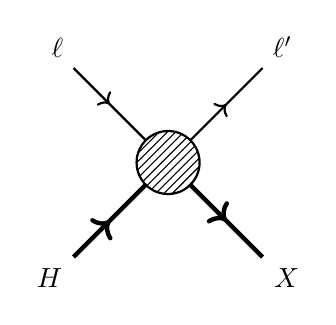
\begin{tikzpicture}[scale=0.8]
\begin{scope}[thick,decoration={
    markings,
    mark=at position 0.5 with {\arrow{>}}}
    ] 
\draw[postaction = {decorate}, ultra thick] (-1.5,-1.5) node[below left]{$H$} -- (-0.35,-0.35);
\draw[postaction = {decorate}] (-1.5,1.5) node[above left]{$\ell$} -- (-0.35,0.35) ;
\draw[postaction = {decorate}, ultra thick] (0.35,-0.35) -- (1.5,-1.5) node[below right]{$X$};
\draw[postaction = {decorate}] (0.35,0.35) -- (1.5,1.5) node[above right]{$\ell'$};
\end{scope}

\fill[pattern=north east lines] circle(0.5cm) (0,0);
\draw[thick] circle(0.5cm) (0,0);
%\draw[thick, snake it] (0,0) -- (1.5,0) node[right]{$B$};
\end{tikzpicture}
\caption{Deep inelastic scattering (DIS) of a lepton $\ell$ on a hadron $H$, producing a lepton $\ell'$ and a hadronic state $X$.}
\label{fig:dis}
\end{figure}

\noindent The differential cross-section for this process, in $d$ spacetime dimensions, may be expressed as:
\begin{align}
\label{eq:diff_xsec_dis}
d\sigma &= \frac{1}{4 \sqrt{(p_{\ell} \cdot p_H)^2 - M_{\ell}^2 M_H^2}} \frac{d^{d-1}\vec{p}_{\ell'}}{(2\pi)^{d-1} 2E_{\ell'}} \sum_{X} \left(\prod_{i=1}^{n_X} \frac{d^{d-1} \vec{p}_{(i,X)}}{(2\pi)^{d-1} 2E_{(i,X)}}\right) \notag \\[1.5ex]
& \qquad\qquad \cdot (2\pi)^d \delta^d\left(p_\ell + p_H - p_{\ell'} - \sum_{i=1}^{n_X} p_{(i,X)}\right) \overline{\left| \mathcal{M}(\ell H \rightarrow \ell' X) \right|^2},
\end{align}
where the pair $(i,X)$ denotes the $i$th particle in the hadronic state $X$ (with $i$ in the range $i \in \{1,...,n_X\}$, for a total of $n_X$ particles in the state $X$), the four-vector $p_{P} = (E_{P}, \vec{p}_{P})$ is the four-momentum of the particle $P$, and $\mathcal{M}(\ell H \rightarrow \ell' X)$ is the amplitude for the process. The sum over $X$ indicates a sum over all possible hadronic states which can be produced in the collision, reflecting our desire to be blind towards the hadronic products. The bar over the modulus-squared amplitude denotes the spin/colour-sum/average; more precisely, we average over the possible spin/colour states of the initial states, and sum over the spin/colour states of the final states (note that for hadronic states $H,X$ the colour sum/average is trivial because hadronic states are colourless). The notation $M_{P}$ means the rest mass of the state $P$.

\begin{figure}[H]
\centering
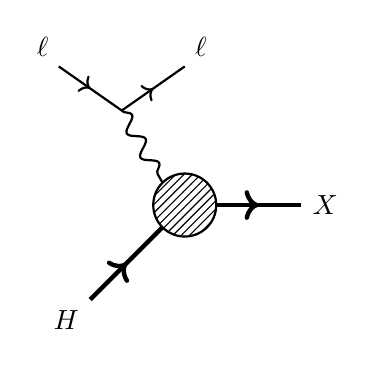
\begin{tikzpicture}[scale=0.8]
\begin{scope}[thick,decoration={
    markings,
    mark=at position 0.5 with {\arrow{>}}}
    ] 
\draw[postaction = {decorate}, ultra thick] (-1.5,-1.5) node[below left]{$H$} -- (-0.35,-0.35);
\draw[postaction = {decorate}, ultra thick] (0.5,0) -- (1.85,0) node[right]{$X$};

\draw[postaction = {decorate}] (-2,2.2) node[above left]{$\ell$} -- (-1,1.5) ;
\draw[postaction = {decorate}] (-1,1.5) -- (0,2.2) node[above right]{$\ell$};
\end{scope}

\fill[pattern=north east lines] circle(0.5cm) (0,0);
\draw[thick] circle(0.5cm) (0,0);
\draw[thick, snake it] (-1,1.5) -- (-0.35,0.35);
\end{tikzpicture}
\caption{Feynman diagram for DIS of an electron off a proton, mediated by a photon, to leading order in QED.}
\label{fig:photondis}
\end{figure}

For ease of exposition, let us now focus on the specific case where $\ell, \ell'$ are electrons, $H$ is a proton, and the process is mediated by a photon. The Feynman diagram for this process (working to leading order in QED for the photon-electron interactions) takes the form shown in Fig.~\ref{fig:photondis}. Thus, the amplitude may be expressed in the form:
\begin{equation}
\mathcal{M}(\ell H \rightarrow \ell'X) = (ie)^2 \bar{u}(p_{\ell'}) \gamma^{\mu} u(p_{\ell}) \cdot \frac{i}{q^2} \cdot \braket{X | J_{\mu} | H},
\end{equation}
where the factors of $ie$ arises from the electron-photon and electron-hadron interactions, the spinor algebra $\bar{u}(p_{\ell'}) \gamma^{\mu} u(p_{\ell})$ arises from the electron lines, the factor of $i/q^2$ comes from the photon propagator (where we have defined $q = p_{\ell} - p_{\ell'}$ to be the momentum of the virtual photon), and the matrix element $\braket{X | J_{\mu} | H}$ comes from the hadron-photon interaction in the lower half of the diagram. Here, $J_{\mu}$ is the electromagnetic current governing photon-quark interactions, given by:
\begin{equation}
J_{\mu} = \sum_{q} e_q \bar{q} \gamma_{\mu} q,
\end{equation}
where $e_q$ is the charge on a quark of flavour $q$, in units of the electron charge. Taking the spin/colour-sum/average of the modulus-squared amplitude, we obtain:
\begin{equation}
\overline{|\mathcal{M}(\ell H \rightarrow \ell'X)|^2} = \frac{e^4}{2q^4} \textrm{Tr}\left( \gamma^{\mu} \slashed{p}_{\ell} \gamma^{\nu} \slashed{p}_{\ell'} \right) \overline{\braket{H | J_{\nu}^{\dagger} | X}\braket{X | J_{\mu} | H}},
\end{equation}
where the bar over the amplitude denotes the spin/colour-sum/average. At this point, it is convenient to introduce two tensors in terms of which the differential cross-section can be parametrised. We define the \textit{leptonic tensor} via:
\begin{equation}
\label{eq:leptonic_tensor}
L^{\mu\nu} = e^4 \textrm{Tr}\left(  \gamma^{\mu} \slashed{p}_{\ell} \gamma^{\nu} \slashed{p}_{\ell'} \right) = 4e^4 \left( p_{\ell}^{\mu} p_{\ell'}^{\nu} + p_{\ell}^{\nu} p_{\ell'}^{\mu} - \eta^{\mu\nu} p_{\ell} \cdot p_{\ell'} \right),
\end{equation}
where the second form is obtained through basic gamma matrix identities, and the \textit{hadronic tensor} via:
\begin{align}
\label{eq:hadronic_tensor}
H_{\mu\nu} &= \frac{1}{4\pi} \sum_{X} \left(\prod_{i=1}^{n_X} \frac{d^{d-1} \vec{p}_{(i,X)}}{(2\pi)^{d-1} 2E_{(i,X)}}\right) \cdot (2\pi)^d \delta^d\left(p_\ell + p_H - p_{\ell'} - \sum_{i=1}^{n_X} p_{(i,X)}\right)  \overline{\braket{H | J_{\nu}^{\dagger} | X}\braket{X | J_{\mu} | H}}.
\end{align}
The differential cross-section may then be expressed in the simplified form:
\begin{equation}
\label{eq:almost_final_dis}
d\sigma = \frac{1}{4\sqrt{(p_{\ell} \cdot p_H)^2 - M_{\ell}^2 M_H^2}} \cdot \frac{1}{q^4} \frac{d^{d-1}\vec{p}_{\ell'}}{(2\pi)^{d-2} 2E_{\ell'}} L^{\mu\nu} H_{\mu\nu}.
\end{equation}
This form is particularly useful, since it clearly decomposes the differential cross section's dependence into a \textit{perturbative} part, namely the leptonic tensor, and a \textit{non-perturbative} part, namely the hadronic tensor. Hence, we have isolated the key challenge in computing a DIS cross-section: modelling the hadronic tensor.

Before commenting further on the hadronic tensor though, it is useful to perform some further superficial work to make Eq.~\eqref{eq:almost_final_dis} match with standard expressions in the literature (see for example Chapter 19 of Ref.~\cite{ParticleDataGroup:2022pth}). We begin by introducing the standard Lorentz-invariant kinematical variables $Q^2$, $x$ and $y$, defined by:
\begin{equation}
\label{eq:dis_kinematics}
Q^2 = -q^2, \qquad x = -\frac{q^2}{2q \cdot p_H}, \qquad y = \frac{q \cdot p_H}{p_{\ell} \cdot p_H}.
\end{equation}
The first invariant quantity is simply the \textit{virtuality} of the mediating photon; it has units of squared energy. The second invariant quantity is called the \textit{Bjorken-$x$}, and its interpretation will become clear when we discuss the parton model shortly. The third invariant quantity is called the \textit{inelasticity}, and measures the fraction of energy lost by the electron; we can see this by working in the rest frame of the hadron, $\vec{p}_H = \vec{0}$, which yields:
\begin{equation}
y = \frac{E_{\ell} - E_{\ell'}}{E_{\ell}} = 1 - \frac{E_{\ell'}}{E_{\ell}},
\end{equation}
where $E_{\ell}$ is the energy of the initial electron, and $E_{\ell'}$ is the energy of the final electron.

Working in four dimensions, $d=4$, we can change variables from $\vec{p}_{\ell'}$ in Eq.~\eqref{eq:almost_final_dis} via:
\begin{align}
d^{3} \vec{p}_{\ell'} &= |\vec{p}_{\ell'}|^{2} d|\vec{p}_{\ell'}| d\cos(\theta) d\phi = |\vec{p}_{\ell'}|^{2}\left|\det\left(\frac{\partial (|\vec{p}_{\ell'}|, \cos(\theta))}{\partial(x, y)}\right) \right| dx dy d\phi,
\label{eq:change_of_variables}
\end{align}
where $\theta$ is the angle defined by $\cos(\theta) := \vec{p}_{\ell} \cdot \vec{p}_{\ell'} / |\vec{p}_{\ell}| |\vec{p}_{\ell'}|$, and $d\phi$ is the remaining angular integral. To calculate the Jacobian matrix in Eq.~\eqref{eq:change_of_variables}, consider working in the rest frame of the proton, so that $\vec{p}_H = \vec{0}$. Then, assuming the masslessness of the electrons so that $E_{\ell} = |\vec{p}_{\ell}|$, $E_{\ell'} = |\vec{p}_{\ell'}|$, we can rewrite the variables in Eq.~\eqref{eq:dis_kinematics} through:
\begin{equation}
\label{eq:change_of_variables}
x = \frac{|\vec{p}_{\ell}| |\vec{p}_{\ell'}| \left(1 - \cos(\theta)\right)}{M_H (|\vec{p}_{\ell}| - |\vec{p}_{\ell'}|)}, \qquad y = 1 - \frac{|\vec{p}_{\ell'}|}{|\vec{p}_{\ell}|},
\end{equation}
where $M_H$ is the rest mass of the proton. Solving these equations simultaneously for $|\vec{p}_{\ell'}|$ and $\cos(\theta)$, we have:
\begin{equation}
|\vec{p}_{\ell'}| = |\vec{p}_{\ell}|(1-y), \qquad \cos(\theta) = 1 - \frac{M_H xy}{|\vec{p}_{\ell}|(1-y)}.
\end{equation}
This allows us to compute the Jacobian factor:
\begin{equation}
\left|\det\left(\frac{\partial (|\vec{p}_{\ell'}|, \cos(\theta))}{\partial(x, y)}\right) \right| = \frac{M_H y}{1-y}.
\end{equation}
Hence the measure in Eq.~\eqref{eq:change_of_variables} may be rewritten as:
\begin{equation}
d^{3} \vec{p}_{\ell'} =  |\vec{p}_{\ell}|^2 (1-y) M_H y \ dx dy d\phi.
\end{equation}
Putting everything together, the differential cross-section Eq.~\eqref{eq:almost_final_dis} may be written in the simple form:
\begin{equation}
\frac{d^3\sigma}{dx dy d\phi} = \frac{y}{32 \pi^2 Q^4} L^{\mu\nu} H_{\mu\nu}.
\end{equation}
To make further progress, we study the Lorentz structure of the hadronic tensor. As can be observed from the definition in Eq.~\eqref{eq:hadronic_tensor}, the only momenta on which the hadronic tensor can depend are the momentum of the initial hadron, $p_H$, and the difference in momentum between the outgoing and ingoing electron, $q$; that is, $H_{\mu\nu} \equiv H_{\mu\nu}(p_H, q)$. The only Lorentz scalars which can be constructed from $p_H$ and $q$ are $p_H^2 = M_H^2$, which is a fixed constant, $q^2 = -Q^2$ and $p_H \cdot q = Q^2/2x$. It can then be shown (see e.g. Ref.~\cite{Halzen:1984mc}) that current conservation at the hadronic vertex implies that the most general Lorentz-covariant structure for the hadronic tensor is given by:
\begin{equation}
H_{\mu\nu}(p_H, q) \equiv \left( -\eta_{\mu\nu} + \frac{q_{\mu} q_{\nu}}{q^2} \right) F_1(x,Q^2) + \left( p_{H\mu} - \frac{p_H \cdot q}{q^2} q_{\mu} \right) \left( p_{H\nu} - \frac{p_H \cdot q}{q^2} q_{\nu} \right) \frac{F_2(x,Q^2)}{p_H \cdot q},
\end{equation}
for some scalar functions $F_1, F_2$, called the \textit{neutral current DIS structure functions}.

Contracting with the expression for the leptonic tensor, Eq.~\eqref{eq:leptonic_tensor},\footnote{When performing this contraction, it is convenient to note that $q_{\mu} L^{\mu\nu} = 0$, by four-momentum conservation.} we arrive at the following expression for the differential cross-section:
\begin{equation}
\frac{d^3\sigma}{dx dy d\phi} = \frac{2y \alpha^2}{Q^4} \left( 2(p_{\ell} \cdot p_{\ell'}) F_1 + \frac{1}{p_H \cdot q} [2 (p_H \cdot p_{\ell}) (p_H \cdot p_{\ell'}) - M_H^2 (p_{\ell} \cdot p_{\ell'})] F_2 \right),
\end{equation}
where $\alpha = e^2 / 4\pi$ is the fine structure constant of QED. To finish, we note that Eq.~\eqref{eq:dis_kinematics} allow us to write:
\begin{equation}
p_{\ell} \cdot p_{\ell'} = \frac{Q^2}{2}, \qquad p_H \cdot p_{\ell} = \frac{Q^2}{2xy}, \qquad p_H \cdot p_{\ell'} = \frac{Q^2}{2x} \left( \frac{1}{y} - 1 \right). 
\end{equation}
Overall then, we can re-express the differential cross-section as:
\begin{equation}
\frac{d^3\sigma}{dx dy d\phi} = \frac{2\alpha^2}{xy Q^2} \left(xy^2F_1 + \left[1 - y - M_H^2 \frac{x^2y^2}{Q^2}\right] F_2\right).
\end{equation}
We see that the right hand side possesses no dependence on the angular variable $\phi$, so may be integrated directly to yield:
\begin{framed}
\begin{equation}
\frac{d^2\sigma}{dx dy} = \frac{4\pi\alpha^2}{xy Q^2} \left(xy^2F_1 + \left[1 - y - M_H^2 \frac{x^2y^2}{Q^2}\right] F_2 \right).
\end{equation}
\end{framed}
This is the final form for the (photon-mediated) DIS differential cross-section, in agreement with Eq. (19.8) of Ref.~\cite{ParticleDataGroup:2022pth}. It is written in terms of the structure functions, $F_1, F_2$, which are the experimentally accessible observables; modelling the hadronic tensor therefore provides predictions for the observable quantities in DIS.


\subsection{The parton model}
So far, the hadronic tensor remains incalculable in perturbation theory, since it depends on the non-perturbative proton state $\ket{H}$. In order to model it, Feynman proposed a phenomenological model called the \textit{parton model}, which we describe as follows. 

It was originally argued in \cite{Feynman:1969wa} that at ultra-relativistic energies (namely in the \textit{deep inelastic limit} $Q^2 \rightarrow \infty$, where the energy transferred from the electron to the proton through the virtual photon approaches infinity), relativistic time-dilation results in the interactions in the proton happening over a characteristic scale $O(1/Q)$. In particular, this implies that at the moment of collision, the impacting electron will interact with only a \textit{single} constituent of the proton. This suggests adopting the following phenomenological model, called the \textit{parton model}, for the hadronic tensor:
\begin{align}
\label{eq:parton_model_hadronic_tensor}
H_{\mu\nu} &= \frac{1}{4\pi} \sum_{q} \int\limits_{0}^{1} \frac{d\xi}{\xi} \sum_{X} \left(\prod_{i=1}^{n_X} \frac{d^{d-1} \vec{p}_{(i,X)}}{(2\pi)^{d-1} 2E_{(i,X)}}\right) \cdot (2\pi)^d \delta^d\left(p_\ell + \xi p_H - p_{\ell'} - \sum_{i=1}^{n_X} p_{(i,X)}\right)\notag \\[1.5ex]
&\qquad\qquad\qquad\qquad \cdot \overline{\braket{q(\xi p_H) | J_{\nu}^{\dagger} | X}\braket{X | J_{\mu} | q(\xi p_H) }} f_q(\xi),
\end{align}
Here, we have replaced the hadronic state $\ket{H}$ with a state $\ket{q(\xi p_H)}$; this denotes a state comprising a free constituent $q$ of the proton,\footnote{Note we also denote the virtuality of the mediating photon by $q$; this should cause no confusion as they enter in different ways.} carrying a fraction $\xi$ of the momentum of the proton $H$. We sum over all possible constituents $q$, and we weight the contributions by some unknown, non-perturbative probability distributions $f_q(\xi)$; these distributions represent the probability of the proton ejecting a constituent $q$ to interact with the electron, carrying a momentum fraction $\xi$. Naturally, we also integrate over all possible momentum fractions. The bar over the amplitude product denotes the spin/colour-sum/average, as usual.

With this assumption on the form of the hadronic tensor, we may calculate the hadronic tensor at lowest order in QCD perturbation theory. In this case, we may take $\ket{X}$ to be a single quark state $\ket{X} = \ket{q(p_X)}$;\footnote{Recall that $X$ was initially defined to be a hadronic state; however, since we are summing over all hadronic states by completeness we may choose to use a basis of quarks and gluons rather than a basis of hadrons, similar to the discussion given around Eqs.~\eqref{eq:completeness} and \eqref{eq:e+e-_completeness}.} then, the hadronic tensor reduces to:
\begin{align}
H_{\mu\nu}^{\text{LO}} &= \frac{1}{2} \sum_{q} \int\limits_{0}^{1} \frac{d\xi}{\xi} \int\frac{d^{d-1} \vec{p}_X}{ 2E_{X}} \delta^d\left(p_\ell + \xi p_H - p_{\ell'} - p_X\right)  \overline{\braket{q(\xi p_H) | J_{\nu}^{\dagger} | q(p_X)}\braket{q(p_X) | J_{\mu} | q(\xi p_H) }} f_q(\xi).
\end{align}
Note that in this case, the colour sum/average of the amplitude product is trivial, since the quark does not change colour during the interaction. The phase space integral can be manipulated via:
\begin{equation}
\int\frac{d^{d-1} \vec{p}_X}{ 2E_{X}} \delta^d\left(p_\ell + \xi p_H - p_{\ell'} - p_X\right) = \int d^d p_X \delta(p_X^2) \delta^d\left( p_{\ell} + \xi p_H - p_{\ell'} - p_X \right),
\end{equation}
which results in:
\begin{align}
H_{\mu\nu}^{\text{LO}} &= \frac{1}{2} \sum_{q}\int\limits_{0}^{1} \frac{d\xi}{\xi}\ \delta((q + \xi p_H)^2) \cdot \ \overline{\braket{q(\xi p_H) | J_{\nu}^{\dagger} | q(q + \xi p_H)}\braket{q(q + \xi p_H) | J_{\mu} | q(\xi p_H) }} f_q(\xi).
\end{align}
In the deep inelastic limit $Q^2 \rightarrow \infty$, corresponding to very high energy transfer from the electron to the proton, we have that $(q + \xi p_H)^2 = q^2 + 2 \xi q \cdot p_H + p_H^2 \approx q^2 + 2 \xi q \cdot p_H$, and hence the delta function condition can be rewritten as:
\begin{equation}
\delta(q^2 + 2 \xi q \cdot p_H) = \frac{\delta(x - \xi)}{2 q \cdot p_H},
\end{equation}
where $x$ is the Bjorken-$x$ we introduced earlier in the text; this reveals that, at leading order in QCD perturbation theory, the interpretation of the Bjorken-$x$ is the momentum fraction carried by the quark state ejected by the hadron which participates in the interaction with the photon. It follows that the hadronic tensor may be expressed in the parton model as:
\begin{align}
H_{\mu\nu}^{\text{LO}} &= \frac{1}{4 x q \cdot p_H} \sum_{q} \overline{\braket{q(x p_H) | J_{\nu}^{\dagger} | q(q + x p_H)}\braket{q(q + x p_H) | J_{\mu} | q(x p_H) }} f_q(x).
\end{align}
We can now straightforwardly compute the matrix elements to yield:
\begin{align}
&\overline{\braket{q(x p_H) | J_{\nu}^{\dagger} | q(q + x p_H)}\braket{q(q + x p_H) | J_{\mu} | q(x p_H) }} \notag\\
&\qquad= \frac{1}{2} e_q^2 \textrm{Tr}(x \slashed{p}_H \gamma_{\nu} (\slashed{q} + x \slashed{p}_H) \gamma_{\mu}) \\[1.5ex]
&\qquad = 2x e_q^2 \left( p_{H\nu} (q + x p_H)_{\mu} + p_{H\mu} (q + x p_H)_{\nu} - \eta_{\mu\nu} p_H \cdot (q + x p_H) \right),\notag
\end{align}
where $e_q$ is the charge on the quark $q$ in units of the electric charge $e$. Note the factor of $1/2$ coming from averaging the ejected quark spin states.

In the ultra-relativistic limit, it becomes appropriate to neglect the mass of the target proton, $M_H^2 \approx 0$; in this case, we can project the structure functions out of the hadronic tensor via the following contractions:
\begin{align}
\label{eq:hadronic_to_structure1}
F_1(x,Q^2) &=\left( -\frac{1}{2} \eta^{\mu\nu} + \frac{2x^2}{Q^2} p_H^{\mu} p_H^{\nu} \right) H_{\mu\nu} (p_H, q), \\[1.5ex]
\label{eq:hadronic_to_structure2}
F_2(x,Q^2) &= \left( - x \eta^{\mu\nu} + \frac{12x^3}{Q^2} p_H^{\mu} p_H^{\nu} \right) H_{\mu\nu}(p_H, q).
\end{align}
Applying the projectors, Eq.~\eqref{eq:hadronic_to_structure1} and Eq.~\eqref{eq:hadronic_to_structure2}, we obtain the following formulae for the structure functions (to leading order in QCD):
\begin{framed}
\begin{align}
F_1^{\text{LO}}(x,Q^2) &= \frac{1}{2}\sum_{q} e_q^2 f_q(x), \\[1.5ex]
F_2^{\text{LO}}(x,Q^2) &= x \sum_{q} e_q^2 f_q(x).
\end{align}
\end{framed}
Note the following important features of our final structure function formulae in the parton model:
\begin{enumerate}[label = (\arabic*)]
\item We have the relation $F_2^{\text{LO}} = 2x F_1^{\text{LO}}$. This identity is called the \textit{Callan-Gross relation}, and provides evidence that the primary constituents of the proton have spin-$\frac{1}{2}$; if we assume different spins for the constituents of the proton, and attempt to perform the calculations presented in this section, we obtain different relations between $F_1^{\text{LO}}, F_2^{\text{LO}}$ which are not observed experimentally (indeed one obtains $F_1^{\text{LO}}\equiv 0$ for scalar quarks, for example - see the discussion below Eq.~(4.18) in \cite{Ellis:1996mzs}). The Callan-Gross relation is not \textit{perfect}; deviations from this law are due to QCD corrections to the parton model, which we shall now discuss.
\item The structure functions are independent of $Q^2$; this is called \textit{Bjorken scaling}, and is experimentally observed when $Q^2 \rightarrow \infty$ (see for example Fig. 6 of Ref.~\cite{Martin:1994kn}). Similarly, Bjorken scaling is broken by QCD corrections to the parton model.
\end{enumerate}

\subsection{The QCD-improved parton model}
We can extend the parton model by including next-to-leading order QCD corrections. The diagrams which contribute to the next-to-leading order QCD corrections can be classified into two categories:
\begin{enumerate}[label = (\roman*)]
\item \textbf{Real and virtual gluon emission.} In this case, a gluon is emitted from either the initial quark leg, or the final quark leg (shown on the left and right of Fig.~\ref{fig:real_gluon_emission} respectively). We take the final state to be $\ket{X} = \ket{q(p_q) g(p_g)}$, comprising a quark of four-momentum $p_q$ and a gluon of four-momentum $p_g$.

Alternatively, a virtual gluon can be emitted from the initial or final quark leg and \textit{reabsorbed}, rather than radiated. We will not give the details of the calculation of these diagrams for brevity, merely stating the results (we shall see that an important cancellation occurs between the real and virtual diagram contributions).

\item \textbf{Gluon-boson fusion.} In this case, a gluon is ejected from the proton, splitting into two quarks; one of the quarks is radiated, whilst the other participates in an interaction with the photon (see Fig.~\ref{fig:gluon_boson_fusion}). Again, in the interest of being brief, we will not give the details of this calculation, simply stating the complete results at the end of the discussion.
\end{enumerate}

\begin{figure}
\centering
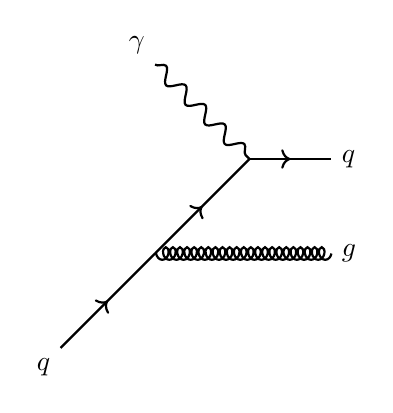
\begin{tikzpicture}[scale=0.8]
\begin{scope}[thick,decoration={
    markings,
    mark=at position 0.5 with {\arrow{>}}}
    ] 
\draw[postaction = {decorate}, thick] (-1.5,-1.5) node[below left]{$q$} -- (0,0);
\draw[postaction = {decorate}, thick] (0,0) -- (1.5,1.5);
\draw[postaction = {decorate}, thick] (1.5,1.5) -- (2.8,1.5) node[right]{$q$};
\end{scope}

%\fill[pattern=north east lines] circle(0.5cm) (0,0);
%\draw[thick] circle(0.5cm) (0,0);
\draw[thick, snake it] (0,3) node[above left]{$\gamma$} -- (1.5,1.5);
\draw[decoration={aspect=0.7, segment length=0.9mm, amplitude=0.8mm,coil}, decorate, thick] (2.8,0) node[right]{$g$} -- (0,0);
\end{tikzpicture}
\hspace{3cm}
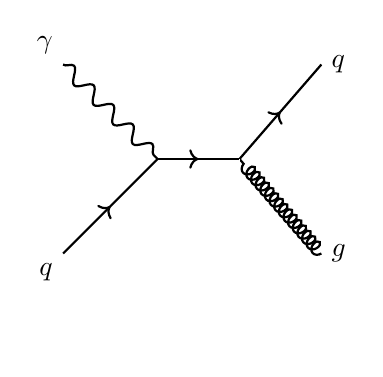
\begin{tikzpicture}[scale=0.8]
\begin{scope}[thick,decoration={
    markings,
    mark=at position 0.5 with {\arrow{>}}}
    ] 
%\draw[postaction = {decorate}, thick] (-1.5,-1.5) node[below left]{$q$} -- (0,0);
\draw[postaction = {decorate}, thick] (0,0) node[below left]{$q$} -- (1.5,1.5);
\draw[postaction = {decorate}, thick] (1.5,1.5) -- (2.8,1.5);
\draw[postaction = {decorate}, thick] (2.8,1.5) -- (4.1,3) node[right]{$q$};
\end{scope}

%\fill[pattern=north east lines] circle(0.5cm) (0,0);
%\draw[thick] circle(0.5cm) (0,0);
\draw[thick, snake it] (0,3) node[above left]{$\gamma$} -- (1.5,1.5);
\draw[decoration={aspect=0.7, segment length=0.9mm, amplitude=0.8mm,coil}, decorate, thick] (4.1,0) node[right]{$g$} -- (2.8,1.5);
\draw[color=white] (2.8,1.5) -- (2.8,-1.5);
\end{tikzpicture}
\caption{\textbf{Left.} Real gluon emission from the initial quark. \textbf{Right.} Real gluon emission from the final quark.}
\label{fig:real_gluon_emission}
\end{figure}

\begin{figure}
\centering
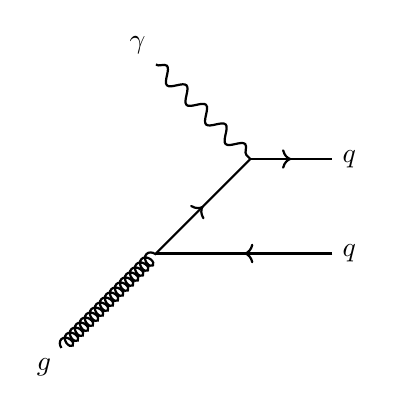
\begin{tikzpicture}[scale=0.8]
\begin{scope}[thick,decoration={
    markings,
    mark=at position 0.5 with {\arrow{>}}}
    ] 
\draw[postaction = {decorate}, thick] (2.8,0) node[right]{$q$} -- (0,0);
\draw[postaction = {decorate}, thick] (0,0) -- (1.5,1.5);
\draw[postaction = {decorate}, thick] (1.5,1.5) -- (2.8,1.5) node[right]{$q$};
\end{scope}

%\fill[pattern=north east lines] circle(0.5cm) (0,0);
%\draw[thick] circle(0.5cm) (0,0);
\draw[thick, snake it] (0,3) node[above left]{$\gamma$} -- (1.5,1.5);
\draw[decoration={aspect=0.7, segment length=0.9mm, amplitude=0.8mm,coil}, decorate, thick] (-1.5,-1.5) node[below left]{$g$} -- (0,0);
\end{tikzpicture}
\caption{Ejection of a gluon from the proton, splitting into a quark which participates in the hard reaction with the photon, and a quark which is radiated. There is also a similar diagram involving antiquarks, where the arrows on the fermion lines are reversed.}
\label{fig:gluon_boson_fusion}
\end{figure}

We begin by computing the contribution to the hadronic tensor from (i), specifically focussing on real gluon emission. Throughout we work in $d$ dimensions, so that we may employ dimensional regularisation when subsequently regulating the theory (we shall find that there are divergences in the calculation). The amplitudes for the diagrams in Fig.~\ref{fig:real_gluon_emission} are, respectively:
\begin{align}
\mathcal{M}_{\mu}^i &= -i g_S \mu^{\epsilon} e_q \bar{u}(p_{q}) \gamma_{\mu} \frac{1}{\xi \slashed{p}_H - \slashed{p}_{g}}\slashed{\epsilon}(p_{g}) t^A u(\xi p_H)  \\[1.5ex]
\mathcal{M}_{\mu}^f &= -i g_S \mu^{\epsilon} e_q \bar{u}(p_q) \slashed{\epsilon}(p_g) \frac{1}{\slashed{p}_q + \slashed{p}_g} \gamma_{\mu} t^A u(\xi p_H),
\end{align}
where $g_S\mu^{\epsilon}$ is the coupling constant of QCD in $d$ dimensions; this is the $d$-dimensional version of the coupling $g_S$ appearing in Eq.~\eqref{eq:qcd_derivative}, but now includes an additional factor of $\mu^{\epsilon}$ where $\mu$ is an arbitrary mass scale and $\epsilon = \frac{4 - d}{2}$. The polarisation of the gluon is given by $\epsilon_{\mu}(p_g)$. The factor of $t^A$ denotes the relevant colour matrix from the Lie algebra $\mathfrak{su}_{\mathbb{C}}(3)$; technically this implies that $\mathcal{M}_{\mu}^i$ should also carry an $SU(3)$-index $A$ corresponding to the colour state of the emitted gluon, but we will suppress this given that we will shortly sum/average over colours. The labels $i,f$ on the respective amplitudes denote a gluon emitted from the \textit{i}nitial quark and the \textit{f}inal quark.

In this case, the contribution to the hadronic tensor is given by:
\begin{align}
\label{eq:hadronic_nlo_real}
H_{\mu\nu}^{\text{NLO, real}} &= \frac{1}{4\pi} \sum_{q} \int\limits_{0}^{1} \frac{d\xi}{\xi} f_q(\xi) \int \frac{d^{d-1} \vec{p}_{q}}{(2\pi)^{d-1} 2E_{q}}  \frac{d^{d-1} \vec{p}_{g}}{(2\pi)^{d-1} 2E_{g}} \notag\\[1.5ex]
&\qquad\qquad\cdot (2\pi)^d \delta^d\left(q + \xi p_H - p_q - p_g\right) \cdot \sum_{r,s=i,f} \overline{\mathcal{M}_{\mu}^r \mathcal{M}_{\nu}^{s\dagger}} ,
\end{align}
where, as usual, the bar on the amplitude product denotes the spin/colour-sum/average. This expression can be evaluated in two steps: first, we will manipulate the phase space into a more amenable form, and then second, we shall compute the spin/colour-sum/averages of the amplitude products.

We begin by noting that:
\begin{align}
&\int \frac{d^{d-1} \vec{p}_{q}}{(2\pi)^{d-1} 2E_{q}}  \frac{d^{d-1} \vec{p}_{g}}{(2\pi)^{d-1} 2E_{g}} \cdot (2\pi)^d \delta^d\left(q + \xi p_H - p_q - p_g\right) \notag\\[1.5ex]
&\qquad= \frac{1}{2(2\pi)^{d-2}} \int  \frac{d^{d-1} \vec{p}_{g}}{E_{g}} d^d p_q\ \delta(p_q^2) \delta^d\left(q + \xi p_H - p_q - p_g\right)\notag\\[1.5ex]
&\qquad= \frac{1}{2(2\pi)^{d-2}} \int \frac{d^{d-1} \vec{p}_{g}}{E_{g}} \delta( (q + \xi p_H - p_g)^2) 
\end{align}
To absorb the remaining delta function, we make a sequence of variable changes. Consider first changing variables from $\vec{p}_g$ to $(|\vec{p}_g|^2, \cos(\theta))$, where $\theta$ is the angle defined by:
\begin{equation}
\cos(\theta) = \frac{\vec{p}_g \cdot \xi \vec{p}_H}{|\vec{p}_g| |\xi \vec{p}_H|} = \frac{\vec{p}_g \cdot \vec{p}_H}{|\vec{p}_g| |\vec{p}_H|}.
\end{equation}
The measure transforms as:\footnote{Recall the gluon is real, so on-shell, and hence $E_g = |\vec{p}_g|$.}
\begin{align}
\int \frac{d^{d-1} \vec{p}_g}{E_g} &= \frac{1}{2} \int |\vec{p}_g|^{d-4} \sin^{d-4}(\theta) d(|\vec{p}_g|^2) d(\cos(\theta)) d\Omega_{d-3}\notag \\[1.5ex]
&= \frac{(d-2) \pi^{\frac{1}{2}(d-2)}}{2\Gamma(d/2)} \int  |\vec{p}_g|^{d-4} \sin^{d-4}(\theta) d(|\vec{p}_g|^2) d(\cos(\theta)) \notag\\[1.5ex]
&= \frac{\pi^{1-\epsilon}}{\Gamma(1-\epsilon)} \int  |\vec{p}_g|^{d-4} \sin^{d-4}(\theta) d(|\vec{p}_g|^2) d(\cos(\theta)),
\end{align}
where $d\Omega_{d-3}$ contains all angular integrations in $d-3$ dimensions, except for the integration over $\theta$; in the second line we perform the integration over $d\Omega_{d-3}$ using a standard hyperspherical integral, and in the final line we recall that $d = 4 - 2\epsilon$.

We now make a second change of variables. Consider introducing the variables $u,v$ defined by the conditions:
\begin{equation}
\label{eq:soft_and_collinear_definitions}
p_g \cdot p_q = \frac{Q^2}{2} \left( \frac{1-u}{u} \right), \qquad p_g \cdot \xi p_H = \frac{Q^2 v}{2u}.
\end{equation}
The interpretation of these variables will become clear shortly. In order to relate the variables $u,v$ to the variables $|\vec{p}_g|^2$, $\cos(\theta)$, we work in the centre of momentum frame where $\vec{q} + \xi \vec{p}_H = \vec{0} = \vec{p}_g + \vec{p}_q$. The four-vectors $q, \xi p_H, p_g, p_q$ can then be expressed as:
\begin{equation}
q = \begin{pmatrix} \sqrt{\xi^2 |\vec{p}_H|^2 - Q^2} \\ -\xi \vec{p}_H \end{pmatrix}, \quad \xi p_H = \begin{pmatrix} \xi |\vec{p}_H| \\ \xi \vec{p}_H  \end{pmatrix}, \quad p_g = \begin{pmatrix} |\vec{p}_g| \\ \vec{p}_g \end{pmatrix}, \quad p_q = \begin{pmatrix} |\vec{p}_g| \\ -\vec{p}_g \end{pmatrix},
\end{equation}
where the first component of the virtual photon's four-momentum can be computed by enforcing the condition $q^2 = -Q^2$. Using the definition of $u$ from $p_g \cdot p_q$, and working in the above frame, we see that:
\begin{equation}
|\vec{p}_g|^2 = \frac{Q^2}{4} \left( \frac{1-u}{u} \right).
\end{equation}
In particular, we see that $u$ describes the \textit{energy} of the radiated gluon; in particular, the limit $u \rightarrow 1$ corresponds to the limit in which the energy of the gluon goes to zero, the so-called \textit{soft} limit. 

To obtain a relation between $v$ and $|\vec{p}_g|, \cos(\theta)$, we note that by conservation of energy, we can deduce that:
\begin{equation}
 \sqrt{\xi^2 |\vec{p}_H|^2 - Q^2} + \xi |\vec{p}_H| = 2 |\vec{p}_g| \qquad \Rightarrow \qquad  \xi |\vec{p}_H| = \frac{4 |\vec{p}_g|^2 + Q^2}{4|\vec{p}_g|}.
\end{equation}
Then the definition of $v$ in terms of $p_g \cdot \xi p_H$, we have:
\begin{align}
\frac{Q^2 v}{2u} &= |\vec{p}_g| \xi | \vec{p}_H| - \vec{p}_g \cdot \xi \vec{p}_H \notag\\[1.5ex]
&= |\vec{p}_g| \xi |\vec{p}_H| (1 - \cos(\theta)) \notag\\[1.5ex]
&= \frac{Q^2}{4u}(1 - \cos(\theta)),
\end{align}
which yields:
\begin{equation}
v = \frac{1 - \cos(\theta)}{2}.
\end{equation}
Hence $v$ is a measure of the \textit{collinearity} of the outgoing quark and the radiated gluon; in particular, as $v \rightarrow 0$, we have the outgoing quark and the radiated gluon are collinear.

Computing the Jacobian factor, we can now make the change of variables to $u,v$. We note that:
\begin{equation}
d(|\vec{k}_g|^2) d\cos(\theta) = \frac{\partial(|\vec{k}_g|^2, \cos(\theta))}{\partial(u,v)} du dv = \frac{Q^2}{2u^2} du dv,
\end{equation}
and hence it follows that the phase space can be written in terms of $u, v$ as:
\begin{equation}
\frac{1}{2(2\pi)^{2 - 2\epsilon}} \frac{\pi^{1-\epsilon}}{2\Gamma(1-\epsilon)} Q^{2(1-\epsilon)} \int  du dv\ \frac{(1-u)^{-\epsilon}}{u^{2-\epsilon}} v^{-\epsilon} (1-v)^{-\epsilon} \delta( (q + \xi p_H - p_g)^2).
\end{equation}
To finish, we note that the argument of the delta function can be expanded to:
\begin{equation}
(q + \xi p_H - p_g)^2 = q^2 + 2 q \cdot \xi p_H - 2 q \cdot p_g - 2 \xi p_H \cdot p_g.
\end{equation}
Using Eq.~\eqref{eq:soft_and_collinear_definitions}, we can obtain the missing inner products of four-vectors which we require in evaluating this expression. We find that:
\begin{equation}
(q + \xi p_H - p_g)^2 = \delta\left( Q^2 \left( \frac{1}{u} - \frac{\xi}{x} \right) \right) = \frac{x\delta(\xi - x/u)}{Q^2},
\end{equation}
Using the delta function to absorb the $\xi$ integral in the hadronic tensor, we see that we have reduced the hadronic tensor to:

\begin{align}
\label{eq:hadronic_nlo_real_phase_space}
H_{\mu\nu}^{\text{NLO, real}} &= \frac{1}{4\pi} \sum_{q}\frac{1}{2(2\pi)^{2 - 2\epsilon}} \frac{\pi^{1-\epsilon}}{2\Gamma(1-\epsilon)} Q^{-2\epsilon} \int  du dv\ f_q\left( \frac{x}{u} \right) \frac{(1-u)^{-\epsilon}}{u^{1-\epsilon}} v^{-\epsilon} (1-v)^{-\epsilon} \sum_{r,s=i,f} \overline{\mathcal{M}_{\mu}^r \mathcal{M}_{\nu}^{s\dagger}} \\[1.5ex]
&= \frac{1}{32 \pi ^2 \Gamma(1 - \epsilon)} \left( \frac{4\pi}{Q^2} \right)^{\epsilon} \sum_{q} \int\limits_{x}^{1} \frac{du}{u} f_q\left( \frac{x}{u} \right) \frac{u^{\epsilon}}{(1-u)^{\epsilon}} \int\limits_{0}^{1} dv\ v^{-\epsilon} (1-v)^{-\epsilon} \sum_{r,s=i,f} \overline{\mathcal{M}_{\mu}^r \mathcal{M}_{\nu}^{s\dagger}}.
\label{eq:hadronic_nlo_real_phase_space_2}
\end{align}
The integration ranges can be obtained by considering the allowed regions of $u,v$ arising from their definitions in Eq.~\eqref{eq:soft_and_collinear_definitions}.\\

\noindent It remains to compute the spin/colour-sum/averages of the quantities quadratic in the amplitudes, $\overline{\mathcal{M}_{\mu}^r \mathcal{M}_{\nu}^{s\dagger}}$. Here, we shall only compute $\overline{\mathcal{M}_{\mu}^i \mathcal{M}_{\nu}^{i\dagger}}$ to demonstrate the details of such a calculation; the others can be obtained by similar means. We begin by observing that:
\begin{equation}
\label{eq:nlo_amplitude_squared}
\overline{\mathcal{M}_{\mu}^i \mathcal{M}_{\nu}^{i\dagger}} = \frac{e_q^2 g_S^2 \mu^{2\epsilon} C_F}{2(\xi p_H - p_g)^4} g^{\alpha\beta}_{\perp}(k_g) \textrm{Tr}\left( \slashed{p}_q \gamma_{\mu} (\xi \slashed{p}_H - \slashed{p}_g) \gamma_{\alpha} \xi \slashed{p}_H \gamma_{\beta} (\xi \slashed{p}_H - \slashed{p}_g) \gamma_{\nu} \right).
\end{equation}
The trace arises from the usual method of taking spin-sum/averages of spinors. The factor of $C_F = 4/3$ arises from the colour-sum/averages; in particular, it is the quadratic Casimir of $\mathfrak{su}_{\mathbb{C}}(3)$, obeying:
\begin{equation}
\sum_{A} (t^A)^2 = C_F I.
\end{equation}
Finally, the factor of $g^{\alpha\beta}_{\perp}(k_g)$ arises from the spin-sum/average of the radiated gluon; it is given by:
\begin{equation}
g^{\alpha\beta}_{\perp}(k_g) := \sum_{\text{polarisations}} \epsilon^{\alpha}(k_g) \epsilon^{\beta*}(k_g).
\end{equation} 
The sum depends on which polarisations are allowed in the final state. To simplify things as much as possible, we shall assume that \textit{all} polarisations are allowed, including unphysical ones. This requires us to also consider the introduction of ghost fields; however, fortunately at this order in QCD there are no diagrams which include the ghosts. Therefore, we can happily conclude that:
\begin{equation}
g^{\alpha\beta}_{\perp}(k_g) = \sum_{\text{polarisations}} \epsilon^{\alpha}(k_g) \epsilon^{\beta*}(k_g) = \eta^{\alpha\beta},
\end{equation}
the standard result when all polarisations are considered. This allows us to reduce Eq.~\eqref{eq:nlo_amplitude_squared} to the simplified form:
\begin{align}
\overline{\mathcal{M}_{\mu}^i \mathcal{M}_{\nu}^{i\dagger}} &= \frac{e_q^2 g_S^2 \mu^{2\epsilon} C_F}{8(\xi p_H \cdot k_g)^2} \textrm{Tr}\left( \slashed{p}_q \gamma_{\mu} (\xi \slashed{p}_H - \slashed{p}_g) \gamma_{\alpha} \xi \slashed{p}_H \gamma^{\alpha} (\xi \slashed{p}_H - \slashed{p}_g) \gamma_{\nu} \right)\notag\\[1.5ex]
&= \frac{2 (1-\epsilon) e_q^2 g_S^2 \mu^{2\epsilon} C_F}{\xi p_H \cdot p_g}  \left( \eta_{\mu\nu} p_g \cdot p_q - (p_g)_{\mu} (p_q)_{\nu} - (p_g)_{\nu} (p_q)_{\mu}\right),
\end{align}
where the trace can be evaluated by standard Dirac algebra methods.\footnote{Note that in the case where a $Z$-boson or a $W$-boson mediates deep inelastic scattering, rather than a photon, these traces additionally contain $\gamma^5$ matrices. The definition of $\gamma^5$ in $d = 4 - 2\epsilon$ dimensions is rather subtle, and a lot more care is required in these calculations. A detailed discussion can be found in \cite{Collins:1984xc}.} The factor of $1-\epsilon$ arises from a contraction of the form $\eta^{\alpha\beta} \eta_{\alpha\beta} = d = 4 - 2\epsilon$, recalling that we are working in $d = 4-2\epsilon$ dimensions.

Evaluating the other spin/colour-sum/averages of the quantities quadratic in the amplitudes, it can be shown that we have the following projections:
\begin{align}
-\eta^{\mu\nu} \sum_{r,s=i,f} \overline{\mathcal{M}_{\mu}^r \mathcal{M}_{\nu}^{s\dagger}} &= 4 e_q^2 g_S^2 \mu^{2\epsilon} C_F (1-\epsilon) \left[ (1-\epsilon) \left( \frac{p_g \cdot p_q}{p_g \cdot \xi p_H} + \frac{p_g \cdot \xi p_H}{p_g \cdot p_q}\right) + \frac{Q^2 (\xi p_H \cdot p_q)}{(p_g \cdot \xi p_H) (p_g \cdot p_q)} + 2\epsilon\right],\\[1.5ex]
p_H^{\mu} p_H^{\nu} \sum_{r,s=i,f} \overline{\mathcal{M}_{\mu}^r \mathcal{M}_{\nu}^{s\dagger}} &= \frac{4 e_q^2 g_S^2 \mu^{2\epsilon} C_F (1-\epsilon)}{\xi^2} (p_q \cdot \xi p_H).
\end{align}
These projections can be rewritten conveniently in terms of the `softness' and `collinearity' variables $u,v$ we introduced in Eq.~\eqref{eq:soft_and_collinear_definitions}:
\begin{align}
-\eta^{\mu\nu} \sum_{r,s=i,f} \overline{\mathcal{M}_{\mu}^r \mathcal{M}_{\nu}^{s\dagger}} &= 4 e_q^2 g_S^2 \mu^{2\epsilon} C_F (1-\epsilon) \left[ (1-\epsilon) \left( \frac{1-u}{v} + \frac{v}{1-u}\right) + \frac{2u(1-v)}{v(1-u)} + 2\epsilon\right],\\[1.5ex]
p_H^{\mu} p_H^{\nu} \sum_{r,s=i,f} \overline{\mathcal{M}_{\mu}^r \mathcal{M}_{\nu}^{s\dagger}} &= \frac{2 e_q^2 g_S^2 \mu^{2\epsilon} C_F (1-\epsilon) Q^2 (1-v) u}{x^2}.
\end{align}
Inserting these formulae into the appropriate projections of Eq.~\eqref{eq:hadronic_nlo_real_phase_space_2}, we obtain:
\begin{align}
\label{eq:real_transverse_unsimplified}
-\eta^{\mu\nu} H_{\mu\nu}^{\text{NLO, real}} &= \frac{\alpha_S C_F  (1-\epsilon)}{2\pi \Gamma(1 - \epsilon)} \left( \frac{4\pi \mu^2}{Q^2} \right)^{\epsilon} \sum_{q} e_q^2 \int\limits_{x}^{1} \frac{du}{u} f_q\left( \frac{x}{u} \right) \frac{u^{\epsilon}}{(1-u)^{\epsilon}} \notag\\[1.5ex]
& \qquad\qquad \cdot \int\limits_{0}^{1} dv\ v^{-\epsilon} (1-v)^{-\epsilon}  \left[ (1-\epsilon) \left( \frac{1-u}{v} + \frac{v}{1-u}\right) + \frac{2u(1-v)}{v(1-u)} + 2\epsilon\right],\\[1.5ex]
p^{\mu}_H p^{\nu}_H H_{\mu\nu}^{\text{NLO, real}} &=\frac{\alpha_S Q^2 C_F (1-\epsilon)}{4\pi x^2 \Gamma(1 - \epsilon)} \left( \frac{4\pi \mu^2}{Q^2} \right)^{\epsilon} \sum_{q} e_q^2 \int\limits_{x}^{1} \frac{du}{u} f_q\left( \frac{x}{u} \right) \frac{u^{1 + \epsilon}}{(1-u)^{\epsilon}} \int\limits_{0}^{1} dv\ v^{-\epsilon} (1-v)^{1-\epsilon},
\end{align}
where $\alpha_S = g_S^2 / 4\pi$ is the strong coupling. We wish to determine the behaviour of these expressions as $\epsilon \rightarrow 0$, i.e. as we restore $d=4$ dimensions. We note that the projection $p^{\mu}_H p^{\nu}_HH_{\mu\nu}^{\text{NLO, real}}$ remains finite in this limit, giving the result:
\begin{equation}
p^{\mu}_H p^{\nu}_H H_{\mu\nu}^{\text{NLO, real}} =\frac{\alpha_S Q^2 C_F}{8\pi x^2} \sum_{q} e_q^2 \int\limits_{x}^{1} du f_q\left( \frac{x}{u} \right).
\end{equation}
On the other hand, the projection $-\eta^{\mu\nu} H_{\mu\nu}^{\text{NLO, real}}$ is singular as $\epsilon \rightarrow 0$, and requires a more careful treatment. To begin with, we note that we can evaluate the collinear $v$ integral using the identity:\footnote{Technically this result holds only when $\Re(p), \Re(q) > 0$, but we can always pretend that $\epsilon$ is an appropriate range before using analytic continuation to justify whichever final result we get.}
\begin{equation}
\int\limits_{0}^{1} dv\ v^{p-1} (1-v)^{q-1} = \frac{\Gamma(p)\Gamma(q)}{\Gamma(p+q)}.
\end{equation} 
Applying this result repeatedly, we can simplify Eq.~\eqref{eq:real_transverse_unsimplified} to:
\begin{align}
&-\eta^{\mu\nu} H_{\mu\nu}^{\text{NLO, real}} = \frac{\alpha_S C_F  (1-\epsilon)}{2\pi \Gamma(1 - \epsilon)} \left( \frac{4\pi \mu^2}{Q^2} \right)^{\epsilon} \sum_{q} e_q^2 \int\limits_{x}^{1} \frac{du}{u} f_q\left( \frac{x}{u} \right) \frac{u^{\epsilon}}{(1-u)^{\epsilon}} \notag\\[1.5ex]
& \ \cdot \left[ (1-\epsilon) \left(  \frac{(1-u)\Gamma(-\epsilon)\Gamma(1-\epsilon)}{\Gamma(1 - 2\epsilon)} +  \frac{\Gamma(2 - \epsilon) \Gamma(1-\epsilon)}{(1-u)\Gamma(3 - 2\epsilon)} \right) + \frac{2u}{1-u} \frac{\Gamma(-\epsilon)\Gamma(2-\epsilon)}{\Gamma(2 - 2\epsilon)} + 2\epsilon \frac{\Gamma(1-\epsilon)^2}{\Gamma(2-2\epsilon)} \right],
\end{align}
which by repeated application of the functional equation of the gamma function, $\Gamma(x+1) = x\Gamma(x)$, may be reduced to the more convenient form:
\begin{align}
-\eta^{\mu\nu} H_{\mu\nu}^{\text{NLO, real}} &= \frac{\alpha_S C_F  (1-\epsilon) \Gamma(1-\epsilon)}{2\pi \Gamma(1 - 2\epsilon)} \left( \frac{4\pi \mu^2}{Q^2} \right)^{\epsilon} \sum_{q} e_q^2 \int\limits_{x}^{1} \frac{du}{u} f_q\left( \frac{x}{u} \right) \frac{u^{\epsilon}}{(1-u)^{\epsilon+1}} \notag\\[1.5ex]
&\qquad \cdot \left[ \left( -\frac{1}{\epsilon} + 1\right)(1-u)^2 +  \frac{1-\epsilon}{2(1-2\epsilon)} - \frac{2u(1-\epsilon)}{\epsilon(1-2\epsilon)} + \frac{2\epsilon}{1 - 2\epsilon} \right].
\label{eq:collinear_singularity}
\end{align}
We must now Laurent expand this formula in small $\epsilon$. The key result we shall require is:
\begin{equation}
\label{eq:plus_identity}
\frac{u^{\epsilon}}{(1-u)^{\epsilon+1}} = -\frac{1}{\epsilon} \delta(1-u) + \left( \frac{1}{1-u} \right)_+ - \epsilon \left( \frac{\log(1-u)}{1-u} \right)_+ + \epsilon \frac{\log(u)}{1-u} + O(\epsilon^2),
\end{equation}
which holds only in a distributional sense.\footnote{That is, when integrated against a smooth function from $u=0$ to $u=1$.} A proof of this identity is given in App.~\ref{app:plus_prescription}. Here, the $+$ symbol denotes the \textit{plus distribution}, defined by:
\begin{equation}
\int\limits_{0}^{1} F(u)_+ G(u)\ du = \int\limits_{0}^{1} F(u)(G(u) - G(1))\ du.
\end{equation}
Combining the identity Eq.~\eqref{eq:plus_identity} with the standard Laurent expansions of the rational function expression in the large square brackets, as $\epsilon \rightarrow 0$ we see that the projection $-\eta^{\mu\nu} H_{\mu\nu}^{\text{NLO, real}}$ behaves as:
\begin{align}
&-\eta^{\mu\nu} H_{\mu\nu}^{\text{NLO, real}} = \frac{\alpha_S C_F  (1-\epsilon) \Gamma(1-\epsilon)}{2\pi \Gamma(1 - 2\epsilon)} \left( \frac{4\pi \mu^2}{Q^2} \right)^{\epsilon} \sum_{q} e_q^2 \int\limits_{x}^{1} \frac{du}{u} f_q\left( \frac{x}{u} \right) \bigg[ \left( \frac{2}{\epsilon^2} + \frac{3}{2\epsilon} + \frac{7}{2} \right) \delta(1-u) \notag\\[1.5ex]
&\qquad- \frac{1}{\epsilon} \frac{1 + u^2}{(1-u)_+} + 3 - u - \frac{3}{2(1-u)_+} + (1+u^2) \left( \frac{\log(1-u)}{1-u} \right)_+ - \frac{1+u^2}{1-u} \log(u) + O(\epsilon)\bigg].
\end{align}
We see that there is a double pole as $\epsilon \rightarrow 0$; the origin of this can be traced back to the soft singularity as $u\rightarrow 1$ (this is made manifest in Eq.~\eqref{eq:plus_identity}), combined with the collinear singularity as $v \rightarrow 0$ (this is made manifest in Eq.~\eqref{eq:collinear_singularity}, since after we have performed the $v$ integration, we obtain a $1/\epsilon$ term).\\

\noindent We must sum the real gluon emissions with the virtual gluon emissions, which enter at the same order in QCD, and multiply the same quark distributions $f_q(\xi)$ in the parton model for the hadronic tensor. The calculation of these diagrams is equally long and arduous,\footnote{Though it is possible to use some physical arguments to reduce the workload, see e.g. the discussion around Eq.~(4.70) of Ref.~\cite{Ellis:1996mzs}.} so we shall merely state the complete results here. We find that in the limit as $\epsilon \rightarrow 0$, we obtain the contribution:
\begin{align}
\label{eq:virtual_transverse_unsimplified}
-\eta^{\mu\nu} H_{\mu\nu}^{\text{NLO, virtual}} &= -\frac{\alpha_S C_F  (1-\epsilon) \Gamma(1-\epsilon)}{2\pi \Gamma(1 - 2\epsilon)} \left( \frac{4\pi \mu^2}{Q^2} \right)^{\epsilon} \sum_{q} e_q^2 \int\limits_{x}^{1} \frac{du}{u} f_q\left( \frac{x}{u} \right) \delta(1-u) \notag\\[1.5ex]
& \qquad\qquad\qquad\qquad\qquad \cdot \left( \frac{2}{\epsilon^2} + \frac{3}{\epsilon} + 8 + \frac{\pi^2}{3} + O(\epsilon)\right)
\end{align}
with $p^{\mu}_H p^{\nu}_H H_{\mu\nu}^{\text{NLO, virtual}}$ vanishing as $\epsilon \rightarrow 0$. We note that the double pole, the $O(\epsilon^{-2})$ term, is cancelled exactly between the real and virtual corrections.\\

%\noindent The calculation of the second class of diagrams, namely the gluon-initiated gluon-boson fusion diagrams (ii), proceeds similarly and, for brevity, we omit the details of the calculation in this thesis. We obtain the following projections in this case, in the limit as $\epsilon \rightarrow 0$:
%\begin{align}
%-\eta^{\mu\nu} H_{\mu\nu}^{\text{NLO, gluon}} &= \frac{\alpha_S T_R (1-\epsilon) \Gamma(1-\epsilon)}{\pi \Gamma(1-2\epsilon)} \left( \frac{4 \pi \mu^2}{Q^2} \right)^{\epsilon} \sum_{q} e_q^2 \int\limits_{x}^{1} \frac{du}{u} f_g\left( \frac{x}{u} \right) \notag   \\[1.5ex]
%\label{eq:gluon_transverse_unsimplified}
%&\quad \cdot \left[ -\frac{1}{\epsilon} (1 + u - u^2) - (1 + u - u^2) \log\left( \frac{u}{1-u} \right) + O(\epsilon) \right],\\[1.5ex]
% \label{eq:gluon_longitudinal_unsimplified}
%p^{\mu}_H p^{\nu}_H H_{\mu\nu}^{\text{NLO, gluon}} &= \frac{\alpha_S Q^2 T_R}{2x^2 \pi}  \sum_{q} e_q^2 \int\limits_{x}^{1} du\  f_g\left( \frac{x}{u} \right) (1-u) ,
%\end{align}
%where $T_R = 1/2$ is the Casimir of $\mathfrak{su}_{\mathbb{C}}(3)$ in the adjoint representation. Again, the projection $p^{\mu}_H p^{\nu}_H H_{\mu\nu}^{\text{NLO, gluon}}$ is finite in the limit as $\epsilon \rightarrow 0$.\\

\noindent Putting everything together then, we obtain the following complete formulae for the projections of the quark-initiated part of the hadronic tensor at next-to-leading order in QCD perturbation theory:
\begin{framed}
\begin{align}
\label{eq:full_nlo_transverse_unsimplified}
&-\eta^{\mu\nu} H_{\mu\nu}^{\text{quark, LO+NLO}} = \sum_{q} e_q^2 f_q(x) + \frac{\alpha_S C_F (1-\epsilon) \Gamma(1-\epsilon)}{2\pi \Gamma(1-2\epsilon)} \left( \frac{4\pi \mu^2}{Q^2} \right)^{\epsilon} \sum_{q} e_q^2 \int\limits_{x}^{1} \frac{du}{u} \notag \\[1.5ex]
&\qquad\qquad\qquad\qquad\quad \cdot f_q\left( \frac{x}{u} \right)\bigg[ \left( -\frac{3}{2\epsilon} - \frac{\pi^2}{3} - \frac{9}{2} \right) \delta(1-u) - \frac{1}{\epsilon} \frac{1 + u^2}{(1-u)_+} + 3 - u \notag \\[1.5ex]
&\qquad\qquad\qquad\qquad\quad - \frac{3}{2(1-u)_+} + (1+u^2) \left( \frac{\log(1-u)}{1-u} \right)_+ - \frac{1+u^2}{1-u} \log(u) \bigg], \\[1.5ex]
&p_H^{\mu} p_H^{\nu} H_{\mu\nu}^{\text{quark, LO+NLO}} = \frac{\alpha_S C_F Q^2}{8\pi x^2}  \sum_{q} e_q^2 \int\limits_{x}^{1} du\ f_q\left( \frac{x}{u} \right).
\end{align}
\end{framed}
\noindent Rather disturbingly, we have discovered that in the limit $\epsilon \rightarrow 0$, the hadronic tensor in the parton model at next-to-leading order in QCD appears to be \textit{singular}, corresponding to a collinear divergence from the real gluon emission that has not been cancelled with the divergence arising from the virtual gluon emission. It is at this point that the distributions $f_{q}(\xi)$ begin their starring role. 

\subsection{Definition of the $\overline{\text{MS}}$ PDFs} 
We initially introduced $f_q(\xi)$ as a probability distribution, representing the probability of a quark of momentum fraction $\xi$ being ejected from the proton and participating in the interaction with the photon. However, just as in the process of ultraviolet renormalisation, we can instead drop this interpretation beyond the leading order,\footnote{Just as the `bare mass' in a QFT Lagrangian no longer has the interpretation of mass beyond tree level.} and instead view these distributions as `bare theory parameters', subsequently renormalising them to absorb the leftover collinear divergences. In particular, this can be effected by allowing the `bare distributions' $f_q(\xi)$ to have an $\epsilon$ dependence, $f_q(\xi) \equiv f_q(\xi,\epsilon)$. If the bare distribution $f_q(\xi,\epsilon)$ is divergent as $\epsilon \rightarrow 0$, then it is no longer necessary that the hadronic tensor projection in Eq.~\eqref{eq:full_nlo_transverse_unsimplified} is singular as $\epsilon \rightarrow 0$, since the divergences may now cancel one another. 

Hence, with a view to redefining the `bare distributions' $f_q(x,\epsilon)$ to absorb all divergences in Eq.~\eqref{eq:full_nlo_transverse_unsimplified}, let us make the definition:
\begin{framed}
\begin{equation}
\label{eq:pdf_definition}
f_q^{\overline{\text{MS}}}(x, \mu_F^2) := f_q(x,\epsilon) - \frac{\alpha_S}{2\pi} \int\limits_{x}^{1} \frac{du}{u} f_q\left( \frac{x}{u},\epsilon\right) P_{qq}(u) \left( \frac{1}{\epsilon} - \log\left( \frac{\mu_F^2}{\mu^2} \right) - \gamma + \log(4\pi) \right),
\end{equation}
\end{framed}
\noindent where $\gamma$ is the Euler-Mascheroni constant,\footnote{Which appears in the Taylor expansion $\Gamma(1+x) = 1 - \gamma x + O(x^2)$ about $x=0$.} and $P_{qq}(u)$ is called the \textit{quark-quark splitting function}\footnote{Whilst the standard name is \textit{function}, $P_{qq}(u)$ is technically a \textit{distribution}, and only makes sense when integrated against a smooth function.} defined by:
\begin{equation}
P_{qq}(u) := C_F \left[ \frac{3}{2} \delta(1-u) + \frac{1+u^2}{(1-u)+} \right].
\end{equation} 
\noindent The new object we have defined here is called the \textit{modified minimal subtraction NLO quark parton distribution function} (which we shall henceforth refer to simply as an NLO \textit{parton distribution function} (NLO PDF), or even just PDF when the order is implied; no other subtraction scheme will be considered in this thesis). It is a renormalised version of the `bare PDF' $f_q(x,\epsilon)$. The term `modified minimal subtraction' refers to this redefinition purely absorbing the collinear divergence, i.e. the pole term of order $O(1/\epsilon)$, plus the universal terms $-\gamma$, $\log(4\pi)$, which come from the expansion of the gamma function and the power law $(4\pi Q^2/\mu^2)^{\epsilon}$.

This redefinition allows us to rewrite the projection $-\eta^{\mu\nu} H_{\mu\nu}^{\text{quark, LO+NLO}}$ as:
\begin{align}
&-\eta^{\mu\nu} H_{\mu\nu}^{\text{quark, LO+NLO}} = \sum_{q} e_q^2 f_{q}^{\overline{\text{MS}}}(x, \mu_F^2) + \frac{\alpha_S C_F }{2\pi} \sum_{q} e_q^2 \int\limits_{x}^{1} \frac{du}{u}\ f_q^{\overline{\text{MS}}}\left( \frac{x}{u},\mu_F^2 \right) \cdot \bigg[ \frac{P_{qq}(u)}{C_F} \log\left( \frac{Q^2}{\mu_F^2} \right)\notag\\[1.5ex]
\label{eq:final_hadronic_transverse}
&  - \left(  \frac{\pi^2}{3} + \frac{9}{2} \right) \delta(1-u) + 3 - u - \frac{3}{2(1-u)_+} + (1+u^2) \left( \frac{\log(1-u)}{1-u} \right)_+ - \frac{1+u^2}{1-u} \log(u) \bigg] + O(\alpha_S^2), 
\end{align}
\noindent which is now finite in the limit as $\epsilon \rightarrow 0$. The parameter $\mu_F^2$ in the parton distributions is referred to as the \textit{factorisation scale}, and controls the finite part which is absorbed by the redefinition along with the singular part, which is of course arbitrary. However, it is customary to take $\mu_F^2 = Q^2$ to cancel any large logarithmic contribution coming from the first term in the NLO contribution of Eq.~\eqref{eq:final_hadronic_transverse}.

We also note that the parton distributions $f_q^{\overline{\text{MS}}}(x,\mu_F^2)$ are themselves now finite in the limit as $\epsilon \rightarrow 0$; since the projection $-\eta^{\mu\nu} H_{\mu\nu}^{\text{quark, LO+NLO}}$ is physical and hence finite, and all the functions that the PDF multiplies on the right hand side of Eq.~\eqref{eq:final_hadronic_transverse} are now finite, it follows that $f_q^{\overline{\text{MS}}}(x,\mu_F^2)$ must be finite too. This implies a cancellation between the divergent behaviour of the bare PDF $f_q(x,\epsilon)$ as $\epsilon \rightarrow 0$ and the collinear pole $1/\epsilon$ as $\epsilon \rightarrow 0$ (at least at this order in perturbation theory in $\alpha_S$).

\subsection{Complete results for the NLO DIS structure functions}
Combining with the gluon-initiated diagrams (ii), and allowing for a slightly more involved redefinition of $f_q, f_g$ which now involves quark-gluon mixing, we obtain final expressions for the hadronic tensor at next-to-leading order in QCD perturbation theory. When the structure functions are finally projected out using Eq.~\eqref{eq:hadronic_to_structure1} and Eq.~\eqref{eq:hadronic_to_structure2}, we obtain the final results:
\begin{align}
F_2^{\text{LO+NLO}} &= x \sum_{q} e_q^2 \int\limits_{x}^{1} \frac{du}{u}\ f^{\overline{\text{MS}}}_q\left(\frac{x}{u},\mu_F^2\right)   \bigg( \delta(1-u) + \frac{\alpha_S}{2\pi} P_{qq}(u) \log\left( \frac{Q^2}{\mu_F^2} \right) \notag\\[1.5ex]
&\qquad\qquad\qquad + \frac{\alpha_S C_F}{2\pi} \left[ \frac{1+u^2}{1-u} \left( \frac{\log(1-u)}{u} - \frac{3}{4} \right) + \frac{5u + 9}{4}\right]_+\bigg) \notag \\[1.5ex]
&\quad + x \sum_{q} e_q^2 \int\limits_{x}^{1} \frac{du}{u}\ f^{\overline{\text{MS}}}_g\left( \frac{x}{u}, \mu_F^2\right) \frac{\alpha_S}{2\pi} \bigg( P_{qg}(u) \log\left( \frac{Q^2}{\mu_F^2}\right) \notag \\[1.5ex]
&\qquad\qquad\qquad + T_R \left[ (u^2 + (1-u)^2) \log\left( \frac{1-u}{u} \right) - 1 + 8u(1-u)\right] \bigg),\\[1.5ex]
F_1^{\text{LO+NLO}} &= \frac{1}{2x} F_2^{\text{LO+NLO}} - \frac{\alpha_S}{2\pi} \sum_{q} e_q^2 \int\limits_{x}^{1} \frac{du}{u} \left( C_F f_q^{\overline{\text{MS}}}\left( \frac{x}{u} \right) u + 4T_R f_g^{\overline{\text{MS}}} u(1-u) \right).
\end{align}
where the splitting function $P_{qg}(u)$ is defined by:
\begin{equation}
P_{qg}(u) := T_R ( u^2 + (1-u)^2 ),
\end{equation}
with $T_R=1/2$ a Casimir of a further $\mathfrak{su}_\mathbb{C}(3)$ representation, and where for compactness we have applied the distributional identity:
\begin{align}
&-\left( \frac{\pi^2}{3} + \frac{9}{2} \right) \delta(1-u) + 3 + 2u - \frac{3}{2(1-u)_+} + (1+u^2) \left( \frac{\log(1-u)}{1-u} \right)_+ - \frac{1+u^2}{1-u} \log(u)\notag \\[2ex]
&\qquad\qquad\qquad\qquad\qquad\qquad\qquad\qquad \equiv \left[ \frac{1+u^2}{1-u} \left( \frac{\log(1-u)}{u} - \frac{3}{4} \right) + \frac{5u + 9}{4}\right]_+,
\end{align}
which is proved in App.~\ref{app:plus_prescription}. We can further simplify notation by introducing the \textit{Mellin convolution}:
\begin{equation}
(f \otimes g)(x) := \int\limits_{x}^{1} \frac{du}{u} f(u) g\left( \frac{x}{u} \right) = \int\limits_{x}^{1} \frac{du}{u} f\left( \frac{x}{u} \right) g(u),
\end{equation}
in terms of which the final next-to-leading order structure function formulae can be written as:
\begin{framed}
\begin{align}
\label{eq:structure_function_factorisation_2}
F_2^{\text{LO+NLO}} &=\sum_{q} \hat{F}_2^{q,\text{LO+NLO}} \otimes f_q^{\overline{\text{MS}}} + \hat{F}_2^{g,\text{LO+NLO}} \otimes f_g^{\overline{\text{MS}}} \\[1.5ex]
\label{eq:structure_function_factorisation_1}
F_1^{\text{LO+NLO}} &= \frac{1}{2x} F_2^{\text{LO+NLO}} - \frac{\alpha_S}{2\pi} \sum_{q} e_q^2 \left( C_F f_q^{\overline{\text{MS}}} \otimes u + 4T_R f_g^{\overline{\text{MS}}} \otimes u(1-u) \right),
\end{align}
where we have the `partonic' structure function expressions:
\begin{align}
\hat{F}_2^{q,\text{LO+NLO}} &= xe_q^2 \bigg( \delta(1-u) + \frac{\alpha_S}{2\pi} P_{qq}(u) \log\left( \frac{Q^2}{\mu_F^2} \right)\notag \\[1.5ex]
&\qquad + \frac{\alpha_S C_F}{2\pi} \left[ \frac{1+u^2}{1-u} \left( \frac{\log(1-u)}{u} - \frac{3}{4} \right) + \frac{5u + 9}{4}\right]_+\bigg), \\[1.5ex]
\hat{F}_2^{g,\text{LO+NLO}} &= \frac{x\alpha_S}{2\pi} \bigg( P_{qg}(u) \log\left( \frac{Q^2}{\mu_F^2}\right) \notag \\[1.5ex]
&\qquad + T_R \left[ (u^2 + (1-u)^2) \log\left( \frac{1-u}{u} \right) - 1 + 8u(1-u)\right] \bigg).
\end{align}
\end{framed}
\noindent In particular, Eq.~\eqref{eq:structure_function_factorisation_2} and Eq.~\eqref{eq:structure_function_factorisation_1} are of the `factorisation theorem' form described in Eq.~\eqref{eq:generic_factorisation_theorem}, where in this case we have a single PDF and no fragmentation functions. Whilst we have not rigorously \textit{proved} factorisation (some notes on various ways in which this can be achieved are given at the end of this section), the work we have done in constructing Eqs.~\eqref{eq:structure_function_factorisation_2} and \eqref{eq:structure_function_factorisation_1} lends credence to the idea that factorisation is true.

\subsection{Universality of PDFs}
Before concluding this section with a discussion of how factorisation theorems can be rigorously \textit{proved}, we make an important remark regarding the \textit{universality} of the PDFs constructed in this section. 

Whilst the NLO $\overline{\text{MS}}$ PDFs we defined in this section were introduced in a study of DIS, their definition actually applies in a wide variety of processes where hadrons are present in the initial state. Indeed, we can see this from the definition Eq.~\eqref{eq:pdf_definition}, since the only part that relied on any amplitude calculation was the \textit{splitting function} $P_{qq}(u)$. Furthermore, the part of the amplitude calculation that goes into the computation of the splitting function $P_{qq}(u)$ can be shown to be independent of the fact we are studying DIS; indeed, it can be shown (see e.g. the discussion in Altarelli and Parisi's famous paper, Ref.~\cite{Altarelli:1977zs}) to be the probability that a quark radiates a collinear quark and a collinear gluon, with the quark carrying a fraction $u$ of the initial quark's momentum. This applies similarly to the splitting function $P_{qg}(u)$ we defined above; in general, we can construct splitting functions $P_{ij}(u)$ whose interpretation is the probability that a parton of type $j$ emits a collinear parton of type $i$, with momentum fraction $u$ of the original parton (possibly with other partons as appropriate).

Thus, since the NLO $\overline{\text{MS}}$ PDFs are constructed purely from universal, process-independent objects, they themselves are universal. For example, it can be shown that for the \textit{Drell-Yan process}, $pp \rightarrow \ell^+ \ell^- X$, involving two protons colliding to produce a detected lepton-antilepton pair and any other hadronic state $X$, we obtain the following factorisation theorem for the cross-section:
\begin{equation}
\sigma = \sum_{q_1, q_2} \hat{\sigma} \otimes f_{q_1}^{\overline{\text{MS}}} \otimes f_{q_2}^{\overline{\text{MS}}},
\end{equation} 
where the sum over $q_1, q_2$ is over all proton constituents (including gluons), $\hat{\sigma}$ is the relevant perturbatively-calculable hard cross-section, and $f_{q_i}^{\overline{\text{MS}}}$ are the \textit{same} PDFs we defined in the DIS construction above. This is the great attraction of factorisation theorems - we have packaged all of our ignorance of non-perturbative physics into universal objects which can be deployed in a very wide variety of processes, leaving only the perturbative, hard physics to calculate on a case by case basis.

\subsection{Proofs of factorisation}
Despite the intuitive picture that the parton model and its QCD improvement provide, we have not in any sense \textit{proved} that our factorisation theorem is valid; in the above, we merely introduced a phenomenological model for the hadronic tensor, Eq.~\eqref{eq:parton_model_hadronic_tensor}, essentially conjecturing its form in terms of unknown functions. 

It is possible to rigorously derive the parton model from first principles in QCD, but the proofs are difficult and are beyond the scope of this thesis. In the case of DIS, there is a (somewhat) elementary proof relying on Wilson's \textit{operator product expansion} (OPE), and explained in detail in Chapter 32.4.3 of Ref.~\cite{Schwartz:2014sze}). However, the use of the OPE is limited, and more sophisticated techniques are required for more general processes than DIS.

One of the most successful methods of proving factorisation theorems is the method of Collins, Soper and Sterman (summarised nicely in Ref.~\cite{Collins:1989gx}), which involves showing that the dominant Feynman diagrams for a given process can be organised into a `hard' sub-diagram and a `PDF' sub-diagram (these need not be the case na\"{i}vely - we could have double parton emission, or even more complicated diagrams, hence we must show that such diagrams are negligible\footnote{In fact, they are shown to be suppressed by powers of a characteristic energy scale of the process; these contributions are called \textit{higher twist} in the literature.}). The method is reasonably accessible in the case of a scalar theory, where the hadron is supposed to be built of spin-$0$ constituents (see Chapter 5 of Ref.~\cite{Collins:1989gx} for a full explanation), but in fully-fledged QCD becomes more difficult; the reason is that collinear divergences are also joined by \textit{soft} divergences corresponding to the massless gluons having zero energy - showing that the soft divergences cancel is extremely subtle.

More recently, factorisation theorems have been proved in the \textit{soft-collinear effective field theory} (SCET) approach (see Ref.~\cite{Bauer:2001yt}, for example). This relies on constructing an effective theory of QCD, where the separation of the theory is based on collinearity and softness (rather than in a standard effective theory, which involves integrating out massive particles). We shall have a lot more to say about effective field theories (EFTs) in Chapters~\ref{chap:smeftdy} and~\ref{chap:top}.




\section{Properties of parton distribution functions}
\label{sec:pdfproperties}
Having defined PDFs (at least at NLO in QCD), it will be useful to report some of their salient properties; in this section, we describe some key features of the PDFs which shall be used throughout this thesis. First, we construct the \textit{evolution equations} for parton distributions in the $\overline{\text{MS}}$ scheme; these evolution equations give a perturbative description of the dependence of the the PDFs on the factorisation scale. Second, we state the \textit{valence} and \textit{momentum} sum rules for PDFs. Finally, we comment on two important features of the PDFs: their \textit{positivity}, and their large-$x$ and small-$x$ \textit{scaling} behaviour.

\subsection{Evolution equations}
Consider taking the logarithmic $\mu_F^2$ derivative of Eq.~\eqref{eq:pdf_definition} above. We find that:
\begin{align}
\mu_F^2 \frac{\partial}{\partial \mu_F^2} f_q^{\overline{\text{MS}}}(x,\mu_F^2)& = \frac{\alpha_S}{2\pi} \int\limits_{x}^{1} \frac{du}{u} P_{qq}(u) f_q^{\overline{\text{MS}}}\left( \frac{x}{u}, \mu_F^2\right) + O(\alpha_S^2) \notag \\[1.5ex]
\label{eq:basic_dglap}
&= \frac{\alpha_S}{2\pi} (P_{qq} \otimes f_q^{\overline{\text{MS}}})(x, \mu_F^2) + O(\alpha_S^2).
\end{align}
In particular, we see that the quark parton distribution functions obey an integro-differential equation in their second argument; this equation is called the \textit{Dokshitzer-Gribov-Lipatov-Altarelli-Parisi} (DGLAP) equation \cite{Altarelli:1977zs,Dokshitzer:1977sg,Gribov:1972ri}, and is the analogue of a Callan-Symanzik equation from standard ultraviolet renormalisation. Of course, Eq.~\eqref{eq:basic_dglap} ignores the gluon distribution; if we make the redefinition in Eq.~\eqref{eq:pdf_definition} also including the gluon-initiated diagrams, we must allow for quark-gluon mixing, which leads to the more complete set of DGLAP equations:
\begin{align}
\mu_F^2 \frac{\partial}{\partial \mu_F^2} \begin{pmatrix} f_q^{\overline{\text{MS}}}(x,\mu_F^2) \\ f_g^{\overline{\text{MS}}}(x,\mu_F^2) \end{pmatrix} &= \frac{\alpha_S}{2\pi} \int\limits_{x}^{1} \frac{du}{u} \begin{pmatrix} P_{qq}(u) & P_{qg}(u) \\ P_{gq}(u) & P_{gg}(u) \end{pmatrix}  \begin{pmatrix} f_q^{\overline{\text{MS}}}\left( x/u, \mu_F^2\right) \\ f_g^{\overline{\text{MS}}}\left(x/u, \mu_F^2\right) \end{pmatrix} + O(\alpha_S^2),\\[1.5ex]
\label{eq:qcd_dglap}
&= \frac{\alpha_S}{2\pi} \begin{pmatrix} P_{qq} & P_{qg} \\ P_{gq} & P_{gg} \end{pmatrix}  \otimes \begin{pmatrix} f_q^{\overline{\text{MS}}} \\ f_g^{\overline{\text{MS}}} \end{pmatrix} \left(x , \mu_F^2\right) + O(\alpha_S^2),
\end{align}
where the relevant additional splitting functions are given by:
\begin{align}
P_{gq}(u) &:= C_F \left( \frac{1 + (1-u)^2}{u} \right),\\[1.5ex]
P_{gg}(u) &:= 2 C_A \left( \frac{u}{(1-u)_+} + \frac{1-u}{u} + u(1-u) \right) + \delta(1-u) \frac{(11C_A - 24 T_R)}{6},
\end{align}
with $C_A = 3$ the Casimir of a further representation of $\mathfrak{su}_\mathbb{C}(3)$. As described above, these splitting functions can be determined in a process-independent way; this will be particularly useful in Chapter~\ref{chap:darkphoton}.

It is also important to note that the equations we have presented above are accurate to next-to-leading order in QCD perturbation theory; we can extend these equations using higher order QCD splitting functions, and indeed QED splitting functions, which shall be relevant in Chapter~\ref{chap:darkphoton}. The QCD contributions
to the splitting functions were fully computed up to $O(\alpha_S^3)$
in~\cite{Vogt:2004mw,Moch:2004pa,Blumlein:2021enk},\footnote{They are also partially
  known at $O(\alpha_S^4)$~\cite{Moch:2021qrk}, but this contribution
  are not yet fully known and are not included in any public 
PDF evolution code.} the mixed QED and QCD contribution
was computed in~\cite{deFlorian:2015ujt}, and the NLO QED contribution was computed in~\cite{deFlorian:2016gvk}.

These evolution equations can be solved numerically. Software able to do this includes APFEL (\textbf{A} \textbf{P}D\textbf{F} \textbf{E}volution \textbf{L}ibrary) \cite{Bertone:2013vaa} and EKO (\textbf{E}volution \textbf{K}ernel \textbf{O}perators) \cite{Candido:2022tld}; the former is used throughout the thesis with occasional modification. In both cases, a rotation of PDF flavours is made to simplify the matrix of splitting functions, decoupling some of the evolution equations from one another; more details are presented in \cite{Bertone:2013vaa}, with some further discussion in Chapter~\ref{chap:darkphoton}.

\subsection{Sum rules}
The initial interpretation of the `bare' PDFs as probability distributions implies that they should obey certain `\textit{sum rules}'. In particular, since hadrons are composed of a collection of a fixed number of \textit{valence quarks}, together with particles generated by virtual exchange, we must have:
\begin{equation}
\label{eq:bare_valence_sum_rule}
\int\limits_{0}^{1} dx\ \left( f_q(x) - f_{\bar{q}}(x) \right) = N_q,
\end{equation}
for each of the quarks $q$, where $\bar{q}$ denotes the associated antiquark, and where $N_q$ is the number of valence quarks of type $q$ which form the hadron. In the case of a proton, we have $N_u = 2$ and $N_d = 1$, with $N_q = 0$ for all other flavours of quarks. This relation survives the redefinition of the PDFs, Eq.~\eqref{eq:pdf_definition}, yielding the \textit{valence sum rules}:
\begin{equation}
\label{eq:valence_sum_rule}
\int\limits_{0}^{1} dx\ \left( f_q^{\overline{\text{MS}}}(x, \mu_F^2) - f_{\bar{q}}^{\overline{\text{MS}}}(x,\mu_F^2) \right) = N_q.
\end{equation}
Similarly, the introduction of the PDFs as probability distributions in momentum fraction, $x$, means that we have the \textit{momentum sum rule}:
\begin{equation}
\label{eq:momentum_sum_rule}
\int\limits_{0}^{1} dx\ x \left( \sum_{q} f_q^{\overline{\text{MS}}}(x, \mu_F^2) + f_g^{\overline{\text{MS}}}(x,\mu_F^2) \right) = 1,
\end{equation}
where the sum over $q$ is over all quarks and antiquarks.

These rules are naturally extended to accommodate additional constituents of the proton; for example, if we study the proton at higher order in QED, the momentum sum rule must be adjusted to accommodate a contribution from the \textit{photon} PDF, and the \textit{lepton} PDFs. These considerations will be important in Chapter~\ref{chap:darkphoton}.

\subsection{Positivity}
When we introduced PDFs in Sect.~\ref{sec:factorisation} in the context of the parton model, they were motivated as probability densities describing the probability of ejecting different constituents of the proton carrying different momentum fractions; as such, the `bare' distributions should in principle be \textit{positive} quantities. However, we saw that the inclusion of NLO QCD effects requires a redefinition of these `bare' distributions, given in Eq.~\eqref{eq:pdf_definition}, removing this initial interpretation; therefore, traditionally there has been no expectation for PDFs beyond the leading order to be positive.

However, a proof has recently become available that this is indeed the case \cite{Candido:2020yat}; the proof is beyond the scope of this thesis, but we shall assume its result - namely that for each PDF flavour, we have:
\begin{equation}
f^{\overline{\text{MS}}}(x,\mu_F^2) \geq 0
\end{equation}
for all $x \in [0,1], \mu_F^2 \in [0,\infty)$.\footnote{It is worth noting, however, that the rigour of the proof is somewhat in question; in particular, Ref.~\cite{Collins:2021vke} shows that in fact `bare' PDFs need not be positive in $d = 4 - 2\epsilon$ dimensions, which is a major assumption of the proof in Ref.~\cite{Candido:2020yat}. Nonetheless, the NNPDF fitting collaboration assume positivity of the PDFs, and given that this thesis works closely with their methodology, we shall do the same.}

\subsection{Large-$x$ and small-$x$ behaviour}
\label{sec:pdf_scaling}
Since a constituent of the proton cannot be ejected with momentum fraction $x > 1$, we must have:
\begin{equation}
\lim_{x \rightarrow 1} f^{\overline{\text{MS}}}(x, \mu_F^2) = 0
\end{equation}
for all flavours of PDF. On the other hand, the scaling behaviour of the PDFs in the limit as $x \rightarrow 0$ is also known, dictated by \textit{Regge theory}; in brief, this theory tells us that, quite generally, scattering amplitude are proportional to certain power laws governed by information on the angular momentum of the process. It turns out (see Ref.~\cite{Abarbanel:1969eh}) that this implies the PDFs themselves must obey a power law scaling in the small-$x$ limit:
\begin{equation}
f^{\overline{\text{MS}}}(x,\mu_F^2) \propto x^{\alpha}, \qquad \text{as $x \rightarrow 0$,}
\end{equation}
for each flavour of PDF (though $\alpha$ will depend on the flavour). The upshot of these two scaling limits is that PDFs take the general form:
\begin{equation}
f^{\overline{\text{MS}}}(x,\mu_F^2) = x^{\alpha} (1-x)^{\beta} \tilde{f}(x,\mu_F^2),
\end{equation}
with $\beta > 0$, for some unknown function $\tilde{f}$; this suggests the functional form that most PDF fitting collaborations build upon, as we shall discuss in the subsequent section, Sec.~\ref{sec:pdffitting}.


\section{Fitting parton distribution functions}
\label{sec:pdffitting}

Above, we introduced parton distributions to parametrise the non-perturbative structure of hadrons. Their very definition implies that they cannot be obtained by perturbative methods, which essentially leaves open two options for their determination: (i) lattice methods (see e.g. \cite{Cichy:2019ebf} for some progress in this direction); (ii) fits to experimental data. In this text, we focus exclusively on the latter choice, which we shall describe in detail in this section.

We begin by describing possible functional forms which can be used to model the PDFs. The parameters in these functional forms are obtained by fits to a given dataset by the minimisation of a loss function, namely the $\chi^2$-statistic (in the $t_0$ prescription, with various penalty terms), which we subsequently motivate and define. Next, we describe a method for minimisation of the loss function, namely \textit{stochastic gradient descent}. Finally, we describe a standard method of error analysis in PDF fits, namely the \textit{Monte Carlo replica method}, which allows for the propagation of experimental uncertainties onto the PDFs. 

A discussion of the actual datasets used in PDF fits is deliberately omitted and is deferred to later chapters; different datasets will be used to fit the PDFs for each of the scenarios considered in this text.

\subsection{The choice of functional form}
The space of possible parton distributions is an \textit{infinite}-dimensional function space, comprising solutions of the DGLAP equations, Eq.~\eqref{eq:qcd_dglap}, which obey the momentum and valence sum rules; as such, given only \textit{finite} amounts of data, it is an ill-posed problem to determine the PDFs. Therefore, any PDF fitting attempt must initially restrict the infinite-dimensional PDF space to a \textit{finite}-dimensional space instead, by assuming a functional form for the PDFs. Typically, a functional form is assumed at some initial factorisation scale $Q = Q_0$, below any characteristic energy scale for data entering the fit, and then DGLAP evolution is used to obtain the PDF at all scales. For the modern datasets used by most PDF fitting collaborations, the initial scale for fits is typically taken to be $Q_0 = 1.65$ GeV (as in, say, Ref.~\cite{NNPDF:2021njg}).

Many functional forms are available; to give an early example, in Martin, Stirling and Roberts' analysis of PDFs in 1994~\cite{Martin:1994kn}, the authors choose the following parametrisation for the valence quark distributions and the gluon distribution:\footnote{For brevity, we shall now drop the superscript $\overline{\text{MS}}$ denoting the modified minimal subtraction PDFs; we shall henceforth assume that all PDFs use this scheme.}
\begin{align}
x(f_u - f_{\bar{u}})(x,Q_0^2) &= A_u x^{\eta_1} (1-x)^{\eta_2} (1 + \epsilon_u \sqrt{x} + \gamma_u x),\\
x(f_d - f_{\bar{d}})(x,Q_0^2) &= A_d x^{\eta_3} (1-x)^{\eta_4} (1 + \epsilon_d \sqrt{x} + \gamma_d x),\\
xf_g(x,Q_0^2) &= A_g x^{-\lambda} (1-x)^{\eta_g} (1 + \gamma_g x).
\end{align}
This form is motivated by the known large-$x$ and small-$x$ scaling behaviour of the PDFs, which we described above in Sect.~\ref{sec:pdf_scaling}, supplemented by a polynomial factor in $\sqrt{x}$ (the choice of a polynomial in $\sqrt{x}$ rather than in $x$ is found to give a better fit). The authors also impose certain flavour assumptions, for example that the strange content of the proton is equal to the anti-strange content of the proton ($f_{s} = f_{\bar{s}}$), due to the datasets not being adequately able to disentangle the two.

Fitting groups have since extended this basic functional form and removed flavour assumptions as more data has become available, allowing the PDFs to be determined more precisely. Some modern fitting collaborations, for example the \textit{The Coordinated Theoretical-Experimental Project on QCD} (CTEQ) group, even use an ensemble of functional forms to account for the bias expected by restricting to a particular individual functional form (see Ref.~\cite{Hou:2019efy}, for example).

More recently, the \textit{Neural Network Parton Distribution Function} (NNPDF) collaboration (see Ref.~\cite{NNPDF:2021njg} for their most recent global PDF fit) have parametrised PDFs using neural networks, which shall be the most relevant parametrisation in this thesis. The initial-scale form of the PDFs adopted by NNPDF is given by:
\begin{equation}
xf(x,Q_0^2) = x^{\alpha}(1-x)^{\beta} \text{NN}(x; \vec{w}),
\end{equation}
where $\text{NN}(x; \vec{w})$ is the output of a neural network parametrised by $\vec{w}$ (the details of the architecture, and how it is extended appropriately for this thesis, are given in Sec.~\ref{sec:simunet}), and $\alpha, \beta$ are fixed prior to the fit;\footnote{Technically fixed for each \textit{replica} in the fit individually; see the below discussion of the Monte Carlo replica method of error propagation used by the NNPDF collaboration. On a separate note, it has recently been shown in Ref.~\cite{Carrazza:2021yrg} that the scaling prefactor is not in fact necessary, and the network can learn this behaviour.} the fit is then iterated to check stability of $\alpha, \beta$. The main advantage claimed by NNPDF in using a neural network parametrisation is that it allows the exploration of an extremely large space of functions, removing the bias inherent in fixed functional form approaches. This is supported by so-called `universal approximation theorems' (see Ref.~\cite{HORNIK1989359}, for example), which tell us that any given function can be well-approximated by a sufficiently deep neural network.

\subsection{The loss function}
\label{sec:the_loss_function}
Once we have decided on a functional form with which to model the PDFs, we must obtain the parameters in the model by the minimisation of a loss function on the global dataset. The natural first-choice for a loss function is the $\chi^2$-statistic, defined by:
\begin{equation}
\label{eq:chi2}
\chi^2(\vec{w}) = (\vec{d} - \vec{t}(\vec{w}))^T \Sigma^{-1} (\vec{d} - \vec{t}(\vec{w})),
\end{equation}
where $\vec{d}$ is the vector of experimental central values, $\vec{t}(\vec{w})$ is the vector of corresponding theory predictions for the experimental datapoints (dependent on the model parameters $\vec{w}$), and $\Sigma$ is the experimental covariance matrix describing correlations between the data. The intuition for this choice of loss function is that we wish the theory predictions to be close to the data, but if the data is more uncertain, we should not require the agreement between data and theory to be as precise. This can be most easily seen in the case that the data is uncorrelated, in which case the covariance matrix is diagonal, and the $\chi^2$-statistic reduces to:
\begin{equation}
\label{eq:chi2_uncorrelated}
\chi^2(\vec{w}) = \sum_{i=1}^{N_{\text{dat}}} \frac{(d_i - t_i(\vec{w}))^2}{\sigma_i^2},
\end{equation}
where $N_{\text{dat}}$ is the total number of datapoints, and $\sigma_i$ is the uncertainty on the $i$th datapoint; when the $i$th datapoint is very uncertain, i.e. $\sigma_i$ is large, we have that the contribution to the $\chi^2$-statistic from the difference between data and theory at the $i$th datapoint is suppressed. The form Eq.~(\ref{eq:chi2}) retains this interpretation in the case that the data is additionally correlated.

\paragraph{Positivity.} It is necessary to make some modifications to this na\"{i}ve loss function in modern PDF fits. Firstly, the requirement that PDFs are positive, described in Sect.~\ref{sec:pdfproperties} above, can be encoded into the loss function through the use of penalty terms:\footnote{In fact, in the NNPDF fits, further penalty terms are also included to ensure that certain benchmark pseudo-observables (called \textit{positivity datasets}) are positive. This is required because positivity of the PDFs does not guarantee positivity of cross-sections, and vice-versa.

Additionally, NNPDF also impose similar penalties ensuring the \textit{integrability} of the PDFs, but we omit the details as the idea is essentially the same.}
\begin{equation}
\chi^2_{\text{pos}}(\vec{w}) = \chi^2(\vec{w}) + \sum_{q} \Lambda_q \sum_{k=1}^{N_{\text{grid}}} \textrm{ELU}_{\alpha}\left( - f_q(x_k, 5 \text{ GeV}^2) \right),  
\end{equation}
as described in Eq. (3.10) of Ref.~\cite{NNPDF:2021njg}. The sum is over all fitted PDF flavours $q$, and $x_1, x_2, ..., x_{N_{\text{grid}}}$ is the $x$-grid on which we demand positivity. The scale $Q^2 = 5 \text{ GeV}^2$ is chosen to be above the charm mass; this is for technical reasons explained in Ref.~\cite{Candido:2020yat}, wherein it is shown that massive quark PDFs need not be positive below their mass threshold. DGLAP evolution preserves positivity beyond the initial chosen positivity scale.

The function $\textrm{ELU}_{\alpha}$ is the \textit{exponential linear unit}, defined by:
\begin{equation}
\textrm{ELU}_{\alpha}(t) = \begin{cases} t, & \text{if $t \geq 0$;} \\ \alpha (e^t - 1), & \text{if $t < 0$,} \end{cases}
\end{equation}
which is intended to penalise negative PDFs but pass positive PDFs (of course other choices of functions would work for this purpose too). The parameters $\Lambda_q$ and $\alpha$ are hyperparameters, which are chosen to maximise fit quality (indeed, in the NNPDF framework, they are chosen by a hyperoptimisation procedure, described in detail in Sec. 3.3 of Ref.~\cite{NNPDF:2021njg} - additionally, the parameters $\Lambda_q$ are increased at each step of the minimisation to improve convergence).

\paragraph{The $t_0$ prescription.} The second modification to the loss function comes from a slightly unexpected place: we must modify the loss function when we have datasets that include multiplicative normalisation uncertainties. A full discussion of why this is the case is given in Ref.~\cite{Ball:2009qv}, but here we give some brief intuition. 

Consider a fit which includes two measurements of the same observable, say $d_1, d_2$ with $d_1 < d_2$. Suppose further that each of these measurements carries an equal multiplicative normalisation uncertainty, $s$; in particular, this implies that the absolute error on $d_1$ is $s d_1$ and the absolute error on $d_2$ is $s d_2$. Now, despite the experimentalists reporting the same error for both datapoints, when minimising the na\"{i}ve $\chi^2$, there will be a bias towards the value $d_1$ since it carries the smaller uncertainty. This bias is called the \textit{d'Agostini bias}, after the author who first introduced it in Ref.~\cite{DAgostini:1993arp}; minimal examples with far greater mathematical detail are presented in Sec. 3.1 of Ref.~\cite{Ball:2009qv}.

The bias can be countered using the so-called \textit{$t_0$ prescription} for the $\chi^2$-statistic, as described in Ref.~\cite{Ball:2009qv}. In brief, this involves the addition of a covariance matrix of theory predictions being added to the usual experimental covariance matrix, modifying it to the so-called $t_0$ covariance matrix, $\Sigma_{t_0}$. The matrix of theory predictions that we add to the covariance matrix depends on a PDF set, called the \textit{$t_0$ PDF set}; however, the dependence on this set is usually weak, and in the NNPDF methodology, fits are \textit{iterated} (that is, a new fit is run using the output of the initial fit as the $t_0$ PDF set) to check stability.

\subsection{Minimisation of the loss function}
To actually perform a PDF fit, we must minimise the chosen loss function through some optimisation method. This is a highly non-trivial task, since the loss function as a function of $\vec{w}$ is typically extremely complicated, with multiple local (possibly degenerate) minima. Various algorithms exist to perform the minimisation; here we shall describe only the standard method used by the NNPDF collaboration, namely \textit{stochastic gradient descent}.\footnote{Although previously NNPDF minimised the loss function by use of a \textit{genetic algorithm}, see Ref.~\cite{NNPDF:2014otw}.} See Ref.~\cite{Carrazza:2019mzf} for the first discussion of the use of gradient descent methods in the NNPDF framework.

\paragraph{Gradient descent.} Before describing stochastic gradient descent, it is useful to describe \textit{deterministic} gradient descent first. The algorithm works as follows. Suppose that we wish to determine a local minimum of the loss function $\chi^2_{t_0+\text{pos}}(\vec{w})$ as a function of the PDF parameters. 

\begin{enumerate}[label = (\arabic*)]
\item Choose some initial values of the PDF parameters, $\vec{w} = \vec{w}_0$. Choose also some value for the \textit{learning rate}, $\gamma$, which should be a positive real number.
\item Given $\vec{w}_n$ for $n=0,1,...$, define $\vec{w}_{n+1} = \vec{w}_n - \gamma \nabla \chi^2_{t_0+\text{pos}}(\vec{w}_n)$. Repeat until convergence is sufficient.
\end{enumerate}

Intuitively, we should expect the algorithm to successfully find a local minimum because $\nabla \chi^2_{t_0+\text{pos}}$ is the direction of fastest increase of the function $\chi^2_{t_0+\text{pos}}$. Therefore, at each step of the algorithm (2), we move in a direction proportional to the direction of fastest decrease of the function $\chi^2_{t_0+\text{pos}}$. As we approach a local minimum, $\nabla \chi^2_{t_0+\text{pos}}$ becomes shallower and shallower, until we converge to the minimum itself.

The \textit{learning rate} $\gamma$ determines the speed with which we approach the minimum. This is a hyperparameter which should be chosen to result in a good fit. Choosing too large a value of $\gamma$ will result in too large step sizes initially, essentially resulting in a random walk around the space. Choosing too small a value of $\gamma$ will result in too small step sizes initially, and convergence will take a very long time. It is also common to vary the learning rate, decreasing it systematically as the steps of the algorithm proceed and we require greater precision approaching the minimum.

\paragraph{Stochastic gradient descent.} Stochastic gradient descent is a slightly more efficient version of gradient descent, since it avoids computing the gradient $\nabla \chi^2_{t_0+\text{pos}}$ in its entirety, which can be costly in a global fit with many datasets. Instead, the dataset is split into a number of smaller \textit{batches}, and at each step (2) of the gradient descent algorithm presented above, the gradient is computed for the loss \textit{only} on one of the smaller batches, chosen at random. This can significantly increase the speed of the fits, and can be shown not to compromise the accuracy. 

\paragraph{Cross-validation.} Na\"{i}ve minimisation of the loss function via stochastic gradient descent may lead to overfitting. To combat this, one can use standard cross-validation techniques. In particular, we can split the dataset into a `training' set and `validation' set; we then only include the training data in the loss, and monitor the validation statistic whilst training is performed using stochastic gradient descent. At the point at which the loss computed on the validation increases, we know we have reached a point of overfitting. This is the method currently used by NNPDF in their most recent analysis \cite{NNPDF:2021njg}.\footnote{Technically, the training-validation split is performed on a replica by replica basis; see Sec.~\ref{sec:pdf_error_propagation} below.}

\subsection{Error propagation}
\label{sec:pdf_error_propagation}
Performing a fit of PDF parameters using the loss function described above will only lead to a best-fit PDF. Naturally, it is important to also give an estimate of the error on the fit, propagated from the error on the experimental data. Fitting collaborations use several methods to achieve this; here, we shall describe only the \textit{Monte Carlo replica method}, which is the standard method used by the NNPDF collaboration (first introduced in \cite{DelDebbio:2004xtd} in the context of PDF fits), and will be the only method considered in this thesis.

Suppose we are given a vector of experimental central data $\vec{d}$ with corresponding covariance matrix $\Sigma$. The Monte Carlo replica method begins by generating an ensemble of \textit{pseudodata replicas}, $\vec{d}_1, ..., \vec{d}_{N_{\text{rep}}}$, drawn from the multivariate normal distribution:
\begin{equation}
\vec{d}_p \sim N(\vec{d}, \Sigma).
\end{equation}
For each pseudodata replica, we now perform a PDF fit. The loss function in the $i$th PDF is defined to be:
\begin{equation}
\chi^2_{i, t_0 + \text{pos}}(\vec{w}) := \chi^2_{i,t_0}(\vec{w}) + \sum_{q} \Lambda_q \sum_{k=1}^{N_{\text{grid}}} \textrm{ELU}_{\alpha}\left( - f_q(x_k, 5 \text{ GeV}^2) \right),
\end{equation}
where
\begin{equation}
\chi^2_{i,t_0}(\vec{w}) := (\vec{d}_i - \vec{t}(\vec{w}))^T \Sigma_{t_0}^{-1} (\vec{d}_ i - \vec{t}(\vec{w})).
\end{equation}
That is, we use the $\chi^2$-statistic (in the $t_0$-prescription, with the positivity penalty term) evaluated on the \textit{pseudodata} rather than the \textit{experimental central data}. The resulting PDF is called the $i$th \textit{PDF replica}, and is the best-fit PDF on the $i$th pseudodata replica. 

The result is an ensemble of PDF replicas, $f_1,..., f_{N_{\text{rep}}}$, the spread of which are expected to give an indication of the uncertainty on the PDF fit. In particular, statistical estimators are usually calculated from this ensemble, namely the \textit{central} or \textit{mean} PDF:
\begin{equation}
\braket{f} := \frac{1}{N_{\text{rep}}}\sum_{i=1}^{N_{\text{rep}}} f_i,
\end{equation}
and the \textit{variance} on the PDF:
\begin{equation}
(\Delta f)^2 := \frac{1}{N_{\text{rep}}} \sum_{i=1}^{N_{\text{rep}}} f_i^2 - \braket{f}^2.
\end{equation}

Before proceeding, it is worth noting that despite the very intuitive nature of the Monte Carlo replica method, the method has significant shortcomings that can sometimes result in unfaithful errors (see in particular App. E of~\cite{Kassabov:2023hbm}). These issues will be discussed in detail in Chapters~\ref{chap:top} and~\ref{chap:montecarlo}; indeed, the problems with Monte Carlo error propagation may prove consequential in future PDF fits.



\section{Global fits of PDFs and theory parameters}
\label{sec:globalfits}

So far, we have focussed exclusively on fitting the finite set of parameters which describe initial-scale PDFs, once we have assumed a fixed functional form. However, PDFs are not the only quantities which enter theory predictions for collider experiments. For example, we saw in Section~\ref{sec:factorisation} that the DIS structure function $F_2$ is described at next-to-leading-order in QCD as:
\begin{align}
F_2^{\text{LO+NLO}} &= x \sum_{q} e_q^2 \int\limits_{x}^{1} \frac{du}{u}\ f^{\overline{\text{MS}}}_q\left(\frac{x}{u},\mu_F^2\right)   \bigg( \delta(1-u) + \frac{\alpha_S}{2\pi} P_{qq}(u) \log\left( \frac{Q^2}{\mu_F^2} \right) \notag\\[1.5ex]
&\qquad\qquad\qquad + \frac{\alpha_S C_F}{2\pi} \left[ \frac{1+u^2}{1-u} \left( \frac{\log(1-u)}{u} - \frac{3}{4} \right) + \frac{5u + 9}{4}\right]_+\bigg) \notag \\[1.5ex]
&\quad + x \sum_{q} e_q^2 \int\limits_{x}^{1} \frac{du}{u}\ f^{\overline{\text{MS}}}_g\left( \frac{x}{u}, \mu_F^2\right) \frac{\alpha_S}{2\pi} \bigg( P_{qg}(u) \log\left( \frac{Q^2}{\mu_F^2}\right) \notag \\[1.5ex]
&\qquad\qquad\qquad + T_R \left[ (u^2 + (1-u)^2) \log\left( \frac{1-u}{u} \right) - 1 + 8u(1-u)\right] \bigg).
\end{align}
In particular, it carries a dependence on \textit{both} the PDFs \textit{and} the strong coupling $\alpha_S$. If we were to use data on the structure function $F_2$ to extract the PDFs only, we would necessarily fix $\alpha_S$ to a particular choice.\footnote{More precisely, the value of $\alpha_S$ at some choice of renormalisation scale, for example $\alpha_S(m_Z^2)$, i.e. the value of $\alpha_S$ at the mass of the $Z$-boson squared.} Thus our PDF set would be a PDF set produced \textit{under the assumption} that the strong coupling takes a given, fixed value. If we were to use this PDF set to make predictions for some new process, for consistency we would need to take the \textit{same} value for $\alpha_S$ in the corresponding hard cross-section for the process.

This can become problematic when we wish to \textit{fit} the strong coupling. For suppose that we wish to extract the value of $\alpha_S$ from some new experimental process, which involves initial-state hadrons. If we make predictions for this fit using PDFs that have been produced under the assumption $\alpha_S = \alpha_{S0}$, for some fixed value $\alpha_{S0}$, then we risk introducing a bias towards this value in the subsequent determination of $\alpha_S$ from the new data. This is described in significantly more detail, for the specific problem of $\alpha_S$ extractions, in Ref.~\cite{Forte:2020pyp}. \\

\noindent Importantly, the above argument applies equally well to \textit{any} theory parameters, not just the strong coupling. In this thesis, we shall concern ourselves with theory parameters drawn from \textit{beyond the Standard Model} (BSM) theories (namely \textit{dark matter models} and the \textit{Standard Model Effective Field Theory}). In particular, PDFs are usually fitted under the assumption that the SM is true, which implicitly assumes the additional parameters in any BSM theory are all zero; therefore, before we perform an analysis allowing for BSM physics, using processes with hadrons in the initial state, we should ask ourselves:
\begin{itemize}
\item How do the PDFs change between a fit assuming the SM, and a fit where the PDFs are determined simultaneously with the parameters of the BSM theory?
\item How do the bounds on the parameters of a BSM theory change between a fit using SM PDFs, compared with a simultaneous fit of the BSM parameters alongside PDFs?
\end{itemize}

It will be the objective of the first part of this text, \textit{Parton distributions in beyond the Standard Model theories}, to answer these questions in three benchmark scenarios. In Chapter~\ref{chap:darkphoton}, we introduce dark matter models, and describe a toy study of the simultaneous extraction of PDFs together with the mass and coupling of a light, leptophobic \textit{dark photon}. In Chapter~\ref{chap:smeftdy}, we describe the simultaneous extraction of PDFs together with two couplings drawn from the Standard Model Effective Field Theory (SMEFT), using high-energy Drell-Yan data. In Chapter~\ref{chap:top}, we perform a much more comprehensive joint extraction of PDFs together with all of the SMEFT operators which contribute to processes involving top quarks, using all available LHC Run II top quark data.

In the second part of this text, \textit{Future considerations for fitting parton distributions}, we ask some more general questions about joint PDF-BSM fits. In Chapter~\ref{chap:contamination} we perform a study using `fake' data which has been generated assuming that the fundamental theory of Nature is in fact the SM plus some New Physics; using this data, we perform PDF fits assuming the SM is in fact \textit{true}, in order to rigorously quantify the error committed. Finally, we conclude in Chapter~\ref{chap:montecarlo} with a careful analysis of the Monte Carlo replica method used for error propagation in the NNPDF framework (and also as one option in the SMEFiT code, Ref.~\cite{Giani:2023gfq}, discussed further in Chapter~\ref{chap:top}), which we discovered during the course of the study presented in Chapter~\ref{chap:top} has significant shortcomings, which may affect future PDF fits.





\newpage
\part{Parton distributions in beyond the Standard Model theories}
\chapter{Parton distributions in a dark matter model}
\label{chap:darkphoton}

\epigraph{Stars, everywhere. So many stars that I could not for the life me understand how the sky could contain them all yet be so black.}{\textit{\\ from Blindsight, \\ by Peter Watts}}

\noindent \textit{[This chapter is based on Ref.~\cite{McCullough:2022hzr}, produced in collaboration with Matthew McCullough and Maria Ubiali. The original idea for the study was Matthew's. The results were produced by myself. Section~\ref{sec:existingconstraints} was written by Matthew, but is included for context; the remaining sections were written collaboratively.]}\\

\noindent In Section~\ref{sec:globalfits}, it was argued that when performing a fit of parameters in a BSM theory using data which involves initial-state hadrons, one should consider the impact of simultaneously extracting both PDFs and the parameters of the BSM model. In this chapter, we discuss how this issue might be handled in the context of a `toy' dark matter model, where the New Physics is \textit{light} and \textit{weakly-coupled}.

We begin in Section~\ref{sec:darkphoton} with a brief review of dark matter and dark photons, and introduce the `toy' dark matter model which shall be used in the rest of this chapter. In Section~\ref{sec:dark_pdfs}, we describe how PDF evolution is modified in the presence of our proposed dark matter candidate. In Section~\ref{sec:dark_pheno}, we place projected bounds on the mass and coupling of our dark matter candidate by considering the quality of the data-theory agreement on projected high-mass Drell-Yan data. In Section~\ref{sec:dark_future}, we discuss how this work might be improved and extended in the future.


\section{Dark matter and dark photons}
\label{sec:darkphoton}

\textit{Dark matter} is the name given to an unknown form of matter, hypothesised as a result of a collection of astronomical observations in the mid $20$th century. Some of the first evidence for its existence came from the study of \textit{galactic rotation curves}, which describe the average angular velocity of stars in a galaxy as a function of their distance from the galactic centres. Observational evidence suggests these distributions are flat as we approach the edge of the galaxy; this contradicts the na\"{i}ve theoretical prediction, based on assuming the mass of the galaxy entirely results from the stars comprising it, which produces an exponential decay of the profile at the edge of the galaxy (see e.g. Fig. 1 of Ref.~\cite{1972ApJ}). Astronomers concluded the existence of additional `dark' matter in galaxies to explain the unexpected results. Subsequently, evidence for dark matter was supported by cosmological observations. For example, in Ref.~\cite{Peebles1982LargescaleBT}, it was shown that a universe dominated by baryonic matter alone would result in fluctuations of the Cosmic Microwave Background (CMB) which are not observed in the data; this can be explained by the introduction of an unseen form of weakly-interacting matter, identified once again with dark matter.

In particle physics, we can make progress towards understanding dark matter by hypothesising (non-gravitational) interactions between dark matter and the known SM particles. Proposed dark matter candidates could then be revealed either by \textit{direct detection}, through its production at collider experiments, or via \textit{indirect detection}, by comparing precise theoretical predictions in the SM and dark matter models with equally precise experimental data, and determining which of the two scenarios provides a better explanation of the current data. In this chapter, we shall focus exclusively on indirect detection, which is becoming an increasingly attractive avenue as we enter the high-luminosity phase of the Large Hadron Collider's (HL-LHC) operation; this phase will result in a significant reduction in experimental uncertainties.

\paragraph{Dark photons.} The majority of the visible sector cosmological energy budget is comprised of hadrons,
yet it is rendered visible by the photon, which itself makes up only a tiny fraction of the energy
budget and does not behave as matter.  It is not unreasonable to expect that the moment the curtains
to the dark sector are drawn back it will be rays of `dark light' that flood detectors and not necessarily
the dominant matter component itself. Thus, the most effective strategy to unveil the particle physics of
the dark sector \textit{might} be to search for new light states carrying a vanishingly small fraction of the dark
energy budget; perhaps, even, \textit{dark photons} (hereafter referred to as `$B$').  In recent years, searches
for dark photons have gained momentum, both theoretically and experimentally; see, for example, the recent reviews \cite{Battaglieri:2017aum,Fabbrichesi:2020wbt,Graham:2021ggy}, which paint a picture of the breadth of activities in this area.

Being Abelian vectors, dark photons can naturally be light, thus no specific mass scale is particularly
deserving of attention than another.  As a result experimental search strategies should endeavour to
cover as broad a mass range as possible.  Below $m_B \lesssim 1$ GeV a variety of intensity frontier
experiments have significant sensitivity to the presence of dark photons, however above this mass
scale only high energy accelerators have the capability to probe dark photon parameters.

Pursuing this program, \cite{Kribs:2020vyk,Thomas:2021lub,Yan:2022npz} use deep
inelastic scattering (DIS) data from HERA, and projected data at the upcoming
Electron-Ion Collider (EIC) and Large Hadron Electron Collider (LHeC), to derive bounds on a particular class of dark photon models, in which the dark photon is introduced via kinetic mixing with the
SM electroweak bosons. In these studies, the dark photon is treated as a mediator of DIS,
hence modifying the theoretical expressions for the DIS structure functions, which allows
for the extraction of bounds.
Further, as we noted in Sect.~\ref{sec:globalfits} generally, and is also noted in~\cite{Thomas:2021lub}, a fully-consistent treatment using this approach requires a simultaneous fit of both parton 
distribution functions (PDFs) and dark photon parameters;
here, the interplay is a mild second-order effect, yielding a small relaxation of the constraints derived in~\cite{Kribs:2020vyk} (however, as we shall see in Chapter~\ref{chap:smeftdy}, at the reach and precision of the high-luminosity phase of the Large Hadron Collider, simultaneous 
analysis of PDFs and BSM effects will be significantly more impactful). \\

\noindent What if a dark photon was baryonic, being primarily coupled to quarks over leptons? In this case, PDF effects take centre-stage, and 
it becomes reasonable to consider the dark photon not simply as a mediator of DIS, but as a \textit{constituent} of the proton in its own right. 

This is not without precedent; whilst the vast majority of New Physics (NP) searches at the LHC
involve processes initiated by coloured partons, namely
quarks and gluons, it is well-known that quantum fluctuations can give rise to non-coloured
partons inside hadrons, although with much smaller abundance. A key example is the inclusion 
of photons and leptons as constituents of the proton, which can play a
crucial role in achieving precise phenomenological
predictions at the LHC. In the recent {\tt LUXqed} publication it was shown that the photon PDF can
be determined in a model-independent manner, using DIS structure
function data~\cite{Manohar:2016nzj,Manohar:2017eqh}. These results brought an extremely accurate
determination of the photon PDF, that superseded the previous model-driven or purely data-driven analyses~\cite{Martin:2005,Ball:2013}; now, the {\tt LUXqed} method has been incorporated in several global PDF sets~\cite{Bertone:2017bme,Cridge:2021pxm,Guzzi:2021rvo}.
Going beyond just photon PDFs, the {\tt LUXqed} approach has since been extended to the computation
of $W$ and $Z$ boson PDFs~\cite{Fornal:2018znf}, and lepton PDFs~\cite{Buonocore:2020nai}.
Whilst the impact of the photon PDFs is sizeable in a number of
kinematic regions, the impact of lepton PDFs is rather small at Run III. However
lepton-initiated processes will become an important feature in the near future, 
in particular in the HL-LHC phase, which  
will provide the largest proportion of new high-energy particle physics data in the next 20 years~\cite{Buonocore:2020erb,Greljo:2020tgv,Buonocore:2021bsf,Harland-Lang:2021zvr}.

In this spirit, we might reasonably ask whether the proton could contain small contributions from a dark photon, the consideration of which
could be important in the near future. In this work, we assess the impact of the inclusion in the proton
of a new, light baryonic dark photon $B$ with mass in the 
range $m_B \in [2,80]\ \text{GeV}$,\footnote{The mass range considered here is due to strong constraints from low-energy probes for $m_B < 2\text{ GeV}$, and because we wish to treat the theory as \textit{effective}, remaining agnostic to the UV completion - in the region $m_B > 80\text{ GeV}$ kinetic mixing effects with the $Z$-boson begin to become important in dark photon models; see Sect.~\ref{sec:existingconstraints} for further explanation.} coupling primarily to quarks via
the effective interaction Lagrangian:
%
\begin{equation}
\label{eq:darkphotoninteraction}
\mathcal{L}_{\text{int}} = \frac{1}{3}g_B\sum_{q} \bar{q} \slashed{B} q,
\end{equation}
where the dark fine structure constant is of the order $\alpha_B \sim 10^{-3}$.
The dark photon's parton distribution enters into the PDF evolution equations 
in the same way as the photon PDF, except for a flavour-universal
coupling and a non-zero mass threshold. 
The other PDFs, particularly the quarks and antiquarks, are modified by the presence of a dark photon,
especially in the large-$x$ region; this gives rise to significantly
different predictions for key observables that can be measured at a
very high degree of precision at the LHC. In Sect.~\ref{sec:dark_pheno}, we focus on the
high invariant-mass Drell-Yan (DY) differential distributions, whose
theoretical description is significantly affected by the distortion of
the quark and antiquark PDFs due to the presence of a non-zero dark
parton density.

For the first time in the literature, we demonstrate the strong
sensitivity to this dark photon's mass and coupling
of the precise measurements of the high-mass Drell-Yan tails at the HL-LHC, by looking at the
data-theory agreement using the standard PDFs and the PDFs modified by the presence of a non-zero
dark photon distribution.
Whilst the sensitivity of collider measurements to BSM colored
partons in the proton has been shown to be very
strong~\cite{Berger:2004mj,Berger:2010rj} -- as one would expect given that light coloured
particles very rapidly distort both the DGLAP evolution and the
running of $\alpha_S$~\cite{Becciolini:2014lya} --
in this chapter, we show that in the near future we will still be able to competitively probe the presence of a dark parton that couples to
quarks via a much more subtle QED-like mixing.

%%%%


%\paragraph{The dark photon PDF.} Our proposed dark matter candidate is leptophobic, primarily coupling to quarks over leptons. In particular, it will be generated in the proton via quark splitting, and hence (depending on the size of the coupling) could be considered an important contribution to proton structure, similar to the SM photon itself, when QED corrections to proton structure are considered. In this chapter, we take this possibility seriously, by introducing a \textit{dark photon PDF}, and adding it to the normal collection of PDF flavours which are considered. 
%
%Whilst we will not fit the resulting dark photon PDF (the way in which it is introduced is through dynamic generation through DGLAP evolution, the same method by which the photon and lepton PDFs were first introduced - see Sect.~\ref{sec:dark_pdfs} below for further detail), we will eventually consider a collection of PDF sets which have been generated under the assumption that a dark photon (of varying masses and coupling strengths) exists in Nature. This allows us to derive the sensitivity of observables at the HL-LHC as probes of our dark photon; this study is presented in Sect.~\ref{sec:dark_pheno}.

\section{Parton distributions in the dark photon model}
\label{sec:dark_pdfs}
In order to produce a PDF set which includes a non-zero dark photon distribution,
we follow the method described in \cite{Bertone:2015lqa},
which constitutes a first exploration into the effects of the inclusion of lepton PDFs.
In that study, 
%,  the lepton densities are not fitted using data nor computed using the state-of-the-art method in~\cite{Buonocore:2020nai}. 
simple ans\"{a}tze for the functional forms of the light lepton PDFs (electrons and muons)
are postulated at the initial PDF parametrisation scale $Q_0 = 1.65\ \text{GeV}$, based on the assumption that
initial-state leptons are primarily generated by photon splitting, 
while leptons that are heavier than the initial-scale (namely the
tau) are dynamically generated at their mass threshold and
kinematical mass effects are neglected, as is done for all heavy
partons in the Zero-Mass Variable-Flavour-Number scheme (ZM-VFN)~\cite{Maltoni:2012pa,Bertone:2017djs}.  
%
All parton flavours, including the lepton ans\"{a}tze alongside initial quark,
gluon and photon PDFs drawn from some fixed baseline PDF fit, are then
evolved using an appropriately modified version of the PDF evolution equations presented
in Eq.~\eqref{eq:qcd_dglap}, thus producing
a final PDF set now including lepton PDFs. 

We mirror this method in the study presented in this chapter; in particular, we conjecture
an appropriate ansatz for the dark photon distribution at the initial scale (naturally assuming that
the dark photon is primarily generated by quark splitting),
then evolve this new distribution alongside quark, antiquark,
gluon and photon PDFs drawn from a baseline set, using the modified `dark' DGLAP evolution.\footnote{We shall shortly mention that the contribution of the lepton PDFs is negligible here;
we thus ignore it.}
Hence, via the interplay between the flavours generated by
DGLAP evolution, the resulting quark, gluon and photon PDFs differ relative
to the original reference set evolved excluding dark photons, allowing the impact
of the dark photon inclusion to be assessed (and, in the subsequent section, bounds from HL-LHC
projected pseudodata to be extracted).

In this section, we describe this procedure in more detail.
We begin by explicitly showing the modification to the DGLAP equations
required by the presence of dark photons in the proton.
We then display and discuss the resulting `dark PDF sets',
and compare them to baseline PDF sets excluding the dark photon.
In particular, we analyse the dark luminosities, which show an appreciable deviation
from their SM counterparts for sufficiently large values of the coupling $\alpha_B$;
this motivates the phenomenological study that we present in Sec.~\ref{sec:dark_pheno}.


\subsection{The DGLAP equations in the presence of dark photons}
\label{subsec:dglap}

%For any given parton flavour $i$, the parton density $f_i(x,\mu^2)$ is a function of two variables: $x$, the momentum fraction, and $\mu^2$, the \textit{factorisation scale}, usually chosen to be about the hard energy scale of the process. The  %latter is introduced to parametrise the absorption of infrared collinear divergences into the PDFs, analogous to the absorption of ultraviolet divergences in standard perturbative renormalisation. Importantly, the 
%parton densities obey a Callan-Symanzik equation in the variable $\mu^2$, the DGLAP equation. 

As alluded to in Sec.~\ref{sec:pdfproperties}, in order to combine  QCD and electroweak
calculations at hadron colliders,
the PDF evolution must be determined using the coupled QCD and QED
DGLAP
evolution
equations~\cite{DeRujula:1979grv,Kripfganz:1988bd,Blumlein:1989gk}.
Here, we modify these equations by adding the leading order evolution of a dark photon PDF. 
%
In order to assess the impact of such a dark photon PDF in the
evolution, it is essential to include all QCD and QED contributions
of the same magnitude as the leading dark contribution. Indeed, to
include the terms multiplied by $\alpha_B \sim 10^{-3}$ consistently,
we must also include the terms multiplied by $\alpha_s \sim 10^{-1}$,
$\alpha_s^2 \sim 10^{-2}$, $\alpha_s^3 \sim 10^{-3}$, $\alpha \sim
10^{-2}$ and $\alpha\alpha_s \sim 10^{-3}$
in the evolution (and further it is no loss to include the terms
multiplied by $\alpha^2 \sim 10^{-4}$);
in particular, we work at NNLO in QCD, NLO in QED, and include QCD-QED
interference;
furthermore, we always include a photon PDF. On the other hand, the
lepton PDFs determined
in~\cite{Buonocore:2020erb,Buonocore:2020nai,Buonocore:2021bsf,Harland-Lang:2021zvr}
give a contribution that is more than one order of magnitude smaller
than the dark photon
contributions determined in this chapter, thus we can safely ignore them.


With the orders and flavours specified, the modified DGLAP equations which we use in this work can be stated as: 
%
\begin{align}
\label{eq:basicdglap}
\mu_F^2 \frac{\partial g}{\partial \mu_F^2} &= \sum_{j=1}^{n_f} P_{gq_j} \otimes q_j +\sum_{j=1}^{n_f} P_{g\bar{q}_j} \otimes \bar{q}_j + P_{gg}\otimes g + P_{g\gamma}\otimes \gamma \notag\\[1.5ex]
\mu_F^2 \frac{\partial \gamma}{\partial \mu_F^2} &= \sum_{j=1}^{n_f} P_{\gamma q_j} \otimes q_j +\sum_{j=1}^{n_f} P_{\gamma\bar{q}_j} \otimes \bar{q}_j + P_{\gamma g}\otimes g + P_{\gamma\gamma}\otimes\gamma\notag \\[1.5ex]
\mu_F^2 \frac{\partial q_i}{\partial \mu_F^2} &= \sum_{j=1}^{n_f} P_{q_iq_j} \otimes q_j +\sum_{j=1}^{n_f} P_{q_i\bar{q}_j} \otimes \bar{q}_j + P_{q_ig}\otimes g + P_{q_i\gamma}\otimes \gamma + P_{q_iB} \otimes B \\[1.5ex]
\mu_F^2 \frac{\partial \overline{q}_i}{\partial \mu_F^2} &= \sum_{j=1}^{n_f} P_{\bar{q}_iq_j} \otimes q_j +\sum_{j=1}^{n_f} P_{\bar{q}_i\bar{q}_j} \otimes \bar{q}_j + P_{\bar{q}_ig}\otimes g + P_{\bar{q}_i\gamma}\otimes \gamma + P_{\bar{q}_iB} \otimes B \notag\\[1.5ex]
\mu_F^2 \frac{\partial B}{\partial \mu_F^2} &= \sum_{j=1}^{n_f} P_{Bq_j} \otimes q_j +\sum_{j=1}^{n_f} P_{B\bar{q}_j} \otimes \bar{q}_j + P_{BB}\otimes B,\notag
\end{align}
%
where $\mu_F^2$ is the factorisation scale, $n_f$ the number of active
flavours, $q_i$ ($\overline{q}_i$) the parton density of the $i$th (anti)quark,\footnote{We now ease notation; in general, instead of writing $f_q$ for the PDF as we did in the introduction, we simply write it as $q$.} $g$ the gluon PDF, $\gamma$ the photon PDF, and
$B$ the new dark photon PDF.

As described in Sec.~\ref{sec:pdfproperties}, the splitting functions are perturbatively calculable order by order in QCD and QED perturbation theory, hence we can decompose the splitting functions into series of the form:
\begin{align}
\label{eq:splittingexpansion}
P_{ij} &= \left( \frac{\alpha_s}{2\pi} \right) P_{ij}^{(1,0,0)} + \left( \frac{\alpha_s}{2\pi} \right)^2 P_{ij}^{(2,0,0)} + \left(\frac{\alpha_s}{2\pi}\right)^3 P_{ij}^{(3,0,0)} \notag\\[1.5ex]
&\quad+ \left( \frac{\alpha}{2\pi} \right) P_{ij}^{(0,1,0)} + \left( \frac{\alpha_s}{2\pi} \right) \left( \frac{\alpha}{2\pi} \right) P_{ij}^{(1,1,0)} + \left( \frac{\alpha}{2\pi} \right)^2 P_{ij}^{(0,2,0)} \\[1.5ex]
&\quad+ \left( \frac{\alpha_B}{2\pi} \right) P_{ij}^{(0,0,1)} + \cdots, \notag
\end{align}
where we follow the notation of \cite{deFlorian:2015ujt,deFlorian:2016gvk}; the upper indices indicate
the (QCD,QED,Dark) order of the calculation (where in this work we have added an additional `Dark' index, corresponding
to the powers of the dark coupling $\alpha_B$). As described above in Sec.~\ref{sec:pdfproperties}, the splitting functions $P_{ij}^{(1,0,0)}$, $P_{ij}^{(2,0,0)}$, $P_{ij}^{(3,0,0)}$, $P_{ij}^{(0,1,0)}$, $P_{ij}^{(1,1,0)}$ and $P_{ij}^{(0,2,0)}$ are all known.

%%
\begin{figure}[t]
\centering
 \subfigure[]{
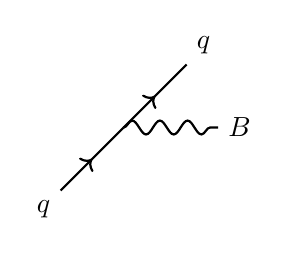
\begin{tikzpicture}[scale=0.8]
\begin{scope}[thick,decoration={
    markings,
    mark=at position 0.5 with {\arrow{>}}}
    ] 
\draw[postaction = {decorate}] (-1,-1) node[below left]{$q$} -- (0,0);
\draw[postaction = {decorate}] (0,0) -- (1,1) node[above right]{$q$};
\end{scope}

\draw[thick, snake it] (0,0) -- (1.5,0) node[right]{$B$};
\end{tikzpicture}}
\qquad
 \subfigure[]{
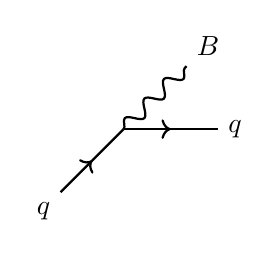
\begin{tikzpicture}[scale=0.8]
\begin{scope}[thick,decoration={
    markings,
    mark=at position 0.5 with {\arrow{>}}}
    ] 
\draw[postaction = {decorate}] (-1,-1) node[below left]{$q$} -- (0,0);
\draw[postaction = {decorate}] (0,0) -- (1.5,0) node[right]{$q$};
\end{scope}

\draw[thick, snake it] (0,0) -- (1,1) node[above right]{$B$};
\end{tikzpicture}}
\qquad
 \subfigure[]{
\begin{tikzpicture}[scale=0.8]
\begin{scope}[thick,decoration={
    markings,
    mark=at position 0.5 with {\arrow{>}}}
    ] 
\draw[postaction = {decorate}] (1,1)  node[above right]{$\bar{q}$}-- (0,0) ;
\draw[postaction = {decorate}] (0,0)  -- (1.5,0) node[right]{$q$};
\end{scope}

\draw[thick, snake it] (-1,-1) node[below left]{$B$} -- (0,0) ;
\end{tikzpicture}}
\qquad
 \subfigure[]{
\begin{tikzpicture}[scale=0.8]
\draw[thick, snake it] (-1,-1) node[below left]{$B$} -- (1,1) node[above right]{$B$};
\end{tikzpicture}}
\caption{The diagrams involving dark photons which contribute to splitting functions. (a), (b), (c), (d) show the contributions to $P_{qq}^{(0,0,1)}(x)$, $P_{Bq}^{(0,0,1)}(x)$, $P_{qB}^{(0,0,1)}(x)$ and $P_{BB}^{(0,0,1)}(x)$, respectively (note at this order, $P_{BB}^{(0,0,1)}(x)$ is proportional to a delta function, $\delta(1-x)$, indicating the lack of possible splitting in this channel).}
\label{fig:splittingfunctions}
\end{figure}

%
The coefficients $P_{ij}^{(0,0,1)}$ can be calculated directly by
finding the most collinearly-divergent parts of the four dark
splitting channels pictured in Fig.~\ref{fig:splittingfunctions}. The only non-zero contributions are given by $ij=qq, qB, Bq$ and $BB$ (the results are the same for antiquarks).
A summary of the calculation is given in App. A of Ref.~\cite{McCullough:2022hzr}; 
however, a detailed calculation is not strictly necessary, since the form
of the interaction Lagrangian Eq.~(\ref{eq:darkphotoninteraction}) is identical
to that of the electromagnetic-hadronic interaction in the SM,
except with a universal coupling $\frac{1}{3}g_B$ to all quarks and antiquarks.
It follows that the splitting function contributions provided by the
dark photon $B$ will be identical (up to a factor of $\frac{1}{9}$, due to
our convention for the universal coupling) to those provided by the
photon $\gamma$; in particular, we can quote the required leading-order
splitting functions by comparing to \cite{Bertone:2015lqa}:
\begin{align}
\label{eq:splittingfunctions}
P_{qq}^{(0,0,1)}(x) &= \frac{1}{9}P_{qq}^{(0,1,0)}(x) = \frac{1+x^2}{9(1-x)_+} + \frac{1}{6} \delta(1-x), \notag\\\notag\\
 P_{BB}^{(0,0,1)}(x) &= \frac{1}{9} P_{\gamma\gamma}^{(0,1,0)}(x)= -\frac{2}{27}\delta(1-x), \notag\\ \\
P_{qB}^{(0,0,1)}(x) &= \frac{1}{9} P_{q\gamma}^{(0,1,0)}(x) = \frac{x^2 + (1-x)^2}{9},\notag\\\notag\\
 P_{Bq}^{(0,0,1)}(x) &= \frac{1}{9} P_{\gamma q}^{(0,1,0)}(x) = \frac{1}{9} \left( \frac{1 + (1-x)^2}{x} \right). \notag
\end{align}
%To solve the modified DGLAP equations~\eqref{eq:basicdglap}, we must
%also specify initial conditions for the dark photon at the initial scale $Q_0 = 1.65\ \text{GeV}$. 
%Given that we consider masses $m_B \in [2,80]$ GeV, we set $B(x,Q^2)
%= 0$ for all $Q < m_B$, and we generate the dark photon PDF dynamically
%at the threshold $Q = m_B$ from PDF evolution, similar to the
%treatment of heavy quarks in the ZM-VFN scheme~\cite{Maltoni:2012pa,Bertone:2017djs}, and the tau
%PDF in~\cite{Bertone:2015lqa}. Hence the dark photon PDF is always
%proportional to the dark photon coupling $\alpha_B$ and to
%$\log(Q^2/m_B^2)$ for $Q>m_B$. 

\subsection{PDF sets with dark photons}
\label{sec:pdf_sets_with_dark_photons}

We have implemented the modified DGLAP equations described in~Sec. \ref{subsec:dglap} in the
public APFEL PDF evolution code~\cite{Bertone:2013vaa}, which is an accurate and flexible code that can be used to perform PDF evolution up to NNLO
in QCD and NLO in QED, using a variety of heavy flavour schemes.
The evolution is performed in $x$-space,\footnote{Rather than Mellin $N$-space, which is an alternative obtained by taking the Mellin transform of the DGLAP equations.} and uses a rotated 
basis of PDFs such that a maximal number of PDF flavour combinations
evolve independently. If we define the following vector of PDFs:
\begin{equation}
\label{eq:singlet}
\vec{q}^S = \begin{pmatrix} g \\ \gamma \\ \Sigma \\ \Delta_{\Sigma} \\ B\end{pmatrix},
\end{equation}
where:
\begin{equation}
\label{eq:singlet2}
\Sigma = \sum_{f=u,d,s,c} (f + \bar{f}), \qquad \Delta_{\Sigma} = \sum_{f=u,c} (f + \bar{f}) - \sum_{f=d,s} (f + \bar{f}),
\end{equation}
then we can choose further independent flavour combinations of PDFs, spanning the
complete space of PDFs, such that all of the remaining flavour combinations' evolution equations decouple;
 this greatly simplifies the computational work. The remaining matrix equation for $\vec{q}^S$ can 
 be shown to take the form:
 \renewcommand{\arraystretch}{0.8}
\begin{equation}
\label{eq:dglapevolution}
\mu_F^2 \frac{\partial \vec{q}^S}{\partial \mu_F^2} = \left(\begin{array}{cccc|c} & & & &  0 \\ & \ddots& \ddots& & 0 \\ & \ddots& \ddots& & P_{q B} \\[1ex] & & & & P_{q B} \\[1ex] \hline 0 & 0 & P_{Bq} & 0 & P_{BB} \end{array}\right) \otimes \vec{q}^S.
\end{equation}
Here, the dots denote the relevant SM matrix, with the quark-quark splitting function corrected with a dark contribution as appropriate. This equation (together with the other decoupled scalar equations) is solved using an adaptive step-size fifth-order Runge-Kutta method, 
as described in~\cite{Bertone:2013vaa}.% and [...].

To solve the modified DGLAP equations~\eqref{eq:basicdglap}, we must
also specify initial conditions for the dark photon;
this is where we make appropriate ans\"{a}tze for the functional form of the dark photon at the initial scale $Q_0 = 1.65\ \text{GeV}$. 
If the mass of the dark photon $m_B$ were less than the scale $Q_0$, we
could postulate a functional form for the initial dark photon PDF
assuming that the dark photon PDF is primarily generated by quark
splitting.
An appropriate initial condition in this case would be given by:
\begin{equation}
\label{eq:lowmassansatz}
B(x,Q_0^2) = \frac{\alpha_B}{2\pi} \log\left( \frac{Q_0^2}{m_B^2} \right) \sum_{j=1}^{n_f} \left(P_{Bq_j} \otimes q_j(x,Q_0^2)+ P_{B\overline{q}_j} \otimes \bar{q}_j(x,Q_0^2) \right).
\end{equation}
On the other hand, our region of interest is $m_B \in [2,80]$ GeV;
in this region, we always have $m_B >
2$ GeV. Thus in our case, we always have $m_B > Q_0$; that is, the mass threshold is always greater than
the initial scale. As a result, we set $B(x,Q^2) = 0$ for all $Q < m_B$ and we generate the dark photon PDF dynamically at the threshold $Q = m_B$ from PDF evolution, similar to the treatment of heavy quarks~\cite{Maltoni:2012pa,Bertone:2017djs}, and the tau PDF in~\cite{Bertone:2015lqa}. 



Using the modified code, we produce a PDF set and a corresponding LHAPDF
grid~\cite{Buckley:2014ana} including dark photons, for each given
value of the dark photon mass and coupling that we consider. 
We focus on the introduction of a dark photon into the evolution of the
{\tt NNPDF3.1luxQED} set~\cite{Bertone:2017bme},\footnote{This
    set will be soon superseded by the PDF set including QED effects
    obtained starting from NNPDF4.0~\cite{NNPDF:2021njg}.} which provides our
SM baseline, namely an NNLO
global PDF analysis of all standard parton flavours together with a photon PDF (the photon
PDF in this set is determined using the state-of-the-art {\tt LUXqed}
method~\cite{Manohar:2017eqh}).\\

\noindent For demonstration purposes, we now proceed to display the key
results from a `dark PDF set' in a particular scenario
that is permitted according to the bounds given in
Ref.~\cite{Ilten:2018crw}, namely:
%two scenarios (both of which are permitted according to the bounds given in~\cite{Ilten:2018crw}):
%\begin{itemize}
%\item \textbf{Scenario I.} The dark photon has mass $m_B = 5\ \text{GeV}$ and coupling $\alpha_B = 10^{-3}$.
%\item \textbf{Scenario II.} The dark photon has mass $m_B = 50\ \text{GeV}$ and coupling $\alpha_B = 3 \times 10^{-3}$.
%\end{itemize}
\begin{equation}
  \label{eq:value}
  m_B = 50\,\, \text{GeV}, \qquad \alpha_B = 3 \times 10^{-3},
\end{equation}
which corresponds to taking $g_B = 1.94 \times 10^{-1}$. As described
above, a massless dark photon is generated dynamically at the threshold $Q = m_B$, and is set
to zero before this threshold is reached. We have chosen a sufficiently
high (admissible) value of the coupling to display the impact
upon PDFs and parton luminosities. 
%
\begin{figure}[hbt]
\centering
\includegraphics[width=0.49\textwidth]{darkphoton_figures/vhigh_dark_photon_comparison_100GeV.pdf}
\includegraphics[width=0.49\textwidth]{darkphoton_figures/vhigh_dark_photon_comparison_1TeV.pdf}
\caption{Comparison of $x\gamma(x,Q^2)$ and $xB(x,Q^2)$ at $Q=100\ \text{GeV}$ (left) and $Q=1\ \text{TeV}$ (right)
for the values of dark photon mass and coupling given in
Eq.~\eqref{eq:value}. The percentage relative 68\% C.L. PDF
uncertainties of the photon and the dark photon are
  displayed in the bottom inset.}
  %The dark photon uncertainty is mostly comparable to the photon uncertainty... \JM{perhaps add more comments here?}}
\label{fig:dark_pdfs}
\end{figure}

In Fig.~\ref{fig:dark_pdfs}, we display both the photon and dark
photon PDFs in our representative dark set (obtained by setting the
dark photon coupling and mass at the values given in
Eq.~\eqref{eq:value}) at the scales $Q = 100\ \text{GeV}$ and $Q=1\ \text{TeV}$,
and show their relative PDF uncertainties. As anticipated, the dark photon PDF features 
the same functional form as the photon PDF (this is to be expected
since the photon and dark photon splitting functions are identical up
to scaling), but its density is smaller since $\alpha_B \lesssim
\alpha$. Furthermore, it can be shown that increasing $\alpha_B$, and also moderately decreasing 
$m_B$, increases the similarity of the dark photon and photon PDFs.
The dark photon uncertainty is mostly comparable to the photon
uncertainty up to $x\sim 0.4$, and then increases faster than the photon
uncertainty. This is due to the dark photon being generated off the
singlet PDF (the sum of all quarks and antiquarks) at its mass
threshold with a rather small coupling; in particular, the dark
photon uncertainty is comparable to the uncertainty of the singlet PDF
scaled by a factor of  $\alpha_B$. This makes it comparable to the
photon PDF uncertainty (for the choice of $\alpha_B$ and $m_B$ of
Eq.~\eqref{eq:value}), except in the large-$x$ region where the singlet PDF uncertainty dramatically increases,
resulting in the dark photon PDF uncertainty to consistently increase up to $\sim10\%$ at
$x\sim 0.6$. We have verified that for larger couplings the
uncertainty increases, as one would expect. 


Now that we have introduced a new parton in the proton, it is 
interesting to ask how much `space' it takes up; this can be quantified
by determining the momentum carried by the dark photon at 
different energy scales. By definition, the momentum fraction carried by any given
parton flavour $f$ at the scale $Q$ is given by:
\begin{equation}
\label{eq:momfraction}
\langle x\rangle_f(Q) := \int\limits_{0}^{1} dx\ xf(x,Q).
\end{equation}
In Table.~\ref{tab:dark_momentum}, we give a comparison between the
momentum carried by the dark photon, the photon and the singlet for
the representative dark PDF
set computed using the values specified in Eq.~\eqref{eq:value}, and
compare them to the baseline SM PDF set, at $Q=100$ GeV and $Q=1$ TeV. 
We observe that the fraction of the proton momentum carried by the
dark photon increases with the scale $Q$, which is to be expected 
by analogy with the photon's behaviour. Depending on the coupling
and the mass of the dark photon, the latter carries up to a fraction
of percent of the proton momentum's fraction at $Q\approx1\
\text{TeV}$. 
\begin{table}[tb]
\centering
\begin{tabularx}{\textwidth}{X|C{1.8cm}C{1.8cm}C{1.8cm}C{1.8cm}}
\toprule
$\langle x\rangle_f(Q=100$ GeV) & $f=\Sigma$ & $f=\gamma$ & $f=B$ \\
\midrule
Baseline &  50.23\% &  0.4241\% & 0\% \\
Dark set & 50.17\% & 0.4241\% &0.03214\%  \\
\midrule
$\langle x\rangle_f(Q=1$ TeV) & $f=\Sigma$ & $f=\gamma$ & $f=B$ \\
\midrule
Baseline &  48.36\% &  0.5279\% & 0\% \\
Dark set & 48.12\% &  0.5275\% & 0.1357\%  \\
\bottomrule
\end{tabularx}
%\includegraphics[width=0.7\textwidth]{vhigh_momentum_distribution_log.pdf}
\caption{A comparison between the momentum fraction percentage carried by the
  singlet $\Sigma$, the photon $\gamma$, and the dark photon $B$ at $Q=100$ GeV and $Q=1$ TeV,
  for the baseline SM set and the dark
  PDF set, obtained with the photon coupling and mass given in Eq.~\eqref{eq:value}. The momentum
fraction is computed on the central replica in each case. }
\label{tab:dark_momentum}
\end{table}


Crucially, the presence of a dark photon in the DGLAP equations also
modifies the evolution of all other flavours of PDFs due to the
coupling of the PDFs via the modified DGLAP equations
Eq.~(\ref{eq:basicdglap}).
We expect that the modification of the quark and antiquark 
flavours is strongest, as the dark photon is directly coupled to
them. We also anticipate a modification to the gluon and photon
PDFs, but these will be second order effects, so we expect that they
will be smaller in comparison. Moreover, the density of each of the
flavours should reduce, as the new dark photon `takes up space' in the
proton which was previously occupied by the quark flavours.
\begin{figure}[tb]
\centering
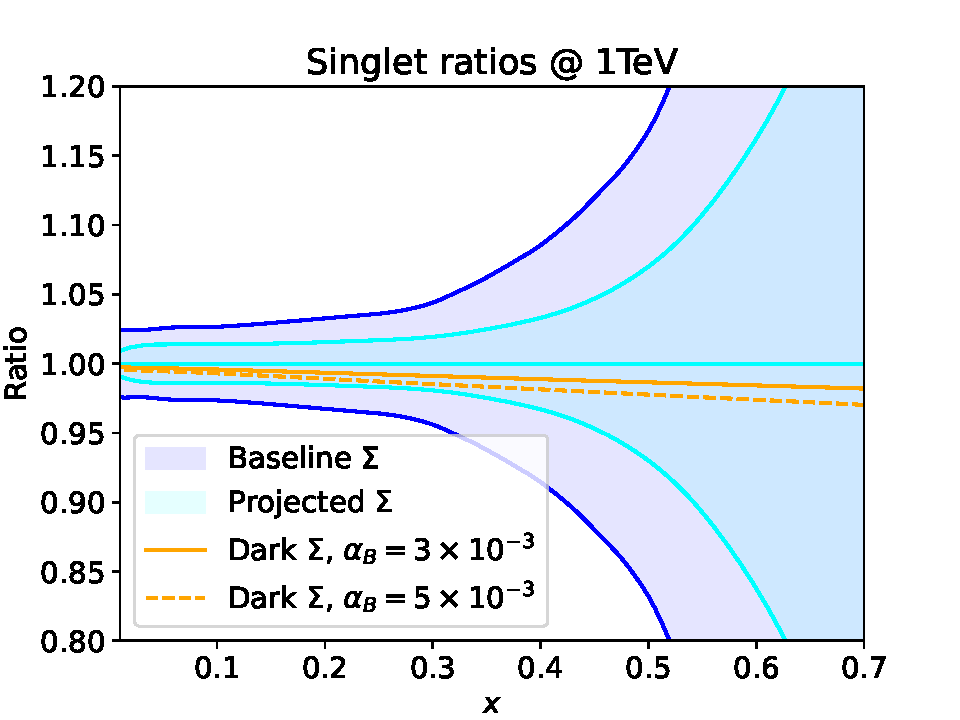
\includegraphics[width=0.49\textwidth]{darkphoton_figures/singlet_ratios_1TeV.pdf}
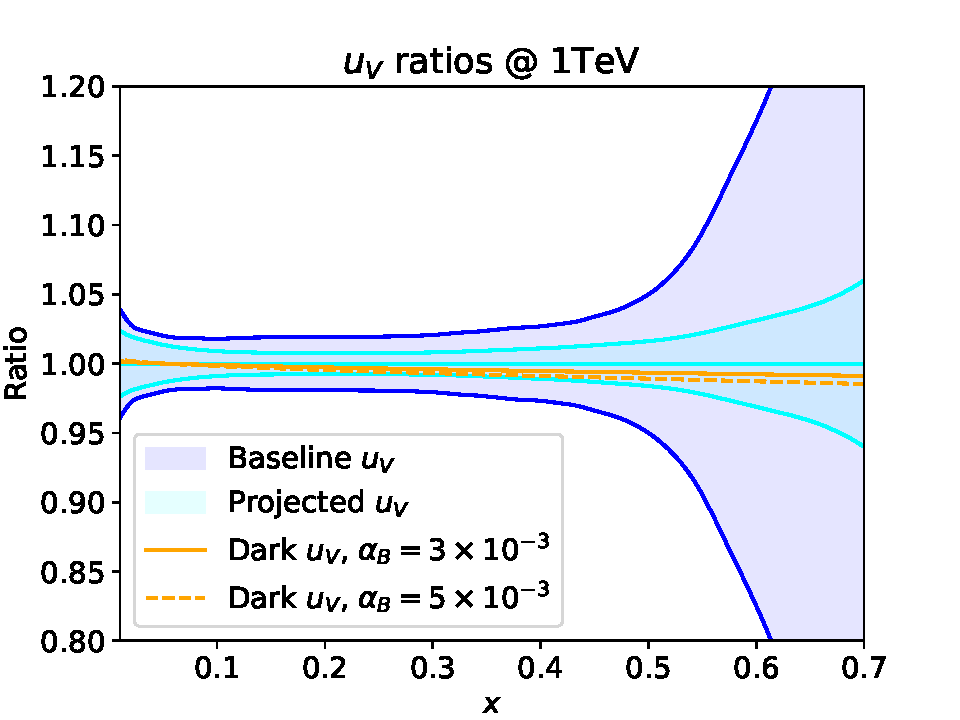
\includegraphics[width=0.49\textwidth]{darkphoton_figures/uvalence_ratios_1TeV.pdf}
\caption{In solid orange, the ratio between the central singlet PDF $\Sigma$ (left) and central $u$-valence
  PDF (right), drawn from the dark benchmark scenario in Eq.~\eqref{eq:value}, 
  to the baseline SM central replica at $Q = 1\
  \text{TeV}$. In dashed orange, the same ratios but between the SM baseline and a dark PDF set
  produced using $m_B = 50\ \text{GeV}, \alpha_B = 5 \times 10^{-3}$. In each case, the uncertainty bands
  represent the 68\% C.L. PDF uncertainties of the baseline set (in blue) 
  and the projected PDF uncertainties at the HL-LHC, determined
  from Ref.~\cite{Khalek:2018} (in light blue). The deviation when $\alpha_B = 5 \times 10^{-3}$ approaches
  the boundary of the projected HL-LHC uncertainty bands, consistent with the behaviour we see in Fig.~\ref{fig:14tevlumis} later; increasing $\alpha_B$ (and also to a milder extent, decreasing $m_B$) pushes the deviation outside of projected HL-LHC uncertainty bands.
  See the main text for more details.}
\label{fig:ratio_quarks}
\end{figure}
Results are shown in Fig.~\ref{fig:ratio_quarks}, in which the ratio
between the central value of the dark-photon modified singlet
($u$-valence) PDF and the central value of the baseline singlet
($u$-valence) PDF are displayed and compared to the current 68\% C.L. PDF
uncertainty. 

We observe
that the modification of the singlet becomes visible at about $x\sim 0.2$ and
reaches 3\% at larger values of $x\sim 0.5$. This is well within the
68\% C.L. uncertainty of the singlet PDF from the baseline {\tt
  NNPDF3.1luxQED} NNLO set. However, thanks to the inclusion of a vast
number of new datasets and the increased precision of the methodology
used in global PDF analysis, the recent {\tt NNPDF4.0} NNLO
set~\cite{NNPDF:2021njg} 
displays significantly smaller large-$x$ uncertainty. Such a
decrease in PDF uncertainties goes in the direction indicated by the
dedicated study on how PDF
uncertainties will decrease in future, thanks to the inclusion of precise
HL-LHC measurements~\cite{Khalek:2018}. In particular, to give an indication
of how the modification of PDFs due to the presence of a dark photon might
come into tension with decreasing PDF uncertainties during the HL-LHC phase, 
we display the projected 68\% PDF uncertainties at
the HL-LHC determined in the `optimistic' scenario, Scenario 3, of Ref.~\cite{Khalek:2018}.
In this case, should PDF uncertainties decrease to the
level predicted by Ref.~\cite{Khalek:2018}, the distorted singlet PDF approaches the edge of the
projected PDF uncertainty at $x\sim \,0.1-0.3$ region, for the values given
in Eq.~\eqref{eq:value}. This is particularly relevant for the
analysis that we present in the next section. 




\newpage
\section{Phenomenological implications and projected bounds}
\label{sec:dark_pheno}

In this section we review the existing constraints on the dark photon.
Subsequently, in order to assess the impact of a non-zero dark photon
parton density on physical observables, we plot the parton luminosities
when the dark photon is included, as compared to our baseline SM set. 
We compare the predicted deviations with the current PDF
uncertainties and with the projected PDF uncertainties at the HL-LHC.
Finally, we motivate and present an analysis of projected HL-LHC Drell-Yan data 
and compare the maximal sensitivity we can achieve to the existing
bounds derived in the literature.

\subsection{Review of existing constraints on the dark photon}
\label{sec:existingconstraints}
To appreciate the utility of the dark photon PDF at colliders, we may compare to alternative probes.  Recent works considering this class of baryonic dark photon models include \cite{Dobrescu:2014fca,Dror:2017ehi,Ismail:2017fgq,Dror:2018wfl,Ilten:2018crw,Dobrescu:2021vak}.  There are a variety of competing constraints on this scenario, of varying theoretical robustness.

One class of constraints, first considered in detail in
\cite{Dobrescu:2014fca}, is theoretical and concerns the mixed $\text{U}(1)_B-$EW anomalies.  Suppose we envisage that the UV-completion of the model Eq.~\eqref{eq:darkphotoninteraction} is perturbative with $\text{U}(1)_B$ linearly realised.  In that case, the mixed anomaly must be UV-completed by some fermions with electroweak charges.  Early studies of the classes of fermions that can achieve this include \cite{Duerr:2013dza,FileviezPerez:2014lnj}.\footnote{Note also that the required fermions could serve as potential dark matter candidates, as discussed in \cite{FileviezPerez:2019jju,Perez:2020jyg,Perez:2021rbo}.}   In this perturbative UV-completion they will obtain their mass from spontaneous $\text{U}(1)_B$-breaking.  As a result, they will be coupled to the longitudinal mode of $B$ and an additional Higgs-like scalar with a Yukawa coupling $\lambda \propto M_F/v_B$, where $M_F$ is the fermion mass, $v_B$ is the $\text{U}(1)_B$-breaking expectation value, and we have assumed three sets of fermions with the same charge ($1/3$) as the left-handed fermions, for simplicity.  On the other hand we have $g_B  \propto M_B/v_B$ following from the charge and symmetry-breaking vacuum expectation value.  As a result, we expect:
\begin{equation}
g_B \approx \frac{2 \lambda}{3} \frac{M_B}{M_F},
\end{equation}
where the precise numerical factors are taken from \cite{Dobrescu:2014fca}.  Thus, requiring perturbativity $\lambda \lesssim 4 \pi$ implies an upper bound on $g_B$, where the factor $1/3$ follows from the fact that each family of fermions is in triplicate to mirror the QCD multiplicity of the SM quarks.  This limit is shown as a dashed line in Fig.~\ref{fig:limits} where we have taken $M_F\geq 90$ GeV for the electroweak-charged fermions. 

However, a number of implicit assumptions have been made which can weaken upon further inspection.  To see this, consider cancelling the anomaly with $N$ copies of the above class of fermions.  In this case the limit becomes:
\begin{equation}
g_B \lesssim \frac{8 \pi}{3} \frac{N}{3} \frac{M_B}{M_F} ~~.
\end{equation}
Hence we see that this theoretical limit makes not only the assumption of a weakly-coupled UV-completion, but also depends on assumptions of minimality of the UV completion as well.  As a result, while this limit does guide the eye as to the nature of the UV-completion, it cannot be considered a strong theoretical limit on the model parameters.

Another constraint which is very relevant in some UV-completions concerns Higgs boson decays.  In some UV-completions the radial mode of spontaneous symmetry breaking may mix with the Higgs boson, giving rise to Higgs decays to $B$'s.  Depending on the magnitude of the mixing angle the corresponding constraints can be strong, as demonstrated in \cite{Perez:2020izb}.  Care must be taken to consider these processes in any specific UV-completion, however as the rates depend strongly on the details of the UV-completion we do not include them in our analysis here, which is focussed on the irreducible model-independent IR physics.

The only truly model-independent theoretical limit comes from considering the scale at which the validity of the IR theory itself breaks down.  Given that the quark interactions are vector-like there is no possibility of tree-level unitarity violation in quark scattering mediated by $B$, thus we must look to quantum effects.  In this case the mixed-anomaly becomes relevant and renders the theory non-unitary unless \cite{Preskill:1990fr}:
\begin{equation}
g_B \lesssim \frac{(4 \pi)^2}{3 \alpha_W} \frac{M_B}{M_\Lambda} ~~,
\end{equation}
where $\alpha_W$ is the $\text{SU}(2)$ fine structure constant at the electroweak scale and $M_\Lambda $ is the energy scale at which the theory becomes strongly coupled.  Numerically this is
\begin{equation}
g_B \lesssim \frac{3M_B}{5 \text{ GeV}} \frac{10 \text{ TeV}}{M_\Lambda} ~~,
\end{equation}
which is too weak to be relevant for our purposes.  As a result we conclude that the effective theory considered here is valid throughout the energy scales under investigation. However, we note that, as shown in
\cite{Dobrescu:2021vak}, the mixing with the $Z$-boson is sensitive to
the details of the UV-completion; for this reason we restrict the mass range under
investigation to $m_B \leq 80\ \text{GeV}$, above which these UV-dependent effects can be important.  %One could impose \ae sthetic constraints on the UV completion in order to constrain the parameters of the IR theory, however in this case the model-dependence of the constraint must be kept in mind.

There are three relevant classes of experimental constraints.  The first
concerns the exotic $Z$-boson decays $Z\to B\gamma$.  These constraints
were calculated in \cite{Dror:2017ehi} based on the LEP analysis for
$Z\to H\gamma$, $H\to$hadrons~\cite{L3:1996dmt}.\footnote{Note that
  this reference does not appear in~\cite{Dror:2017ehi}, but instead
  in~\cite{L3:1991kow,L3:1992kcg}, however the authors of
  \cite{Dror:2017ehi} have confirmed that the limits follow from a
  recasting of \cite{L3:1996dmt}.} This limit, relevant to the higher
mass range, is shown in red in Fig.~\ref{fig:limits}.  The second
class of constraints at lower masses concerns exotic $\Upsilon$ decays
\cite{Carone:1994aa,Aranda:1998fr}, where the constraint is dominated
by limits on $\Upsilon(1S)\to 2$ jets \cite{ARGUS:1986nzm}, shown in
blue in Fig.~\ref{fig:limits}. Finally, there are additional searches for
hadronically decaying resonances at hadron colliders
\cite{Dobrescu:2013cmh,Shimmin:2016vlc,ATLAS:2019itm,Dobrescu:2021vak}.
The strongest are from CMS $B+$ISR searches
\cite{CMS:2019xai,CMS:2019emo}, shown in yellow in
Fig.~\ref{fig:limits}. 

\subsection{Effects of the dark photon on parton luminosities}
In Sec.~\ref{subsec:dglap}, we showed that the presence of a dark photon modifies
all other flavours of PDFs via the mixing associated with the
DGLAP evolution equations, with a modification that is proportional to
$\alpha_B$ and the logarithm of $m_B$. 
In order to assess the impact of a dark photon
parton density on physical observables, and thus extract the 
sensitivity that the LHC can achieve on the
parameters of the model, in the following subsection
we compare the size of the dark parton luminosities to luminosities
involving the other partons, and assess the impact of the dark photon
on the dominant partonic channels.

%Given that in the computation of the cross sections of hadron-collider processes, PDF contributions
%factorise in the form of, it
%is useful to study the behaviour of the parton luminosities of the different initial states, by
%including also the dark photon. %{\color{red} Text here very similar to lepton PDF paper.}
Parton luminosities are doubly differential quantities defined as:
\begin{equation}
\frac{d{\cal L}_{ij}}{dyd\tau}=f_i(x_1,Q^2)f_j(x_2,Q^2)\qquad x_{1,2}=\sqrt{\tau}\exp(\pm
y)\qquad \tau=\frac{M_X^2}{S},
\end{equation}
where $S$ is the squared centre-of-mass energy of the hadronic collision, $M_X$ is the invariant mass
of the partonic final state, $y$ is the rapidity of the partonic final state, and 
$f_i(x,Q^2)$ is the PDF of the $i$th parton evaluated at the
scale $Q$. Different choices for $Q$ can be adopted in order to improve predictions
of a particular process and/or distribution.
At the level of pure luminosities, without the convolution with
any specific matrix element, the factorisation scale can be naturally
set to $Q = M_X$. For plotting purposes, it is useful to define the
$M_X$-differential luminosities, given by:
\begin{equation}
  \label{eq:lumidef}
\Phi_{ij}(M_X) \,=\,\frac{d{\cal L}_{ij}}{dM_X^2}=\frac{1}{S}\,\int\limits_{M_X^2/S}^1
\frac{dx}{x}\ f_i(x,M_X^2)f_j\left(\frac{M_X^2}{xS},M_X^2\right).
\end{equation}

%
\begin{figure}[tb]
\centering
% \subfigure[]{
% \includegraphics[scale=0.43]{high_BB_gmgm_luminosity_14TeV.pdf}}
% \quad
%  \subfigure[]{
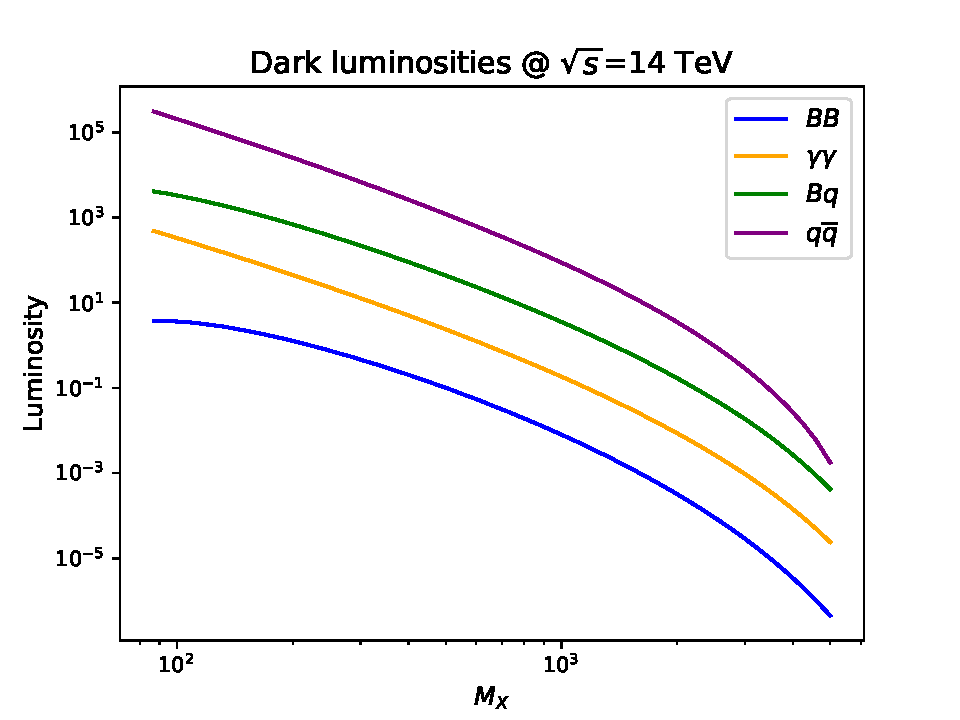
\includegraphics[width=0.7\textwidth]{darkphoton_figures/vhigh_BB_gmgm_luminosity_14TeV.pdf}
\caption{Comparison of the absolute value of the $\Phi_{BB}$,
  $\Phi_{qB}$ central luminosities and the $\Phi_{\gamma\gamma}$  and
  $\Phi_{qq}$ central luminosities as a function of the invariant mass $M_X$
  at the centre of mass energy $\sqrt{s} = 14\ \text{TeV}$ for the dark PDF set obtained with 
 the dark photon coupling and mass set in Eq.~\eqref{eq:value}.% , in
  % Scenario I and II respectively. Note that in Scenario II, the gradient of
  % $\Phi_{BB}$ and $\Phi_{Bq}$ plateaus as we approach $M_X = 100\ \text{GeV}$ from 
  % above; this is to be expected, since these luminosities vanish for $M_X \leq 50\ \text{GeV}$,
  % and numerical instability increases in their computation as we approach this mass threshold.
}
\label{fig:lowdarkmass}
\end{figure}
%
We first compare the size and the $M_X$-dependence of the different
parton luminosities in the candidate dark PDF set obtained by setting the mass and the coupling to the
values indicated in Eq.~\eqref{eq:value}. In Fig.~\ref{fig:lowdarkmass} we plot $\Phi_{BB},
\Phi_{Bq}$ as compared to $\Phi_{q\bar{q}}$,
$\Phi_{\gamma\gamma}$. We
observe that, while the $BB$ channel is suppressed by two powers of
the dark coupling, and its size never exceeds more than a fraction of a percent of the
$q\bar{q}$ luminosity, the $Bq$ channel grows from about 2\% of the
$q\bar{q}$ luminosity at $M_X\sim$ 1 TeV to about 8\% of the
$q\bar{q}$ luminosity at larger values of the invariant mass. Its
contribution exceeds that of $\gamma\gamma$ scattering by one order of magnitude. 

\begin{figure}[bht]
\centering
% \subfigure[]{
% \includegraphics[scale=0.43]{high_uubar_luminosity_14TeV.pdf}}
% \quad
%  \subfigure[]{
% \includegraphics[scale=0.43]{vhigh_uubar_luminosity_14TeV.pdf}}
% %
 \subfigure[$m_B=50\ \text{GeV}, \alpha_B = 3 \times 10^{-3}$]{
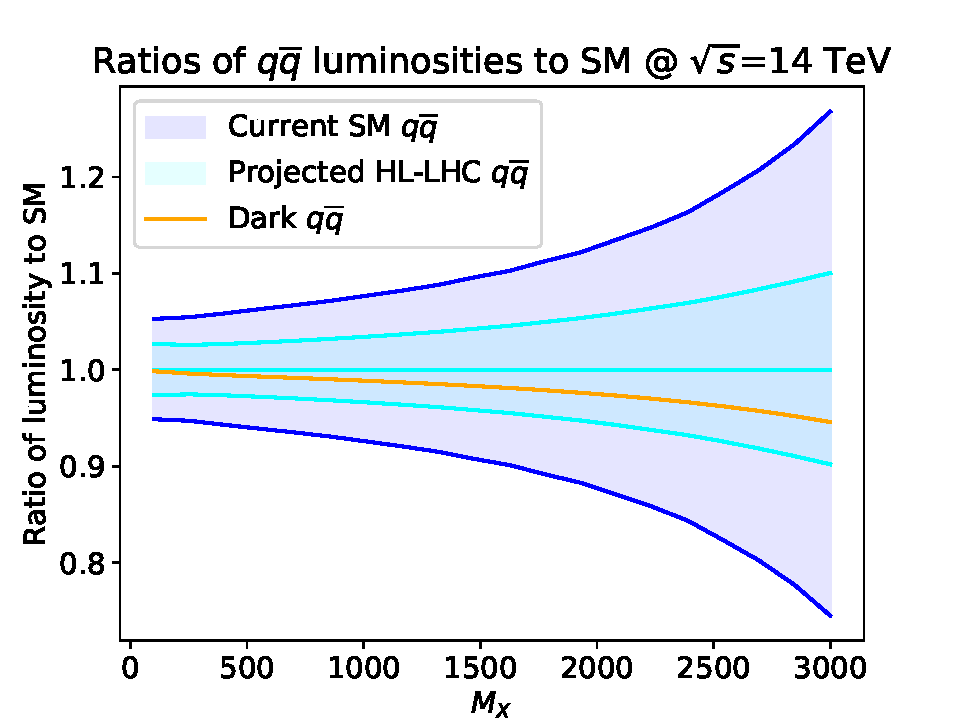
\includegraphics[scale=0.43]{darkphoton_figures/vhigh_qqbar_luminosity_14TeV.pdf}
}
\quad
 \subfigure[$m_B=50\ \text{GeV}, \alpha_B = 5 \times 10^{-3}$]{
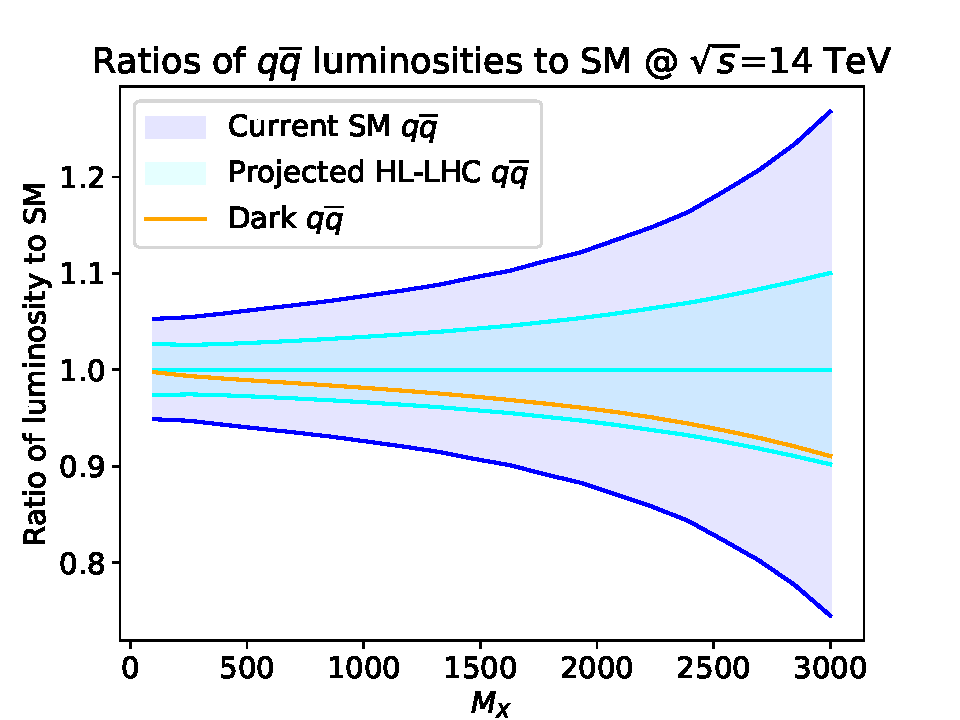
\includegraphics[scale=0.43]{darkphoton_figures/mB_50_alphaB_5e-3_qqbar_luminosity_14TeV.pdf}
}
\quad
  \subfigure[$m_B=5\ \text{GeV}, \alpha_B = 3 \times 10^{-3}$]{
 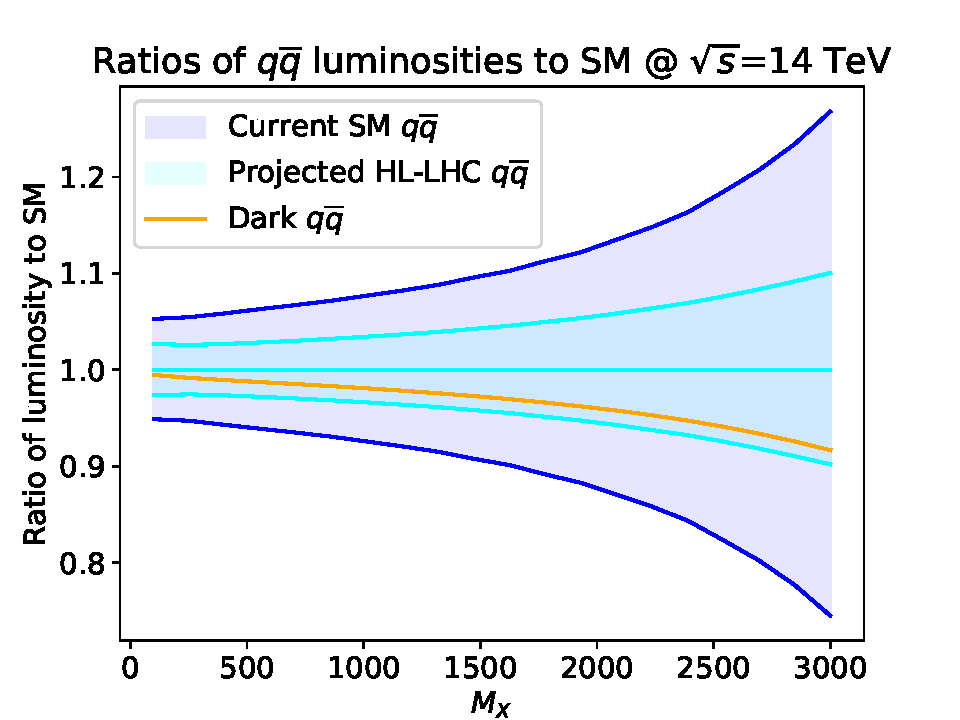
\includegraphics[scale=0.43]{darkphoton_figures/mB_5_alphaB_3e-3_qqbar_luminosity_14TeV.pdf}}
 \quad
  \subfigure[$m_B=5\ \text{GeV}, \alpha_B = 5 \times 10^{-3}$]{
 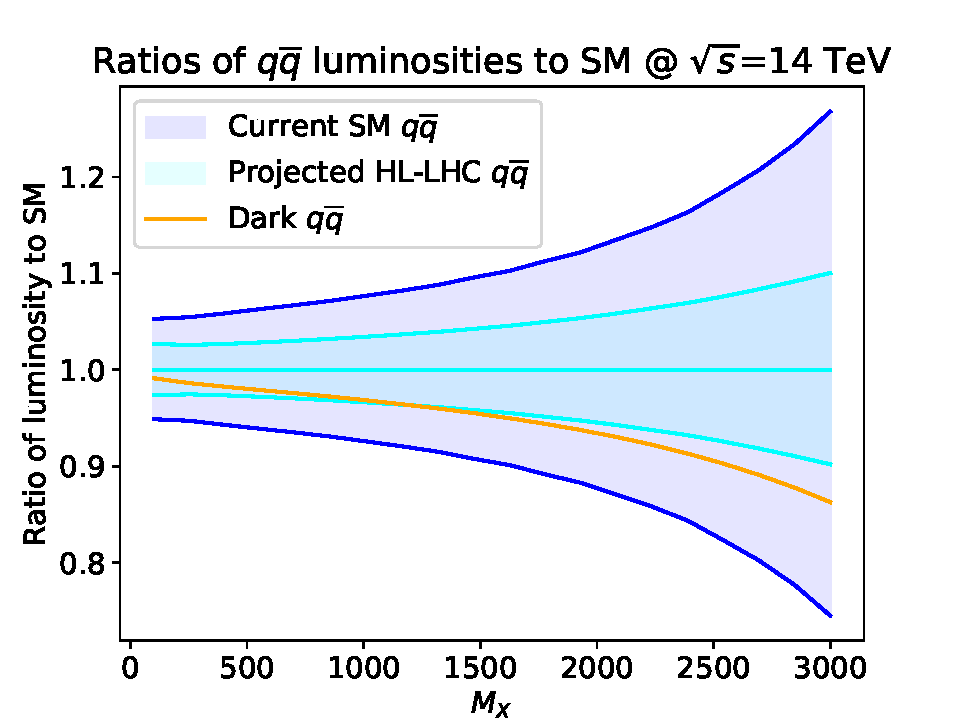
\includegraphics[scale=0.43]{darkphoton_figures/mB_5_alphaB_5e-3_qqbar_luminosity_14TeV.pdf}}
 %
\caption{The ratio $\Phi_{q\bar{q}}^{\text{Dark}}/\Phi_{q\bar{q}}^{\text{SM}}$ for
  % each of the quark flavours $q = u, d$ and
  the total quark-anti-quark luminosity, at the centre of mass energy
  $\sqrt{S} = 14\ \text{TeV}$ for the values of mass and coupling
  indicated under each panel. 
  In each panel, the dark blue bands correspond to the current PDF
  uncertainty, while the light blue bands show the expected uncertainty on the
  PDF luminosity at the HL-LHC. See main text for more details.}
\label{fig:14tevlumis}
\end{figure}
%
We now turn to assess the change in the other luminosities, as a result of the
inclusion of a non-zero dark photon parton density.
In Fig.~\ref{fig:14tevlumis} we display the ratio of the dark-photon
modified quark-antiquark integrated luminosity
$\Phi_{q\bar{q}}^{\text{Dark}}$ with the baseline one, $\Phi_{q\bar{q}}^{\text{SM}}$ at the centre of mass energy
  $\sqrt{S} = 14\ \text{TeV}$, for different values of the $\alpha_B$
  and $m_B$ parameters, starting from our benchmark values, Eq.~\eqref{eq:value}.
  In each figure, the dark blue band corresponds the 68\% C.L. PDF
  uncertainty of the NNLO baseline {\tt NNPDF3.1luxQED} set, while the
  green bands show the projected PDF uncertainty on the
  parton luminosity at the HL-LHC; this estimate for the uncertainty
  on the PDF luminosity is obtained from the `optimistic' scenario, Scenario 3,
  analysed in \cite{Khalek:2018}, as above. 
  %
%  To compute the projected reduction in the
%  PDF uncertainty at the HL-LHC, we take the ratio of the 68\% C.L. 
%  relative uncertainties of the luminosity computed using the public {\tt
%    PDF4LHC15\_nnlo\_hllhc\_scen3}  PDF set associated with the
%  optimistic scenario released alongside
%  Ref.~\cite{Khalek:2018} and those computed with the reference set in
%  the projection study, namely the {\tt PDF4LHC15} PDF
%  set~\cite{Butterworth:2015oua}. We then multiply the 68\% C.L. PDF
%  uncertainty of the NNLO baseline by the ratio to obtain the
%  projected PDF uncertainty at the LHC. 
  Starting from the values of Eq.~\eqref{eq:value}, we observe that
  the deviation in the $q\bar{q}$ luminosity due to the presence of
  the dark photon is significant compared to the size of the
  projected PDF uncertainties at the HL-LHC. Decreasing the mass of
  the dark photon by a factor of 10 increases the impact of the dark
  photon on $q\bar{q}$ initiated observables, while increasing the
  coupling by less than a factor of 2 brings the luminosity beyond the
  edge of the 68\% C.L. error bands. %The appreciable deviation between
 % the dark luminosity and the projected uncertainties on the baseline
  %SM luminosities encourage the phenomenological study in the sequel.

Crucially, the effect of the dark photon is much larger in the $q\bar{q}$-initiated processes than in
any of the other channels, including $qq$, $qg$ and $gg$. This motivates the study of the high-mass Drell-Yan tails that we put
forward in the following section. 


\subsection{Constraints from precise measurements
  of high-energy Drell-Yan tails}
  \label{subsec:dark_constraints}

Given that the $q\bar{q}$ channel is the most affected by the presence of a non-zero dark photon parton density, in this
study we focus on precise measurements of the high-mass Drell-Yan
tails at the HL-LHC. It is important to note that these projected data are not
included in the fit of the input PDF set used as a baseline,
otherwise, as was explicitly shown in ~\cite{Carrazza:2019sec,Greljo:2021kvv,Iranipour:2022iak}, the interplay between the fit of the
new physics parameters and the fit of the PDF parametrisation at the
initial scale might distort the results. 

To generate the HL-LHC pseudodata for neutral-current
high-mass Drell-Yan cross sections at $\sqrt{S}=14$ TeV, we follow the procedure of~\cite{Greljo:2021kvv}.
Namely, we adopt as reference the CMS  measurement at 13 TeV~\cite{CMS:2018mdl} based on $\mathcal{L}=2.8$ fb$^{-1}$.
%
The dilepton invariant mass distribution $m_{\ell\ell}$ is evaluated using the same selection
and acceptance cuts of~\cite{CMS:2018mdl}, but now with an extended
binning in $m_{\ell\ell}$ to account for the increase in luminosity.
%
We assume equal cuts for electrons and muons, and impose $|\eta_\ell|\le 2.4$,
$p_T^{\rm lead}\ge 20$ GeV, and $p_T^{\rm sublead}\ge 15$ GeV for the two
leading charged leptons of the event.
We restrict ourselves to  events with $m_{\ell\ell}$ greater than $500$ GeV, so that 
the total experimental uncertainty is not limited by our modelling
of the expected systematic errors, by making our projections unreliable.
%
To choose the binning, we require that the expected number of events per bin
is bigger than 30 to ensure the applicability of Gaussian statistics.
%
Taking into account these considerations, our choice of binning
for the $m_{\ell\ell}$ distributions at the HL-LHC both in the muon and electron channels 
are displayed in Fig.~\ref{fig:data-theory} with the highest energy bins reaching $m_{\ell\ell}\simeq 4 $ TeV.
In total, we have two invariant mass distributions of 12 bins each, one in the electron and one in the muon channels.

Concerning uncertainties, in Ref.~\cite{Greljo:2021kvv} this data is produced by assuming that the HL-LHC phase will
operate with a total integrated luminosity of $\mathcal{L} = 6\ \text{ab}^{-1}$
(from the combination of ATLAS and CMS, which provide ${\cal L}=3 \,{\rm ab}^{-1}$ each),
and also assuming a five-fold reduction in systematic uncertainty
compared to ~\cite{CMS:2018mdl}. 
We regard this scenario as {\it optimistic} in this chapter; we also
manipulated the projected data so that it reflected a more {\it
  conservative} possibility, where the total integrated luminosity of
the high-mass Drell-Yan tail measurements is $\mathcal{L} = 3\
\text{ab}^{-1}$ (say, for example, they are made available only by
either ATLAS or CMS) and with a two-fold (rather than a five-fold) reduction in systematic uncertainties.

For these projections, the reference theory is the SM, with
theoretical predictions evaluated at NNLO in QCD including full 
NLO EW corrections (including in particular the photon-initiated
contributions); note, however, that the Drell-Yan production has been recently computed at
N${}^3$LO in QCD~\cite{Duhr:2020seh,Duhr:2021vwj}. In the kinematical
region that is explored by our HL-LHC projections ($m_{\ell\ell}>500$
GeV), the perturbative convergence of the series is good and
the N${}^3$LO computation is included within the NNLO prediction, with
missing higher order uncertainty going from about 1\% to a fraction of
a percent. Given the good perturbative convergence of
the matrix element calculation, and the absence of N${}^3$LO PDFs that match
the accuracy of the N${}^3$LO computation of the matrix element, we use the NNLO QCD and NLO EW accuracy of our calculations, both for the SM
baseline and for the dark-photon modified PDF set that we use to
compute the maximal sensitivity to the dark photon parameters. 

The central PDF set used as an input to generate the theoretical prediction is the SM baseline
that we use throughout the paper, namely the NNLO {\tt NNPDF3.1luxQED} set.
The percentage statistical and systematic uncertainties on the HL-LHC pseudodata are then estimated as follows.
Let us denote by  $\sigma^{\rm th}_{i}$ the theoretical prediction for the
DY cross-section from the \texttt{luXQED} set, including all relevant selection cuts
as well as the leptonic branching fractions.
%
The expected number of events in this bin and the associated (relative)
statistical uncertainty $\delta_i^{\rm stat}$ are given by 
\begin{equation}
  N_{i}^{\rm th}= \sigma^{\rm th}_{i}\times \mathcal{L} \,, \quad \delta_i^{\rm stat}\equiv
  \frac{\left( \delta N_{i}\right)_{\rm stat}}{N_{i}^{\rm th}} = \frac{1}{\sqrt{N_{i}^{\rm th}}} \, .
\end{equation}
Note that this bin-by-bin relative statistical uncertainty is the same both at the level
of number of events and at the level of fiducial cross sections.

The HL-LHC systematic uncertainties are also estimated from the same reference
measurements.
%
If $\delta_{i,j}^{\rm sys}$ denotes the $j^{\rm th}$ relative systematic uncertainty
associated to the $i^{\rm th}$ bin of the reference
measurement, and if this bin contains $N_i^{\rm th}$ events,
then for our projections we assume that the same systematic error
associated to a bin with a similar number of expected events will be given by 
$f_{{\rm red},j}\delta_{i,j}^{\rm sys}$, where $f_{{\rm red},j}$
is the expected reduction in systematic errors foreseen at the HL-LHC (we take the reduction factor to be $0.2$ in the \textit{optimistic scenario} and $0.5$ in the \textit{conservative scenario}).
%
This assumption is justified since most systematic errors improve with the sample size
thanks to {\it e.g.} better calibration.

Adding in quadrature systematic uncertainties with the statistical error,
the total relative uncertainty for the $i$th bin of our HL-LHC projections
is:
\begin{equation}
\delta_{{\rm tot},i}^{\rm exp} = \left( \left( \delta_i^{\rm stat}\right)^2 + \sum_{j=1}^{n_{\rm sys}}
\left( f_{{\rm red},j}\delta_{i,j}^{\rm sys} \right)^2\right)^{1/2} \, ,
\end{equation}
where $n_{\rm sys}$ indicates the number of systematic error sources.

The final central values for the HL-LHC pseudodata are then generated
by fluctuating the reference theory prediction by the expected total experimental
uncertainty, namely
\begin{equation}
  \label{eq:hllhc}
\sigma^{\rm hllhc}_{i} \equiv \sigma^{\rm th}_{i} \left( 1+ \lambda
  \delta_{\cal L}^{\rm exp} +  r_i\delta_{{\rm tot},i}^{\rm exp}   \right) \, , \qquad i=1,\ldots,n_{\rm bin} \, ,
\end{equation}
where $\lambda,r_i$ are univariate Gaussian random numbers, $\delta_{{\rm tot},i}^{\rm exp}$
is the total (relative) experimental uncertainty corresponding to this
specific bin
(excluding the luminosity and normalisation uncertainties), and $\delta_{\cal L}^{\rm exp}$
is the luminosity uncertainty, which is fully correlated amongst all
the pseudodata bins of the same experiment. We take this luminosity uncertainty to be
$\delta_{\cal L}^{\rm exp}=1.5$\%  for both ATLAS and CMS, as done in~\cite{Khalek:2018}.

To obtain bounds on the dark photon mass and coupling, we select a grid of benchmark
points $(m_B, \alpha_B)$ in the dark photon parameter space; our scan consists of $21$ points, distributed as a rectangular grid
with masses $m_B = 2, 5, 8, 10, 20, 50, 80\ \text{GeV}$ and couplings
$\alpha_B = 10^{-3}, 2\times10^{-3}, 3 \times 10^{-3}$. We then construct dark PDF sets at each 
of these benchmark points (thus a total of $21$ PDF sets, in each case including quarks, antiquarks, the gluon, the photon and the dark photon PDFs), using the 
appropriate values of $m_B, \alpha_B$, and hence
compute theoretical predictions in both the \textit{optimistic} and \textit{conservative} scenarios at each grid point. The predictions
are produced assuming that the primary contribution comes from the
$q\bar{q}$ channel; in particular, we note that the partonic diagrams that include a dark
photon in the initial state (such as $Bq\to \bar{q}l^+l^-$ or $B\bar{q}\to
ql^+l^-$) are suppressed by two powers of $\alpha_B$, one from the
dark photon PDF and one from the matrix element, and therefore are
suppressed beyond the accuracy of our calculation. 

\begin{figure}
\centering
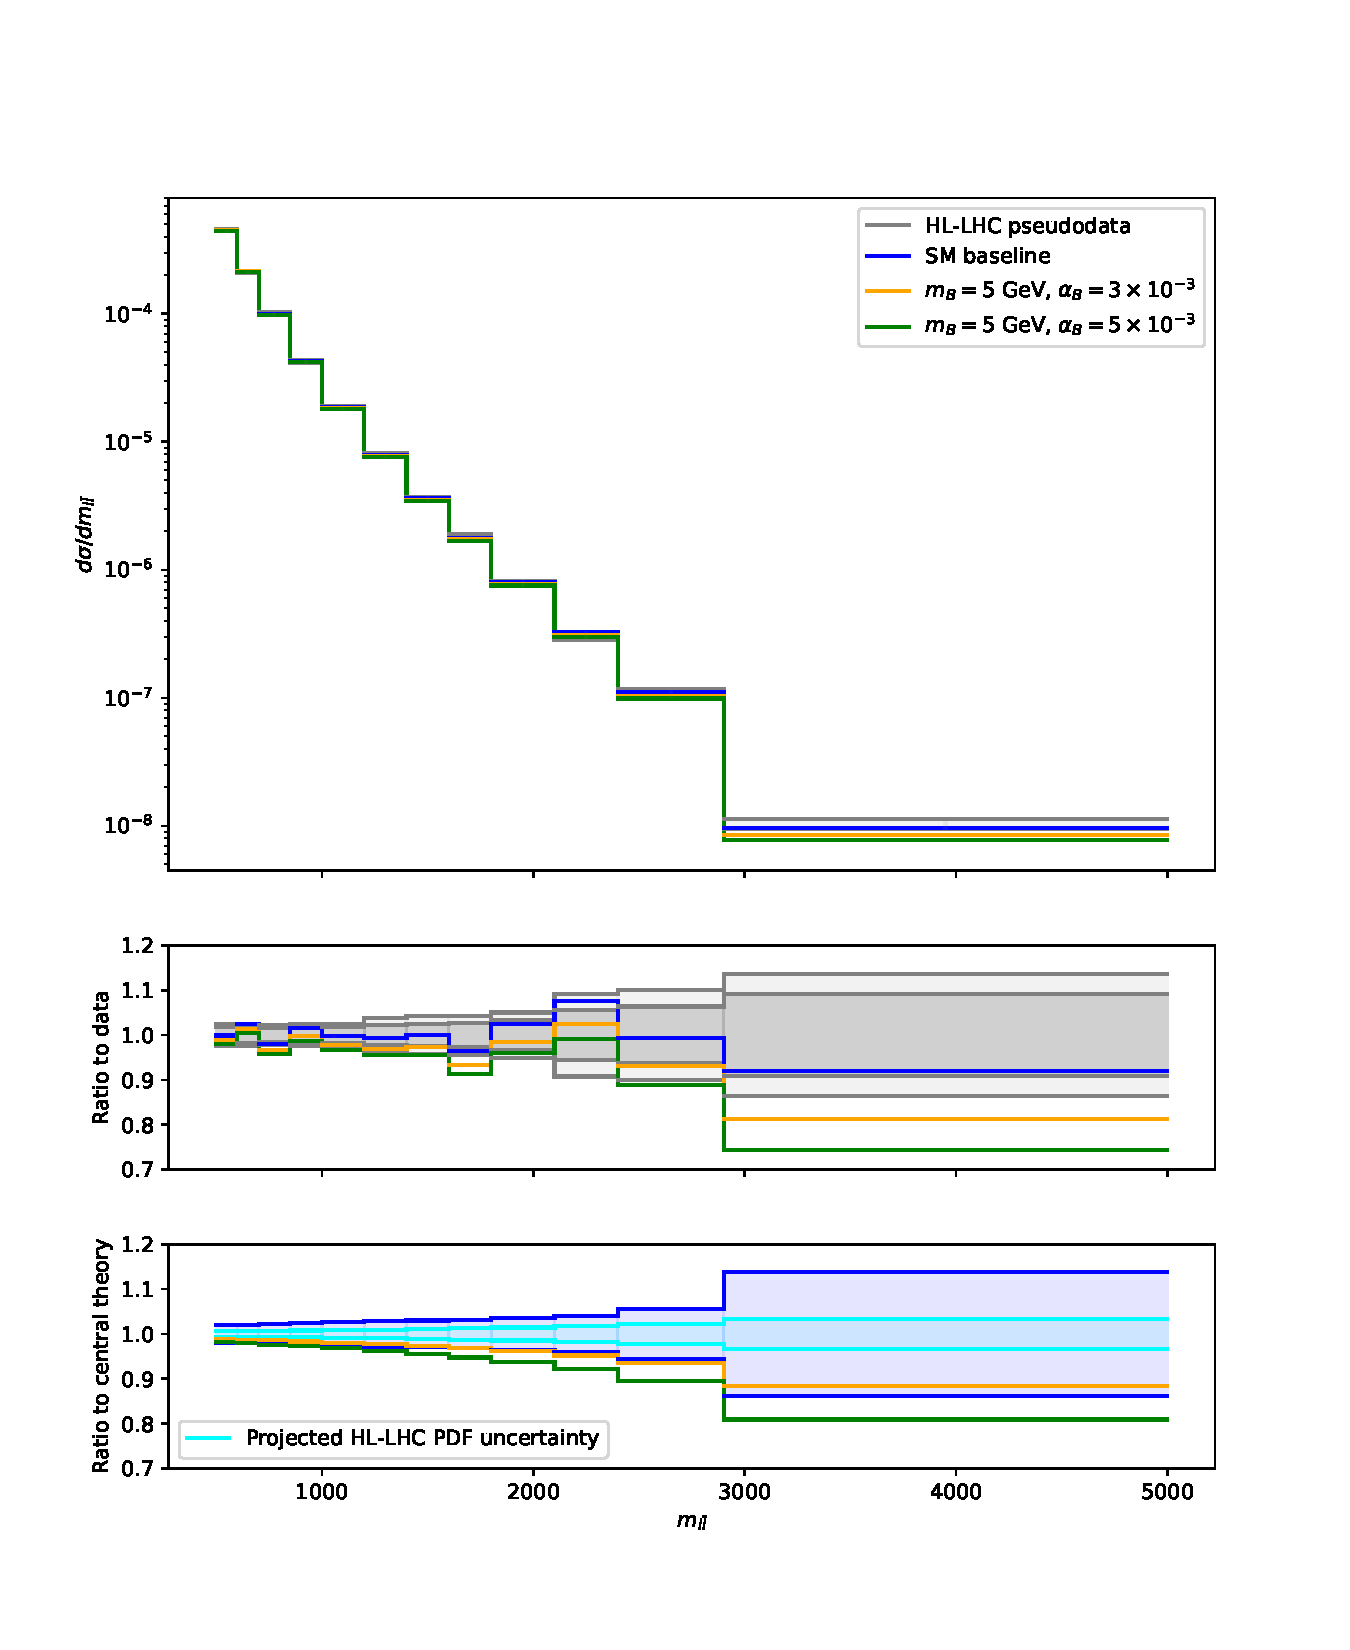
\includegraphics[width=0.9\textwidth]{darkphoton_figures/data_theory_comparison.pdf}
\caption{\textbf{Top:} data-theory comparison between HL-LHC pseudodata in the electron channel generated according to
  Eq.~\eqref{eq:hllhc} (grey, with \textit{optimistic} uncertainties displayed), and the theoretical predictions obtained using
  the NNLO baseline PDF set {\tt NNPDF3.1luxQED} (blue) and
  those obtained using the dark PDF sets produced with parameters $(m_B,\alpha_B) = (5\ \text{GeV},3\times 10^{-3}), (5\ \text{GeV}, 5 \times 10^{-3})$ (yellow, green respectively).
\textbf{Middle:} ratio of the baseline SM central predictions obtained using the baseline, and the central predictions
  obtained using the two representative dark PDF sets, to the central values of the pseudodata.  The relative experimental
  uncertainties in both the {\it optimistic} scenario (dark grey) and
  {\it conservative} scenario (light grey) are displayed. \textbf{Bottom:} ratio of the central predictions obtained using the two
  representative dark PDF sets to the baseline SM central predictions, with both the PDF uncertainty from the baseline PDF set (dark blue) and the projected PDF uncertainty
  at the HL-LHC in the optimistic scenario of ~\cite{Khalek:2018}
  (light blue) displayed.
} 
\label{fig:data-theory}
\end{figure}
%
In Fig.~\ref{fig:data-theory} we display the data-theory comparison
between the HL-LHC pseudodata in the electron channel, generated according to
Eq.~\eqref{eq:hllhc}, and both the SM theoretical predictions obtained using
  the NNLO baseline PDF set {\tt NNPDF3.1luxQED} and the predictions
  obtained using the dark PDF sets produced with the dark photon mass
  and coupling set
  to $(m_B=5\,{\rm GeV},\alpha_B=3\times 10^{-3})$ 
  and $(m_B=5\,{\rm GeV},\alpha_B=5\times 10^{-3})$ respectively. We also display 
 the ratio between the central values of those predictions and the
 central values of the pseudodata as compared to their relative
 experimental uncertainty in both the
 {\it optimistic} and {\it conservative} scenarios.
We see that whilst the SM predictions are within the $1\sigma$
experimental uncertainty (by construction), the dark-photon modified
predictions display significant deviations. 
In the bottom inset we show the ratio between the predictions
obtained in the two representative dark photon scenarios to the
central SM theoretical predictions obtained with the
the baseline SM PDF set. PDF uncertainties are shown; we display
both the current PDF uncertainty of the NNLO baseline PDF set {\tt
  NNPDF3.1luxQED} and the projected PDF uncertainties 
  at the HL-LHC, obtained as described at the beginning of this
  section. Comparing the size of the PDF uncertainties to the size of the
  projected experimental uncertainties at the HL-LHC, we observe
  that whilst the current PDF uncertainties are comparable to the
  experimental uncertainties of the projected data, the projected
  HL-LHC uncertainties are subdominant as compared to the
  experimental uncertainties of the pseudodata.

The $\chi^2$-statistic of the resulting dark PDF set's predictions on high-luminosity high-mass neutral-current DY data is defined as: 
\begin{equation}
\label{eq:chi2stat}
\chi^2(m_B, \alpha_B) := ||\vec{T}(m_B, \alpha_B) - \vec{D}||^2_{\Sigma^{-1}},
\end{equation}
where $||\vec{v}||_{A}^2 = \vec{v}^T A \vec{v}$, $\vec{D}$ is the projected data, 
$\vec{T}(m_B,\alpha_B)$ are the theoretical predictions using a dark
PDF set containing a dark photon of mass $m_B$ and coupling
$\alpha_B$, and $\Sigma$ is the total
covariance matrix (incorporating both experimental and theoretical
uncertainties):
\begin{equation}
\Sigma = \Sigma^{\rm th}+\Sigma^{\rm exp}.
\end{equation}
From Fig.~\ref{fig:data-theory} we observe that, depending on the assumption we make on PDF
uncertainties in the HL-LHC era, it may be important to
include the PDF uncertainties in the theory covariance matrix, while
the component of the theory covariance matrix associated with the
scale uncertainty of the NNLO computation is subdominant. 
Of course, it would be unrealistic to assume that the PDF uncertainty will not decrease as compared to the
  uncertainty of the {\tt NNPDF3.1luxQED} baseline, given that we already know
  that in the updated {\tt NNPDF4.0} set~\cite{NNPDF:2021njg} the uncertainty of the large-$x$
  quarks and antiquarks has already decreased by a sizeable amount
  thanks to the inclusion of precise LHC data. We thus decide to use
  the projected PDF uncertainties determined in~\cite{Khalek:2018}; in particular, we use Scenario 1 of ~\cite{Khalek:2018} (the conservative scenario) when we
  consider the {\it conservative} experimental scenario, and we use Scenario 3 of ~\cite{Khalek:2018} (the most optimistic scenario) when we
  consider the {\it optimistic} experimental scenario.  In Appendix C
  we discuss how our results depend on the assumptions we make on PDF
  uncertainties. 
  Assuming that the projected PDF uncertainties at the HL-LHC that we display in the
  bottom inset of Fig.~\ref{fig:data-theory} are realistic, even in
  the most optimistic scenario they still amount to 4\% to 6\% in the
  largest bins. Therefore, their contribution is much larger than the
  scale uncertainty of the Drell-Yan matrix element at NNLO in
  QCD; hence PDF uncertainty is the dominant theory uncertainty on the
   predictions, and thus it is this contribution that is included in the theory covariance matrix. 

To compute the contribution of PDF uncertainties to the theory
covariance matrix, we build the theoretical covariance as defined in~\cite{Hartland:2019bjb}:
\begin{equation}
\Sigma^{\rm th}_{ij} = \langle d\sigma_i^{{\rm th},(r)} d\sigma_j^{{\rm th},(r)}\rangle_{\rm rep} - \langle d\sigma_i^{{\rm th},(r)}\rangle_{\rm rep} \langle d\sigma_j^{{\rm th},(r)}\rangle_{\rm rep},
\end{equation}
where the theoretical predictions for the differential cross section $d\sigma_i^{{\rm th},(r)}$ are computed using the SM theory and the $r^{\rm th}$
replica from the baseline PDF set, with PDF uncertainties rescaled by
the HL-LHC uncertainty reduction, and averages $\langle \cdot \rangle_{\rm rep}$ are performed over the 
$N_{\rm rep} = 100$ replicas of this PDF set.

We define the difference in $\chi^2$ to be:
\begin{equation}
\Delta \chi^2(m_B, \alpha_B) := \chi^2(m_B, \alpha_B) - \chi^2_0,
\end{equation}
where $\chi^2_0$ is the $\chi^2$-statistic when predictions from the baseline set are used instead. For each fixed $m_B = m_B^*$ in the scan, we then model $\Delta \chi^2(m_B^*,\alpha_B)$ as a quadratic in $\alpha_B$ and determine the point at which $\Delta \chi^2 = 3.8$, corresponding to a confidence of 95\% in a one-parameter scan. Hence, we construct 95\% confidence bounds on $m_B, \alpha_B$ (and hence $m_B, g_B$ via an appropriate conversion) as displayed in~Fig. \ref{fig:limits}. There, the purple (dashed) projected bounds are computed in the conservative scenario excluding (including) the PDF theory covariance matrix, and the green (dashed) projected bounds are computed in the optimistic scenario excluding (including) the PDF theory covariance matrix.

\begin{figure}
\centering
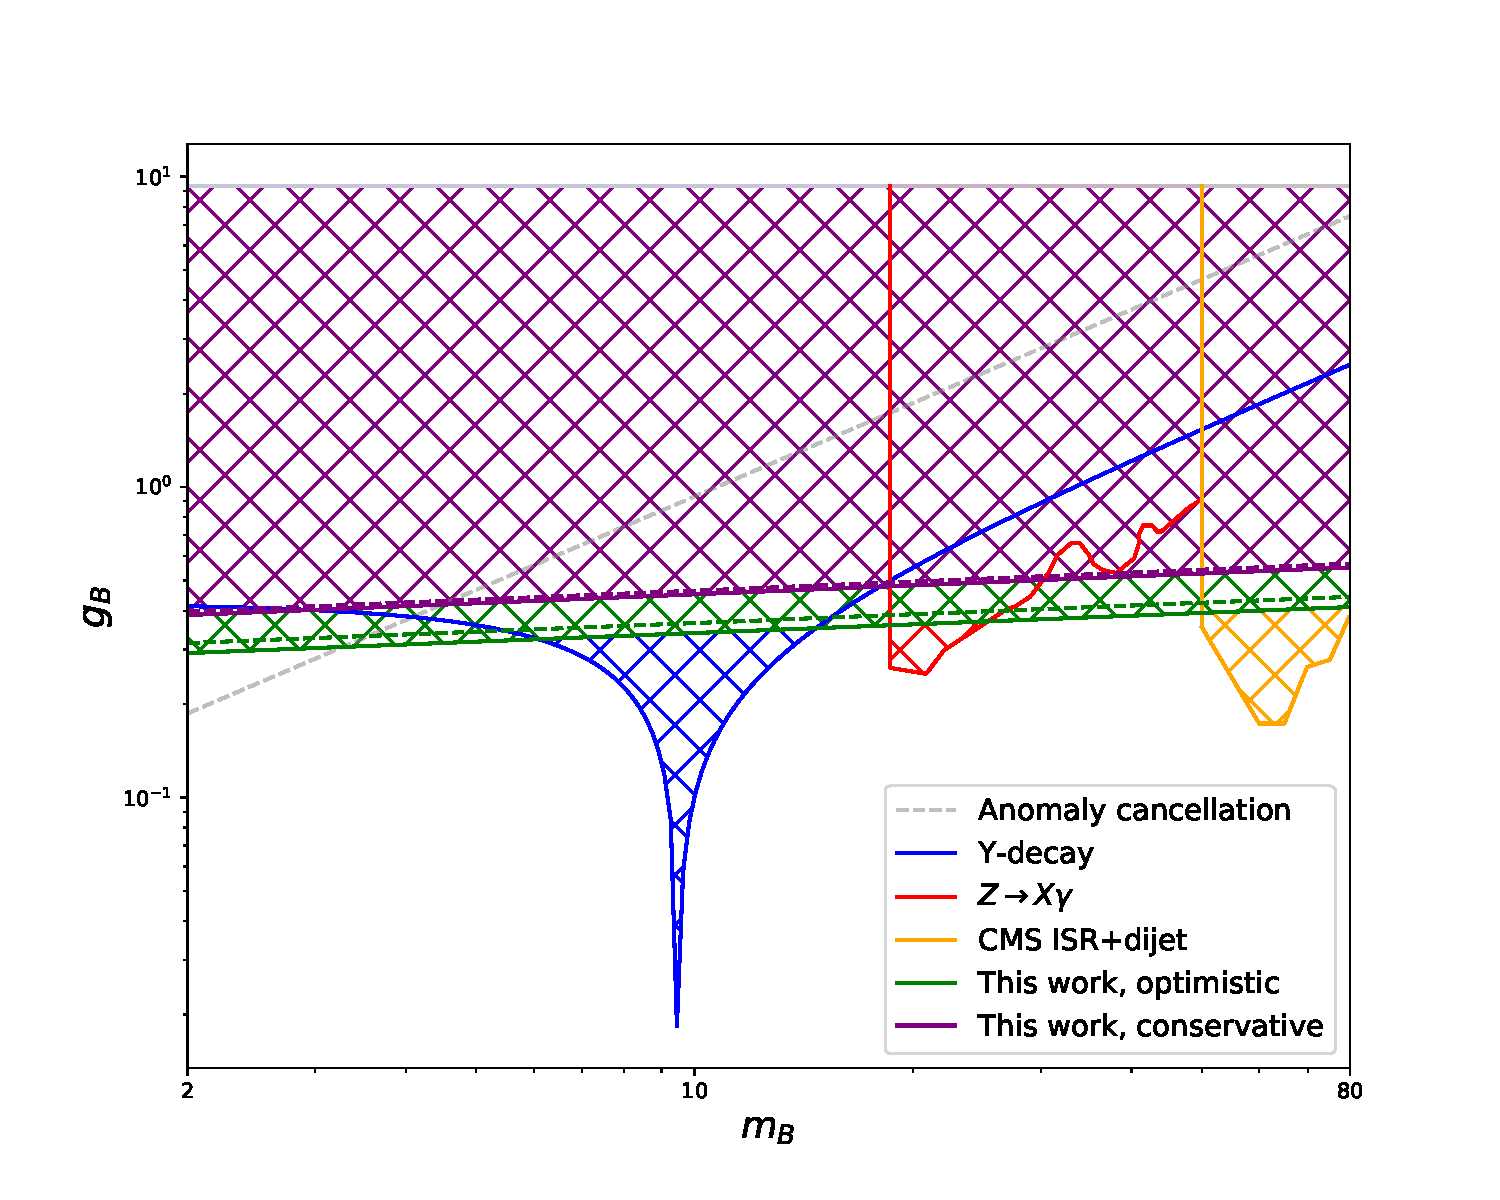
\includegraphics[width=0.95\textwidth]{darkphoton_figures/bounds_plot.pdf}
\caption{Comparison of the projected HL-LHC sensitivity computed in
  this work in the optimistic (green) and conservative (purple) scenarios with the
  existing bounds described in Sec.~\ref{sec:existingconstraints}. The solid green and
  purple lines correspond to projected bounds obtained \textit{excluding} projected PDF uncertainty, whilst the 
  dashed lines correspond to projected bounds obtained \textit{including} projected PDF uncertainty, as discussed in
  the text.}
\label{fig:limits}
\end{figure}

We observe that the projected HL-LHC sensitivity to the detection of a dark photon is competitive with existing experimental bounds, across a large range of possible masses, especially $m_B \in [2,6] \cup [25, 50]\ \text{GeV}$. Even in the most conservative scenario including PDF uncertainty (shown as a dashed purple line), the projected sensitivity remains competitive with experiment. Furthermore, one of the useful features of our projected sensitivity is that it is uniformly excluding across a large range (because of the logarithmic dependence on $m_B$); when compared to individual bounds one at a time, for example the $\Upsilon$-decay bounds, or the anomaly bounds, our projected sensitivity is powerful.



\newpage
\section{Future directions}
\label{sec:dark_future}

There are several approximations made in this chapter which should be lifted in future work, and there are various directions that future studies could pursue based on the method presented here.

First, we note that our projected sensitivity is based on the phenomenological tools that we currently have available; we will be able to make more robust statements with the advent of the HL-LHC. Most importantly new global PDF sets will be made available, which will possibly be accurate to N$^3$LO in QCD, to be used consistently with N$^3$LO computations of the matrix elements. Moreover the associated PDF uncertainty will most certainly include a missing higher order uncertainty component in the PDF uncertainty that is not currently included in any of the global NNLO PDF fits.

Further, the treatment of the dark photon itself could naturally be improved. Here, we make a coarse leading order approximation, based on conjecturing a form for the dark photon PDF and computing the impact of such a PDF on the evolution of the other flavours. Naturally, a more robust analysis would perform a \textit{fit} of a PDF set including dark photon contributions; the expectation would be to treat the dark photon using the \texttt{LUXqed} method in the same manner as the photon. There are some technical barriers to such an analysis, but these could be investigated in future works.

Finally, it would be interesting to ask whether similar analyses could be performed for other BSM particles. A particularly interesting candidate is an \textit{axion}, which depending on the model, might couple to gluons and hence have a significant impact on the evolution of the gluon PDF. This could effect interesting processes like top-pair production, extending works such as the recent Ref.~\cite{Esser:2023fdo}. 


 


\newpage
\chapter{Parton distributions in the SMEFT from high-energy Drell-Yan tails}
\label{chap:smeftdy}

\epigraph{...}{\textit{\\ from ..., \\ by ...}}

\noindent \textit{[This chapter is based on Ref.~\cite{Greljo:2021kvv}, produced in collaboration with Admir Greljo, Shayan Iranipour, Zahari Kassabov, Maeve Madigan, Juan Rojo, Maria Ubiali and Cameron Voisey, and additionally on Ref.~\cite{Madigan:2021uho}, produced in collaboration with Maeve Madigan. My main contributions to the work comprised: the calculation and production of SMEFT $K$-factors for all of the DIS processes entering the study, accurate to next-to-leading order in QCD; benchmarking of the charged current DY $K$-factors against an analytic calculation; running a subset of the fits and analysis, especially in the follow-up study of Ref.~\cite{Madigan:2021uho}, presented in Sect.~\ref{sec:hllhc_extension}.]}\\

\noindent In Chapter~\ref{chap:darkphoton}, we focussed on simultaneous extraction of PDFs and BSM parameters in the case of a dark photon model, where the only BSM particle was \textit{light}. Whilst this model was motivated by the desire to provide a possible dark matter candidate, it is only one of plethora of models which we could have investigated. This suggests the need for a more general framework in which to search for BSM physics.

In the case of \textit{heavy} New Physics, this can be facilitated through the language of \textit{effective field theories} (EFTs). In this chapter, we shall introduce the idea of treating the Standard Model within the effective field theory approach. We shall subsequently present a study wherein we simultaneously extract PDFs and two couplings drawn from the Standard Model EFT, using both DIS and DY data; we shall find that the interplay between PDFs and the Standard Model EFT is mild with the current data, but when we move to using projected HL-LHC data (just as in Sect.~\ref{subsec:dark_constraints}), the interplay becomes significant. This study motivates a more comprehensive extraction of PDFs alongside Standard Model EFT couplings in the top sector, which we present in Chapter~\ref{chap:top}. Further, we present a first glimpse of extraction of PDFs from projected data \textit{which contains New Physics} in Sect.~\ref{sec:hllhc_extension}, an idea which will be investigated in much greater detail in Chapter~\ref{chap:contamination}.

\section{Effective field theories and the SMEFT}
\label{sec:eft_intro}
The language of \textit{effective field theory} (EFT) provides a twofold advantage when discussing QFTs: the method of \textit{top-down} EFT can simplify calculations by removing degrees of freedom from a theory which are not relevant at low energy scales, whilst the method of \textit{bottom-up} EFT allows us to parametrise deviations from a good low-energy theory due to unknown high-energy physics. 

In this section, shall provide a brief review of both of these techniques, especially bottom-up EFT as applied to the SM. We begin in Sect.~\ref{subsec:eft_background} with a basic demonstration of the key ideas involved in EFT, using a toy model that comprises a single light fermion and a single heavy scalar. In Sect.~\ref{subsec:the_smeft}, we then apply these ideas to the SM, describing how it can be treated in the bottom-up EFT approach resulting in an effective field theory called the \textit{Standard Model Effective Field Theory} (SMEFT). The remainder of the chapter is dedicated to fitting PDFs and two parameters drawn from the SMEFT.

\subsection{Introduction to effective field theories}
\label{subsec:eft_background}

To introduce the concept of an \textit{effective} theory, we follow the example of Sect. 4.1 of Ref.~\cite{Petrov:2016azi}, and consider a field theory comprising a single real scalar field $\phi$ and a single fermionic field $\psi$, with squared masses $M^2, m^2$ respectively, and with Lagrangian density:
\begin{equation}
\label{eq:yukawa}
\mathcal{L} = \frac{1}{2} (\partial \phi)^2 - \frac{1}{2} M^2 \phi^2 + \overline{\psi}(i \slashed{\partial} - m) \psi - g \phi \overline{\psi} \psi.
\end{equation}
Suppose additionally that $\phi$ is much heavier than $\psi$, with $M^2 \gg m^2$, so that $\phi$ cannot be produced on-shell in any current experiments, say. The partition function for the theory takes the form:
\begin{equation}
\label{eq:partition_function}
\mathcal{Z} = \int \mathcal{D}\phi \mathcal{D}\psi \exp\left(i \int d^4x \left( \frac{1}{2} (\partial \phi)^2 - \frac{1}{2} M^2 \phi^2 + \overline{\psi}(i \slashed{\partial} - m) \psi - g \phi \overline{\psi} \psi\right) \right),
\end{equation}
where $\mathcal{D}\phi, \mathcal{D}\psi$ indicate the measures over the relevant functional spaces.\footnote{Which of course, in the strictest sense, do not actually exist in a strict mathematical sense.} By performing the integral over $\phi$, we can derive an equivalent theory entirely in terms of $\psi$; this theory will apply below the scale at which $\phi$ can be produced on-shell. 

To perform the integral, it is convenient to change variables, introducing:
\begin{equation}
\phi'(x) := \phi(x) + ig \int d^4y\ D_F(x-y)\overline{\psi}(y) \psi(y),
\end{equation}
where $D_F$ is the free-space propagator for the $\phi$-field, given by:
\begin{equation}
\label{eq:propagator}
D_F(z) := \int \frac{d^4k}{(2\pi)^4} \frac{i}{k^2 - M^2 + i\epsilon} e^{-ik \cdot z}.
\end{equation}
Making this change of variables in Eq.~\eqref{eq:partition_function}, we obtain:
\begin{align}
\mathcal{Z} &= \int \mathcal{D}\phi' \mathcal{D}\psi \exp\left(i \int d^4x\ \overline{\psi}(i \slashed{\partial} - m) \psi \right) \exp\left( i \int d^4x \left( \frac{1}{2} (\partial \phi')^2 - \frac{1}{2}M^2 {\phi'}^2\right) \right) \notag \\[1.5ex]
&\qquad \cdot \exp\left( i \int d^4x d^4y\ ig^2\overline{\psi}(x) \psi(x)D_F(x-y)\overline{\psi}(y) \psi(y) \right).
\end{align}
The integral over $\phi'$ can now be performed, producing an irrelevant overall constant of normalisation. The resulting theory then has the non-local Lagrangian:
\begin{equation}
\label{eq:first_try_eft}
\mathcal{L}_{\text{eff}} = \overline{\psi}(i \slashed{\partial} - m) + ig^2 \int d^4y\ \overline{\psi}(x) \psi(x) D_F(x-y) \overline{\psi}(y)\psi(y).
\end{equation}
In the limit $M^2 \rightarrow \infty$, we may expand the denominator of $D_F$ in Eq.~\eqref{eq:propagator} in powers of $k^2/M^2$, which to a leading approximation gives:
\begin{equation}
D_F(z) = - \frac{i}{M^2} \delta^4(z),
\end{equation}
hence we may rewrite the Lagrangian Eq.~\eqref{eq:first_try_eft} as:
\begin{equation}
\label{eq:top_down_eft}
\mathcal{L}_{\text{eff}} = \overline{\psi}(i \slashed{\partial} - m)\psi + \frac{g^2}{M^2} (\overline{\psi}\psi)^2 + O\left( \frac{1}{M^4} \right). 
\end{equation}
We say that this theory is an \textit{effective theory}, valid below the energy scale $M$, with \textit{ultraviolet (UV) completion} given by the original theory. Important features to note are the following:
\begin{enumerate}[label = (\roman*)]
\item Integrating out the field $\phi$ has resulted in a Lagrangian containing a \textit{non-renormalisable} term, $(\overline{\psi}\psi)^2$; this can be seen by counting mass dimensions, which in this case shows that this operator is in fact a dimension \textit{six} operator. In a QFT that we expect to hold to arbitrarily high energy scales, such terms are not permissible. However, in our \textit{effective} theory, there is no such stringent requirement; we indeed expect the theory to break down at the scale $M$, and so non-renormalisable terms are in fact allowed.

\item The non-renormalisable operators in the effective theory have been organised into a series, with their associated couplings suppressed by increasing powers of $1/M^2$. By counting mass dimensions, we see that the higher the dimension of the operator, the more subleading its effect. 
\end{enumerate}

\paragraph{Top-down vs bottom-up.} The construction above is known as \textit{top-down} construction of an EFT. In this paradigm, we begin with a UV-complete theory, and then we integrate out modes to produce an effective theory containing non-renormalisable operators; the theory is then valid only up to some large energy scale. Top-down construction of an EFT is particularly useful if we wish to simplify calculations by ignoring degrees of freedom which are not relevant at the energy scale of study (for example, the $W$ and $Z$ bosons are often integrated out of the electroweak theory when performing low-energy calculations, resulting in the \textit{Fermi effective theory}).

On the other hand, the EFT approach can also be applied in a \textit{bottom-up} fashion. Suppose that we have a renormalisable theory which works well at low energies, but we expect to break down at some higher energy scale, making way for another theory which contains additional, unknown, heavy degrees of freedom. The low-energy limit of this high-energy theory must match our low-energy theory; in particular, our low-energy theory should be considered the leading approximation in a top-down EFT approach to the unknown high-energy theory. Therefore, we can build more precise approximations to the high-energy theory by adding on all non-renormalisable operators to the low-energy Lagrangian, built from the low-energy degrees of freedom and respecting any symmetries of the low-energy theory that we believe still hold in the high-energy theory. These non-renormalisable operators can be organised in terms of importance by their \textit{mass dimension}, since dimensional analysis tells us their couplings must be increasingly suppressed by a characteristic scale of the high-energy physics (e.g. the mass of the lowest-energy degree of freedom that is integrated out at low energies) as the mass dimension of the operator increases.

For a concrete example, suppose that we believe that at low energies, Nature is described by the fermionic Lagrangian:
\begin{equation}
\mathcal{L}_{\text{low}} = \overline{\psi} (i \slashed{\partial} - m) \psi.
\end{equation}
This theory has a $U(1)$ global vector symmetry $\psi \mapsto e^{i\theta}\psi$ and a $U(1)$ global axial symmetry $\psi \mapsto e^{i\theta \gamma^5} \psi$, which perhaps we believe to be fundamental (and suppose we also believe that Lorentz symmetry is fundamental). We can describe theories which have the low-energy limit $\mathcal{L}_{\text{low}}$ by adding on all possible higher-dimensional operators which respect the symmetry, organised by their mass dimension, to produce a \textit{bottom-up} EFT which is the low-energy limit of the unknown high-energy theory. Such operators can only be built from $\psi, \overline{\psi}$ and the derivative $\partial$; the mass dimensions of these objects are $[\psi] = [\overline{\psi}] = 3/2$ and $[\partial] = 1$, respectively. Considering the ways in which these objects can be combined at each mass dimension, we therefore obtain an EFT approximation of the form (up to operators of mass dimension $6$):
\begin{equation}
\label{eq:first_try_bottom_up_eft}
\mathcal{L}_{\text{low}}^{\text{EFT}} = \overline{\psi}(i\slashed{\partial} - m) \psi - \frac{g_5}{\Lambda} \overline{\psi} \partial^2 \psi -  \frac{g_6^{(1)}}{\Lambda^2} (\overline{\psi}\psi)^2 - \frac{g_6^{(2)}}{\Lambda^2} \overline{\psi} \partial^2 \slashed{\partial} \psi - ...,
\end{equation}
where $\Lambda$ is some characteristic scale of New Physics.

Importantly, some of these operators can be removed by considering the \textit{equations of motion} of the theory (a point we shall shortly return to when we discuss EFT bases below). The fermion $\psi$ obeys the free Dirac equation in the low-energy theory, given by:
\begin{equation}
(i \slashed{\partial} - m)\psi = 0,
\end{equation}
which yields the Klein-Gordon equation $(\partial^2 + m^2)\psi = 0$ when the operator $(i\slashed{\partial} - m)$ is applied a second time. Therefore, whenever a second derivative term appears, we may replace $\partial^2$ with $-m^2$. As a result, the effective theory can be simplified to:
\begin{equation}
\label{eq:bottom_up_eft}
\mathcal{L}_{\text{low}}^{\text{EFT}} = \overline{\psi}(i\slashed{\partial} - m) \psi -  \frac{g_6}{\Lambda^2} (\overline{\psi}\psi)^2 - ...\ .
\end{equation}
The reason that we can apply the \textit{free} equations of motion here, even though we believe the fermion is actually coupled in the high-energy theory, is that the corrections to the free equations of motion enter at order $1/\Lambda$, so are suppressed when inserted into the Lagrangian and can be neglected at the order we are considering. The unknown coefficients in the expansion, $g_6$, etc, are called \textit{Wilson coefficients}.

As expected, if we know that the UV-completion of the theory is given by Eq.~\eqref{eq:yukawa}, the bottom-up EFT Eq.~\eqref{eq:bottom_up_eft} can be \textit{matched} to the UV-complete theory. In this case, this can be achieved by comparing Eq.~\eqref{eq:top_down_eft} with Eq.~\eqref{eq:bottom_up_eft}, where we identify:
\begin{equation}
\frac{g_6}{\Lambda^2} = -\frac{g^2}{M^2}.
\end{equation}
In more complicated scenarios, matching can be performed order-by-order in perturbation theory by computing processes using both the diagrams of the UV-complete theory and the diagrams of the effective theory, and then comparing the results. There are also other methods of matching available, including \textit{functional matching} (see for example Ref.~\cite{Henning:2014wua}). 

\paragraph{Renormalisability.} By their very construction, effective theories contain non-renormalisable operators, and hence are not renormalisable theories. However, as we mentioned above, this is no problem in the EFT philosophy, since we do not expect EFTs to hold to arbitrarily high energies. 

Further, whilst EFTs are not renormalisable \textit{per se}, they do have the useful property that they are renormalisable \textit{order by order} in $1/\Lambda$, where $\Lambda$ is the characteristic scale of the New Physics. This manifests in the following way: if we perform a loop calculation in our EFT, we shall find that we obtain divergent contributions which can only be cancelled by counterterms with higher mass dimensions than those considered at a fixed order in $1/\Lambda$. However, the divergent contribution will itself be multiplied by a higher power in $1/\Lambda$ than the fixed order we are considering; hence, it can be dropped. Details of such a calculation are presented in Sect. 5.4 of Ref.~\cite{Manohar:2018aog}.

Renormalisation of an EFT also results in \textit{running} of the Wilson coefficients in the EFT. We will neglect this effect in the rest of the thesis, since it will be subleading in all scenarios considered, but it is worth noting that the coefficients are not constants.

\paragraph{EFT bases.} In the case of a more general bottom-up EFT, with many more low-energy degrees of freedom, there will be a vast array of possible operators that can be written down at a given mass dimension in the EFT expansion. Crucially, these operators \textit{may not be independent}. Generically, there are two ways in which operators may be dependent on one another:
\begin{enumerate}[label = (\roman*)]
\item \textbf{Equations of motion.} The operators might be related by the \textit{equations of motion} of the low-energy theory. We already saw an example of this when reducing Eq.~\eqref{eq:first_try_bottom_up_eft} to Eq.~\eqref{eq:bottom_up_eft}.
\item \textbf{Integration by parts.} The operators might be related by \textit{integration by parts}. Consider, for example, the following pair of operators:
\begin{equation}
\phi^2 \partial^2 \phi, \qquad \qquad \phi (\partial\phi)^2,
\end{equation}
built from a scalar field $\phi$ and the derivative $\partial_{\mu}$. On the surface, these appear to be separate operators. However, they are in fact the same operator, when related by integration by parts:
\begin{equation}
\int d^4x\ \phi^2 \partial^2 \phi = -\int d^4x\ \partial(\phi^2) \cdot \partial \phi = -2 \int d^4x\ \phi (\partial \phi)^2,
\end{equation}
assuming that boundary terms decay at infinity. Therefore, if we were to na\"{i}vely insert the sum $g \phi^2 \partial^2 \phi + g' \phi (\partial \phi)^2$, we would find that it in all processes the Wilson coefficients $g, g'$ would enter in the combination $g' - 2g$; we would never be able to determine them independently of one another.
\end{enumerate}
It follows that in any construction of a bottom-up EFT, to avoid redundancy we should endeavour to find a minimal set of operators (at each mass dimension) which are independent of one another, so that their associated Wilson coefficients can additionally be determined independently of one another. Such a minimal set is called a \textit{basis} for the EFT at the given mass dimension; this notion will be immediately useful when we construct the SMEFT using the so-called \textit{Warsaw basis} in the following section, Sect.~\ref{subsec:the_smeft}.

\subsection{The SMEFT}
\label{subsec:the_smeft}
The framework of bottom-up EFTs can naturally be applied to the Standard Model itself, producing an EFT known as the \textit{Standard Model Effective Field Theory} (SMEFT) (see e.g. Ref.~\cite{Brivio:2017vri} for a review). 
%\cite{Weinberg:1979sa,Buchmuller:1985jz,Georgi:1994qn,Giudice:2007fh,Grzadkowski:2010es,Alonso:2013hga,Jenkins:2013wua,Jenkins:2013zja,Henning:2014wua,Brivio:2017vri,Wells:2015uba,Englert:2019zmt,Fuentes-Martin:2020udw,Cohen:2020qvb}. 
Following the procedure outlined above, the Lagrangian of the SMEFT must take the form:
\begin{equation}
\mathcal{L}_{\text{SMEFT}} = \mathcal{L}_{\text{SM}} + \sum_{d=5}^{\infty} \sum_{i=1}^{n_d} \frac{c_d^{(i)}}{\Lambda^{d-4}} \mathcal{O}_{d}^{(i)},
\end{equation}
where $\mathcal{L}_{\text{SM}}$ denotes the Lagrangian of the Standard Model, and $\mathcal{O}_{d}^{(i)}$ denotes the $i$th operator in a basis for the $d$-dimensional operators built from the SM fields and obeying the SM symmetries (Lorentz symmetry and gauge symmetry). Here, $n_d$ denotes the number of independent operators of mass dimension $d$, $c_d^{(i)}$ denotes the $i$th Wilson coefficient at mass dimension $d$, and $\Lambda$ represents a characteristic scale of New Physics.

The types of operators that arise at dimension $d=5$, $d=6$ in the expansion have been completely classified. The operators at dimension $d=5$ are known as \textit{Weinberg operators}, and are all lepton number violating; strong constraints on their respective Wilson coefficients from LEP mean that these operators are usually ignored. At dimension $d=6$, there are a total of $n_6 = 2499$ independent operators, parametrised by the so-called \textit{Warsaw basis}, introduced in Ref.~\cite{Grzadkowski:2010es}. It is the dimension six terms which we shall be most interested in throughout this thesis. The complete list of operators in the Warsaw basis is presented in Ref.~\cite{Grzadkowski:2010es} in Tables 2 and 3; we shall only require a small subset of these operators in the sequel.
 

\section{Parton distributions in the SMEFT}
\label{sec:introduction}
Accurate measurement of observables at high energies offers one of the most promising avenues towards an indirect discovery of BSM physics at the LHC. While the collider has now (almost) reached the design energy, its integrated luminosity continues to grow
steadily, thus greatly facilitating dedicated studies of the
(currently statistics-limited) high-energy tails of distributions. Furthermore, many higher-dimensional SMEFT operators in the Warsaw basis introduced in Sect.~\ref{subsec:the_smeft} induce deviations from the SM which grow
with the energy of the partonic collision, enhancing the BSM sensitivity
of these high-energy tails.
%
For instance, in the Drell-Yan process,  the na\"{\i}ve  scaling of the $\psi \psi \to \psi \psi$ scattering
amplitude in an underlying EFT description leads to an amplitude
$\mathcal{A} \propto E^2 / \Lambda^2$,  where $E$ is the energy of the process and $\Lambda$ is the New Physics scale.
%
Thus, rather generically, a less precise measurement of a high-mass tail can compete with a low-energy precision measurement due to this energy enhancement, which can be traced back to the preservation of unitarity.
%
This property leads to the somewhat unintuitive result that
the study of the high-energy lepton tails in the Drell-Yan process represents a competitive probe
of BSM dynamics compared to electroweak precision tests and low-energy
flavour physics test.
%a remarkable fact that has attracted a lot of attention recently.

However, in order for the SMEFT interpretation of these high-energy tails
to convincingly uncover a BSM effect, it becomes crucial to ensure
full control over the SM inputs and their
uncertainties, such as those associated to the PDFs~\cite{Gao:2017yyd};
as described in Sect.~\ref{sec:globalfits}, this requires us checking that
eventual BSM deviations arising in high-energy tails are not being
inadvertedly reabsorbed into the PDFs, entailing the need for a simultaneous
extraction of PDFs and SMEFT couplings.

A first take on this challenge was presented in a proof-of-concept study~\cite{Carrazza:2019sec} where
the simultaneous determination of PDFs and SMEFT coefficients from deep inelastic scattering (DIS)
structure functions was demonstrated.
%
There, it was found that the SMEFT corrections can indeed be partially reabsorbed into the PDFs
but also that it is possible to robustly disentangle
QCD and BSM effects by exploiting their different energy scaling.

The main goal of the rest of this chapter is to extend this approach to LHC processes, specifically with the
joint determination of PDFs and EFT coefficients from DIS and Drell-Yan data.
%
Drell-Yan processes in general, and high-mass measurements in particular,
provide information on the light quark and anti-quark PDFs in a broad region of $x$ representing
an important ingredient in modern global PDF fits~\cite{Ball:2014uwa,Ball:2017nwa,Hou:2019efy,Bailey:2020ooq}.
%
Furthermore, high-mass Drell-Yan data will be instrumental at the High-Luminosity LHC (HL-LHC)
to pin down the large-$x$ PDFs~\cite{Khalek:2018mdn}.
%
Considering that SMEFT signals can lead to significant deviations from the SM
in these same high-energy DY tails, one would like to assess to what extent they
can be reabsorbed into the PDFs and to define strategies to
separate QCD from BSM effects.

In order to interpret the Drell-Yan data in the SMEFT framework in this chapter,
we formulate a simple, yet motivated, benchmark scenario~\cite{Farina:2016rws};
in particular, we consider the $\hat{W}$ and $\hat{Y}$ electroweak parameters generated in 
universal theories that modify the electroweak gauge boson propagators 
and lead to flavour-universal deviations which grow with the invariant mass. This scenario is discussed
in detail in Sect.~\ref{sec:dy_scenarios}. Subsequently, in Sect.~\ref{sec:dy_data} we summarise the datasets (taken to be
exclusively DIS and DY sets to ensure a theoretically consistent description of the PDFs
in the SMEFT) used in the 
analysis, and the corresponding theoretical calculations. In Sect.~\ref{sec:res1} we present the 
results for the simultaneous determination of the
SMEFT coefficients and the PDFs from the available high-mass DY data
from LHC Run I and Run II, in the two
scenarios presented in Sect.~\ref{sec:dy_scenarios} and assess how they
modify the interpretation of BSM searches based on the SM PDFs.
%
In Sect.~\ref{sec:hllhc} we present a summary of the constraints we find on the two
scenarios we consider and we assess the outcome of a joint
PDF and SMEFT analysis using projections for the HL-LHC, just as we did
in Sect.~\ref{sec:dark_pheno}.
% 
Finally, in Sect.~\ref{sec:hllhc_extension}, we present the results of a follow-up study
where we consider the outcome of a joint PDF and SMEFT analysis using projections for
the HL-LHC which have had New Physics injected into the tails; that is, we ask how our 
analysis changes \textit{if} New Physics is present during the HL phase of the LHC.

\section{The SMEFT scenario: oblique corrections}
\label{sec:dy_scenarios}

In this section we present the SMEFT benchmark scenario that will be
used in this chapter to interpret the LHC Drell-Yan processes. This 
scenario belongs to the class of electroweak precision tests and is
sensitive to a broad range of UV-complete theories proposed in the literature.

The \textit{oblique corrections}, as originally proposed in~\cite{Peskin:1991sw,Altarelli:1991fk}, play a key role in testing theories beyond the Standard Model. They parametrise the self-energy $\Pi_V(q^2)$ of the electroweak gauge bosons $W^a_\mu$ and $B_\mu$,  where $V = W^3 W^3$, $B B$, $W^3 B$, and $W^+ W^-$.
%
Truncating the momentum expansion at order $q^4$, while imposing proper normalisation and symmetry constraints, one concludes that there are only four oblique
parameters which can be identified with dimension-six operators in the SMEFT.
%
These are the well-known  $\hat{S}$, $\hat{T}$, $\hat{W}$, and $\hat{Y}$
parameters~\cite{Barbieri:2004qk}.
%
The parameters $\hat{S}$ and $\hat{T}$ are well constrained from precision
LEP measurements~\cite{Barbieri:2004qk} and grow slowly with $q^2$,
while $\hat{W}$ and $\hat{Y}$ scale faster implying that their effects will be
enhanced for the high-energy dilepton tails at the LHC~\cite{Farina:2016rws}; 
while $\hat{T} = {\mathcal O}(q^0)$ and $\hat{S} = {\mathcal O}(q^2)$ ,
instead one has that $\hat{W},\hat{Y} = {\mathcal O}(q^4)$.
%
%In the universal basis (see e.g.~\cite{Englert:2019zmt}), the $\hat{W}$ and $\hat{Y}$
%parameters are the Wilson coefficients associated to the following two operators:
%\begin{equation}
%\label{eq:WY}
%\mathcal{L}_{\rm SMEFT} \supset -\frac{\hat{W}}{4 m_W^2} (D_\rho W^a_{\mu\nu})^2 -\frac{\hat{Y}}{4 m_W^2} (\partial_\rho B_{\mu\nu})^2 ~,
%\end{equation}
%%
%where $m_W$ indicates the $W$-boson mass, and $D_\rho$ is the covariant derivative.
%
%The physical effects of the operators in Eq.~(\ref{eq:WY}) on the Drell-Yan process
%arise from the difference in the propagators through the self-energy modifications, see Eq.~(1) of Ref.~\cite{Farina:2016rws}.

Whilst these operators can be written initially as parametrising self-energies of the 
electroweak bosons,\footnote{See e.g. Ref.~\cite{Englert:2019zmt} where they are written in terms of the \textit{universal basis} for the SMEFT, where they are defined by:
\begin{equation*}
\label{eq:WY}
\mathcal{L}_{\rm SMEFT} \supset -\frac{\hat{W}}{4 m_W^2} (D_\rho W^a_{\mu\nu})^2 -\frac{\hat{Y}}{4 m_W^2} (\partial_\rho B_{\mu\nu})^2.
\end{equation*}
} using the equation of motions they can be rotated to be written in terms of the following four-fermion operators:
\begin{equation} \label{eq:JJ}
\mathcal{L}_{\rm SMEFT} \supset -\frac{g^2 \hat{W}}{2 m_W^2} \, J^{a}_{L \mu} J^{a \mu}_L -\frac{ g_Y^2 \hat{Y} }{2 m_W^2} \, J_{Y \mu} J^\mu_Y ~~,
\end{equation}
where $J_L$ and $J_Y$ are $SU(2)_L$ and $U(1)_Y$ conserved fermionic currents,
\begin{equation}
J^{a \mu}_L =  \frac{1}{2} \sum_{f = q, l}  \bar f \sigma^a \gamma^\mu f ~~,\quad ~~ J^\mu_Y= \sum_{f = q, l, u, d, e}  Y_f\,\bar f \gamma^\mu f~~.
\end{equation}
Here $q$, $l$ are the SM quark and lepton left-handed doublets, while $u$, $d$, $e$ are 
the right-handed singlets. Also, $g$ and $g_Y$ are the corresponding electroweak gauge couplings,
$\sigma^a$ are the Pauli matrices, and the hypercharges are given by $Y_f = 1/6$, $-1/2$, $2/3$, $-1/3$, and $-1$ for $q,l,u,d,e$, respectively. Summation over flavour indices is assumed, which implies
that in this scenario the fermionic currents respect the $U(3)^5$
global flavour symmetry.

Expanding Eq.~\eqref{eq:JJ}, one can relate the $\hat{W}$ and $\hat{Y}$ parameters
to the coefficients of dimension-six operators in the Warsaw basis introduced in Sect.~\ref{subsec:the_smeft}.
%
There, the operators  relevant to the description of the Drell-Yan process are given by:
\begin{equation}
\begin{aligned}\label{eq:Warsaw}
\mathcal{O}_{ld} &= (\bar  l\gamma_\mu l)(\bar d \gamma^\mu d) \,, 
&
\mathcal{O}_{lu} &= (\bar  l\gamma_\mu l)(\bar u \gamma^\mu u) \,,
&
\mathcal{O}_{lq}^{(1)} &= (\bar l \gamma^\mu l) (\bar  q\gamma_\mu q)\,,   
\\
\mathcal{O}_{ed} &= (\bar  e\gamma_\mu e)(\bar d \gamma^\mu d) \,, 
&
\mathcal{O}_{eu} &= (\bar  e\gamma_\mu e)(\bar u \gamma^\mu u) \,,
&
\mathcal{O}_{qe} &=  (\bar  q\gamma_\mu q) (\bar e \gamma^\mu e)\,,
\\
\mathcal{O}_{lq}^{(3)} &=(\bar l \sigma^a \gamma^\mu l)  (\bar  q \sigma^a \gamma_\mu q) \, .
\end{aligned}
\end{equation}
Note the flavour indices are contracted within the brackets, for example $\bar  l\gamma_\mu l \equiv \bar  l^1 \gamma_\mu l^1 + \bar  l^2 \gamma_\mu l^2 + \bar  l^3 \gamma_\mu l^3$. 
%
Taking into account this matching between the $\hat{W}$ and $\hat{Y}$ parameters
and the corresponding Wilson coefficients
in the Warsaw basis,
we can express the SMEFT Lagrangian in this scenario, Eq.~(\ref{eq:JJ}), as follows:
\begin{align}\label{eq:WYWarsaw}
\mathcal{L}_{\rm SMEFT}=\mathcal{L}_{\rm SM}   &-\frac{g^2 \hat{W}}{4
                                                 m_W^2}
                                                 \mathcal{O}_{lq}^{(3)}
                                                 - \frac{ g_Y^2
                                                 \hat{Y} }{m_W^2}
                                                 \Big(Y_l Y_d \,
                                                 \mathcal{O}_{ld} +
                                                 Y_l Y_u \,
                                                 \mathcal{O}_{lu}
                                                 \nonumber \\&+Y_l Y_q
  \, \mathcal{O}_{lq}^{(1)} + Y_e Y_d \, \mathcal{O}_{ed} + Y_e Y_u \,
  \mathcal{O}_{eu} + Y_e Y_q \, \mathcal{O}_{q e} \Big) \,.
\end{align}
The parametrisation in Eq.~(\ref{eq:Warsaw}) was implemented using the {\tt SMEFTsim} package~\cite{Brivio:2017btx} and cross-checked against the reweighting method used in Ref.~\cite{Greljo:2017vvb} (see also~\cite{Ricci:2020xre}).

The analysis in Ref.~\cite{Farina:2016rws} reports the following 95\% confidence level intervals on $\hat{W}$ assuming $\hat{Y}=0$,
\begin{equation}
\begin{split}
\hat W &\in \left[ - 3, 15 \right]\times 10^{-4}~\textrm{(ATLAS 8 TeV, 20.3 fb$^{-1}$~\cite{Aad:2016zzw})}~,\\
\hat W &\in \left[ - 5, 22 \right]\times 10^{-4}~\textrm{(CMS 8 TeV, 19.7 fb$^{-1}$~\cite{CMS:2014jea})}~,
\end{split}
\end{equation} 
as well as, the 95\% confidence level intervals for $\hat{Y}$ assuming $\hat{W}=0$,
\begin{equation}
\begin{split}
\hat Y &\in \left[ - 4, 24 \right]\times 10^{-4}~\textrm{(ATLAS 8 TeV, 20.3 fb$^{-1}$~\cite{Aad:2016zzw})}~,\\
\hat Y &\in \left[ - 7, 41 \right]\times 10^{-4}~\textrm{(CMS 8 TeV, 19.7 fb$^{-1}$~\cite{CMS:2014jea})}~.
\end{split}
\end{equation}
These bounds have been computed assuming SM PDFs. In the rest of this chapter,
for this benchmark scenario, we see how the limits based on SM PDFs
are modified once a consistent determination of the SMEFT PDFs is
performed, requiring a simultaneous fit of the PDFs together with the
$\hat{W}$ and $\hat{Y}$ parameters from the high-mass Drell-Yan distributions. 


\section{Data, theory, and fit settings}
\label{sec:dy_data}

In Sect.~\ref{sec:dy_dataset} we present the LHC experimental data  that will be used in this chapter
for the simultaneous determination of the PDFs and
the EFT coefficients from high-mass Drell-Yan cross sections.
%
Subsequently in Sect.~\ref{sec:dy_theory}, we describe the corresponding theoretical calculations, both in the SM
and in the SMEFT benchmark scenario described in Sect.~\ref{sec:dy_scenarios}.
%
In Sect.~\ref{sec:fitsettings} we  discuss the settings of the baseline SM PDF fit and assess the
specific impact of the Run I and Run II high-mass Drell-Yan data on PDFs only.
%
Finally, in Sect.~\ref{eq:jointfits} we outline the fitting methodology adopted for
the determination of the PDFs in the SMEFT in this chapter (a different, improved method will be
used in Chapter~\ref{chap:top}), along with their
simultaneous determination with the SMEFT Wilson coefficients.

\subsection{Experimental data}
\label{sec:dy_dataset}

The present analysis is based on the DIS and DY measurements which were part of
the strangeness study of~\cite{Faura:2020oom}, which in turn was a variant of the
NNPDF3.1 global PDF determination~\cite{Ball:2017nwa}, extended with additional high-mass
DY cross sections.
%
The DIS structure functions include the same legacy HERA inclusive combination~\cite{Abramowicz:2015mha}
used in the DIS-only joint fit of PDF and SMEFT effects of~\cite{Carrazza:2019sec}.

No other datasets beyond DIS and DY are considered.
In particular, the inclusive jet and top quark production
measurements used in~\cite{Faura:2020oom} are excluded from the
present analysis.
%
%, to guarantee the consistent
%treatment of SMEFT corrections for all the processes used in the fit.
The rationale behind this choice is the following.
As described in Sect.~\ref{subsec:the_smeft}, the SMEFT at dimension-6 level introduces 2499 independent parameters,
many of which contribute to the processes used to extract the parton
distribution functions. The full PDF fit in the SMEFT (with the
consistent power counting in the inverse powers of the new physics
scale) is the ultimate future goal of this line of research. Before
that, we are forced to make assumptions about the subset of operators
and processes involved. The restricted choice of DIS and DY is
motivated by the idea that other datasets, such as inclusive jet,
could potentially receive corrections from other SMEFT operators,
e.g. four-quark operators while being insensitive to the semi-leptonic
operators. Including all datasets to effectively determine the PDFs, while
considering one or two operators able to impact a subset of processes,
would misrepresent the realistic case. We shall investigate the impact of 
a different collection of SMEFT operators and a different dataset in Chapter~\ref{chap:top}.

%%%%%%%%%%%%%%%%%%%%%%%%%%%%%%%%%%%%%%%%%
%%%%%%%%%%%%%%%%%%%%%%%%%%%%%%%%%%%%%%%%%%%%%%%%%%%%%%%%%%%%%%%%%%%%%%
\begin{table}[H]
  \begin{center}
  \renewcommand{\arraystretch}{1.20}
\small
\begin{tabular}{ c c c c c }
 \toprule
 Exp.   & $\sqrt{s}$ (TeV) & Ref. & Observable & $n_{\rm dat}$ \\
 \midrule
 E886   & 0.8   & \cite{Towell:2001nh}            & $d\sigma^d_{\rm DY}/d\sigma^p_{\rm DY}$ & 15 \\
 E886   & 0.8   & \cite{Webb:2003ps, Webb:2003bj} & $d\sigma^p_{\rm DY}/(dy\,dm_{\ell\ell})$     & 89 \\
 \midrule
 E605   & 0.04  & \cite{Moreno:1990sf}            & $\sigma^p_{\rm DY}/(dx_F\,dm_{\ell\ell})$    & 85 \\
 \midrule
 CDF    & 1.96  & \cite{Aaltonen:2010zza}         & $d\sigma_Z/dy_Z$                     & 29 \\
 \midrule
 D0     & 1.96  & \cite{Abazov:2007jy}            & $d\sigma_Z/dy_Z$                     & 28 \\
 D0     & 1.96  & \cite{Abazov:2013rja}		  & $d\sigma_{W\to \mu \nu}/d\eta_\mu$ asy.  & 9 \\
 \midrule
 ATLAS  & 7     & \cite{Aad:2011dm}               & $d\sigma_W/d\eta_l,d\sigma_Z/dy_z$     & 30 \\
 ATLAS  & 7     & \cite{Aad:2014qja}              & $d\sigma_{Z\rightarrow e^+e^-}/dm_{e^+e^-}$  & 6 \\
 ATLAS  & 7     & \cite{Aaboud:2016btc}           & $d\sigma_W/d\eta_l,d\sigma_Z/dy_z$     & 61 \\
 ATLAS  & 7 	& \cite{Aad:2014xca}	          & $d\sigma_{W+c}/dy_c$	          & 22 \\
 ATLAS  & 8     & \cite{Aad:2015auj}              & $d\sigma_Z/dp_T$                       & 82 \\
 ATLAS  & 8 	& \cite{Aaboud:2017soa}		  & $d\sigma_{W+j}/dp_T$			  & 32 \\
 \midrule
 CMS 	& 7	& \cite{Chatrchyan:2012xt}	  & $d\sigma_{W\to l\nu}/d\eta_\ell$ asy.	          & 22 \\
 CMS 	& 7 	& \cite{Chatrchyan:2013uja}	  & $d\sigma_{W+c}/dy_c$		  & 5 \\
 CMS 	& 7 	& \cite{Chatrchyan:2013uja}	  & $d\sigma_{W^{+}+c}/d\sigma_{W^{-}+c}$	  & 5 \\
 CMS    & 8     & \cite{Khachatryan:2015oaa}      & $d\sigma_Z/dp_T$                       & 28 \\
 CMS    & 8 	& \cite{Khachatryan:2016pev}	  & $d\sigma_{W\rightarrow \mu\nu}/d\eta_\mu$  & 22 \\
 CMS 	& 13 	& \cite{Sirunyan:2018hde}	  & $d\sigma_{W+c}/dy_c$			              & 5 \\
 \midrule
 LHCb   & 7     & \cite{Aaij:2012vn}              & $d\sigma_{Z\rightarrow\mu^+\mu^-}/dy_{\mu^+\mu^-}$   & 9 \\
 LHCb   & 7     & \cite{Aaij:2015gna}             & $d\sigma_{W,Z}/d\eta$ & 29 \\
 LHCb   & 8     & \cite{Aaij:2012mda}             & $d\sigma_{Z \rightarrow e^+e^-}/dy_{e^+e^-}$         & 17 \\
 LHCb   & 8     & \cite{Aaij:2015zlq}             & $d\sigma_{W,Z}/d\eta$           & 30 \\
 \midrule
 {\bf Total}  &       &                                  &                                       & {\bf 659} \\
 \bottomrule
\end{tabular}
\end{center}
\caption{\small The low-mass and on-shell Drell-Yan datasets used in the present study.
  %
  For each dataset we indicate the experiment, the centre-of-mass energy $\sqrt{s}$,
  the publication reference, the physical observable, and the number of data points
}
\label{tab:data-low-mass}
\end{table}
%%%%%%%%%%%%%%%%%%%%%%%%%%%%%%%%%%%%%%%%%%%%%%%%%%%%%%%%%%%%%%%%%%%%%%%%%%
%%%%%%%%%%%%%%%%%%%%%%%%%%%%%%%%%%%%%%%%%%%%%%%%%%%%%%%%%%%%%%%%%%%%%%%%%%%%%%%%
%%%%%%%%%%%%%%%%%%%%%%%%%%%%%%%%%%%%%%%%

For the purposes of this chapter's study, the DY data can be classified into low-mass,
on-shell, and high-mass datasets.
%
Table~\ref{tab:data-low-mass} summarises
the low-mass and on-shell datasets, where in 
each case we indicate the experiment, the centre-of-mass energy $\sqrt{s}$,
the publication reference, the physical observable, and the number of data points.
%
The only difference as compared to~\cite{Faura:2020oom} is the removal of the $W\to e\nu$
asymmetry measurements from D0~\cite{D0:2014kma}, which were found to be inconsistent
with the rest of the Drell-Yan data.

In Table~\ref{tab:data-high-mass} we provide the same
information as in Table~\ref{tab:data-low-mass} but for the neutral-current high-mass Drell-Yan datasets.
%
  %
In Table~\ref{tab:data-high-mass} we also indicate the final state,
whether the distribution is 1D or 2D (thus differential only in the
lepton invariant mass or differential in the lepton invariant mass and
rapidity), the integrated luminosity $\mathcal{L}$,
and the values of the dilepton invariant mass $m_{\ell\ell}$ for the most energetic bin.
  %
  We note that while the ATLAS and CMS measurements at $\sqrt{s}=7$ TeV~\cite{Aad:2013iua,Chatrchyan:2013tia}
  were already part of the  strangeness study of~\cite{Faura:2020oom},
  the corresponding 8 TeV and 13 TeV measurements from~\cite{Aad:2016zzw,CMS:2014jea,Sirunyan:2018owv}
were not and are considered for the first time in this analysis.
%
For those datasets where data are available in terms of both Born
and dressed leptons, the ATLAS 7 TeV analysis being an example thereof, we use
the Born data so that it is not necessary to supplement our fixed-order predictions with
final-state QED radiation corrections. The CMS 13 TeV data on the
other hand are only provided in terms of dressed leptons. 
%
In total, there are either 270 or 313 data points in this high-mass category, depending on whether the
13 TeV CMS data are included in the combined channel or in the separate electron and muon channels.


%{\bf MU: this is not true for CMS 13, right? Check!}.

%%%%%%%%%%%%%%%%%%%%%%%%%%%%%%%%%%%%%%%%
%%%%%%%%%%%%%%%%%%%%%%%%%%%%%%%%%%%%%%%%%%%%%%%%%%%%%%%%%%%%%%%%%%%%%%%%%%%%%%%%
%%%%%%%%%%%%%%%%%%%%%%%%%%%%%%%%%%%%%%%%%%%%%%%%%%%%%%%%%%%%%%%%%%%%%%%%%%%%%%%%
\begin{table}[t]
  \renewcommand{\arraystretch}{1.20}
\begin{center}
\small
\begin{tabular}{cccccccc}
 \toprule
 Exp.   & $\sqrt{s}$ (TeV) & Ref. & $\mathcal{L}$ (fb$^{-1}$) & Channel & 1D/2D & $n_{\rm dat}$ & $m_{\ell\ell}^{\rm max}$ (TeV) \\
 \midrule
 ATLAS  & 7    & \cite{Aad:2013iua}         & 4.9   & $e^{-}e^{+}$									& 1D & 13 & [1.0, 1.5] \\
 ATLAS~{\bf (*)}  & 8    & \cite{Aad:2016zzw}         & 20.3  & $\ell^{-}\ell^{+}$									& 2D & 46 & [0.5, 1.5] \\
 \midrule
 CMS    & 7    & \cite{Chatrchyan:2013tia}  & 9.3   & $\mu^{-}\mu^{+}$								& 2D & 127 & [0.2, 1.5] \\
 CMS~{\bf (*)}    & 8    & \cite{CMS:2014jea}         & 19.7  & $\ell^{-}\ell^{+}$									& 1D & 41 & [1.5, 2.0] \\
  \midrule
 \multirow{2}{*}{ CMS~{\bf (*)}}    & \multirow{2}{*}{13}   & \multirow{2}{*}{\cite{Sirunyan:2018owv}}    & \multirow{2}{*}{5.1}   & $e^{-}e^{+}$, $\mu^{-}\mu^{+}$	& \multirow{2}{*}{1D} & 43, 43 & \multirow{2}{*}{[1.5, 3.0]} \\
 &  &   &    &   $\ell^{-}\ell^{+}$  &    & 43    &   \\
 \midrule
 {\bf Total}  &  &     &     &     &  & {\bf 270~(313)} \\
 \bottomrule
\end{tabular}
\end{center}
\caption{\small Same as Table~\ref{tab:data-low-mass} for the neutral-current high-mass Drell-Yan datasets
  considered in this work.
  %
  We also indicate the final-state, whether the distribution is 1D (which are differential in 
the invariant mass, $m_{\ell\ell}$, of the final-state leptons) or 2D (which are differential in both the invariant mass of the 
leptons, $m_{\ell\ell}$, and in their rapidity, $y_{\ell\ell}$), and the values
  of $m_{\ell\ell}$ for the most energetic bin.
  %
  Datasets indicated with {\bf (*)} are used for the first time in this analysis
  in comparison with~\cite{Faura:2020oom}.
}
\label{tab:data-high-mass}
\end{table}
%%%%%%%%%%%%%%%%%%%%%%%%%%%%%%%%%%%%%%%%%%%%%%%%%%%%%%%%%%%%%%%%%%%%%%%%%%%%%
%%%%%%%%%%%%%%%%%%%%%%%%%%%%%%%%%%%%%%%%

From Table~\ref{tab:data-high-mass} one can observe that, with the exception of the CMS 13 TeV data,
only one specific leptonic final state is available to be used in the fit.
%
For the CMS 13 TeV measurement instead, one can select between the combined channel or the individual
electron and muon final states, which are statistically independent.
%
The separate use of the electron and muon channels is potentially beneficial when considering BSM effects that are
not lepton-flavour universal; however, in the flavour-universal oblique corrections scenario
described in Sect.~\ref{sec:dy_scenarios},
it is more convenient to include the data
from the combined channel, which displays reduced systematic
uncertainties. 


\subsection{Theoretical predictions}
\label{sec:dy_theory}

We now discuss the settings of the theoretical calculations, both in
the SM and in the SMEFT. 

\paragraph{SM cross sections.}
%
The SM cross sections are computed at next-to-next-to-leading order
(NNLO) in QCD and include next-to-leading order (NLO) EW corrections,
the latter being especially significant in the high-mass region relevant for this study.
In particular, the DIS reduced cross sections (combinations of structure functions)
are evaluated at NNLO in the FONLL-C general-mass 
variable flavour number scheme~\cite{Forte_2010} with {\tt APFEL}~\cite{Bertone_2014}
interfaced to {\tt APFELgrid}~\cite{Bertone:2016lga}.
 %
The Drell-Yan differential distributions are computed using {\tt
MCFM}~\cite{Campbell:2019dru} and \texttt{amc}~\cite{Frederix:2018nkq} interfaced to
{\tt APPLgrid}~\cite{Carli:2010rw} and {\tt APFELgrid} to generate fast NLO
interpolation tables which are then supplemented by bin-by-bin $K$-factors to
account for the NNLO QCD and NLO EW corrections.
These $K$-factors are defined as
\begin{equation}
 d\sigma_{pp}= \left(d\widehat\sigma_{ij}\big|_{\rm NLO\, QCD}\otimes {\cal L}^{\rm NNLO}_{ij}\right)\times K_{\rm QCD} \times   K_{\rm EW} \, ,
\end{equation}
where $\otimes$ represents the standard convolution product, $d\sigma_{pp}$ ($d\widehat\sigma_{ij}$) is the short-hand
notation for the bin-by-bin hadronic cross section (partonic cross
section for partons $i,j$) differential in $m_{\ell\ell}$ (in case of neutral-current (NC)
Drell-Yan) or $m_T$ (in case of charged-current (CC) Drell-Yan) and the partonic luminosities ${\cal L}_{ ij}$ are
defined as
\begin{equation}
\mathcal{L}_{ij}(\tau,m) = \int_{\tau}^1 \frac{d x}{x}~f_i (x,m^2) f_j (\tau/x,m^2) ~,
\end{equation}
where $m=m_{\ell\ell}$ in the NC case and $m=m_T$ in the CC case and
are evaluated at NNLO. The QCD and EW $K$-factors are defined as
\begin{align}
  K_{\rm QCD}&= \left( {\cal L}_{
             ij}^{\rm NNLO} \otimes d\widehat\sigma_{ij}\big|_{\rm NNLO\, QCD}\right)
             \big/\left({\cal L}_{
             ij}^{\rm NNLO} \otimes d\widehat\sigma_{ij}\big|_{\rm NLO\, QCD}\right) \, , \label{def:kqcd}\\
K_{\rm EW}&= \left({\cal L}_{ ij}^{\rm NNLO}\otimes
            d\widehat\sigma_{ij}\big|_{\rm NLO~QCD+EW}\right)
            \big/ \left({\cal L}_{ ij}^{\rm NNLO} \otimes d\widehat\sigma_{ij}\big|_{\rm NLO\, QCD} \right) \, , \label{def:kew}
\end{align}
%
The NNLO QCD $K$-factors have been computed using either {\tt
  MATRIX}~\cite{Grazzini_2018} or {\tt FEWZ}~\cite{Li:2012wna}
and cross-checked with the analytic computations of~\cite{Duhr:2020seh,Duhr:2020sdp}.
%
The NLO EW $K$-factors have been evaluated with \texttt{amc}~\cite{Frederix:2018nkq}.
%
Eq.~(\ref{def:kew}) accounts also for photon-initiated contributions
(using the {\tt NNPDF3.1QED} PDF set~\cite{Bertone:2017bme})
and final-state radiation effects, except when the latter
has already been subtracted in the corresponding experimental analysis.

%%%%%%%%%%%%%%%%%%%%%%%%%%%%%%%%%%%%%%%%%%%%%%%%%%%%%%%%%%%%%%%%%%%%%%%%%%
\begin{figure}
  \centering
  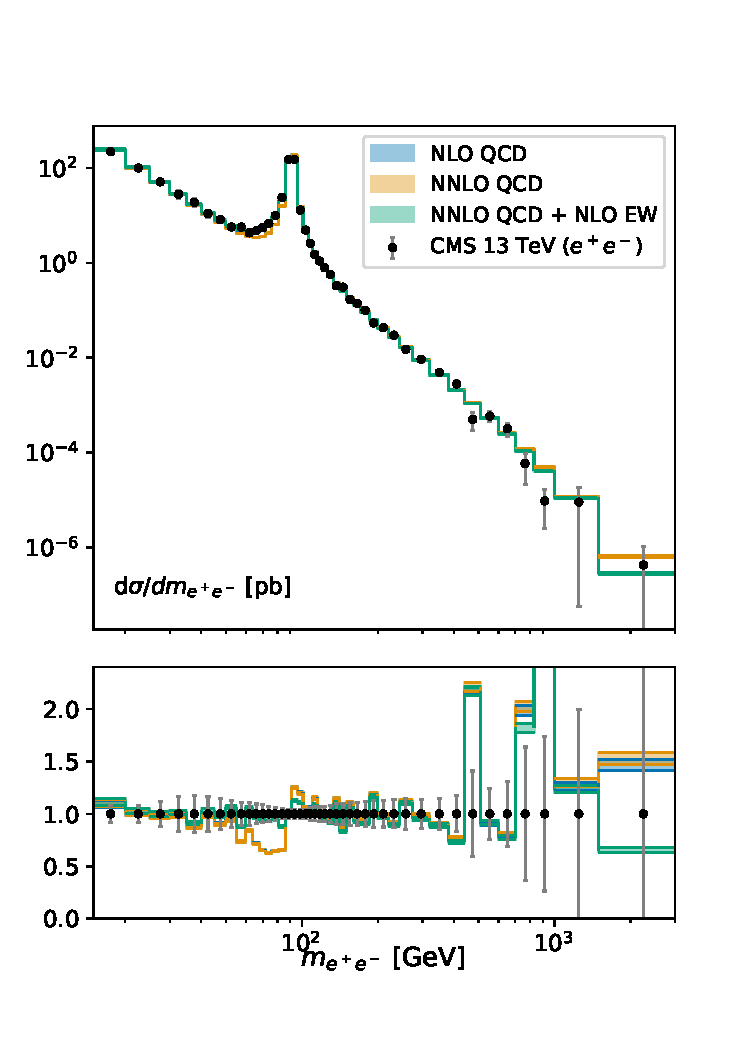
\includegraphics[width=0.49\textwidth]{dy_figures/cms13_electron_thpred_w_pdf_errs.pdf}
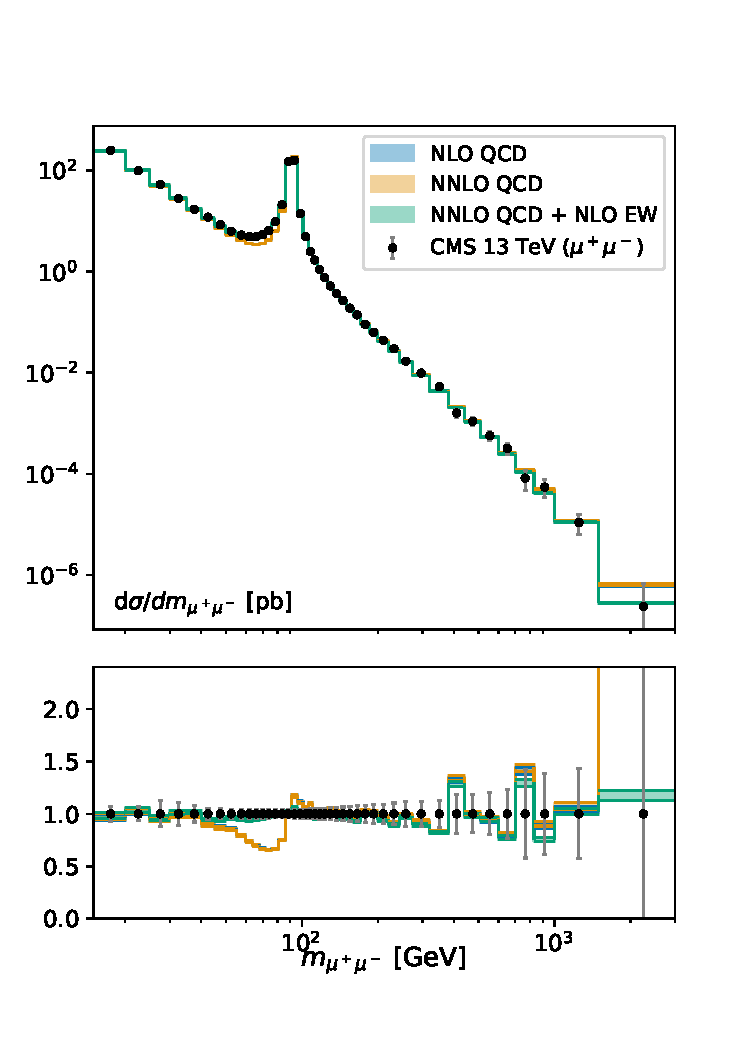
\includegraphics[width=0.49\textwidth]{dy_figures/cms13_muon_thpred_w_pdf_errs.pdf}
\caption{\small Comparison of the CMS Drell-Yan
  13 TeV data with the corresponding theoretical calculations at different
  perturbative orders as a function of the
  dilepton invariant mass $m_{\ell\ell}$ in the dielectron (left)
  and dimuon (right panel) final states.
  %
  The bottom panels display the ratio of the theory calculations
  to the central value of the experimental data.
  %
  We display the sum in quadrature of the experimental uncertainties, and the error
  band in the theory predictions correspond to the one-sigma PDF uncertainties.
  \label{fig:dysm}}
\end{figure}
%%%%%%%%%%%%%%%%%%%%%%%%%%%%%%%%%%%%%%%%%%%%%%%%%%%%%%%%%%%%%%%%%%%%%%%%%%%

Fig.~\ref{fig:dysm} displays a comparison between the CMS Drell-Yan distributions
at 13 TeV and the corresponding theoretical predictions as a function of the
dilepton invariant mass $m_{\ell\ell}$, separately for the dielectron
and dimuon final states.
  %
The theory calculations are presented at NLO QCD, NNLO QCD, and NNLO QCD combined with
NLO EW corrections, in all
cases with {\tt NNPDF3.1QED\_nnlo\_as\_0118} as input PDF set, to illustrate the
effect of the $K$-factors of Eq.~\eqref{def:kqcd} and
\eqref{def:kew}.
%
The CMS data are provided
in terms of dressed leptons, and hence final state radiation (FSR) QED effects must be included in the electroweak
corrections.
%
Accounting for these effects is essential to improve the agreement
between theory and data in the region below the $Z$-mass peak.
%
NLO electroweak corrections are also important in the high-energy tail in $m_{\ell\ell}$,
where they are driven by the interplay between (negative) virtual EW effects
and (positive) photon-initiated contributions.

A quantitative assessment of the agreement between theoretical predictions and experimental 
data for the high-mass DY datasets listed in Table~\ref{tab:data-high-mass}
is presented in Table~\ref{tab:dysm}, which collects the  values of the $\chi^2$ per data point
evaluated using the full information on correlated systematics
provided by the experimental covariance
matrix
\begin{equation}
  \label{eq:chi2}
\chi^2=\frac{1}{n_{\rm dat}}\sum_{i,j=1}^{n_{\rm
    dat}}(D_i-T_i)\,({\rm cov}^{-1})_{ij}\, (D_j-T_j),
\end{equation}
where $T_i$ are the theoretical predictions, $D_i$ the central value
of the experimental data and where the multiplicative uncertainties in
the experimental covariance matrix $({\rm cov}_{ij})$ are treated using the $t_0$ prescription as explained in Sect.~\ref{sec:the_loss_function} and in the references Refs.~\cite{Ball:2009qv,Ball:2012wy}.
%
One can observe how in general the NNLO QCD corrections are relatively
small and that the NLO electroweak
ones can be significant, especially for observables presented 
in terms of dressed leptons (such as the CMS 13 TeV ones) and are required to achieve a good description of the Drell-Yan
data in the whole kinematical range available.
%
Note that the input PDF sets used for these calculations include 
only a subset of these Drell-Yan measurements, in particular only the 7 TeV measurements, 
for which the data-theory agreement is comparable to the one observed in~\cite{Ball:2017nwa}.

The data-theory agreement before including the 
8 TeV and 13 TeV data in the PDF fit is generally good, once EW corrections 
are included, with the exception of the CMS 13 TeV data in the 
$e^+e^-$ channel, for which the $\chi^2$ per data point remains above 2.
%
As can be
observed in Fig.~\ref{fig:dysm}, the dielectron invariant mass distribution
in this channel presents dips at about
500 GeV and 900 GeV which are not present in the $\mu^+\mu^-$ channel.
%
These dips are the origin of this worse data-theory agreement,
which is partially reduced once the dataset is included in the fit
(see Sect.~\ref{sec:fitsettings}). 
We have verified that excluding this dataset from the fit does not 
change the results of the analysis, and therefore decided to keep it.
Further experimental analysis based on the full Runs II and III
datasets will tell whether the dips in the distributions in the
electron invariant mass will stay. 

%%%%%%%%%%%%%%%%%%%%%%%%%%%%%%%%%%%%%%%%%%%%%%%%%%%%%%%%%%%%%%%%%%%%%%%%%%%%%
\begin{table}[t]
  \renewcommand{\arraystretch}{1.40}
  \small
  \begin{center}
\begin{tabular}{c c c| c c c}
\toprule       
\multirow{3}{*}{Dataset} & \multirow{3}{*}{Final state} &  \multirow{3}{*}{$n_{\rm dat}$}    &  \multicolumn{3}{c}{$\chi^2/n_{\rm dat}$}   \\
      &  &      &  \multirow{2}{*}{NLO QCD}
           & \multirow{2}{*}{NNLO QCD}
& NNLO QCD \\
&  &      &  
           & 
& + NLO EW\\
\midrule
ATLAS 7 TeV  & $e^+e^-$            & 13  & 1.45  & 1.77  & 1.73 \\
ATLAS 8 TeV  & $\ell^+\ell^-$      & 46  & 1.67  & -     & 1.20 \\
\midrule
CMS 7 TeV    & $\mu^+\mu^-$        & 127 & 3.40  & 1.27  & 1.54 \\
CMS 8 TeV    & $\ell^+\ell^-$      & 41  & 2.22  & 2.21  & 0.70 \\
\midrule
CMS  13 TeV  & $\ell^+\ell^-$      & 43  & 18.7  & 19.7  & 1.91 \\
CMS  13 TeV  & $e^+e^-$            & 43  & 9.16  & 9.45  & 2.32 \\
CMS 13 TeV   & $\mu^+\mu^+$        & 43  & 15.7  & 15.8  & 0.81 \\
\bottomrule
\end{tabular}
\end{center}
  \caption{\label{tab:dysm}\small The values of the $\chi^2$ per data point
    evaluated for the  high-mass DY datasets listed in Table~\ref{tab:data-high-mass},
    using theoretical predictions computed at different perturbative accuracy.
    %
    The PDF sets used here are {\tt NNPDF31\_nlo\_as\_0118}, {\tt
    NNPDF31\_nnlo\_as\_0118} and {\tt NNPDF31\_nnlo\_as\_0118\_luxqed} for
    the NLO QCD, NNLO QCD and NNLO QCD + NLO EW predictions respectively.
    %
    For CMS 13 TeV, where different final states are available, we indicate the
    $\chi^2$ values for each of them.
    %
    For the ATLAS 8 TeV data, we only evaluated the combined
    NNLO QCD + NLO EW correction, and hence the  pure NNLO QCD result is not given.
  }
\end{table}
%%%%%%%%%%%%%%%%%%%%%%%%%%%%%%%%%%%%%%%%%%%%%%%%%%%%%%%%%%%%%%%%%%%%%%%%%%%%%

\paragraph{SMEFT corrections to the DIS structure functions.} In this chapter, we augment the SM calculations of the high-$Q^2$ DIS
reduced cross sections discussed in Ref.~\cite{Carrazza:2019sec} and
the high-mass Drell-Yan cross sections listed in
Table~\ref{tab:data-high-mass} with the effects of dimension-six SMEFT operators following the benchmark scenario presented in
Sect.~\ref{sec:dy_scenarios}.

Beginning with a discussion of DIS, the SMEFT corrections to the 
neutral-current deep-inelastic structure 
functions $F_2, F_3$ in the benchmark
scenario of Sect.~\ref{sec:dy_scenarios} are obtained by means of a direct
calculation in perturbation theory.
%
In order to determine these corrections, we rewrite Eq.~(\ref{eq:WYWarsaw})
as the linear combination of four-fermion operators of the form
$\bar{q}_{\lambda} \gamma^{\mu} q_{\lambda} \bar{\ell}_{\lambda'} \gamma_{\mu} \ell_{\lambda'}$,
where $q_\lambda$ is a quark field of helicity $\lambda$ (with $\lambda = +1$ for a
right-handed field and $\lambda=-1$ for a left-handed field) and $\ell_{\lambda^\prime}$ is a
lepton field of helicity $\lambda'$.
%
The relevant operators for the $\hat{Y}$ parameter
are already of this form in Eq.~(\ref{eq:WYWarsaw}).
%
For the $\hat{W}$ parameter,
the associated operators can be expanded explicitly as:
\begin{align}
\label{eq:WYfourfermion}
\mathcal{L}_{\rm SMEFT} \supset   &-\frac{g^2 \hat{W}}{4 m_W^2}  \sum_{i=1}^{3} \Bigg(\bar{e}_L^i \gamma^{\mu} e_L^i\bar{u}_L^i \gamma_{\mu} u_L^i - \bar{e}_L^i \gamma^{\mu} e_L^i \bar{d}_L^i \gamma_{\mu} d_L^i \\&- \bar{\nu}_L^i \gamma^{\mu} \nu_L^i \bar{u}_L^i \gamma_{\mu} u_L^i + \bar{\nu}_L^i \gamma^{\mu} \nu_L^i \bar{d}_L^i \gamma_{\mu} d_L^i  \Bigg), \nonumber
\end{align}
where the index $i$ runs over generations, and the flavour-changing contributions have been dropped since they only contribute to low energy CC structure functions.

The EFT corrections to the DIS structure functions induced by a specific four-fermion operator of the form:
\begin{equation}
\mathcal{L}_{\rm SMEFT} \supset \frac{c_{\lambda\lambda'}^{q\ell}}{\Lambda^2} \bar{q}_{\lambda} \gamma^{\mu} q_{\lambda} \bar{\ell}_{\lambda'} \gamma_{\mu} \ell_{\lambda'}
\end{equation}
can be shown (by a direct calculation in the parton model, as in Sect.~\ref{sec:factorisation}) to be given by:
\begin{align}
\Delta F_2(x,Q^2) &=  \frac{c_{\lambda\lambda'}^{qe}}{\Lambda^2}  \frac{Q^2  }{2e^2} \left( e_q - K_Z \left(V^e - \lambda' A^e\right)\left( V^q - \lambda A^q \right)  \right) \left( xf_q(x,Q^2) + xf_{\bar{q}}(x,Q^2) \right), \nonumber\\[1.5ex]
\Delta F_3(x,Q^2) &=-  \frac{c_{\lambda\lambda'}^{qe}}{\Lambda^2} \frac{Q^2}{2e^2} \left( \lambda \lambda' e_q - K_Z \left( \lambda' V^e - A^e \right) \left( \lambda V^q - A^q \right)\right) \left( f_q(x,Q^2) - f_{\bar{q}}(x,Q^2) \right),\nonumber
\end{align}
where $e$ is the positron charge, $e_q$ is the charge on the quark $q$ in units of the positron charge, $\theta_W$ is the Weinberg angle, and $K_Z = Q^2/\sin^2(2\theta_W)(Q^2 + m_Z^2).$
The vector and axial couplings are given by $V^e = -\frac{1}{2} +
2\sin^2(\theta_W)$, $A^e = -\frac{1}{2}$, $V^q = I_3^q -
2\sin^2(\theta_W)e_q$ and $A^q = I^q_3$,
where $I_3^q$ is the third
component of the quarks' weak isospin. These formulae are the natural
generalisations of those derived in~\cite{Carrazza:2019sec}, where only right-handed four-fermion
operators were considered.
%
Taking combinations of these DIS structure-function corrections according to
Eq.~(\ref{eq:WYWarsaw}) for the $\hat{Y}$ parameter and to Eq.~(\ref{eq:WYfourfermion}) for the $\hat{W}$ parameter
yields the sought-for EFT corrections for DIS observables.

This calculation has been implemented in {\tt APFEL}~\cite{Bertone_2014} following the strategy 
presented in~\cite{Carrazza:2019sec}. FK tables are produced from {\tt
  APFEL}~\cite{Bertone:2016lga} and then used to evaluate the DIS $K$-factors
defined in Eq.~\eqref{eq:theory_k_fac_app3}. Furthermore, we have used {\tt APFEL} to
include the higher-order QCD corrections in the SMEFT sector, so that in fact Eq.~(\ref{eq:theory_k_fac_app3})
holds exactly for the DIS $K$-factors in our study.

%%%%%%%%%%%%%%%%%%%%%%%%%%%%%%%%%%%%%%%%%%%%%%%%%%%%%%%%%%%%%%%%%%%%%%%% 
\begin{figure}[t]
\centering
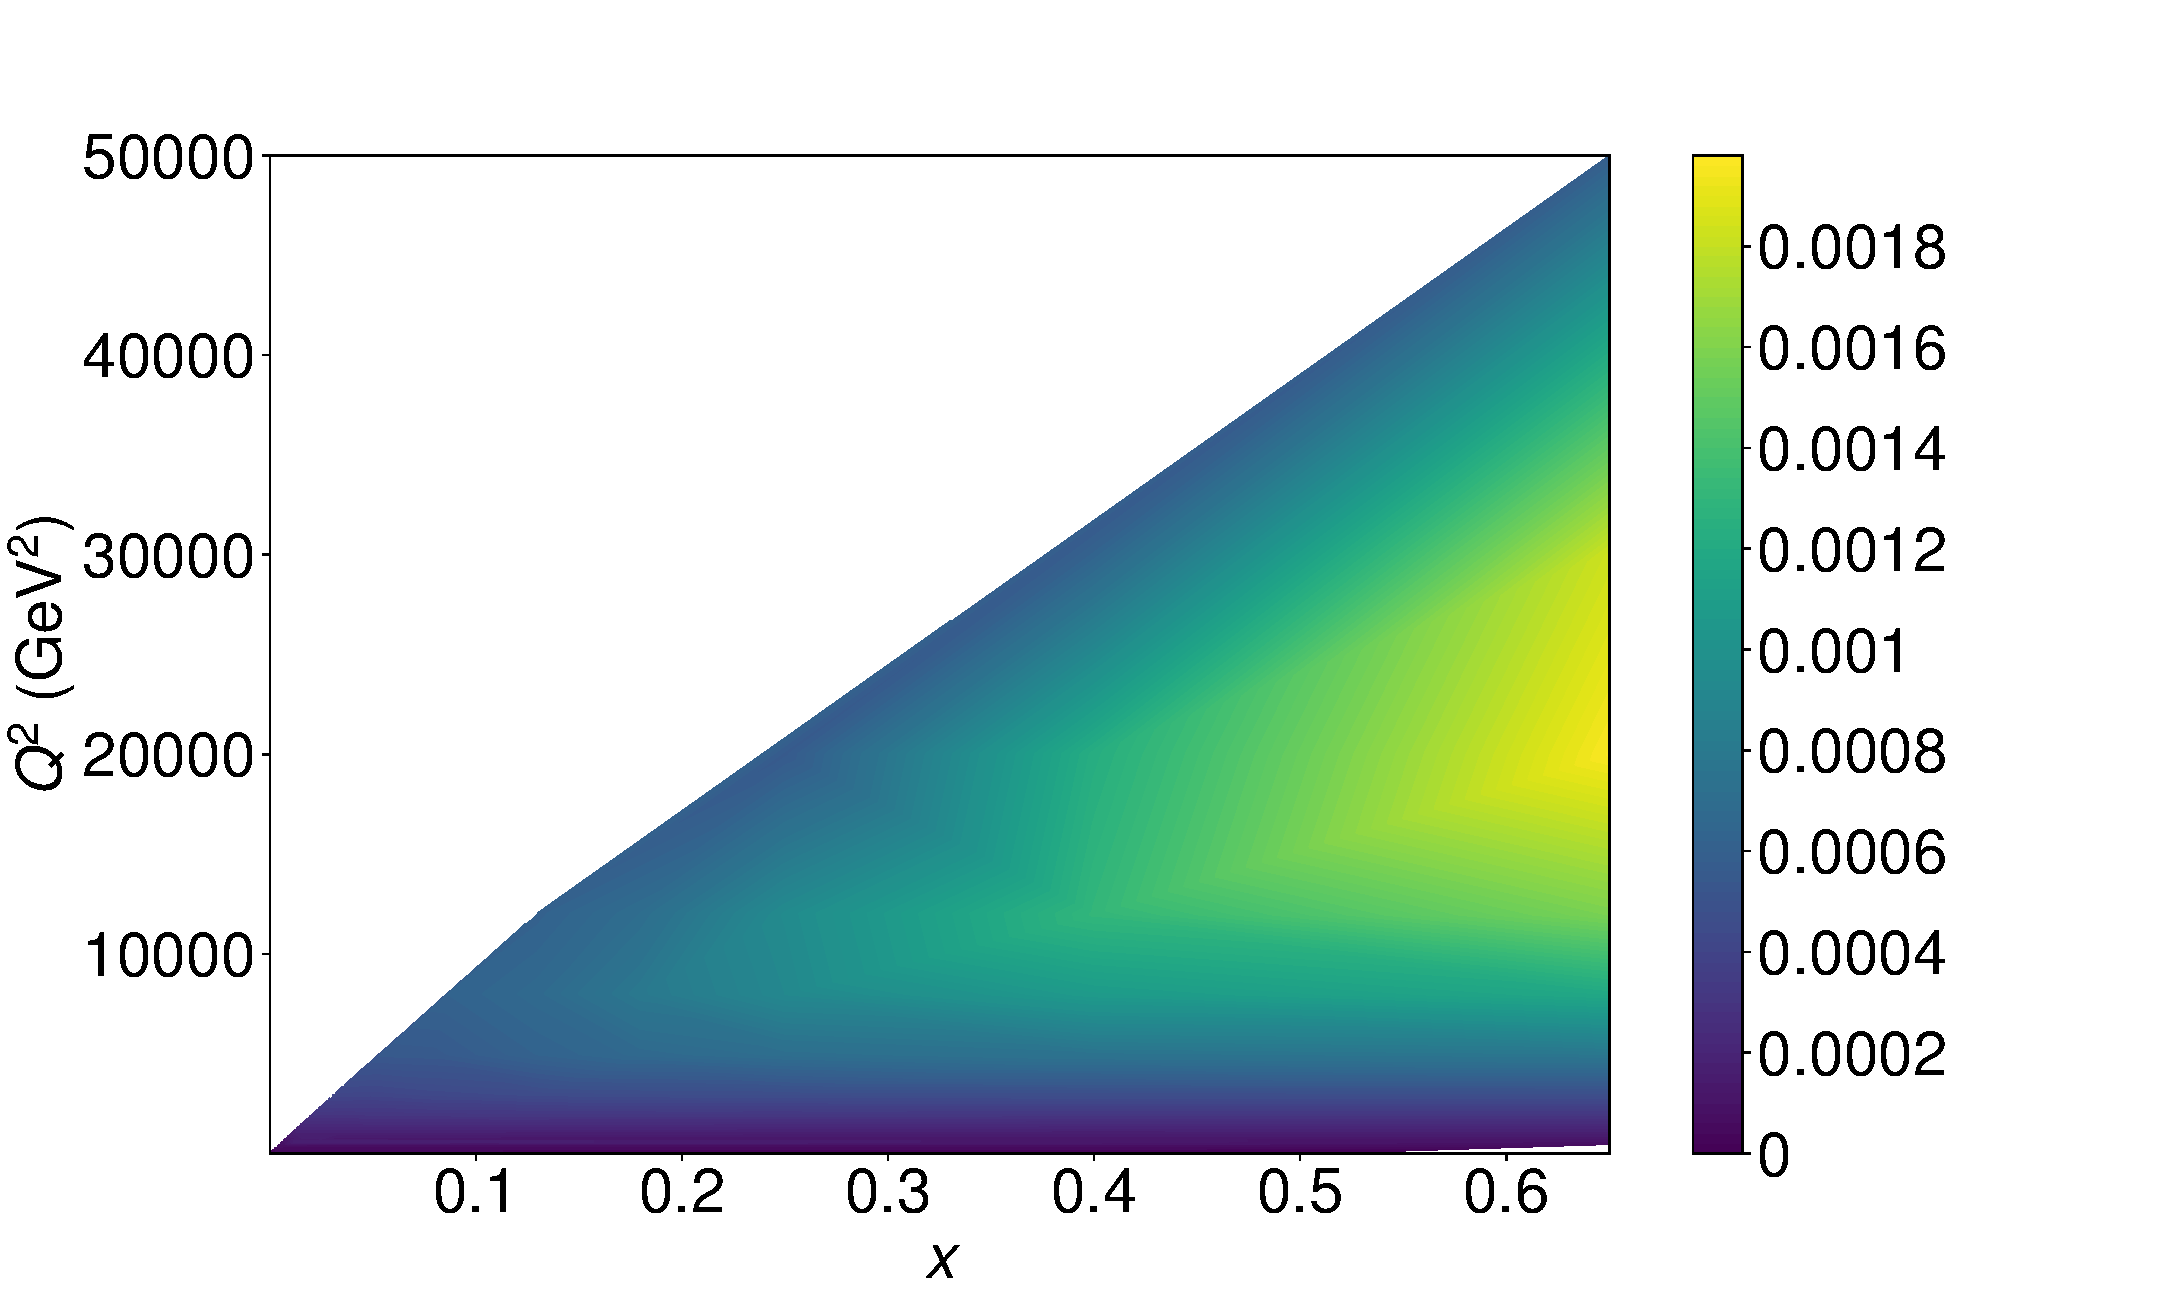
\includegraphics[width=0.49\textwidth]{dy_figures/disWinterp.pdf}
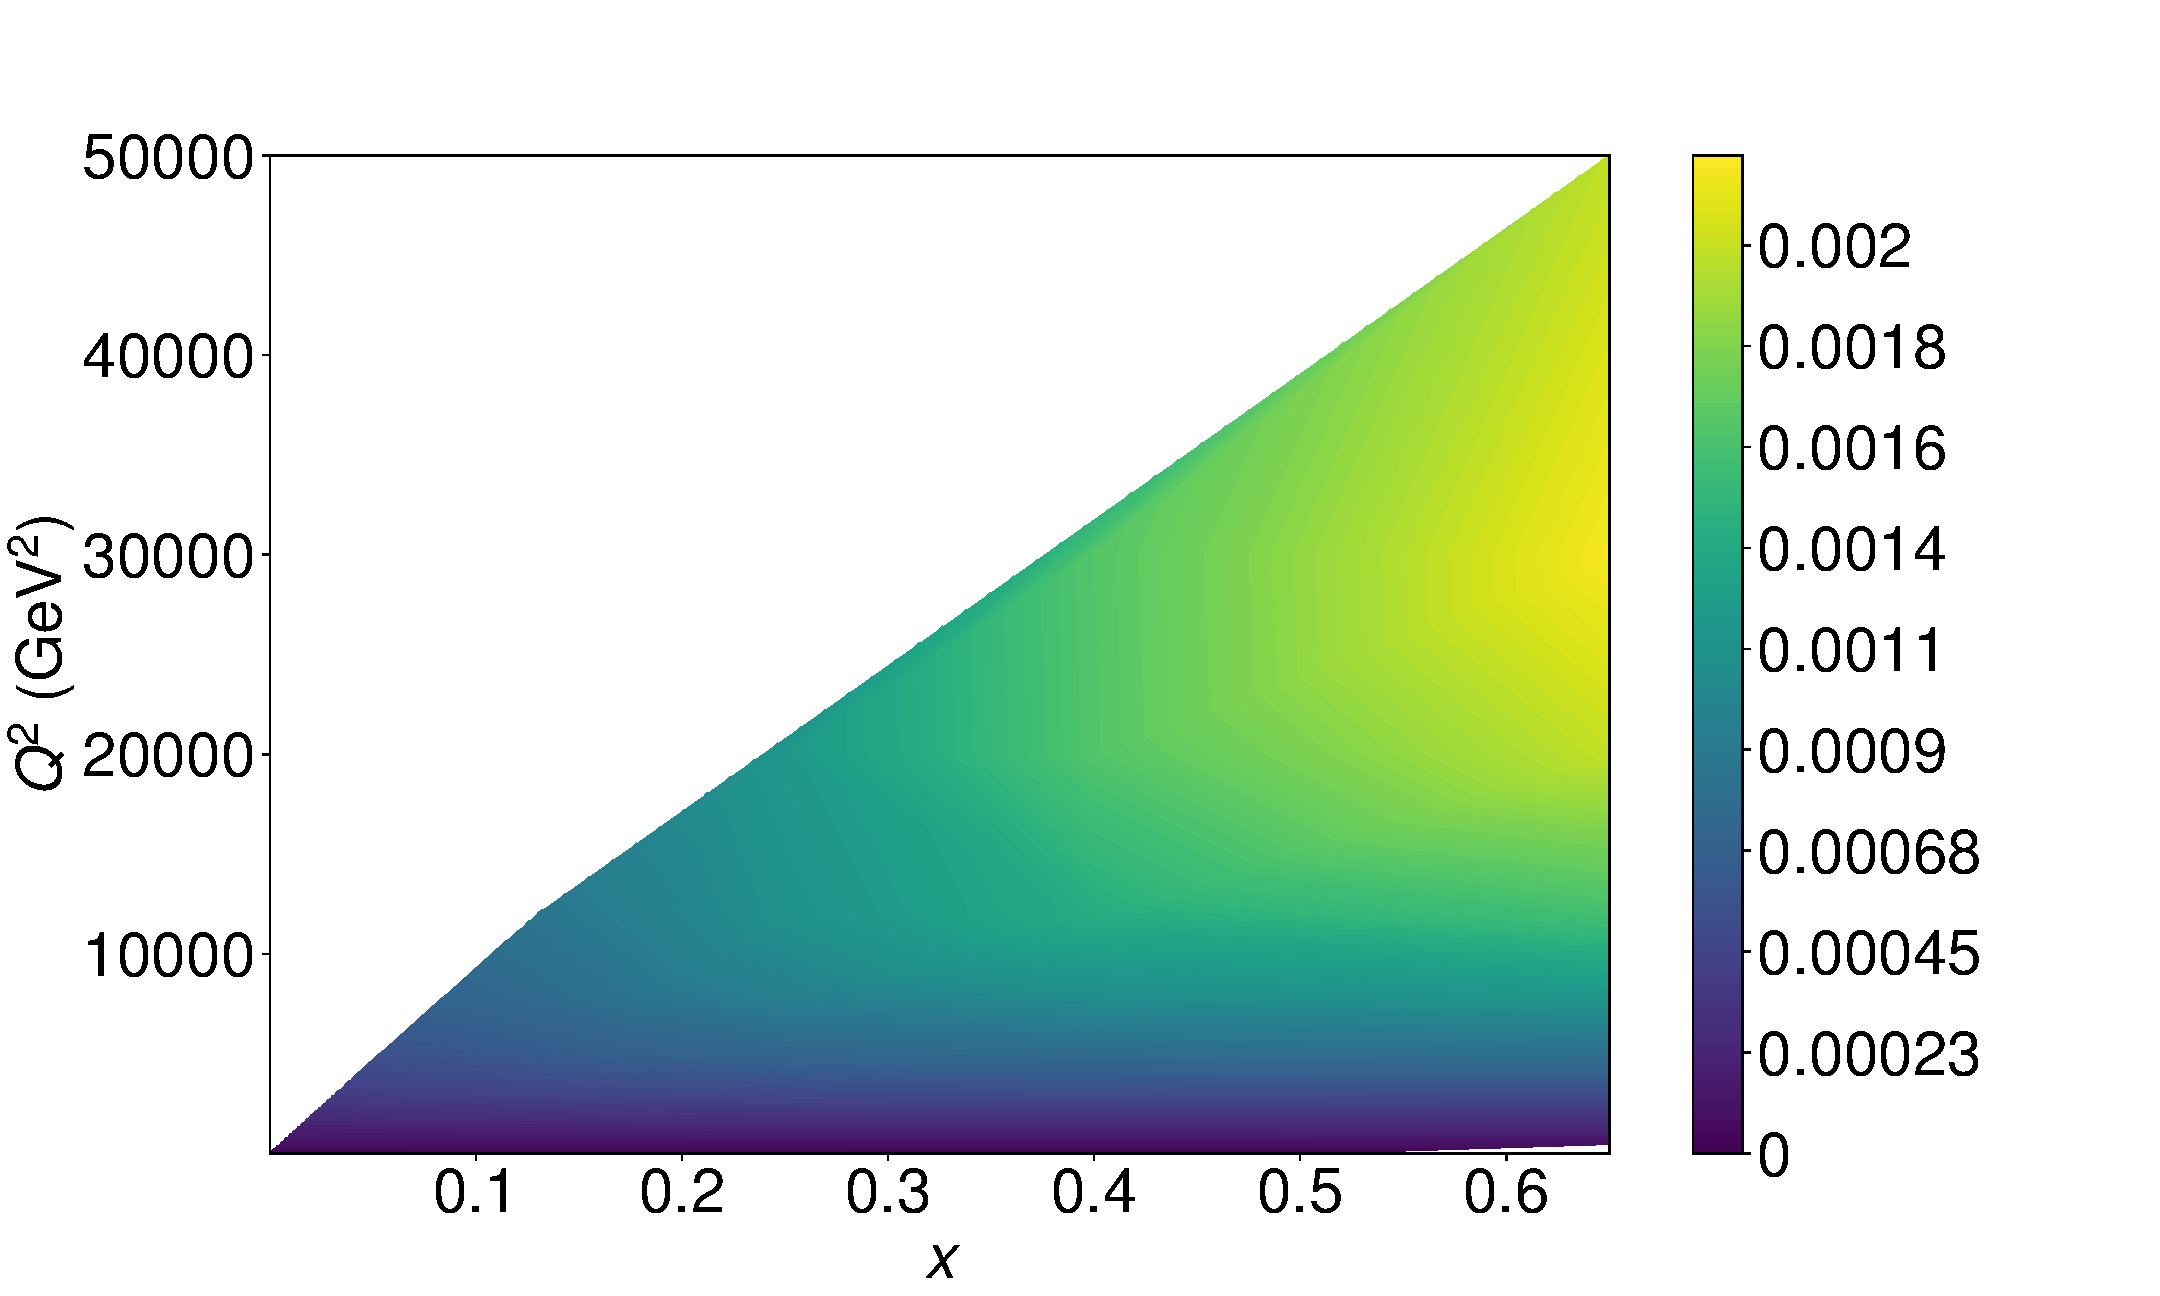
\includegraphics[width=0.49\textwidth]{dy_figures/disYinterp.pdf}\\
\caption{\small Contour maps indicating the value of the EFT correction, $K_{\rm EFT}(\hat{W},\hat{Y})$$-$$1$ in Eq.~(\ref{eq:theory_k_fac}),
  for the DIS reduced cross sections as a function of $x$ and $Q^2$ for two
  representative values of the EFT parameters: $\hat{W}=-10^{-4}$ (left panel) and $\hat{Y}=-10^{-4}$
  (right panel).
  \label{fig:dissmeft}}
\end{figure}
%%%%%%%%%%%%%%%%%%%%%%%%%%%%%%%%%%%%%%%%%%%%%%%%%%%%%%%%%%%%%%%%%%%%%%%%%

Fig.~\ref{fig:dissmeft} displays contour maps indicating the EFT correction, $K_{\rm EFT}(\hat{W},\hat{Y})$$-$$1$ in Eq.~(\ref{eq:theory_k_fac}),
  for the DIS reduced cross sections (which include both $F_2$ and $xF_3$) as a function of $x$ and $Q^2$ for two
  representative values of the EFT parameters, $\hat{W}=-10^{-4}$ and $\hat{Y}=-10^{-4}$.
  %
  These maps should be compared with Fig.~1 of~\cite{Carrazza:2019sec}, which considered
   different EFT scenarios.
  %
  We find that the overall effect of
  non-zero $\hat{W}$ and $\hat{Y}$ parameters is rather small, well below the percent level
  even for the highest bins in $Q^2$ covered by the HERA data.
  %
  This comparison highlights how, in this benchmark EFT scenario, the constraints
  on the $\hat{W}$ and $\hat{Y}$ parameters will be completely
  dominated by the (high-mass) Drell-Yan cross sections.

\paragraph{SMEFT corrections for Drell-Yan distributions.}
Similarly to DIS, the SMEFT corrections are negligible for dilepton invariant masses of $m_{\ell\ell}\le 200$
GeV and hence we can safely adopt the SM calculations there. For the high-mass Drell-Yan distributions however,
we must include the SMEFT corrections, which are appreciable.

In a similar manner as for higher-order QCD and EW corrections, we can
define correction factors that encapsulate  the linear and quadratic modifications induced
by the dimension-six SMEFT operators.
%
Adopting an operator normalisation such that:
\begin{equation}
\label{eq:lagrangian}
\mathcal{L}_{\rm SMEFT} = \mathcal{L}_{\rm SM} + \sum_{n=1}^{n_{\rm op}} \frac{c_n}{v^2} \,\mathcal{O}_n \, ,
\end{equation}
with $n_{\rm op}$ indicating the number of operators that contribute to a given
benchmark scenario and $c_n$ being the (dimensionless) Wilson coefficient associated to $\mathcal{O}_n$,
the linear EFT corrections can be parametrised as:
%
\begin{equation}
  \label{eq:mult_k_fac_app1}
   R_{\rm SMEFT}^{(n)} \equiv \displaystyle \left( {\cal L}_{ ij}^{\rm NNLO} \otimes d\widehat{\sigma}_{ij,{\rm SMEFT}}^{(n)}\right)
 \big/ \left( {\cal L}_{ ij}^{\rm NNLO} \otimes d\widehat{\sigma}_{ij,{\rm SM}} \right) \, , \quad
 n=1\,\ldots, n_{\rm op} \, ,
\end{equation}
%
with ${\cal L}_{ ij}^{\rm NNLO}$ being the usual partonic luminosity evaluated at NNLO QCD, 
$d\widehat{\sigma}_{ij,{\rm SM}}$
the bin-by-bin partonic SM cross section, and $d\widehat{\sigma}_{ij,{\rm SMEFT}}^{(n)}$
the corresponding partonic cross section associated to the interference between 
$\mathcal{O}_n$ and the SM amplitude $\mathcal{A}_{\rm SM}$ when setting $c_n = 1$.
%
Likewise, the ratio encapsulating the quadratic effects is defined as:
%
\begin{equation}
  \label{eq:mult_k_fac_app2}
  R_{\rm SMEFT}^{(n,m)} \equiv \displaystyle \left( {\cal L}_{ ij}^{\rm NNLO} \otimes d\widehat{\sigma}_{ij,{\rm SMEFT}}^{(n,m)}\right)
  \big/ \left( {\cal L}_{ ij}^{\rm NNLO} \otimes d\widehat{\sigma}_{ij,{\rm SM}} \right) \, , \quad
 n,m=1\,\ldots, n_{\rm op} \, ,
\end{equation}
with the bin-by-bin partonic cross section
$d\widehat{\sigma}_{ij,{\rm SMEFT}}^{(n,m)}$ now being evaluated from the squared amplitude $\mathcal{A}_n\mathcal{A}_m$
associated to the operators $\mathcal{O}_n$ and $\mathcal{O}_m$ when $c_n = c_m = 1$.
%
The partonic cross sections in these ratios are computed at LO.
%
In terms of  Eqns.~(\ref{eq:mult_k_fac_app1}) and~(\ref{eq:mult_k_fac_app2}), we can define the EFT $K$-factors as:
\begin{equation}
 \label{eq:theory_k_fac}
  K_{\rm EFT}= 1+\sum_{n=1}^{n_{\rm op}} c_n R_{\rm SMEFT}^{(n)}
  +\sum_{n,m=1}^{n_{\rm op}} c_n c_m R_{\rm SMEFT}^{(n,m)} \, ,
\end{equation}
  which allow us to express a general Drell-Yan or DIS cross sections accounting for
  the dimension-six operators in Eq.~(\ref{eq:lagrangian}) as:
\begin{equation}
  \label{eq:theory_k_fac_app3}
  d\sigma_{\rm SMEFT} = d\sigma_{\rm SM}
  \times  K_{\rm EFT} \, 
\end{equation}
where the $ d\sigma_{\rm SM}$ is the state-of-the-art SM prediction
including NNLO QCD and NLO EW corrections.
%
In this approach, the SMEFT predictions inherit factorisable higher-order radiative correction~\cite{Greljo:2017vvb,Ricci:2020xre}. 
%
%
The SMEFT $K$-factors in Eq.~(\ref{eq:theory_k_fac}) are
precomputed before the fit using a reference SM PDF set and then kept fixed.
%
The effect of varying the input NNLO PDF in
Eqns.~(\ref{eq:mult_k_fac_app1}) and~(\ref{eq:mult_k_fac_app2})
is quantitatively assessed in App. C of Ref.~\cite{Greljo:2021kvv} and it
is found to be at the permil level.
As a result, this effect will be neglected in the following.

Fig.~\ref{fig:dysmeft} illustrates the size of the EFT corrections in
the benchmark scenario from Sect.~\ref{sec:dy_scenarios} by comparing
$(K_{\rm EFT}$$-$$1)$
with the relative experimental
  uncertainties  for the ATLAS 7 TeV, CMS 8 TeV,
  and CMS 13 TeV Drell-Yan $m_{\ell\ell}$ distributions.
  %
  We provide results for two representative points in the $(\hat{W}$, $\hat{Y})$
  parameter space, namely $(\hat{W}$, $\hat{Y})=(10^{-3},0)$ and $(0,10^{-3})$.
    %
  One can observe how for these values of $(\hat{W}$, $\hat{Y})$, 
and particularly for the ATLAS 8 TeV data, the SMEFT corrections
  to the Drell-Yan cross sections become comparable with the experimental uncertainties, 
  increasing steadily with $m_{\ell\ell}$.
  %

%%%%%%%%%%%%%%%%%%%%%%%%%%%%%%%%%%%%%%%%%%%%%%%%%%%%%%%%%%%%%%%%%%%%%%%%
\begin{figure}[t]
\centering
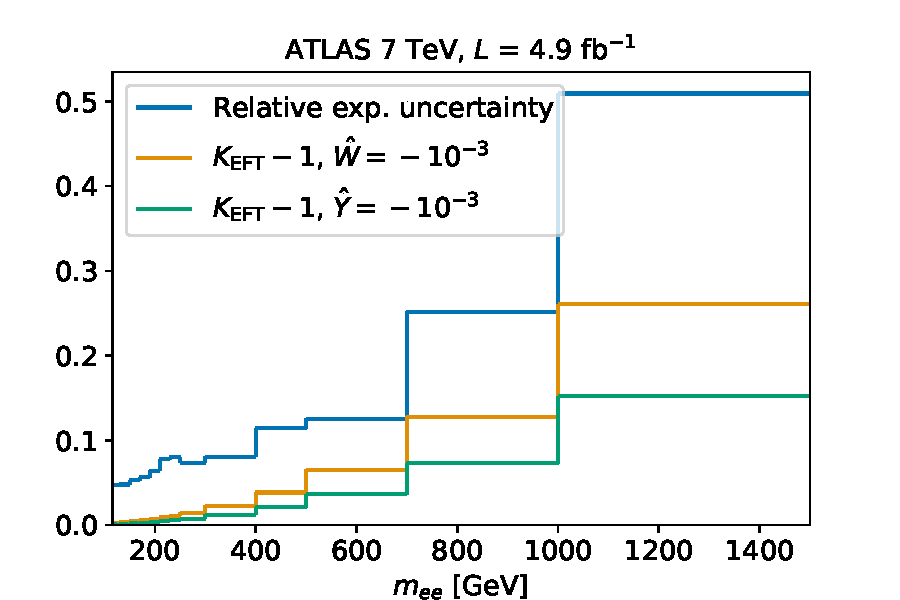
\includegraphics[width=0.49\textwidth]{dy_figures/atlas_7tev_kfacs.pdf}
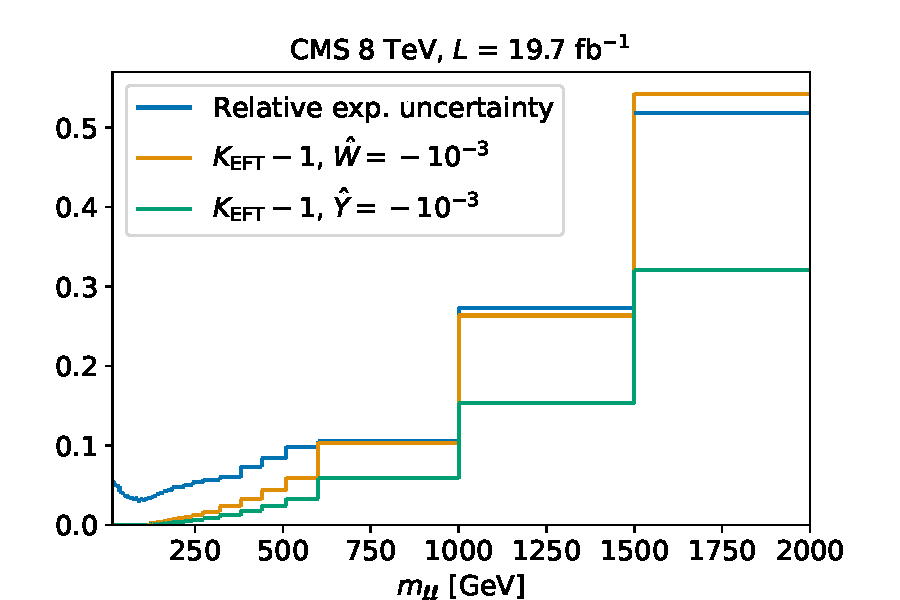
\includegraphics[width=0.49\textwidth]{dy_figures/cms_8tev_kfacs.pdf}\\
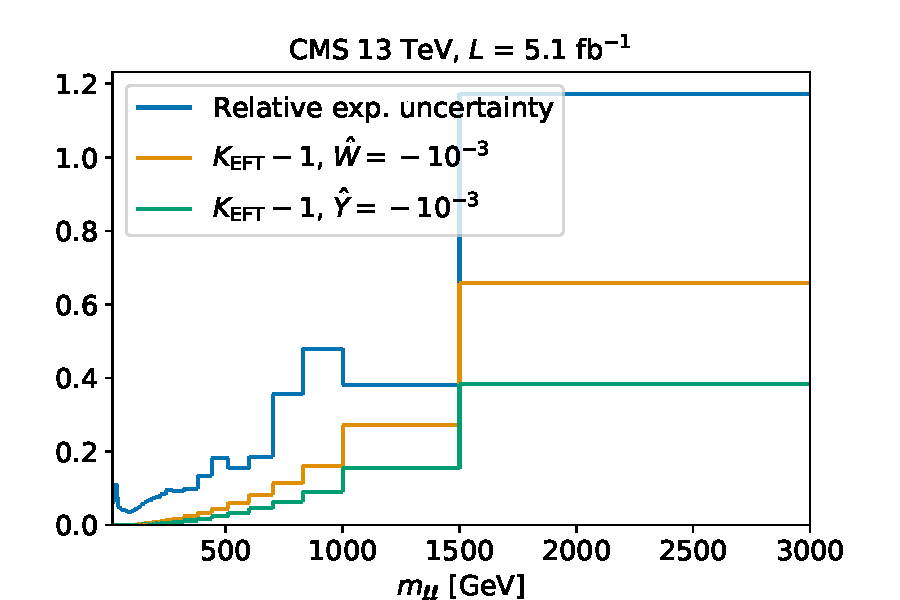
\includegraphics[width=0.49\textwidth]{dy_figures/cms_13tev_kfacs.pdf}
\caption{\small Comparison between the (relative) experimental
  uncertainties and the corresponding EFT corrections,
$K_{\rm EFT}(\hat{W},\hat{Y})$$-$$1$ in Eq.~(\ref{eq:theory_k_fac}),
  for the ATLAS 7 TeV, CMS 8 TeV,
  and CMS 13 TeV Drell-Yan $m_{\ell\ell}$ distributions,
  for two representative values of  $\hat{W}$ and $\hat{Y}$.
  \label{fig:dysmeft}}
\end{figure}
%%%%%%%%%%%%%%%%%%%%%%%%%%%%%%%%%%%%%%%%%%%%%%%%%%%%%%%%%%%%%%%%%%%%%%%%%


%%%%%%%%%%%%%%%%%%%%%%%%%%%%%%%%%%%%%%%%%%%%%%%%%%%%%%%%
%%%%%%%%%%%%%%%%%%%%%%%%%%%%%%%%%%%%%%%%%%%%%%%%%%%%%%%%

\subsection{Baseline SM PDFs}
\label{sec:fitsettings}
The settings for this baseline SM PDF fit used in this chapter are the same as those used in the strangeness study
of~\cite{Faura:2020oom}, itself a variant of NNPDF3.1~\cite{Ball:2017nwa}. As described in Sect.~\ref{sec:dy_dataset}, in this work we consider only DIS
and Drell-Yan datasets, with the latter augmented as compared to~\cite{Faura:2020oom} with the new high-mass
measurements indicated in Table~\ref{tab:data-high-mass}.

In general, the fit quality of the baseline SM PDF set
is similar to that of the global fit of~\cite{Faura:2020oom},
although the description of the CMS 13 TeV 
invariant mass distribution in the combined electron and muon 
channels remains sub-optimal. See App. B of Ref.~\cite{Greljo:2021kvv} for a complete discussion of the fit quality.

%%%%%%%%%%%%%%%%%%%%%%%%%%%%%%%%%%%%%%%%%%%%%%%%%%%%%%%%%%%%%%%%%%%%%%%%
\begin{figure}[H]
  \centering
  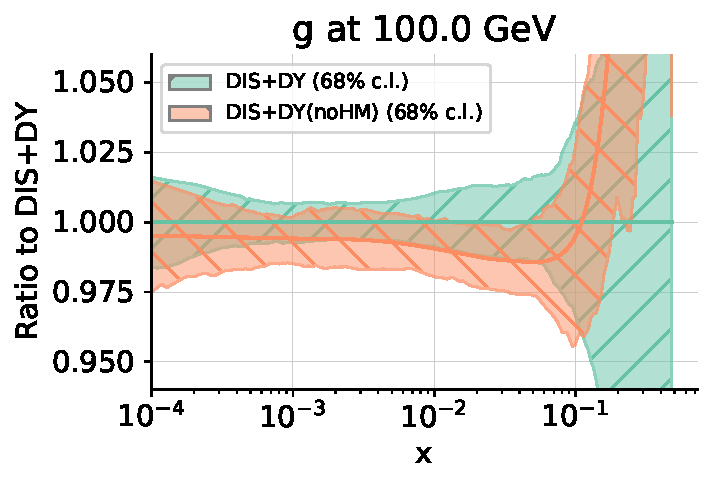
\includegraphics[width=0.32\textwidth]{dy_figures/HDMY_Bases0_PDFRanges_DistPDFs_plot_pdfs_g.pdf}
  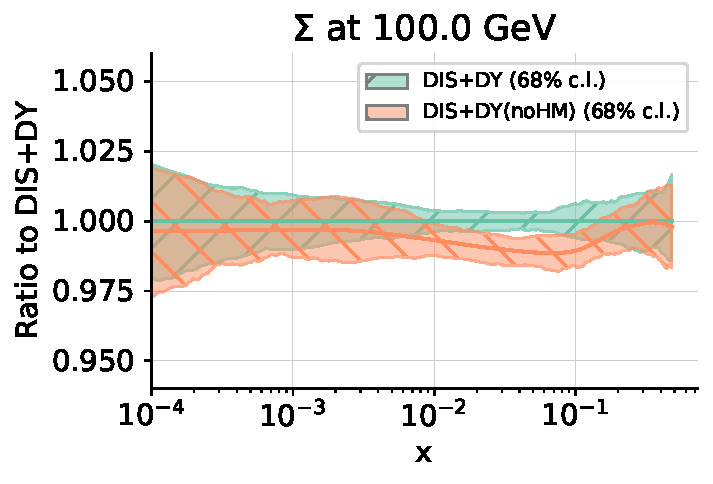
\includegraphics[width=0.32\textwidth]{dy_figures/HDMY_Bases0_PDFRanges_DistPDFs_plot_pdfs_Sigma.pdf}
  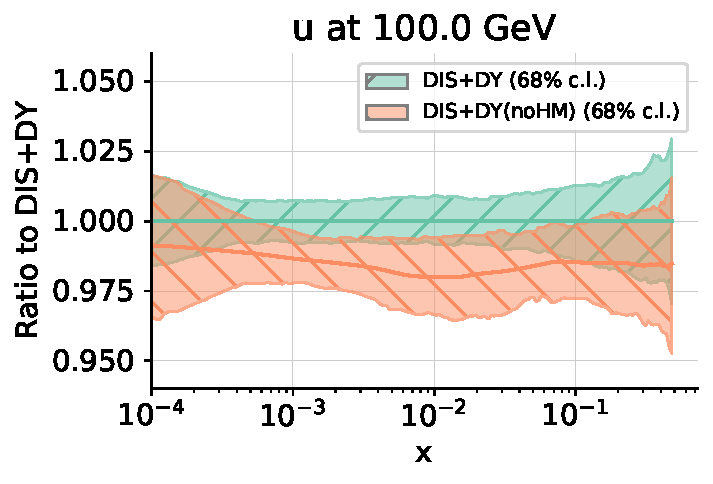
\includegraphics[width=0.32\textwidth]{dy_figures/HDMY_Bases1_PDFRanges_DistPDFs_plot_pdfs_u.pdf}
  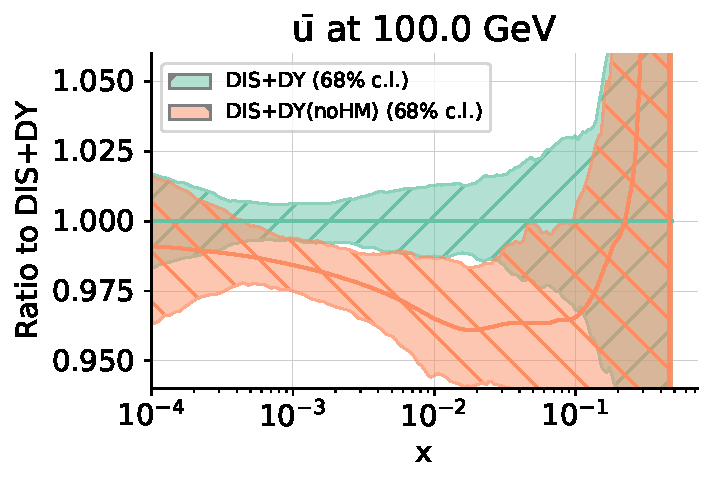
\includegraphics[width=0.32\textwidth]{dy_figures/HDMY_Bases1_PDFRanges_DistPDFs_plot_pdfs_baru.pdf}
  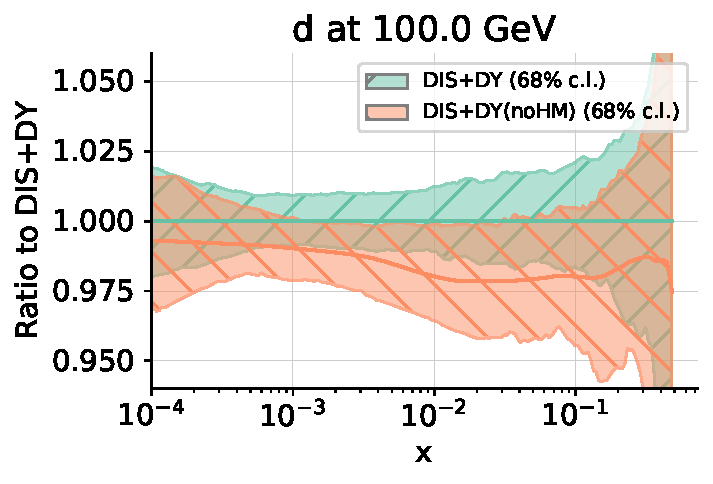
\includegraphics[width=0.32\textwidth]{dy_figures/HDMY_Bases1_PDFRanges_DistPDFs_plot_pdfs_d.pdf}
  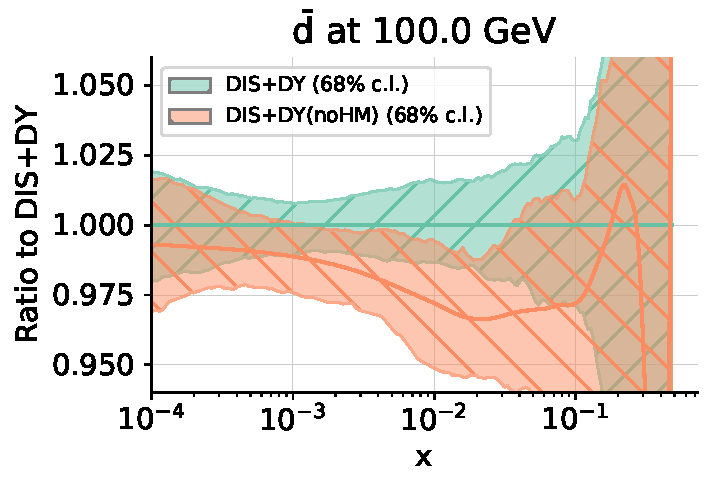
\includegraphics[width=0.32\textwidth]{dy_figures/HDMY_Bases1_PDFRanges_DistPDFs_plot_pdfs_bard.pdf}
  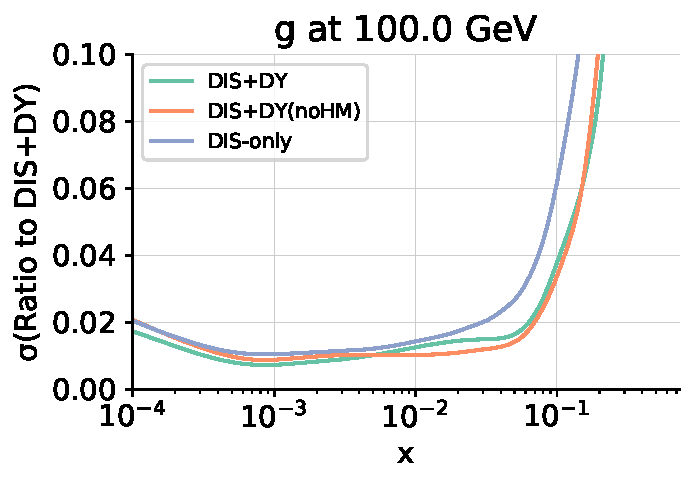
\includegraphics[width=0.32\textwidth]{dy_figures/HDMY_Bases0_UncRanges_UncPDFs_plot_pdf_uncertainties_g.pdf}
  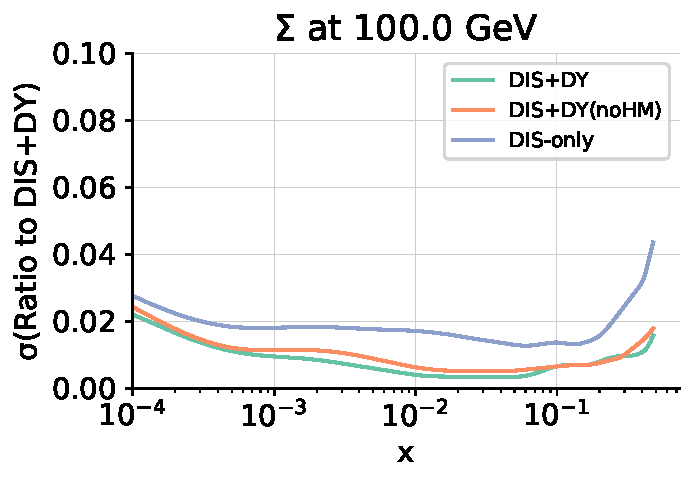
\includegraphics[width=0.32\textwidth]{dy_figures/HDMY_Bases0_UncRanges_UncPDFs_plot_pdf_uncertainties_Sigma.pdf}
  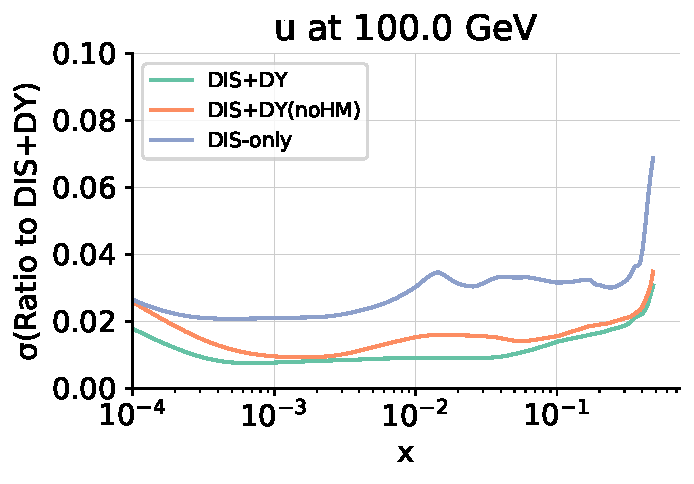
\includegraphics[width=0.32\textwidth]{dy_figures/HDMY_Bases1_UncRanges_UncPDFs_plot_pdf_uncertainties_u.pdf}
  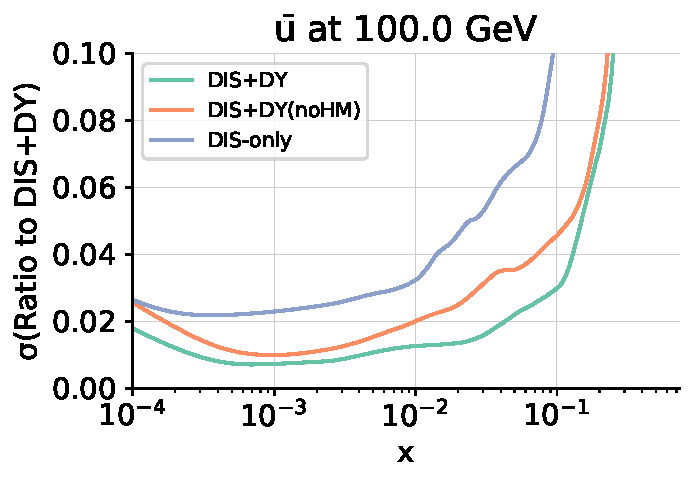
\includegraphics[width=0.32\textwidth]{dy_figures/HDMY_Bases1_UncRanges_UncPDFs_plot_pdf_uncertainties_baru.pdf}
  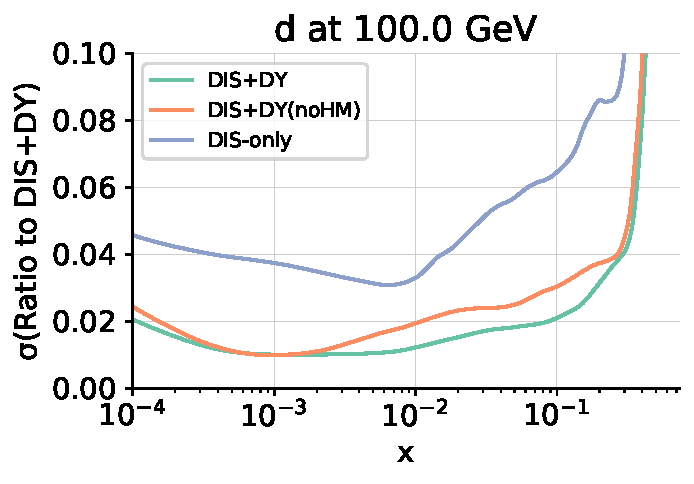
\includegraphics[width=0.32\textwidth]{dy_figures/HDMY_Bases1_UncRanges_UncPDFs_plot_pdf_uncertainties_d.pdf}
  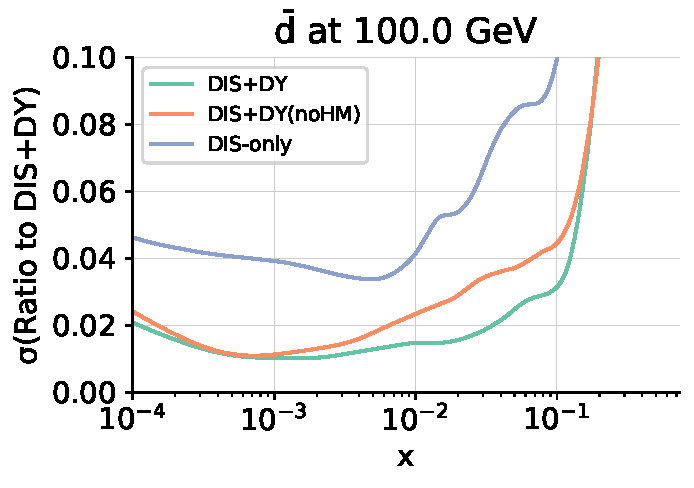
\includegraphics[width=0.32\textwidth]{dy_figures/HDMY_Bases1_UncRanges_UncPDFs_plot_pdf_uncertainties_bard.pdf}
  \caption{\small \small Comparison between the baseline SM PDF set of this work, labelled `DIS+DY', with
    the corresponding fit without high-mass DY data.
  We show results at $Q=100$ GeV for PDFs normalised to the central value of the baseline (upper) and
  for the relative PDF uncertainties (lower panels).
  %
  In the latter case, we also display the PDF uncertainties from the DIS-only fit.
  \label{fig:pdfplot-impactHMDY}}
\end{figure}
%%%%%%%%%%%%%%%%%%%%%%%%%%%%%%%%%%%%%%%%%%%%%%%%%%%%%%%%%%%%%%%%%%%%%%%%%

Fig.~\ref{fig:pdfplot-impactHMDY} displays a comparison
between this baseline SM PDF set, labelled `DIS+DY', with
the same fit but without any datapoints from the high-mass DY datasets
listed in Table~\ref{tab:data-high-mass}, labelled `DIS+DY (no HM)'.
%
 We show results at $Q=100$ GeV both for the PDFs normalised to the
 central value of the baseline and for the relative PDF
 uncertainties. In the latter case we also display the PDF uncertainties from a corresponding DIS-only fit.
The latter comparison shows that the DY cross sections significantly reduce
the PDF uncertainties of the DIS-only fit.
%
The addition of the high-mass DY data leads to a visible  
uncertainty reduction in the $0.005 \lesssim x\lesssim  0.3$ region
as compared to the `DIS+DY(noHM)' reference as well an upwards shift
of the up and down quarks and antiquark PDF.

We therefore find that the available high-mass DY data can
have an appreciable impact on the light quark and antiquark PDFs,
despite the fact that in terms of Run II data our  analysis is restricted to a single low-luminosity 
 high-mass DY dataset.
%
Yet more stringent constraints on the PDFs are expected from the measurements based
on the full Run II and Run III datasets,
as well as from those to be provided by the HL-LHC~\cite{Khalek:2018mdn}.
%
We study the anticipated impact of the HL-LHC measurements in
Sect.~\ref{sec:hllhc}.

%%%%%%%%%%%%%%%%%%%%%%%%%%%%%%%%%%%%%%%%%%%%%%%%%%%%%%%%%%%%%%%%%%

\subsection{Methodology for the simultaneous PDF and EFT fits}
\label{eq:jointfits}

Let us denote by ${\mathbf{c}}=(c_1,c_2,\ldots,c_{N_{\rm op}})$ the array containing
the Wilson coefficients associated to the $N_{\rm op}$ dimension-six
operators contributing to a given SMEFT scenario, where $c_n$ are
defined as in Eq.~\eqref{eq:lagrangian}. 
  %
For each point ${\mathbf{c}_i}$ in the scan of the EFT parameter space, we evaluate
the Drell-Yan and the DIS cross sections as described in Sect.~\ref{sec:theory}.
%
Subsequently, we determine the best-fit
PDFs associated to ${\mathbf{c}_i}$ by means of the standard NNPDF methodology, which
determines the minimum of the $\chi^2$ in the space of the PDF
parameters (subject to cross-validation, to avoid overlearning).
%
We note that this $\chi^2$, defined in
Eq.~\eqref{eq:chi2}, keeps fully into account the experimental
systematic correlations among all the
measurements $D_i$ included in the PDF analysis. 

This procedure results in a sampling of the $\chi^2$ values
in the EFT parameter space, which we denote by $\chi_{\rm eftp}^2({\mathbf{c}_i})$
(as in: EFT-PDFs).
%
Alternatively, one could also evaluate the same DIS and DY cross sections using instead
the baseline SM PDF set, ending up with  $\chi^2$ values which we denote by $\chi_{\rm smp}^2({\mathbf{c}_i})$
(as in: SM-PDFs).
%
The comparison between the resulting bounds on the EFT coefficients
obtained  from 
$\chi_{\rm eftp}^2({\mathbf{c}_i})$
and from $\chi_{\rm smp}^2({\mathbf{c}_i})$ quantifies the relevance of
producing consistent joint determinations of PDFs and Wilson coefficients
when studying EFTs in high-energy tails.
%
This strategy follows the one adopted in the proof-of-concept DIS-only
study~\cite{Carrazza:2019sec}, now extended to LHC processes.

Close enough to a local minimum $\chi_0^2=\chi^2\left( \mathbf{c}^{(0)}\right)$ associated with best-fit values $\mathbf{c}^{(0)}$,
the $\chi^2$ as a function of the EFT coefficients can be approximated by a quadratic form
\begin{equation}
\label{functional-form}
\chi_i^2 \equiv \chi^2(\mathbf{c}_i) = \chi_0^2 +
\sum_{n,m=1}^{N_{\rm op}}\left( c_{n,i} - c^{(0)}_n\right)  H_{nm} 
    \left( c_{m,i} - c^{(0)}_m\right)\, ,
\end{equation}
with $H_{nm}$ being the usual Hessian matrix in the EFT parameter space.
%
Restricting the EFT calculations to their linear, $\mathcal{O}\left( \Lambda^{-2}\right)$, contributions, Eq.~(\ref{functional-form})
becomes exact
in the case of $\chi_{\rm smp}^2({\mathbf{c}_i})$ (where cross sections are
evaluated with SM PDFs).
%
The reason is that in this case
all dependence on the EFT coefficients is encoded in the partonic cross sections.

However, this is not true for $\chi_{\rm eftp}^2({\mathbf{c}_i})$, since now there will be a (non-linear) EFT back-reaction
onto the PDFs and hence Eq.~(\ref{functional-form}) is only valid up
to higher orders in the EFT expansion, even if the EFT cross sections themselves are evaluated in the linear
approximation.
%
Eq.~(\ref{functional-form}) can thus be only considered a reasonable approximation in the case that the SMEFT PDFs are not
too different from their SM counterparts.

Hence, if we work with linear EFT calculations,
provided the sampling in the EFT parameter space is sufficiently broad and fine-grained,
and that the EFT-induced distortion on the PDFs is moderate,
we can extract the parameters $\chi^2_0$ and
${\mathbf{c}}^{(0)}$ and the Hessian matrix $H$ using least-squares regression from Eq.~(\ref{functional-form}),
using $\chi^2_{\rm smp}$ for the SM PDFs and  $\chi^2_{\rm eftp}$ for the SMEFT PDFs.
% 
The associated confidence level contours are determined by imposing
\begin{align}
  \label{eq:deltachi2def}
  \Delta\chi^2({\mathbf c}) \equiv \chi_i^2({\mathbf c})
  - \chi_0^2  = \sum_{n,m=1}^{N_{\rm op}}\left( c_{n} - c^{(0)}_n\right)  H_{nm} 
    \left( c_{m} - c^{(0)}_m\right) =\text{constant}\, ,
\end{align}
where this constant depends on the number of degrees of freedom.
%
For linear EFT two-parameter fits, such as those in the benchmark scenario,
 in the context of the HL-LHC projections we shall eventually consider, 
imposing Eq.~(\ref{eq:deltachi2def}) leads to elliptic
contours in the $( \hat{W},\hat{Y})$ plane.


To conclude this section, we give details on how we account for PDF
uncertainties and the statistical uncertainty associated to the finite
replica sample of the NNPDF Monte Carlo sets that we use here.

\paragraph{PDF uncertainty.} In
Sects.~\ref{sec:res1} and~\ref{sec:hllhc_joint_fits} we
will present bounds on the EFT parameters  using the SM PDFs
with and without the PDF uncertainties being accounted for.
%
In order to estimate these, we follow the procedure detailed above to
determine the confidence level intervals for the EFT parameters but now
using the $k$th Monte Carlo replica of the PDF set, rather than the central replica $k=0$
as done when PDF uncertainties are neglected.
%
One ends up with  $N_{\rm rep}$ values of
the upper and lower bounds:
\begin{equation}
\left[{\mathbf c}^{(k)}_{\rm min},{\mathbf c}^{(k)}_{\rm max}\right] \, ,\qquad k=1,\ldots,N_{\rm rep} \, ,
\end{equation}
and then the outermost bounds in the \(68\%\) envelope are considered to be the bounds
on the EFT parameters ${\mathbf c}$, now including the 1$\sigma$-PDF uncertainty.
%
This is very important to account for, given that in the case of the
bounds determined using $\chi^2_{\rm eftp}$, the PDF
uncertainty is already included by
construction, given that the Wilson coefficients are determined from the
global set of PDFs, exactly as in the case of the $\alpha_s$
determination from a global set of PDFs of
\cite{Lionetti:2011pw,Ball:2011us}. A more sophisticated way to
extract parameters such as $\alpha_s$ of the Wilson coefficients from
a global fit of PDFs, that includes the correlations between these parameters
and the PDFs, is given by the correlated replica method proposed in the more recent $\alpha_s$ determination in
\cite{Ball:2018iqk}. The latter would allow better accounting of the correlations
between Wilson coefficients and PDFs. However we do not use it here due to the fact that the correlations of the
PDFs with the Wilson coefficients are much smaller than those with the strong
coupling constant, and due to its large computational cost. This issue is addressed with the introduction of a new
methodology, presented in Chapter~\ref{chap:top}.

\paragraph{Methodological uncertainty.} In a simultaneous fit of PDFs and EFT coefficients,
for each set of Wilson coefficients \(\mathbf{c}_i\)
one has a PDF fit composed of \(N_\text{rep}\) Monte Carlo replicas.
%
The major methodological uncertainty is associated to  finite-\(N_\text{rep}\) effects, and
can be estimated by bootstrapping across the replicas, as explained in the $\alpha_s(m_Z)$
extraction of~\cite{Ball:2018iqk}.
%
Specifically, for each value of \(\mathbf{c}_i\)
we perform \(N_\text{res}\) re-samples of all \(N_\text{rep}\) replicas with replacement, and compute the theory predictions:
\begin{equation}
  \mathbf{T}^{\text{(res)}}_{i,lk} \, ,\quad
  \begin{matrix}
    l = 1,\dots,N_\text{res} \\
    k = 1,\dots,N_\text{rep}
  \end{matrix} \, ,
\end{equation}
such that there are \(N_\text{res}\) re-samples each composed of an \(N_\text{rep}\)-sized array
of theory predictions.
%
Since this re-sampling is done with replacement,
it differs from the original sample in that it contains  duplicates and missing values.
%
The average theory prediction is then obtained for each of these bootstrapped sets:
\begin{equation}
  \overline{\mathbf{T}}_{i,l} = \left<\mathbf{T}^\text{(res)}_{i,lk}\right>_\text{rep}\, ,
  \quad l = 1,\dots,N_{\text{res}} \, .
\end{equation}
These bootstrapped  theory predictions $\overline{\mathbf{T}}_{i,l}$ are used to evaluate the $\chi^2$ to data,
with the finite-size uncertainty given by the standard deviation across each bootstrap re-sample:
\begin{equation}
  \label{eq:finitesizechi2}
  \sigma_{\chi^2_i} = \text{std}\left(\chi^2_{i,l}\right)\Big|_\text{res}\, .
\end{equation}
A value of $N_\text{res}\simeq 10^4$ re-samples is found to be sufficient to achieve stable results
for the estimate of the finite-size uncertainties defined by Eq.~(\ref{eq:finitesizechi2}).



\section{Results from current Drell-Yan data}
\label{sec:res1}

In this section, we present results for the SMEFT PDFs extracted from DIS and Drell-Yan
data in the benchmark SMEFT scenario. We compare them with their SM counterparts at the level
of partonic luminosities
and assess how the bounds obtained on the $\hat{W}$ and $\hat{Y}$
parameters in this simultaneous SMEFT and PDF fit compare to those based on assuming SM PDFs.
We present results for one-dimensional fits where only one of the $\hat{W}$ or the $\hat{Y}$
parameter is allowed to be non-zero; the reason for this choice is that, in a fit including only high-mass neutral-current
Drell-Yan processes, there exists a flat direction when $\hat{W}$ and $\hat{Y}$ are varied
simultaneously, since both operators scale as $O(q^4)$ and thus cannot both be constrained by a single 1D distribution.
%
This degeneracy can only be lifted once high-mass charged-current DY data is included in the fit.
%
As we  demonstrate in Sect.~\ref{sec:hllhc}, thanks to the HL-LHC it will be possible 
to carry out a simultaneous fit of the PDFs and the two EFT parameters $(\hat{W},\hat{Y}) $.

Taking into account the existing bounds reported in Sect.~\ref{sec:dy_scenarios},
as well as the sensitivity of available high-mass Drell-Yan
data to the EFT coefficients illustrated by Fig.~\ref{fig:dysmeft}, here we have adopted
the following sampling ranges for the $\hat{W}$ and $\hat{Y}$ parameters:
\begin{equation}
\label{eq:samplingrange}
 \hat{W}\times 10^4 \in \left[ -22, 14 \right], \qquad  \hat{Y}\times 10^4 \in \left[ -20, 20 \right].
\end{equation}
We used 21 sampling values of $\hat{Y}$ equally spaced in this interval,
hence in steps of $\Delta \hat{Y}=2\times 10^{-4}$.
%
In the case of $\hat{W}$ it was found convenient to instead use
15 points equally spaced between $-14\times 10^{-4}$ and $14\times 10^{-4}$
in steps of $\Delta \hat{W}=2\times 10^{-4}$,
and then to add two more values at $\hat{W}=-18\times 10^{-4}$ and $-22\times 10^{-4}$.

Fig.~\ref{fig:parabolas1} displays the obtained values of $\Delta \chi^2$, Eq.~(\ref{eq:deltachi2def}),
as a function of $\hat{W}$ 
and $\hat{Y}$ in the case of the SMEFT PDFs (that is, using
the values of $\chi_{\rm eftp}^2({\mathbf{c}_i})$).
%
These $\chi^2$ values are  evaluated as a sum over
those datasets from Table~\ref{tab:data-low-mass} and
\ref{tab:data-high-mass} that receive
non-zero EFT corrections, namely the DIS datasets that
have a reach in  $Q^2$ above $(120)^2$ GeV$^2$ (namely HERA and NMC), and the ATLAS and CMS high-mass Drell-Yan measurements in Table~\ref{tab:data-high-mass}.
%
Furthermore, only linear EFT effects are included in the calculation of the DIS and DY 
cross sections, while the (subleading) quadratic corrections are neglected
in this scenario.
%
The error bars in the $\Delta\chi^2_i$ points of
Fig.~\ref{fig:parabolas1} indicate the
methodological finite-size
uncertainties evaluated with the bootstrapping method described in
Sect.~3.4  and the horizontal line corresponds to the $\Delta \chi^2=4$ condition associated
to a 95\% CL interval.
%
We also show in Fig.~\ref{fig:parabolas1} the results of the associated parabolic fits,
\begin{equation}
\label{eq:parabolicfit}
\Delta \chi^2(\hat{W}) = \left( \hat{W} - \hat{W}^{(0)} \right)^2 / \left( \delta \hat{W} \right)^2 \, ,
\end{equation}
and likewise for $\Delta \chi^2(\hat{Y})$.
%
From the results in Fig.~\ref{fig:parabolas1}, one observes that
both the $\hat{W}$ and $\hat{Y}$ parameters agree with the SM expectation
within uncertainties.

%%%%%%%%%%%%%%%%%%%%%%%%%%%%%%%%%%%%%%%%%%%%%%%%%%%%%%%%%%%%%%%%%%%%%%%%%%%%%%%%%%
\begin{figure}[t]
\begin{center}
  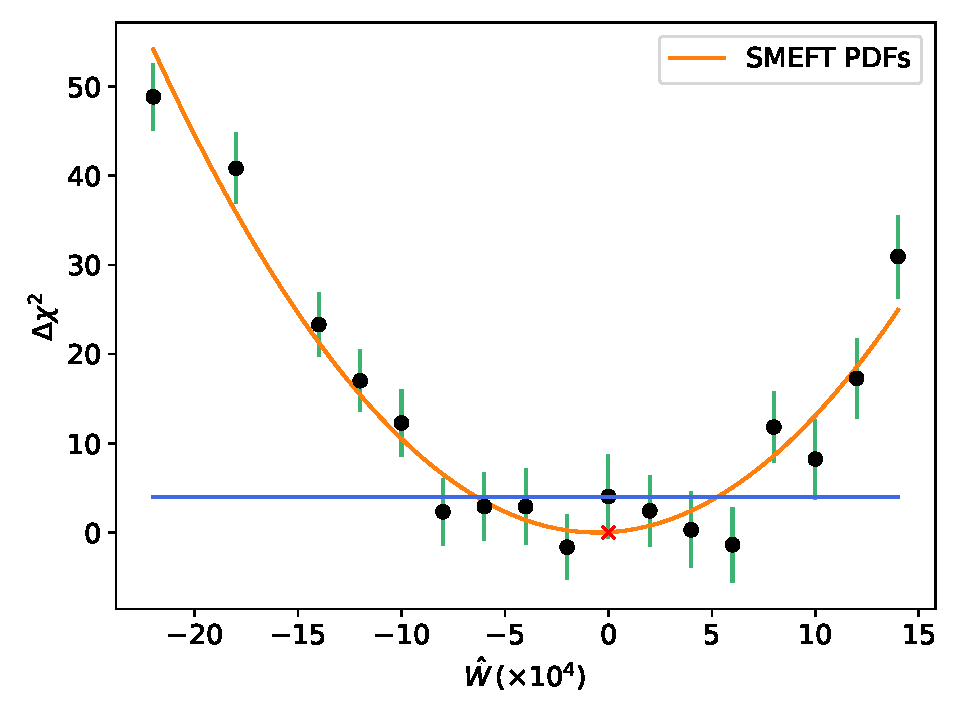
\includegraphics[width=0.49\textwidth]{dy_figures/W-smeftpdfs.pdf}
  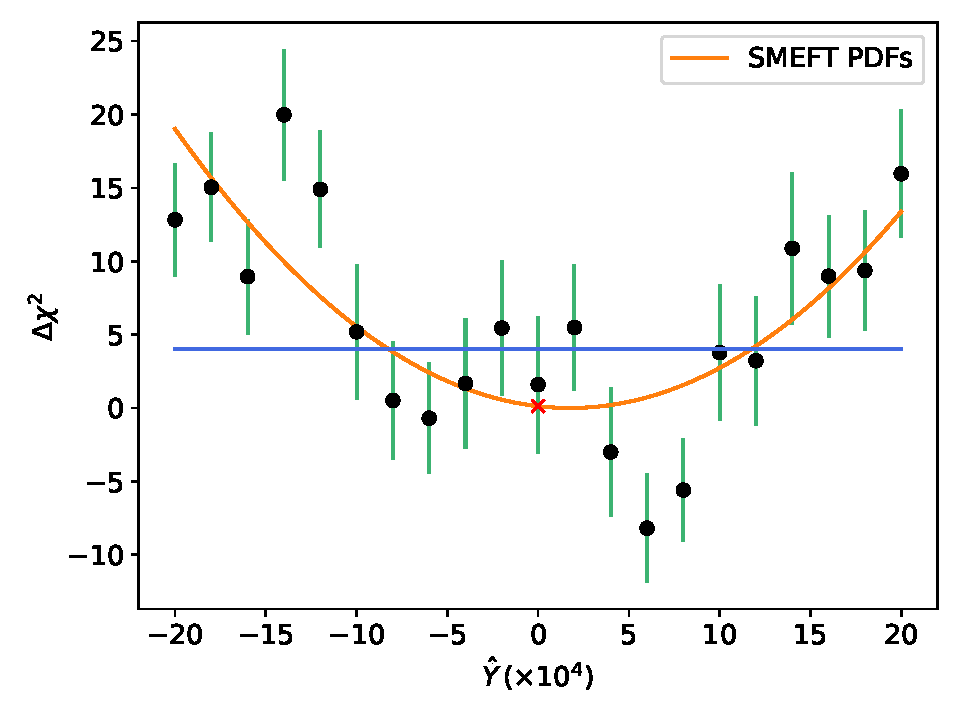
\includegraphics[width=0.49\textwidth]{dy_figures/Y-smeftpdfs.pdf}
    \caption{\label{fig:parabolas1} The values of $\Delta \chi^2$,
      Eq.~(\ref{eq:deltachi2def}), obtained for the SMEFT PDFs (thus using the
      $\chi_{\rm eftp}^2({\mathbf{c}_i})$ values)
  as a function of $\hat{W}$ (left)
      and $\hat{Y}$ (right panel) in the sampling ranges of
      Eq.~(\ref{eq:samplingrange})
      together with the corresponding parabolic fits.
      %
      The error bars indicate the finite-size
      uncertainties and the horizontal line corresponds to the $\Delta \chi^2=4$ condition
      defining the 95\% CL intervals.
      %
      The red cross indicates the SM expectation, $\hat{W}=\hat{Y}=0$.
      }
\end{center}
\end{figure}
%%%%%%%%%%%%%%%%%%%%%%%%%%%%%%%%%%%%%%%%%%%%%%%%%%%%%%%%%%%%%%%%%%%%%%%%%%%%%%%%%%

Fig.~\ref{fig:parabolas2} then compares the results
of the parabolic fits based on the SMEFT PDFs
as displayed in Fig.~\ref{fig:parabolas1} with their
counterparts
obtained in the case of the SM PDFs.
%
That is, in the latter case one carries out parabolic fits to
the $\chi^2_{{\rm smp}}$ values, as is customary
in the literature for the EFT analyses.
%
The insets highlight the region close to $\Delta\chi^2\simeq 0$.
%
For the $\hat{W}$ parameter, the consistent use of SMEFT PDFs leaves
the best-fit value essentially unchanged but increases the coefficient
uncertainty $\delta \hat{W}$, leading to a
broader parabola.
%
Similar observations can be derived for the $\hat{Y}$ parameter, though here
one also finds a upwards shift in the best-fit values by $\Delta\hat{Y}\simeq 2\times 10^{-4}$
in addition to a parabola broadening, when SMEFT PDFs are
consistently used.
%
We note that the SM PDF parabolas in Fig.~\ref{fig:parabolas2} are evaluated
using the central PDF replica and hence do not account for PDF uncertainties.

%%%%%%%%%%%%%%%%%%%%%%%%%%%%%%%%%%%%%%%%%%%%%%%%%%%%%%%%%%%%%%%%%%%%%%%%%%%%%%%%%%
\begin{figure}[t]
\begin{center}
  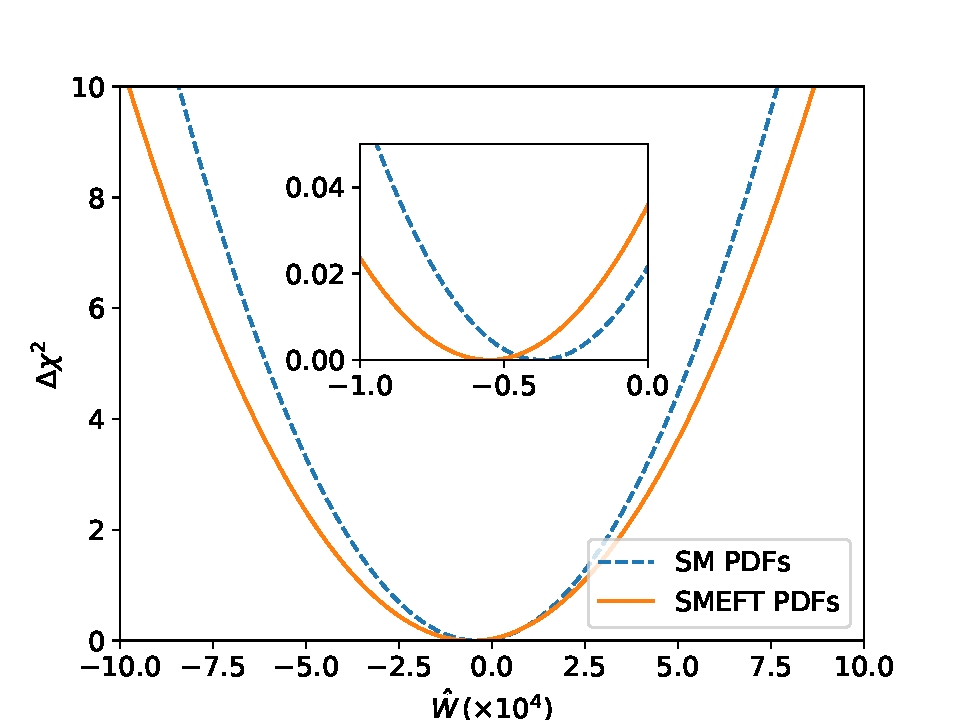
\includegraphics[width=0.49\textwidth]{dy_figures/W-both-parabs.pdf}
    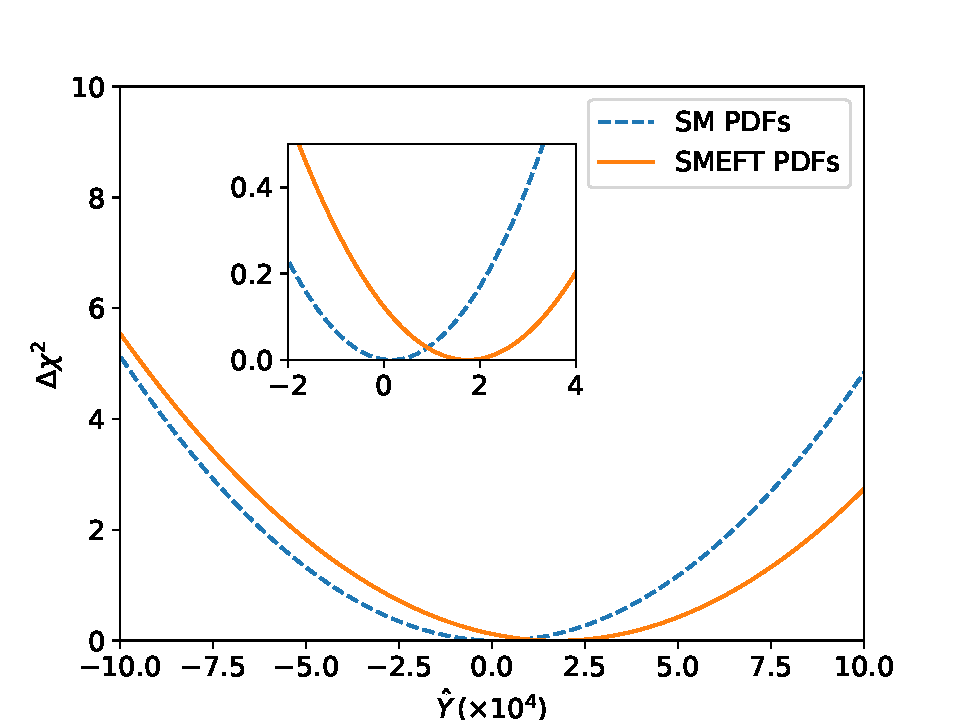
\includegraphics[width=0.49\textwidth]{dy_figures/Y-both-parabs.pdf}
    \caption{\label{fig:parabolas2} Comparison
      between the results of the parabolic fits to $\Delta\chi^2$, Eq.~(\ref{eq:parabolicfit}),
      for the $\hat{W}$ (left) and $\hat{Y}$ (right panel) parameters for either the SMEFT PDFs
      ($\chi^2_{\rm eftp}$, already displayed in Fig.~\ref{fig:parabolas1}) or
      the SM PDFs (hence with $\chi^2_{\rm smp}$).
      %
      The insets zoom on the region close to $\Delta\chi^2\simeq 0$.
    }
\end{center}
\end{figure}
%%%%%%%%%%%%%%%%%%%%%%%%%%%%%%%%%%%%%%%%%%%%%%%%%%%%%%%%%%%%%%%%%%%%%%%%%%%%%%%%%%

Table~\ref{tab:bound1w} summarises
the 68\% and 95\% CL bounds on the $\hat{W}$ and $\hat{Y}$
parameters obtained from the corresponding parabolic $\Delta\chi^2$ fits 
using either the SM or the SMEFT PDFs shown in Fig.~\ref{fig:parabolas2}.
%
The fourth and fifth column indicate the absolute shift in best-fit values
and the percentage broadening of the fit parameter uncertainties when the SMEFT PDFs
are consistently used instead of the SM PDFs (either without or with PDF uncertainties):
\begin{equation}
\label{eq:shift}
{\rm best~fit~shift}\equiv \left( \hat{W}^{(0)}\Big|_{\rm SMEFT\,PDF}-\hat{W}^{(0)}\Big|_{\rm SM\,PDF}\right) \, ,
\end{equation}
\begin{equation}
\label{eq:broadening}
{\rm broadening}\equiv \left( \delta\hat{W}^{(0)}\Big|_{\rm SMEFT\,PDF}-\delta\hat{W}^{(0)}\Big|_{\rm SM\,PDF}\right)\bigg/\delta\hat{W}^{(0)}\Big|_{\rm SM\,PDF} \, ,
\end{equation}
and likewise for the $\hat{Y}$ parameter.

%%%%%%%%%%%%%%%%%%%%%%%%%%%%%%%%%%%%%%%%%%%%%%%%%%%%%%%%%%%%%%%%%%%%%%%%%%%%%%%%%%
\begin{table}[t]
  \renewcommand{\arraystretch}{1.40}
  \centering
  \begin{tabular}{l|c|c|c|c}
    & $\quad$ SM PDFs $\quad$  & SMEFT PDFs  & best-fit shift  & broadening  \\
    \toprule
    \multirow{2}{*}{$\hat{W}\times 10^4$ (68\% CL)} & $[-3.0, 2.2] $ & \multirow{2}{*}{$[-3.5, 2.4]$}  & $-0.2$    &+13\%\\
    & $[-4.3, 3.8] $ &   &  $-0.3$   & $-27\%$ \\
    \midrule
    \multirow{2}{*}{$\hat{W}\times 10^4$ (95\% CL)} & $[-5.5, 4.7] $ &  \multirow{2}{*}{ $[-6.4, 5.3] $} & $-0.2$  & +15\%\\
     &   $[-6.8, 6.3] $   &  & $-0.3$      &$-11\%$ \\
    \midrule
    \multirow{2}{*}{$\hat{Y}\times 10^4$ (68\% CL)} & $[-4.4, 4.7] $ &  \multirow{2}{*}{$[-3.4, 6.9]$} & $+1.6$ &  $+13\%$\\
       & $[-6.7, 7.5] $ &   & $+1.4$ & $-27\%$ \\
    \midrule
    \multirow{2}{*}{$\hat{Y}\times 10^4$ (95\% CL)} & $[-8.8, 9.2] $ &  \multirow{2}{*}{$[-8.3, 11.8]$} & $+1.6$ & +12\% \\
     & $[-11.1, 12.0] $ &   & $+1.3$ & $-13\%$ \\
    \bottomrule
  \end{tabular}
  \caption{\label{tab:bound1w} \small The 68\% CL and 95\% CL bounds on the $\hat{W}$ and $\hat{Y}$
    parameters obtained from the  corresponding parabolic fits to
    the $\Delta\chi^2$ values calculated from  either the SM or the the SMEFT PDFs.
    %
    For the SM PDF results, we indicate the bounds obtained without (upper)
    and with (lower entry) PDF uncertainties accounted for; the SMEFT PDF
    bounds already include  PDF uncertainties by construction, while
    the methodological uncertainty is included according to the
    approached described in Sect.~3.4. 
    %
    The fourth and fifth column indicate the absolute shift in best-fit values,
    Eq.~(\ref{eq:shift})
    and the percentage broadening of the EFT parameter uncertainties, Eq.~(\ref{eq:broadening}),
    when the SMEFT PDFs
    are consistently used instead of the SM PDFs.
}
\end{table}
%%%%%%%%%%%%%%%%%%%%%%%%%%%%%%%%%%%%%%%%%%%%%%%%%%%%%%%%%%%%%%%%%%%%%%%%%%%]

In the specific case of the SM PDF results,
Table~\ref{tab:bound1w} indicates
the bounds obtained without (upper) and with (lower entry) PDF uncertainties accounted for;
recall that the SMEFT PDF bounds already include PDF uncertainties by construction
(see Sect.~\ref{eq:jointfits}).
By comparing the bounds obtained when PDF uncertainties are accounted for to
those neglecting PDF uncertainty, one observes a systematic broadening of the
bounds from both the lower and upper limits, as was also reported in~\cite{Carrazza:2019sec}.

When PDF uncertainties are neglected (accounted for) when using the SM PDFs
to constrain the EFT parameters,
 the consistent use of the SMEFT PDFs leads to both a shift
in the best-fit values of magnitude $\Delta\hat{W}=-2\times 10^{-5}$
and $\Delta\hat{Y}=+1.6\times 10^{-4}$ 
as well as to an increase (decrease) of the fit parameter uncertainties, with $\delta \hat{W}$
and $\delta \hat{Y}$ growing by 15\% and 12\% (decreasing by
11\% and  13\%) respectively.
%
This result shows that, given available Drell-Yan data and once PDF uncertainties
are accounted for, the bounds on the EFT parameters are actually {\it improved}
once SMEFT PDFs are adopted.

All in all, the effect of the consistent treatment of the SMEFT PDFs
in the interpretation of high-mass DY cross sections
is moderate but not negligible, either loosening or tightening up the obtained
bounds on the EFT parameters (depending on whether or not PDF uncertainties
are accounted for to begin with) by up to 15\% and, in the case of
$\hat{Y}$ parameter, shifting its central value by  one-third
of the 68\% CL parameter uncertainty.
%
Such a relatively moderate effect can be partly understood from the limited availability
of high-mass DY measurements for
EFT interpretations, with a single dataset at 13 TeV, and even in this case, with it being restricted to
a small fraction of the Run II luminosity.
%
As we will demonstrate in Sect.~\ref{sec:hllhc}, the impact of SMEFT
PDFs  becomes much more significant once higher-statistics measurements of the NC and CC Drell-Yan tails
become available at the HL-LHC, loosening the bounds on $\hat{W}$ and $\hat{Y}$
by up to a factor 5.

We now move to assess how the SMEFT PDFs relate to their SM counterparts,
and determine the extent to which it is possible to reabsorb EFT effects into the PDFs.
%
Fig.~\ref{fig:SMEFT_lumis} displays a
comparison between the SM and the SMEFT PDF luminosities 
for representative values of the $\hat{W}$ (upper) and $\hat{Y}$ (lower panel) parameters.
  %
  The values of $\hat{W}$ and $\hat{Y}$ are chosen to be close 
  to the upper and lower limits of the 95\% CL intervals reported in Table~\ref{tab:bound1w}.
  %
  The error band in the SM PDFs corresponds to the 68\% CL PDF uncertainty, while for the SMEFT
  PDFs only the central values are shown.

In all cases, one finds that the EFT-induced shifts on the luminosities are smaller
than their standard deviation.
%
The biggest differences, relative to uncertainties, are observed in the
quark-antiquark luminosities for $m_X \gsim$ 500 GeV.
This finding can be understood from the fact that the NC Drell-Yan cross section
is proportional to the $u\bar{u}$ and $d\bar{d}$ combinations at leading order,
but the up and down quark PDFs are already well constrained by lower-energy DIS measurements.
%
Furthermore, we have verified
that the size of the PDF uncertainties is unchanged in the SMEFT fits.
 %
The results of  Fig.~\ref{fig:SMEFT_lumis} are consistent with those of 
Table~\ref{tab:bound1w} and demonstrate
that, with current data, the interplay between EFT effects and 
PDFs in the high-mass Drell-Yan tails
is appreciable but remains subdominant as compared to other sources of uncertainty.

%%%%%%%%%%%%%%%%%%%%%%%%%%%%%%%%%%%%%%%%%%%%%%%%%%%%%%%%%%%%%%%%%%%%%%%%
\begin{figure}[t]
\begin{center}
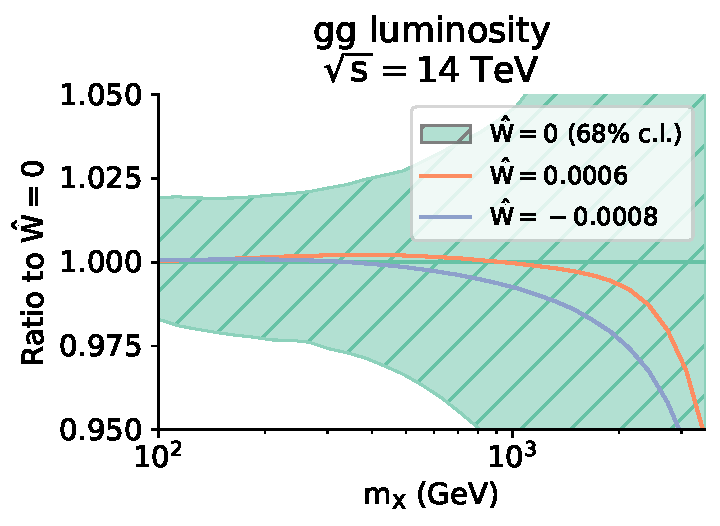
\includegraphics[width=0.32\textwidth]{dy_figures/SMEFTCoef_W_lumi_channels0_plot_lumi1d.pdf}
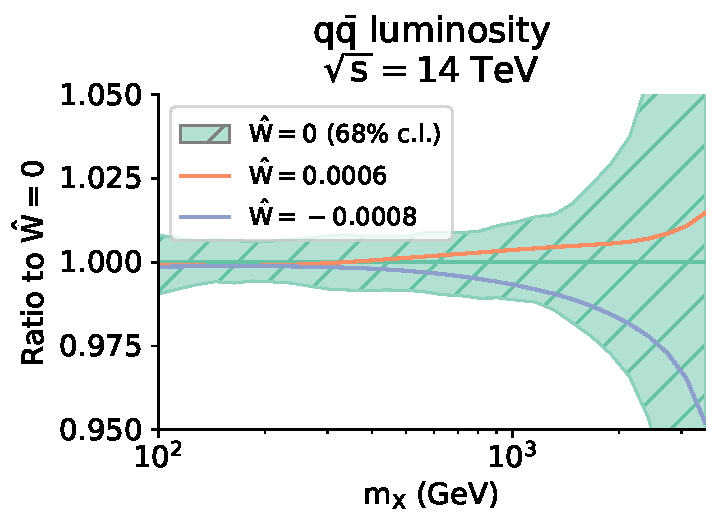
\includegraphics[width=0.32\textwidth]{dy_figures/SMEFTCoef_W_lumi_channels1_plot_lumi1d.pdf}
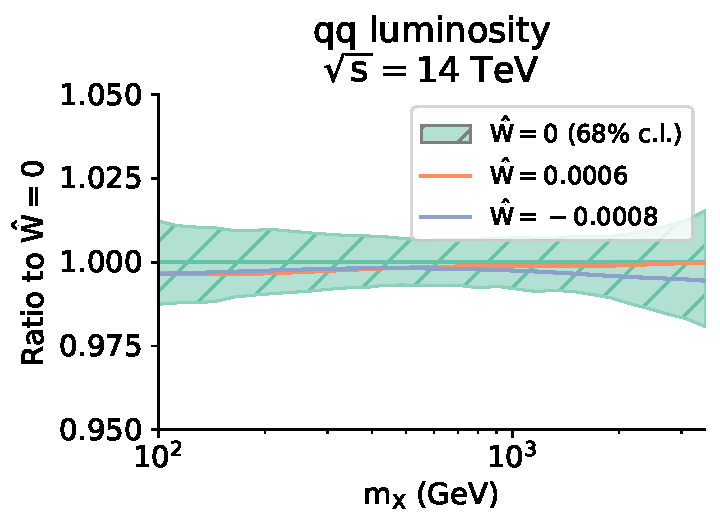
\includegraphics[width=0.32\textwidth]{dy_figures/SMEFTCoef_W_lumi_channels2_plot_lumi1d.pdf}
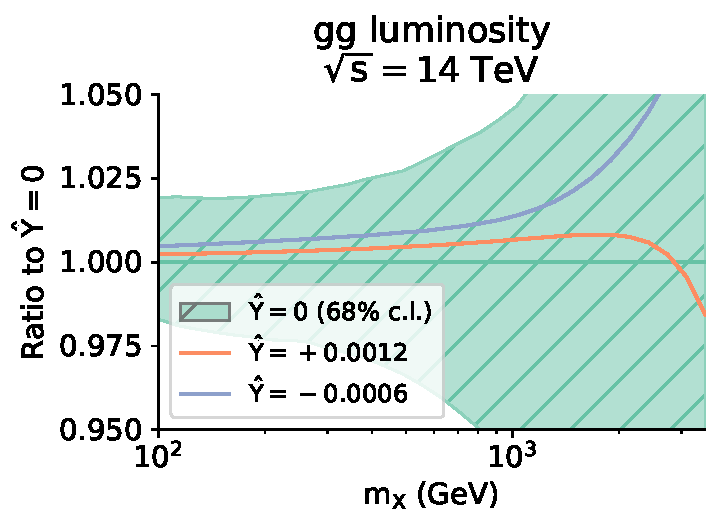
\includegraphics[width=0.32\textwidth]{dy_figures/SMEFTCoef_Y_lumi_channels0_plot_lumi1d.pdf}
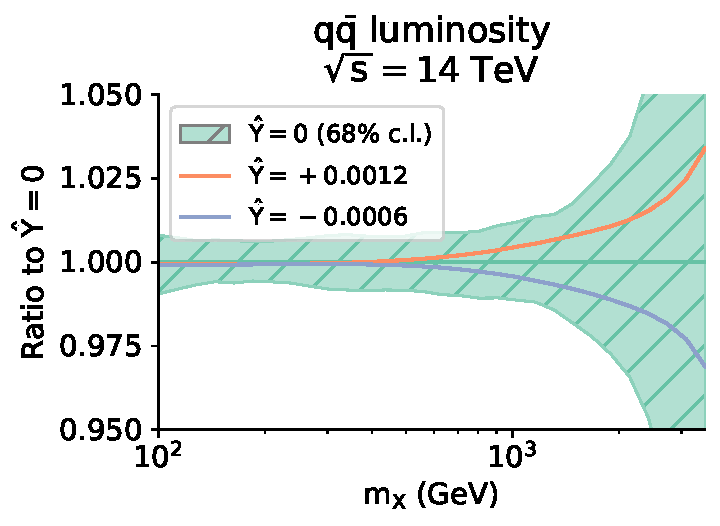
\includegraphics[width=0.32\textwidth]{dy_figures/SMEFTCoef_Y_lumi_channels1_plot_lumi1d.pdf}
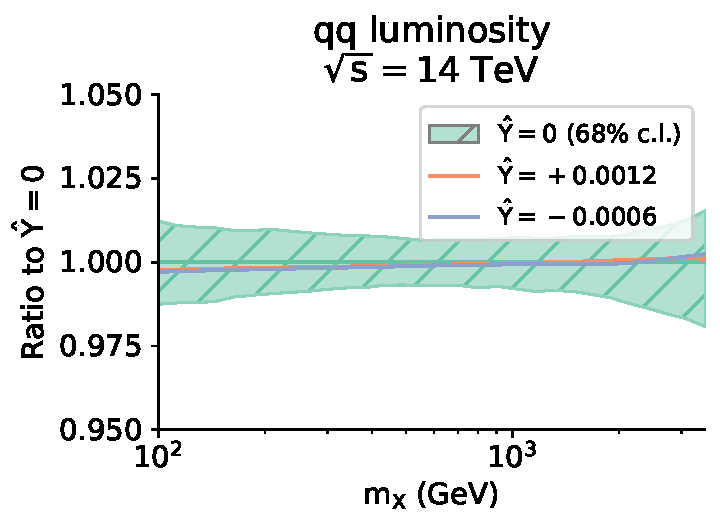
\includegraphics[width=0.32\textwidth]{dy_figures/SMEFTCoef_Y_lumi_channels2_plot_lumi1d.pdf}
\caption{\label{fig:SMEFT_lumis} 
Comparison between the SM PDF luminosities with their SMEFT counterparts, 
displayed as ratios to the central value of the SM luminosities, 
for representative values of the $\hat{W}$ (upper) and $\hat{Y}$ (lower panel)
parameters.
  %
  The values of $\hat{W}$ and $\hat{Y}$ are chosen to be close 
 to the upper and lower limits of the 95\% CL intervals reported in Table~\ref{tab:bound1w}.}
\end{center}
\end{figure}
%%%%%%%%%%%%%%%%%%%%%%%%%%%%%%%%%%%%%%%%%%%%%%%%%%%%%%%%%%%%%%%%%%%%%%%%

One important question in this context concerns how one could disentangle the EFT-induced shifts in
the PDF luminosities displayed in Fig.~\ref{fig:SMEFT_lumis} from other possible sources
of deviations, such as internal inconsistencies in some datasets or missing higher
orders in the SM calculations. A dedicated study to this end is performed in Chapter~\ref{chap:contamination}.

\section{Results from projected HL-LHC Drell-Yan data}
\label{sec:hllhc}
The results presented in the previous section indicate that,
given the available unfolded Drell-Yan measurements,
the impact of a  simultaneous determination of the PDFs together with the EFT parameters
remains moderate.
%
However, it is conceivable that this
interplay between PDFs and BSM effects in the high-energy tails of
Drell-Yan cross sections will become more significant once more data are accumulated.
%
With this motivation, we revisit the analysis of Sect.~\ref{sec:res1}
now accounting for the impact of projected High-Luminosity LHC pseudo-data generated for the present study.
%
We demonstrate that a consistent joint determination of PDFs is crucial for
EFT studies at the HL-LHC.

\subsection{Generation of HL-LHC pseudo-data}
The HL-LHC pseudodata in this chapter is generated in the same way as in Sect.~\ref{subsec:dark_constraints}
of Chapter~\ref{chap:darkphoton}. However, here we also generate data for charged-current DY data,
whereas in Sect.~\ref{subsec:dark_constraints} we used only neutral-current DY data.
Additionally, the PDF set used as an input to
generate the theoretical prediction on which the pseudodata is based
 is the DIS+DY baseline that was presented
in Sect.~\ref{sec:fitsettings} (rather than the \texttt{luxQED} set used in Sect.~\ref{subsec:dark_constraints}).

In the case of the  CC pseudo-data, the lack of unfolded measurements
of the $m_T$ distribution at 13 TeV to be used as reference forces
us to base our projections on the
ATLAS search for $W'$ bosons in the dilepton channel~\cite{Aad:2019wvl}.
%
As in the case of the NC projections (discussed in Sect.~\ref{subsec:dark_constraints}), theory predictions for
the $m_T$ distribution at high-mass are generated
using the same selection and acceptance cuts as in~\cite{Aad:2019wvl}
but now using an extended coverage in $m_T$. Further, we similarly restrict ourselves
to events with either $m_{\ell\ell}$ or $m_T$ greater than 500 GeV.

The pseudodata for the $m_{\ell\ell}$~($m_T$) distribution at the HL-LHC
is displayed in Fig.~\ref{fig:hllhc-nc}~(Fig.~\ref{fig:hllhc-cc}),
with the highest energy bins reaching $m_{\ell\ell}\simeq 4 $ TeV
($m_T\simeq 3.5$ TeV) for neutral-current (charged-current) scattering.

%%%%%%%%%%%%%%%%%%%%%%%%%%%%%%%%%%%%%%%%%%%%%%%%%%%%%%%%%%%%%%%%%%%%%%%%%%%%%%%%%%
\begin{figure}[t]
\begin{center}
  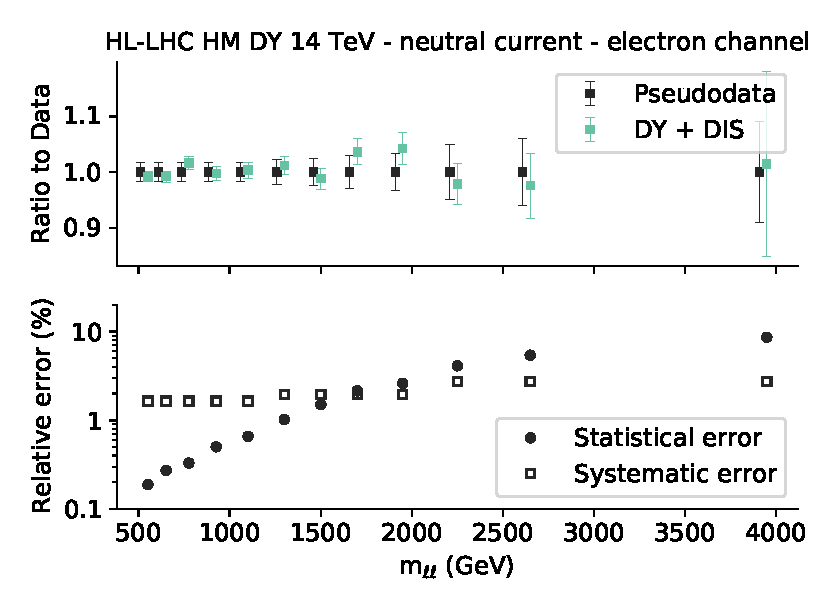
\includegraphics[width=0.49\textwidth]{dy_figures/HLLHC_HMDY_NC_EL_FINAL_plot_error_breakdown_0.pdf}
  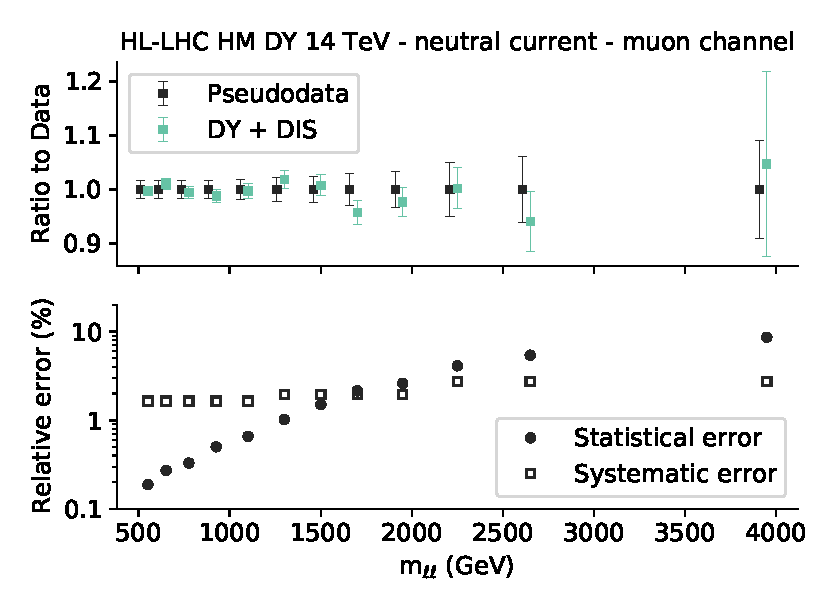
\includegraphics[width=0.49\textwidth]{dy_figures/HLLHC_HMDY_NC_MU_FINAL_plot_error_breakdown_0.pdf}
  \caption{\label{fig:hllhc-nc} Top panels: comparison  of the
    projected HL-LHC pseudo-data for high-mass neutral-current Drell-Yan in the dielectron (left)
    and dimuon (right) final states
    as a function of $m_{\ell\ell}$ with
    the corresponding theory predictions obtained from the SM PDF
    baseline. The theoretical predictions, generated according to
    Eq.~\eqref{eq:hllhc}, are accompanied by their corresponding PDF
    uncertainties (green bars). 
    %
    Lower panels: the percentage statistical and systematic uncertainty in each  $m_{\ell\ell}$ bin
    of the HL-LHC pseudo-data.
    }
\end{center}
\end{figure}
%%%%%%%%%%%%%%%%%%%%%%%%%%%%%%%%%%%%%%%%%%%%%%%%%%%%%%%%%%%%%%%%%%%%%%%%%%%%%%%%%%%%%%%%%%%%%


%%%%%%%%%%%%%%%%%%%%%%%%%%%%%%%%%%%%%%%%%%%%%%%%%%%%%%%%%%%%%%%%%%%%%%%%%%%%%%%%%%
\begin{figure}[t]
\begin{center}
  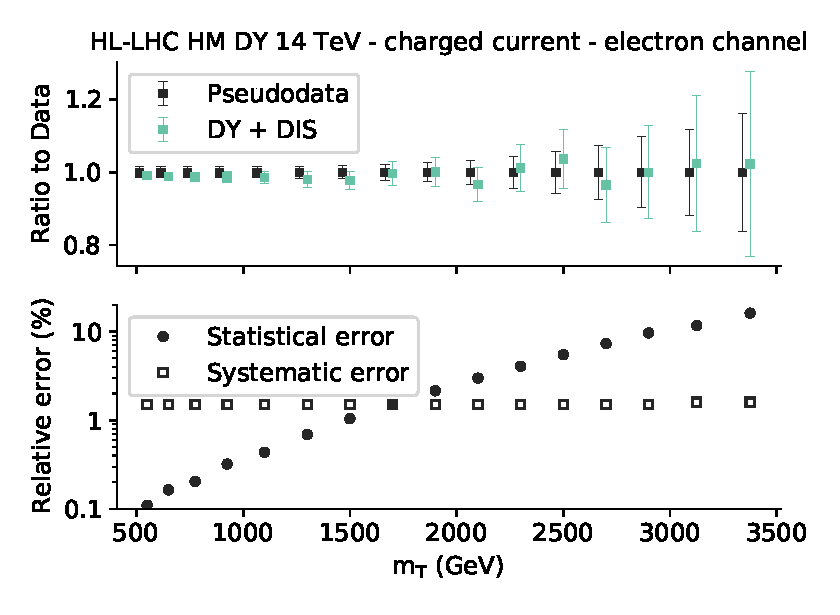
\includegraphics[width=0.49\textwidth]{dy_figures/HLLHC_HMDY_CC_EL_FINAL_plot_error_breakdown_0.pdf}
  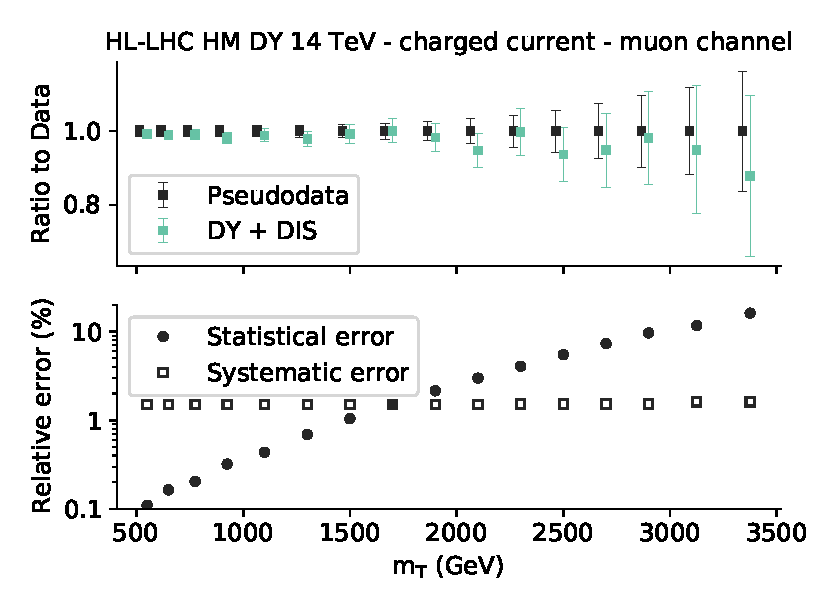
\includegraphics[width=0.49\textwidth]{dy_figures/HLLHC_HMDY_CC_MU_FINAL_plot_error_breakdown_0.pdf}
    \caption{\label{fig:hllhc-cc} Same as Fig.~\ref{fig:hllhc-nc} for
      charged-current Drell-Yan in bins of the transverse mass $m_T$.
    }
\end{center}
\end{figure}
%%%%%%%%%%%%%%%%%%%%%%%%%%%%%%%%%%%%%%%%%%%%%%%%%%%%%%%%%%%%%%%%%%%%%%%%%%%%%%%%%%

The percentage statistical and systematic uncertainties associated to the HL-LHC pseudo-data
are displayed in the lower panels of Figs.~\ref{fig:hllhc-nc} and~\ref{fig:hllhc-cc}, and are 
estimated using the same procedure as outlined in Sect.~\ref{subsec:dark_constraints} (choosing
to work with a five-fold reduction factor for the systematics, corresponding to the \textit{optimistic} 
scenario there\footnote{We note that the \textit{conservative scenario} for the reduction of systematic errors,
namely $f_{{\rm red},j}=0.5$, is not expected to qualitatively
modify our results.
%
The reason is that, as indicated by
the bottom panels of Figs.~\ref{fig:hllhc-nc} and~\ref{fig:hllhc-cc},
for the highest energy bins (which dominate
the EFT sensitivity), specifically above
$m_{\ell\ell}\approx$ 1.7 TeV and $m_T \approx$ 1.5 TeV, the measurement
will be limited by statistical uncertainties.}). As in Sect.~\ref{subsec:dark_constraints}, the central values for the HL-LHC pseudodata are then generated
by fluctuating the reference theory prediction by the expected total experimental
uncertainty, namely:
\begin{equation}
  \label{eq:hllhc}
\sigma^{\rm hllhc}_{i} \equiv \sigma^{\rm th}_{i} \left( 1+ \lambda
  \delta_{\cal L}^{\rm exp} +  r_i\delta_{{\rm tot},i}^{\rm exp}   \right) \, , \qquad i=1,\ldots,n_{\rm bin} \, ,
\end{equation}
where $\lambda,r_i$ are univariate Gaussian random numbers, $\delta_{{\rm tot},i}^{\rm exp}$
is the total (relative) experimental uncertainty corresponding to this
specific bin
(excluding the luminosity and normalisation uncertainties), and $\delta_{\cal L}^{\rm exp}$
is the luminosity uncertainty, which is fully correlated amongst all
the pseudo-data bins of the same experiment. Again, we take this luminosity uncertainty to be
$\delta_{\cal L}^{\rm exp}=1.5$\%  for both ATLAS and CMS, as done in Ref.~\cite{Khalek:2018mdn}.

We have verified that, both at the pre- and post-fit levels, the fit quality to the HL-LHC pseudo-data
satisfies $\chi^2/n_{\rm bin} \simeq 1$ in the case of the SM PDFs
as expected.


\subsection{Impact on PDF uncertainties}

From Figs.~\ref{fig:hllhc-nc} and \ref{fig:hllhc-cc},  one can observe that
the PDF uncertainties in the SM PDF baseline used to generate the pseudodata
are either comparable or larger than the corresponding
projected experimental uncertainties at the  HL-LHC.
%
Specifically, for the highest $m_{\ell\ell}$ bin
of the NC distribution the PDF errors are twice the experimental ones,
while in the CC case the associated PDF errors become clearly larger
than the experimental ones starting at $m_T\simeq 2 $ TeV.
%
This comparison suggests that one should expect a significant 
uncertainty reduction once the HL-LHC pseudodata is included
in the PDF fit.

%%%%%%%%%%%%%%%%%%%%%%%%%%%%%%%%%%%%%%%%%%%%%%%%%%%%%%%%%%%%%%%%%%%%%%%%%
\begin{figure}[t]
\begin{center}
  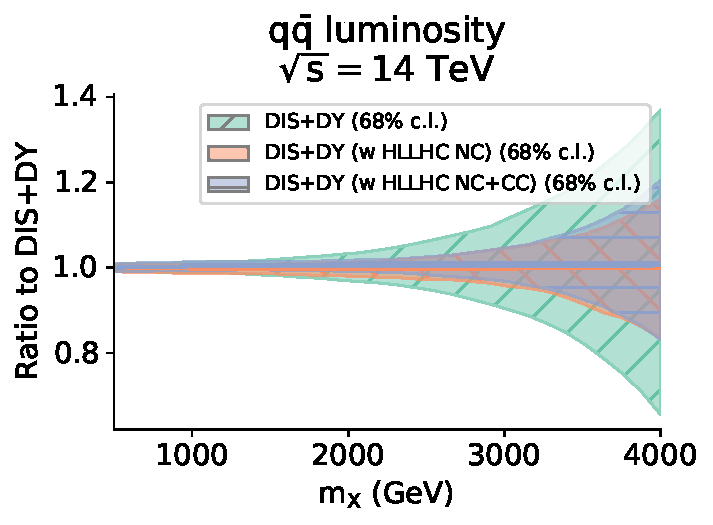
\includegraphics[width=0.49\textwidth]{dy_figures/DataHL_lumi_channels0_plot_lumi1d.pdf}
  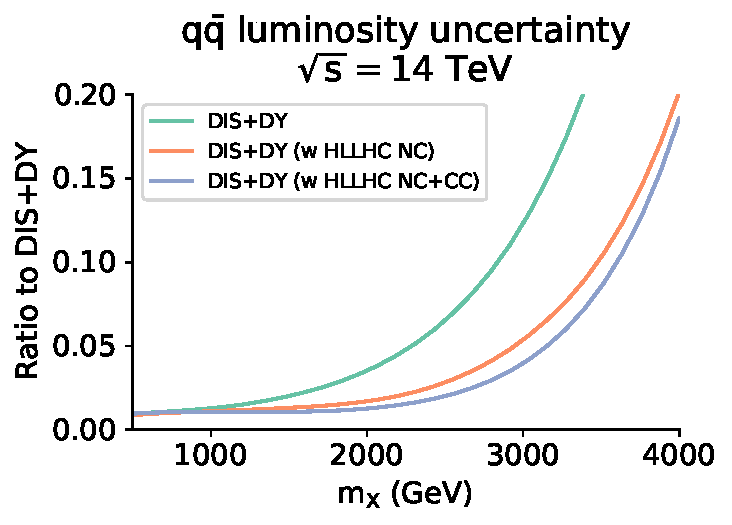
\includegraphics[width=0.49\textwidth]{dy_figures/DataHL_lumi_channels0_UncRange_plot_lumi1d_uncertainties.pdf}
    \caption{\label{fig:hllhc-lumi-qqb} Impact of the
      HL-LHC pseudo-data on the quark-antiquark luminosity $\mathcal{L}_{q\bar{q}}$
      of the SM PDF baseline fit as a function
      of  $m_X$.
      %
      Left: the luminosities $\mathcal{L}_{q\bar{q}}$ for the DIS+DY baseline
      and the corresponding fits including the HL-LHC pseudo-data, either only NC
      or also with CC cross sections, presented as a ratio to the central value of the former.
      %
      Right: the relative PDF uncertainty in $\mathcal{L}_{q\bar{q}}$ (with the central
      value of the DIS+DY baseline as reference) for the same fits.
    }
\end{center}
\end{figure}
%%%%%%%%%%%%%%%%%%%%%%%%%%%%%%%%%%%%%%%%%%%%%%%%%%%%%%%%%%%%%%%%%%%%%%%%%

To validate this expectation, Fig.~\ref{fig:hllhc-lumi-qqb} displays
the impact of the
HL-LHC pseudo-data on the quark-antiquark luminosity $\mathcal{L}_{q\bar{q}}$
as a function
of the final state invariant mass $m_X$ at $\sqrt{s}=14$ TeV.
%
We compare  $\mathcal{L}_{q\bar{q}}$ for the SM PDF baseline fit (DIS+DY)
with the same quantity from the corresponding fits including the HL-LHC pseudo-data, either only NC
or also with CC cross sections.
%
The right panel displays the associated relative PDF uncertainties.
We find a significant reduction of the PDF uncertainties
affecting the quark-antiquark luminosity (and hence the Drell-Yan
cross sections) in the high mass ($m_X\gsim$ 1 TeV) region
once the HL-LHC pseudo-data constraints are accounted for.
%
For instance, at  $m_X\gsim$ 2 TeV, PDF uncertainties on $\mathcal{L}_{q\bar{q}}$
decrease from $\simeq5\%$ in the baseline down to $\simeq 2.5\%$~($\simeq 1.5\%$)
once the NC~(NC+CC) HL-LHC pseudo-data is included in the fit. The
effect of the inclusion of HL-LHC projections becomes more dramatic as
$m_X$ increases. 
%
On the other hand, other partonic luminosities such as the quark-quark
and gluon-gluon ones are essentially unaffected by the HL-LHC constraints.
%
In terms of fit quality, the only noticeable effect is a mild
improvement in the $\chi^2$ of the high-mass DY datasets listed in
Table~\ref{tab:data-high-mass}. 

%%%%%%%%%%%%%%%%%%%%%%%%%%%%%%%%%
\subsection{PDF and EFT interplay at the HL-LHC}
\label{sec:hllhc_joint_fits}
%%%%%%%%%%%%%%%%%%%%%%%%%%%%%%%%%

The finding  that the projected HL-LHC pseudo-data has a significant
impact on the quark-antiquark PDF luminosity, summarised in  Fig.~\ref{fig:hllhc-lumi-qqb}, 
 suggests that
the interplay between PDFs and EFT effects in the high-energy
DY tails should become enhanced
as compared to the results reported in the previous section.
%
With this motivation, we first of all repeat the joint
determination of PDFs and the $\hat{W},\hat{Y}$ coefficients
from the benchmark scenario presented in Sect.~\ref{sec:res1}
now accounting for the constraints of the HL-LHC pseudo-data.
%
An important difference in this case is that the
inclusion of CC data lifts the flat direction in the $(\hat{W},\hat{Y})$
plane, making a full two-dimensional fit possible.\\

\noindent For the simultaneous determination of PDFs and the $\hat{W},\hat{Y}$ coefficients
accounting for the constraints provided by the HL-LHC pseudo-data,
we use 35 sampling values of $(\hat{W},\hat{Y})$, 25 of which are equally spaced in
either $\hat{W}\in (-1.6,1.6)\times 10^{-5}$ or $\hat{Y}\in (-8,+8)\times 10^{-5}$
(hence in steps of $\Delta\hat{W}=0.8 \times 10^{-6}$ and
$\Delta\hat{Y}=4 \times 10^{-6}$ respectively), and then 10 additional points along the
diagonals.
%
In order to assess the robustness of the results, we added 12
more sampling values, 8 further away from the origin and 4 more along
the $\hat{W}=0$ and $\hat{Y}=0$ axes, and verified that the confidence
level contours are stable upon their addition. 

We find that the constraints on the $(\hat{W},\hat{Y})$ parameters are completely
dominated by the HL-LHC projections and that current data exhibit a much
smaller pull, consistent with the findings of previous
studies~\cite{Farina:2016rws,Ricci:2020xre}. Also, the $\chi^2_{\rm
  eftp}$ contour is more stable and requires less replicas if only the HL-LHC projections
are included in the computation of the $\chi^2$.
%
The corresponding 
marginalised bounds on $\hat{W}$ and $\hat{Y}$
are reported in Table~\ref{tab:hlbounds} using the same
format as in  Table~\ref{tab:bound1w}.

%%%%%%%%%%%%%%%%%%%%%%%%%%%%%%%%%%%%%%%%%%%%%%%%%%%%%%%
\begin{table}
 \renewcommand{\arraystretch}{1.40}
  \centering
  \begin{tabular}{l|c|c|c|c}
    & SM PDFs & SMEFT PDFs  & best-fit shift  & broadening  \\
    \hline
    \multirow{2}{*}{ $\hat{W}\times 10^5$ (68\% CL)} & $[-0.7, 0.5]$ & \multirow{2}{*}{$[-4.5, 6.9]$}  & 1.3 & 850\% \\
      & $[-1.0, 0.9]$ &  & 1.3  & 500\% \\
    \midrule
    \multirow{2}{*}{$\hat{W}\times 10^5$ (95\% CL)} & $[-1.0, 0.8]$ & \multirow{2}{*}{$[-8.1, 10.6]$} & 1.4 & 940\%\\
      & $[-1.4, 1.2]$ &  &  1.4 & 620\%  \\
   \hline
   \multirow{2}{*}{$\hat{Y}\times 10^5$ (68\% CL)} & $[-1.8, 3.2]$ & \multirow{2}{*}{$[-6.4, 8.0]$} & 0.1 & 190\% \\
       & $[-3.7, 4.7] $ &  & 0.3  & 70\% \\
   \midrule
   \multirow{2}{*}{$\hat{Y}\times 10^5$ (95\% CL)} & $[-3.4, 4.7] $ & \multirow{2}{*}{$[-11.1, 12.6]$} & 0.1 & 190\%\\
   & $[-5.3, 6.3] $ &  & 0.3  & 110\% \\
    \hline
  \end{tabular}
  \caption{ \label{tab:hlbounds}\small
    Same as Table~\ref{tab:bound1w} for the
 68\% CL and 95\% CL
    marginalised bounds on the $\hat{W}$ and $\hat{Y}$
    parameters obtained from the two-dimensional ($\hat{W}$,$\hat{Y}$)
    fits that include the HL-LHC pseudo-data for NC and CC
    Drell-Yan distributions.
    %
    As in Table~\ref{tab:bound1w},
    for the SM PDFs we indicate the bounds obtained without (upper)
    and with (lower entry) PDF uncertainties accounted for.
}
\end{table}
%%%%%%%%%%%%%%%%%%%%%%%%%%%%%%%%%%%%%%%%%%%%%%%%%%%%%%%

From Table~\ref{tab:hlbounds},
one can observe how including high-mass data at the LHC both in a fit of PDFs and
in a fit of SMEFT coefficients and neglecting the interplay between
them could result in a significant underestimate
of the uncertainties associated to the EFT parameters.
%
Indeed, the marginalised 95\% CL bound on the $\hat{W}$~($\hat{Y}$) parameter becomes looser
once SMEFT PDFs are consistently used, with a broadening, defined in Eq.~(\ref{eq:broadening}),
of 500\%~(110\%), even once PDF uncertainties are fully accounted for. 
%
This effect would have been even more marked if PDF uncertainties had not
been accounted for in EFT fits based on SM PDFs,
where the same broadening factors would be 940\% and 190\%
respectively.

%
%%%%%%%%%%%%%%%%%%%%%%%%%%%%%%%%%%%%%%%%%%%%%%%%%%%%%%%
\begin{table}
 \renewcommand{\arraystretch}{1.40}
  \centering
  \begin{tabular}{l|c|c|c|c}
    & SM cons. PDFs & SMEFT PDFs  & best-fit shift  & broadening  \\
    \hline
    \multirow{2}{*}{ $\hat{W}\times 10^5$ (68\% CL)} & $[-1.0, 0.0]$ & \multirow{2}{*}{$[-4.5, 6.9]$}  & 1.7 & 1000\% \\
                                                                        & $[-4.0, 2.8]$ &  & 1.8  & 70\% \\
    \midrule
    \multirow{2}{*}{$\hat{W}\times 10^5$ (95\% CL)} & $[-1.4, 0.4]$ & \multirow{2}{*}{$[-8.1, 10.6]$} & 1.8 & 940\%\\
    & $[-4.3, 3.1]$ &  &  1.9 & 150\%  \\
    \hline
   \multirow{2}{*}{$\hat{Y}\times 10^5$ (68\% CL)} & $[2.1, 7.0]$ & \multirow{2}{*}{$[-6.4, 8.0]$} & -3.7 & 190\% \\
       & $[-3.4,11.2] $ &  & -3.6  & -1\% \\
   \midrule
   \multirow{2}{*}{$\hat{Y}\times 10^5$ (95\% CL)} & $[0.5, 8.5] $ & \multirow{2}{*}{$[-11.1, 12.6]$} & -3.7 & 200\%\\
   & $[-5.0, 13.7] $ &  & -3.6  & 30\% \\
    \hline
  \end{tabular}
  \caption{ \label{tab:hlboundscons}\small
    Same as Table~\ref{tab:hlbounds} for the 68\% and 95\% CL
    marginalised bounds on the $\hat{W}$ and $\hat{Y}$
    parameters obtained from the two-dimensional ($\hat{W}$,$\hat{Y}$)
    fits that include the HL-LHC pseudo-data for NC and CC
    Drell-Yan distributions. The input PDF set for the analysis done
    using fixed SM PDFs (corresponding to the results displayed in the
    column `SM cons. PDFs') is a conservative PDF set that does not
    include any of the high-mass
    distributions or the HL-LHC projections nor the Run I and
    Run II high-mass dataset listed in Table
    ~\ref{tab:data-high-mass}. The limits obtained from the simultaneous fit
    of PDFs and Wilson coefficients  (corresponding to the results displayed on the
    column `SMEFT PDFs') are the same as those in Table~\ref{tab:hlbounds}. 
}
\end{table}
%%%%%%%%%%%%%%%%%%%%%%%%%%%%%%%%%%%%%%%%%%%%%%%%%%%%%%%
%

A further important question is whether the bounds obtained with SM
PDFs appearing on the left column of Table~\ref{tab:hlbounds}  would become
more comparable to those obtained from the simultaneous fit of PDFs
and SMEFT coefficients, in case a
conservative set of PDF was used in the analysis based on SM PDFs. To
address this question, in Table~\ref{tab:hlboundscons} we display the
bounds that are obtained using a PDF set that does not include any of
the high-mass Drell-Yan sets (neither the HL-LHC projections nor the
current datasets listed in Table.~\ref{tab:data-high-mass}) and
compare the bounds obtained using this set of PDFs to those obtained
consistently using SMEFT PDFs.
%
We observe that, once this set of conservative PDF is used as an input
PDF set and the PDF uncertainty is included in the computation of the
bounds, the latter increases as compared to the bounds in
Table~\ref{tab:hlbounds}. As a result, the size of the bounds obtained
by keeping fixed SM PDFs is closer to the size obtained from the
simultaneous fits, although still slightly underestimated.
At the same time, the shift in the best-fit becomes more
marked.


%%%%%%%%%%%%%%%%%%%%%%%%%%%%%%%%%%%%%%%%%%%%%%%%
\begin{figure}[t]
\begin{center}
  \includegraphics[width=0.9\textwidth]{dy_figures/WY-contours-sm-smeft-hl-ref-160621-2.pdf}
  \caption{\label{fig:hllhc-ellipse} The 95\% confidence level contours
    in the ($\hat{W}$,$\hat{Y}$) plane obtained from the DIS+DY fits that
    include the high-mass Drell-Yan HL-LHC pseudo-data (both in the NC
    and CC channels) 
    when using either SM PDFs (blue) or conservative SM PDFs (green). In both cases
    the ellipses are obtained by performing a parabolic fit to
    $\chi^2_{\rm smp}$ with fixed PDFs. PDF
    uncertainties are included in the solid lines and not included in
    the dashed lines.  The results are compared to
    those obtained in a simultaneous fit, namely with SMEFT PDFs
    (orange). In this case, the parabolic fit is performed to $\chi^2_{\rm eftp}$ by varying
    simultaneously the Wilson Coefficients and the PDFs. 
    %
    The crosses indicate the best fits in the three cases discussed in
    the text. }
\end{center}
\end{figure}
%%%%%%%%%%%%%%%%%%%%%%%%%%%%%%%%%%%%%%%%%%%%5
Results are graphically displayed in
Fig.~\ref{fig:hllhc-ellipse}, where the 95\% confidence level contours
    in the ($\hat{W}$,$\hat{Y}$) plane obtained from the DIS+DY fits that
    include the high-mass Drell-Yan HL-LHC pseudo-data  when using either SM PDFs, SM conservative
    PDFs or SMEFT PDFs are compared. All solid contours include PDF
    uncertainties, while the dashed contours that do not include PDF
    uncertainties are also indicated to visualise the impact of the
    inclusion of the PDF uncertainties.

  To conclude, we should also emphasise that, while in this chapter we use pseudodata
and hence the best-fit values are by construction unchanged, this
would not necessarily be the case in the analysis of real data, where
improper treatment of PDFs could result in a spurious EFT `signal', or
even missing a signal which is indeed present in the data. A detailed
study aimed at a precise definition of `conservative' PDFs is given in Chapter~\ref{chap:contamination}; 
a thorough comparison of the consistent
simultaneous approach, versus the use of conservative PDF sets, will
be of particular interest in cases of EFT manifestations of new
physics.

The increased role that the interplay between PDFs and EFT coefficients
will play at the HL-LHC can also be illustrated by
comparing the expected behaviour of the quark-antiquark
luminosity, displayed in Fig.~\ref{fig:HLlumiWY},
for the SMEFT PDFs corresponding
to representative values of the $\hat{W}$ and $\hat{Y}$ parameters of the benchmark scenario
as compared to the  SM PDFs.
%
Note that the corresponding comparison for $\mathcal{L}_{q\bar{q}}$ 
in the fits to available Drell-Yan data
    was displayed in Fig.~\ref{fig:SMEFT_lumis}.
%
    Indeed, the central value of the quark-antiquark luminosity
    for SMEFT PDFs corresponding to values of $(\hat{W},\hat{Y})$ selected along the grid used
    to derive
Fig.~\ref{fig:HLlumiWY} changes greatly, well
outside the one-sigma error band of the SM PDFs, while the
PDF uncertainties themselves are unchanged. 
%
This change in central value of the large-$x$ PDFs partially reabsorbs the effects in the
partonic cross section induced by the SMEFT operators and leads to better
$\chi^2$ values as compared to those obtained with the SM PDFs.

%%%%%%%%%%%%%%%%%%%%%%%%%%%%%%%%%%%%%%%%%%%%%%%%%%%%%%%%%%%%%%%%%%%%5
\begin{figure}[t]
\begin{center}
  \includegraphics[width=0.49\textwidth]{dy_figures/HighLumiCoef_lumi_channels0_plot_lumi1d.pdf}
  \includegraphics[width=0.49\textwidth]{dy_figures/HighLumiCoef_lumi_channels0_UncRange_plot_lumi1d_uncertainties.pdf}
  \caption{\label{fig:HLlumiWY} Same as Fig.~\ref{fig:hllhc-lumi-qqb}, now comparing
    the quark-antiquark SM PDF luminosity in the fits including the HL-LHC pseudodata
    with those obtained in the SMEFT PDF fits for representative values
    of the $\hat{W}$ and $\hat{Y}$ parameters.
    %
    The corresponding comparison in the case of fits to available Drell-Yan data
    was shown in Fig.~\ref{fig:SMEFT_lumis}.
  }
\end{center}
\end{figure}
%%%%%%%%%%%%%%%%%%%%%%%%%%%%%%%%%%%%%%%%%%%%%%%%%%%%%%%%%%%%%%%%%%%%%%%%%%

Even neglecting SMEFT PDF effects, we note that our marginalised bounds on
the $\hat{W}$ and $\hat{Y}$ coefficients from HL-LHC pseudo-data using SM
PDFs turn out to be more stringent than those reported
in~\cite{Ricci:2020xre} by around a factor of 4 for $\hat{W}$ and a factor 2
for $(\hat{Y})$.
%
This is due to a combination of factors. First of all we use the 13
TeV measurements as reference to produce the HL
projections. Furthermore we assume a total integrated
luminosity of $\mathcal{L}=6$ fb$^{-1}$ (from the combination
of ATLAS and CMS) rather than 3 fb$^{-1}$ as well as a more optimistic
scenario concerning the reduction of the experimental systematic
uncertainties.



\section{A first look at PDF `contamination': injecting New Physics into the HL-LHC data}
\label{sec:hllhc_extension}

The study presented in Sect.~\ref{sec:hllhc} was based entirely on the assumption that data on NC and CC DY from the HL-LHC will be entirely consistent with the Standard Model. It is interesting to ask what happens if instead we inject the data with some New Physics, that is, if we base the generation of the HL-LHC pseudodata in Sect.~\ref{sec:hllhc} not on SM central values, but instead on SM central values multiplied by some non-unit $K$-factor combination of the $\hat{W}, \hat{Y}$ parameters. Such a study was performed in the conference proceedings given in Ref.~\cite{Madigan:2021uho}, and is described here.

Let us suppose that we now generate the HL-LHC pseudodata in Sect.~\ref{sec:hllhc} with $\hat{W},\hat{Y}$ fixed to the values $(\hat{W}, \hat{Y}) = (4,8) \times 10^{-5}$, taking these values from within the 95\% confidence intervals presented in Sect.~\ref{sec:hllhc}. Performing the same analysis, and in particular recomputing the EFT bounds, we obtain the results given in Table~\ref{tab:hllhc_w_y_bounds}.

\begin{table}[H]
 \renewcommand{\arraystretch}{1.40}
  \centering
  \begin{tabular}{l|c|c|c}
    & SM PDFs & SM cons. PDFs  & SMEFT PDFs \\
    \hline
    $\hat{W}\times 10^5$ (95\% CL)& $[-1.5,1.2]$ & $[3.1,5.0]$ & $[-5.3,9.0]$ \\
    \hline
   $\hat{Y}\times 10^5$ (95\% CL) & $[-3.1,8.7]$ & $[5.8,13.6]$ & $[-0.2,26.7]$  \\
    \hline
  \end{tabular}
  \caption{ \label{tab:hllhc_w_y_bounds}\small
    We inject a spurious signal of new physics into the HL-LHC pseudodata, taking $(\hat{W},\hat{Y}) = (4,8) \times 10^{-5}$ as a benchmark. The table shows the 95\% CL marginalised bounds on the $\hat{W}$ and $\hat{Y}$ parameters
obtained from the two-dimensional $(\hat{W},\hat{Y})$ fits that include this HL-LHC pseudodata. PDF uncertainties are
accounted for.
}
\end{table}

We find that the fully simultaneous fit does a good job of detecting New Physics, with the
bounds moving to the right relative to those in Sect.~\ref{sec:hllhc}. In contrast, the fit using SM PDFs that have
seen the SMEFT-affected data are unable to detect New Physics: the point $(\hat{W},\hat{Y}) = (4,8) \times 10^{-5}$
lies outside of the marginalised bounds at 95\% CL shown in the leftmost column of Table~\ref{tab:hllhc_w_y_bounds}. Finally
we find that using conservative SM PDFs we are able to detect the New Physics, and the bounds
are in fact tighter than those obtained using SMEFT PDFs. Our results suggest that a more careful
study of conservative PDFs will be very important in the future, as PDF fits continue to include
more and more data, some of which could be SMEFT-contaminated. In particular, it will be crucial
for those performing SMEFT fits to know whether a fully simultaneous PDF-SMEFT fit is required,
or whether they can reliably use conservative sets instead. A discussion of this point is given in the
dedicated study presented in Chapter~\ref{chap:contamination}.







\newpage
\chapter{Parton distributions in the SMEFT from the LHC Run II top dataset}
\label{chap:top}

\noindent \textit{[This chapter is based on Ref.~\cite{Kassabov:2023hbm}, produced in collaboration with Zahari Kassabov, Maeve Madigan, Luca Mantani, Manuel Morales Alvarado, Juan Rojo and Maria Ubiali. My contributions to this study comprised: implementation of all new datasets included in this study in the NNPDF framework; production of all SM predictions for all datasets in this study, available as NLO grids suitable for PDF fitting and NNLO QCD $K$-factors; re-implementation and re-structuring of much of the \textsc{SIMUnet} code, and extending it with new features and analysis tools (together with Manuel); running all SM PDF fits presented in this study, and a subset of the SMEFT-PDF fits; writing appendices to the study concerning fit quality and the pitfalls of the Monte Carlo replica method.]}\\

\noindent In Chapter~\ref{chap:smeftdy}, we introduced the SMEFT, and demonstrated that a simultaneous extraction of PDFs and SMEFT Wilson coefficients may be necessary for the high luminosity LHC. However, this study was limited in scope, fitting only two Wilson coefficients together with PDFs. In this chapter, we perform a much more comprehensive simultaneous extraction of PDFs, together with more than twenty SMEFT Wilson coefficients, focussing this time on those which affect processes involving top quark production.
 
Being the heaviest elementary particle known to date, with a mass around 185 times heavier than a proton,
and the only fermion with an $\mathcal{O}(1)$
Yukawa coupling to the Higgs boson, the top quark has long been suspected to play a privileged role
in potential new physics extensions beyond the Standard Model (BSM).
%
For instance, radiative corrections involving top quarks are responsible
for the so-called hierarchy problem of the SM, and the value of its mass $m_t$ determines
whether the vacuum state of our Universe is stable, metastable,
or unstable~\cite{Isidori:2001bm,Buttazzo:2013uya,DiLuzio:2015iua}. For this reason,
a comprehensive interpretation of the top sector within the framework of the SMEFT, and a 
precise discussion of the SMEFT-PDF interplay from the top sector, is an interesting avenue of study.

We begin in Sect.~\ref{sec:exp} with a review of our dataset, which combines standard data entering SM PDF fits with the broadest and most up-to-date subset of the Run II LHC top data ever considered. In Sect.~\ref{sec:theory}, we continue to describe the SM theory predictions used for the top quark data given in Sect.~\ref{sec:exp}. We additionally introduce the SMEFT operators which affect the top processes used in this chapter; further, we also describe the generation of the SMEFT theory predictions, and how these augment the existing SM theory calculations. In Sect.~\ref{sec:baseline_sm_fits} we present the results of SM PDF fits using the dataset given in Sect.~\ref{sec:exp}; these constitute the most comprehensive SM PDF fit of the top sector to date. Subsequently, we perform SMEFT-only fits to the top sector in Sect.~\ref{sec:res_smeft}, and compare these to previous SMEFT analyses. The key results of the analysis, namely the joint PDF-SMEFT fits, are presented in Sect.~\ref{sec:joint_pdf_smeft}. Finally, we make comments on the use of our methodology for quadratic SMEFT fits in Sect.~\ref{sec:quad}, which sets the stage for further discussion in Chapter~\ref{chap:montecarlo}.


\section{The Run II top quark dataset}
\label{sec:exp}

In this section, we describe the experimental data used in our subsequent analysis of PDFs and SMEFT Wilson coefficients. We begin in Sect.~\ref{sec:baseline_data} by 
describing the datasets that we consider, with
emphasis on the top quark production measurements. We proceed in Sect.~\ref{sec:dataselection} 
to use a modified version of the selection criteria
defined in~\cite{NNPDF:2021njg}
to determine a maximally consistent dataset.

\subsection{Experimental data}
\label{sec:baseline_data}

With the exception of the top quark measurements, the dataset used in
this chapter for fitting the PDFs both in the SM-PDF and SMEFT-PDF cases
overlaps with that of the NNPDF determination presented in Ref.~\cite{NNPDF:2021njg}.
%
In particular,
the no-top variant of the NNPDF dataset consists of 4535 data points
corresponding to a wide variety of processes in
deep-inelastic lepton-proton scattering~\cite{Arneodo:1996kd,Arneodo:1996qe,Whitlow:1991uw,Benvenuti:1989rh,Onengut:2005kv,Goncharov:2001qe,MasonPhD,Abramowicz:2015mha,H1:2018flt}
and in hadronic proton-proton collisions~\cite{Moreno:1990sf,Webb:2003ps,Towell:2001nh,Aaltonen:2010zza,Abazov:2007jy,Abazov:2013rja,D0:2014kma,Abulencia:2007ez,Aad:2011dm,Aaboud:2016btc,Aad:2014qja,Aad:2013iua,Chatrchyan:2012xt,Chatrchyan:2013mza,Chatrchyan:2013tia,Khachatryan:2016pev, Aaij:2012mda,Aaij:2015gna,Aaij:2015vua,Aaij:2015zlq,Aad:2016zzw,Aaboud:2017ffb,Aad:2019rou,Aaij:2016qqz,Aad:2016naf,Aaij:2016mgv,Aad:2015auj,Khachatryan:2015oaa, Aaboud:2017soa, Sirunyan:2017wgx,Aad:2011fc,Aad:2013lpa,Aad:2014vwa,Chatrchyan:2012bja,Khachatryan:2015luy,Aaboud:2017dvo,Khachatryan:2016mlc,Aad:2016xcr,ATLAS:2017nah}; see~\cite{NNPDF:2021njg}
for more details.

Concerning the LHC top quark measurements considered in the present
analysis,
they partially overlap, but significantly extend, the top datasets included in
global PDF fits such as NNPDF~\cite{NNPDF:2021njg} as well as in SMEFT analyses of the top quark sector~\cite{Ellis:2020unq,Ethier:2021bye}.
%
Here we discuss in turn the different types of measurements to be included: inclusive $t\bar{t}$ cross sections and differential distributions; $t\bar{t}$ production asymmetries; the $W$-helicity fractions;
 associated top pair production with vector bosons and heavy quarks, including $\bar{t}t Z$, $\bar{t}t W$, $\bar{t}t \gamma$, $\bar{t}t\bar{t}t$, $\bar{t}t\bar{b}b$;
 $t-$ and $s-$channel single top production;
 and associated single top and vector boson production.

 \paragraph{Choice of kinematic distribution.}
 %
 Many of these measurements, in particular those targeting
 top quark pair production, are available
  differentially in several kinematic variables,
 as well as either absolute distributions, or distributions normalised
 to the fiducial cross-section.
 %
We must decide which of the
 available kinematic distributions associated to
 a given measurement should be included in the fit,
 and whether it is more advantageous to consider
 absolute or normalised distributions.
 
Regarding the former, we note that correlations between
 kinematic distributions are in general not available, and only one
 distribution at a time can be included without double-counting 
 (one exception is the ATLAS $t\bar{t}$ lepton+jet measurement
 at $\sqrt{s}=8$ TeV~\cite{Aad:2015mbv}
 where the full correlation matrix is provided). Therefore, wherever
 possible we include the top-pair invariant mass $m_{t\bar{t}}$ distributions
 with the rationale that these have enhanced sensitivity to SMEFT
 operators via energy-growing effects; they also provide
 direct information on the large-$x$ PDFs.
 Otherwise, we consider the top or top-pair rapidity distributions,
 $y_{t}$ and $y_{t\bar{t}}$ respectively, which also provide
 the sought-for information on the large-$x$ PDFs;
 furthermore they benefit from moderate
higher-order QCD and electroweak corrections~\cite{Czakon:2016olj}.

Regarding the choice of absolute versus normalised distributions, we elect to use normalised
distributions together with corresponding fiducial cross-sections throughout.
%
Normalised distributions are typically more precise that their absolute counterparts, since
experimental and theoretical errors partially cancel out when normalising.
%
In addition, normalisation does not affect the PDF and EFT sensitivity of the measurement,
provided the fiducial cross section measurements used for normalising are also accounted for.
%
%With this in mind, we have implemented also the absolute distributions and in
%Sect.~\ref{sec:res_smeft} we assess the impact of our choice at the level of the EFT
%Wilson coefficients in the fixed-PDF case.
%
From the implementation point of view, since in a normalised measurement one bin is dependent on the others,
we choose to exclude the bin with lowest $m_{t\bar{t}}$ value (the production threshold) to avoid
losing sensitivity arising from the high-energy tails.

%%%%%%%%%%%%%%%%%%%%%%%%%%%%%%%% ttbar %%%%%%%%%%%%%%%%%%%%%%%%%%%%%
\paragraph{Inclusive $t\bar{t}$ production.}
A summary of the inclusive $t\bar{t}$ fiducial cross sections
and differential distributions considered in this work is provided
in Table~\ref{tab:input_datasets_toppair}.
%
We indicate in each case
 the centre of mass energy $\sqrt{s}$, the final-state
 channel, the observable(s) used in the fit, the luminosity, and the
 number of data points $n_{\rm dat}$, together
 with the corresponding publication reference.
 %
 In the last two columns, we indicate
 with a $\checkmark$ the datasets
 that are included for the first time here in a global PDF fit (specifically, those which
 are new with respect to NNPDF)
 and in a SMEFT interpretation (specifically, in comparison
 with the global fits of~\cite{Ellis:2020unq,Ethier:2021bye}).
 %
 The sets marked with brackets have already been included in
 previous studies, but are implemented here in a different manner
 (e.g. by changing spectra or normalisation), as indicated in the
 table; more details are given in each paragraph of the section. 

 The ATLAS dataset comprises six total cross section measurements
 and five differential normalised cross section measurements.
 %
 Concerning the latter, at $8$ TeV we include three distributions
 from the dilepton and $\ell+$jets channels.
%
 In the $\ell+$jets channel, several kinematic distributions are available
 together with their correlations.
 %
 Following the dataset selection analysis carried out in~\cite{NNPDF:2021njg},
 we select to fit the $y_t$ and $y_{t\bar{t}}$ distributions as done in the
 NNPDF baseline.
%
 At $13$ TeV, we include the normalised cross sections
 differential in $m_{t\bar{t}}$ from the $\ell+$jets 
 and  hadronic channels, with both measurements being considered
 for the first time here in the context of a PDF analysis.

 Moving to CMS, in the inclusive $t\bar{t}$ category
 we consider five total cross section  and four normalised differential cross section
 measurements.
%
 At $\sqrt{s}=8$ TeV we include differential distributions in the 
 $\ell+$jets and dilepton channels, the latter being doubly differential
 in $y_{t\bar{t}}$ and $m_{t\bar{t}}$.
 %
 The double-differential 8 TeV measurement is part of NNPDF, but there
 the $(y_{t},m_{t\bar{t}})$ distribution was fitted instead.
%
 At $13$ TeV, we include the $m_{t\bar{t}}$  distributions
 in the dilepton and $\ell+$jets channels.
 %
 In the latter case we  include the single $m_{t\bar{t}}$ distribution
 rather than the double-differential one in $(m_{t\bar{t}},
 y_{t\bar{t}})$, which is also available, since we find that the
 latter cannot be reproduced by the NNLO SM predictions. We present a
 dedicated analysis of the double-differential distribution in Sect.~\ref{subsec:cms1dvs2d}.
 %
 As mentioned above, we will study the impact of our dataset selection choices
 by presenting variations of the baseline SM-PDF, fixed-PDF, and SMEFT-PDF analyses
 in the following sections.


%%%%%%%%%%%%%%%%%%%%%%%%%%%%%%%% ttbar asymmetry  %%%%%%%%%%%%%%%%%%%%
 \paragraph{$t\bar{t}$ asymmetry measurements.} The $t\bar{t}$ production asymmetry
 at the LHC is defined as:
 \begin{equation}
   \label{eq:ac}
A_C = \frac{N(\Delta |y| > 0) - N(\Delta |y| < 0)}{N(\Delta |y| > 0) + N(\Delta |y| < 0)} \, ,
\end{equation}
with $N(P)$ being the number of events satisfying the kinematical condition $P$, and $\Delta |y| = |y_t| - |y_{\bar{t}}|$ is the difference between the absolute values of the top quark and anti-top quark rapidities.
%
The asymmetry $A_C$ can be measured either integrating over the fiducial phase space
or differentially, for example binning in the invariant mass $m_{t\bar{t}}$.
%
Measurements of $A_C$ are particularly important in constraining certain SMEFT directions,
in particular those associated to the two-light-two-heavy operators.
%
However, they are unlikely to have an impact on PDF fitting due to their large
experimental uncertainties; nevertheless, with the underlying 
motivation of a comprehensive SMEFT-PDF interpretation
of top quark data, we consider here the $A_C$ measurement as part of our baseline dataset,
and hence study whether or not they also provide relevant PDF information. 
% 
A summary of the asymmetry measurements included in this work is given in Table~\ref{tab:input_datasets_topasymmetries}.

%%%%%%%%%%%%%%%%%%%%%%%%%%%%%%%%%%%%%%%%%%%%%%%%
%%%%%%%%%%%%%%%%%%%%%%%%%%%%%%%%%%%%%%%%%%%%%%%%%%%%%%%%%%%%%%%%%%%%%%%%%%%%%%%%%%%%%%%
\begin{table}[H]
  \begin{center}
{\fontsize{8pt}{8pt}\selectfont
%\begin{table}[t]
  \centering
   \renewcommand{\arraystretch}{1.5}
   \setlength{\tabcolsep}{2pt}
   \begin{tabular}{lcccccc|c|c}
     \toprule \textbf{Exp.}   & $\bf{\sqrt{s}}$ \textbf{(TeV)}    &   \textbf{Channel}
    &  \textbf{Observable} & $\mathcal{L}$ (fb${}^{-1}$) & $\mathbf{n_{\rm dat}}$ & \textbf{Ref.}
     &\textbf{New (PDF fits)}
    &  \textbf{New (SMEFT fits)}\\
    \toprule
    \multirow{1}{*}{
      \bf ATLAS}
      & 7
      & dilepton
      & $\sigma(t\bar{t})$
      & $4.6$
      & 1
      & \cite{ATLAS:2014nxi}
      &
      & ($\checkmark$)\\\midrule
%-------------------------------------------------------------------------------
      & 8
      & dilepton
      & $\sigma(t\bar{t})$
      & $20.3$
      & 1
      & \cite{ATLAS:2014nxi}
      &
      & ($\checkmark$)\\
%-------------------------------------------------------------------------------
      & 
      & 
      & $1/\sigma d\sigma/dm_{t\bar{t}}$
      & $20.2$
      & 5
      & \cite{Aaboud:2016iot}
      & ($y_{t\bar{t}} \rightarrow m_{t\bar{t}}$)
      & (absolute $\rightarrow$ ratio)\\
%-------------------------------------------------------------------------------
      & 
      & $\ell+$jets
      & $\sigma(t\bar{t})$
      & $20.2$
      & 1
      & \cite{ATLAS:2017wvi}
      & $\checkmark$
      & ($\checkmark$)\\
%-------------------------------------------------------------------------------
      & 
      & 
      & $1/\sigma d\sigma/d|y_{t}|$
      & $20.3$
      & 4
      & \cite{Aad:2015mbv}
      &
      & ($m_{t\bar{t}}, p_t^T \rightarrow |y_t|, |y_{t\bar{t}}|$)\\
%-------------------------------------------------------------------------------
      & 
      &
      & $1/\sigma d\sigma/d|y_{t\bar{t}}|$
      & $20.3$
      & 4
      & \cite{Aad:2015mbv}
      &
      & ($m_{t\bar{t}}, p_t^T \rightarrow |y_t|, |y_{t\bar{t}}|$)\\\midrule
%-------------------------------------------------------------------------------
      & 13
      & dilepton
      & $\sigma(t \bar{t})$
      & $36.1$
      & 1
      & \cite{ATLAS:2019hau}
      & $\checkmark$
      & $\checkmark$\\
%-------------------------------------------------------------------------------
      &
      & hadronic
      & $\sigma(t \bar{t})$
      & $36.1$
      & 1
      & \cite{ATLAS:2020ccu}
      & $\checkmark$
      & $\checkmark$\\
%-------------------------------------------------------------------------------
      &
      &
      & $1/\sigma d^2\sigma/d|y_{t\bar{t}}|dm_{t\bar{t}}$
      & $36.1$
      & 10
      & \cite{ATLAS:2020ccu}
      & $\checkmark$
      & $\checkmark$\\
%-------------------------------------------------------------------------------
      & 
      & $\ell+$jets
      & $\sigma(t \bar{t})$
      & $139$
      & 1
      & \cite{ATLAS:2020aln}
      & 
      & ($\checkmark$) \\
%-------------------------------------------------------------------------------
      &
      & 
      & $1/\sigma d\sigma/dm_{t\bar{t}}$
      & $36$
      & 8
      & \cite{Aad:2019ntk}
      & $\checkmark$
      & (absolute $\rightarrow$ ratio)\\
%-------------------------------------------------------------------------------
     \midrule \midrule
       \multirow{1}{*}{\bf CMS}      & 5
      & combination
      & $\sigma(t \bar{t})$
      & 0.027
      & 1
      & \cite{CMS:2017zpm}
      & 
      & $\checkmark$\\ \midrule
%-------------------------------------------------------------------------------
      & 7
      & combination
      & $\sigma(t \bar{t})$
      & $5.0$
      & 1
      & \cite{Spannagel:2016cqt}
      & 
      & $\checkmark$\\\midrule
%-------------------------------------------------------------------------------
      & 8
      & combination
      & $\sigma(t \bar{t})$
      & $19.7$
      & 1
      & \cite{Spannagel:2016cqt}
      & 
      & $\checkmark$\\     
%-------------------------------------------------------------------------------
      &
      & dilepton
      & $1/\sigma d^2\sigma/dy_{t\bar{t}}dm_{t\bar{t}}$
      & $19.7$
      & 16
      & \cite{Sirunyan:2017azo}
      & ($m_{t\bar{t}}, y_t \rightarrow m_{t\bar{t}}, y_{t\bar{t}}$)
      & \\
%-------------------------------------------------------------------------------
      &
      & $\ell+$jets
      & $1/\sigma d\sigma/dy_{t\bar{t}}$
      & $19.7$
      & 9
      & \cite{Khachatryan:2015oqa}
      & 
      & \\\midrule
%-------------------------------------------------------------------------------
	& 13
	& dilepton
	& $\sigma(t \bar{t})$
	& $43$
	  & 1
	  & \cite{CMS:2015yky}
      & 
      & ($\checkmark$)\\
%-------------------------------------------------------------------------------
      &
      &
       & $1/\sigma d\sigma/dm_{t\bar{t}}$
       & $35.9$
      & 5
      & \cite{Sirunyan:2018ucr}
      & % (? - different reference?) MU: clicking on the refs they
        % point to the same .pdf 
      & (absolute $\rightarrow$ ratio)\\   
%-------------------------------------------------------------------------------
	& 
	& $\ell+$jets
	& $\sigma(t \bar{t})$
	& $137$
        & 1
        & \cite{CMS:2021vhb}
        & $\checkmark$
       & $\checkmark$\\
%-------------------------------------------------------------------------------
      &
      & 
      & $1/\sigma  d\sigma/dm_{t\bar{t}}$
      & $137$
      & 14
      & \cite{CMS:2021vhb}
        & $\checkmark$
       & $\checkmark$\\     
%%-------------------------------------------------------------------------------
% This is the double-differential distribution which we elect not to use.
%      &
%      & 
%      & $1/\sigma  d^2\sigma/d|y_{t\bar{t}}|dm_{t\bar{t}}$
%      & 34/35
%      & \cite{CMS:2021vhb}
%        & $\checkmark$
%       & $\checkmark$\\       
\bottomrule
   \end{tabular}
   \vspace{0.3cm}
   \caption{\small
    The inclusive cross-sections and differential distributions
    for top quark pair production from ATLAS
    and CMS that we consider in this analysis.
    %
    For each dataset, we indicate the experiment,
    the centre of mass energy $\sqrt{s}$, the final-state
    channel, the observable(s) used in the fit, the integrated luminosity $\mathcal{L}$ in inverse femtobarns, and the
    number of data points $n_{\rm dat}$, together
    with the corresponding publication reference.
%
    In the last two columns, we indicate
    with a $\checkmark$ the datasets
    that are included for the first time here in a global PDF fit
    and in a SMEFT interpretation, respectively.
  %
    The sets marked with brackets have already been included in
    previous studies but here we account for their constraints
    in different manner (e.g. by changing spectra or normalisation), as indicated in the table and in the
    text description.
    \label{tab:input_datasets_toppair}
}
}
\end{center}
\end{table}
%%%%%%%%%%%%%%%%%%%%%%%%%%%%%%%%%%%%%%%%%%%%%%%%%%%%%%%%%%%%%%%%%%%%%%%%%%%%%%%%

%%%%%%%%%%%%%%%%%%%%%%%%%%%%%%%%%%%%%%%%%%%%%%%

%%%%%%%%%%%%%%%%%%%%%%%%%%%%%%%%%%%%%%%%%%%%%%%%%%%%%%
%%%%%%%%%%%%%%%%%%%%%%%%%%%%%%%%%%%%%%%%%%%%%%%%%%%%%%%%%%%%%%%%%%%%%%%%%%%%%%%%%%%%%%%
\begin{table}[H]
  \begin{center}
{\fontsize{8pt}{8pt}\selectfont
%\begin{table}[t]
  \centering
   \renewcommand{\arraystretch}{1.5}
   \setlength{\tabcolsep}{2pt}
   \begin{tabular}{lcccccc|c|c}
     \toprule \textbf{Experiment}     & $\bf{\sqrt{s}}$\textbf{(TeV)}
     & \textbf{Channel}  &  \textbf{Observable} & $\mathcal{L}$ (fb${}^{-1}$) & $\mathbf{n_{\rm dat}}$ & \textbf{Ref.}   &\textbf{New (PDF fits)}
    &  \textbf{New (SMEFT fits)} \\
    \toprule
      \multirow{2}{*}{ATLAS}
      & 8
      & dilepton
      & $A_C$
      & $20.3$
      & 1
      & \cite{Aad:2016ove}
      & $\checkmark$                                                                     
      &  \\
%-------------------------------------------------------------------------------
      & 13
      & $\ell+$jets
      & $A_C$
      & $139$
      & 5
      & \cite{ATLAS:2022waa}
      & $\checkmark$                                                                     
      & $\checkmark$   \\
%-------------------------------------------------------------------------------
     \midrule
      \multirow{2}{*}{CMS}
      & 8
      & dilepton
      & $A_C$
      & $19.5$
      & 3
      & \cite{Khachatryan:2016ysn}
      & $\checkmark$                                                                     
      &  \\
%-------------------------------------------------------------------------------
      & 13
      & $\ell+$jets
      & $A_C$
      & $138$
      & 3
      & \cite{CMS-PAS-TOP-21-014}
      & $\checkmark$                                                                     
      &  \\
%-------------------------------------------------------------------------------
\midrule
      ATLAS/CMS comb.
      & 8
      & $\ell+$jets
      & $A_C$
      & $20$
      & 6
      & \cite{Sirunyan:2017lvd}
      & $\checkmark$                                                                     
      &  \\
\bottomrule
   \end{tabular}
   \vspace{0.3cm}
   \caption{\small Same as Table~\ref{tab:input_datasets_toppair} for the $t\bar{t}$
     asymmetry datasets.
   \label{tab:input_datasets_topasymmetries} \label{tab:asymmetries}
}
}
\end{center}
\end{table}
%%%%%%%%%%%%%%%%%%%%%%%%%%%%%%%%%%%%%%%%%%%%%%%%%%%%%%%%%%%%%%%%%%%%%%%%%%%%%%%%

%%%%%%%%%%%%%%%%%%%%%%%%%%%%%%%%%%%%%%%%%%%%%%%%%%%%%%%%%%

%%%%%%%%%%%%%%%%%%%%%%%%%%%%%%%% W helicity %%%%%%%%%%%%%%%%%%%%%%%%%%
\paragraph{$W$-helicity fractions.}
%
The $W$-helicity fractions $F_0, F_L$ and $F_R$ are PDF-independent observables
sensitive to SMEFT corrections, and the dependence of the theory predictions
with respect to the Wilson coefficients can be computed
analytically.
%
Since these $W$-helicity fractions are PDF-independent observables, to include them
in the joint SMEFT-PDF analysis one has to extend the methodology presented in~\cite{Iranipour:2022iak}
to include in the fit datasets that either lack, or have negligible, PDF sensitivity
and depend only on the EFT coefficients.
%
We describe how this can be achieved within the \simunet{} framework
in Sect.~\ref{sec:simunet_methodology}. 

In Table~\ref{tab:input_datasets_helicityfractions} we list
the LHC measurements of the $W$-helicity fractions considered in the current analysis.
%
At $\sqrt{s}=8$ TeV we include the combined ATLAS and CMS measurement from~\cite{Aad:2020jvx},
while at $13$ TeV we consider the ATLAS measurement of the $W$-helicities from~\cite{ATLAS:2022bdg},
for the first time in a SMEFT fit.

%%%%%%%%%%%%%%%%%%%%%%%%%%%%%%%%%%%%%%%%%%%%%%%%
%%%%%%%%%%%%%%%%%%%%%%%%%%%%%%%%%%%%%%%%%%%%%%%%%%%%%%%%%%%%%%%%%%%%%%%%%%%%%%%%%%%%%%%
\begin{table}[H]
  \begin{center}
{\fontsize{7pt}{7pt}\selectfont
%\begin{table}[t]
  \centering
   \renewcommand{\arraystretch}{1.5}
   \setlength{\tabcolsep}{2pt}
   \begin{tabular}{lccccc|c}
     \toprule \textbf{Experiment}     & $\bf{\sqrt{s}}$\textbf{(TeV)}
     &   \textbf{Observable} & $\mathcal{L}$ (fb${}^{-1}$) & $\mathbf{n_{\rm dat}}$ & \textbf{Ref.}   
    &  \textbf{New (SMEFT fits)} \\
     \toprule
           ATLAS/CMS comb.
      & 8
      & $F_0, F_L$
      & $20$
      & 2
      & \cite{Aad:2020jvx}
      &  \\
 \midrule
       ATLAS
      & 13
      & $F_0, F_L$
      & $139$
      & 2
      & \cite{ATLAS:2022bdg}
      & $\checkmark$     \\
\bottomrule
   \end{tabular}
   \vspace{0.3cm}
  \caption{\small Same as Table~\ref{tab:input_datasets_toppair} for
    the $W$-helicity fraction measurements.
    %
    These helicity fractions are PDF-independent and hence
    are only relevant in constraining the EFT coefficients.
    \label{tab:whelicities}
   \label{tab:input_datasets_helicityfractions}
}
}
\end{center}
\end{table}
%%%%%%%%%%%%%%%%%%%%%%%%%%%%%%%%%%%%%%%%%%%%%%%%%%%%%%%%%%%%%%%%%%%%%%%%%%%%%%%%

%%%%%%%%%%%%%%%%%%%%%%%%%%%%%%%%%%%%%%%%%%%%%%%%

%%%%%%%%%%%%%%%%%%%%%%% Associated top pair production %%%%%%%%%%%%%%%%%%%
\paragraph{Associated top quark pair production.}
%
The next class of observables that we discuss is associated $t\bar{t}$ production with a $Z$- or a $W$-boson (Table~\ref{tab:input_datasets2}), a photon $\gamma$ (Table~\ref{tab:input_datasets2b}), or a heavy quark pair ($t\bar{t}b\bar{b}$ or $t\bar{t}t\bar{t}$, Table~\ref{tab:input_datasets2c}).
%
While measurements of $t\bar{t}V$ have been considered for SMEFT interpretations,
we use them for the first time here in the context of a PDF determination.
%
The rare processes $t\bar{t}\gamma$, $t\bar{t}b\bar{b}$, and $t\bar{t}t\bar{t}$ exhibit
a very weak PDF sensitivity and hence in the present analysis their theory predictions
are obtained using a fixed PDF, in the same manner as the $W$-helicity fractions
in Table~\ref{tab:input_datasets_helicityfractions}.

%%%%%%%%%%%%%%%%%%%%%%%%%%%%%%%%%%%%%%%%%%%%%%%%%%%%
%%%%%%%%%%%%%%%%%%%%%%%%%%%%%%%%%%%%%%%%%%%%%%%%%%%%%%%%%%%%%%%%%%%%%%%%%%%%%%%%%%%%%%%
\begin{table}[t]
  \begin{center}
{\fontsize{8pt}{8pt}\selectfont
%\begin{table}[t]
  \centering
   \renewcommand{\arraystretch}{2}
   \setlength{\tabcolsep}{5pt}
   \begin{tabular}{lccccc|c|c}
     \toprule \textbf{Exp.}   & $\bf{\sqrt{s}}$ \textbf{(TeV)}    
    &  \textbf{Observable} & $\mathcal{L}$ (fb${}^{-1}$) & $\mathbf{n_{\rm dat}}$ & \textbf{Ref.}
     &\textbf{New (PDF fits)}
    &  \textbf{New (SMEFT fits)}\\
    \toprule
    {\bf ATLAS}
    & 8
    & $\sigma(t\bar{t}Z)$
    & $20.3$
    & 1
    &  \cite{Aad:2015eua}
      & $\checkmark$                                                                     
      &  \\
  %-----------------------------------------------------------------------------------------
    & 
    & $\sigma(t\bar{t}W)$
    & $20.3$
    & 1
    & \cite{Aad:2015eua}
      & $\checkmark$                                                                     
      &  \\\midrule
  %-----------------------------------------------------------------------------------------
    & 13
    & $\sigma(t\bar{t}Z)$
    & $36.1$
    & 1
    &\cite{Aaboud:2019njj}
       & $\checkmark$                                                                     
      &  \\
  %-----------------------------------------------------------------------------------------
    & 
    & $1/\sigma d\sigma(t\bar{t}Z)/dp_T^Z$
    & $139$
    & 6
    &  \cite{ATLAS:2021fzm}
      & $\checkmark$                                                                     
      & $\checkmark$ \\
  %-----------------------------------------------------------------------------------------
    & 
    & $\sigma(t\bar{t}W)$
    & $36.1$
    & 1
    &  \cite{Aaboud:2019njj}
      & $\checkmark$                                                                     
      &  \\
  %-----------------------------------------------------------------------------------------
  \midrule
     {\bf  CMS}
    & 8
    & $\sigma(t\bar{t}Z)$
    & $19.5$
    & 1
    & \cite{Khachatryan:2015sha}
       & $\checkmark$                                                                     
      &  \\
  %-----------------------------------------------------------------------------------------
    & 
    & $\sigma(t\bar{t}W)$
    & $19.5$
    & 1
    & \cite{Khachatryan:2015sha}
      & $\checkmark$                                                                     
      &  \\ \midrule
   %-----------------------------------------------------------------------------------------
    & 13
    & $\sigma(t\bar{t}Z)$
    & $35.9$
    & 1
    & \cite{Sirunyan:2017uzs}
        & $\checkmark$                                                                     
      &  \\
   %-----------------------------------------------------------------------------------------
    & 
    & $1/\sigma d\sigma(t\bar{t}Z)/dp_T(Z)$
    & $77.5$
    & 3
    & \cite{CMS:2019too}
      & $\checkmark$                                                                     
      & (absolute $\rightarrow$ ratio) \\
   %-----------------------------------------------------------------------------------------
    & 
    & $\sigma(t\bar{t}W)$
    & $35.9$
    & 1
    &  \cite{Sirunyan:2017uzs}
       & $\checkmark$                                                                     
      &  \\
\bottomrule
   \end{tabular}
   \vspace{0.3cm}
   \caption{\small Same as Table~\ref{tab:input_datasets_toppair} for the measurements
     of top quark production
     in association with a vector boson.
     \label{tab:input_datasets2}
   }
}
\end{center}
\end{table}
%%%%%%%%%%%%%%%%%%%%%%%%%%%%%%%%%%%%%%%%%%%%%%%%%%%%%%%%%%%%%%%%%%%%%%%%%%%%%%%%%%%%%%%%%%%%%%%%%%%%


%%%%%%%%%%%%%%%%%%%%%%%%%%%%%%%%%%%%%%%%%%%%%%%%%%%%

%%%%%%%%%%%%%%%%%%%%%%%%%%%%%%%%%%%%%%%%%%%%%%%%
\begin{table}[t]
{\fontsize{8pt}{8pt}\selectfont
%\begin{table}[t]
  \centering
   \renewcommand{\arraystretch}{2}
   \setlength{\tabcolsep}{5pt}
   \begin{tabular}{lccccc|c}
     \toprule \textbf{Experiment}     & $\bf{\sqrt{s}}$\textbf{(TeV)}
     &   \textbf{Observable} & $\mathcal{L}$ (fb${}^{-1}$) & $\mathbf{n_{\rm dat}}$ & \textbf{Ref.}   
    &  \textbf{New (SMEFT fits)} \\
    \toprule
    ATLAS
    & 8
    & $\sigma(t\bar{t}\gamma)$
    & $20.2$
    & 1
    &\cite{Aaboud:2017era}
    & \\
  %-----------------------------------------------------------------------------------------
%    & 13
%    & $d\sigma(t\bar{t}\gamma)/dp_T(\gamma)$
%    & $139$
%    & 11
%    &   \cite{Aad:2020axn}
%    & \\
  %-----------------------------------------------------------------------------------------
  \midrule
      CMS
    & 8
    & $\sigma(t\bar{t}\gamma)$
    & $19.7$
    & 1
    & \cite{Sirunyan:2017iyh}
    & \\
\bottomrule
   \end{tabular}
   \vspace{0.3cm}
  \caption{\small Same as Table~\ref{tab:input_datasets_toppair} for
     $t\bar{t}$ production in association with a photon.
    \label{tab:input_datasets2b}
    %
    Theory predictions for these observables adopt a fixed PDF.
   }
   }
\end{table}
%%%%%%%%%%%%%%%%%%%%%%%%%%%%%%%%%%%%%%%%%%%%%%%%%%%%%%%%%%%%%%%%%%%%%%%%%%%%%%%%%%%%%%%%%%%%%%%%%%%%


%%%%%%%%%%%%%%%%%%%%%%%%%%%%%%%%%%%%%%%%%%%

%%%%%%%%%%%%%%%%%%%%%%%%%%%%%%%%%%%%%%%%%%%%%%%%
\begin{table}[t]
  \begin{center}
{\fontsize{8pt}{8pt}\selectfont
%\begin{table}[t]
  \centering
   \renewcommand{\arraystretch}{2.3}
   \setlength{\tabcolsep}{5pt}
   \begin{tabular}{lcccccc|c}
     \toprule \textbf{Experiment}     & $\bf{\sqrt{s}}$\textbf{(TeV)}
     &   \textbf{Channel} & \textbf{Observable} & $\mathcal{L}$ (fb${}^{-1}$) & $\mathbf{n_{\rm dat}}$ & \textbf{Ref.}   
    &  \textbf{New (SMEFT fits)} \\
    \toprule
    ATLAS
    & 13
    & multi-lepton
    & $\sigma_{\text{tot}}(t\bar{t}t\bar{t})$
    & $139$
    & 1
    &\cite{ATLAS:2020hpj}
    & \\
  %-----------------------------------------------------------------------------------------
    & 
    & single-lepton
    & $\sigma_{\text{tot}}(t\bar{t}t\bar{t})$
    & $139$
    & 1
    & \cite{ATLAS:2021kqb}
    & $\checkmark$ \\
  %-----------------------------------------------------------------------------------------
        & 
    & $\ell+$jets
    & $\sigma_{\text{tot}}(t\bar{t}b\bar{b})$
    & $36.1$
    & 1
    & \cite{ATLAS:2018fwl}
    & \\
  %-----------------------------------------------------------------------------------------
  \midrule
      CMS
    % & 8
    % & dilepton
    % & $\sigma_{\text{tot}}(t\bar{t}b\bar{b})$
    % & 1
    % & \cite{CMS:2014yxa}
    % & $\checkmark$ \\
   %-----------------------------------------------------------------------------------------
     & 13
    & multi-lepton
    & $\sigma_{\text{tot}}(t\bar{t}t\bar{t})$
    & $137$
    & 1
    & \cite{CMS:2019rvj}
    &  \\
   %-----------------------------------------------------------------------------------------
     & 
    & single-lepton
    & $\sigma_{\text{tot}}(t\bar{t}t\bar{t})$
    & $35.8$
    & 1
    & \cite{CMS:2019jsc}
    &  \\
   %-----------------------------------------------------------------------------------------
     & 
    & all-jet
    & $\sigma_{\text{tot}}(t\bar{t}b\bar{b})$
    & $35.9$
    & 1
    & \cite{CMS:2019eih}
    &  \\
   %-----------------------------------------------------------------------------------------
     & 
    & dilepton
    & $\sigma_{\text{tot}}(t\bar{t}b\bar{b})$
    & $35.9$
    & 1
    & \cite{CMS:2020grm}
    & \\
   %-----------------------------------------------------------------------------------------
     & 
    & $\ell$+jets
    & $\sigma_{\text{tot}}(t\bar{t}b\bar{b})$
    & $35.9$
    & 1
    & \cite{CMS:2020grm}
    &$\checkmark$ \\
\bottomrule
   \end{tabular}
   \vspace{0.3cm}
  \caption{\small  Same as Table~\ref{tab:input_datasets_toppair} for
    the measurements of $t\bar{t}$ production in association with a heavy quark
    pair.
    %
    Theory predictions for these observables adopt a fixed PDF.
     \label{tab:input_datasets2c}
   }
}
\end{center}
\end{table}
%%%%%%%%%%%%%%%%%%%%%%%%%%%%%%%%%%%%%%%%%%%%%%%%%%%%%%%%%%%%%%%%%%%%%%%%%%%%%%%%%%%%%%%%%%%%%%%%%%%%


%%%%%%%%%%%%%%%%%%%%%%%%%%%%%%%%%%%%%%%%%%%%%%%%%

Concerning the $t\bar{t}Z$ and $t\bar{t}W$ data,
from both ATLAS and CMS we use four fiducial cross section measurements at 8 TeV
and 13 TeV,
and one distribution differential in $p_T^Z$ at 13 TeV.
%
These measurements are particularly interesting to probe SMEFT coefficients that
modify the interactions between the top quark and the electroweak sector.
%
For top-quark production associated with a photon, we include the fiducial
cross-section measurements from ATLAS and CMS at 8 TeV; also available is a
differential distribution at 13 TeV from ATLAS binned in the photon transverse
momentum $p_T^\gamma$~\cite{Aad:2020axn}, but we exclude this from our analysis because of the difficulty in
producing SMEFT predictions in the fiducial phase space (in the \fitm{}~analysis, its inclusion
is only approximate, and in \smefit{}~this distribution is neglected entirely).
%
Finally, we include fiducial measurements of
$t\bar{t}b\bar{b}$ and $t\bar{t}t\bar{t}$ production at 13 TeV considering
the data with highest luminosity for each available final state.
%
%As mentioned above, we neglect the weak PDF sensitivity of the
%$t\bar{t}\gamma$, $t\bar{t}b\bar{b}$, and $t\bar{t}t\bar{t}$ processes
%and use to describe them theory predictions which are PDF-independent.

%%%%%%%%%%%%%%%%%%%%%%% Single top pair production %%%%%%%%%%%%%%%%%%%%%%%
\paragraph{Inclusive single-top pair production.}
%
The inclusive single-top production data considered here
and summarised in Table~\ref{tab:input_datasets_3}
comprises measurements of
single-top production in the $t$-channel, which have previously been included
in PDF fits~\cite{Nocera:2019wyk,NNPDF:2021njg}, as well as measurements of single-top production in the $s$-channel, which in the context of PDF studies have been implemented for the first time in this study.
%
For $t$-channel production, we consider the ATLAS and CMS top and anti-top fiducial cross sections at
$\sqrt{s}=7,8,$ and 13 TeV, as well as normalised $y_t$ and $y_{\bar{t}}$ distributions
at 7 and 8 TeV (ATLAS) and at 13 TeV (CMS).
%
For  $s$-channel production, no differential measurements are available and hence
we consider fiducial cross-sections at 8 and 13 TeV from ATLAS and CMS.

%%%%%%%%%%%%%%%%%%%%%%%%%%%%%%%%%%%%%%%%%%%%%%
%%%%%%%%%%%%%%%%%%%%%%%%%%%%%%%%%%%%%%%%%%%%%%%%%%%%%%%%%%%%%%%%%%%%%%%%%%%%%%%%
\begin{table}[t]
  \begin{center}
{\fontsize{8pt}{8pt}\selectfont
%\begin{table}[t]
  \centering
   \renewcommand{\arraystretch}{2}
   \setlength{\tabcolsep}{5pt}
   \begin{tabular}{lcccccc|c|c}
     \toprule \textbf{Exp.}   & $\bf{\sqrt{s}}$ \textbf{(TeV)}    &   \textbf{Channel}
    &  \textbf{Observable} & $\mathcal{L}$ (fb${}^{-1}$) & $\mathbf{n_{\rm dat}}$ & \textbf{Ref.}
     &\textbf{New (PDF fits)}
    &  \textbf{New (SMEFT fits)}\\
    \toprule
    {\bf ATLAS}
    & 7
    & $t$-channel
    & $\sigma_\text{tot}(t)$ 
    & $4.59$
    & 1
    & \cite{ATLAS:2014sxe}
      & ($\checkmark$)                                                                    
      &   $\checkmark$     \\
  %-----------------------------------------------------------------------------------------
    & 
    & 
    & $\sigma_\text{tot}(\bar{t})$ 
    & $4.59$
    & 1
    & \cite{ATLAS:2014sxe}
          & ($\checkmark$)                                                                    
      &   $\checkmark$     \\
  %-----------------------------------------------------------------------------------------
    & 
    &
    & $1/\sigma d\sigma(tq)/dy_t$ 
    & $4.59$
    & 3
    & \cite{ATLAS:2014sxe}
     &                                                                  
      & $\checkmark$       \\
  %-----------------------------------------------------------------------------------------
    & 
    &
    & $1/\sigma d\sigma(\bar{t}q)/dy_{\bar{t}}$ 
    & $4.59$
    & 3
    & \cite{ATLAS:2014sxe}
     &                                                                
    &  $\checkmark$      \\
    \midrule
   %-----------------------------------------------------------------------------------------
    & 8
    & $t$-channel
    & $\sigma_{\text{tot}}(t)$
    & $20.2$
    & 1
    & \cite{Aaboud:2017pdi}
      & ($\checkmark$)                                                                    
      &  $\checkmark$      \\
   %-----------------------------------------------------------------------------------------
    & 
    & 
    & $\sigma_{\text{tot}}(\bar{t})$
    & $20.2$
    & 1
    & \cite{Aaboud:2017pdi}
          & ($\checkmark$)                                                                    
      &   $\checkmark$     \\
  %-----------------------------------------------------------------------------------------
    & 
    &
    & $1/\sigma d\sigma(tq)/dy_t$ 
    & $20.2$
    & 3
    & \cite{Aaboud:2017pdi}
     &
       & ($\checkmark$)\\
  %-----------------------------------------------------------------------------------------
    & 
    &
    & $1/\sigma d\sigma(\bar{t}q)/dy_{\bar{t}}$ 
    & $20.2$
    & 3
    & \cite{Aaboud:2017pdi}
     &
       & ($\checkmark$)\\
  %-----------------------------------------------------------------------------------------
    & 
    & $s$-channel
    & $\sigma_{\text{tot}}(t + \bar{t})$
    & $20.3$
    & 1
    & \cite{Aad:2015upn} 
     & $\checkmark$
    & \\
    \midrule
  %-----------------------------------------------------------------------------------------
    & 13
    & $t$-channel
    & $\sigma_{\text{tot}}(t)$
    & $3.2$
    & 1
    & \cite{Aaboud:2016ymp}  
     & ($\checkmark$)
     & \\
  %-----------------------------------------------------------------------------------------
    & 
    &
    & $\sigma_{\text{tot}}(\bar{t})$
    & $3.2$
    & 1
    &  \cite{Aaboud:2016ymp}  
     & ($\checkmark$)
     & \\
  %-----------------------------------------------------------------------------------------
    & 
    & $s$-channel
    & $\sigma_{\text{tot}}(t + \bar{t})$ 
    & $139$
    & 1
    & \cite{ATLAS:2022wfk}
     & $\checkmark$
     & $\checkmark$\\
  %-----------------------------------------------------------------------------------------
    \midrule
    \midrule
      {\bf CMS}
     & 7
    & $t$-channel
    & $\sigma_{\text{tot}}(t) + \sigma_{\text{tot}}(\bar{t})$  
    & $1.17, 1.56$
    & 1
    & \cite{CMS:2012xhh}
     &
      & $\checkmark$\\
      \midrule
  %-----------------------------------------------------------------------------------------
    & 8
    & $t$-channel
    & $\sigma_{\text{tot}}(t)$
    & $19.7$
    & 1
    & \cite{Khachatryan:2014iya}
     & ($\checkmark$)
     & \\
  %-----------------------------------------------------------------------------------------
    & 
    &
    & $\sigma_{\text{tot}}(\bar{t})$
    & $19.7$
    & 1
    & \cite{Khachatryan:2014iya}
     & ($\checkmark$)
     & \\
   %-----------------------------------------------------------------------------------------
    & 
    & $s$-channel
    & $\sigma_{\text{tot}}(t + \bar{t})$
    & $19.7$
    & 1
    & \cite{Khachatryan:2016ewo}  
     & $\checkmark$
      & \\
      \midrule
   %-----------------------------------------------------------------------------------------
    & 13
    & $t$-channel
    & $\sigma_{\text{tot}}(t)$
    & $2.2$
    & 1
    & \cite{Sirunyan:2016cdg} 
        & ($\checkmark$)
     & \\
   %-----------------------------------------------------------------------------------------
    &
    & 
    & $\sigma_{\text{tot}}(\bar{t})$
    & $2.2$
    & 1
    & \cite{Sirunyan:2016cdg} 
      & ($\checkmark$)
     & \\
    %-----------------------------------------------------------------------------------------
    &
    & 
    & $1/\sigma d\sigma/d|y^{(t)}|$
    & $35.9$
    & 4
    & \cite{Sirunyan:2019hqb}
     & $\checkmark$
     & \\
\bottomrule
   \end{tabular}
   \vspace{0.3cm}
  \caption{\small Same as Table~\ref{tab:input_datasets_toppair} for
    the inclusive single-top production datasets.
     \label{tab:input_datasets_3}
   }
}
\end{center}
\end{table}
%%%%%%%%%%%%%%%%%%%%%%%%%%%%%%%%%%%%%%%%%%%%%%%%%%%%%%%%%%%%%%%%%%%%%%%%%%%%%%%%%%%%%%%%%%%%%%%%%%%%



%%%%%%%%%%%%%%%%%%%%%%%%%%%%%%%%%%%%%%%%%%%%%%%%%%%%%%%%%%%%%%%%%%%%%%%%%%%%%%%%%%%%%%%
%\begin{table}[htbp]
%\begin{table}[h!]
%  \centering
%  \scriptsize
%    \renewcommand{\arraystretch}{1.0}
%   \setlength{\tabcolsep}{1.0pt}
%  \begin{tabular}{l|c|c|c|c|c|c}
%	  Dataset   &  $\sqrt{s}, \mathcal{L}$ & Info  &  Observables  & $N_{\rm dat}$ & Ref & Comment  \\
%\toprule
%    {\tt CMS\_t\_tch\_8TeV\_inc}  \\ ({\color{orange} APPLgrids available!})
%    & {\bf 8 TeV, 19.7~{\rm \bf fb}$^{-1}$ }
%    & $t$-channel
%    & $\sigma_{\rm tot}(t),\sigma_{\rm tot}(\bar{t})$  & 2
%    & \cite{Khachatryan:2014iya}  
%    & $\ast$ $\star$\\
%%----------------------------------------------------------------------------
%\midrule
%    {\tt CMS\_t\_tch\_8TeV\_dif}
%    & {\bf 8 TeV, 19.7~{\rm \bf fb}$^{-1}$}
%    & $t$-channel
%    & $1/ \sigma d\sigma/d|y^{(t+\bar{t})}|$
%    & 6
%    & \cite{CMS-PAS-TOP-14-004}  
%    & $\ast$ $\star$\\ 
%%--------------------------------------------------------------------------
%\midrule
%    {\tt ATLAS\_t\_tch\_8TeV} \\ ({\color{orange} APPLgrids available!})
%    & {\bf 8 TeV, 20.2~{\rm \bf fb}$^{-1}$}
%    & $t$-channel
%	  & $d\sigma(tq)/dy_{t}$, $d\sigma(\bar{t}q)/dy_{\bar{t}}$
%    & 5+5
%    & \cite{Aaboud:2017pdi}
%    & $\ast$\\
%%-----------------------------------------------------------------------------
%\midrule
%\midrule
%    {\tt CMS\_t\_sch\_8TeV}
%    & {\bf 8 TeV, 19.7~{\rm \bf fb}$^{-1}$}
%    & $s$-channel
%    & $\sigma_{\rm tot}(t+\bar{t})$
%    & 1
%    & \cite{Khachatryan:2016ewo}  
%    & $\ast$ $\star$\\ 
%%------------------------------------------------------------------------------
%\midrule
%    {\tt ATLAS\_t\_sch\_8TeV}
%    & {\bf 8 TeV, 20.3~{\rm \bf fb}$^{-1}$ }
%    & $s$-channel
%    & $\sigma_{\rm tot}(t+\bar{t})$
%    & 1
%    & \cite{Aad:2015upn}  
%    & $\ast$ $\star$ \\ 
%%------------------------------------------------------------------------------
%\midrule
%\midrule
%    {\tt ATLAS\_t\_tch\_13TeV} \\ ({\color{orange} APPLgrids available!})
%    & {\bf 13 TeV, 3.2~{\rm \bf fb}$^{-1}$}
%    & $t$-channel
%    & $\sigma_{\rm tot}(t),\sigma_{\rm tot}(\bar{t})$
%    & 2
%    & \cite{Aaboud:2016ymp}  
%    & $\star$ \\ 
%%------------------------------------------------------------------------------
%    \midrule
%    {\tt CMS\_t\_tch\_13TeV\_inc} \\ ({\color{orange} APPLgrids available!})
%    & {\bf 13 TeV, 2.2~{\rm \bf fb}$^{-1}$}
%    & $t$-channel
%    & $\sigma_{\rm tot}(t),\sigma_{\rm tot}(\bar{t})$
%    & 2
%    & \cite{Sirunyan:2016cdg}  
%     & $\ast$ $\star$\\ 
%%------------------------------------------------------------------------------
%    \midrule
%    {\tt CMS\_t\_tch\_13TeV\_2016} 
%    & {\bf 13 TeV, 35.9~{\rm \bf fb}$^{-1}$}
%    & $t$-channel
%    & $1/\sigma d\sigma/d|y^{(t)}|$
%    & 4
%    & \cite{Sirunyan:2019hqb}  
%     &$\ast$ $\star$ \\ 
%%------------------------------------------------------------------------------
%\bottomrule
%  \end{tabular}
%  \caption{Same as Table~\ref{tab:input_datasets_toppair} for inclusive single top production.
%     \label{tab:input_datasets3}
%  }
%\end{table}
%%%%%%%%%%%%%%%%%%%%%%%%%%%%%%%%%%%%%%%%%%%%%%%%%%%%%%%%%%%%%%%%%%%%%%%%%%%%%%%%%%%%%%%%%%%%%%%%%%%%

%%%%%%%%%%%%%%%%%%%%%%%%%%%%%%%%%%%%%%%%%%%5

%%%%%%%%%%%%% Associated single top-quark production with weak bosons %%%%%%%%%%
\paragraph{Associated single top-quark production with weak bosons.}
%
Finally, Table~\ref{tab:input_datasets_4}
lists the measurements of associated single-top production with vector bosons
included in  our analysis.
%
We consider fiducial cross-sections for $tW$ production at 8 and 13 TeV
from ATLAS and CMS in the dilepton and single-lepton final states,
as well as the $tZj$ fiducial cross-section at 13 TeV from ATLAS and CMS in
the dilepton final state.
%
In addition, kinematical distributions in $tZj$ production from CMS
at 13 TeV are considered
 for the first time here in an EFT fit.
%
 For these differential distributions, the measurement is presented binned in either $p_T^Z$ or $p_T^t$;
 here, we take the former as default for consistency with the corresponding $t\bar{t}Z$ analysis.

%%%%%%%%%%%%%%%%%%%%%%%%%%%%%%%%%%%%%%%%
\begin{table}[t]
  \begin{center}
{\fontsize{8pt}{8pt}\selectfont
%\begin{table}[t]
  \centering
   \renewcommand{\arraystretch}{2}
   \setlength{\tabcolsep}{5pt}
   \begin{tabular}{lcccccc|c}
     \toprule \textbf{Experiment}     & $\bf{\sqrt{s}}$\textbf{(TeV)}
     &   \textbf{Channel} & \textbf{Observable} & $\mathcal{L}$ (fb${}^{-1}$) & $\mathbf{n_{\rm dat}}$ & \textbf{Ref.}   
     &  \textbf{New (SMEFT fits)} \\
    \toprule
      {\bf ATLAS}
      & 8
      & dilepton
      & $\sigma_{\text{tot}}(tW)$
      & $20.3$
      & 1
      & \cite{Aad:2015eto}
      & \\
%-------------------------------------------------------------------------------
      & 
      & single-lepton
      & $\sigma_{\text{tot}}(tW)$
      & $20.2$
      & 1
      & \cite{Aad:2020zhd}
      & \\
      \midrule
%-------------------------------------------------------------------------------
      & 13
      & dilepton
      & $\sigma_{\text{tot}}(tW)$
      & $3.2$
      & 1
      & \cite{Aaboud:2016lpj}
     &  \\
     % -------------------------------------------------------------------------------
      & 
      & dilepton
      & $\sigma_{\text{fid}}(tZj)$
      & $139$
      & 1
      & \cite{Aad:2020wog}
      & \\
     \midrule
      {\bf CMS}
      & 8
      & dilepton
      & $\sigma_{\text{tot}}(tW)$
      & $12.2$
      & 1
      & \cite{Chatrchyan:2014tua}
      &   \\
      \midrule
%-------------------------------------------------------------------------------
      & 13
      & dilepton
      & $\sigma_{\text{tot}}(tW)$
      & $35.9$
      & 1
      & \cite{Sirunyan:2018lcp}
      & \\
 %-------------------------------------------------------------------------------
      & 
      & dilepton
      & $\sigma_{\text{fid}}(tZj)$
      & $77.4$
      & 1
      & \cite{Sirunyan:2018zgs}
     & \\
 %-------------------------------------------------------------------------------
      &
      & dilepton
      & $d\sigma_{\text{fid}}(tZj)/dp_T^t$
      & $138$
      & 3
      & \cite{CMS:2021rvz}
      & $\checkmark$\\
%-------------------------------------------------------------------------------
      & 
      & single-lepton
      & $\sigma_{\text{tot}}(tW)$
      & $36$
      & 1
      & \cite{CMS:2021vqm}
      & $\checkmark$\\
\bottomrule
   \end{tabular}
   \vspace{0.3cm}
  \caption{\small Same as Table~\ref{tab:input_datasets_toppair} for
    single-top production in association with an electroweak bosons.
}
   \label{tab:input_datasets_4}
}
\end{center}
\end{table}
%%%%%%%%%%%%%%%%%%%%%%%%%%%%%%%%%%%%%%%%%%%%%%%%%%%%%%%%%%%%%%%%%%%%%%%%%%%%%%%%%%%%%%%%%%%%%%%%%%%%

%%%%%%%%%%%%%%%%%%%%%%%%%%%%%%%%%%%%%%%%%%


\clearpage

\subsection{Dataset selection}
\label{sec:dataselection}

The top quark production measurements listed in
Tables~\ref{tab:input_datasets_toppair}-\ref{tab:input_datasets_4} 
summarise all datasets that have been considered for the present analysis.
In principle, however, some of these may need to be excluded from the baseline 
fit dataset to ensure that the baseline dataset is maximally consistent.
%
Following the dataset selection procedure adopted
in~\cite{NNPDF:2021njg}, here our baseline dataset is chosen to exclude datasets that may be either internally
inconsistent or inconsistent with other measurements of the same process type.
%
These inconsistencies can be of experimental origin, for instance due to
unaccounted (or underestimated) systematic errors,
or numerically unstable correlation models, as well as originating in theory,
for example whenever a given process is affected
by large missing higher-order perturbative uncertainties.
%
Given that the ultimate goal of a global SMEFT analysis, such as the present one,
is to unveil deviations from the SM, one should strive to deploy
objective dataset selection criteria that exclude datasets affected by such
inconsistencies, which are unrelated to BSM physics.

The first step is to run a global SM-PDF fit including all the datasets
summarised in Tables~\ref{tab:input_datasets_toppair}-\ref{tab:input_datasets_4}
(and additionally a fit with the data summarised therein, but with the CMS measurement of 
the differential $t\bar{t}$ cross-section at $13$ TeV in the $\ell+$jets channel replaced with 
the double-differential measurement) and monitor in each case the following two statistical estimators:

\begin{itemize}
%
\item The total $\chi^2$ per data point and the number of standard deviations $n_\sigma$ by which the value of the
  $\chi^2$ per data point differs from the median of the $\chi^2$ distribution
  for a perfectly consistent dataset,
  \begin{equation}\label{eq:nsigma}
    n_\sigma\equiv
    \frac{|\chi^2-1|}{\sigma_{\chi^2}}=\frac{|\chi^2-1|}{\sqrt{2/n_{\rm dat}}} \, ,
  \end{equation}
  where the $\chi^2$ in this case (and in the rest of the paper unless
  specified) is the experimental $\chi^2$ per
  data point, which is defined as
  \begin{equation}\label{eq:chi2exp}
\chi^2 \equiv \chi^2_{\rm exp}/n_{\rm dat} \,=  \,\frac{1}{n_{\rm
    dat}}\,\sum_{i,j=1}^{n_{\rm dat}} (D_i-T_i^0)\,\,\left({\rm cov}_{\rm exp}^{-1}\right)_{ij}  \,(D_j-T_j^0),
  \end{equation}
  where $T_i^0$ are the theoretical predictions computed with the
  central PDF replica, which is the average over the PDF replicas, and
  the experimental covariance matrix is the one defined for example in
  Eq.~(3.1) of Ref.~\cite{Ball:2022uon}.
  
  Specifically, we single out for further examination datasets for which $n_\sigma\ge  3$
  and $\chi^2 \ge 2$ per data point, where the poor description of the data is unlikely
  to be caused by a statistical fluctuation (note that these conditions relax those given 
  in~\cite{NNPDF:2021njg}, which we hope gives the opportunity for the EFT to account for
  poor quality fits to data, rather than immediately attributing poor fits to inconsistencies).
  %
  The question is then to ascertain whether this poor $\chi^2$ can be explained
  by non-zero EFT coefficients (and in such case it should be retained
  for the fit) or if instead there one can find other explanations,
  such as the ones mentioned above, that justify removing it from the baseline
  dataset.

%
\item The metric $Z$ defined in Ref.~\cite{Kassabov:2022pps} which
quantifies the stability of the $\chi^2$ with respect
to potential inaccuracies affecting the modelling of the experimental correlations.
%
The calculation of $Z$ relies  exclusively on the experimental covariance matrix
and is independent of the theory predictions.
%
A large value of the stability metric $Z$ corresponds to
datasets with an unstable covariance matrix, in the sense that small changes
in the values of the correlations between data points lead to large
increases in the corresponding $\chi^2$.
%
Here we single out for further inspection  datasets with $Z\ge 4$.

As also described in~\cite{Kassabov:2022pps}, it is possible to regularise
covariance matrices in a minimal manner to assess the impact of these numerical
instabilities at the PDF or SMEFT fit level, and determine how
they affect the resulting pre- and post-fit $\chi^2$.
%
To quantify whether datasets with large $Z$ distort the fit results in a sizable
manner, one can run fit variants applying this decorrelation procedure such that all datasets
exhibit a value of the $Z$-metric below the threshold. We do not find it necessary
to run such fits in this chapter.

\end{itemize}

\noindent
In  Tables~\ref{tab:datasets_selection_atlas} and~\ref{tab:datasets_selection_cms}
we list the outcome of such a global SM-PDF fit, where entries that lie above the corresponding threshold values for $\chi^2$, $n_{\sigma}$, or $Z$ are highlighted in boldface.
%
In the last column, we indicate whether the dataset is flagged.
%
For the flagged datasets, we carry out the following tests to ascertain whether
it should be retained in the fit:

\begin{itemize}

\item For datasets with  $n_\sigma> 3$ and $Z>4$,  we run a fit variant in which the covariance matrix is regularised.
%
  If, upon regularisation of the covariance matrix, the PDFs are
  stable and both the $\chi^2$ per data point and the $|n_\sigma|$ decrease to a value below the
  respective thresholds of 2.0 and 3.0, we retain the dataset, else we exclude it.

\item For datasets with $\chi^2>2.0$ and $n_\sigma>3$ we carry out a fit variant
  where this dataset is given a very high weight.
  %
  If in this high-weight fit variant the $\chi^2$ and $n_\sigma$ estimators
  improve to the point that their values lie below the thresholds  without
  deteriorating the description of any of the other datasets included
  the dataset is kept, then the specific measurement is not
  inconsistent, it just does not have enough weight compared to the
  other datasets. See Ref.~\cite{NNPDF:2021njg} for a detailed
  discussion on the size of the weight depending on the size of the
  dataset. 
\end{itemize}

  %%%%%%%%%%%%%%%%%%%%%%%%%%%%%%%%%%%%%%%%%%%%%%%%%%%%
  %%%%%%%%%%%%%%%%%%%%%%%%%%%%%%%%%%%%%%%%%%%%%%%%%%%%%%%%%%%%%%%%%%%%%%%%%%%%%%%%%%%%%%%
\begin{table}[htbp]
  \begin{center}
{\fontsize{8pt}{8pt}\selectfont
%\begin{table}[t]
  \centering
   \renewcommand{\arraystretch}{2}
   \setlength{\tabcolsep}{5pt}
   \begin{tabularx}{\textwidth}{ccXccccl}
  \toprule
  \textbf{Experiment}
  &\textbf{$\sqrt{s}$ (TeV)}
  &\textbf{Observable, Channel}
  & \textbf{$n_{\rm dat}$}
  & $\chi^2_{\rm exp}/n_{\rm dat}$
  & \textbf{$n_\sigma$}
  & $Z$
  & \textbf{flag}\\
  \midrule
 %----------------------------
  {\bf ATLAS }
  & 7
  & $\sigma_{t\bar{t}}^{\rm tot}$, dilepton
  & 1
  & {\bf 4.63}  
  & 2.57
  & 1.00
  & no  \\
%---------------------------
  & 
  & $\sigma^{\rm tot}(t)$, $t$-channel
  & 1
  &  0.76 
  & -0.17
  & 1.00
  & no  \\
%---------------------------
  & 
  & $\sigma^{\rm tot}(\bar{t})$, $t$-channel
  & 1
  &  0.29
  & -0.50
  & 1.00
  & no  \\
%---------------------------
  & 
  & $1/\sigma d(tq)/dy_t$, $t$-channel
  & 3
  & 0.97 
  & -0.04
  & 1.28
  & no  \\
%---------------------------
  & 
  & $1/\sigma d(\bar{t}q)/dy_{\bar{t}}$, $t$-channel
  & 3
  & 0.06 
  & -1.15
  & 1.39
  & no  \\ \midrule
 %----------------------------
  & 8
    & $\sigma_{t\bar{t}}^{\rm tot}$, dilepton
  & 1
  & 0.03
  & -0.69
  & 1.00
  & no \\
    &
    & $1/\sigma d\sigma/dm_{t\bar{t}}$, dilepton
  & 5
  & 0.29
  & -1.12
  & 1.61
  & no \\
    &
    & $\sigma_{t\bar{t}}^{\rm tot}$, $\ell+$jets 
  & 1
  & 0.28 
  & -0.51
  & 1.00 
  & no \\
     &
     & $1/\sigma d\sigma/d|y_t|$, $\ell+$jets
  & 4
  & {\bf 2.86} 
  & 2.63 
  & 1.65
  & no \\
  &
     & $1/\sigma d\sigma/d|y_{t\bar{t}}|$, $\ell+$jets 
  & 4
  & {\bf 3.37}
  & {\bf 3.35}
  & 2.19 
  & {\bf yes (kept)} \\
  &
  & $A_C$, dilepton
  & 1
  & 0.67
  & -0.23
  & 1.00
  & no\\
  & 
  & $\sigma(t\bar{t}Z)$
  & 1
  & 0.23
  & -0.54
  & 1.00
  & no \\
  & 
  & $\sigma(t\bar{t}W)$
  & 1
  & {\bf 2.44}
  & 1.01
  & 1.00
  &  no \\
%---------------------------
  & 
  & $\sigma^{\rm tot}(t + \bar{t})$, $s$-channel
  & 1
  & 0.21 
  & -0.56
  & 1.00
  & no  \\
%---------------------------
  & 
  & $\sigma^{\rm tot}(t W)$, dilepton
  & 1
  & 0.54 
  & -0.33
  & 1.00
  & no  \\
%---------------------------
  & 
  & $\sigma^{\rm tot}(t W)$, single-lepton
  & 1
  & 0.71  
  & -0.21
  & 1.00
  & no  \\
  \midrule
%-------------------------
 &13
  & $\sigma_{t\bar{t}}^{\rm tot}$, dilepton
  & 1
  & 1.41
  & 0.29
  & 1.00
  & no \\
     &
     & $\sigma_{t\bar{t}}^{\rm tot}$, hadronic
  & 1
  & 0.23 
  & -0.54
  & 1.000
  & no \\
     &
     & $1/\sigma d^2\sigma/d|y_{t\bar{t}}|dm_{t\bar{t}}$, hadronic 
  & 10
  & 1.95 
  & 2.12
  & 2.33
  & no\\ 
     &
     & $\sigma_{t\bar{t}}^{\rm tot}$, $\ell+$jets 
  & 1
  & 0.50
  & -0.35
  & 1.00 
  & no\\ 
     &
     & $1/\sigma d\sigma/dm_{t\bar{t}}$, $\ell+$jets
  & 8
  & 1.83
  & 1.66
  & {\bf 7.61}
  & no\\
  &
  & $A_C$, $\ell+$jets
  & 5
  & 0.99
  & -0.02
  & 1.41
  & no\\
  & 
  & $\sigma(t\bar{t}Z)$
  & 1
  & 0.75
  & -0.18
  & 1.00
  &  no \\
  &
  & $1/\sigma d\sigma(t\bar{t}Z)/dp_T(Z)$
  & 5
  & 1.93
  & 1.47
  & 2.27 
  & no\\
  &
  & $\sigma(t\bar{t}W)$
  & 1
  & 1.43
  & 0.30
  & 1.00 
  & no\\
%---------------------------
  & 
  & $\sigma^{\rm tot}(t)$, $t$-channel
  & 1
  & 0.72  
  & -0.20
  & 1.00
  & no  \\
%---------------------------
  & 
  & $\sigma^{\rm tot}(\bar{t})$, $t$-channel
  & 1
  & 0.39 
  & -0.43
  & 1.00
  & no  \\
%---------------------------
  & 
  & $\sigma^{\rm tot}(t + \bar{t})$, $s$-channel
  & 1
  & 0.70
  & -0.21
  & 1.00
  & no  \\
%---------------------------
  & 
  & $\sigma^{\rm tot}(t W)$, dilepton
  & 1
  & 1.15
  & 0.36
  & 1.00
  & no  \\
%-------------------------
  \bottomrule
   \end{tabularx}
   \vspace{0.3cm}
   \caption{\small For the ATLAS measurements that we consider in this work,
     we list the outcome of a global SM-PDF fit with all
     measurements listed in
     Tables~\ref{tab:input_datasets_toppair}-\ref{tab:input_datasets_4}
     included.
     %
     We display for each dataset the  number of
data points, the $\chi^2$ per data point (Eq.~\eqref{eq:chi2exp}, the number of
standard deviations $n_\sigma$ (Eq.~\eqref{eq:nsigma}), and the
stability metric $Z$  defined in~\cite{Kassabov:2022pps}.
%
The entries that lie above the corresponding threshold values
are  highlighted in boldface,
%
In the
last column, we indicate whether the dataset is flagged and
is either kept or removed.
%
See text for more details.
%\JM{Note that currently, the final two datasets overlap.}
   \label{tab:datasets_selection_atlas}
}
}
\end{center}
\end{table}
%%%%%%%%%%%%%%%%%%%%%%%%%%%%%%%%%%%%%%%%%%%%%%%%%%%%%%%%%%%%%%%%%%%%%%%%%%%%%%%%


    \input{tables/table-dataset-selection-cms.tex}
 %%%%%%%%%%%%%%%%%%%%%%%%%%%%%%%%%%%%%%%%%%%%%%%%%%%%

    From the analysis of Tables~\ref{tab:datasets_selection_atlas} and~\ref{tab:datasets_selection_cms},
    one finds that only two datasets in the inclusive
    top quark pair production ($\ell$+jets final state) category are flagged as potentially
    problematic: the ATLAS $|y_{t\bar{t}}|$ distribution at 8 TeV
    and the CMS double-differential distributions in $m_{t\bar{t}}$ and $y_{t}$
    at 13 TeV.
    %
    The first of these was already discussed in the NNPDF
    analysis~\cite{NNPDF:2021njg}. It was observed that each of the
    four distributions measured by ATLAS and presented in
    Ref.~\cite{Aad:2015mbv} behave somewhat differently upon being
    given large weight. The $\chi^2$ of all distributions significantly improves when given
large weight. However, while for the top transverse momentum and top pair invariant mass distributions this improvement is accompanied by a rather significant deterioration of the global fit quality, in the case of the top and
top pair rapidity distributions the global fit quality is very similar and only the description of jets
deteriorates moderately. The rapidity distributions thus remain
largely compatible with the rest of the dataset, hence they are kept.
%In Sect.~\ref{sec:res_smeft} we will check whether fitting
%the inclusion of non-zero Wilson coefficients allows the includios of
%the distributions that we discard here. 

    %
    Also shown in one row of Table~\ref{tab:datasets_selection_cms} is the 
    fit-quality information for the CMS double-differential distribution at 13 TeV in the $\ell+$jets 
    channel, from a separate fit wherein the CMS single differential distribution at 13 TeV in the 
    $\ell+$jets channel is replaced by this dataset. We find that the
    2D set is described very poorly, with a $\chi^2=6.43$,
    corresponding to a $22\sigma$ deviation from the median of the $\chi^2$ distribution
  for a perfectly consistent dataset. To investigate this further, we performed a weighted fit; however, we find that the $\chi^2$
    improves only moderately (from $\chi^2$=
    6.43 to $\chi^2$ = 4.56) and moreover the $\chi^2$-statistic of the other datasets deteriorates
    significantly (with total $\chi^2$ jumping from 1.20 to 1.28). The test
    indicates that the double-differential distribution is both incompatible
    with the rest of the data and also internally inconsistent given the
    standard PDF fit. Hence we exclude this dataset from our baseline and
    include instead the single-differential distribution in $m_{t\bar{t}}$,
    which is presented in the same publication~\cite{CMS:2021vhb} and is
    perfectly described in the baseline fit.  To check whether the
    incompatibility we observe in the double-differential distribution can be
    cured by the inclusion of SMEFT corrections, we will run a devoted analysis
    presented in Sect.~\ref{subsec:cms1dvs2d}.

\section{Theoretical predictions}
\label{sec:theory}

In this section we describe the calculation settings adopted
for the SM and SMEFT cross-sections used in the present analysis.

\paragraph{SM cross-sections.}
%
Theoretical predictions for SM cross-sections are evaluated at NNLO in perturbative QCD, whenever
available, and at NLO otherwise.
%
Predictions accurate to NLO QCD are obtained in terms of fast interpolation grids from {\sc\small MadGraph5\_aMC@NLO}~\cite{Frederix:2018nkq,Alwall:2014hca}, 
interfaced to {\sc\small APPLgrid}~\cite{Carli:2010rw} or {\sc\small FastNLO}~\cite{Kluge:2006xs,Wobisch:2011ij,Britzger:2012bs} together 
with {\sc\small aMCfast}~\cite{Bertone:2014zva} and {\sc\small APFELcomb}~\cite{Bertone:2016lga}.
%
Wherever available, NNLO QCD corrections to matrix elements are  implemented  by multiplying the NLO predictions by bin-by-bin $K$-factors, see Sect.~2.3 in~\cite{Ball:2014uwa}.
%
The top mass is set to $m_t = 172.5\ \text{GeV}$ for all processes considered.

In the case of inclusive $t\bar{t}$ cross sections and charge asymmetries,
a dynamical scale choice of $\mu_R = \mu_F = H_T/4$
is adopted, where $H_T$ denotes the sum of the transverse masses of the top and anti-top,
following the recommendations of Ref.~\cite{Czakon:2016dgf}.
%
This scale choice ensures that
the ratio of fixed order NNLO predictions to the NNLO+NNLL ones is minimised,
allowing us to neglect theory uncertainties associated to missing higher orders beyond NNLO. 
%
To obtain the corresponding
NNLO $K$-factors, we use the {\sc\small HighTEA} public software~\cite{hightea}, 
an event database for distributing and analysing the results of fixed order NNLO
calculations for LHC processes.
%
The NNLO PDF set used in the computation of these $K$-factors is either 
NNPDF3.1 or NNPDF4.0, depending on whether a given dataset was already included
in the NNPDF4.0 global fit or not, respectively.

For associated $t\bar{t}$ and $W$ or $Z$ production, dedicated fast NLO grids  have been generated.
%
Factorisation and renormalisation scales are fixed to $\mu_F = \mu_R = m_t + \frac{1}{2}m_V$, where $m_V = m_W, m_Z$ is the mass of the associated weak boson,
as appropriate.
%
This scale choice follows the recommendation of Ref.~\cite{Kulesza:2018tqz} and minimises the ratio of the NLO+NLL over the fixed-order NLO prediction.
%
We supplement the predictions for the total cross section for associated $W$ and $Z$-production at 13 TeV with NLO+NNLL QCD $K$-factors taken from Table 1 of~\cite{Kulesza:2018tqz}.
%
On the other hand, the $t\bar{t}\gamma$, $t\bar{t}t\bar{t}$ and $t\bar{t}b\bar{b}$ data are implemented as PDF independent observables, and the corresponding theory predictions are taken directly from the relevant experimental papers in each case.

The evaluation of theoretical predictions for single top production follows~\cite{Nocera:2019wyk}.
%
Fast NLO interpolation grids are generated for both  $s$- and $t$-channel
single top-quark and top-antiquark datasets in the 5-flavour scheme,  with fixed
factorisation and renormalisation scales set to $m_t$.
%
Furthermore, 
for the $t$-channel production we include the NNLO QCD corrections to
both total and differential cross sections~\cite{Berger:2017zof}.
%
When the top decay is calculated, it is done in the narrow-width approximation, under which the QCD corrections to the top-(anti)quark production
and the decay are factorisable and the full QCD corrections are approximated by the vertex corrections.

\paragraph{SMEFT cross-sections.}
%
SMEFT corrections to SM processes are computed both at LO and at NLO in QCD, 
and both at the linear and the quadratic level in the EFT expansion.
%
Flavour assumptions follow the LHC TOP WG prescription of~\cite{Aguilar-Saavedra:2018ksv}
which were also used in the recent {\sc\small SMEFiT} analysis~\cite{Ethier:2021bye}.
%
The flavour symmetry group is
given by $U(3)_l \times U(3)_e \times U(3)_d \times U(2)_u \times U(2)_q$, i.e. we single out operators that contain
top quarks (right-handed $t$ and $SU(2)$ doublet $Q$).
%
This also means that one works in a five-flavour scheme in which the
only massive fermion in the theory is the top.
%
As far as the electroweak input scheme is concerned, we work in the $m_W$-scheme, meaning that the $4$
electroweak inputs are
$\{m_W, G_F, m_h, m_Z\}$. In particular, the electric charge $e$ becomes a dependent parameter and is shifted by 
the effects of higher-dimensional operators.

At dimension-six, SMEFT operators modify the SM Lagrangian as:
\begin{equation}
    \label{eq:lagrangian}
    \mathcal{L}_{\rm SMEFT} = \mathcal{L}_{\rm SM} + \sum_{n=1}^{N} \frac{c_n}{\Lambda^2} \mathcal{O}_n \, ,
\end{equation}
%
where $\Lambda$ is the UV-cutoff energy scale, $\{\mathcal{O}_{n} \}$ are dimension-six operators, and
$\{ c_n \}$ are Wilson coefficients. The $25$ dimension-six operators considered in this chapter 
are listed in Table~\ref{tab:ops} in the Warsaw basis~\cite{Grzadkowski:2010es}.\footnote{Note that in this chapter, we neglect renormalisation group effects on the Wilson coefficients~\cite{Aoude:2022aro}. } 
The upper part in Table~\ref{tab:ops} defines the relevant two-fermion 
operators modifying the interactions of the third-generation
quarks.
%
We also indicate the notation used for the associated Wilson coefficients; those
in brackets are not degrees of freedom entering the fit,
and instead the two additional DoF defined in the middle table are used.
%
The bottom table defines the four-fermion DoF entering the fit,
expressed in terms of the corresponding four-fermion Wilson coefficients
associated to dimension-six SMEFT operators in the Warsaw basis.
%%%%%%%%%%%%%%%%%%%%%%%%%%%%%%%%%%%%%%%%%%%%%%%%%%%%%%%%%%
\begin{table}[htbp]
  \begin{center}
    \renewcommand{\arraystretch}{1.25}
    {\footnotesize
    \begin{tabular}{lll}
      \toprule
      Operator $\qquad$ & Coefficient & Definition \\
                \midrule
%%%%%%%%%%%%%%%%%%%%%%%%%%%%%%%%%%%%%%%%%%%%%%%%%%%%%%%%%%%%%%%%%%%%%%%%%%%
    $\Op{\varphi Q}^{(1)}$ & ($c_{\varphi Q}^{(1)}$) & $i\big(\varphi^\dagger\lra{D}_\mu\,\varphi\big)
 \big(\bar{Q}\,\gamma^\mu\,Q\big)$ \\\hline
%%%%%%%%%%%%%%%%%%%%%%%%%%%%%%%%%%%%%%%%%%%%%%%%%%%%%%%%%%%%%%%%%%%%%%%%%%%
    $\Op{\varphi Q}^{(3)}$ & $c_{\varphi Q}^{(3)}$  & $i\big(\varphi^\dagger\lra{D}_\mu\,\tau_{\sss I}\varphi\big)
 \big(\bar{Q}\,\gamma^\mu\,\tau^{\sss I}Q\big)$ \\ \hline
 %%%%%%%%%%%%%%%%%%%%%%%%%%%%%%%%%%%%%%%%%%%%%%%%%%%%%%%%%%%%%%%%%%%%%%%%%%%
    $\Op{\varphi t}$ & $c_{\varphi t}$& $i\big(\varphi^\dagger\,\lra{D}_\mu\,\,\varphi\big)
 \big(\bar{t}\,\gamma^\mu\,t\big)$ \\ \hline
%%%%%%%%%%%%%%%%%%%%%%%%%%%%%%%%%%%%%%%%%%%%%%%%%%%%%%%%%%%%%%%%%%%%%%%%%%%
      $\Op{tW}$ & $c_{tW}$ & $i\big(\bar{Q}\tau^{\mu\nu}\,\tau_{\sss I}\,t\big)\,
 \tilde{\varphi}\,W^I_{\mu\nu}
 + \text{h.c.}$ \\  \hline
%%%%%%%%%%%%%%%%%%%%%%%%%%%%%%%%%%%%%%%%%%%%%%%%%%%%%%%%%%%%%%%%%%%%%%%%%%%
 $\Op{tB}$ & ($c_{tB}$) &
 $i\big(\bar{Q}\tau^{\mu\nu}\,t\big)
 \,\tilde{\varphi}\,B_{\mu\nu}
 + \text{h.c.}$ \\\hline
%%%%%%%%%%%%%%%%%%%%%%%%%%%%%%%%%%%%%%%%%%%%%%%%%%%%%%%%%%%%%%%%%%%%%%%%%%%
    $\Op{t G}$ & $c_{tG}$ & $i\,\big(\bar{Q}\tau^{\mu\nu}\,T_{\sss A}\,t\big)\,
 \tilde{\varphi}\,G^A_{\mu\nu}
 + \text{h.c.}$ \\
 \bottomrule\\
 \toprule
      DoF $\qquad$  & Definition \\
                \midrule
$c_{\varphi Q}^{(-)}$ &  $c_{\varphi Q}^{(1)} - c_{\varphi Q}^{(3)}$ \\
\midrule
$c_{tZ}$ &   $-\sin\theta_W c_{tB} + \cos\theta_W c_{tW} $\\
  \bottomrule\\
 \toprule
          DoF $\qquad$ &  Definition (Warsaw basis) \\
          \midrule
      $c_{QQ}^1$    &   $2\ccc{1}{qq}{3333}-\frac{2}{3}\ccc{3}{qq}{3333}$ \\ \hline
%%%%%%%%%%%%%%%%%%%%%%%%%%%%%%%%%%5%%%%%%%%%%%%%%%%%%%%%%%%%%%%%%%%%%%%%%%%%%%%%%%%%%%%%%%%%%%%%%%%%%%%%%
    $c_{QQ}^8$       &         $8\ccc{3}{qq}{3333}$\\  \hline
          %%%%%%%%%%%%%%%%%%%%%%%%%%%%%%%%%%5%%%%%%%%%%%%%%%%%%%%%%%%%%%%%%%%%%%%%%%%%%%%%%%%%%%%%%%%%%%%%%%%%%%%%%
 $c_{Qt}^1$         &         $\ccc{1}{qu}{3333}$\\   \hline
          %%%%%%%%%%%%%%%%%%%%%%%%%%%%%%%%%%5%%%%%%%%%%%%%%%%%%%%%%%%%%%%%%%%%%%%%%%%%%%%%%%%%%%%%%%%%%%%%%%%%%%%%%
 $c_{Qt}^8$         &         $\ccc{8}{qu}{3333}$\\   \hline
          %%%%%%%%%%%%%%%%%%%%%%%%%%%%%%%%%%5%%%%%%%%%%%%%%%%%%%%%%%%%%%%%%%%%%%%%%%%%%%%%%%%%%%%%%%%%%%%%%%%%%%%%%
  $c_{tt}^1$         &     $\ccc{}{uu}{3333}$  \\    \hline
  %%%%%%%%%%%%%%%%%%%%%%%%%%%%%%%%%%5%%%%%%%%%%%%%%%%%%%%%%%%%%%%%%%%%%%%%%%%%%%%%%%%%%%%%%%%%%%%%%%%%%%%%%
 $c_{Qq}^{1,8}$       &      $\ccc{1}{qq}{i33i}+3\ccc{3}{qq}{i33i}$     \\   \hline
        %%%%%%%%%%%%%%%%%%%%%%%%%%%%%%%%%%5%%%%%%%%%%%%%%%%%%%%%%%%%%%%%%%%%%%%%%%%%%%%%%%%%%%%%%%%%%%%%%%%%%%%%%
  $c_{Qq}^{1,1}$         &   $\ccc{1}{qq}{ii33}+\frac{1}{6}\ccc{1}{qq}{i33i}+\frac{1}{2}\ccc{3}{qq}{i33i} $   \\    \hline
        %%%%%%%%%%%%%%%%%%%%%%%%%%%%%%%%%%5%%%%%%%%%%%%%%%%%%%%%%%%%%%%%%%%%%%%%%%%%%%%%%%%%%%%%%%%%%%%%%%%%%%%%%
   $c_{Qq}^{3,8}$         &   $\ccc{1}{qq}{i33i}-\ccc{3}{qq}{i33i} $   \\   \hline
        %%%%%%%%%%%%%%%%%%%%%%%%%%%%%%%%%%5%%%%%%%%%%%%%%%%%%%%%%%%%%%%%%%%%%%%%%%%%%%%%%%%%%%%%%%%%%%%%%%%%%%%%%
  $c_{Qq}^{3,1}$          &     $\ccc{3}{qq}{ii33}+\frac{1}{6}(\ccc{1}{qq}{i33i}-\ccc{3}{qq}{i33i}) $   \\     \hline
        %%%%%%%%%%%%%%%%%%%%%%%%%%%%%%%%%%5%%%%%%%%%%%%%%%%%%%%%%%%%%%%%%%%%%%%%%%%%%%%%%%%%%%%%%%%%%%%%%%%%%%%%%
   $c_{tq}^{8}$         &  $ \ccc{8}{qu}{ii33}   $ \\    \hline
        %%%%%%%%%%%%%%%%%%%%%%%%%%%%%%%%%%5%%%%%%%%%%%%%%%%%%%%%%%%%%%%%%%%%%%%%%%%%%%%%%%%%%%%%%%%%%%%%%%%%%%%%%
   $c_{tq}^{1}$       &   $  \ccc{1}{qu}{ii33} $\\    \hline
        %%%%%%%%%%%%%%%%%%%%%%%%%%%%%%%%%%5%%%%%%%%%%%%%%%%%%%%%%%%%%%%%%%%%%%%%%%%%%%%%%%%%%%%%%%%%%%%%%%%%%%%%%
   $c_{tu}^{8}$      &   $2\ccc{}{uu}{i33i}$  \\     \hline
        %%%%%%%%%%%%%%%%%%%%%%%%%%%%%%%%%%5%%%%%%%%%%%%%%%%%%%%%%%%%%%%%%%%%%%%%%%%%%%%%%%%%%%%%%%%%%%%%%%%%%%%%%
    $c_{tu}^{1}$        &   $ \ccc{}{uu}{ii33} +\frac{1}{3} \ccc{}{uu}{i33i} $ \\   \hline
        %%%%%%%%%%%%%%%%%%%%%%%%%%%%%%%%%%5%%%%%%%%%%%%%%%%%%%%%%%%%%%%%%%%%%%%%%%%%%%%%%%%%%%%%%%%%%%%%%%%%%%%%%
    $c_{Qu}^{8}$         &  $  \ccc{8}{qu}{33ii}$\\     \hline
        %%%%%%%%%%%%%%%%%%%%%%%%%%%%%%%%%%5%%%%%%%%%%%%%%%%%%%%%%%%%%%%%%%%%%%%%%%%%%%%%%%%%%%%%%%%%%%%%%%%%%%%%%
    $c_{Qu}^{1}$     &  $  \ccc{1}{qu}{33ii}$  \\     \hline
        %%%%%%%%%%%%%%%%%%%%%%%%%%%%%%%%%%5%%%%%%%%%%%%%%%%%%%%%%%%%%%%%%%%%%%%%%%%%%%%%%%%%%%%%%%%%%%%%%%%%%%%%%
    $c_{td}^{8}$        &   $\ccc{8}{ud}{33jj}$ \\    \hline
        %%%%%%%%%%%%%%%%%%%%%%%%%%%%%%%%%%5%%%%%%%%%%%%%%%%%%%%%%%%%%%%%%%%%%%%%%%%%%%%%%%%%%%%%%%%%%%%%%%%%%%%%%
    $c_{td}^{1}$          &  $ \ccc{1}{ud}{33jj}$ \\     \hline
        %%%%%%%%%%%%%%%%%%%%%%%%%%%%%%%%%%5%%%%%%%%%%%%%%%%%%%%%%%%%%%%%%%%%%%%%%%%%%%%%%%%%%%%%%%%%%%%%%%%%%%%%%
    $c_{Qd}^{8}$        &   $ \ccc{8}{qd}{33jj}$ \\     \hline
        %%%%%%%%%%%%%%%%%%%%%%%%%%%%%%%%%%5%%%%%%%%%%%%%%%%%%%%%%%%%%%%%%%%%%%%%%%%%%%%%%%%%%%%%%%%%%%%%%%%%%%%%%
    $c_{Qd}^{1}$         &   $ \ccc{1}{qd}{33jj}$\\
        %%%%%%%%%%%%%%%%%%%%%%%%%%%%%%%%%%5%%%%%%%%%%%%%%%%%%%%%%%%%%%%%%%%%%%%%%%%%%%%%%%%%%%%%%%%%%%%%%%%%%%%%%
         \bottomrule
\end{tabular}
}
\end{center}
  \caption{Upper table:  definition of the two-fermion dimension-six
    SMEFT operators relevant for this analysis.
    %
    These operators modify the interactions of the third-generation
    quarks.
    %
    We also indicate the notation for the associated Wilson coefficients; those
    in brackets are not degrees of freedom entering the fit.
      %
    Middle table: the two additional degrees of freedom
    used in the fit involving two-fermion operators, defined in terms
    of the coefficients of the upper table.
    %
    Bottom table:
    the four-fermion degrees of freedom considered here,
    expressed in terms of the corresponding four-fermion Wilson coefficients
    of dimension-six SMEFT operators in the Warsaw basis.
    \label{tab:ops}}
\end{table}



For hadronic data, i.e. for proton-proton collisions, which are the only data affected by the SMEFT in this study,
 the linear effect of the $n$-th SMEFT operator on a theoretical prediction can be quantified by:
%
\begin{equation}
  \label{eq:mult_k_fac_app1}
   R_{\rm SMEFT}^{(n)} \equiv \displaystyle \left( {\cal L}_{ ij}^{\rm NNLO} \otimes d\widehat{\sigma}_{ij,{\rm SMEFT}}^{(n)}\right)
 \big/ \left( {\cal L}_{ ij}^{\rm NNLO} \otimes d\widehat{\sigma}_{ij,{\rm SM}} \right) \, , \quad
 n=1,\ldots, N,
\end{equation}
%
where $i, j$ are parton indices, ${\cal L}_{ ij}^{\rm NNLO}$ is the NNLO partonic luminosity defined as 
%
\begin{equation}
\label{eq:lumidef}
\mathcal{L}_{ij}(\tau,M_X) = \int_{\tau}^1 \frac{d x}{x}~f_i (x,M_X^2) f_j (\tau/x,M_X^2) ~, \quad \tau=M_X^2/s,
\end{equation}
%
$d\widehat{\sigma}_{ij,{\rm SM}}$ the bin-by-bin partonic SM cross section, and $d\widehat{\sigma}_{ij,{\rm SMEFT}}^{(n)}$
the corresponding partonic cross section associated to the interference between 
$\mathcal{O}_n$ and the SM amplitude $\mathcal{A}_{\rm SM}$ when setting $c_n = 1$. This value of $c_n$ 
is only used to initialise the potential contributions of the
SMEFT operator; the effective values of the Wilson coefficient 
are found after the fit is performed. 
%
Quadratic effects of the interference between the $n$-th and $m$-th
SMEFT operators can be evaluated as
%
\begin{equation}
  \label{eq:mult_k_fac_app2}
  R_{\rm SMEFT}^{(n,m)} \equiv \displaystyle \left( {\cal L}_{ ij}^{\rm NNLO} \otimes d\widehat{\sigma}_{ij,{\rm SMEFT}}^{(n,m)}\right)
  \big/ \left( {\cal L}_{ ij}^{\rm NNLO} \otimes d\widehat{\sigma}_{ij,{\rm SM}} \right) \, , \quad
 n,m=1, \ldots, N  ,
\end{equation}
with the bin-by-bin partonic cross section
$d\widehat{\sigma}_{ij,{\rm SMEFT}}^{(n,m)}$ now being evaluated from the squared amplitude $\mathcal{A}_n\mathcal{A}_m$
associated to the operators $\mathcal{O}_n$ and $\mathcal{O}_m$ when $c_n = c_m = 1$.

The computation of the SMEFT contributions is
performed numerically with the FeynRules~\cite{Alloul:2013bka} model SMEFTatNLO~\cite{Degrande:2020evl}, which allows one to include NLO QCD corrections to the observables. The obtained cross sections are then combined in so-called \textit{BSM factors} by taking the ratio with the respective SM cross sections, in order to 
produce $R_{\rm SMEFT}^{(n)}$ and $R_{\rm SMEFT}^{(n,m)}$, respectively the linear and quadratic corrections.

With these considerations, we can account for SMEFT effects in our theoretical predictions
by mapping the SM prediction $T^{\rm SM}$ to:
%
\begin{equation}
\label{eq:theory_k_fac_app3}
 T = T^{\rm SM} \times  K(\{c_n\})\, , 
\end{equation}
%
with:
%
\begin{equation}
\label{eq:theory_k_fac}
    K(\{c_n\}) = 1+\sum_{n=1}^{N} c_n R_{\rm SMEFT}^{(n)}
    +\sum_{1 \leq n \leq m \leq N} c_{nm} R_{\rm SMEFT}^{(n,m)} \, ,
\end{equation}
%
with $c_{nm} = c_n c_m$. Eq. (\ref{eq:theory_k_fac_app3}) is at the centre of the \simunet{} methodology, which we discuss in Sect.~\ref{sec:simunet_methodology}. 


\section{Fitting methodology}
\label{sec:simunet_methodology}

In this chapter, the joint determination of the PDFs and the EFT coefficients is
carried out using the \simunet{} methodology, first presented
in~\cite{Iranipour:2022iak}, which is substantially extended in this work.
%
The core idea of  \simunet{}  is to incorporate the Wilson coefficients into the optimisation problem
that enters the PDF determination, by accounting explicitly for their dependence
in the theoretical predictions used to fit the PDFs.
%
Specifically, the neural network model used in the SM-PDF fits of NNPDF is
augmented with an additional layer, which encodes the dependence of the theory
predictions entering the fit on the Wilson coefficients.

In this section, first we provide an overview of the \simunet{}
methodology, highlighting the new features that have been implemented
for the present study.
%
%As an example of the latter, \simunet{} can now perform fixed-PDF EFT fits
%by freezing the PDF-related weights 
%in the neural network following the initialisation process (where e.g. they are taken
%from a previous SM-PDF fit)
%and then solely optimising the weights of the network associated to the EFT coefficients.

\subsection{\simunet{} overview}
\label{sec:simunet}

The  \simunet{}~\cite{Iranipour:2022iak}
methodology extends the  NNPDF framework~\cite{NNPDF:2021njg, NNPDF:2021uiq} to
account for the EFT dependence (or, in principle, any parametric dependence) 
of the theory cross-sections entering the
PDF determination.
%
This is achieved by adding an extra layer to the NNPDF neural network to
encapsulate the dependence of the theory predictions on the EFT coefficients,
including the free parameters in the general optimisation procedure. This
results in a simultaneous fit of the PDF as well as EFT coefficients to the
input data.
%
As in the NNPDF methodology, the error uncertainty estimation makes use of the Monte
Carlo replica method, which yields an uncertainty estimate on both PDF and EFT
parameters.  We discuss the limitations of this method in Sect.~\ref{sec:quad}, and further
in Chapter~\ref{chap:montecarlo}.

The SM theoretical observables are encoded using interpolation grids,
known as {\tt FK}-tables~\cite{Ball:2010de,Ball:2012cx,Bertone:2016lga}, which 
capture the contribution of both the DGLAP evolution
and the hard-scattering matrix elements and interface it with the
initial-scale PDFs in a fast and efficient way. 
%
%In terms of code dependencies, in addition to the NNPDF
%requirements~\cite{NNPDF:2021uiq}, \simunet{} uses both
%\texttt{Tensorflow}~\cite{tensorflow2015:whitepaper} and
%\texttt{Keras}~\cite{chollet2015keras} to encode the SMEFT
%dependence of the physical observables as well as to provide new
%plotting and analysis tools for the interpretation of the results.\JM{Doesn't NNPDF use Tensorflow and Keras?}

The simultaneous fit is represented as a neural network using the
\texttt{Tensorflow}~\cite{tensorflow2015:whitepaper} and
\texttt{Keras}~\cite{chollet2015keras} libraries. The architecture is
schematically represented in Fig.~\ref{fig: architecture}.
%
Trainable weights are represented by solid arrows, and
non-trainable weights by dashed arrows.  Through a
forward pass across the network, the inputs ($x$-Bjorken and its logarithm) proceed through
 hidden layers  to output the eight fitted PDFs at
the initial parametrisation scale $Q_0$.
%
For each of the experimental observables entering the fit, these
PDFs are then combined into a partonic luminosity $\mathcal{L}^{(0)}$ at $Q_0$,
which is convolved with the precomputed {\tt FK}-tables $\Sigma$ to obtain the SM
theoretical prediction $\mathcal{T}^\text{SM}$.
%
%
Subsequently, the effects of the $N$ EFT coefficients $\boldsymbol{c}=(c_1,\ldots,c_N)$,
associated to the operator basis considered,
are accounted for by means of an extra layer, resulting in the
final prediction for the observable $\mathcal{T}$ entering the SMEFT-PDF fit.
%
The \simunet{} code allows for both linear and quadratic dependence on the EFT
coefficients. In linear EFT fits, the last layer consists of $N$ trainable
weights to account for each Wilson coefficient. In quadratic EFT fits, in
addition to the $N$ trainable weights, a set of $N(N+1)/2$ non-trainable
parameters, which are functions of the trainable weights, is included to account
for all diagonal and non-diagonal contributions of EFT-EFT interference to the
cross-sections. The results obtained with the quadratic functionality
of \simunet{} are, however, not displayed in this chapter, for the reasons explained in
Sect.~\ref{sec:quad}. 
The PDF parameters $\pmb{\theta}$
and the EFT coefficients $\boldsymbol{c}$ entering the evaluation
of the SMEFT observable in Fig.~\ref{fig: architecture} are then determined
simultaneously from the minimisation of the fit figure of merit (the loss function
described in the introductory chapter, namely the $t_0$ modified $\chi^2$ with
positivity and integrability penalty terms).

%%%%%%%%%%%%%%%%%%%%%%%%%%%%%%%%%%%%%%%%%%%%%%%%%%%%%%%%%%%%%%%%%%%%%
\begin{figure}[H]
  \centering
  \begin{neuralnetwork}[height=8, layerspacing=23mm, nodesize=23pt]
    \newcommand{\x}[2]{\IfEqCase{#2}{{1}{\small $x$}{2}{\small $\ln{x}$}}}
    \newcommand{\y}[2]{$f_#2$}
    \newcommand{\basis}[2]{\ifnum #2=4 \(\mathcal{L}^{(0)}\) \else $\Sigma$ \fi}
    \newcommand{\hfirst}[2]{\ifnum #2=7 $h^{(1)}_{25}$ \else $h^{(1)}_#2$ \fi}
    \newcommand{\hsecond}[2]{\ifnum #2=5 $h^{(2)}_{20}$ \else $h^{(2)}_#2$ \fi}
    \newcommand{\standardmodel}[2] {$\mathcal{T}^\text{SM}$}
    \newcommand{\eft}[2] {$\mathcal{T}$}
    \newcommand{\co}[4]{$c_1$}
    \newcommand{\ct}[4]{$c_2$}
    \newcommand{\cnn}[4]{$c_{N-1}$}
    \newcommand{\cn}[4]{$c_{N}$}
    \newcommand{\vd}[4]{$\vdots$}
    \newcommand{\FK}[2]{$\sigma$}
    \newcommand{\convolve}[4]{$\otimes$}
    \newcommand{\ci}[4]{$c_1$}
    \newcommand{\cj}[4]{$c_2$}
    \newcommand{\ck}[4]{$c_N$}
    \newcommand{\calpha}[4]{$c_{11}$}
    \newcommand{\cbeta}[4]{$c_{12}$}
    \newcommand{\cgamma}[4]{$c_{NN}$}
    \inputlayer[count=2, bias=false, title=Input\\layer, text=\x]
    \hiddenlayer[count=7, bias=false, title=Hidden\\layer 1, text=\hfirst, exclude={6}]\linklayers[not to={6}]
    \hiddenlayer[count=5, bias=false, title=Hidden\\layer 2, text=\hsecond, exclude={4}]\linklayers[not from={6}, not to={4}]
    \outputlayer[count=8, title=PDF\\flavours, text=\y] \linklayers[not from={4}]
    \hiddenlayer[count=4, bias=false, text=\basis, title=Convolution\\step, exclude={2,3}]\linklayers[not to={1,2,3}, style={dashed}]
    \hiddenlayer[count=1, bias=false, title=SM\\Observable, text=\standardmodel]\linklayers[not from={2,3}, style={dashed}]
    \outputlayer[count=1, bias=false, text=\eft, title=SMEFT \\ Observable]
    \link[from layer = 5, to layer = 6, from node = 1, to node = 1, style={bend left=79}, label={\ci}]
    \link[from layer = 5, to layer = 6, from node = 1, to node = 1, style={bend left=57}, label={\cj}]
    \link[from layer = 5, to layer = 6, from node = 1, to node = 1, style={bend left=30}, label={\vd}]
    \link[from layer = 5, to layer = 6, from node = 1, to node = 1, style={bend left=10}, label={\ck}]
    \link[from layer = 5, to layer = 6, from node = 1, to node = 1, style={dashed, bend right=10}, label={\calpha}]
    \link[from layer = 5, to layer = 6, from node = 1, to node = 1, style={dashed, bend right=30}, label={\cbeta}]
    \link[from layer = 5, to layer = 6, from node = 1, to node = 1, style={dashed, bend right=57}, label={\vd}]
    \link[from layer = 5, to layer = 6, from node = 1, to node = 1, style={dashed, bend right=79}, label={\cgamma}]

    \path (L1-5) -- node{$\vdots$} (L1-7);
    \path (L2-3) -- node{$\vdots$} (L2-5);
  \end{neuralnetwork}
  \caption{Schematic representation of the \simunet{} architecture for a
    general observable.
    %
    Trainable weights are represented by solid arrows, and
  non-trainable weights by dashed arrows.  Through a
  forward pass across the network, the inputs ($x$-Bjorken and its logarithm, in green) proceed through
  2 hidden layers (in blue) to output the PDFs $f_{1}, \cdots, f{_8}$ (in red) at
  the initial parametrisation scale $Q_0$.
  %
  For each of the experimental observables entering the fit, these
  PDFs are combined into a partonic luminosity $\mathcal{L}^{(0)}$ at $Q_0$,
  which is then convolved with precomputed {\tt FK}-tables $\Sigma$ to obtain the SM
  theoretical prediction $\mathcal{T}^\text{SM}$.
  %
  Subsequently, the effects of the EFT coefficients $c_i$
  are accounted for by means of an extra layer. In linear EFT fits this layer simplifies 
  to just $N$ trainable weights to account for each coefficient, and in quadratic EFT fits a set of 
  $N(N+1)/2$ non-trainable weights has to be added to account for the EFT-EFT interference. The forward-pass 
  of this layer results in the final prediction for the observable $\mathcal{T}$ entering the SMEFT-PDF fit.
  %
  By setting the weights in the EFT layer to zero, one recovers the SM-PDF case.
  %
  By freezing the PDF-related weights in the network architecture, one can carry out a fixed-PDF EFT
  determination or include in the joint  SMEFT-PDF fit observables whose PDF dependence can be neglected.
  \label{fig: architecture}}
\end{figure}
%%%%%%%%%%%%%%%%%%%%%%%%%%%%%%%%%%%%%%%%%%%%%%%%%%%%%%%%%%%%%%%%%%%%%

%An important feature of the architecture displayed in Fig.~\ref{fig: architecture}
%is that it can be straightforwardly modified to recover the original
%SM-PDF configuration.
%%
%By setting the weights in the EFT layer to zero, one recovers the SM-PDF case,
%namely NNPDF. In this case, the weights in Eq.~(\ref{eq:theory_k_fac}) vanish
%and the EFT layer performs an identity transformation.
%
The \simunet{} architecture can be minimally modified
to deal with the fixed-PDF case, in which only the EFT coefficients
are treated as free parameters in the optimisation process.
%
This can be achieved by freezing the PDF-related weights in the network
architecture to the values obtained in some previous fit, for example a SM-PDF
determination based on NNPDF.
%
In this manner, \simunet{} can also be used to carry out traditional EFT fits where the
PDF dependence of the theory predictions is neglected.
%
Furthermore,
for PDF-independent observables, computing an {\tt FK}-table $\Sigma$ is not required
and the SM cross-section $\mathcal{T}^\text{SM}$ can be evaluated separately
and stored to be used in the fit.
%
%This feature can be used to include
%in the joint SMEFT-PDF determination observables whose PDF dependence can be neglected
%(or does not exist to begin with, e.g. for LEP data).

%Below, we provide more details of these features, some of them implemented for the first time
%in \simunet{} in the context of the present analysis.

As illustrated in Fig.~\ref{fig: architecture}, within
the \simunet{} framework a single neural network
encapsulates both the PDF and the EFT dependence of physical observables,
with the corresponding parameters being simultaneously constrained from the experimental
data included in the fit.
%
Specifically, we denote the prediction of the neural network as:
\begin{equation}
\mathcal{T} = \mathcal{T}(\pmb{\theta})= \left( T_1(\pmb{\theta}),\ldots, T_n(\pmb{\theta})\right) \, ,
\end{equation}
with $n=n_{\rm dat}$ and 
$\hat{\pmb{\theta}} = (\pmb{\theta}, \boldsymbol{c})$, where $\pmb{\theta}$ and $\boldsymbol{c}=(c_1, \ldots, c_N)$ represent
the weights associated to the PDF nodes
of the network, and to the $N$ Wilson coefficients from
the operator basis, respectively.
%
The uncertainty estimation uses the Monte Carlo replica method, where a large number $N_{\rm rep}$
of replicas $D^{(k)}=\left( D_1^{(k)}, \ldots, D_n^{(k)}\right)$
of the experimental measurements $D=\left( D_1, \ldots, D_n\right)$ are sampled from the
distribution of experimental uncertainties with $k=1,\ldots,N_{\rm rep}$.
%
The optimal values for the fit parameters $\hat{\pmb{\theta}}^{(k)}$ associated
to each replica are obtained by means of a Stochastic Gradient Descent (SGD) algorithm
that minimises the corresponding figure of merit:
%
\begin{equation}
  \label{eq:simunet_loss}
  E_{\rm tot}^{(k)}\left( \hat{\pmb{\theta}}\right)  = \frac{1}{n_{\rm dat}}\sum_{i,j=1}^{n_{\rm dat}} \left( D_i^{(k)} - T_i(\hat{\pmb{\theta}}) \right) \left( {\rm cov}_{t^0}^{-1} \right)_{ij}
  \left( D_j^{(k)} - T_j(\hat{\pmb{\theta}}) \right) \, ,
\end{equation}
where the covariance matrix in Eq.~(\ref{eq:simunet_loss})
is the $t_0$ covariance matrix, which is constructed from all sources of statistical and
systematic uncertainties that are made available by the experiments
with correlated multiplicative uncertainties treated via the $t_0$ prescription~\cite{Ball:2009qv} 
in the fit to avoid fitting bias associated with multiplicative uncertainties, as described in the introductory
chapter. This loss is also augmented by positivity and integrability penalty terms, also
described in the introductory chapter.

%
Once Eq.~(\ref{eq:simunet_loss}) is minimised for each replica, subject
to the usual cross-validation stopping, one ends up with a sample of
best-fit values for both the EFT
coefficients and the PDF parameters:
\begin{equation}
  \label{eq:minimiser}
  \hat{\pmb{\theta}}^{(k)}
  = \left( \pmb{\theta}^{(k)}, \vec{c}^{(k)}  \right)
  = \argmin_{\hat{\pmb{\theta}}}  E_{\rm tot}^{(k)}\left( \hat{\pmb{\theta}}\right)  \, ,\qquad k=1,\ldots, N_{\rm rep} \, ,
\end{equation}
from which one can evaluate statistical properties such as averages,
variances, higher moments, or confidence level intervals.
For example, the preferred value of the EFT coefficients
could be evaluated as the mean over the replica sample,
\begin{equation}
  c_\ell^* = \left\langle c_\ell^{(k)} \right\rangle_{\rm rep} =
  \frac{1}{N_{\rm rep}}\sum_{k=1}^{N_{\rm rep}}  c_\ell^{(k)}
  \ ,
\end{equation}
though one could also define the preferred value as the median or mode
of the distribution. Note that, in this methodology, the Monte Carlo
error propagation automatically propagates the PDF uncertainty to the
distribution of the best-fit values of the EFT
coefficients.\footnote{At least, it has been traditionally thought to do so. 
This is not in fact the case - see Sect.~\ref{sec:quad} and Chapter~\ref{chap:montecarlo}.} Hence the variance on the EFT coefficients reflects not
only the experimental uncertainty of the data included in the fit, but
also the functional uncertainty associated with the PDFs.

As we discuss below, the current implementation of the 
\simunet{} methodology also allows performing fixed-PDF fits, where
only the Wilson coefficients are optimised. This is done by freezing the weights
 of the PDF part of the neural network during the minimisation of the loss function
 (\ref{eq:simunet_loss}) from some other previous fit, $\boldsymbol{{\theta}}^{(k)}=
 \boldsymbol{\widetilde{\theta}}^{(k)}$, such that Eq.~(\ref{eq:minimiser})
 reduces to
 \begin{equation}
  \label{eq:minimiser2}
  \hat{\pmb{\theta}}^{(k)}
  = \left( \tilde{\pmb{\theta}}^{(k)}, \vec{c}^{(k)}  \right)
  = \argmin_{\vec{c}}  E_{\rm tot}^{(k)}\left( \tilde{\pmb{\theta}}^{(k)},
    \boldsymbol{c} \right)  \, ,\qquad k=1,\ldots, N_{\rm rep} \, .
 \end{equation}
In this limit, \simunet{} reduces to a fixed-PDF EFT fit such as the
 MCfit variant of {\sc\small SMEFiT}~\cite{Giani:2023gfq}. 
 %
 Likewise, by setting to zero the EFT coefficients,
 \begin{equation}
  \label{eq:minimiser3}
  \hat{\pmb{\theta}}^{(k)}
  = \left( \pmb{\theta}^{(k)}, \vec{c}^{(k)} =\vec{0} \right)
  = \argmin_{\pmb{\theta}}  E_{\rm tot}^{(k)}\left( \pmb{\theta}^{(k)},
    \vec{c}^{(k)}=\vec{0} \right)  \, ,\qquad k=1,\ldots, N_{\rm rep} \, ,
 \end{equation}
 one recovers the same PDF weights $\pmb{\theta}^{(k)}$
 as in NNPDF, or those of the SM-PDF fit being used as baseline in
 the analysis. 

 An important {\it caveat} here is that, while in the \simunet{}
 methodology the PDF uncertainty is propagated to the posterior
 distribution of the EFT coefficients via the Monte Carlo replica
 method, in the MCfit variant of the \smefit methodology the fit of
 the EFT only considers the central PDF member (which in the NNPDF
 case corresponds to the average of the PDF replicas) for all $N_{\rm rep}$
 replicas, and the PDF uncertainty is propagated to the EFT
 coefficients by utilising an additional covariance matrix (both in the fit of the EFT
 coefficients and in the generation of the Monte Carlo replicas of the
 experimental data) that is added to $t_0$ covariance matrix. Namely, 
 \begin{equation} \label{eq:expthcov}
{\rm cov}_{\rm exp+th} = {\rm cov}_{t^0} + {\rm cov}_{\rm th},
\end{equation}
where ${\rm cov}_{\rm th}$ 
includes the PDF contribution~\cite{Ethier:2021bye,Hartland:2019bjb}, computed as
\begin{equation}
\left( {\rm cov}_{\rm th}\right)_{ij} = \langle T_i^{(k)}T_j^{(k)}\rangle_k
\,-\, \langle T_i^{(k)}\rangle_k \, \langle T_j^{(k)}\rangle_k,
  \end{equation}
in which the average is taken over PDF replicas. The two ways of
propagating PDF uncertainties to the distribution of the EFT
coefficients are equivalent assuming that PDF uncertainties are Gaussian and uncorrelated. 
 
 \simunet{} adopts the same optimisation settings as those set in the
 NNPDF analysis for the PDF-dependent
 part of the network. On the other hand it adjusts only those hyperparameters
 associated to the EFT-dependent layer.
 Within the joint SMEFT-PDF fit, several of the fit settings
 such as the prior ranges for the EFT parameters and the learning rates are improved
 in an iterative way until convergence is achieved.
 %
 In doing so, we also iterate the $t_0$ covariance matrix and the preprocessing
 exponents as is customary in the NNPDF procedure.
 %
 In the fixed-PDF EFT fit, the user can decide
 both the ranges and the prior distributions to be used in the initial
 sampling of EFT coefficients as determined e.g. from a previous
 fit or from one-parameter scans.
 %
% PDF weights are initialised to the values of a previous SM-PDF fit,
% to streamline the minimisation procedure given that SMEFT-PDFs are
% expected to represent a moderate distortion of their SM counterparts. \JM{Are we doing this? I thought we started from scratch.}
 %
 
\subsection{New features}
\label{sec:new_simunet}

We now discuss some of the new features that have been implemented in \simunet{}, in comparison
with~\cite{Iranipour:2022iak}, which are motivated by the needs of the SMEFT-PDF fits
to LHC top quark data presented in this work.
%
We consider in turn the following new features: the implementation of the quadratic contributions
to the EFT cross-sections in the joint fits; fitting observables whose PDF dependence
is negligible or non-existent; initialising the PDF weights of the neural network with the results
of a previous fit; and finally, the improved initialisation of the EFT
coefficients. 

\paragraph{Quadratic EFT contributions.}
%
The  version of \simunet{} used in~\cite{Iranipour:2022iak} for the SMEFT-PDF fits
of high-mass Drell-Yan data allowed the inclusion of quadratic contributions
to the EFT cross-sections only under the approximation in which the cross-terms proportional to $c_ic_j$
with $i\ne j$ in Eq.~(\ref{eq:theory_k_fac}) were neglected.
%
In the current implementation,  \simunet{} can instead account for the full quadratic
contributions to the EFT cross-sections, including the non-diagonal cross-terms.
%
This feature can be especially important for the interpretation of top quark
measurements at the LHC, given that for many observables quadratic corrections, including
cross-terms relating different operators, can be sizeable especially in the high-energy region.
%
%However, the results obtained with this feature are not displayed in this work, for the reasons explained
%in App.~\ref{app:quad}. ! MU: we already said that.

The implementation consists of explicitly accounting for the cross terms, as
parameters which depend on the Wilson coefficients and can be differentiated as
a function of them during the training procedure. 

\paragraph{PDF-independent observables.}
%
In the original version of \simunet{}, only physical observables with explicit
dependence on both the PDFs (via the {\tt FK}-tables interface) and the EFT coefficients
  could be included in a simultaneous fit.
  %
  We have now extended the \simunet{} framework
  to describe observables that are independent of the PDF parameters $\pmb{\theta}$,
  namely the weights and thresholds of the network depicted in Fig.~\ref{fig: architecture}
  that output the SM partonic luminosity $\mathcal{L}^{(0)}$.
  %
  For these PDF-independent observables, the SM predictions $T^{\rm SM}$ are evaluated separately
  and stored in theory tables which can be used to evaluate the SMEFT cross-sections
  after applying the rescaling of Eq.~(\ref{eq:theory_k_fac});
  hence, these observables only depend on
the Wilson coefficients $c_n$.

In the current analysis the four-heavy cross-sections $\sigma_{\rm tot}(t\bar{t}b\bar{b})$
and $\sigma_{\rm tot}(t\bar{t}t\bar{t})$, the $W$-helicity measurements,
and the associated top quark production cross-sections $tZ$, $tW$ and
$t\bar{t}\gamma$ are treated as PDF-independent observables, as
 for those cross-sections the PDF dependence can be neglected
in comparison with other sources of theoretical and experimental
uncertainty. 
%
%For such observables it is not necessary to encode the SM predictions
%in terms of precomputed {\tt FK}-tables that factorise the PDF dependence,
%and it suffices to tabulate the SM prediction $T^{\rm SM}$ in Eq.~(\ref{eq:theory_k_fac_app3}) and then
%account for its EFT dependence by means of Eq.~(\ref{eq:theory_k_fac}).
%
%These SM cross-sections $T^{\rm SM}$ are computed with some fixed PDF set, but
%for the SMEFT interpretation of such observables this choice has negligible impact.
%
The possibility to include PDF-independent observables makes \simunet{} a global SMEFT analysis tool 
on the same footing as \smefit~\cite{Hartland:2019bjb,Giani:2023gfq}, \fitm~\cite{Ellis:2020unq},
{\sc\small HepFit}~\cite{DeBlas:2019ehy}, {\sc\small EFTfitter}~\cite{Castro:2016jjv},
and {\sc\small Sfitter}~\cite{Brivio:2019ius} among others. This was explicitly demonstrated
in App.~C of Ref.~\cite{Kassabov:2023hbm}, where it is shown that the
results of a linear fixed-PDF SMEFT analysis
performed with \simunet{} coincide with those obtained with
\smefit~\cite{Giani:2023gfq} once the same
experimental data and theory calculations are used (this benchmark is omitted here for brevity).
%
Moreover, the new feature will allow us to include in future analyses any non-hadronic
observables, such as electroweak precision observables (EWPO)~\cite{Han:2004az}. 
%


\paragraph{Fixed-PDF weight initialisation.}
%
Within the current  \simunet{} implementation, one can also choose to initialise
the PDF-dependent weights of the network in Fig.~\ref{fig: architecture}
using the results of a previous Monte Carlo fit of PDFs, for example
an existing SM-PDF analysis obtained with the NNPDF methodology.
%
The weights of the latter are written to file and then read by  \simunet{} for the network
initialisation.

This feature has a two-fold application.
%
First, instead of initialising at random the network weights in a
simultaneous SMEFT-PDF fit,
one can set them to the results of a previous SM-PDF fit, thus
speeding up the convergence of the simultaneous fit, with the rationale that
EFT corrections are expected to represent a perturbation of the SM predictions.
%
Second, we can use this feature to compute EFT observables in the fixed-PDF case
described above using the {\tt FK}-table convolution with this previous PDF set as input,
as opposed to having to rely on an independent calculation of the SM cross-section.
%
Therefore, this PDF weight-initialisation feature helps realise
\simunet{} both as a fixed-PDF EFT analysis framework, and to assess the stability of the
joint SMEFT-PDF fits upon a different choice of initial state of the network
in the minimisation.

\paragraph{Improved initialisation of the EFT coefficients.}
%
In the original implementation of \simunet{} it was only possible
to initialise the EFT coefficients at specific values, selected beforehand
by the user.
%
In this work, we have developed more flexible initialisation schemes for the Wilson
coefficients, in the sense that they can now be sampled from a prior probability
distribution defined by the user; specifically, each Wilson coefficient $c_i$ can be
sampled from either a uniform $\mathcal{U} [a_i, b_i]$ or a normal $\mathcal{N}(\mu_i,
\sigma_i)$ distribution.
%
The ranges  $(a_i, b_i)$  of the uniform distribution $\mathcal{U}$
and the mean and standard deviation $(\mu_i, \sigma_i)$ of the Gaussian
distribution $\mathcal{N}$ are now user-defined parameters, which can
be assigned independently to each Wilson coefficients that enters the fit.
%
This feature enhances the effectiveness and flexibility of the minimisation procedure by
starting from the regions of the parameter space with the best sensitivity
to the corresponding Wilson coefficient.

Another option related to the improved initialisation of EFT coefficients
is the possibility to adjust the overall normalisation of each coefficient
by means of a user-defined scale factor.
%
The motivation to introduce such a coefficient-dependent scale factor
is to end up with (rescaled) EFT coefficients entering the fit which all have
a similar expected range of variation.
%
This feature is advantageous, since the resulting gradients entering the SGD algorithm
will all be of the same order, and hence use a unique learning rate which is appropriate for the fit at hand.
%
%Else, whenever one is fitting parameters which have very different magnitudes among them,
%one must adopt parameter-dependent learning rates which is
%in general quite cumbersome.

%%%%%%%%%%%%%%%%%%%%%%
% Commented out text
%%%%%%%%%%%%%%%%%%%%%%%

%This paragraph comments on the effects of including quadratic corrections. \MMA{TBD}
%
%\begin{figure}[H]
  %\centering
  %\begin{neuralnetwork}[height=2, layerspacing=20em]
    %\newcommand{\standardmodel}[2] {$T^\text{SM}$}
    %\newcommand{\eft}[2] {$T$}
    %\newcommand{\vd}[4]{$\vdots$}
    %\newcommand{\ci}[4]{$c_1$}
    %\newcommand{\cj}[4]{$c_2$}
    %\newcommand{\ck}[4]{$c_N$}
    %\newcommand{\calpha}[4]{$c_{11}$}
    %\newcommand{\cbeta}[4]{$c_{12}$}
    %\newcommand{\cgamma}[4]{$c_{NN}$}
    %\hiddenlayer[count=1, bias=false, text=\standardmodel, title=SM\\ Observable]
    %\outputlayer[count=1, bias=false, text=\eft, title=SMEFT \\ Observable]
    %\link[from layer = 0, to layer = 1, from node = 1, to node = 1, style={bend left=50}, label={\ci}]
    %\link[from layer = 0, to layer = 1, from node = 1, to node = 1, style={bend left=35}, label={\cj}]
    %\link[from layer = 0, to layer = 1, from node = 1, to node = 1, style={bend left=20}, label={\vd}]
    %\link[from layer = 0, to layer = 1, from node = 1, to node = 1, style={bend left=5}, label={\ck}]
    %\link[from layer = 0, to layer = 1, from node = 1, to node = 1, style={dashed, bend right=5}, label={\calpha}]
    %\link[from layer = 0, to layer = 1, from node = 1, to node = 1, style={dashed, bend right=20}, label={\cbeta}]
    %\link[from layer = 0, to layer = 1, from node = 1, to node = 1, style={dashed, bend right=32}, label={\vd}]
    %\link[from layer = 0, to layer = 1, from node = 1, to node = 1, style={dashed, bend right=50}, label={\cgamma}]
  %\end{neuralnetwork}
  %\caption{This is a caption.}
%\end{figure}




\section{Impact of the top quark Run II dataset on the SM-PDFs}
\label{sec:baseline_sm_fits}

Here we present the results of a global SM-PDF determination which accounts for the constraints
of the most extensive top quark dataset considered to date
in such analyses, described in Sect.~\ref{sec:exp}.
%
The fitting methodology adopted follows closely the settings of the NNPDF
study~\cite{NNPDF:2021njg}.
%
This dataset includes not only the most up-to-date measurements of top quark
pair production from Run II, but it also includes all available single top
production cross-sections and distributions 
and for the first time new processes not considered in PDF studies before,
such as the $A_C$ asymmetry in $t\bar{t}$ production and the $t\bar{t}V$ and
$tV$ associated production (with $V = Z,W$).

We begin by summarising the methodological settings used for these
fits in Sect.~\ref{sec:setting}.
%
Then in Sect.~\ref{sec:individual} we assess the impact of adding to
a no-top baseline PDF fit various subsets of the top quark data
considered in this study. 
%
In particular, we assess the impact of including updated Run II $t\bar{t}$
and single-top measurements in comparison
with the subset used in the NNPDF analysis, see the second-to-last
column of Tables~\ref{tab:input_datasets_toppair}--
\ref{tab:input_datasets_3}.
%
Furthermore, we quantify for the first time the impact of
associated vector boson and single-top ($tV$) as well as associated vector boson and
top-quark pair production ($t \bar{t} V$) data in a PDF fit.
%
Finally in Sect.~\ref{sec:alltop} we combine these results and present a
fit variant including all data described in Sect.~\ref{sec:exp},
which is compared to both the NNPDF no-top baseline and to the original
NNPDF set.

\subsection{Fit settings}
\label{sec:setting}

An overview of the SM-PDF fits that are discussed in this section is
presented in Table~\ref{tab:fit_list}. 
%
First of all, we produce a baseline fit, which we refer to 
as NNPDF no-top, which is based on the same dataset as NNPDF
but with all top quark measurements excluded.
%
Then we produce fit variants A to G, which quantify the impact of
including in this baseline various subsets of
top data (indicated by a check mark in the table).
%
Finally, fit variant H is the main result of this section, namely the fit
in which the full set of top quark measurements described in
Sect.~\ref{sec:exp} is added to the no-top baseline.

In these fits, methodological settings such as network architecture,
learning rates, and other hyperparameters are kept the same as in
NNPDF, unless otherwise specified.
 %
One difference is the training fraction $f_{\rm tr}$ defining
the training/validation split used for the cross-validation stopping criterion.
 %
 In NNPDF, we used $f_{\rm tr}=0.75$  for all datasets.
 %
 Here instead we adopt $f_{\rm tr}=0.75$ only for the no-top datasets
 and $f_{\rm tr}=1.0$ instead for the top datasets.
 %
 The rationale of this choice is to ensure that the fixed-PDF 
 SMEFT analysis, where overfitting is not possible~\cite{Ethier:2021bye},
 exploits all the information contained in the top quark data considered
 in this study,  and then for consistency to maintain the same settings in
 both the SM-PDF fits (this section) and
 in the joint SMEFT-PDF fits (to be discussed in Sect.~\ref{sec:joint_pdf_smeft}).
%
 Nevertheless, we have verified that the resulting SM-PDF fits are statistically equivalent to the fits obtained by setting the training fraction to be $0.75$ for all data, including for the top quark observables.

 Fits A--G in Table~\ref{tab:fit_list}  are composed of $N_{\rm rep}=100$ Monte Carlo replicas after post-fit selection criteria, while the NNPDF no-top baseline fit and fit H are instead composed by $N_{\rm rep}=1000$  replicas.
%
 As is customary, all fits presented in this section are iterated with respect
 to the $t_0$ PDF set and the pre-processing exponents.

%%%%%%%%%%%%%%%%%%%%%%%%%%%%%%%%%%%%%%%%%%%%%%%%%
%%%%%%%%%%%%%%%%%%%%%%%%%%%%%%%%%%%%%%%%%%%%%%%%%%%%%%%%%%%%%%%%%%%%%%%%%%%%%%%%
\begin{table}[tb]
  \begin{center}
  \centering
  \tiny
   \renewcommand{\arraystretch}{1.5}
   \setlength{\tabcolsep}{5pt}
  \begin{tabular}{l|C{1.5cm}C{1.5cm}C{1.5cm}C{1.5cm}C{1.5cm}C{1.5cm}C{1.5cm}}
  \multirow{2}{*}{\textbf{Fit ID}}    &  \multicolumn{6}{c}{\textbf{Datasets included in fit}}  \\
   & \textbf{No-top baseline, Sect.~\ref{sec:baseline_data}} & \textbf{Incl. $t\bar{t}$, Table~\ref{tab:input_datasets_toppair}} & \textbf{Asymm., Table~\ref{tab:input_datasets_topasymmetries}} & \textbf{Assoc. $t\bar{t}$, Table~\ref{tab:input_datasets2}} & \textbf{Single-$t$, Table~\ref{tab:input_datasets3}} & \textbf{Assoc. single$-t$, Table~\ref{tab:input_datasets_4}}  \\
    \midrule
    NNPDF4.0, no top (Baseline) & \checkmark  \\
    A (inclusive $t\bar{t}$) & \checkmark & \checkmark \\
    B (inclusive $t\bar{t}$ and charge asymmetry) & \checkmark & \checkmark & \checkmark \\
    C (single top) & \checkmark & & & & \checkmark \\
    D (all $t\bar{t}$ and single top) & \checkmark & \checkmark & \checkmark & & \checkmark \\
    E (associated $t\bar{t}$) & \checkmark & & & \checkmark & & \\
    F (associated single top) & \checkmark & & & & & \checkmark \\
    G (all associated top) & \checkmark & & & \checkmark & & \checkmark \\
    H (all top data) & \checkmark & \checkmark & \checkmark & \checkmark & \checkmark & \checkmark \\
    \bottomrule
  \end{tabular}
  \vspace{0.3cm}
  \caption{Overview of the SM-PDF fits discussed in this section.
    %
    The baseline fit, the no-top NNPDF4.0 fit, is based on the same dataset as NNPDF4.0
    with all top quark measurements excluded.
    %
    The fit variants A to G consider the impact of including in this baseline
    various subsets of top data, while in fit H the full set of top quark measurements described in Sect.~\ref{sec:exp} is added to the baseline.
     \label{tab:fit_list}
  }
  \end{center}
\end{table}
%%%%%%%%%%%%%%%%%%%%%%%%%%%%%%%%%%%%%%%%%%%%%%%%%%%%%%%%%%%%%%%%%%%%%%%%%%%%%%%%%%%%%%%%%%%%%%%%%%%%


%%%%%%%%%%%%%%%%%%%%%%%%%%%%%%%%%%%%%%%

\subsection{Impact of individual top quark datasets}
\label{sec:individual}

First we assess the impact of specific subsets of LHC top quark data when added
to the NNPDF no-top baseline, fits A--G in Table~\ref{tab:fit_list}. 
In the next section we discuss the outcome of fit H, which contains the full
top quark dataset considered in this work.

Fig.~\ref{fig:fitD_gluon}
displays the comparison between the gluon PDF at $Q=m_t=172.5$ GeV obtained
in the NNPDF4.0 and NNPDF no-top fits against fit D, which includes all top-quark
pair (also the charge asymmetry $A_C$) and all single-top quark production
data considered in this analysis.
%
Results are normalised to the central value of the NNPDF no-top fit,
and in the right panel we show the corresponding PDF uncertainties, all 
normalised to the central value of the NNPDF no-top baseline. 
%
%%%%%%%%%%%%%%%%%%%%%%%%%%%%%%%%%%%%%%%
\begin{figure}[t]
\centering
	\subfigure{
	\includegraphics[scale=0.45]{pdf_plots/fitD_vs_notop_vs_40_g_172.pdf}
	}
        %
	\subfigure{
	\includegraphics[scale=0.45]{pdf_plots/fitD_vs_notop_vs_40_g_172_unc.pdf}
	}
        \caption{Left: comparison between the gluon PDF at $Q=m_t=172.5$ GeV
          obtained in the NNPDF4.0 and NNPDF no-top fits
          against fit D in Table~\ref{tab:fit_list}, which includes all
          top-quark
          pair (also the charge asymmetry $A_C$)
          and single-top quark production data considered in this analysis.
          %
          Results are normalised to the central value of the NNPDF no-top set.
          %
          Right: same comparison now for the PDF uncertainties (all
          normalised to the central value of the NNPDF no-top set).
}
\label{fig:fitD_gluon}
\end{figure}
%%%%%%%%%%%%%%%%%%%%%%%%%%%%%%%%%%%%%%%%%%%%%
%
From Fig.~\ref{fig:fitD_gluon} one finds that the main impact of the
additional LHC Run II $t\bar{t}$ and single-top data included in fit D as compared to that
already present in NNPDF4.0 is a further depletion of the large-$x$ gluon
PDF as compared to the NNPDF no-top baseline, together with a reduction of
the PDF uncertainties in the same kinematic region.
%
While fit D and NNPDF4.0 agree within uncertainties in the whole range of $x$,
fit D and NNPDF no-top agree only at the $2\sigma$ level
in the region $x\approx [0.2,0.4]$.
%
These findings imply that the effect on the SM-PDFs of the new Run II top
data is consistent with, and strengthens, that of the data already part of
NNPDF4.0, and suggests a possible tension
between top quark data and other measurements in the global PDF sensitive
to the large-$x$ gluon, in particular inclusive jet and di-jet production.
%
The reduction of the gluon PDF uncertainties from the new measurements
can be as large as about 20\% at $x\approx 0.4$.
%
Differences are much reduced for the quark PDFs, and restricted
to a 5\% to 10\% uncertainty reduction in the region around $x\sim 0.2$
with central values essentially unchanged.

To disentangle which of the processes
considered dominates the observed effects on the gluon and the light
quarks PDFs, Fig.~\ref{fig:fitABCD} compares the relative PDF uncertainty
on the gluon and on the $d/u$ quark ratio in the NNPDF no-top 
baseline fit at $Q=m_t=172.5$ GeV with the results from fits A, B, C, and D.
%
As indicated in Table~\ref{tab:fit_list}, these fit variants include the following top datasets:  inclusive $t\bar{t}$ (A),
inclusive $t\bar{t}$ + $A_C$ (B), single top (C), and their sum (D).
%
The inclusion of the top charge asymmetry $A_C$ data does not have any
impact on the PDFs; indeed fits A and B are statistically equivalent.
%
This is not surprising, given that in Eq.~\eqref{eq:ac} the dependence
on PDFs cancels out.
%
Concerning the inclusion of single top data (fit C), it does not affect
the gluon PDF but instead leads to a moderate reduction on the PDF
uncertainties on the light quark PDFs in the intermediate-$x$ region,
$x\approx[0.01,0.1]$, as shown in the right panel
displaying the relative uncertainty reduction for the $d/u$ ratio.
%
This observation agrees with what was pointed out by a previous
study~\cite{Nocera:2019wyk}, and the impact of  LHC single-top
measurements is more marked now
as expected since the number of data points considered here is larger.
%
We conclude that the inclusive $t\bar{t}$ measurements dominate
the impact on the large-$x$ gluon observed in Fig.~\ref{fig:fitD_gluon}, with
single top data moderately helping to constrain the light quark PDFs
in the intermediate-$x$ region. 

%%%%%%%%%%%%%%%%%%%%%%%%%%%%%%%%%%%%%%%%%%%%%%%%%%%%%%
\begin{figure}[H]
\centering
	\subfigure{
	\includegraphics[scale=0.45]{pdf_plots/fitABCD_g_172_unc.pdf}
	}
        %
	\subfigure{
	\includegraphics[scale=0.45]{pdf_plots/fitABCD_du_172_unc.pdf}
	}
        \caption{The ratio between the PDF 1$\sigma$ uncertainty and the
          central value of the NNPDFnotop baseline in the case of the gluon
          (left panel) and in the case of the $d/u$ ratio (right panel).
          The uncertainty of  the  baseline fit at $Q=m_t=172.5$ GeV
          is compared with the uncertainty associated with fits A, B, C, and
          D in Table~\ref{tab:fit_list}.
          %
          These fit variants include the following top datasets:  inclusive $t\bar{t}$ (A),
          inclusive $t\bar{t}$ + $A_C$ (B), single top (C), and their sum (D).}
\label{fig:fitABCD}
\end{figure}
%%%%%%%%%%%%%%%%%%%%%%%%%%%%%%%%%%%%%%%%%%%%%%%%%%%%%%%%


We now consider the effect of the inclusion of processes that were not included before in any PDF fit, namely either $t\bar{t}$ or single-top production in association with a weak vector boson.
%
Although current data exhibits large experimental and theoretical uncertainties, it is interesting to
study whether  they impact PDF fits at all, in view of their increased precision expected in future measurements; in particular, it is useful to know which parton flavours are most affected.

%%%%%%%%%%%%%%%%%%%%%%%%%%%%%%%%%%%%%%%%%
\begin{figure}[H]
\centering
	\subfigure{
	\includegraphics[scale=0.45]{pdf_plots/fitEFG_g_172.pdf}
	}
        %
	\subfigure{
	\includegraphics[scale=0.45]{pdf_plots/fitEFG_g_172_unc.pdf}
	}
        \caption{Same as Fig.~\ref{fig:fitD_gluon} comparing the NNPDF no-top
          baseline fit with variants E, F, and G from Table~\ref{tab:fit_list}.
          %
          These variants include associated $t\bar{t}$ and vector boson
          production data (E), associated single top and vector boson
          production data (F) and their sum (G).
        }
\label{fig:fitEFG}
\end{figure}
%%%%%%%%%%%%%%%%%%%%%%%%%%%%%%%%%%%%%%%%%%%%%%%

Fig.~\ref{fig:fitEFG} displays the same comparison as in
Fig.~\ref{fig:fitD_gluon} now for the NNPDF no-top baseline
and the variants E, F, and G from Table~\ref{tab:fit_list}, which 
include the $t\bar{t}V$ (E) and $tV$ (F) data
as well as their sum (G).
%
The pull of $t\bar{t}V$ is very small, while the pull of the $tV$
measurements is in general small, but consistent
with those of the inclusive  $t\bar{t}$ measurements, namely preferring a
depletion of the large-$x$ gluon.
%
This result indicates that $t\bar{t}V$  and $tV$  data may be
helpful in constraining PDFs once both future experimental data 
and theoretical predictions become more precise, although
the corresponding inclusive measurements are still expected to provide
the dominant constraints. 

\subsection{Combined effect of the full top quark dataset}
\label{sec:alltop}

The main result of this section is displayed in Fig.~\ref{fig:fitH_gluon},
which compares the NNPDF4.0 and the NNPDF no-top fits with variant H in
Table~\ref{tab:fit_list},
namely with the fit where the full set of top quark measurements considered
in this analysis has been added to the no-top baseline.
%
As in the case of Fig.~\ref{fig:fitD_gluon}, we show the large-$x$ gluon
normalised to the central value of NNPDF no-top and the associated
1$\sigma$ PDF uncertainties (all normalised to the central value of the
baseline).
%
The results of fit H are similar to those of fit D, although slightly
more marked. This is expected, 
since as shown above the associated production datasets $t\bar{t}V$
and $tV$ carry little weight in the fit.

%%%%%%%%%%%%%%%%%%%%%%%%%%%%%%%%%%%%%%%%%%%%%%%%%%%
\begin{figure}[t]
\centering
	\subfigure{
	\includegraphics[scale=0.45]{pdf_plots/fitH_vs_notop_vs_40_g_172.pdf}
	}
        %
	\subfigure{
	\includegraphics[scale=0.45]{pdf_plots/fitH_vs_notop_vs_40_g_172_unc.pdf}
	}
        \caption{ Same as Fig.~\ref{fig:fitD_gluon} comparing NNPDF4.0
          and NNPDF no-top with fit variant H in Table~\ref{tab:fit_list},
          which includes the full set of top quark measurements considered in this analysis.}
\label{fig:fitH_gluon}
\end{figure}
%%%%%%%%%%%%%%%%%%%%%%%%%%%%%%%%%%%%%%%%%%%%%%%%%%%%%%

From Fig.~\ref{fig:fitH_gluon} one observes
how the gluon PDF of fit H deviates from the NNPDF no-top baseline
markedly in the data region $x \in [0.1, 0.5]$.
%
The shift in the gluon PDF can be up to the $2\sigma$ level, and
in particular the two PDF uncertainty bands do not overlap
in the region $x\in \left( 0.2, 0.35\right) $.
%
As before, we  observe that the inclusion of
the latest Run II top quark measurements enhances the effect of the top
data already
included in NNPDF4.0, by further depleting the gluon in the large-$x$ region
 and  by reducing its uncertainty by a factor up to 25\%.
%
 Hence, one finds again that the new Run II top quark production
 measurements lead to
 a strong pull on the large-$x$ gluon, qualitatively
 consistent but stronger as compared
 with the pulls associated from the datasets already included in NNPDF4.0.

 To assess the phenomenological impact of our analysis at the level
 of LHC processes, Fig.~\ref{fig:fith_luminosities}
 compares the gluon-gluon and quark-gluon 
  partonic luminosities at $\sqrt{s}=13$ TeV (restricted to
  the central acceptance region with $|y|\le 2.5$)
between  NNPDF4.0, NNPDF no-top, and fit H including the full top quark dataset
  considered here and Fig.~\ref{fig:fith_luminosities} compares their
  uncertainties. 
  %
  Results are presented as the ratio to the no-top baseline fit.
  %
  The $qq$ and $q\bar{q}$ luminosities of fit H are essentially
  identical to those of the no-top baseline, as expected given the negligible changes in the quark PDFs observed   in fit H, and hence are not discussed further. 

%%%%%%%%%%%%%%%%%%%%%%%%%%%%%%%%%%%%%%%%%%%%%%
\begin{figure}[t]
\centering
\includegraphics[width=0.45\textwidth]{pdf_plots/fitH_gg_lumi.pdf}
\includegraphics[width=0.45\textwidth]{pdf_plots/fitH_gq_lumi.pdf}
\caption{The gluon-gluon (left) and quark-gluon (right panel)
  partonic luminosities at $\sqrt{s}=13$ TeV restricted to
  the central acceptance region with $|y|\le 2.5$.
  %
  We compare the NNPDF4.0 and NNPDF no-top fits with the
  predictions based on fit H, which includes the full top quark dataset
  considered here.
  %
  Results are presented as the ratio to the central replica of the NNPDF no-top baseline fit.
}
\label{fig:fith_luminosities}
\end{figure}
%%%%%%%%%%%%%%%%%%%%%%%%%%%%%%%%%%%%%%%%%%%%%%%

From Figs.~\ref{fig:fith_luminosities}-\ref{fig:fith_luminosities_unc} one
observes that both
for the quark-gluon and gluon-gluon luminosity the impact
of the LHC top quark data is concentrated on the region above $m_X \gsim 1$ TeV.
%
As already reported for the case of the gluon PDF, also for the luminosities
the net effect of the new LHC Run II top quark data is to further reduce
the luminosities for invariant masses in the TeV range, with a qualitatively
similar but stronger pull as compared to that obtained in NNPDF4.0.
%
While NNPDF4.0 and its no-top variant agree at the $1\sigma$ level in the full
kinematical range considered, this is not true for fit H,  whose error bands
do not overlap with those of NNPDF no-top for invariant masses $m_X$ between
2 and 4 TeV.
%
On the other hand, NNPDF4.0 and fit H are fully consistent across the full
$m_X$ range, and hence we conclude that predictions for LHC observables
based on NNPDF4.0 will not be significantly affected by the inclusion
of the latest LHC top quark data considered in this work.

%%%%%%%%%%%%%%%%%%%%%%%%%%%%%%%%%%%%%%%%%%%%%%
\begin{figure}[t]
\centering
\includegraphics[width=0.45\textwidth]{pdf_plots/fitH_gg_lumi_unc.pdf}
\includegraphics[width=0.45\textwidth]{pdf_plots/fitH_gq_lumi_unc.pdf}
\caption{Same as Fig.~\ref{fig:fith_luminosities}, now for the
  relative luminosity uncertainties, all normalised to the
  NNPDF no-top baseline fit.
}
\label{fig:fith_luminosities_unc}
\end{figure}
%%%%%%%%%%%%%%%%%%%%%%%%%%%%%%%%%%%%%%%%%%%%%%%

Finally, the fit quality of fit H is essentially stable, actually 
better relative to the NNPDF no-top baseline. The experimental $\chi^2$ per data point on
their respective datasets is $1.156$ for the no-top baseline, whilst for
fit H is reduced to $1.144$. A complete summary of the $\chi^2$ information
for all of the fits in this section is given in App.~D of Ref.~\cite{Kassabov:2023hbm} (the Appendix
is omitted in this thesis for brevity).
It is interesting to observe that all new top data included in fit H are
already described well by using the NNPDF4.0 set, although clearly the $\chi^2$
per data point improves (from $1.139$ to $1.102$) once all data are included
in the fit. This confirms the overall consistency of the analysis. 

%%%%%%%%%%%%%%%%%%%%%%%%%%%%%%%%%%%%%%%%%%%%%%%%
\section{Impact of the top quark Run II dataset on the SMEFT}
\label{sec:res_smeft}

We now quantify the impact of the LHC Run II legacy measurements, described in Sect.~\ref{sec:exp},
on the top quark sector of the SMEFT.
%
As compared to previous investigations of SMEFT operators modifying top-quark
interactions~\cite{Ellis:2020unq,Ethier:2021bye,Aguilar-Saavedra:2018ksv,
  Buckley:2015lku, Brivio:2019ius, Bissmann:2019gfc, Hartland:2019bjb,
  Durieux:2019rbz, vanBeek:2019evb, Yates:2021udl}, the current analysis
considers a wider dataset, in particular extended
to various measurements based on the full LHC Run II luminosity.
%
In the last column of Tables~\ref{tab:input_datasets_toppair}--\ref{tab:input_datasets_4} we indicated
which of the datasets included here were considered
for the first time within a SMEFT interpretation.
%
Here we assess the constraints that the available LHC top quark measurements
provide on the SMEFT parameter space, and in particular study the
impact of the new measurements as compared to those used in~\cite{Ellis:2020unq,Ethier:2021bye}.
%
In this section we restrict ourselves to fixed-PDF EFT fits, where the input PDFs used in the calculation
of the SM cross-sections are kept fixed.
%
Subsequently, in Sect.~\ref{sec:joint_pdf_smeft},
we generalise to the case in which PDFs are extracted simultaneously
together with the EFT coefficients.

The structure of this section is as follows. We begin in Sect.~\ref{subsec:smeftfitsettings} 
by describing the methodologies used
to constrain the EFT parameter space both at linear and quadratic
order in the EFT expansion.
%,namely the \simunet{} methodology at linear level and the \smefit methodology at quadratic
%(a discussion of why the \simunet{} methodology cannot be suitably applied to quadratic problems
%at present is given in App.~\ref{app:quad}). REPEATED
%
We also present results for the Fisher information matrix, which indicates which datasets
provide constraints on which operators.
In Sect.~\ref{subsec:smeftresults}, we proceed to give the results of the fixed-PDF EFT 
fits at both linear and quadratic order,
highlighting the impact of the new Run II top quark data by comparison with 
previous global SMEFT analyses.
%
In Sect.~\ref{subsec:cms1dvs2d}, we assess the impact of replacing the CMS 13 TeV differential
measurement of $t\bar{t}$ in the $\ell+$jets channel, binned with respect to invariant top quark pair
mass, by the corresponding double-differential measurement binned with respect to both invariant
top quark pair mass and top quark pair rapidity. In the dataset selection performed in Sect~\ref{sec:dataselection}
we rejected the double-differential distribution due to its poor $\chi^2$-statistic in the SM, which could
not be improved by a weighted fit of PDFs; in the present section, it is interesting to see whether the
SMEFT can help account for the poor fit of this dataset.
%
Finally, in Sect.~\ref{subsec:pdfeftcorr} we evaluate the correlation between PDFs and EFT coefficients
to identify the kinematic region and EFT operators which are potentially
sensitive to the SMEFT-PDF interplay to be studied in Sect.~\ref{sec:joint_pdf_smeft}.

\subsection{Fit settings}
\label{subsec:smeftfitsettings}

Throughout this section, we will allow only the SMEFT coefficients to vary in the fit,
keeping the PDFs fixed to the SM-PDFs baseline obtained in the
NNPDF no-top 
fit discussed in Sect.~\ref{sec:baseline_sm_fits}; with this choice, one removes the overlap
between the datasets entering the PDF fit and the EFT coefficients determination.
%
Our analysis is sensitive to the $N=25$ Wilson coefficients defined
in Table~\ref{tab:ops}, except at the linear level where the four-heavy
coefficients $c_{Qt}^{8}$, $c_{QQ}^{1}$, $c_{QQ}^{8}$, $c_{Qt}^{1}$ and $c_{tt}^{1}$ (which are 
constrained only by $t\bar{t}t\bar{t}$ and $t\bar{t}b\bar{b}$ data)
exhibit three flat directions~\cite{Ethier:2021bye}. In order to tackle this, we remove the five four-heavy coefficients from the linear fit\footnote{In principle one could instead rotate to the principal component analysis (PCA) basis
  and constrain the two non-flat directions in the four-heavy subspace,
  but even so, the obtained constraints
  remain much looser in comparison with those obtained in the quadratic EFT fit~\cite{Ethier:2021bye}. 
  
  In our fits, we also keep the $t\bar{t} t\bar{t}$ and $t\bar{t} b \bar{b}$ datasets after removing the five four-heavy coefficients. We 
  have verified that including or excluding theses sets has no
  significant impact whatsoever on the remaining coefficients.
}
%
Hence, in our linear fit we have $N=20$ independent coefficients constrained
from the data, whereas in the quadratic fit, we fit all $N=25$ independent coefficients.

The linear EFT fits presented in this section are performed with the \simunet{}  methodology
in the fixed-PDF option, as described in Sect.~\ref{sec:methodology}; 
we explicitly verified that the \simunet{} methodology reproduces the posterior distributions 
provided by \smefit{}~(using
either the NS (Nested Sampling) or MCfit options)
for a common choice of inputs, as explicitly demonstrated in App.~C of Ref.~\cite{Kassabov:2023hbm}, but is omitted
in this thesis for brevity.
%
However, in the case of the quadratic EFT fits we are unable to use the \simunet{} 
methodology due to a failure of the Monte-Carlo sampling method utilised in the \simunet{}~and \smefit{}~codes;
this is discussed in Sect.~\ref{sec:quad} and a dedicated study of the problem will be the subject of future work
(with some preliminary discussion in Chapter~\ref{chap:montecarlo}).
%
For this reason, quadratic EFT fits in this section are carried out
with the public {\sc\small SMEFiT} code using the NS
mode~\cite{Giani:2023gfq}. 
%
To carry out these fits, the full dataset listed in
Tables~\ref{tab:input_datasets_toppair}--\ref{tab:input_datasets_4}, together
with the corresponding SM and EFT theory calculations described in Sect.~\ref{sec:theory},
have been converted to the {\sc\small SMEFiT} data format (this conversion
was also already used for the benchmarking in App.~C of Ref.~\cite{Kassabov:2023hbm}).

\paragraph{Fisher information.}
The sensitivity to the EFT operators of the various processes entering
the fit can be evaluated by means of the Fisher information, $F_{ij}$, which
quantifies the information carried by a given dataset on the EFT coefficients $c_i$~\cite{Brehmer:2016nyr}. 
In a linear EFT setting,
the Fisher information is given by:
\begin{equation}
\label{eq:fisherdef}
F_{ij} = L^{(i)T} ({\rm cov}_{\rm exp})^{-1} L^{(j)}
\end{equation}
where the $k$-th entry, $L^{(i)}_k$, of the vector $L^{(i)}$ is the
linear contribution multiplying $c_i$ in the SMEFT theory prediction
for the $k$-th data point, and ${\rm cov}_{\rm exp}$ is the
experimental covariance matrix. In particular, the Fisher information
is an $N \times N$ matrix, where $N$ is the number of EFT
coefficients, and it depends on the dataset. 
%For quadratic fits, the Fisher information acquires a dependence on the Wilson coefficients $c_i$; see Eq. (3.4) of \cite{Ethier:2021bye} for details. 
An important property of the Fisher information is that it is related the covariance matrix $C_{ij}$ of the maximum likelihood estimators by the \textit{Cramer-Rao bound}:
\begin{equation}
\label{eq:cramerrao}
C_{ij} \geq (F^{-1})_{ij},
\end{equation}
indicating that larger values of $F_{ij}$ will translate to tighter bounds on the
EFT coefficients.

Before displaying the results of the fixed-PDF SMEFT analysis in
Sect.~\ref{subsec:smeftresults}, we use the Fisher information 
to assess the relative impact of each sector of top quark data on the
EFT parameter space; this is done in the linear analysis, including
${\cal O}(1/\Lambda^2)$ SMEFT corrections.  
In the quadratic case, once ${\cal O}(1/\Lambda^4)$ SMEFT corrections
are included, the dependence of $F_{ij}$ on the Wilson coefficients makes interpretation more difficult.
Writing $F_{ij}(D)$ for the
Fisher information matrix evaluated on the dataset $D$, we define the relative constraining power of the dataset $D$
via:
\begin{equation}
\label{eq:relativeconstrainingpower}
	\textrm{relative constraining power of }D\textrm{ on operator }c_i = F_{ii}(D) \bigg/ \displaystyle \sum_{\text{sectors }D'} F_{ii}(D').
\end{equation}
%
Since $F_{ii}(D)$ corresponds to the constraining power of the dataset $D$ in a one-parameter fit of the Wilson coefficient $c_i$,
this definition only quantifies how much a dataset impacts one-parameter fits of single Wilson coefficients in turn; however, this will give 
a general qualitative picture of some of the expected behaviour in the global fit too. 
We display the results of evaluating the relative constraining power of each top quark data sector on each of the
parameters in Fig.~\ref{fig:fisher_diag}, quoting the results in percent (\%).

%--------------------------------------------------------------------------------------------
\begin{figure}[H]
        \centering
        \includegraphics[scale=0.4]{smeft_plots/plot_fisher_information_by_sector.pdf}
	\caption{Relative constraining power (in \%) on each of the operators for each of the processes entering the fit, 
	as defined in Eq.~\eqref{eq:relativeconstrainingpower}.}
	\label{fig:fisher_diag}
\end{figure}
%--------------------------------------------------------------------------------------------

As expected, $t \bar{t}$ total cross sections constitute the dominant source of constraints
on the coefficient $c_{tG}$.  Each of the four-fermion operators receive important constraints
from differential $t \bar{t}$ distributions and charge asymmetry measurements.
Note that this impact is magnified when we go beyond individual fits, in which
case measurements of charge asymmetries are helpful in breaking flat directions 
amongst the four-fermion operators~\cite{Brivio:2019ius,Ellis:2020unq}.
The coefficient $c_{Qq}^{1,3}$ is the exception as it 
is instead expected to be well-constrained by single top production.  
We note that the measurements of $W$ helicities are helpful in constraining the coefficient $c_{tW}$,
while $t \bar{t} Z$ measurements provide the dominant source of constraints on $c_{\varphi Q}^{(-)}$.
We observe that the neutral top coupling $c_{tZ}$ is entirely 
constrained by $t \bar{t} \gamma$, 
and that the effects of $t \bar{t} t \bar{t}$ and $t \bar{t} b \bar{b}$ are mostly restricted to the 4-heavy operators
$c_{Qt}^{8}$, $c_{QQ}^{1}$, $c_{QQ}^{8}$, $c_{Qt}^{1}$ and $c_{tt}^{1}$. 

\subsection{Fixed-PDF EFT fit results}
\label{subsec:smeftresults}

In this section, we present the results of the linear and quadratic fixed-PDF fits
with the settings described in Sect~\ref{subsec:smeftfitsettings}. 

\paragraph{Fit quality.}
We begin by discussing the fit quality of the global SMEFT determination, quantifying 
the change in the data-theory agreement relative to the SM in both the linear and quadratic SMEFT
scenarios.  Table~\ref{tab:smeft_fit_quality} provides the values of the $\chi^2$ per data point in the SM and in the case of 
the SMEFT at both linear and quadratic order in the EFT expansion for
each of the processes entering the fit.
Here, in order to ease the comparison of our results to those of
\smefit{}~and \fitm, we quote the $\chi^2$ per data point computed
by using the covariance matrix defined in Eq.~\eqref{eq:expthcov},
which includes both the experimental uncertainty and the PDF
uncertainty. The corresponding values obtained by using the
experimental $\chi^2$ definition of Eq.~\eqref{eq:chi2exp}, along with
a fine-grained fit quality description are given in App. D of Ref.~\cite{Kassabov:2023hbm}.

We observe that in many sectors, the linear EFT fit improves the fit
quality compared to the SM; notably, the $\chi^2_{\rm exp+th}$ per data point for inclusive $t\bar{t}$ is vastly improved from 1.71 to 1.11. When
quadratic corrections are also considered, the fit quality is usually poorer compared to the linear fit. For example,
in inclusive $t\bar{t}$ the $\chi^2_{\rm exp+th}$ per data point deteriorates from 1.11 to 1.69. This is not unexpected, however,
since the flexibility of the quadratic fit is limited by the fact that 
for sufficiently large values of Wilson coefficients the EFT can only
make positive corrections.\footnote{This also has methodological implications.
Large quadratic corrections can negatively impact the Monte-Carlo sampling method
used by \simunet, as discussed in Sect.~\ref{sec:quad}.} 


%-------------------------------------------------------------------------------------
\begin{table}[t!]
\begin{center}
\centering
\renewcommand{\arraystretch}{1.4}
%\setlength{\tabcolsep}{5pt}
\begin{tabularx}{\textwidth}{lcccc}
\toprule
Process  $\qquad $ & $n_{\rm dat}$ &  {\footnotesize$\chi^2_{\rm exp+th}$ [SM]} & {\footnotesize$\chi^2_{\rm exp+th}$ [SMEFT $\mathcal{O}(\Lambda^{-2})]$ }
& {\footnotesize$\chi^2_{\rm exp+th}$  [SMEFT $\mathcal{O}(\Lambda^{-4})]$}
\\ \midrule
	$t \bar{t}$ & 86 & 1.71 & 1.11 & 1.69 \\
	$t \bar{t}$ AC & 18 & 0.58 & 0.50 & 0.60 \\
	$W$ helicities & 4 & 0.71 & 0.45 & 0.47  \\
        \midrule
        $t\bar{t}Z$ & 12 & 1.19 & 1.17 & 0.94  \\ 
        $t\bar{t}W$ & 4 & 1.71 & 0.46 & 1.66 \\
        $t \bar{t} \gamma$ & 2 & 0.47 & 0.03 & 0.59 \\ 
        \midrule
        $t \bar{t} t \bar{t}$ \& $t \bar{t} b \bar{b}$ & 8 & 1.32 & 1.06 & 0.49  \\
        \midrule
        single top & 30 & 0.504& 0.33 & 0.37  \\ 
        $tW$ & 6 & 1.00 & 0.82 & 0.82 \\ 
        $tZ$ & 5 & 0.45 & 0.30 & 0.31 \\
        \midrule
        {\bf Total} & {\bf 175} & {\bf 1.24} & {\bf 0.84} & {\bf 1.14}  \\ 
\bottomrule
\end{tabularx}
%\vspace{0.3cm}
\end{center}
\caption{The values of the $\chi^2$ per data point for the fixed-PDF EFT fits presented in this section,
  both for individual groups of processes, and for the total
  dataset. Here the $\chi^2$ is actually the $\chi^2_{\rm exp+th}$
  defined by using the theory covariance matrix defined in
  Eq.~\eqref{eq:expthcov}. 
  %
  In each case we indicate the number of data points, the $\chi^2_{\rm exp+th}$ obtained using the baseline
  SM calculations, and the results of both the linear and quadratic EFT fits.
}
\label{tab:smeft_fit_quality}
\end{table}
%---------------------------------------------------------------------------------------

It is also useful to calculate the goodness of fit, quantified by the
the $\chi^2$ per degree of freedom, $\chi^2/n_{\rm dof} = \chi^2/(n_{\rm dat} - n_{\rm param})$, 
which additionally accounts for the complexity of the models we are
using in each fit. In our case, we find $\chi^2_{\rm exp+th}/n_{\rm dof} = 1.25$ in the SM and $\chi^2_{\rm exp+th}/n_{\rm dof} = 0.95$ 
and $1.33$ in the linear
and quadratic EFT scenarios respectively.  
We see that while the EFT at quadratic order does not provide a better fit than the SM, neglecting quadratic EFT corrections leads to
a significant improvement in the overall fit quality.




\paragraph{Constraints on the EFT parameter space.}
Next, we present the constraints on the EFT parameter space. In
Fig.~\ref{fig:linear_eft_constraints}, we display the 95\% CL
constraints on the 20 Wilson coefficients entering the linear fit. Two
sets of constraints are shown; in green, we give the intervals
obtained from a fit to the 175 data points introduced in
Sect.~\ref{sec:exp}, whilst in orange, we give the intervals
obtained from a fit to the older top quark dataset used in the global
analysis of Ref.~\cite{Ethier:2021bye}, obtained from a fit of 150
data points. This comparison allows us to quantify the information
gained from the latest Run II datasets, relative to those available to
previous analyses. The same comparison, this time at quadratic order in the EFT expansion,  
is shown in Fig.~\ref{fig:quadratic_eft_constraints} (note that in this plot we display constraints on 
all 25 coefficients, including the 4-heavy coefficients $c_{Qt}^{8}$, $c_{QQ}^{1}$, $c_{QQ}^{8}$, $c_{Qt}^{1}$ and $c_{tt}^{1}$).
%In both Figs.~\ref{fig:linear_eft_constraints} and ~\ref{fig:quadratic_eft_constraints}, the constraints on selected coefficients 
%are rescaled by the factors shown such that their constraints can appear on the same scale.

%------------------------------------------------------------------------------------
\begin{figure}[tb!]
	\centering
	\includegraphics[scale=0.7]{smeft_plots/smeft_lin_nlo_comparison.pdf}
	\caption{The 95\% CL intervals on the EFT coefficients entering the linear fit,
          evaluated with \simunet{} on the dataset considered in this work, and evaluated with \smefit on the
          top quark dataset entering the analysis of~\cite{Ethier:2021bye} 
          (note that at the linear EFT level, the results obtained with \simunet{}
          coincide with those provided by \smefit for the same dataset, as demonstrated in
          App.~C of Ref.~\cite{Kassabov:2023hbm}).
          %
         Note also that the constraints on selected coefficients 
          are rescaled by the factors shown, for display purposes.
	  }
	\label{fig:linear_eft_constraints}
\end{figure}
%------------------------------------------------------------------------------------

We first note that Figures~\ref{fig:linear_eft_constraints} and~\ref{fig:quadratic_eft_constraints} both
demonstrate good agreement between the fits using old and new datasets,
and consistency between the new fit SMEFT bounds and the SM.
At the linear level, the most noticeable improvement concerns $c_{tG}$; its
 95\% C.L. bounds decrease from $[-0.13, 0.41]$ to $[-0.18, 0.17]$,
 thanks to the increased amount of information in the input dataset,
 coming in particular from $t \bar{t}$ data. This results in both a 
 tightening of the constraints by about 35\% and a shift in the best-fit point. 
%
For many of the other coefficients, the bounds are either stable
(e.g. $c_{tZ}$), or exhibit a shift in central value but no significant tightening (e.g. $c_{\varphi t}$, undergoes
a shift of $-14.3$, but a decrease in the size of the constraints 95\%
C.L. by only 1\%, and $c_{\varphi Q}^{(-)}$ undergoes a shift of
$-7.33$, but its bounds only tighten by 2\%). Finally, we note that some coefficients instead exhibit a broadening of constraints with the new dataset relative to the old
dataset (for example, some of the four-fermion operators). The increase in the size of the constraints could point to some
inconsistency within the new inclusive $t\bar{t}$ dataset; however, given that the bounds are very large anyway, at the edges of the 
intervals we are likely to approach a region where the EFT is no
longer valid in both cases, hence no definite conclusions may be
drawn. 

%We also observe subtle improvements in $c_{\varphi t}$ and $c_{\varphi Q}^{(-)}$ resulting from the addition of new $t \bar{t} Z$ $p_T^Z$ 
%data, whilst the constraints on $c_{\varphi Q}^{(3)}$ are improved slightly by the increase in $tZj$ measurements. 
%-----------------------------------------------------------------------------------
\begin{figure}[tb!]
        \centering
        \includegraphics[scale=0.7]{smeft_plots/smeft_quad_nlo_comparison.pdf}
	\caption{The 95\% CL intervals on the EFT coefficients entering the quadratic fit,
          evaluated with {\sc\small SMEFiT}.
          %
          We compare the results based on the full top quark dataset with
          the corresponding results obtained from the subset of top quark
          measurements entering the analysis of~\cite{Ethier:2021bye}.  
          %
           %
         As in Fig.~\ref{fig:linear_eft_constraints}, the constraints on selected coefficients 
          are rescaled by the factors shown, for display purposes.        
        }
	\label{fig:quadratic_eft_constraints}
\end{figure}
%-----------------------------------------------------------------------------------

At the quadratic order in the EFT expansion, however, the impact of the latest Run II dataset is clear;
we see a marked improvement in many of the SMEFT constraints.
As shown in Fig.~\ref{fig:quadratic_eft_constraints}, the bounds on all 14 of the four-fermion operators become noticeably smaller as a result of 
the increase in precision in the $t \bar{t}$ sector.
The constraint on $c_{tZ}$ is improved by the inclusion of
measurements of the $t \bar{t} \gamma$ total cross sections, resulting
in a tightening of 24\%.
The addition of the $p_{T}^{\gamma}$ spectrum~\cite{Aad:2020axn} would
yield an even stronger constraint, as seen in~\cite{Ellis:2020unq}. We will make use of this observable in future work when 
unfolded measurements are made available.
Contrary to the linear fit, where we singled out $c_{\varphi t}$ and $c_{\varphi Q}^{(-)}$ as examples of coefficients which shift, but whose bounds are not improved, the constraints on $c_{\varphi t}$, $c_{\varphi Q}^{(-)}$ markedly tighten in the quadratic fit in the presence of new data; in particular, the size of the bounds on $c_{\varphi t}$, $c_{\varphi Q}^{(-)}$ decrease by 35\% and 28\%, respectively.
On the other hand, despite the addition of new $t\bar{t}t\bar{t}$,
$t\bar{t} b \bar{b}$ datasets, we find limited sensitivity to the five
four-heavy coefficients $c_{Qt}^{8}$, $c_{QQ}^{1}$, $c_{QQ}^{8}$,
$c_{Qt}^{1}$ and $c_{tt}^{1}$. In fact, with the new data we see a
broadening of the bounds. As with the linear fit, this could point to
either an inconsistency in the $t\bar{t}t\bar{t}$, $t\bar{t}b\bar{b}$ data, or
simply to the ambiguity associated to the EFT validity in that
particular region of the parameter space. 

\paragraph{Correlations.}
Figure~\ref{fig:bsmcorr} shows the correlations between Wilson
coefficients evaluated in this analysis both at the linear and the
quadratic order in the EFT expansion, shown on the left and right
panels respectively.
In the linear fit, we first note a number of large correlations amongst the octet four-fermion operators
which enter the $t \bar{t}$ production together.  
The singlet four-fermion operators are similarly correlated among themselves, although 
their correlations are comparatively suppressed.  
The coefficients $c_{\varphi t}$ and $c_{\varphi Q}^{(-)}$
exhibit a large positive correlation due to their
entering into $t \bar{t} Z$ production together,
while $c_{Qq}^{3,1}$ and $c_{\varphi Q}^{(3)}$ have positive
correlations through their contribution to single top production.
Further non-zero correlations are found, for example amongst the pairs $c_{Qq}^{8,3}$ \& $c_{\varphi Q}^{(3)}$,
$c_{Qd}^{8}$ \& $c_{tZ}$ and $c_{Qu}^{8}$ \& $c_{tZ}$.

At quadratic order, however, we observe that many of these correlations are suppressed,
as a result of the fact that the inclusion of quadratic corrections lifts many of the 
degeneracies in the fit.
We observe that the pairs $c_{\varphi t}$, $c_{\varphi Q}^{(-)}$
and $c_{Qq}^{1,3}$, $c_{\varphi Q}^{(3)}$ remain correlated though.
The 4-heavy operators are also included in this quadratic fit, and we find large anti-correlations between 
$c_{QQ}^{1}$ and $c_{QQ}^8$, indicating that they are poorly distinguished in the $t \bar{t} t \bar{t}$
and $t \bar{t} b \bar{b}$ processes.  Finally, note that we obtain subtle non-zero correlations
between the octet and singlet four-fermion operators constructed from the same fields, for example between $c_{Qd}^8$ and $c_{Qd}^1$.
This is a result of the fact that $t \bar{t}$ measurements provide the dominant source of constraints on these coefficients and are
very sensitive to
quadratic corrections, and at this order the contribution from these operators differs only by
a numerical factor.

%-----------------------------------------------------------------------------
\begin{figure}[htb!]
\centering
        \subfigure{
        \includegraphics[scale=0.31]{smeft_plots/plot_bsm_corr_linear.pdf}
        }
        \subfigure{
        \includegraphics[scale=0.34]{smeft_plots/plot_bsm_corr_quad.pdf}
        }
	\caption{The values of the correlation coefficients evaluated
          between all pairs of Wilson coefficients entering the
          EFT fit at the  linear (left) and quadratic (right)  order.
          %
          As explained in the next, the number of fitted DoFs is different
          in each case.
        }
\label{fig:bsmcorr}
\end{figure}
%-----------------------------------------------------------------------------



\subsection{Study of the CMS 1D vs 2D distribution}
\label{subsec:cms1dvs2d}
In the dataset selection discussed in Sect.~\ref{sec:dataselection}, 
the double-differential distribution measurements performed by CMS at $\sqrt{s}=13$~TeV
in the $\ell+$jets channel~\cite{CMS:2021vhb} -- binned with respect to the top
quark pair invariant mass $m_{t\bar{t}}$ and the top quark pair rapidity $y_{t\bar{t}}$ -- is found to be poorly described by the
SM theory, with an experimental $\chi^2$ that is $22\sigma$ 
away from the median of the $\chi^2$ distribution of a
perfectly consistent dataset made of $n_{\rm dat}=34$ points.
Even by increasing the weight of this dataset in a weighted fit (see Sect.~\ref{sec:dataselection} for a more
detailed explanation), the $\chi^2_{\rm exp}$ per data point improves
only moderately to 4.56 and the  $\chi^2$-statistic of the other datasets deteriorates significantly, hinting
to both an internal incompatibility of the CMS 2D distribution and to an incompatibility with the rest of the data. 
For this reason, the dataset was excluded from our analysis, and replaced by the the single-differential
distribution in $m_{t\bar{t}}$ -- presented in the same publication~\cite{CMS:2021vhb}. The latter is well 
described by the SM theoretical predictions. 

 In this section we present a dedicated analysis to assess whether the SMEFT corrections can improve the
 theoretical description of this dataset. In particular, we compare a fixed-PDF fit including the 13 TeV
 CMS double-differential $(m_{t\bar{t}},y_{t\bar{t}})$  distribution (CMS 2D)
 to the default one including the 13 TeV single-differential $m_{t\bar{t}}$ distribution (CMS 1D).

 % 
%-------------------------------------------------------------------------------------
\begin{table}[thb]
\begin{center}
\centering
\renewcommand{\arraystretch}{1.2}
%\setlength{\tabcolsep}{5pt}
\begin{tabularx}{\textwidth}{l|c|cc|cc|cc}
\toprule
Process  & $n_{\rm dat}$ &
\multicolumn{2}{|c|}{\footnotesize $\chi^2_{\rm exp+th}$ [SM]} &
\multicolumn{2}{|c|}{\footnotesize $\chi^2_{\rm exp+th}$ [SMEFT $\mathcal{O}(\Lambda^{-2})]$}&
\multicolumn{2}{|c}{\footnotesize $\chi^2_{\rm exp+th}$ [SMEFT $\mathcal{O}(\Lambda^{-4})]$}\\
& & {\footnotesize CMS 1D} &{\footnotesize CMS 2D }& {\footnotesize CMS 1D }& {\footnotesize CMS 2D} & {\footnotesize CMS 1D} & {\footnotesize CMS 2D}\\
\midrule
	$t \bar{t}$ & 86 & 1.71 & 2.07 & 1.11 &  1.18 & 1.69& 1.87\\
	$t \bar{t}$ AC & 18 & 0.58 & 0.58 & 0.50 & 0.47 & 0.60& 0.60 \\
	$W$ helicities & 4 & 0.71 & 0.71& 0.45 & 0.45 & 0.48& 0.46  \\
        \midrule
	$t\bar{t}Z$ & 12 & 1.19 & 1.19 & 1.17 & 1.07  &0.94 & 0.95  \\ 
	$t\bar{t}W$ & 4 & 1.71 & 1.71& 0.46 & 0.46 &1.66 & 1.82\\
        $t \bar{t} \gamma$ & 2 & 0.47 & 0.47& 0.03 & 0.03& 0.58 & 0.18\\ 
        \midrule
        $t \bar{t} t \bar{t}$ \& $t \bar{t} b \bar{b}$ & 8 & 1.32 &
        1.32 & 1.06 & 1.28& 0.49 & 0.49  \\
        \midrule
        single top & 30 & 0.50 & 0.50 & 0.33 & 0.34 & 0.37 & 0.35\\ 
        $tW$ & 6 & 1.00 & 01.00& 0.82 & 0.86 & 0.82 & 0.84\\ 
        $tZ$ & 5 & 0.45 & 0.45& 0.30 & 0.30 & 0.31 & 0.30\\
        \midrule
        {\bf Total} & {\bf 175} & {\bf 1.24} & {\bf 1.48} & {\bf
          0.84} & {\bf 0.91} & {\bf 1.14}  & {\bf 1.29}\\ 
\bottomrule
\end{tabularx}
%\vspace{0.3cm}
\end{center}
\caption{\label{tab:chi2-cms2d1d} Same as Table~\ref{tab:smeft_fit_quality}, now comparing the values of the $\chi^2_{\rm exp+th}$ per data point for
  the fixed-PDF EFT fits presented in this section, the default one including the 13 TeV single-differential $m_{t\bar{t}}$ distribution (CMS 1D) and the one including the 13 TeV  CMS double-differential $(m_{t\bar{t}},y_{t\bar{t}})$  distribution (CMS 2D), both for individual groups of processes, and for the total dataset.
}
\end{table}
 %

 First of all, it is interesting to notice that the inclusion of
 quadratic SMEFT corrections in the fit does not significantly improve the
 quality of the fit of the CMS 2D distribution, with $\chi^2_{\rm exp+th}/n_{\rm
   dat}$ decreasing from 2.80 (in the SM) 
to $\chi^2_{\rm exp+th}/n_{\rm dat}=2.57$ including  SMEFT $\mathcal{O}(\Lambda^{-4})$ corrections.
 On the other hand, if SMEFT linear $\mathcal{O}(\Lambda^{-2})$ corrections are included, the fit quality of the CMS 2D distribution
 improves substantially with $\chi^2_{\rm exp+th}/n_{\rm dat}=1.22$. 

 In order to assess the effect of the inclusion of the CMS 2D distribution on the other top sector data,
 in Table~\ref{tab:chi2-cms2d1d} we compare the fit quality of the two (fixed-PDF) SMEFT fits, CMS 1D and CMS 2D,
 both for individual groups of processes, and for the total dataset.
 We observe that the fit quality deteriorates both in the SM and in
 the quadratic SMEFT fit once the CMS 2D distribution is fitted. The deterioration of the fit
 quality is mostly driven by a deterioration of the fit quality of the
 $t\bar{t}$ and $t\bar{t}W$ sectors. However at the level of linear
 SMEFT fit, the quality of the fit deteriorates only moderately and it
 is mostly driven by the slight deterioration in the inclusive
 $t\bar{t}$ sector and in the $t\bar{t}t\bar{t}\,\&\,
 t\bar{t}b\bar{b}$ one.

At the level of the fit of the Wilson coefficients, the quadratic SMEFT
fits yields similar 95\% C.L. bounds on the EFT coefficients. This is
somewhat expected, given that the fit quality of the CMS 2D data does not improve once quadratic SMEFT
corrections are included, and the fit quality of the other datasets remains pretty much the same.
%
\begin{figure}[htb]
        \centering
        \includegraphics[scale=0.7]{smeft_plots/smeft_lin_lo_cms2d_cms1d.pdf}
	\caption{The 95\% CL intervals on the EFT coefficients entering the liner fits,
          evaluated with \simunet.
          %
          We compare the results based on the default full top quark dataset (CMS 1D) with
          the corresponding results obtained from the same set of top quark
          measurements in which the single-differential $m_{t\bar{t}}$ 13 TeV CMS distribution is substituted by the
          double differential  $(m_{t\bar{t}},y_{t\bar{t}})$ 13 TeV CMS distribution (CMS 2D).        
        }
	\label{fig:linear_eft_cms2d_cms1d}
      \end{figure}
%
On the other hand the bounds obtained from a SMEFT linear fit change
more significantly depending on whether the CMS 1D or the CMS 2D
distribution is used in the fit.
In particular the central value of the $c_{tG}$ 95\% C.L. bounds is
shifted upwards by 1$\sigma$, as well as the bounds on $c^1_{Qd}$ and
$c^1_{ut}$, while the bounds on $c^1_{Qu}$ and
$c^1_{qt}$ shift downwards, as expected from the EFT coefficient
correlations displayed in Fig.~\ref{fig:bsmcorr}.

As a result of our analysis, we observe that the bounds on the EFT in
the linear case do depend on the input dataset quite significantly and
careful consideration has to be made to the overall dataset
compatibility and to the outcome of the fit once quadratic corrections
are included. The current analysis in particular shows that the
incompatibility of the 13 TeV CMS double differential distribution
cannot be entirely attributed to new physics effects parametrised by
the SMEFT expansion, rather there are internal experimental or
theoretical incompatibilities that affect the results.

 To conclude, it is interesting to observe that, if one
  tries to include the CMS double differential distribution dataset
  instead of the single differential dataset in a simultaneous fit of
  PDFs and SMEFT at the linear level, the improvement in the fit quality that is obtained
  in a SMEFT linear fit is reverted. Indeed, the SMEFT PDF resulting
  from the simultaneous fit including the CMS double differential
distribution (instaed of the CMS single differential one) are
basically unchanged with respect to the ones that will be presented in
Sect.~6, and the bounds on the SMEFT coefficients are quite similar. However, 
the fit quality of the CMS double differential distribution is rather poor,
with $\chi^2_{\rm exp}/n_{\rm dat}=5.69$ (only marginally decreasing from 6.43 in the
PDF-only fit). 
This means that, in a simultaneous fit, the degrees of freedom of the PDFs
tend to contrast the direction that the SMEFT coefficients would take
in the absence of PDFs because the latter would require a change in
the PDFs that is disfavoured by the other datasets in the global
analysis. All results can be found on a public web page that
includes the additional material that we do not show in this chapter.\footnote{\url{https://www.pbsp.org.uk/topproject/}}




\subsection{Correlations between PDFs and EFT coefficients}
\label{subsec:pdfeftcorr}

%-----------------------------------------------------------------------------
\begin{figure}[hbt!]
\centering
        \includegraphics[width=0.48\textwidth]{smeft_plots/correlations_fixed_fitpdf_plot_bsm_pdf_corr_OtG.pdf}
        %
        \includegraphics[width=0.48\textwidth]{smeft_plots/correlations_fixed_fitpdf_plot_bsm_pdf_corr_O8ut.pdf}
	\caption{The value of the correlation coefficient $\rho$
          between the PDFs and selected EFT coefficients as a function of $x$
          and $Q=172.5$ GeV.
          %
          We show the results for the gluon, the total singlet $\Sigma$, total valence $V$, and non-singlet
          triplet $T_3$ PDFs.
          We provide results for representative EFT coefficients, namely $c_{tG}$ and  $c_{ut}^{(8)}$.
        }
\label{fig:pdfbsmcorr}
\end{figure}
%-----------------------------------------------------------------------------

We conclude this section by discussing the correlations observed between the PDFs and Wilson coefficients.
The PDF-EFT correlation coefficient for a Wilson coefficient $c$ and a
PDF $f(x, Q)$ at a given $x$ and $Q^2$ is defined as
%
\begin{equation}
\label{eq:correlationL2CT}
\rho\left( c, f(x,Q^2)\right)=\frac{\la c^{(k)}f^{(k)}(x,Q^2)\ra_k - \la c^{(k)}\ra_k \la f^{(k)}(x,Q^2)\ra_k
}{\sqrt{\la (c^{(k)})^2\ra_k - \la c^{(k)}\ra_k^2}\sqrt{\la\left( f^{(k)}(x,Q^2)\right)^2\ra_k - \la f^{(k)}(x,Q^2)\ra_k^2}}  \, ,
\end{equation}
%
where $c^{(k))}$ is the best-fit value of the Wilson coefficient for
the $k$-th replica and $f^{(k)}$ is the $k$-th PDF replica computed at
a given $x$ and $Q$, and $\la \cdot \ra_k$ represents the average
over all replicas. We will compute the correlation between a SM PDF and the Wilson coefficients, both of which have been separately determined from 
the total dataset including all new top quark data.  
By doing so we hope to shed light on which Wilson coefficients,
and which PDF flavours and kinematical regions, are strongly impacted by the top quark data and therefore exhibit a potential for interplay
in a simultaneous EFT-PDF determination.
The EFT corrections will be
restricted to linear order in the EFT expansion.

Fig.~\ref{fig:pdfbsmcorr} displays a selection of the largest correlations.
We observe that the gluon PDF in the large-$x$ region is significantly correlated with the Wilson coefficients 
$c_{tG}$, $c_{ut}^{(8)}$.  On the other hand, relatively large correlations are observed between $c_{tG}$ and the
the total singlet $\Sigma$, while the total valence $V$, and non-singlet triplet $T_3$ PDFs show no relevant correlations
with the selected coefficients.
This is not surprising, given the impact of top quark pair production total cross sections and differential distributions
in constraining these PDFs and Wilson coefficients.  
Whilst these correlations are computed from a determination of the SMEFT in which the PDFs are fixed to SM PDFs, 
the emergence of non-zero correlations provides an indication of the potential for interplay between the PDFs and the SMEFT
coefficients; this interplay will be investigated in a simultaneous determination
in the following section.



%%%%%%%%%%%%%%%%%%%%%%%%%%%%%%%%%%%%%%%%%%%%%%%%%%%%%
\section{SMEFT-PDFs from top quark data}
\label{sec:joint_pdf_smeft}

In this section we present the main results of this chapter, namely
the simultaneous determination of the proton PDFs and the SMEFT Wilson coefficients
from the LHC Run II top quark data described in Sect.~\ref{sec:exp},
following the \simunet{} methodology summarised in Sect.~\ref{sec:methodology}.
%
This determination of the SMEFT-PDFs from top quark data is carried
out at the linear, $\mathcal{O}(1/\Lambda^2)$, level in the EFT expansion.
We do not perform simultaneous fits at the quadratic level due to
shortcomings of the Monte Carlo replica method, on which
\simunet{} is based; this is discussed in detail in Sect.~\ref{sec:quad}, and
is also the subject of Chapter~\ref{chap:montecarlo}.

\paragraph{PDFs from a joint SMEFT-PDF fit.} We begin by discussing the PDFs obtained through a
joint fit of PDFs and Wilson coefficients
from the complete LHC top quark dataset considered in this work.
%
Simultaneously extracting the PDFs and the EFT coefficients
from top quark data has a marked impact on the former, as compared to a SM-PDF
baseline, but we shall see has much less impact on the latter, as compared to the results of the
corresponding fixed-PDF EFT analyses.
%
Fig.~\ref{fig:SMEFTpdf_gluon}
displays a comparison between the gluon and quark singlet PDFs, as
well as of their relative $1\sigma$ PDF uncertainties, for 
the no-top baseline, the SM-PDFs of
fit H in Table~\ref{tab:fit_list} which include
the full top quark dataset, and their SMEFT-PDF counterparts based
on the same dataset.
%
PDFs are compared in the large-$x$ region for   $Q=m_t=172.5$ GeV. In
the left panel they are normalised to the central value of the
no-top fit.

%%%%%%%%%%%%%%%%%%%%%%%%%%%%%%%%%%%%%%%
\begin{figure}[H]
\centering
  \subfigure{
  \includegraphics[scale=0.45]{smeft_plots/SMEFTpdf_gluon.pdf}
 }
        %
  \subfigure{
    \includegraphics[scale=0.45]{smeft_plots/SMEFTpdf_gluon_unc.pdf}
  }
   \subfigure{
  \includegraphics[scale=0.45]{smeft_plots/SMEFTpdf_sigma.pdf}
 }
        %
  \subfigure{
  \includegraphics[scale=0.45]{smeft_plots/SMEFTpdf_sigma_unc.pdf}
  }
        \caption{
    Left: a comparison between the gluon (upper panel)
    and quark singlet (lower panel) PDFs evaluated at $Q=m_t=172.5$ GeV
    in the large-$x$ region.
    %
    We display the no-top baseline, the SM-PDFs of
    fit H in Table~\ref{tab:fit_list} which include
    the full top quark dataset, and their SMEFT-PDF counterparts.
    %
    The results are normalised to the central value of the no-top fit.
    %
    Right: the same comparison, but now for the relative $1\sigma$ PDF uncertainties.
}
\label{fig:SMEFTpdf_gluon}
\end{figure}
%%%%%%%%%%%%%%%%%%%%%%%%%%%%%%%%%%%%%%%%%%%%%

While differences are negligible for the quark singlet PDF, both in terms of
central values and uncertainties, they are more marked for the gluon
PDF. Two main effects are observed therein.
%
First, the central value of the SMEFT-PDF gluon moves upwards as compared
to the SM-PDF fit based on the same dataset, ending up halfway between the latter
and the no-top fit.
%
Second, uncertainties increase for the SMEFT-PDF determination as compared
to the SM-PDFs extracted from the same data, becoming close to the uncertainties
of the no-top fit except for $x\gsim 0.5$.
%
In both cases, differences are restricted to the large-$x$ region with $x\gsim 0.1$,
where the impact of the dominant top quark pair production measurements is
the largest.

The results of Fig.~\ref{fig:SMEFTpdf_gluon} for the gluon PDF therefore indicate that
within a simultaneous extraction of the PDFs and the EFT coefficients, the impact
of the top quark data on the PDFs is diluted, with the constraints it provides 
partially `reabsorbed' by the Wilson coefficients.
%
This said, there remains a pull of the top quark data as compared to
the no-top baseline fit
which is qualitatively consistent with the pull
obtained in a SM-PDF determination based on the same dataset, albeit of reduced magnitude.
%
Interestingly, as we show below, while the SMEFT-PDF gluon is significantly
modified in the joint fit as compared to a SM-PDF reference, much smaller
differences are observed at the level of the bounds on the EFT parameters themselves.

Fig.~\ref{fig:simu_luminosities} displays the same comparison
as in Fig.~\ref{fig:SMEFTpdf_gluon} now for the case of the gluon-gluon and quark-gluon 
partonic luminosities at $\sqrt{s}=13$ TeV, as a function of the final-state
invariant mass $m_X$.
%
Consistently with the results obtained at the PDF level, one finds that
the three luminosities are almost identical for $m_X \le 1$ TeV, and
at higher invariant masses the SMEFT-PDF predictions are bracketed
between the no-top fit from above and the SM-PDF which includes
all top data (fit H in Table~\ref{tab:fit_list}) from below.
%
Hence, the net effect of simultaneously fitting the PDFs
and the EFT coefficients  is a dilution of constraints
provided by the top quark data on the former,
which translates into larger PDF uncertainties (which end up being rather similar to
those of no-top) and an increase
in the large-$m_X$ luminosity, e.g. of 5\% in the $gg$ case for $m_X\simeq 3$ TeV,
as compared to the SM-PDF luminosity.

This dilution arises because of an improved description of the top quark
data included in the fit, especially in the high $m_{t\bar{t}}$ bins.
In the SM-PDF case this can only be obtained by suppressing
the large-$x$ gluon, while in a SMEFT-PDF analysis this can also be achieved by shifting the EFT coefficients
from their SM values.
%
In other words, as compared to the no-top baseline, the gluon PDF experiences
a suppression at large-$x$ of up to 10\% when fitting the top quark data, and this
pull is reduced by approximately a factor two in the joint SMEFT-PDF determination due to the
coherent effect of the linear EFT cross-sections.

It is worth mentioning that, since we include the SMEFT corrections by applying BSM factors computed bin-by-bin by taking ratios of the SMEFT contributions and the SM cross sections with a specific PDF set, a change of the PDFs can in principle translate into a change of these factors. Our current methodology relies therefore on performing this check a posteriori and in the case of modified  BSM factors, the fit is reiterated with the new ones. However, in the present case, we find that the BSM factors are substantially unaffected and we do not reiterate the fit. The parton luminosities are indeed very similar to the ones of the PDF set \texttt{NNPDF40\_nnlo\_as\_01180} used for the original calculation, with deviations of $2-3\%$ at most. At the current experimental sensitivity, changes of $\mathcal{O}(1\%)$ in the EFT corrections can be safely ignored as they do not impact in a significant way the fits.

%%%%%%%%%%%%%%%%%%%%%%%%%%%%%%%%%%%%%%%%%%%%%%
\begin{figure}[H]
\centering
\includegraphics[width=0.49\textwidth]{smeft_plots/SIMU_lumi_comparison_gg.pdf}
\includegraphics[width=0.49\textwidth]{smeft_plots/SIMU_lumi_comparison_gq.pdf}
\caption{The gluon-gluon (left panel) and quark-gluon (right panel)
  partonic luminosities at $\sqrt{s}=13$ TeV as a function of the final-state
  invariant mass $m_X$.
  %
  We compare the no-top baseline fit with its SM-PDF counterpart
  including all top quark data considered (fit H in Table~\ref{tab:fit_list}) as well as with
  the SMEFT-PDF determination.
   %
  Results are presented as the ratio to the central value of the
  no-top baseline.
}
\label{fig:simu_luminosities}
\end{figure}
%%%%%%%%%%%%%%%%%%%%%%%%%%%%%%%%%%%%%%%%%%%%%%%

\paragraph{EFT coefficients from a joint SMEFT-PDF fit.} 
As opposed to the marked effect of the SMEFT-PDF interplay found for the large-$x$ gluon,
its impact is more moderate at the level of the bounds on the EFT coefficients,
and is restricted to mild shifts in the central values and a slight broadening
of the uncertainties.
%
This is illustrated by Fig.~\ref{fig:simultaneous_broadening},
showing the posterior distributions for the Wilson coefficient $c_{tG}$
  associated to the chromomagnetic operator in the joint SMEFT-PDF determination, compared
  with the corresponding results from the fixed-PDF EFT analysis whose settings are described in
  Sect.~\ref{sec:res_smeft}.
  %
  The comparison is presented both for the fits which consider only top-quark pair production data
  and those based on the whole top quark dataset considered in this work.
  %
  The leading effect of the chromomagnetic operator $\mathcal{O}_{tG}$ is to modify the
  total rates of 
  $t \bar{t}$ production without altering the shape of the differential distributions, and hence
  it plays an important role in a simultaneous SMEFT-PDF determination based on top quark data.

%%%%%%%%%%%%%%%%%%%%%%%%%%%%%%%%%%%%%%%%%%%%%%
\begin{figure}[t]
\centering
\includegraphics[width=0.49\textwidth]{smeft_plots/plot_otg_ttbar_nlo_lin.pdf}
\includegraphics[width=0.49\textwidth]{smeft_plots/plot_otg_alltop_nlo_lin.pdf}
\caption{Posterior distributions for the Wilson coefficient $c_{tG}$
  associated to the chromomagnetic operator in the joint SMEFT-PDF determination, compared
  with the corresponding results from the fixed-PDF EFT analysis whose settings are described in
  Sect.~\ref{sec:res_smeft}.
  %
  We show results based on only top-quark pair production data (left) and
  in the whole top quark dataset considered in this work (right panel).
}
\label{fig:simultaneous_broadening}
\end{figure}
%%%%%%%%%%%%%%%%%%%%%%%%%%%%%%%%%%%%%%%%%%%%%%%

For fits based only on inclusive $t\bar{t}$ data, as shown in the left panel of
Fig.~\ref{fig:simultaneous_broadening}, the two posterior
distributions are similar; the distribution based on the SMEFT-PDF analysis
is slightly broader, approximately $10 \%$ so, as compared to the fixed-PDF EFT fit
to the same measurements.
%
This slight broadening is washed out in the fit to the full top quark dataset, as shown in the right panel of Fig.~\ref{fig:simultaneous_broadening}.
%
In both cases, the determination of $c_{tG}$ is consistent with the SM
at a 95\% CL, and the best-fit values of the coefficient
are the same in the SMEFT-PDF and fixed-PDF EFT analyses.
%
Hence, in the specific case of the chromomagnetic operator, the interplay between PDFs and EFT fits
is rather moderate and restricted to a broadening of at most $10\%$ in the 95\% CL bounds.
%
Similar comparisons have been carried out for other EFT coefficients as well as in the context
of fits to a subset of the data and/or to a subset of the coefficients.
%
We find that in general the impact of the SMEFT-PDF interplay
translates to a broadening of the uncertainties
in the EFT coefficients, which at most reaches $30\%$, and
alongside which the best-fit values remain stable.\footnote{All results
  obtained with various subsets of the data and of the
  coefficients can be found at \url{https://www.pbsp.org.uk/research/topproject}}
%

All in all, within  the global fit based on the best available theory predictions,
results for the EFT coefficients turn out to be very similar
in the fixed-PDF EFT and SMEFT-PDF fits.
%
This indicates that, provided a broad enough dataset and the most
up-to-date theory calculations are used, the PDF dependence on the cross-sections
entering an EFT interpretation of the LHC data is currently
subdominant and can be neglected (this is not the case for the
PDFs, see Fig.~\ref{fig:simu_luminosities}).
%
Nevertheless, this statement applies only to the dataset currently available,
and it is likely that the SMEFT-PDF interplay will become more significant in the future
once HL-LHC measurements become available~\cite{AbdulKhalek:2018rok,Azzi:2019yne},
as demonstrated in the case of high-mass Drell-Yan~\cite{Greljo:2021kvv} in Chapter~\ref{chap:smeftdy}.

%%%%%%%%%%%%%%%%%%%%%%%%%%%%%%%%%%%%%%%%%%%%%%%
\begin{figure}[t!]
\centering
\includegraphics[width=0.99\textwidth]{smeft_plots/smeft-pdf-95cl-bounds.pdf}
\caption{
  Comparison of the $95 \%$ CL intervals on the 20 Wilson coefficients
  considered in this chapter (in the linear EFT case) between the outcome of the joint SMEFT-PDF determination
  and that of the fixed-PDF EFT analysis.
  %
  The latter is based on SM and EFT calculations performed with
 no-top as input, see also Sect.~\ref{sec:res_smeft}.
  %
  In both cases, results are based on the full 
  top quark dataset being considered and EFT cross-sections
	are evaluated up  to linear, $\mathcal{O}\left( \Lambda^{-2}\right)$, corrections.
  %
  The dashed horizontal line indicates the SM prediction, $c_k=0$.
  %
  Note that some coefficients are multiplied by the indicated prefactor
  to facilitate the visualisation of the results. 
}
\label{fig:smeft_simu_bounds}
\end{figure}
%%%%%%%%%%%%%%%%%%%%%%%%%%%%%%%%%%%%%%%%%%%%%%%

The moderate impact of the SMEFT-PDF interplay on the Wilson coefficients 
for the full top quark dataset considered in this work is summarised in Fig.~\ref{fig:smeft_simu_bounds},
which 
compares the $95 \%$ CL intervals of the 20 fitted Wilson coefficients
relevant for the linear EFT fit obtained from the outcome of the joint SMEFT-PDF determination
and the fixed-PDF EFT analysis.
%
The latter is based on SM and EFT calculations performed with
no-top as input; see also the description of the settings in
Sect.~\ref{sec:res_smeft}.
%
The dashed horizontal line indicates the SM prediction,
and  some coefficients are multiplied by the indicated prefactor
to facilitate the visualisation of the results. 
%
Fig.~\ref{fig:smeft_simu_bounds} demonstrates that, other than slight
broadenings and shifts in the central values,
the results of the two analyses coincide.

%%%%%%%%%%%%%%%%%%%%%%%%%%%%%%%%%%%%%%%%%%%%%%%%%%%%%%%%%%%%%%%%%%%%%%%%%%%%%%%%%%%%%%%%
\begin{figure}[t!]
\centering
\includegraphics[width=0.49\textwidth]{smeft_plots/correlations_fitpdf_plot_bsm_pdf_corr_O8dt.pdf}
\includegraphics[width=0.49\textwidth]{smeft_plots/correlations_fitpdf_plot_bsm_pdf_corr_O8ut.pdf}
\includegraphics[width=0.49\textwidth]{smeft_plots/correlations_fitpdf_plot_bsm_pdf_corr_OtG.pdf}
\includegraphics[width=0.49\textwidth]{smeft_plots/correlations_fitpdf_plot_bsm_pdf_corr_OtW.pdf}
\caption{The correlation coefficient $\rho(f_i, c_k)$
  between the SMEFT-PDFs $f_i$ and the Wilson coefficients $c_k$ evaluated at $Q=172.5$ GeV
  as a function of $x$.
  %
  Each panel displays the correlations of the coefficient $c_k$
  with the gluon and the total singlet $\Sigma$, total valence $V$, and non-singlet
  triplet $T_3$ PDFs.
  %
  We provide results for representative EFT coefficients, namely $c_{td}^{8}$,
  $c_{tu}^{8}$, $c_{tG}$, and $c_{tW}$.
  %
  The largest correlations within the EFT coefficients  considered in this
  work are associated to four-fermion operators such as  $c_{td}^{8}$ and $c_{tu}^{8}$.
}
\label{fig:smeft_pdf_corr}
\end{figure}
%%%%%%%%%%%%%%%%%%%%%%%%%%%%%%%%%%%%%%%%%%%%%%%%%%%%%%%%%%%%%%%%%%%%%%%%%%%%%%%%%%%%%%%%%%%

\paragraph{Correlations.} Fig.~\ref{fig:smeft_pdf_corr} displays the
correlation coefficients~\cite{Ball:2010de}
between the SMEFT-PDFs and the Wilson coefficients evaluated at $Q=172.5$ GeV
as a function of $x$.
%
Each panel displays the correlations of the coefficient $c_k$
with the gluon and the total singlet $\Sigma$, total valence $V$, and non-singlet
triplet $T_3$ PDFs, and we consider four representative EFT coefficients, namely $c_{td}^{8}$,
$c_{tu}^{8}$, $c_{tG}$, and $c_{tW}$.
%
The largest correlations within the EFT coefficients  considered in this
work are associated to the gluon PDF and four-fermion operators such as  $c_{td}^{8}$ and $c_{tu}^{8}$
in the large-$x$ region, peaking at $x\simeq 0.3$.
%
Correlations for other values of $x$ and for the quark PDFs are negligible
for all operators entering the analysis.
%
We note that future data with an enhanced coverage of the high-$m_{t\bar{t}}$ region in top quark
pair-production
might alter this picture, given that for $m_{t\bar{t}}\gsim 3$ TeV
the  $q\bar{q}$ luminosity starts to become more relevant and eventually dominates over the $gg$
contribution.

%%%%%%%%%%%%%%%%%%%%%%%%%%%%%%%%%%%%%%%%%%%%%%%
\begin{figure}[t]
\centering
\includegraphics[width=0.98\textwidth]{smeft_plots/fixedsmeftpdf_res.pdf}
\caption{The 68\% CL residuals, Eq.~(\ref{eq:residuals}), for the
  same Wilson coefficients displayed in Fig.~\ref{fig:smeft_simu_bounds},
  comparing the outcome of the joint SMEFT-PDF determination
  with that of a fixed-PDF EFT analysis.
  %
  In the latter, we use as input for the theory calculations
  the  SMEFT-PDFs obtained in the joint fit rather than the
  no-top set
  used in Sect.~\ref{sec:res_smeft}.
  %
  The horizontal dashed lines indicate the $\pm 1\sigma$ regions.
}
\label{fig:fixedsmeftpdf_res}
\end{figure}
%%%%%%%%%%%%%%%%%%%%%%%%%%%%%%%%%%%%%%%%%%%%%%%

\paragraph{Residuals.} Finally, Fig.~\ref{fig:fixedsmeftpdf_res} displays a similar comparison as
in Fig.~\ref{fig:smeft_simu_bounds} now at the level of the 68\% CL fit residuals defined as
\begin{equation}
  \label{eq:residuals}
R_n = \frac{c_n^*}{\sigma_n} \, ,
\end{equation}
where $c_n^*$ and $\sigma_n$ are the median value and the standard deviation of the Wilson coefficient
$c_n$ respectively, with $n=1,\ldots,N$, where $N$ is the number of operators.
%
The outcome of the joint SMEFT-PDF determination
is compared with that of a fixed-PDF EFT analysis
where we use as input for the theory calculations
the  SMEFT-PDFs obtained in the joint fit, rather than the no-top set.
%
That is, in both cases the information provided by the top quark data on the PDFs
and Wilson coefficients is accounted for, but in one case the cross-correlations
are neglected whereas they are accounted for in the other.
%
The residuals are similar in the two cases; they are slightly bigger (in absolute value)
in the fixed-PDF case in which the correlations between the SMEFT-PDFs and the EFT
coefficients are ignored.
%
This analysis further emphasises that, for the currently available top quark data, the cross-talk
between PDFs and EFT degrees of freedom does not significantly modify the posterior
distributions in the space spanned by the Wilson coefficients.\\

\noindent In summary, on the one hand we find that from the point of view of a PDF determination,
SM-PDFs and SMEFT-PDFs extracted from top quark data differ by an amount comparable
to their respective uncertainties in the case of the large-$x$ gluon.
%
On the other hand, at the level of Wilson coefficients the results are unchanged irrespective
of the PDF set used as input for the theory calculations; that is, bounds based
on the no-top fit or the SMEFT-PDFs are almost the same.
%
Hence, while EFT interpretations of top quark data can safely ignore the PDF dependence,
at least for the settings adopted in this work, a global PDF fit could be significantly
distorted if BSM physics were to be present in the large-energy top quark distributions.

%\subsection{SMEFT-PDFs as proxy for simultaneous fits}
%\label{sec:proxy}

%The \simunet{} framework allows us to produce PDF sets with EFT degrees of freedom taken into account.
%The resulting PDF is given by a set of replicas, as in NNPDF4.0, and each one of them has a specific associated configuration of Wilson coefficients,
%i.e. the best fit solution for that specific replica of the dataset. As a consequence, each replica will have different 
%associated EFT coefficients and therefore the resulting PDF cannot be interpreted as a PDF extracted with a specific NP
%assumption. A PDF of that kind could easily be obtained in the \simunet{} framework by fitting PDFs with fixed values of the
%Wilson coefficients. However, the PDF obtained from the simultaneous fit could still be useful and have a sensible interpretation
%for future SMEFT fixed PDF fits.
%The conservative PDF approach has the advantage of avoiding overlap between datasets, but the PDF is potentially lacking
%key information which could result in both different central predictions and underestimation of the theory uncertainty outside of the
%data region. As an example, a conservative PDF set without top data has very few information on the high-x gluon PDF, which means
%that both the central prediction and relative theory uncertainties from the PDF side are the result of an extrapolation. This is
%potential cause of concern in the future in the scenario of observing deviations from the SM, especially given that we need 
%to approach the EFT from a global perspective by amassing as many data as possible and we do not want to remove too many datasets from PDF extraction.

%On the other hand, the SMEFT PDF produced by the simultaneous fit has been extracted from a dataset containing top% data and
%therefore will have a better estimate of the PDFs in the data region relevant for top quark data. Consequently, it% can be used
%as a PDF set for fixed PDF SMEFT studies, with a sensibly reduced risk of having NP absorbed in the parametrisation. This would not be the case
%if one would use a SM PDF which contains top data, as in that case one can end up with both a bias in the predicts%ons and an underestimation of the actual 
%PDF uncertainties. In this sense, the SMEFT PDFs, thanks to their enhanced uncertainties, can be thought of as a proxy to simultaneous fits
%when performing EFT interpretations.









%%%%%%%%%
% Monte Carlo replica method in the top project
%%%%%%%%%
\section{Pitfalls of the Monte-Carlo replica method for quadratic EFT fits}
\label{sec:quad}

The analysis presented in this chapter was originally prepared with the intention of performing a fully simultaneous SMEFT-PDF
fit using NLO QCD theory, including \textit{quadratic}, $\mathcal{O}\left( \Lambda^{-4}\right)$, contributions from the SMEFT.
To this end, the capabilities of the \simunet{} framework were extended, as discussed in Sect.~\ref{sec:new_simunet}, and
all necessary SMEFT $K$-factors needed for the quadratic predictions were produced.
%
However, whilst benchmarking our code, we noticed significant disagreement between quadratic SMEFT-only fits
produced using the \simunet{} methodology and the \smefit{} Nested Sampling option;\footnote{This disagreement is not present at the linear level; in this case, \simunet{} using the fixed-PDF option and \smefit using either the Nested Sampling or MCfit options perfectly coincide. See App.~C of Ref.~\cite{Kassabov:2023hbm} for more details.} on the other hand, we note perfect agreement
between our \simunet{} quadratic SMEFT-only fits and the \smefit{}~MCfit option.

This disagreement can be traced back to 
a deficiency in the Monte-Carlo sampling method used to propagate experimental error to the SMEFT coefficients, which
currently prevents us from applying the
the \simunet{} framework to joint SMEFT-PDF
fits with quadratic EFT calculations. 
%
In this section, we describe our current understanding of these limitations within the context of a toy model, 
and give a more realistic example from this work; further work on the topic is deferred to a future publication, with
some preliminary discussion given in Chapter~\ref{chap:montecarlo}.

\subsection{A toy model for quadratic EFT fits}
In the following subsection, we consider a toy scenario involving a single data point $d$ and only one
Wilson coefficient $c$ (we ignore all PDF-dependence).
%
We suppose that our observed experimental data point $d$ is a random variable drawn from a normal distribution
centred on the underlying quadratic theory prediction, and with experimental variance $\sigma^2$:
\begin{equation}
\label{eq:data_gaussian}
d \sim N(t(c), \sigma^2).
\end{equation}
We assume that the theory prediction is quadratic in the SMEFT Wilson coefficient $c$, taking the form:
\begin{equation}
t(c) = t^{\text{SM}} + c t^{\text{lin}} + c^2 t^{\text{quad}} \, ,
\end{equation}
where we set $\Lambda=1$ TeV for convenience. Recall that $t^{\text{quad}} > 0$, since it corresponds
to a squared amplitude.
%
Given the observed data $d$, we would like to construct interval estimates for the parameter
$c$ (usually \textit{confidence intervals} in a frequentist setting or \textit{credible intervals} in a Bayesian setting).
%
Here, we shall describe the analytical construction of two interval estimates: first, using the Bayesian method, and second, using the
Monte-Carlo replica method.

\paragraph{Bayesian method.}
In the Bayesian approach, $c$ is treated as a random variable with its own distribution. By Bayes'
theorem, we can write the probability distribution of $c$, given the observed data $d$, up to a proportionality constant (given by $1/\mathbb{P}(d)$, where $\mathbb{P}(d)$ is called the \textit{Bayes' evidence}) as:
\begin{equation}
\mathbb{P}(c | d) \propto \mathbb{P}(d | c) \mathbb{P}(c),
\end{equation}
\noindent
where $\mathbb{P}(c|d)$ is called the \textit{posterior distribution} of $c$, given the observed data $d$,
and  $\mathbb{P}(c)$ is called the \textit{prior distribution} of $c$ - this is our initial `best guess' of the distribution of $c$ before the observation
of the data takes place.
%
This distribution 
is often taken to be uniform in SMEFT fits; we shall assume this here.

Given a value of $c$, the distribution $\mathbb{P}(d|c)$ of the data $d$ is assumed to be Gaussian, as specified in Eq.~(\ref{eq:data_gaussian}). In particular, we can deduce that the posterior distribution of $c$ obeys the following proportionality relation:\footnote{Technically, truncated according to the end-points of the uniform prior.}
\begin{equation}
\label{eq:bayesian_posterior}
\mathbb{P}(c|d) \propto \exp\left( -\frac{1}{2\sigma^2} \left( d - t(c) \right)^2 \right).
\end{equation}
\noindent This posterior distribution can be used to place interval estimates on the parameter $c$. One way of doing this is to construct \textit{highest density intervals}. These are computed as follows.
%
For a $100\alpha$\% credible interval, we determine the constant $p(\alpha)$ satisfying:
\begin{equation}
\int\limits_{\{c : ~\mathbb{P}(c|d) > p(\alpha)\}} \mathbb{P}(c|d)\ dc = \alpha.
\end{equation}
\noindent An interval estimate for $c$ is then given by $\{c : \mathbb{P}(c|d) > p(\alpha)\}$. In order to obtain such intervals then, we must construct the posterior $\mathbb{P}(c|d)$; efficient sampling from the posterior
is guaranteed by methods such as Nested Sampling~\cite{Feroz:2013hea,Feroz:2007kg}.

\paragraph{The Monte-Carlo replica method.}
%
This method takes a different approach in order to produce a posterior distribution for the parameter $c$.
%
Given the observed central data value $d$, one samples repeatedly from the normal distribution $N(d, \sigma^2)$ to generate a collection of \textit{pseudodata replicas}, which we shall denote as $d^{(1)}, ..., d^{(N_{\text{rep}})}$, where $N_{\text{rep}}$ is the total number of replicas.
%
Given a pseudodata replica $d^{(i)}$, one obtains a corresponding best-fit value of the Wilson coefficient parameter $c^{(i)}$ by minimising the $\chi^2$ of the theory to the pseudodata:
\begin{equation}
c^{(i)} = \argmin_{c} \chi^2(c,d^{(i)}) = \argmin_{c} \left( \frac{(d^{(i)} - t(c))^2}{\sigma^2} \right).
\end{equation}
In this toy scenario, we can determine an analytical formula for $c^{(i)}$:
\begin{equation}
  c^{(i)} = \begin{cases} \displaystyle -\frac{t^{\text{lin}}}{2t^{\text{quad}}}, & \text{if $d^{(i)} \leq \left( t^{\text{SM}} - (t^{\text{lin}})^2/4t^{\text{quad}}\right) $ ;} \label{eq:app1} \\[2ex]
    \displaystyle \frac{-t^{\text{lin}} \pm \sqrt{(t^{\text{lin}})^2 - 4t^{\text{quad}}(t^{\text{SM}} - d^{(i)})}}{2t^{\text{quad}}}, & \text{if $d^{(i)} \geq \left( t^{\text{SM}} - (t^{\text{lin}})^2/4t^{\text{quad}}\right) $  \, .} \end{cases}
\end{equation}
The first case arises when the $\chi^2$ to the pseudodata $d^{(i)}$ has a single minimum, whilst the second case arises when the $\chi^2$  has two minima.
%
The two cases are split based on the value of
\begin{equation}
\label{eq:crosssec_minimum}
t_{\text{min}} = t^{\text{SM}} - (t^{\text{lin}})^2/4t^{\text{quad}} \, ,
\end{equation}
which is the minimum value of the quadratic theory prediction $t(c) = t^{\text{SM}} + c t^{\text{lin}} + c^2 t^{\text{quad}}$. Note that for data replicas such that $d^{(i)}\le t_{\text{min}}$, the best-fit value $c^{(i)}$
becomes independent of $d^{(i)}$ and depends only on the ratio between linear and quadratic
EFT cross-sections.

Now, given that $d^{(i)}$ is a random variable drawn from the normal distribution $N(d,\sigma^2)$, one can infer the corresponding distribution of the random variable $c^{(i)}$, which is a function of the pseudodata $d^{(i)}$.
%
For a real random variable $X$ with associated probability density $P_X(x)$, a function $f : \mathbb{R} \rightarrow \mathbb{R}$ of the random variable has the distribution:
\begin{equation}
P_{f(X)}(y) = \int\limits_{-\infty}^{\infty} dx\ P_X(x) \delta(y - f(x)).
\end{equation}
In our case, $c^{(i)}$ is a multi-valued function of $d^{(i)}$ given the two square roots, but the formula is easily generalised to this case.
%
Recalling that the pseudodata replicas are generated according
to a Gaussian distribution around the central measurement $d$ with variance $\sigma^2$,
we find that the probability density function for the Wilson coefficient replica
$c^{(i)}$ is given (up to a proportionality constant) by:
\begin{align}
P_{c^{(i)}}(c) &\propto \int\limits_{-\infty}^{t_{\text{min}}} dx\ \delta\left( c + \frac{t^{\text{lin}}}{2t^{\text{quad}}} \right) \exp\left( -\frac{1}{2\sigma^2} (x - d)^2 \right) \notag \\[1.5ex]
&\qquad + \int\limits_{t_{\text{min}}}^{\infty} dx\  \delta\left( c - \left(\frac{-t^{\text{lin}} + \sqrt{(t^{\text{lin}})^2 - 4t^{\text{quad}}(t^{\text{SM}} - x)}}{2t^{\text{quad}}}\right)\right)\exp\left( -\frac{1}{2\sigma^2} (x - d)^2 \right) \notag\\[1.5ex]
& \qquad + \int\limits_{t_{\text{min}}}^{\infty} dx\ \delta\left( c - \left(\frac{-t^{\text{lin}} - \sqrt{(t^{\text{lin}})^2 - 4t^{\text{quad}}(t^{\text{SM}} - x)}}{2t^{\text{quad}}}\right)\right) \exp\left( -\frac{1}{2\sigma^2} (x - d)^2 \right).
\end{align}
Simplifying the delta functions in the second and third integrals, we find:
\begin{equation}
\label{eq:mc_posterior}
P_{c^{(i)}}(c) \propto \delta\left( c + \frac{t^{\text{lin}}}{2t^{\text{quad}}} \right) \int\limits_{-\infty}^{t_{\text{min}}} dx\ \exp\left( -\frac{1}{2\sigma^2} (x - d)^2 \right) + |2ct^{\text{quad}}  + t^{\text{lin}}| \exp\left( -\frac{1}{2\sigma^2} (d - t(c))^2 \right) \, .
\end{equation}
This result is different from the posterior distribution obtained by the Bayesian method in Eq.~(\ref{eq:bayesian_posterior}). Notable features of the posterior distribution $P_{c^{(i)}}(c)$ are: (i) the distribution has a Dirac-delta peak at $c = -t^{\text{lin}}/2t^{\text{quad}}$; (ii) elsewhere, the distribution is given by the Bayesian posterior distribution rescaled by a prefactor dependent on $c$.
%
Therefore, the Monte Carlo
replica method will not in general reproduce the Bayesian posterior.

However, one can note that in an appropriate limit, the Bayesian posterior \textit{is} indeed recovered.
In particular, suppose that the quadratic EFT cross-section is subdominant
compared to the linear term, $t^{\text{lin}} \gg t^{\text{quad}}$; in this case, we have that
$t_{\text{min}} \rightarrow -\infty$ so that the first term in Eq.~\eqref{eq:mc_posterior} vanishes
and the prefactor of the second term can be approximated with $2ct^{\text{quad}} + t^{\text{lin}} \approx t^{\text{lin}}$. 
Thus, the Bayesian posterior from Eq.~(\ref{eq:bayesian_posterior}) is indeed recovered, and we 
see that the two methods are formally identical for a linear EFT analysis.
%
Further, it is possible to show analytically that for multiple SMEFT parameters and multiple correlated data points, 
if only linear theory is used the two distributions agree exactly.

%However, one can note that in appropriate limits, the Bayesian posterior \textit{is} indeed recovered. For example, in the case that  i.e. the case in which the quadratic terms are weaker compared to the linear terms, we find that Hence the first term in Eq.~(\ref{eq:mc_posterior}) vanishes, whilst the denominator of the prefactor in the second term approaches $2ct^{\text{quad}} + t^{\text{lin}} \approx t^{\text{lin}}$. Indeed, more generally, one can show that for multiple SMEFT parameters and multiple correlated data points, if only linear theory is used the two distributions agree exactly.\\
%\noindent Using the identity:
%\begin{equation}
%\int\limits_{t_{\text{\min}}}^{\infty} dx\ \exp\left( -\frac{1}{2\sigma^2} (x - d)^2 \right) = \sqrt{2\pi \sigma^2} - \int\limits_{-\infty}^{t_{\text{min}}} dx\ \exp\left( -\frac{1}{2\sigma^2} (x - d)^2 \right),
%\end{equation}
%\noindent we have:
%\begin{equation}
%P_{c^{(i)}}(c) \propto \left(\delta\left( c + \frac{t^{\text{lin}}}{2t^{\text{quad}}} \right) -\frac{2 }{2ct^{\text{quad}}  + t^{\text{lin}}} \right) \int\limits_{-\infty}^{t_{\text{min}}} dx\ \exp\left( -\frac{1}{2\sigma^2} (x - d)^2 \right) + \frac{2\sqrt{2\pi \sigma^2}}{2ct^{\text{quad}}  + t^{\text{lin}}}.
%\end{equation}

This calculation demonstrates that, for quadratic EFT fits, the Monte-Carlo replica method
will not in general reproduce the Bayesian posteriors that one would obtain from, say, a 
nested sampling approach; agreement will only occur provided quadratic EFT corrections 
are sufficiently subdominant in comparison with the linear ones.
%
For this reason, in this work we restrict the SMEFT-PDF fits based on \simunet{} (which rely
on the use of the Monte-Carlo replica method) to linear EFT calculations;
we defer the further investigation of the use of the Monte-Carlo replica method, and how
it might be modified for use in \simunet{}, to future works. Some preliminary results are presented in Chapter~\ref{chap:montecarlo}.

%n the case where quadratic theory is used, the  cannot be expected to reliably reproduce the  distributions that one would obtain, say, from a nested sampling approach. It is for this reason that we choose to neglect quadratic contributions in our \simunet{} fits in this work; like \nnpdf and \smefit, \simunet{} assumes that the use of the Monte-Carlo method will produce a reliable posterior, but this is in fact not the case, and - as far as we are aware - has never been justified rigorously in the literature. In Section~\ref{subsec:mc_examples}, we give explicit examples of the failure of the Monte-Carlo method relative to the Bayesian method.

\subsection{Application to one-parameter fits}
\label{subsec:mc_examples}

As demonstrated above, the Monte-Carlo replica method will lead to
posterior distributions differing from their Bayesian counterparts whenever quadratic
EFT corrections dominate over linear ones.
%
Here, we show the numerical impact of these differences in a model case, namely
the one-parameter fit of the coefficient $c_{dt}^8$ to
the CMS 13 TeV $t\bar{t}$ invariant mass distribution measurement
based on the $\ell+$jets final-state~\cite{CMS:2021vhb}.
%
Fig.~\ref{fig:data-theory-CMS} compares the experimental data
from this measurement with the corresponding
SM theory calculations at NNLO using the NNPDF4.0 (no top) PDF
set as input.
%
We observe that the SM theory predictions overshoot the data, especially in the high $m_{t\bar{t}}$
regions, where energy-growing effects enhance the EFT corrections.
%
Given that the pseudodata replicas $d^{(i)}$ are fluctuated around the central value $d$,
the configuration where the SM overshoots the data
potentially enhances the contribution of the upper solution in Eq.~(\ref{eq:app1})
leading to the Dirac delta peak in the posterior Eq.~(\ref{eq:mc_posterior}).     

%-----------------------------------------
\begin{figure}[t]
        \centering
        \includegraphics[width=0.82\linewidth]{data_theory_plots/CMS_TTBAR_13TEV_TTMNORM_NNPDF40-notop.pdf}
        \caption{Comparison between the experimental data
          for the top-quark pair invariant mass $m_{t\bar{t}}$ distribution
          from the $\ell+$jets CMS measurement at 13 TeV~\cite{CMS:2021vhb}, with the corresponding
          SM theory calculations at NNLO using the NNPDF4.0 (no top) PDF
          set as input.
          %
          For the latter, the error band indicates the PDF uncertainties, and
          for the former the diagonal entries of the experimental covariance matrix.
          %
          Results are shown as ratios to the central value of the data.
          %
          The SM theory predictions overshoot the data, especially in the high $m_{t\bar{t}}$
          regions, where energy-growing effects enhance the EFT corrections.
        }
    \label{fig:data-theory-CMS}
\end{figure}
%-----------------------------------------

For the case of the $c_{dt}^8$ coefficient, the quadratic EFT corrections dominate over the linear ones
and hence the net effect of a non-zero coefficient is typically an upwards shift
of the theory prediction.
%
Indeed, we have verified that for this coefficient
the biggest negative correction one can obtain is of order $\sim 2\%$.
%
For the last $m_{t\bar{t}}$ bin, the minimum of the  theory cross
section $t_{\rm min}$ in Eq.~(\ref{eq:crosssec_minimum}) is obtained for a value
$c_{dt}^8 \approx -0.2$, while for the second to last bin instead $t_{\rm min}$
is minimised by $c_{dt}^8 \approx -0.3$.
%
The combination of these two features (a dominant quadratic EFT term, and a SM prediction overshooting
the data) suggests that the Monte-Carlo replica method's
posterior will be enhanced for $c_{dt}^8 \in (-0.3,-0.2)$ as compared
to the Bayesian posterior.

%-----------------------------------------
\begin{figure}[H]
        \centering
        \includegraphics[width=0.49\linewidth]{smeft_plots/linear_O8dt.png}
        \includegraphics[width=0.49\linewidth]{smeft_plots/quadratic_O8dt.png}
        \caption{Posterior distributions for a one-parameter fit
          of the four-fermion coefficient $c_{dt}^8$ with the sole experimental
          input being the CMS $m_{t\bar{t}}$ distribution
          displayed in Fig.~\ref{fig:data-theory-CMS}.
          %
          Results are obtained with \smefit and we compare the outcome of Nested Sampling (in blue) with
          that of MCfit (in red)
          for linear (left panel) and quadratic (right panel) EFT fits.
        }
    \label{fig:O8dt-fit}
\end{figure}
%-----------------------------------------

In Fig.~\ref{fig:O8dt-fit} we
compare the posterior distributions for a one-parameter fit
of the four-fermion coefficient $c_{dt}^8$ with the sole experimental
input being the CMS $m_{t\bar{t}}$ distribution
displayed in Fig.~\ref{fig:data-theory-CMS}.
%
Results are obtained with \smefit{} and we compare the outcome of Nested Sampling (in blue) with
that of MCfit (in red)
for linear and quadratic  EFT fits.
%
The agreement in the linear fit is lost for its quadratic counterpart,
with the main difference being a sharp peak in the region
$c_{dt}^8 \in (-0.3,-0.2)$ in which the contribution
from the delta function in Eq.~\ref{eq:mc_posterior} is most
marked.

The scenario displayed in Fig.~\ref{fig:O8dt-fit} is chosen to display the maximum effect,
based on a single coefficient with large quadratic EFT corrections, and a dataset
where the SM overshoots the data in the $m_{t\bar{t}}$ region where EFT effects
are the largest.
%
Within a global fit, these differences are \textit{partially} washed out
(indeed the Bayesian and MCfit posterior distributions mostly agree well for
the quadratic \smefit analysis, as shown in~\cite{Giani:2023gfq}, for the majority
of fitted coefficients).
%
Nevertheless, at least in its current implementation, Fig.~\ref{fig:O8dt-fit} highlights
that the Monte-Carlo replica method is affected by pitfalls that
prevent its straightforward application to global EFT interpretations of experimental
data which include quadratic corrections. We will revisit this more carefully in Chapter~\ref{chap:montecarlo}.




%%%%%%%%%%%%%%%%%%%%%%%%%%%%%%%%
% COMMENTED OUT TEXT
%%%%%%%%%%%%%%%%%%%%%%%%%%%%%%%%%



% \begin{figure}
% \centering
% 	\begin{subfigure}[b]{0.3\textwidth}
% 	\includegraphics[scale=0.3]{pdf_plots/fitH_vs_notop_sbar_100.pdf}
% 	\includegraphics[scale=0.3]{pdf_plots/fitH_vs_notop_ubar_100.pdf}
% 	\includegraphics[scale=0.3]{pdf_plots/fitH_vs_notop_dbar_100.pdf}
% 	\includegraphics[scale=0.3]{pdf_plots/fitH_vs_notop_gluon_100.pdf}
% 	\end{subfigure}
%         %
% 	\begin{subfigure}[b]{0.3\textwidth}
% 	\includegraphics[scale=0.3]{pdf_plots/fitH_vs_notop_d_100.pdf}
% 	\includegraphics[scale=0.3]{pdf_plots/fitH_vs_notop_u_100.pdf}
% 	\includegraphics[scale=0.3]{pdf_plots/fitH_vs_notop_s_100.pdf}
% 	\includegraphics[scale=0.3]{pdf_plots/fitH_vs_notop_c_100.pdf}
% 	\end{subfigure}
% \caption{The ratio of the fit H PDFs (shown in \textit{green}) to the central replica of a $1000$-replica no-top baseline (shown in \textit{orange}) produced using the NNPDF4.0 methodology, at the factorisation scale $Q = 100$ GeV. From left to right and top to bottom, the flavours displayed are $\bar{s}$, $d$, $\bar{u}$, $u$, $\bar{d}$, $s$, $g$, $c$. Note the significant modification to the gluon PDF in the data region; this is the main impact of the top data.}
% \label{fig:fithpdfs}
% \end{figure}
% \begin{figure}
% \centering
% 	\begin{subfigure}[b]{0.4\textwidth}
% 	\includegraphics[scale=0.4]{pdf_plots/fitH_vs_notop_gluon_100.pdf}
% 	\end{subfigure}
%         %
% 	\begin{subfigure}[b]{0.4\textwidth}
% 	\includegraphics[scale=0.4]{pdf_plots/fitH_vs_notop_gluon_log_100.pdf}
% 	\end{subfigure}
% \caption{The ratio of the fit H gluon PDF (shown in \textit{green}) to the central replica of a $1000$-replica no-top baseline (shown in \textit{orange}) produced using the NNPDF4.0 methodology, at the factorisation scale $Q = 100$ GeV. \textbf{Left:} A plot using a linear $x$-scale. \textbf{Right:} A plot using a logarithmic scale. The modification to the gluon is significant in the data region, $x \in [0.01, 0.6]$.}
% \label{fig:fith_gluon_log_and_linear}
% \end{figure}

% \noindent \textbf{Fit settings.} Fit H is prepared using the standard NNPDF4.0 methodology, described in~\cite{Ball:2021leu}, with a training fraction of $0.75$ set for all non-top datasets. In contrast, however, we include \textit{all} top datapoints with no training-validation split, in order that we may have maximum constraining power when we perform joint PDF-SMEFT fits; we have verified explicitly that using a training-validation split of $0.75$ instead makes a negligible difference to the final PDF fit \JM{Should we add this to an Appendix?}. The fit is performed such that 1000 Monte Carlo replicas are produced after the standard NNPDF post-fit selection criteria are applied. Additionally, the fit is iterated once for stability with respect to the $t_0$ PDF choice and the pre-processing parameter choice; see~\cite{Ball:2021leu} for further details regarding iteration of fits.\\

%\JM{Comparison of fit A and fit H would be interesting here as show that the bulk of the shift in fit H from the no-top baseline is due to inclusive $t\bar{t}$ data.}
%The PDF distance is a metric which quantifies how similar the central replicas of two PDF fits; the variance distance is a metric which quantifies how similar the error of two PDF fits is \JM{reference}. In this case, we see that the fits are practically identical, since both the PDF and variance distances are less than $~7$ \JM{explain}. In particular, the impact of the single-top data on PDF fits is essentially negligible; this confirms the result found in~\cite{Nocera:2019wyk} where the inclusion of exclusively $t$-channel single-top data in PDFs was previously assessed \JM{The conclusions of that paper do state a small fraction-of-a-percent uncertainty reduction in light quark and gluon PDF uncertainties - should we comment about this? Are we expecting to see the same?}. 
% \begin{figure}
% \centering
% 	\begin{subfigure}[b]{0.4\textwidth}
% 	\includegraphics[scale=0.4]{pdf_plots/fitC_pdf_distances.pdf}
% 	\end{subfigure}
%         %
% 	\begin{subfigure}[b]{0.4\textwidth}
% 	\includegraphics[scale=0.4]{pdf_plots/fitC_variance_distances.pdf}
% 	\end{subfigure}
% \caption{\JM{This needs to be finalised, as the SM fit is not yet iterated in this case.} \textbf{Left.} Distances of the fit C PDFs from a $100$-replica no-top baseline produced using the NNPDF4.0 methodology, at a factorisation scale $Q=100$ GeV. \textbf{Right.} Same as left, except for variance distances.}
% \label{fig:fitc_distances}
% \end{figure}
% \noindent \textbf{Fit D: Inclusive $t\bar{t}$, asymmetries, and single-top.} The final fit we consider in this section in most comparable to NNPDF4.0 in terms of data; in particular, both NNPDF4.0 and fit D include only inclusive $t\bar{t}$ data and single-top data, and exclude associated top and associated single-top data. However, fit D has updated and extended the data included in NNPDF4.0, so it is interesting to compare the two.






\newpage
\part{Future considerations for fitting parton distributions}
\chapter{Disentangling New Physics effects and parton distributions}
\label{chap:contamination}

\textit{[This chapter is based on an upcoming publication, worked on in collaboration with Elie Hammou, Zahari Kassabov, Maeve Madigan, Michelangelo Mangano, Luca Mantani, Manuel Morales Alvarado and Maria Ubiali. My contribution to this work comprised: writing the additions to the }\texttt{validphys}\textit{ code which produces the contaminated fits; running various contaminated fits and testing the random seed dependence of the contaminated fits; writing the analysis code which produces BSM bounds based on the contaminated fits; running the $pp \rightarrow ZH$ analysis, which is one of those used in Sect.~\ref{sec:dy}; running the weighted fits mentioned in Sect.~\ref{sec:solution} as an attempt to disentangle PDFs and New Physics.]}\\

\noindent So far, this thesis has exclusively focussed on the simultaneous determination of PDFs
and BSM couplings in a selection of models (namely a dark matter model, and two SMEFT scenarios). 
In this chapter, we ask a more general question: what kind of errors are committed if we do \textit{not} 
perform a simultaneous extraction, instead fitting the PDFs \textit{assuming} the SM,
but New Physics (NP) \textit{is} indeed present in the data that goes into the PDF fit? This could bias the
PDFs, and result in further errors if the PDFs are subsequently used in fits of BSM theories themselves. 

In order to facilitate this, we work in a setting in which we pretend
we know the underlying law of nature, the so-called `closure test' setting, which we shall describe in 
significantly more detail in Sect.~\ref{sec:methodology}. We work in two specific scenarios, based 
on two possible UV-complete extensions of the SM (which we treat using an EFT approach for 
convenience), described in Sect.~\ref{sec:scenarios}. In Sect.~\ref{sec:dy}, we investigate the impact
that these two extensions of the SM have when contaminated data is included in PDF fits, for various strengths of the New Physics.
We also assess the effect of using the `contaminated' PDFs
in predictions for other observables, not included in the fit.
Finally, in Sect.~\ref{sec:solution}, we explore strategies that could be used to disentangle New Physics
and PDFs. 

\section{Methodology}
\label{sec:methodology}

In order to systematically study contamination effects from new physics (NP) in PDF fits, we work in a setting in which we pretend
we know the underlying law of Nature. In our case the law of Nature consists of the `true'
PDFs, which are low-energy quantities that have nothing to do with new physics, and the `true'
Lagrangian of Nature, which at low energy is well approximated by the Standard Model (SM) 
Lagrangian but to which we add some heavy new particles.
We use these assumptions to generate the artificial data that enter our analysis.
We inject the effect of the new particles that we introduce in the Lagrangian in the articifial MC data, and their effect 
will be visible in some high-energy distributions depending on the underlying model. 

The methodology we use throughout this chapter is based on the NNPDF \textit{closure test} framework,
first introduced in Ref.~\cite{NNPDF:2014otw}, and explained in more detail in Ref.~\cite{DelDebbio:2021whr}.
This method was developed
in order to assess the quality and the robustness of the NNPDF fitting methodology; in brief it follows three basic steps: (i) assume that Nature's PDFs
are given by some fixed reference set; (ii) generate artificial MC data based on this assumption, which we term \textit{pseudodata}; 
(iii) fit PDFs to the pseudodata using the NNPDF methodology. Various statistical estimators, described in Ref.~\cite{DelDebbio:2021whr}, can then be applied to 
check the quality of the fit (in broad terms, assessing its difference from the true PDFs), hence verifying the accuracy of the fitting methodology.

In this study, the closure test methodology is adapted to account for the fact that the true theory of Nature may \textit{not} be the 
SM. In the first step of the closure test methodology, we now assume the existence of some NP model which modifies
the MC data generated from the fixed reference PDF set. We investigate the danger posed by subsequently fitting this `contaminated' 
pseudodata assuming that the SM is the true theory of Nature.

In this Section, we describe this adapted closure test methodology in more detail. 
In Sect.~\ref{subsec:contamination_definition}, we carefully define the terms \textit{baseline fit} and \textit{contaminated fit}, 
which shall be used throughout this paper. For completeness of this chapter, we then briefly remind the reader of the salient features of the NNPDF fitting methodology, in particular discussing 
Monte-Carlo error propagation (of which we of course had much to say in Sect.~\ref{sec:quad}, and subsequently will say much more about in Chapter~\ref{chap:montecarlo}). In Sect.~\ref{subsec:pseudodata_generation}, we provide more details on how the MC data is generated in this work. 
Finally, in Sect~\ref{subsec:postfit} we give an overview of the types of analysis we perform on the fits we obtain.

\subsection{Basic definitions and fitting methodology}
\label{subsec:contamination_definition}
Let us suppose that the true theory of Nature is given by the SM, plus some NP contributions. 
Under this assumption, observables $T \equiv T(\theta_{\text{SM}}, \theta_{\text{NP}})$ have a dependence on both the SM 
parameters $\theta_{\text{SM}}$ (in this chapter, exclusively the PDFs), and the NP parameters $\theta_{\text{NP}}$ 
(for example, masses and couplings of new particles). Let us further fix notation by writing the true values of the 
parameters $\theta_{\text{SM}}, \theta_{\text{NP}}$ as $\theta_{\text{SM}}^*, \theta_{\text{NP}}^*$ respectively; 
for convenience, we shall also write the true value of the observable $T$ as $T^* \equiv T(\theta_{\text{SM}}^*, \theta_{\text{NP}}^*)$.

Suppose that we wish to perform a fit of some of the theory parameters using experimental measurements of $N_{\rm obs}$ observables, which we package as a single vector $T = (T_1, T_2,..., T_{N_{\rm obs}})$. All measurements are subject to random observational noise; we assume that this results in the observed data being distributed according to:
\begin{equation}
\label{eq:observed_data}
D_0 = T^* + \eta,
\end{equation}
where $\eta$ is drawn from the multivariate Gaussian distribution $\mathcal{N}(0,\Sigma)$, with $\Sigma$ the experimental covariance matrix describing the correlations between measurements. In the context of the NNPDF closure test methodology~\cite{NNPDF:2014otw}, the true values of the observables $T^*$ are referred to as \textit{level 0 pseudodata} (L0), whilst the fluctuated values $D_0$ are referred to as \textit{level 1 pseudodata} (L1).
%\footnote{Note that, by construction, there are no inconsistent
%datasets amongst the pseudodata $D_0$. In the original closure test of Ref.~\cite{NNPDF:2014otw}, there was also no modelisation uncertainty; the true observable values were assumed to be obtained by generating pseudodata according to the same functional form with which we subsequently fit. It is worth noting that the assumption of zero modelisation uncertainties
%is quite strong and likely unjustified.}  

%\paragraph{Fit definitions.} 
Once we have generated a sample $D_0$ of L1 pseudodata, we may perform a fit of some of the theory parameters to this pseudodata. In this work, we shall perform various types of fits with different choices of $\theta_{\text{SM}}^*, \theta_{\text{NP}}^*$, and different choices of which parameters we are fitting. We define the types of fits as follows:
\begin{enumerate}[label = (\arabic*)]
\item \textbf{Baseline fit.} If there is no new physics, $\theta_{\text{NP}}^* \equiv 0$, then the SM is the true theory of Nature. We generate L1 pseudodata $D_0$ according to the SM. If we subsequently fit the parameters $\theta_{\text{SM}}$, we say that we are performing a \textit{baseline fit}. This is precisely equivalent to performing a standard NNPDF closure test.
\item \textbf{Contaminated fit.} If new physics exists, $\theta_{\text{NP}}^* \neq 0$, then the SM is \textit{not} the true theory of Nature. We generate L1 pseudodata $D_0$ according to the SM plus the NP contribution. If we subsequently \textit{only} fit the parameters $\theta_{\text{SM}}$ whilst ignoring the NP parameters $\theta_{\text{NP}}$, we say that we are performing a \textit{contaminated fit}.
\item \textbf{Simultaneous fit.} If new physics exists, $\theta_{\text{NP}}^* \neq 0$, we again generate L1 pseudodata $D_0$ according to the SM plus the NP contribution. If we subsequently fit \textit{both} the parameters $\theta_{\text{SM}}$ \textit{and} $\theta_{\text{NP}}$, we say that we are performing a \textit{simultaneous fit}. A closure test of this type is performed in Ref.~\cite{Iranipour:2022iak} in order to benchmark the {\tt SIMUnet} methodology. However, we do not perform such fits in this chapter (they were of course performed in Chapter~\ref{chap:smeftdy} and~\ref{chap:top}), with our main goal being to assess the possible deficiencies associated with performing \textit{contaminated} fits.
\end{enumerate}
A summary of the first two definitions is given for convenient reference in Table~\ref{table:definition}.

\begin{table}
  \centering
  \begin{tabular}{l|l|l}
    \toprule
    {\bf Fit name} & {\bf Nature}  & {\bf Fitted parameters}\\
    \midrule
    Baseline & Standard Model: $\theta_{\text{NP}}^* \equiv 0$ & Standard Model only: $\theta_{\text{SM}}$ \\
    Contaminated & new physics: $\theta_{\text{NP}}^* \neq 0$ & Standard Model only: $\theta_{\text{SM}}$\\
    \bottomrule
    \end{tabular}
   \caption{\label{table:definition} A summary of the definitions of \textit{baseline} and \textit{contaminated} fits used throughout this work.}
  \end{table}

Throughout this chapter, we shall perform only \textit{baseline} and \textit{contaminated} fits; that is, we shall only fit SM 
parameters, but we shall fit them to pseudodata generated either assuming the law of Nature is given by the SM only, 
or that it is given by the SM plus some NP contribution. 
%The only SM parameters we consider are the PDFs, $\theta_{\text{SM}} = (f_u, f_d, ...)$, 
%and as such we are able to make use of the NNPDF fitting methodology to perform both the baseline and contaminated fits throughout.

The NNPDF methodology makes use of the Monte-Carlo (MC) replica method to propagate errors to the PDFs. 
This involves the generation of additional layer of pseudodata, referred to as \textit{level 2 pseudodata} (L2). Given a L1 pseudodata sample $D_0$, 
we generate L2 pseudodata by augmenting $D_0$ with further random noise $\epsilon$:
\begin{equation}
\label{eq:mc_pseudodata}
D = D_0 + \epsilon = T^* + \eta + \epsilon,
\end{equation}
where $\epsilon$ is an independent multivariate Gaussian variable, distributed according to $\epsilon \sim \mathcal{N}(0,\Sigma)$, with $\Sigma$ the experimental covariance matrix. Whilst the L1 pseudodata is sampled only once, the L2 pseudodata $D$ is sampled $N_{\text{rep}}$ times, and the best-fit PDFs are obtained to each of the L2 pseudodata samples. This provides an ensemble of PDFs from which statistical estimators, in particular uncertainty bands, can be constructed. 

\subsection{Pseudodata generation}
\label{subsec:pseudodata_generation}
As described above, we assume that the true theory of Nature is the SM plus some new physics. 
More specifically, in this chapter we take the `true SM' to mean SM perturbation theory to NNLO QCD accuracy. 
The true PDF set which shall be used throughout this work is the NNPDF4.0 set~\cite{Ball:2021leu} (in principle, we are of course allowed to choose any PDF set).

On the other hand, in this chapter we additionally inject two different NP signals. In each case, we base our NP scenario on specific UV-complete models. 
Furthermore, we choose NP scenarios which are characterised by scales much higher than the energy scales probed by the data, which allows us to justify matching 
the UV-complete models to a SMEFT parametrisation. The advantage of this approach is 
that theory predictions become polynomial in the SMEFT Wilson coefficients, which is not necessarily the case in UV-complete models; this allows
us maximum flexibility to trial many different values for the `true' NP parameters. To justify the SMEFT approximation, in Sect.~\ref{sec:scenarios} 
we study the validity of the EFT in each case, checking that we only use values of the SMEFT Wilson coefficients which provide good agreement with the 
UV theory at the linear or quadratic levels, as appropriate.

We also make a $K$-factor approximation (the validity of which is explicitly checked in Ref.~\cite{DYpaper} in the case of the $\hat{W},\hat{Y}$ 
parameter scenarios) to avoid expensive computation of fast interpolation grids for the PDFs. As a result, the formula for the `true' value of 
an observable takes the schematic form:
\begin{equation}
T \equiv \left(1 + cK_{\text{lin}} + c^2K_{\text{quad}}\right) \hat{\sigma}^{\text{SM}} \otimes \mathcal{L},
\end{equation}
where $\mathcal{L}$ denotes either the PDFs or PDF luminosities for NNPDF4.0 (depending on whether the observable is a deep inelastic scattering or hadronic observable), $c$ denotes the SMEFT Wilson coefficient(s) under consideration, $\hat{\sigma}^{\text{SM}}$ is the SM partonic cross-section computed at NNLO in QCD perturbation theory, and $K_{\text{lin}}, K_{\text{quad}}$ are the SMEFT $K$-factors.



\subsection{Post-fit analysis}
\label{subsec:postfit}

Once we have produced a contaminated fit, where PDFs have been fitted using SM theory to data produced with the SM plus some NP contribution, several natural questions arise.

\paragraph{Detection of contamination.} Is it possible to detect contamination of the PDF fit by the NP effects? If there are many datasets entering the fit which are \textit{not} affected by NP, it might be the case that datasets which \textit{are} affected by NP could appear inconsistent, and might be poorly described by the resulting fit.

In order to address this point, we use the NNPDF dataset selection criteria, discussed in detail in Ref.~\cite{Ball:2021leu}. We consider both the $\chi^2$-statistic of the resulting contaminated PDF fit to each dataset entering the fit, and also consider the number of standard deviations 
\begin{equation}
\label{eq:nsigma}
n_{\sigma} = (\chi^2 - n_{\rm dat}) / \sqrt{2n_{\rm dat}}
\end{equation} 
of the $\chi^2$-statistic from the expected $\chi^2$ for each dataset. 
If $\chi^2/n_{\rm dat} > 1.5$ and $n_{\sigma} > 2$ for a particular dataset, the dataset would be flagged by the NNPDF selection criteria, indicating an inconsistency with the other data entering the fit.

There are two possible outcomes of performing such a dataset selection analysis on a contaminated fit. In the first instance, the datasets affected by NP are flagged by the dataset selection criterion. 
%
If a dataset is flagged according to this condition, then a weighted fit is performed, 
{\it i.e.} a fit in which a dataset is given a
larger weight inversely proportional to the number of datapoints,
effected by modifying the $\chi^2$-statistic to:
\begin{equation}
\chi^2_w=\frac{1}{n_{\rm dat}-n_{\rm
    dat}^{(j)}}\,\sum_{i=1,i\neq j}^{n_{\rm exp}} \,n_{\rm
  dat}^{(i)}\,\chi^2_i \, + \,w^{(j)}\chi^2_j,
  \end{equation}
where $\chi^2_i$ is the $\chi^2$-statistic evaluated on the $i$th dataset, and:
  \begin{equation}
    \label{eq:wgts}
    w^{(j)} = n_{\rm dat}/n_{\rm dat}^{(j)}.
    \end{equation}
If the data-theory agreement improves by setting it below thresholds and the
data-theory agreement of the other datasets does not deteriorate in
any statistically relevant way, then the dataset is kept, else the dataset is discarded, 
on the basis of the inconsistency with the remaining datasets.
%
In the second instance, the datasets are \textit{not} flagged, and are consistent enough that the contaminated fit 
would pass undetected as a \textit{bona fide} SM PDF fit. We introduce the following terms to describe each of these cases: 
in the former case, we say that the PDF was \textit{unable to absorb} the NP; in the latter case, we say that the PDF has \textit{absorbed} the NP.

\paragraph{Distortion of NP bounds.} Can using a contaminated fit in a subsequent fit of NP effects lead to misleading bounds? In more detail, suppose that we construct a contaminated fit which has absorbed NP - that is, the contamination would go undetected by the NNPDF dataset selection criterion. In this case, we would trust that our contaminated fit was a perfectly consistent SM PDF fit, and might try to use it to subsequently fit the underlying parameters in the NP scenario. 

There are two possible outcomes of such a fit. The contamination of the PDFs may be weak enough for the NP bounds that we obtain to be perfectly sensible, containing the true values of the NP parameters. On the other hand, the absorption of the NP may be strong enough for the NP bounds to be distorted, no longer capturing the true underlying values of the NP parameters. The second case is particularly concerning, and if it can occur, points to a clear need to disentangle PDFs and possible NP effects.

\paragraph{Distortion of SM predictions.} Finally, we ask: can using a contaminated fit lead to poor agreement on new datasets which are not affected by NP? In particular, suppose that we are again in the case where NP has been absorbed by a contaminated fit, so that the NP signal has gone undetected. If we were to use this contaminated fit to make predictions for an observable which is \textit{not} affected by the NP, it is interesting to see whether the data is well-described or not; if the contamination is sufficiently strong, it may appear that the dataset is inconsistent with the SM. This could provide a route for disentangling PDFs and NP.



\section{New Physics scenarios}
\label{sec:scenarios}
As discussed in Sect.~\ref{sec:methodology}, throughout this chapter we have assumed that the theory of Nature is the SM plus some new physics, 
and generated pseudodata accordingly. 
In this section, following the methodology presented in Sect.~\ref{subsec:pseudodata_generation}, we
extend the SM by UV-complete models by introducing heavy new fields. 

We choose simple extensions of the SM which correspond to `universal theories'~\cite{Wells:2015uba},
the effect of which on our dataset can be well-described in an EFT approximation using the oblique corrections $\hat{Y}$ and $\hat{W}$~\cite{Peskin:1991sw,Altarelli:1991fk,Barbieri:2004qk}, which should be familiar from Sect.~\ref{sec:dy_scenarios}.
We consider the following scenarios:

\begin{itemize}
	\item {\bf Scenario I:} A flavour universal $Z'$, which could be associated to an additional $U(1)_Y$ gauge symmetry. We give a mass to the field assuming it is generated by some higher energy physics. It corresponds to a new heavy neutral bosonic particle. At the EFT level, the effect of this model on our dataset can be  
		described by the $\hat{Y}$ parameter.
	\item {\bf Scenario II:} A flavour universal $W'$ charged under $SU(2)_L$.
		Once again, we directly add a mass term to the Lagrangian. This corresponds to two new heavy charged bosonic particles ($W'^{+}$ and $W'^{-}$) as well as a new heavy neutral boson, similar to the $Z'$ but which only couples to left-handed particles. At the EFT level, the effect of this model on our dataset can 
	be described by the $\hat{W}$ parameter.
\end{itemize}

\noindent The following subsections are devoted to describing each of these NP scenarios.
In particular, in each case we use tree-level matching to obtain a parametrisation of the model in terms of dimension 6 operators of the SMEFT,
making use of the matching provided in Ref.~\cite{deBlas:2017xtg} to do so.
We identify the observables in our dataset affected by each NP scenario, and in each case we compare the UV and EFT predictions.  Finally, we identify values of 
the model parameters for which the EFT description is justified at the projected luminosity of the HL-LHC, and for which existing constraints on the models are avoided.


\subsection{Scenario I: A flavour-universal $Z'$ model}
\label{subsec:model-zprime}

The addition to the SM of a new spin-1 boson $Z'$ associated to a new gauge symmetry $U(1)_Y$, a mass $M_{Z'}$ and a coupling coefficient $g_{Z'}$ yields the following Lagrangian:
\begin{equation} 
\label{eq:Zprime}
	\begin{split}
		\mathcal{L}^{Z'}_{\text{UV}} &= \mathcal{L}_{\text{SM}} - \frac{1}{4} Z'_{\mu \nu} {Z'}^{\mu \nu} + \frac{1}{2} M_{Z'}^{2} Z'_{\mu} {Z'}^{\mu} \\
		&\qquad - g_{Z'} Z'_{\mu} \sum_{\substack{f}} Y_{f} \bar{f} \gamma^{\mu} f - Y_{\varphi} g_{Z'} ( Z'_{\mu} \varphi^{\dagger} i  D^{\mu} \varphi + \textrm{h.c.} ) \, .
	\end{split}
\end{equation}
We sum the interactions with the fermions $f \in \{q, u, d, \ell, e \}$, where $Y_f$ is the corresponding hypercharge: $( Y_{q}, Y_{u}, Y_{d}, Y_{l}, Y_{e}, Y_{\varphi} ) = (\frac{1}{6}, \frac{2}{3}, -\frac{1}{3}, -\frac{1}{2}, -1, \frac{1}{2} ) $. The kinetic term is given by $Z'_{\mu \nu} = \partial_{\mu} Z'_{\nu} - \partial_{\nu} Z'_{\mu}$. The covariant derivative is $D_{\mu} = \partial_{\mu} + \frac{1}{2} ig \sigma^{a} W_{\mu}^{a} + i g^{'} Y_{\varphi} B_{\mu} + i g_{Z'} Y_{\varphi} Z'_{\mu}$. We neglect the mixing between the $Z'$ and the SM gauge bosons.  Note that quark and lepton flavour indices are suppressed, and that the couplings to quarks and leptons are flavour diagonal.
The new gauge interaction is anomaly-free, as it has the same hypercharge-dependent couplings to fermions as the SM fields~\cite{Allanach:2018vjg}.
Models of $Z'$ bosons and their impact on LHC data have been widely studied; see for example Refs.~\cite{Salvioni:2009mt,Salvioni:2009jp,Langacker:2008yv,Panico:2021vav}.


%
\begin{table}[H]
\begin{center}
\begin{tabular}{ |r|l| }
 \hline
	Bosonic & $\mathcal{O}_{\varphi D}$, $\mathcal{O}_{\varphi \Box}$, $\mathcal{O}_{\varphi l}^{(1)}$, $\mathcal{O}_{\varphi q}^{(1)}$, $\mathcal{O}_{\varphi e}$, $\mathcal{O}_{\varphi u}$, $\mathcal{O}_{\varphi d}$ \\
	4-fermion $(\bar{L} L)(\bar{L} L)$ & $\mathcal{O}_{ll}$, $\mathcal{O}_{qq}^{(1)}$, $\mathcal{O}_{lq}^{(1)}$ \\
	4-fermion $(\bar{R} R)(\bar{R} R)$ & $\mathcal{O}_{ee}$, $\mathcal{O}_{uu}$, $\mathcal{O}_{dd}$, $\mathcal{O}_{ed}$, $\mathcal{O}_{eu}$, $\mathcal{O}_{ud}^{(1)}$\\
	4-fermion $(\bar{L} L)(\bar{R} R)$ & $\mathcal{O}_{l e}$, $\mathcal{O}_{l d}$, $\mathcal{O}_{l u}$, $\mathcal{O}_{q u}^{(1)}$, $\mathcal{O}_{q d}^{(1)}$\\
 \hline
\end{tabular}
\end{center}
	\caption{\label{tab:Zpops} Warsaw basis operators generated by the $Z'$ model of Eq.~\eqref{eq:Zprime}.}
\end{table}
%
Tree-level matching of $\mathcal{L}^{Z'}_{\text{UV}}$ to the dimension 6 SMEFT produces the Warsaw basis~\cite{deBlas:2017xtg} operators in Table~\ref{tab:Zpops}. The exhaustive SMEFT Lagrangian is given by:
\begin{equation} 
\label{eq:ZprimeEFT}
	\begin{split}
		\mathcal{L}^{Z'}_{\text{SMEFT}} &= \mathcal{L}_{\text{SM}} -\frac{g_{Z'}^{2}}{ M_{Z'}^{2}} \Big( { 2 Y_{\varphi}^{2} \mathcal{O}_{\varphi D} + \frac{1}{2} Y_{\varphi}^{2} \mathcal{O}_{\varphi \Box}}\\
		&\qquad+ Y_{\varphi} Y_{l} \mathcal{O}_{\varphi l}^{(1)} + Y_{\varphi} Y_{q}  \mathcal{O}_{\varphi q}^{(1)}  + Y_{\varphi} Y_{e}  \mathcal{O}_{\varphi e} +  Y_{\varphi} Y_{d}  \mathcal{O}_{\varphi d} + Y_{\varphi} Y_{u}  \mathcal{O}_{\varphi u} \\
		&\qquad+ \frac{1}{2} Y_{l}^{2} \mathcal{O}_{ll} + \frac{1}{2} Y_{q}^{2} \mathcal{O}_{qq}^{(1)} + Y_{q} Y_{l} \mathcal{O}_{lq}^{(1)}\\
		&\qquad+  \frac{1}{2} Y_{e}^{2} \mathcal{O}_{ee} + \frac{1}{2} Y_{u}^{2} \mathcal{O}_{uu} + \frac{1}{2} Y_{d}^{2} \mathcal{O}_{dd} + Y_{e} Y_{d} \mathcal{O}_{ed} + Y_{e} Y_{u} \mathcal{O}_{eu}  + Y_{u} Y_{d} \mathcal{O}_{ud}^{(1)}\\
		&\qquad+ Y_{e} Y_{l} \mathcal{O}_{l e} + Y_{u} Y_{l} \mathcal{O}_{l u} + Y_{d} Y_{l} \mathcal{O}_{l d} + Y_{e} Y_{q} \mathcal{O}_{q e} + Y_{u} Y_{q} \mathcal{O}_{q u}^{(1)} + Y_{d} Y_{q} \mathcal{O}_{q d}^{(1)} \Big) \, .
	\end{split}
\end{equation}
%
The leading effect of this model on the data entering our analysis is to modify the Drell-Yan and Deep Inelastic Scattering datasets; 
in particular the high-mass neutral current Drell-Yan 
tails~\cite{DYpaper} will be affected.  
The $Z'$ may have an additional impact on top quark and dijet data through four-quark operators such as $\mathcal{O}_{qq}^{(1)}$, however the 
effect is negligible and we do not consider it here.

The effect of the $Z'$ on high-mass Drell-Yan is dominated by the energy-growing four-fermion operators~\cite{Farina:2016rws,Torre:2020aiz,Panico:2021vav}.
By neglecting the subdominant operators involving the Higgs doublet $\varphi$,
%which can only have a quadratic contribution, 
we can add the operators of the last three lines of Eq.~\eqref{eq:ZprimeEFT} in the following way:
%
\begin{equation}
\label{eq:zprimeL}
	\mathcal{L}^{Z'}_{\text{SMEFT}} = \mathcal{L}_{\text{SM}} -\frac{g_{Z'}^{2}}{2 M_{Z'}^{2}} J^{\mu}_Y J_{Y, \mu}, \qquad J^{\mu}_Y = \sum_{\substack{f}} Y_{f} \bar{f} \gamma^{\mu} f \, .
\end{equation}
%
We can describe the new physics introduced in this type of scenario with the $\hat{Y}$ parameter (which should be familiar from Sect.~\ref{sec:dy_scenarios}):
%
\begin{equation}
	\mathcal{L}^{Z'}_{\text{SMEFT}} = \mathcal{L}_{\text{SM}} -\frac{{g'}^2 \hat{Y}}{2 m^2_W} J^{\mu}_Y J_{Y, \mu}, \qquad \hat{Y} = \frac{g_{Z'}^{2}}{M_{Z'}^{2}} \frac{m^2_W}{{g'}^2} \, .
\end{equation}
%
The $\hat{Y}$ parameters allows us to write the Lagrangian using SM parameters. We can write the relation between $\hat{Y}$ and the $Z'$ parameters $g_{Z'}$, $M_{Z'}$ as follows:
%
\begin{equation}
	\frac{g_{Z'}^{2}}{M_{Z'}^{2}} = 4 \sqrt{2} G_{F} \hat{Y} \left( \frac{m_{Z}^{2} - m_{W}^{2}}{m_{W}^{2}}  \right) \, ,
\end{equation}
where we make use of the \{$m_W$, $m_Z$, $G_F$\} electroweak input scheme, and take the following as input parameters:
%where we have used the following relations and values:
%
%\begin{equation}
%	G_{F} = \frac{1}{4 \sqrt{2}} \frac{g^{2}}{m_{W}^{2}}, \qquad \frac{m^2_Z - m^2_W}{m^2_W} = \frac{g^{' 2}}{g^2} \\
%\end{equation}
%
%
%As we can see, if we assume $g_{Z'}=1$, we can directly associate the choice of $M_{Z'}$ to a value of $\hat{Y}$. This is what we do from now on. We also choose a set of input parameters:
%
\begin{equation}
	G_{F} = 1.16639 \times 10^{-5} \text{ GeV}, \qquad m_{W} = 80.352 \text{ GeV}, \qquad m_{Z} = 91.1876 \text{ GeV} \, .
\end{equation}
%
%\subsubsection*{Comparing UV and EFT prediction on neutral current Drell-Yan processes}

In Fig.~\ref{fig:Zp_DY_Comp} we compare the predictions of the UV-complete $Z'$ model and the corresponding EFT parametrisation
for differential cross-sections of the Drell-Yan processes $p p \rightarrow \ell^+ \ell^-$.
The predictions are computed assuming $\sqrt{s}=14$ TeV, using \madgraph{}. 
We compare the SM, the full UV-complete model, the linear-only $\mathcal{O}(\Lambda^{-2})$ EFT and linear-plus-quadratic $\mathcal{O}(\Lambda^{-4})$ EFT predictions 
assuming $g_{Z'} = 1$, for 
three benchmark values of the $Z'$ mass: $M_{Z'} = 14.5$ TeV, $M_{Z'} = 18.7$ TeV and $M_{Z'} = 32.5$ TeV.
Such large values of $M_{Z'}$ are clearly well beyond the possible direct reach of direct $Z'$ searches at ATLAS and CMS~\cite{Workman:2022ynf}.

In the top panel we plot the differential cross-section with respect to the dilepton invariant mass, 
in the middle panel we plot the ratio of the full $Z'$ model to the SM, and in the
lower panel we plot the ratio of the EFT to the full $Z'$ model predictions. 
%
First we observe that the UV model predictions differ from the SM predictions in a way that could be measurable at the HL-LHC. 
In the lower panels, we observe the point at which the linear EFT corrections fail to describe the UV physics, and the quadratic EFT contributions begin to become non-negligible; in the same way, the quadratic dimension 6 EFT description starts failing when the dimension 8 SMEFT operators become important~\cite{Boughezal:2021tih}.

As displayed in the top right panel of Fig.~\ref{fig:Zp_DY_Comp}, even if for $M_{Z'}=14.5$ TeV the linear EFT corrections start failing describing the UV models at high energies, from $M_{Z'}=18.7$ TeV onward, the linear EFT describes the UV physics faithfully for dilepton invariant masses up to 4 TeV. The deviations from new physics are over $10\%$ for $M_{Z'}=18.7$ and $M_{Z'}=14.5$ TeV.
We will implement our PDF `contamination' working in this area of the parameter space,
and making use of linear EFT corrections only.

Finally, we note that we have compared the SMEFT predictions with 
those obtained 
including the SMEFT operators with the Higgs doublet, such as $\mathcal{O}_{\varphi l}^{(1)}$ and $\mathcal{O}_{\varphi e}$. We find that these operators have no visible impact. 
They are only competitive with the four-fermion corrections at lower energies (around 500 GeV),
and at this scale the new physics has very little impact on the SM predictions. 
When the influence of the heavy new physics starts to be noticeable at higher invariant mass, the four-fermion operators, whose impact grows faster with energy, completely dominate the SMEFT corrections. Thus, we have verified that our parametrisation
in terms of the $\hat{Y}$ parameter reflects the UV physics to a very good degree.
%
\begin{figure}[htb]
    \centering
	\includegraphics[width=0.49\linewidth]{Figures/Zp_14.51TeV_Y_0.00025.pdf}
	\includegraphics[width=0.49\linewidth]{Figures/Zp_18.73TeV_Y_0.00015.pdf}\\
	\includegraphics[width=0.49\linewidth]{Figures/Zp_32.45TeV_Y_0.00005.pdf}
	\caption{Predictions for neutral current Drell-Yan differential cross sections in dilepton invariant mass.  
    We show the SM predictions compared to the predictions for a $Z'$ of different masses corresponding to different $\hat{Y}$ values, assuming $g_{Z'}=1$. 
    Top left: mass of $14.5$ TeV, corresponding to $\hat{Y}=25 \cdot 10^{-5}$. Top right: mass of $18.7$ TeV, corresponding to $\hat{Y}=15 \cdot 10^{-5}$. 
    Bottom: mass of $32.5$ TeV, corresponding to $\hat{Y}=5 \cdot 10^{-5}$.}
	\label{fig:Zp_DY_Comp}
\end{figure}


\subsection{Scenario II: A flavour universal $W'$ model}
\label{subsec:model-wprime}
%\subsubsection*{Setting up the UV and EFT models}

We now consider a new $SU(2)_L$ triplet field ${W'}^{a, \mu}$, where $a \in \{1,2,3\}$ denotes an $SU(2)_L$ index. We add a mass $M_{W'}$, and denote the $W'$ coupling coefficient by $g_{W'}$. Similarly to what happens with the SM $W$ field, the $W'^1$ and $W'^2$ components mix to form the $W'^+$ and $W'^-$ particles, while the $W'^3$ component gives a neutral boson similar to the $Z'$ but which only couples to left-handed fields. The 
model is described by the following Lagrangian:
\begin{equation} \label{eq:Wprime}
	\begin{split}
		\mathcal{L}^{W'}_{\text{UV}} &= \mathcal{L}_{\text{SM}} - \frac{1}{4} {W'}^{a}_{\mu \nu} {W'}^{a, \mu \nu} + \frac{1}{2} M_{W'}^{2} {W'}_{\mu}^{a} {W'}^{a, \mu}\\
		&\qquad - g_{W'} {W'}^{a,\mu} \sum_{\substack{f_L}} \bar{f}_L T^{a} \gamma^{\mu} f_L
		 - g_{W'} ({W'}^{a, \mu} \varphi^{\dagger} T^{a} i D_{\mu} \varphi + \textrm{h.c.}) \, ,
	\end{split}
\end{equation}
%
where we sum over the left-handed fermions: $f_L \in \{q, \ell\}$. The $SU(2)_L$ generators are given by $T^a = \frac{1}{2} \sigma ^a$ where $\sigma ^a$ are the Pauli matrices. The kinetic term is given by $W^{'a}_{\mu \nu} = \partial_{\mu} {W'}^{a}_{\nu} - \partial_{\nu} {W'}^{a}_{\mu}- ig_{W'} [{W'}^{a}_{\mu}, {W'}^{a}_{\nu} ]$. The covariant derivative is given by
$D_{\mu} = \partial_{\mu} + \frac{1}{2} ig \sigma^{a} W_{\mu}^{a} + i g^{'} Y_{\varphi} B_{\mu}$.
As above, we neglect the mixing with the SM gauge fields.  
%This model brings three new particles: two charged bosons $W^{' \pm }$ and a neutral one, corresponding to the $Z'$ we already considered.

Tree-level matching of $\mathcal{L}^{W'}_{\text{UV}}$ to the dimension 6 SMEFT produces the Warsaw basis operators in Table~\ref{tab:Wpops}, where we
have distinguished the operators
$(O_{ll})_{ij} = (l_{i} \gamma^{\mu} l_{i})(l_{j} \gamma^{\mu} l_{j})$ and $(O_{ll}')_{ij} = (l_{i} \gamma^{\mu} l_{j})(l_{j} \gamma^{\mu} l_{i})$~\cite{Brivio:2017vri}. 
%
\begin{table}[H]
\begin{center}
\begin{tabular}{ |r|l| }
 \hline
	Bosonic &  $\mathcal{O}_{\varphi \Box}$, $\mathcal{O}_{\varphi}$, $\mathcal{O}_{\varphi l}^{(3)}$, $\mathcal{O}_{\varphi q}^{(3)}$\\
	Yukawa & $\mathcal{O}_{e \varphi}$, $\mathcal{O}_{d \varphi}$, $\mathcal{O}_{u \varphi}$ \\
	4-fermion $(\bar{L} L)(\bar{L} L)$ & $\mathcal{O}_{ll}$,$\mathcal{O}_{ll}^{'}$, $\mathcal{O}_{qq}^{(3)}$, $\mathcal{O}_{lq}^{(3)}$ \\
 \hline
\end{tabular}
\end{center}
        \caption{\label{tab:Wpops} Warsaw basis operators generated by the $W'$ model of Eq.~\eqref{eq:Wprime}.}
\end{table}
%
The complete SMEFT Lagrangian is given by~\cite{deBlas:2017xtg}:
\begin{equation} 
\label{eq:WprimeEFT}
        \begin{split}
		\mathcal{L}^{W'}_{\text{SMEFT}} &= \mathcal{L}_{\text{SM}} - \frac{g_{W}^{2}}{M_{W}^{2}} \Big(- \frac{1}{8} \mathcal{O}_{ll} + \frac{1}{4} \mathcal{O}_{ll}^{'} + \frac{1}{8} \mathcal{O}_{qq}^{(3)} + \frac{1}{4} \mathcal{O}_{lq}^{(3)}\\
		&\qquad+ \lambda_{\varphi} \mathcal{O}_{\varphi} + \frac{3}{8} \mathcal{O}_{\varphi \Box}+ \frac{1}{4} \mathcal{O}_{\varphi q}^{(3)}  + \frac{1}{4} \mathcal{O}_{\varphi l}^{(3)}     \\
		&\qquad + \frac{1}{4} (y_{e})_{ij} (\mathcal{O}_{e \varphi})_{ij} + \frac{1}{4} (y_{u})_{ij} (\mathcal{O}_{u \varphi})_{ij} + \frac{1}{4} (y_{d})_{ij} (\mathcal{O}_{d \varphi})_{ij} \Big) \, . 
	\end{split}
\end{equation}
%
As in the case of the $Z'$, 
the leading effect of this model on our dataset 
is to modify the Drell-Yan and Deep Inelastic Scattering datasets; however this time both charged current and neutral current Drell-Yan will
be affected.  
This impact is dominated by the four-fermion
interactions in the first line of Eq.~\eqref{eq:WprimeEFT}, which sum to:
\begin{equation}
\label{eq:wprimeL}
	\mathcal{L}^{W'}_{\text{SMEFT}} = \mathcal{L}_{\text{SM}} -\frac{g_{W'}^{2}}{2 M^2_{W'}} J^{a, \mu}_L J^a_{L, \mu}, \qquad J^{a, \mu}_L = \sum_{\substack{f_L}} \bar{f_L} T^a \gamma^{\mu} f_L \, .
\end{equation}
%
We can describe the new physics introduced in this type of scenario with the $\hat{W}$ parameter (again, compare with Sect.~\ref{sec:dy_scenarios}):
%
\begin{equation}
	\mathcal{L}^{W'}_{\text{SMEFT}} = \mathcal{L}_{\text{SM}} -\frac{g^{2} \hat{W}}{2 m^2_W} J^{a, \mu}_L J^a_{L, \mu}, \qquad \hat{W} = \frac{g_{W'}^{2}}{g^{2}} \frac{m_{W}^{2}}{M_{W'}^{2}} \, .
\end{equation}
%
Using Fermi's constant, we can write the relation between the UV parameters and $\hat{W}$ in the following way:
%
\begin{equation}
	\frac{g_{W'}^{2}}{M_{W'}^{2}} = 4 \sqrt{2} G_{F} \hat{W} \, .
\end{equation}
%
Again, by fixing $g_{W'}=1$, each $M_{W'}$ can be associated to a value of $\hat{W}$.

%\subsubsection*{Comparing UV and EFT prediction on charged current Drell-Yan processes}

\begin{figure}[H]
    \centering
	\includegraphics[width=0.49\linewidth]{Figures/Wp_10TeV_W_0.00015.pdf}
	\includegraphics[width=0.49\linewidth]{Figures/Wp_13.76TeV_W_0.00008.pdf}\\
	\includegraphics[width=0.49\linewidth]{Figures/Wp_22.48TeV_W_0.00003.pdf}
	\caption{Predictions for charged current Drell-Yan ($p \bar{p} \rightarrow l^- \bar{\nu}$) differential cross sections in dilepton invariant mass.  We show the SM predictions compared to the predictions for a $W'$ of different masses corresponding to different $\hat{W}$ values, assuming $g_{W'}=1$. Top left: mass of $10$ TeV, corresponding to $\hat{W}=15 \cdot 10^{-5}$. Top right: mass of $13.8$ TeV, corresponding to $\hat{W}=8 \cdot 10^{-5}$. Bottom: mass of $22.5$ TeV, corresponding to 
    $\hat{W}=3 \cdot 10^{-5}$.}
 	\label{fig:Wp_DY_Comp}
\end{figure}

In Fig.~\ref{fig:Wp_DY_Comp}
we perform a comparison of the UV-complete $W'$ model and the EFT predictions.
We assess the differences between the EFT parametrisation and the UV model description by studying the charged current Drell-Yan process, $p \bar{p} \rightarrow l^- \bar{\nu}$,
assuming $g_{W'} = 1$, at
three benchmark values of the $W'$ mass: $M_{W'} = 10$ TeV, $M_{W'} = 13.8$ TeV and $M_{W'} = 22.5$ TeV.
%As before, these benchmark values are large enough to avoid the limits placed on $W'$ bosons by ATLAS and CMS searches~\cite{Workman:2022ynf}.
A similar comparison could be made in neutral current Drell-Yan; however we expect the dominant effect of the $W'$ to occur in charged current Drell-Yan,
and therefore this process will provide the leading sensitivity to differences between the UV model and EFT parametrisation.
As displayed in the top right panel of Fig.~\ref{fig:Wp_DY_Comp}, even if for $M_{W'}=10$ TeV the linear EFT corrections start failing describing the UV models at high energies, from $M_{W'}=13.8$ TeV onward, the linear EFT describes the UV physics faithfully for dilepton invariant masses up to 4 TeV. The deviations from new physics are over $10\%$ for all three cases here.
This is the region we will explore for the PDF `contamination' in the next section.

Finally, our analysis also reveals that the SMEFT operators involving a Higgs doublet $\varphi$ have no impact on the predictions, for the same reason we presented in the $Z'$ case. This means that this model built with the $\hat{W}$ parameters describes the UV physics faithfully.


%\paragraph{Summary.} To summarise, we have explored two possible UV extensions of the SM model, given by the introduction of a new $Z'$ boson and a new $W'$ boson, respectively. We identified simple, yet faithful, descriptions using respectively the oblique $\hat{Y}$ and $\hat{W}$ parameters. Both scenarios have a visible impact on the Drell-Yan sector, and therefore can be used to create pseudodata `contaminated' with new physics. In the next section, we will include this pseudodata in a PDF fit assuming the SM, and check whether the BSM effects can be absorbed by the PDFs, effectively `contaminating' them.






\section{Contamination from Drell-Yan large invariant-mass
  distributions}
  \label{sec:dy}

In this Section, after presenting the analysis settings in terms of
theory predictions and data, we explore in detail the effects of new
heavy vector  bosons in the high-mass Drell-Yan distribution tails and how fitting
this data assuming the SM would modify the data-theory agreement and
the PDFs. We will see that in some scenarios the PDFs manage to mimic
the effects of new physics in the high tails without deteriorating the
data-theory agreement in any visible way. In this cases PDFs can
actually `fit away' the effects of new physics. In the following
sections we will explore the phenomenological consequences of using
such `contaminated' PDF sets and we will see that they might
significantly distort the interpretation of HL-LHC measurements. Finally
we conclude by devising strategies to spot the contamination by
including in a PDF fit complementary observables that highlight the
incompatibility of the high-mass Drell-Yan tails with the bulk of the
data.

\subsection{Analysis settings}

For this analysis we generate a set of artificial  Monte Carlo data, which comprises 4771 data points,
spanning a broad range of processes.
%
The Monte Carlo data that we generate are either taken from current Run I and
Run II LHC data or from HL-LHC projections. The uncertainties in the
former category are more realistic, as they are taken from the
experimental papers (we remind the reader that the central
measurement is generated by the underlying law of Nature according to Eq.~\eqref{eq:observed_data}), 
while the uncertainties on projected HL-LHC data are generated according to specific projections. 

As far as the current data is concerned, we generate MC data that
cover all the observables included in the NNPDF4.0 analysis~\cite{Ball:2021leu}. 
In particular, in the category of Drell-Yan, we
include the NC Drell-Yan that follow the kinematic
distributions and the errors analysed by ATLAS at \(7\), and \(8\) TeV \cite{ATLAS:2013xny, ATLAS:2016gic} and
CMS at \(7\), \(8\), and \(13\) TeV \cite{CMS:2013zfg, CMS:2014jea,
  CMS:2018mdl}. These LHC measurements are not only used to constrain the PDF, but are also
sufficiently sensitive to the BSM scenarios considered in Sect.~\ref{sec:scenarios}.
% %
% \begin{figure}[t]
%   \centering
%   \includegraphics[width=\textwidth]{figures/kinematic_coverage.pdf}
%   \caption{The kinematic coverage of the data points used in this study
%   grouped according to their process. Points marked with a black edge
%   are also used to constrain the SMEFT operators. Note that the HL-LHC
%   projections used in this study are omitted from this figure, as only
%   actual data are displayed.
%   \label{fig: kinematic_coverage}}
% \end{figure}

As far as HL-LHC pseudo-data are concerned, we include the high-mass Drell-Yan projections that we produced in
Chapters~\ref{chap:darkphoton} and~\ref{chap:smeftdy}, inspired by the HL-LHC projections studied
in Ref.~\cite{AbdulKhalek:2018rok}. The invariant mass distribution
projections are generated at \(\sqrt{s} = 14\) TeV, assuming an
integrated luminosity of \(\mathcal{L} = 6 \text{ ab}^{-1}\) (\(3 \text{ ab}^{-1}\) collected by ATLAS and  \(3
\text{ ab}^{-1}\) by CMS).
%
Both in the case of NC and CC Drell-Yan cross sections, the MC data
were generated using the {\tt MadGraph5\_aMCatNLO} NLO Monte Carlo event
generator~\cite{Frederix:2018nkq} with additional $K$-factors to include the NNLO QCD and
NLO EW corrections. The MC data consist of four datasets
(associated with NC/CC distributions with muons/electrons in the final
state), each comprising 16 bins in the $m_{ll}$
invariant mass distribution or transverse mass $m_T$ distributions
with both $m_{ll}$ and $m_T$ greater than 500 GeV, with the highest energy bins reaching $m_{ll}=4$
TeV ($m_T=3.5$ TeV) for NC (CC) data.
The rationale behind the choice of number of bins and the width of each bin was outlined 
in Chapter~\ref{chap:darkphoton}, and stemmed from the requirement that the expected number of events
per bin was big enough to ensure the applicability of Gaussian
statistics. The choice of binning for the $m_{ll}$ ($m_T$) distribution at the
HL-LHC is displayed in Fig.~\ref{fig:hllhc-nc}.

The kinematic coverage of the data points used in
this study are shown in Fig.~\ref{fig:xq2}. The points are shown
in \((x,Q^2)\) space with the data points that are modified by the EFT operators
highlighted with a border, such points thus also constrain the Wilson
coefficients as well as the PDFs. We note that, although DIS theory predictions are
modified by the operators we consider in the two benchmark scenarios,
the change in the HERA DIS cross sections upon the variation of the Wilson
coefficients under consideration is minimal, as is explicitly assessed in Chapter~\ref{chap:smeftdy}.

\begin{figure}[H]
  \centering
  \includegraphics[width=\textwidth]{Figures/xq2.pdf}
  \caption{Kinematic coverage of data points included in the fit. The EFT corrections
  for this study have been computed for the points which are highlighted with a black
  edge. The values of $x$ have been computed using a linear order approximation. \label{fig:xq2}}
\end{figure}

In what follows we will assess the impact of the injection of NP in the data on the 
fitted PDFs, by looking at the integrated luminosities for the parton pair $i,j$, which is defined as:
\begin{equation}
\label{eq:integrated_luminosity}
  {\cal L}_{ij}(m_X,\sqrt{s}) = \frac{1}{s}\int\limits_{-y}^{y}\,d\tilde{y}\,
  \left[
  f_{i}\left(\frac{m_X}{\sqrt{s}}e^{\tilde{y}},m_X\right)\, 
  f_j\left(\frac{m_X}{\sqrt{s}}e^{-\tilde{y}},m_X\right)
  +
  (i \leftrightarrow j)
  %f_{j}\left(\frac{m_X}{\sqrt{s}}e^{\tilde{y}},m_X\right)\, 
  %f_i\left(\frac{m_X}{\sqrt{s}}e^{-\tilde{y}},m_X\right)
  \right]
  ,
  \end{equation}
 where $f_i \equiv f_i(x,Q)$ is the PDF corresponding to the parton flavour $i$ 
 %$\in \{u,d,s,c,b,\bar{u},\bar{d},\bar{s},\bar{c},\bar{b},g\}$
 , and the integration limits are defined by:
 \begin{equation}
 \label{eq:rapidity}
  y=\ln\left(\frac{\sqrt{s}}{m_X}\right).
  \end{equation}
In particular we will focus on the luminosities that are most constrained by the Neutral Current (NC) and Charged Current (CC) Drell-Yan data respectively, namely   
  \begin{align}
  \label{eq:wzlumi}
    {\cal L}^{\rm NC}(m_X,\sqrt{s}) &= {\cal L}_{u\bar{u}}(m_X,\sqrt{s}) + {\cal L}_{d\bar{d}}(m_X,\sqrt{s}),\\[1.5ex]
      {\cal L}^{\rm CC}(m_X,\sqrt{s}) &= {\cal L}_{u\bar{d}}(m_X,\sqrt{s}) + {\cal L}_{d\bar{u}}(m_X,\sqrt{s}).
%    {\cal L}_{qq}(m_X,\sqrt{s}) &= \sum_{\substack{i,j \in \{u,d,s,c,b \\ \bar{u}, \bar{d}, \bar{s}, \bar{c}, \bar{b}\}}} {\cal L}_{ij}(m_X,\sqrt{s}),\\[1.5ex]
%      {\cal L}_{q\bar{q}}(m_X,\sqrt{s}) &= \sum_{i \in \{u,d,s,c,b\}}   {\cal L}_{i\bar{i}}(m_X,\sqrt{s}).
    \end{align}

\subsection{Effects of new heavy bosons in PDF fits}
\label{sec:contaminated_pdfs}

In Fig.~\ref{fig:bps} we display the benchmark points that we
consider, corresponding to the two scenarios described in
Sect.~\ref{sec:scenarios}. Namely, the points along the vertical axis
correspond to the flavour-universal $Z'$ model (Scenario I), while
those along the horizontal axis correspond to the flavour-universal
$W'$ model (Scenario II). The benchmark points are compared to projected constraints
from the HL-LHC.  In particular, we consider the most up-to-date constraints 
from the analysis of a fully-differential Drell-Yan projection in the HL-LHC regime, as 
given by Ref.~\cite{Panico:2021vav}.
%constraints .
%The lilac contour shows the constraints on $\hat{Y}$, $\hat{W}$
%as given by Ref.~\cite{DYpaper}, which generalises the analysis of
%Ref.~\cite{Torre:2020aiz} by allowing the PDFs to vary along with the
%$\hat{Y}$ and $\hat{W}$ coefficients, thus finding less stringent
%constraints from the same HL-LHC projections. The green contour is
%given by the corresponding bounds obtained by keeping the PDF fixed
%and using a conservative PDF input set that does not include any high-energy
%Drell-Yan data.  In blue, we show the HL-LHC projections for the 
%constraints from the analysis of a fully-differential Drell-Yan dataset, as 
%given by Ref.~\cite{Panico:2021vav}.
%
\begin{figure}[H]
\centering
  \includegraphics[width=0.48\linewidth]{Figures/contamination_fit_points_blue.pdf}
	\caption{\label{fig:bps} Benchmark $\hat{Y}$ and $\hat{W}$ points explored in this analysis compared to 
	the constraints at 95\% CL as given by the analysis of fully-differential Drell-Yan
 projections given in Ref.~\cite{Panico:2021vav}.}
 %Ref.~\cite{DYpaper}, including both the constraints resulting from the 
%	simultaneous extraction of $\hat{Y}$, $\hat{W}$ and the PDF parameters (lilac), and the 
%	constraints obtained by using a fixed conservative PDF set in which high-mass Drell-Yan
%	data is not included (green).
%	In blue, the constraints at 95\% CL obtained from the HL-LHC projections
%	of fully-differential Drell-Yan are shown, as given by }
      \end{figure}
%
%For each scenario, we identify benchmark points that are within
%the 95\% C.~L. contour and definitively
%outside the contour and assess whether any contamination occurs.  



In order to estimate the effect of a heavy $Z'$ ($W'$) in Nature and the ability of PDFs
to fit it away, we inject new physics in the artificial Monte Carlo data by setting $\hat{Y}\neq
0$ ($\hat{W}\neq 0$) to the values that we consider in our benchmark (see
Fig.~\ref{fig:bps}) and we measure the effect on the fit
quality and on the PDFs. To assess the fit quality, we generate
{\it L1 pseudo-data} as in Eq.~\eqref{eq:observed_data} according to
1000 variations of the random seed and compare the distributions of
$\chi^{2(k)}/n_{\rm dat}$ and $n^{(k)}_{\rm sigma}$ across the 1000
random seed $(k)$ variations for the
baseline and the 3 benchmark values in each of the two
scenarios.
If the distributions shift above the critical levels defined in
Sect.~\ref{sec:methodology}, then the PDFs have {\it not} been able to absorb
the effects of new physics and the datasets that display a bad
data-theory agreement would be excluded from a PDF fit. If instead the
distributions remain statistically equivalent to those of the baseline
PDF fit, then the PDFs have been able to absorb new physics.

Note that in this exercise the distribution across random seed values is calculated by keeping the PDF fixed
to the value obtained with a given random seed, while if we were
refitting them for each random seed, we would obtain slightly
different PDFs. A comparison at the level of PDFs and parton luminosities is then performed to
assess whether the absorption of new physics shifts them significantly with
respect to the baseline PDFs. We have verified that the effect is negligible and
does not modify the results. A more detailed account of the contaminated PDF's random
seed dependence is given in App.~\ref{app:random}. 
The goal of this exercise is to estimate the maximum strength of new physics
effects beyond which PDFs are no longer able to absorb the effect, and
subsequently assess whether the effect is significant or not.\\



\subsubsection*{(i) Scenario I}

\noindent In the flavour-universal $Z'$ model we inject three non-zero
values of $\hat{Y}=5\cdot 10^{-5},\, 15\cdot 10^{-5},\, 25\cdot
10^{-5}$. In Fig.~\ref{fig:Y_chi2_nsigma_dist} we display 
the $\chi^{2(k)}$ and $n_{\sigma}^{(k)}$ distributions
across the 1000 $k$ random seeds for a selection of the datasets
included in each of the fits. In particular, we display the datasets in
which a shift occurs either because of the direct effect of the
non-zero Wilson coefficients in the partonic cross sections (such as
the high-mass Drell-Yan in the HL-LHC projections) or
because of the indirect effect of the change of PDFs, which can alter the behaviour of other datasets
that probe the large-$x$ light quark and antiquark distributions. Full
details about the trend in the fit quality for all datasets is
given in App.~\ref{app:fit}.

As far as the quality of the fit is concerned, we observe that for
$\hat{Y}=5\cdot 10^{-5}$, the global fit is
    equivalent to the SM baseline, while as $\hat{Y}$ is increased to
    $15\cdot 10^{-5}$ the quality of the fit deteriorates. This is due
    mostly to a worse description of the HL-LHC neutral current data (top left panel in Fig.~\ref{fig:Y_chi2_nsigma_dist}) data, while the other datasets remain
    roughly equivalent. This is an indication that there is a bulk of data points 
    in the global dataset that constrain the ${\cal L}^{\rm NC}$ luminosity behaviour at high-$x$ and 
    does not allow the PDF to shift and accommodate the HL-LHC Drell-Yan NC data.
    According to the selection criteria outlined in
    Sect.~\ref{subsec:postfit}, the deterioration of both the $\chi^2$ and the $n_{\sigma}$ indicators
    would single out the high-mass Drell-Yan data and indicate that they
    are incompatible with the rest of the data included in the PDF fit.
    As a consequence, they would be excluded from the fit and no contamination would occur. 
    Hence, in this scenario, $\hat{Y}=5\cdot10^{-5}$ falls in the interval of NP values beyond which the disagreement in
    the data metrics would flag the incompatibility of the high-mass Drell-Yan
    tails with the rest of the datasets. 

\begin{figure}[H]
  \includegraphics[width=0.48\linewidth, page=1]{Figures/chi2_nsigma_Y.pdf}
  \includegraphics[width=0.48\linewidth, page=3]{Figures/chi2_nsigma_Y.pdf}\\
  \includegraphics[width=0.48\linewidth, page=6]{Figures/chi2_nsigma_Y.pdf}
  \includegraphics[width=0.48\linewidth, page=10]{Figures/chi2_nsigma_Y.pdf}\\
  \caption{Distribution of $\chi^2$ and $n_\sigma$ for selected datasets in the $\hat{Y}$ contamination scenarios.}
\label{fig:Y_chi2_nsigma_dist}
\end{figure}
 
% In Fig.~\ref{fig:Ynsigma} we plot the $n_{\sigma}$ distribution of
% the datasets that are flagged according to the criteria defined in
% Sect.~\ref{sec:problem}. We see that, by injecting stronger signals of
% new physics, the HL-LHC data cannot be fitted and the total $\chi^2$
% deteriorates as a result of the deterioration of the $\chi^2$ for the HL-LHC high-mass Drell-Yan. 
%

We now want to check whether, for such value, there is any significant
shift in the relevant NC and CC parton luminosities at the HL-LHC centre-of-mass energy of $\sqrt{s}=14$ TeV. They are displayed in 
Fig.~\ref{fig:Ylumi}. 
%      
\begin{figure}[H]
  \includegraphics[width=0.49\linewidth]{Figures/dataspecs0_Lumi_channels0_plot_lumi1d.pdf}
  \includegraphics[width=0.49\linewidth]{Figures/dataspecs0_Lumi_channels1_plot_lumi1d.pdf}
	\caption{Contaminated versus baseline ${\cal L^{\rm NC}}$ and ${\cal L^{\rm CC}}$ (defined in Eq.~\eqref{eq:wzlumi},
        at $\sqrt{s}=$ 14 TeV in the central rapidity region. The results are normalised to the baseline SM luminosities and the 68\% C.L. band 
        is displayed. Contaminated PDFs have been obtained by fitting the MC data in which $\hat{Y}=5\cdot 10^{-5}$ (orange line),
        $\hat{Y}=15\cdot 10^{-5}$ (blue line) and $\hat{Y}=25\cdot 10^{-5}$ (pink line) has been injected.}
	\label{fig:Ylumi}
      \end{figure}
      %
We observe that in general the PDFs do not manage to shift much to accommodate the $Z'$ induced contamination. The plots of the individual PDFs are displayed in App.~\ref{app:pdfs}. 
In general the CC luminosity remains compatible with the baseline SM one up to large values of $\hat{Y}$, while, 
as soon as the NC luminosity manages to shift beyond the 1$\sigma$ level, the fit quality of the NC high-mass data 
deteriorates. For the maximum value of new physics contamination that the PDFs can absorb in this scenario, $Y=5\cdot 10^{-5}$ (corresponding to a $Z'$ mass above 30 TeV), 
the parton luminosity shift is contained within the baseline 1$\sigma$ error bar. 
Overall, we see that there is a certain sturdiness in the fit, such that even in the presence of big $\hat{Y}$ values, the parton luminosity does not deviate much from the underlying law.


\begin{figure}[H]
  \includegraphics[width=0.48\linewidth, page=1]{Figures/chi2_nsigma_W.pdf}
  \includegraphics[width=0.48\linewidth, page=3]{Figures/chi2_nsigma_W.pdf}\\
  \includegraphics[width=0.48\linewidth, page=6]{Figures/chi2_nsigma_W.pdf}
  \includegraphics[width=0.48\linewidth, page=10]{Figures/chi2_nsigma_W.pdf}\\
  \caption{Distribution of $\chi^2$ and $n_\sigma$ for selected datasets in the $\hat{W}$ contamination scenarios.}
\label{fig:W_chi2_nsigma_dist}
\end{figure}

\subsubsection*{(ii) Scenario II}
\noindent  In the flavour-universal $W'$ model we inject three non-zero
value of $\hat{W}=3\cdot 10^{-5},\, 8\cdot 10^{-5},\, 15\cdot
10^{-5}$. In Fig.~\ref{fig:W_chi2_nsigma_dist} we display 
the $\chi^{2(k)}$ and $n_{\sigma}^{(k)}$ distributions
across the 1000 random seeds $k$ for a selection of the datasets
included in each of the fits. In particular we display the datasets in
which a shift occurs either because of the direct effect of the
non-zero Wilson coefficients in the partonic cross sections (such as
the high-mass Drell-Yan in the HL-LHC projections) or
because of the indirect effect of the change of PDFs on other datasets
that probe the large-$x$ light quark and antiquark distributions. Full
details about the trend in the fit quality for all datasets is
given in App.~\ref{app:fit}.
%

As far as the quality of the fit is concerned, we observe that
up to $\hat{W}=8\cdot 10^{-5}$, the global fit shows
    equivalent behaviours to the SM baseline, while as $\hat{W}$ is increased to
    $15\cdot 10^{-5}$, the quality of the fit markedly deteriorates. This is due
    mostly to a worse description of the HL-LHC charged current
    $e\nu_{e}$ (top right panel in Fig.~\ref{fig:W_chi2_nsigma_dist}) as
    well as the $\mu\nu_\mu$ data. It is interesting to observe that
    also the low-mass fixed-target Drell-Yan data from the E886
    experiment experiences a deterioration in the fit quality due to
    the shift that occurs in the large-$x$ quark and antiquark PDFs. 
    Beyond $\hat{W}=8\cdot 10^{-5}$, according to the selection criteria outlined in
    Sect.~\ref{subsec:postfit}, the deterioration of both the $\chi^2$ and the $n_{\sigma}$ indicators
    would point to the high-mass Drell-Yan data and indicate that they
    are incompatible with the bulk of the data included in the PDF fit
    and thus would be excluded from the fit and no contamination would occur. 
    Hence, in this scenario, $\hat{W}=8\cdot10^{-5}$ falls in the NP parameter region 
    beyond which the disagreement in
    the data would unveil the presence of incompatibility of the high-mass Drell-Yan
    tails with the rest of the data.  

\begin{figure}[H]
  \includegraphics[width=0.49\linewidth]{Figures/dataspecs1_Lumi_channels0_plot_lumi1d.pdf}
  \includegraphics[width=0.49\linewidth]{Figures/dataspecs1_Lumi_channels1_plot_lumi1d.pdf}
  \caption{Same as Fig.~\ref{fig:Ylumi} for $\hat{W}=3\cdot 10^{-5}$ (orange line),
    $\hat{W}=8\cdot 10^{-5}$ (blue line) and $\hat{W}=15\cdot
    10^{-5}$ (pink line). }
\label{fig:Wlumi}
\end{figure}
%
We now check whether, for such value, there is any significant
shift in the PDFs and in the parton luminosities. Individual PDFs are displayed in App.~\ref{app:pdfs}.
In Fig.~\ref{fig:Wlumi} we observe that in this scenario the
NC and CC luminosities defined in Eq.~\eqref{eq:wzlumi} can both shift significantly in the high-mass region, even for low values of $\hat{W}$ ($m_{W'}$ above 20 TeV).
Contrary to the case outlined in the $\hat{Y}$ scenario, the fit does have enough flexibility to absorb significant deviations in the high-mass Drell-Yan without impacting 
the rest of the dataset. In particular, until deviations become too large, the NC and CC sectors, which are both affected by the $W'$ boson, manage to compensate each other. \\
%
      

\subsubsection*{(iii) Summary}
Overall, we find that in Scenario I the presence of a new
heavy $Z'$ of about 18 TeV would affect the high-energy tails of the Drell-Yan
  distributions in such a way that they are no longer compatible with the
  bulk of the data included in a PDF analysis.
    On the other hand, in Scenario II, a model of new physics involving a $W'$ of about
  14 TeV  would affect the high-energy tails of the Drell-Yan
  distributions in a way that can be compensated by the PDFs. As a result, if there
  is such a $W'$ in Nature, then this would yield a good $\chi^2$ for
  the high-mass Drell-Yan tails that one includes in a PDF fit as well
  as for the bulk of the data included in a PDF fit, but it 
  would significantly modify PDFs.  Thus, in this case new physics
  contamination does occur.


These results are in agreement with the results of Chapter~\ref{chap:smeftdy}, which generalise the analysis of
Ref.~\cite{Torre:2020aiz} by allowing the PDFs to vary along with the
$\hat{Y}$ and $\hat{W}$ coefficients, finding less stringent
constraints from the same HL-LHC projections.  In particular, it was found that $\hat{W}=8\cdot 10^{-5}$ would have been excluded by the HL-LHC under the assumption of SM PDFs, but that this value of $\hat{W}$ was allowed by the constraints at 95\% CL obtained by varying the PDFs along with the SMEFT.
Chapter~\ref{chap:smeftdy} also indicated that the impact of varying the PDFs along with the
$\hat{W}$ coefficient was more significant than the impact in the $\hat{Y}$ direction, indicating 
a higher possibility to absorb the effects of new physics into the PDFs in the $\hat{W}$ direction.


Comparing the two scenarios considered in this section, one might wonder why 
the $Z'$ scenario does not yield any contamination, while the $W'$ does. 
%
%\begin{figure}[t!]
%  \includegraphics[width=0.49\linewidth]{Figures/z_lumi_comp.pdf}
%  \includegraphics[width=0.49\linewidth]{Figures/w_lumi_comp.pdf}
%  \includegraphics[width=0.49\linewidth]{Figures/uubar_lumi_comp.pdf}
%  \includegraphics[width=0.49\linewidth]{Figures/ddbar_lumi_comp.pdf}
%  \caption{Comparison between the $u \bar{u}$ and $d \bar{d}$ luminosities of $\hat{W} = 8\cdot 10^{-5}$ and $\hat{Y}=15\cdot 10^{-5}$ scenarios, showing the different impact both in terms of flavour and energy range.}
%\label{fig:lumi_comp}
%\end{figure}
%
%In Fig.~\ref{fig:lumi_comp} we compare the contaminated luminosities 
Looking at the effect of the $Z'$ and $W'$ bosons on the observables included in a PDF fit (see Eqs.~\eqref{eq:zprimeL} and \eqref{eq:wprimeL} respectively), 
we see that the main difference lies in the fact that the $Z'$ scenario only affects the NC DY high-mass data, while the $W'$ scenario affects both the
NC and the CC DY high-mass data. Hence, in the former scenario, the shift required in ${\cal L}^{\rm NC}\equiv (u\bar{u}+d\bar{d})$ to accommodate the 
effect of a $Z'$ in the tail of the $m_{ll}$ distribution would cause a shift in ${\cal L}^{\rm CC}\equiv (u\bar{d}+d\bar{u})$, thus spoiling its agreement with the data, 
in particular the tails of the $m_T$ distribution -- which is unaffected by the presence of a $Z'$. 

On the other hand, in the $W'$ scenario, the shift in the $(u\bar{u}+d\bar{d})$ parton channel that accommodates the effect of a $W'$ in the tail of the 
NC DY $m_{ll}$ distribution is compensated by the shift in the $(u\bar{d}+d\bar{u})$ parton channel that accommodates the presence of a $W'$ in the tail of the 
CC DY $m_T$ distribution (as, in this scenario, they are both affected by new physics). It is as if there is a flat direction in the luminosity versus the 
matrix element space. This continues until, for sufficiently large $\hat{W}$, a critical 
point is reached in which the two effects do not manage to compensate each other as they start affecting significantly the luminosities at lower $\tau=M/\sqrt{s}$, 
hence spoiling the agreement with the other less precise datasets included in a PDF fit which are sensitive to large-$x$ anti-quarks. 

To see this more clearly, we plot in Fig.~\ref{fig:wy_dy_prod} the data-theory comparison for the HL-LHC NC and CC Drell-Yan Monte Carlo data that we include in the fit. 
%We use the Drell-Yan events in the electron channel shown in Fig.~\ref{fig:dy_prod}.
%
\begin{figure}[H]
  \begin{center}
    \includegraphics[width=0.49\linewidth]{Figures/plot_NC_DY_hllhc_W_Y_L0.pdf}
    \includegraphics[width=0.49\linewidth]{Figures/plot_CC_DY_hllhc_W_Y_L0.pdf}
  \end{center}
	  \caption{For two of the 
      representative scenarios that we consider, $\hat{W}=8\cdot 10^{-5}$ and $\hat{Y}=15\cdot 10^{-5}$, we show the comparison between the data expected in presence of new physics (`data' points) and the SM theory predictions obtained with the potentially contaminated PDFs (`Theory' bands). Left panel: NC Drell-Yan $m_{ ll}$ distribution. 
      Right panel: CC Drell-Yan $m_T$ distribution. 
    }
  \label{fig:wy_dy_prod}
\end{figure}
%
The points labelled as `data' correspond to the `truth' in presence of the new physics, namely they are obtained by convoluting the DY prediction with non-zero $\hat{Y},\hat{W}$ parameters with a non-contaminated PDF set.
%\footnote{The $T^*$ predictions are obviously equivalent to the average of the data obtained over all random observational noise $\eta$.}.  
The bands labelled as `theory' represent the theoretical predictions for pure SM DY production, but obtained with the 
PDFs fitted with the inclusion of the DY data modified by the effect of non-zero $\hat{Y},\hat{W}$ parameters. 
%(which we assume to be independent of the particular observational noise injected in the data).  
We observe that the SM predictions obtained with the contaminated PDFs do fit the data well in the case of $\hat{W}=8\cdot 10^{-5}$, 
because the significant depletion of the $(u\bar{u}+d\bar{d})$ and $(u\bar{d}+d\bar{u})$ parton luminosities observed in Fig.~\ref{fig:Wlumi} compensates 
the enhancement in the partonic cross section observed in Fig.~\ref{fig:Wp_DY_Comp}. This is not the case for $\hat{Y}=15\cdot 10^{-5}$, where instead the 
much milder modification of the parton luminosities observed in Fig.~\ref{fig:Ylumi} does not manage to compensate the enhancement of the partonic cross 
section observed in Fig.~\ref{fig:Zp_DY_Comp}. We can also notice that $\hat{W}=8\cdot 10^{-5}$ is within a region in the $\hat{W}$ parameter space 
beyond which the parton luminosities do not manage to move enough to compensate the shift in the matrix elements of the $m_T$ distribution. 
To find the exact critical value of $\hat{W}$ one would need a finer scan.
Analogously, $\hat{Y}=15\cdot 10^{-5}$ is in the region of $\hat{Y}$ such that  contamination in the PDFs does not occur.
However, these values have been determined assuming a given statistical uncertainty in the distributions;
the regions in which these values fall clearly depends on the actual statistical 
uncertainty that the $m_T$ and $m_{ll}$ distributions will reach in the HL-LHC phase. 

%for two values of $\hat{Y}$ and $\hat{W}$ that are both at the boundaries 
%of the blue contour highlighted in Fig.~\ref{fig:bounds_comparison}. We observe that, at the 
%level of the $d\bar{d}$ luminosity, the presence of a $\hat{W}\neq 0$ in the data 
%produces a much larger shift in the fitted PDFs than the presence of a comparable 
%(in terms of distance from the SM) $\hat{Y}\neq 0$ does. In terms of the $u\bar{u}$ 
%luminosity, the fitted PDFs in Scenario I yield a luminosity that deviated from the 
%baseline one at smaller values of $m_X$ by $\approx$ 1-4\% between 400 GeV and 1 TeV 
%and $\approx$ 5-8\% above it. On the other hands in Scenario II, the fitted PDFs deviate 
%from the baseline ones only at $m_X\gtrsim$ 1 TeV with a sharp rise in the deviation that
%reaches $\approx$ 15\% above 3 TeV. 
%At the level of the HL-LHC NC distribution the different behaviour in the luminosities 
%is such that the fit quality of the HL-LHC NC Monte Carlo data is much better in 
%Scenario II than in Scenario I. How comes? Possibly the $\hat{Y}$ contamination does 
%not manage to modify enough the PDFs (in particular the $d\bar{d}$ luminosity) so that 
%the shift in the PDFs can compensate the shift in the partonic cross section. 
%This causes the much worse $\chi^2$ distribution associated with the orange 
%histogram in the top left Panel of Fig.~\ref{fig:W_chi2_nsigma_dist} compared to the 
%same histogram on the top left Panel of Fig.~\ref{fig:Y_chi2_nsigma_dist}. 
%The next question is: why the new physics of Scenario I gives such a harder time to 
%the PDFs to shift? What other datasets are affected by it that do not allow PDFs to move? 
%{\bf MU: to be answered}.

%In what follows we explore two follow-up questions: (i) If we use the unknowingly contaminated PDF sets that we obtain in Scenario II with $\hat{W}=8\cdot 10^{-5}$, 
%what happens to the theory predictions obtained by using these contaminated PDFs? 
%We will see that the effect on observables that are not affected by new physics is significant, especially in diboson production. (ii) How to spot the contamination? 
%What if we complement the dataset with observables that could potentially disentangle the two effects at the level of the fit? Is there any other diagnostic tool that would 
%allow us to spot this subtle contamination from high energy physics in the 
%high-mass Drell-Yan tails?
%%In this direction, we generate LHCb on-shell rapidity distributions for $W$
%%and $Z$ bosons, which are on-shell measurements not affected by new physics as they do not probe high invariant mass.
%%The hope is that they would show that the high-mass Drell Yan data is inconsistent with the rest, in a similar fashion to the $\hat{Y}$ scenario. We anticipate however that the kinematic coverage of %these observables is not ideal to solve the problem.

\subsection{Consequence of new physics contamination in PDF fits}
\label{sec:projections}
In the previous section, we showed that in the presence of heavy new physics effects in 
DY observables, the flexible PDF parametrisation is able to accommodate the deviations
and absorb the effects coming from the new interactions. In particular, we observe that when
data are contaminated with the presence of a $W^\prime$, we generally find good fits and are able to accommodate
even large deviations from the SM. It is however worth reminding that
the leading source of contaminated data are the HL-LHC projection, as present data would not be as susceptible to the $W^\prime$ effects.
Hence, from now on we will focus on the scenario in which data include the presence of a heavy $W^\prime$ which induces 
a modified interaction parametrised by the $\hat{W}$ parameter with value $\hat{W}=8\cdot 10^{-5}$.

In this section we examine the consequences of
using unknowingly contaminated PDFs, and the implications of this for possible new physics searches.
%Specifically, we look at the predictions for a range
%of observables ranging from associated Higgs and vector boson
%production and two vector boson production, which are all possibly affected by the contaminated PDFs,
%but that, in our simplified scenario, would have no relevant influence from new physics.
%
The first interesting consequence is that, if we use the contaminated PDF as an input set in a SMEFT study 
of HL-LHC projected data to gather knowledge on the $\hat{W}$ parameter, we find that the analysis excludes 
the `true' value of the SMEFT coefficients that the data should reveal.
%
Indeed, in Fig.~\ref{fig:bounds_comparison} we observe that, in both scenarios under consideration, and in particular for the one
corresponding to $\hat{W}=8\cdot10^{-5}$, the 95\% C.L. bounds on the Wilson coefficients that one would extract from the precise
HL-LHC data discussed in Sect.~\ref{sec:contaminated_pdfs} would agree with the SM and would not contain the true 
``values'' of the underlying law of Nature that the data should reveal.
In fact, the measured value would exclude the true value with a significance that ranges from  $\sim 1.5 \, \sigma$ to $\sim 4.5 \, \sigma$. A comparison of whether the bounds generated by the different contaminated PDFs considered in this study contain the true value is shown in Fig.~\ref{fig:bounds_comparison}.
%
\begin{figure}[H]
\centering
\includegraphics[width=0.9\textwidth]{Figures/wy_bounds.pdf}
\caption{A comparison of the 68\% bounds obtained using different contaminated PDFs to fit the $\hat{W}$, $\hat{Y}$ parameters to HL-LHC high-mass Drell-Yan projected data, relative to the true values of $\hat{W}, \hat{Y}$. In some cases, the true value is not contained in the 95\% confidence level bounds.}
\label{fig:bounds_comparison}
\end{figure}
%
This is all very expected, as the quark-antiquark luminosity for this specific scenario does exhibit signs of
new physics absorption in a significant amount, as it can be seen in Fig.~\ref{fig:Wlumi}. 
As a matter of fact, we expect all data that entered in the PDF fit to be well described by the combination of the PDF set and the SM theory.
This simple fact is once again reminding us that it might be dangerous to perform SMEFT studies on overlapping datasets and that simultaneous studies should be preferred or, at least, a conservative approach with disjoint datasets should be undertaken. 
This was for instance discussed in Ref.~\cite{Iranipour:2022iak}, 
where it was shown that by means of a simultaneous study, one is able to recover 
both the underlying true PDFs and the presence of a new interaction. It is worth 
mentioning that the use of conservative PDF sets, while appealing given the simplicity, 
might also come with its own shortcomings, see Chapter~\ref{chap:smeftdy} and Ref.~\cite{Kassabov:2023hbm} for detailed studies on the matter in the 
Drell-Yan sector and the top quark sector respectively. In particular, 
the extrapolated PDFs might both underestimate the error band and
have a significant bias.\\

\noindent We now turn to study what would be the effects of the contaminated PDFs in observables and processes that did not enter the PDF fit.
We focus in particular in the EW sector, given its relevance for NP searches and the fact that the contaminated PDFs show deviations from 
the true PDFs mostly in the quark-antiquark luminosities, which are particularly relevant for theoretical predictions involving EW interactions.
%
The study is performed by producing simulated data according to the true laws of Nature, i.e. the true PDFs of choice and 
the SM + $\hat{W}=8\cdot 10^{-5}$ in the matrix elements. 

In particular, we 
produce MC data for several diboson processes, including $H$ production in association with EW bosons. 
Given that the $\hat{W}$ operator 
induces only four-fermion interactions, $\hat{W}$ does not have an effect on these observables, and the hard scattering 
amplitudes are given by the SM ones. For each observable we build HL-LHC projections and devise bins with the objective 
of probing the high-energy tails of the distributions, scouting for new physics effects that we although know do not exist in the ``true'' law of Nature.  
%
We then produce predictions by convoluting the contaminated PDF set obtained with a value of $\hat{W}=8\cdot 10^{-5}$ and the SM matrix elements. 
Given our knowledge of the ``true'' law of Nature, the possible deviations between theory and data are therefore
only a consequence of the shift in the PDFs coming from the contaminated Drell-Yan data.
Whenever in the presence of $W$ bosons, we decided to split the contributions of $W^+ X$ and $W^- X$ as they probe different luminosities and in particular, 
from the contaminated fits, we know that the luminosity $u \bar{d}$ is deviating more severely than $d \bar{u}$ from the true luminosity.

Both SM theory and data have been produced at NLO in QCD making use of the Monte Carlo generator \madgraph{}.
In the case of $ZH$ production, the gluon fusion channel has also been taken into account.
%
Data are obtained by fluctuating around the central value, assuming a Gaussian distribution with total 
covariance matrix given by the sum of the statistical, luminosity and systematic covariance matrices. 
Regarding the theory predictions, we also provide an estimate 
of the PDF uncertainty.
%
We assume a luminosity of $3$ ab$^{-1}$ and we estimate the systematic uncertainties on each observable 
by referring to the experimental papers~\cite{ATLAS:2020osn, ATLAS:2019bsc, CMS:2019efc} .
%
These systematic uncertainties can be experimental or come from other additional sources such as background and signal theoretical calculations.
%
We also include estimates of the luminosity uncertainty by taking as a reference the CMS measurement at 13 TeV~\cite{CMS:2018mdl}. 
%{\bf MU:check!} 
%
Statistical uncertainties are given by $\sqrt{N}$, where $N$ is the number of expected events in each bin. Performing a fully realistic simulation, with acceptance cuts and detector effects, is beyond the scope of the current study, and we simply simulate events at parton level and apply the branching ratios into relevant decay channels. 
%
Specifically, in the case of $W$ bosons we apply a $Br(W \to l \nu) = 0.213$ with $l=e, \, \mu$, for the $H$ boson we consider $Br(H \to b \bar{b})=0.582$ and for the $Z$ boson we have $Br(Z \to l^+ l^-) = 0.066$ with $l=e, \, \mu$~\cite{Workman:2022ynf}.
%
To combine multiple sources of uncertainty we add them in quadrature.
%

%
\begin{table}[H]
        \small
        \centering
        \begin{tabular}{l|c|c|c|c|c|}
                \toprule
       & \multicolumn{2}{c}{HL-LHC} & \multicolumn{2}{c}{Stat. improved}\\
          \midrule
       Dataset  & $\chi^2/n_{\rm dat}$ &  $n_\sigma$ & $\chi^2/n_{\rm dat}$ & $n_\sigma$ \\
          \midrule
 $W^+ H$         & 1.17 & 0.41 & 1.77 & 1.97 \\
 $W^- H$         & 1.08 & 0.19 & 1.08 & 0.19 \\
 $W^+ Z$         & 1.08 & 0.19 & 1.49 & 1.20\\
 $W^- Z$         & 0.99 & -0.03 & 1.02 & 0.05\\
 $Z H$           & 1.19 & 0.44 & 1.67 & 1.58\\
 $W^+ W^-$       & 2.19 & 3.04 & 2.69 & 4.31\\
 VBF $\to$ H        & 0.70 & -0.74 & 0.62 & -0.90\\
                \bottomrule
        \end{tabular}
        \caption{Values of the \(\chi^2\) and $n_\sigma$ for the projected observables at HL-LHC in the EW sector. In the left column we report the values from a realistic estimate of the statistical uncertainties, while in the right columns we show what would be obtained if statistics were to improve by a factor $10$. \label{tab:chi2_hllhc}}
\end{table}
%
In Table~\ref{tab:chi2_hllhc}, for each process considered, we collect the computed $\chi^2$ and the corresponding value of $n_\sigma$. These numbers are obtained by performing several fluctuations of the data and then taking the average $\chi^2$ from all the replicas. As a consequence, the quoted $\chi^2$ are considered the expected $\chi^2$ and are not associated to a specific random fluctuation. The numbers are provided both in a realistic scenario, with a reasonable estimate of the statistical uncertainties, and in a scenario in which the statistics is improved by a factor $10$. 
The latter could be both the result of an increased luminosity and/or additional decay channels of the EW bosons, e.g. decays into jets. 
As it can be seen by inspection of the table, the processes which would lead to the most notable deviations between data and theory are $W^+ H$ and $W^+ W^-$, with the latter being in significant tension already in the scenario of a realistic uncertainty estimation. With improved statistics, slight tensions start to appear in $Z H$ and $W^+ Z$, both exhibiting a deviation just above 1$\sigma$.
Interestingly, the clear smoking gun process here seems to be $W^+ W^-$, which just by 
itself would point towards a significant tension with the SM, which could potentially and erroneously be interpreted in terms of new interactions.
%
\begin{figure}[H]
  \includegraphics[scale=0.45]{Figures/plot_wph_hllhc_with_fluct.pdf}
  \includegraphics[scale=0.45]{Figures/plot_wph_hllhc_with_fluct_opt_unc.pdf}
  \caption{Predictions (with contaminated PDF) for $W^+ H$ at the HL-LHC compared with the projected data. Left: HL-LHC projection. Right: statistics improved by a factor 10 (futuristic scenario). In the latter, an additional bin is added at high energy to take advantage of the additional expected events.}
  \label{fig:wph_hllhc}
      \end{figure}

% \begin{figure}[h!]
%   \includegraphics[width=0.32\linewidth]{Figures/plot_wmh_hllhc.pdf}
%   \includegraphics[width=0.32\linewidth]{Figures/plot_wmh_hllhc_with_fluct.pdf}
%   \includegraphics[width=0.32\linewidth]{Figures/plot_wmh_hllhc_with_fluct_opt_unc.pdf}
%   \caption{Predictions (with contaminated PDF) for $W^- H$ at the HL-LHC compared with the projected data. Left: central data not fluctuated. Centre: central data fluctuated. Right: statistics improved by a factor 10 (futuristic scenario).}
%   \label{fig:wmh_hllhc}
%       \end{figure}
%
%\begin{figure}[t!]
%  \includegraphics[scale=0.45]{Figures/plot_wpz_hllhc_with_fluct.pdf}
%  \includegraphics[scale=0.45]{Figures/plot_wpz_hllhc_with_fluct_opt_unc.pdf}
%  \caption{Predictions (with contaminated PDF) for $W^+ Z$ at the HL-LHC compared with the projected data. Left: HL-LHC projection. Right: statistics improved by a factor 10 (futuristic scenario).}
%  \label{fig:wpz_hllhc}
%      \end{figure}
%
% \begin{figure}[h!]
%   \includegraphics[width=0.32\linewidth]{Figures/plot_wmz_hllhc.pdf}
%   \includegraphics[width=0.32\linewidth]{Figures/plot_wmz_hllhc_with_fluct.pdf}
%   \includegraphics[width=0.32\linewidth]{Figures/plot_wmz_hllhc_with_fluct_opt_unc.pdf}
%   \caption{Predictions (with contaminated PDF) for $W^- Z$ at the HL-LHC compared with the projected data. Left: central data not fluctuated. Centre: central data fluctuated. Right: statistics improved by a factor 10 (futuristic scenario).}
%   \label{fig:wpz_hllhc}
%       \end{figure}
%
% \begin{figure}[h!]
%   \includegraphics[width=0.32\linewidth]{Figures/plot_zh_hllhc.pdf}
%   \includegraphics[width=0.32\linewidth]{Figures/plot_zh_hllhc_with_fluct.pdf}
%   \includegraphics[width=0.32\linewidth]{Figures/plot_zh_hllhc_with_fluct_opt_unc.pdf}
%   \caption{Predictions (with contaminated PDF) for $Z H$ at the HL-LHC compared with the projected data. Left: central data not fluctuated. Centre: central data fluctuated. Right: statistics improved by a factor 10 (futuristic scenario).}
%   \label{fig:zh_hllhc}
%       \end{figure}

\begin{figure}[H]
  \includegraphics[scale=0.45]{Figures/plot_ww_hllhc_with_fluct.pdf}
  \includegraphics[scale=0.45]{Figures/plot_ww_hllhc_with_fluct_opt_unc.pdf}
  \caption{Predictions (with contaminated PDF) for $W^+ W^-$ at the HL-LHC compared with the projected data. Left: HL-LHC projection. Right: statistics improved by a factor 10 (futuristic scenario).}
  \label{fig:ww_hllhc}
      \end{figure}

% \begin{figure}[h!]
%   \includegraphics[width=0.32\linewidth]{Figures/plot_vbf_hllhc.pdf}
%   \includegraphics[width=0.32\linewidth]{Figures/plot_vbf_hllhc_with_fluct.pdf}
%   \includegraphics[width=0.32\linewidth]{Figures/plot_vbf_hllhc_with_fluct_opt_unc.pdf}
%   \caption{Predictions (with contaminated PDF) for VBF $\to H$ at the HL-LHC compared with the projected data. Left: central data not fluctuated. Centre: central data fluctuated. Right: statistics improved by a factor 10 (futuristic scenario).}
%   \label{fig:vbf_hllhc}
%       \end{figure}

% \begin{figure}[h!]
%   \centering
%   \includegraphics[width=0.32\linewidth]{Figures/plot_ttbar_hllhc.pdf}
%   \includegraphics[width=0.32\linewidth]{Figures/plot_ttbar_hllhc_with_fluct.pdf}
%   \caption{Predictions (with contaminated PDF) for $t \bar{t}$ at the HL-LHC compared with the projected data. Left: central data not fluctuated. Centre: central data fluctuated. Right: statistics improved by a factor 10 (futuristic scenario).}
%   \label{fig:ttbar_hllhc}
%       \end{figure}

In Fig.~\ref{fig:wph_hllhc} and Fig.~\ref{fig:ww_hllhc} we show plots of the two most affected observables considered in 
this section, namely $W^+ H$ and $W^+ W^-$ respectively.
While in all other processes the deviations between the true central values and the theoretical predictions obtained with the contaminated PDFs are limited, in the case of $W^+ H$ and $W^+ W^-$, they are substantial. 
It is clear that the true limiting factor is that as soon as we are in the high energy tails of the distributions and potentially sensitive to the PDF contamination, the pseudo data become statistically dominated and therefore we lose resolution. This is particularly true in the case of $W^+ H$, while $W^+ W^-$ is predicted to have an higher number of events and could potentially probe higher energies.
%

We also assess the ratios $W^+ Z / W^- Z$ and $W^+ H / W^- H$, and observe that in 
this case the deviations resulting from contaminated PDFs are 
no longer visible when taking these ratios. In general the ratios cancel the effect of 
any possible contamination in the parton luminosities if they are correlated. The fact 
that the effect disappears is a proof that the $u\bar{d}$ and $d\bar{u}$ luminosities are highly correlated and 
the contamination effects are compatible.
%
%\begin{figure}[t!]
%  \includegraphics[width=0.49\linewidth]{Figures/plot_wz_ratio_hllhc.pdf}
%  \includegraphics[width=0.49\linewidth]{Figures/plot_wh_ratio_hllhc.pdf}
%  \caption{Ratios between processes with a final $W^+$ and $W^-$ bosons of the contaminated PDF results and the projected data. Left: results for $WZ$. Right: results for WH.}
%  \label{fig:wz_wh_ratios}
%\end{figure}
%
%In the upper plots of Fig.~\ref{fig:wz_wh_ratios}, we define $R_{events}$ as the ratio 
%between the number of events of the $W^+$ process and the number of events of the $W^-$ process in each case.
%
%We show the ratios for the projected data and for the predictions with contaminated PDFs.
%
%The middle plots show the ratio between $R_{events}$ of the contaminated PDFs and $R_{truth}$, the ratio obtained using the projected data.
%
%The main advantage of taking these ratios is that the systematic and luminosity uncertainties are reduced, as it can be seen in the lower plots of Fig.~\ref{fig:wz_wh_ratios}.
%
%This is not the case, however, for the statistical uncertainties which are enhanced by error propagation.
%
%The deviations we see from the contaminated processes from the data are reduced when taking these ratios.
%
%This, convolved with the higher statistical uncertainty that dominates the tail of the distributions, effectively washes away any potential deviations from the data one might detect.
%

In summary, the PDF contamination has the potential to generate substantial deviations in observables and processes generally considered to be good portals to new physics, which could nonetheless be unaffected by the presence of heavy states at the current probed energies, as in the scenarios considered in this work.





\section{How to disentangle New Physics effects}
\label{sec:solution}

In this section we discuss several strategies that can be devised in order to disentangle 
New Physics effects in a global fit of PDFs. In Sect.~\ref{subsec:forward} we start by 
assessing the potential of precise on-shell forward vector boson production 
data in the HL-LHC phase and check whether their inclusion in a PDF fit helps disentangling 
New Physics effects in the high-mass Drell-Yan tails. 

We then turn to analyse the behaviour of suitable observable ratios in Sect.~\ref{subsec:ratio} and we will see that such ratios will indicate the 
presence of New Physics in the observables that are affected by it, although they would not be able to distinguish between the two observables that 
enter the ratio. Finally in Sect.~\ref{subsec:lowE} we will determine the  observables in current PDF fits that are correlated to the 
large-$x$ antiquarks and we will highlight the signs of tension with the `contaminated' high-mass Drell-Yan data via suitably devised weighted fits. 
The result of these tests points to the need for the includion of independent low-energy/large-$x$ constraints in future PDF analyses, 
if one wants to safely exploit the constraining power of high-energy data without inadvertently absorbing signs of New Physics 
in the high-energy tails. 


\subsection{On-shell forward boson production}
\label{subsec:forward}
The most obvious way to disentangle any possible contamination effects in the PDF is the inclusion 
of observables that probe the large-$x$ region in the PDFs at low energies, where NP-induced energy growing effects are not present.  
In this section we assess whether the inclusion of precise forward LHCb distributions measured at the $W$ and $Z$ on-shell energy 
at HL-LHC might help spotting NP-induced inconsistencies in the high-mass distributions measured by ATLAS and CMS. 

In order to test this, we compute HL-LHC projections for LHCb, taking 0.3 ab$^{-1}$ as benchmark luminosity~\cite{Azzi:2019yne} 
and focusing on the forward production of $W/Z$. The $Z$ boson is produced on-shell 
($60 \text{ GeV} < m_{ll} < 120 \text{ GeV}$), while no explicit cuts are applied on  the transverse mass $m_T$ in 
the case of $W$ boson production decaying into a muon and a muonic neutrino, which is dominated by the mass-shell region. 
We impose the LHCb forward cuts on the lepton transverse momentum ($p^l_T > 20 \text{ GeV}$) 
and on both the $Z$ rapidity and pseudo-rapidity of the $\mu$ originated by $W$ ($2.0 < |y_{Z,\mu}| < 4.5$).
Fig.~\ref{fig:forwardZ_hllhc} shows a comparison between the pseudo-data generated with the ``true'' PDFs and NP-corrected matrix elements,\footnote{Note that at the energy probed by the 
forward $W/Z$ production the NP contribution associated to the presence of a $W'$ boson is negligible} and the theory predictions 
obtained with the $\hat{W}=8\cdot 10^{-5}$ contaminated fit and the SM matrix element, for each of the two processes.
We observe that there are no significant deviations between the theory predictions obtained from a 
contaminated PDF set and the true underlying law. 
%
\begin{figure}[htb]
  \centering
  \includegraphics[width=0.49\linewidth]{Figures/LHCb_NC_DY_HL_fluc.pdf}
  \includegraphics[width=0.49\linewidth]{Figures/LHCb_CCp_DY_HL_fluc.pdf}
  \caption{Predictions (with $\hat{W}=8\cdot 10^{-5}$ contaminated PDF) for forward vector bosons production 
  in the HL-LHC phase at LHCb compared with the projected data. Left panel: on-shell $Z$ production cross section as a 
  function of the $Z$ boson rapidity $y_Z$. Right panel: $W$ production cross section as a function of the final-state muon
  pseudo-rapidity $y_\mu$.}
  \label{fig:forwardZ_hllhc}
\end{figure}
%
Intuitively this can be understood, as the produced leptons are in the forward region measured at LHCb, and one of the initial 
partons must have more longitudinal momentum than the other. 

To visualise more precisely the regions in $x$ that are constrained by a measurement of a given final state at 
the energy $E\sim m_X$ and at a given rapidity $y$, we display the scatter plot for $x_{1,2} = m_X/\sqrt{s}\,\exp(\pm y)$ in the
large-$m_X$ and central region, namely $|y|<2.0$ and $1\,{\rm TeV}<m_X<4\,{\rm TeV}$, and compare it to the low-to-intermediate-$m_X$ 
and forward rapidity region, namely $2.0<|y|<4.5$ and $10\,{\rm GeV} < m_X < 1\,{\rm TeV}$.
%
\begin{figure}[H]
  \begin{center}
    \includegraphics[width=0.8\linewidth]{Figures/kin_plot.pdf}
    \end{center}
	\caption{Leading order kinematic plot of $x_{1,2} = m_X/\sqrt{s}\,\exp(\pm y)$ in the
large-$M$ and central region, $|y|<2.0,\quad 1\,{\rm TeV}<m_X<4\,{\rm TeV}$, (blue bots and in the low-intermediate-$m_X$ and forward region, $2.0<|y|<4.5\quad 10\,{\rm GeV} < m_X < 1\,{\rm TeV}$ (red dots) . Here $\sqrt{s}=14$~TeV.}
        \label{fig:kinplot}
\end{figure}
%
We can see that, while the measurements of large-invariant mass objects in the central rapidity region constrain solely the large-$x$ region, and
where both partons carry a fraction $x$ of proton's momentum in the $0.01\lesssim x \lesssim 0.8$, the low-to-intermediate invariant
mass region in the forward rapidity region constrains both the small and the large $x$ region, given that at $|y|\approx 4.0$ the $x$-region
probed is around $0.1\lesssim x \lesssim 0.8$ for one parton and around $10^{-5}\lesssim x \lesssim 10^{-4}$ for the other parton. 
Given that the valence quarks are much more abundant 
at large $x$ than the sea quarks, in most collisions the up or down quark will be the partons carrying a large fraction $x$ of the proton's momentum, 
while the antiquarks will carry a small fraction $x$. Hence, this observable will not be sensitive to the shift in the large-$x$ anti-up and 
anti-down that the global PDF fit yields in order to compensate the effect of NP in the tails. 

\subsection{Observable ratio}
\label{subsec:ratio}
In order to disentangle PDF contamination, another quantity worth studying is the ratio between observables whose processes have similar parton channels. Indeed, in this case the impact of the PDF is much reduced and any discrepancy between theory an data predictions can be more confidently attributed to new physics in the partonic cross-section. Practically, a deviation would mean that one of the two datasets involved in the ratio is `contaminated' by new physics and should therefore be excluded from the PDF fit. 

%
We have studied the ratio between the number of events in $WW$ production and Neutral Current Drell-Yan (NC DY), as well as between $WH$ production and Charged Current Drell-Yan (CC DY). In each pair both processes are initiated from the same parton channels. 
%

The Drell-Yan events we use are displayed in Fig. ~\ref{fig:wy_dy_prod}. The diboson events can be seen in Fig.~\ref{fig:ww_hllhc} for $WW$ and in Fig.~\ref{fig:wph_hllhc} for $W^{+}H$. However, note that we also include the $W^{-}H$ channel to measure the ratio of $WH$ and CC DY here. We plot the ratio of those quantities in Fig.~\ref{fig:diboson_dy_ratio}. We compare theory and data predictions where, as in Fig.~\ref{fig:wy_dy_prod}, data corresponds to a baseline PDF and a BSM partonic cross-section ($f_{\rm Baseline} \otimes \hat{\sigma} _{BSM}$) and theory is computed from a contaminated PDF and a SM partonic cross-section ($f_{\rm Cont} \otimes \hat{\sigma}_{SM}$). We also compare those results to K-factors which are obtained by taking the ratio of Drell-Yan BSM predictions over the SM ones. Practically the K-factors are a ratio of their respective partonic cross-section ($K = \hat{\sigma}^{DY} _{BSM} / \hat{\sigma}^{DY} _{SM}$).

We see in both cases a deviation between theory and data predictions growing with the energy. The uncertainties are smaller in the ratio $\text{WW} / \text{NC DY}$ which allows the discrepancy to be over $1 \sigma$ in the last bin. Furthermore, we also witness that the deviation follows the K-factors which reinforces our initial assumption that using ratio greatly diminishes the impact of the PDFs.
%
As we mentioned earlier, the lesson we can get from this plot is that there is some new physics in either the DY or the diboson datasets. Unfortunately, without further information it is not possible to identify in which of those datasets the new physics is. Therefore, with just this plot in hand, the only reasonable decision would be to exclude both the datasets involved in the ratio where the deviation is observed from the fit. The downside of this disentangling method is that it might worsen the overall quality of the fit and increase the PDF uncertainties in certain regions of the parameter space. However, it proves to be an efficient solution against the sort of contamination we studied. Indeed, by excluding the DY datasets in this case, one would exclude the contamination we manually introduced there from the PDF fit.

%
\begin{figure}[H]
  \begin{center}
    \includegraphics[width=0.49\linewidth]{Figures/plot_wwdy_ratio_hllhc.pdf}
    \includegraphics[width=0.49\linewidth]{Figures/plot_WHDY_ratio_hllhc.pdf}
  \end{center}
	\caption{
    Ratio between diboson production and Drell-Yan processes for the HL-LHC predictions. On the left, ratio of $W^+ W^-$ to NC DY binned in invariant mass and on the right, ratio of $WH$ to CC DY binned in transverse mass.
    In the top panel we plot the ratios of number of events for data and theory predictions.
    In the middle panel, we plot the ratio of those ratios (theory over data) alongside the K-factors. The lower panel displays the uncertainties.
  }
  \label{fig:diboson_dy_ratio}
\end{figure}
%



\subsection{Alternative constraints on large-$x$ anti-quarks}
\label{subsec:lowE}

In Sect.~\ref{subsec:forward}, it was shown that the inclusion of precise on-shell forward $W$ and $Z$ 
production measurements does not disentangle the contamination that New Physics in the high-energy tails 
might yield. In this section, we ask ourselves whether there are any other future low-energy observable that 
might constrain large-$x$ antiquarks and show tension with the high-energy data in case the latter are 
affected by NP-induced incompatibilities.

We start by looking at the correlation between the data that are currently included in our baseline PDF fit 
and the various PDF flavours. To assess the level of correlation, we plot the correlation defined in Ref.~\cite{Carrazza:2016htc}. 
The correlation function is defined as
\begin{equation}
\label{eq:correlations}
    \rho(j,x,{\cal O})\equiv\frac{N_{\rm rep}}{N_{\rm rep}-1}
    \left(\frac{\langle f_j(x,Q)\,{\cal O}\rangle_{\rm reps}-\langle f_j(x,Q)\rangle_{\rm reps}\langle {\cal O}\rangle_{\rm reps}}{\Delta_{\rm PDF}f(x,Q)\,\Delta_{\rm PDF}{\cal O}}\right),
\end{equation}
where the PDFs are evaluated at a given scale $Q$ and the observable ${\cal O}$ is computed with the set of PDFs $f$, $j$ is the PDF 
flavour, $N_{\rm rep}$ is the number of replicas in the baseline PDF set and $\Delta_{\rm PDF}$ are the PDF uncertainties. 
In Figs.~\ref{fig:smpdfplots_hl} and~\ref{fig:smpdfplots} we show the correlation between the PDFs in the flavour basis 
and the observables which are strongly correlated with the anti-quark distributions. 
The region highlighted in blue is the region in $x$ such that the correlation 
coefficient defined in Eq.~\eqref{eq:correlations} is larger than $0.9 \, \rho_{\rm max}$, where $\rho_{\rm max}$ is 
the maximum value that the correlation coefficient takes over the grid of points in $x$ and over the flavours $j$.
From Fig.~\ref{fig:smpdfplots_hl} we observe that while the largest invariant mass bins of 
the HL-LHC NC are most strongly correlated with the up anti-quark distribution in the $10^{-2}\lesssim x \lesssim 3\cdot 10^{-1}$ region, 
the HL-LHC CC, particularly the lowest invariant mass bins, are most strongly correlated with the down anti-quark distribution in 
the $ 7\cdot 10^{-3}\lesssim x \lesssim 5\cdot 10^{-2}$ region. This observation is quite interesting as it gives us a further insight on the 
difference between the $Z'$ and the $W'$ scenarios discussed at the end of Sect.~4.2. Indeed the $W'$ scenario affecting both the 
NC and CC distributions manages to compensate the $\bar{u}$ shift with the $\bar{d}$ shift in a slightly smaller region, hence the 
successful contamination. 
\begin{figure}[H]
  \begin{center}
    \includegraphics[width=0.49\linewidth]{Figures/HLLHCNC_correlation_ubar.pdf}
    \includegraphics[width=0.49\linewidth]{Figures/HLLHCCC_correlation_ubar.pdf}
    \end{center}
	\caption{\label{fig:smpdfplots_hl}Correlation coefficient $\rho$ defined in Eq.~\eqref{eq:correlations} between the flavour PDFs of the baseline  
        set and the HL-LHC neutral current Drell-Yan data (left panel); the HL-LHC charged current Drell-Yan data (right panel). The highlighted 
        region corresponds to $\rho>0.9\,\rho_{\rm max}$.}
\end{figure}

We now ask ourselves whether there are other observables that display a similar correlation pattern with the light anti-quark distributions. 
In Fig.~\ref{fig:smpdfplots} we show the three most interesting showcases. In the left panel, we see that that the FNAL E866/NuSea measurements 
of the Drell-Yan muon pair production cross section from an 800 \rm{GeV} proton beam incident on proton and deuterium targets~\cite{NuSea:2001idv} 
yields constraints on the 
the ratio of anti-down to anti-up quark distributions in the proton in the large Bjorken-$x$ region and the correlation is 
particularly strong with the anti-up in the $5\cdot 10^{-2}\lesssim x \lesssim 3\cdot 10^{-1}$ region.
On the central panel we see that the Tevatron D0 muon charge asymmetry~\cite{D0:2013xqc} exhibits a strong correlation with the 
up anti-quark around $x\approx 0.3$ and the down quark around $x\approx 0.1$. This is understood, as by charge conjugation the 
anti-up distribution of the proton corresponds to the up distribution of the anti-proton. Finally, on the right 
panel we see that the precise ATLAS measurements of the $W$ and $Z$ differential cross-section at $\sqrt{s}=7$ TeV~\cite{ATLAS:2016nqi} 
have a strong constraining power on the up anti-quark in a slightly lower $x$ region around $3\cdot 10^{-3}\lesssim x \lesssim 2\cdot 10^{-2}$.
%
\begin{figure}[H]
  \begin{center}
    \includegraphics[width=0.3\linewidth]{Figures/DYE886R_correlation_ubar.pdf}
    \includegraphics[width=0.3\linewidth]{Figures/D0WMASY_correlation_ubar.pdf}
    \includegraphics[width=0.3\linewidth]{Figures/ATLASWZRAP11CFC_correlation_ubar.pdf}
    \end{center}
	\caption{\label{fig:smpdfplots} Same as Fig.~\ref{fig:smpdfplots_hl} for the FNAL E866 data measuring the ratio between low energy Drell-Yan muon pair production on 
 proton and deuteron targets~\cite{NuSea:2001idv} (left panel), the Tevatron D0 muon charge asymmetry~\cite{D0:2013xqc} (central panel) and the ATLAS 
      measurements of the $W$ and $Z$ differential cross-section at $\sqrt{s}=7$ TeV in the central rapidity region\cite{ATLAS:2016nqi} (right panel).}
\end{figure}


%\subsection{A new selection criterion}
%As we mentioned in Sect.~\ref{subsec:postfit}, 
%global PDF  analyses have a way to determine a {\it maximally consistent} set of data to include in PDF fits, and indeed
%various choices on the datasets to be included are made by each PDF fitting collaboration on whether to 
%include or not a given dataset, on the basis of the compatibility with the bulk of the dataset included in a
%global fit of PDFs. For example in the {\tt CT18} analysis~\cite{Hou:2019efy}, three
%alternative fits are delivered on top of the nominal one, the {\tt CT18A},
%{\tt CT18X}, and {\tt CT18Z}, the former being the product of adding
%the precise ATLAS 7 TeV W/Z data into the {\tt CT18} fit at the cost of
%deteriorating the data-theory agreement with other datasets that are
%sensitive to the proton's strangeness, the second being a variation
%of {\tt CT18} with a different QCD scale for the low-$x$ DIS data;
%the latter containing all the above variations.
%The differences between the CT18 and CT18Z data sets are
%non-negligible in many applications and reflects either a genuine issue with
%dealing with data that pull different directions or a lack of 
%flexibility in a fitting methodology that is not able to accommodate
%many data at the same time.  

%The \nnpdf analysis, on the other hand, starts from an extended dataset out of which a maximally
%consistent baseline dataset is determined. The latter is determined through a two-step procedure.
%First, datasets that are problematic either in terms of fit quality, or because of the
%stability properties of their covariance matrix, are flagged.
%This is done by comparing for
%ach measurement respectively the value of the $\chi^2/n_{\rm dat}$, the number of standard deviations $n_\sigma$
%by which the value of the $\chi^2$ per data point differs from the expected unit value and finally 
%the value of a  covariance matrix stability indicator. 
%%The latter is important because, given the high precision of the LHC data, many
%%datasets are now limited by systematic, rather than statistical,
%%uncertainties. In these situations, the $\chi^2$ of a given
%%dataset is extremely sensitive to small differences in the correlation model assumed for the experimental %systematic errors.
%%This implies that small inaccuracies in the estimate of the experimental
%%correlated systematic uncertainties can potentially induce spurious
%%disagreements between theory predictions and experimental data and a poor $\chi^2$ may be caused solely by %an instability
%%of the experimental covariance matrix upon its inversion, rather than by
%%a genuine tension with the rest of the data in the fit, or by an inaccuracy in
%%the theory. 
%The procedure does not yield a full understanding of the nature of the inconsistencies, but rather helps singling out and excluding from the baseline dataset inconsistent data based on objective criteria determined by the given thresholds. 
%
%Measurements for which thresholds are exceeded are then subject to a
%dedicated weighted fit. The measurement is then retained or discarded
%based on the results of this weighted fit, as detailed in Sect.~\ref{subsec:postfit}.
%


The results presented in Sect.~\ref{sec:dy} show that the tension with the low-energy datasets that 
constrain the same region in $x$ as the high-mass Drell-Yan HL-LHC data is not strong enough to flag the 
HL-LHC datasets. Hence, the conditions highlighted in Sect.~\ref{subsec:postfit} are necessary in order to determine a bulk of maximally
consistent datasets, but they are not sufficient, as they still allow
New Physics contamination to go undetected. 
%As a result, we propose a
%further criterion to be added to the list above, that prevents this from happening. 
A way to emphasise the tension is to produce {\it weighted fits} which give a larger weight to the high-energy data that are affected by 
New Physics effects. The rationale behind this is that, if some energy-growing
effect associated to the presence of New Physics in the data shows up in the tails
of the distributions, PDFs might accommodate this effect without deteriorating the agreement with the other datasets 
only up to a point. If the datasets that are affected by New
Physics are given a large weight in the fit, the tension with the datasets constraining the large-$x$ region 
that are perfectly described by the SM could in principle get worse. Hence by giving a
larger weight to a specific NP-affected dataset, the disagreement with the datasets highlighted 
above should become more apparent. 
%
Depending on the kind of New Physics model that Nature might display in the data, 
the effect might affect either of the three
classes of the high energy processes entering PDF fits, namely: (i)
jets and dijets, (ii) top and (iii) Drell-Yan. In our example, in order to emphasise the tension with the 
low-energy Drell-Yan data and the Tevatron data, we would have to give more weight to the HL-LHC high-mass 
Drell Yan data. However we observe that, although the $\chi^2$ of the HL-LHC Drell-Yan further improves and the 
ones of the highlighted data deteriorates, the level of deterioration is never strong enough to flag the tension. 
The result of this test points to the fact that one should include independent and more precise 
low-energy/large-$x$ constraints in future PDF analyses, 
if one wants to safely exploit the constraining power of high-energy 
data without inadvertently absorbing signs of New Physics 
in the high-energy tails. In this sense the low-energy EIC programme, as well as 
other low-energy data which are not exploited in the standard PDF global fits, such 
as JLAB or SeaQuest data, will be a precious input in future PDF analyses, alongside the 
constraints from lattice measurements. 

%In Table~\ref{tab:chi2weighted} we display the $\chi^2$... eliminate
%\input{paper/tables/tab_chi2_weighted}


%Our proposed strategy
%is highlighted as follows:
%\begin{itemize}
%\item Perform three weighted fits by giving larger weights (set
%  according to Eq.~\eqref{eq:wgts}) to all the
%  datasets belonging to each of the process categories highlighted above
%  that span an energy range above a given $Q_{\rm max}$ scale. One
%  might want to give a larger weight only to the subset of datapoints
%  that probe a scale $Q>Q_{\rm max}$, however this would neglect the
%  correlations among datapoints that belong to the same dataset. 
%\item If any of the three weighted fits displays incompatibility, as
%  with a larger weight its $\chi^2$ improves while deteriorating the $\chi^2$ of other
%  datasets, then one should exclude the datasets from the baseline fits.
%  \item Rerun the test with a larger and lower values of $Q_{\rm
%      max}$, say $Q_{\rm max}/2$ and $2\,Q_{\rm max}$, to assess the stability of the result upon the somewhat arbitrary
%    choice of the scale at which New Physics effects are showing. 
%  \end{itemize}















\newpage
\chapter{The Monte Carlo replica method in global fits}
\label{chap:montecarlo}

\epigraph{Yesterday, \\ All my troubles seemed so far away, \\ Now it looks as if they're here to stay.}{\textit{\\ from Yesterday, \\ by The Beatles}}

\noindent \textit{[This chapter is based on an upcoming publication, worked on in collaboration with Maeve Madigan and Luca Mantani. The calculation presented in Sect.~\ref{sec:careful_mc} is my own original work.]}\\

\noindent Throughout this thesis, particularly in Chapters~\ref{chap:smeftdy} and~\ref{chap:top}, we have used the Monte Carlo replica method for propagation of experimental errors onto the PDFs and theory parameters in our fits. However, as described in Sect.~\ref{sec:quad}, it is possible to demonstrate that this method does not faithfully propagate errors in the case where non-linear terms dominate in our theory predictions.

In this chapter, we present a more complete description of the phenomenon compared to Sect.~\ref{sec:quad}, generalising fully to an arbitrary number of (possibly correlated) data points, theory parameters and an arbitrary (smooth) theory function $\vec{t}$. We begin by stating the expected Bayesian results in the multivariable case in Sect.~\ref{sec:interval_estimation}. Subsequently, in Sect.~\ref{sec:careful_mc}, we present a detailed calculation of the posterior distribution that results from an application of the Monte Carlo replica method, and compare with the Bayesian result of Sect.~\ref{sec:interval_estimation}. Finally, in Sect.~\ref{sec:mc_future}, we discuss the implications this result could have for various global fits, including recent PDF fits, and we propose a course of action for the future.


\section{Bayesian interval estimation in the multivariable case}
\label{sec:interval_estimation}

In Sect.~\ref{sec:quad}, we introduced error propagation using Bayesian methods for a single data point and a single theory parameter, with a quadratic theory prediction. In this brief section, we state the results in the more general context of multiple (possibly correlated) data points and multiple theory parameters, with a general (smooth) theory prediction.

Let us assume that we are fitting a vector of theory parameters $\vec{c} \in \mathbb{R}^{N_{\text{param}}}$ (which now may comprise PDF parameters alongside EFT parameters, for example - in Sect.~\ref{sec:quad} we worked exclusively with EFT coefficients), given data $\vec{d} \in \mathbb{R}^{N_{\text{dat}}}$. The theory predictions are a general (smooth\footnote{Technically we only require once continuously-differentiable.}) function $\vec{t} : \mathbb{R}^{N_{\text{param}}} \rightarrow \mathbb{R}^{N_{\text{dat}}}$, and we assume that the data is normally distributed according to:
\begin{equation}
\vec{d} \sim \mathcal{N}(\vec{t}(\vec{c}), \Sigma),
\end{equation}
where $\Sigma$ is the experimental covariance matrix.

Given the observed data $\vec{d}$, the Bayesian posterior density function of the parameters $\vec{c}$ is given by:
\begin{equation}
p(\vec{c} | \vec{d}) \propto \pi(\vec{c}) \exp\left( -\frac{1}{2} (\vec{d} - \vec{t}(\vec{c}))^T \Sigma^{-1} (\vec{d} - \vec{t}(\vec{c})) \right),
\end{equation}
where $\pi(\vec{c})$ is our assumed prior distribution of the parameter $\vec{c}$. A $100\alpha$\% \textit{highest density credible region} $R$ is then a region satisfying:
\begin{equation}
\label{eq:multicredible}
N\int\limits_{R} \pi(\vec{c}) \exp\left( -\frac{1}{2} (\vec{d} - \vec{t}(\vec{c}))^T \Sigma^{-1} (\vec{d} - \vec{t}(\vec{c})) \right) = \alpha,
\end{equation}
where $N$ is an appropriate normalisation constant for the posterior. The aim of Bayesian interval estimation is to produce such a region; in order to do so, efficient sampling from the Bayesian posterior is required. Again, this is guaranteed by methods such as Nested Sampling.


\section{The Monte Carlo replica method in the multivariable case}
\label{sec:careful_mc}
Let us now describe the application of the Monte Carlo replica method to the multivariable problem presented in Sect.~\ref{sec:interval_estimation}. Given the observed value of the data $\vec{d}$, as usual we construct pseudodata $\vec{d}_p$ by sampling from the multivariate normal distribution:
\begin{equation}
\vec{d}_p \sim \mathcal{N}(\vec{d}, \Sigma).
\end{equation}
We then construct the best-fit theory parameters $\vec{c}_p(\vec{d}_p)$ by minimising the $\chi^2$-loss to the pseudodata:
\begin{equation}
\label{eq:cp_definition}
\vec{c}_p(\vec{d}_p) = \argmin_{\vec{c}}\ (\vec{d}_p - \vec{t}(\vec{c}))^T \Sigma^{-1} (\vec{d}_p - \vec{t}(\vec{c})) .
\end{equation}
This function is possibly multi-valued; for simplicity, we shall assume that it is only \textit{discretely} multi-valued (i.e. we do not have flat directions), and let $\vec{c}_p^{(i)}$ for $i=1,...,N_{\text{branch}}$ denote the branches of the function. The probability density function of $\vec{c}_p(\vec{d}_p)$ is then given by:
\begin{equation}
f_{\vec{c}_p(\vec{d}_p)}(\vec{c}) = \int\limits_{\mathbb{R}^{N_{\text{dat}}}} d^{N_{\text{dat}}}\vec{d}_p\ \left( \sum_{i=1}^{N_{\text{branch}}(\vec{d}_p)}\delta\left(\vec{c} - \vec{c}_p^{(i)}(\vec{d}_p) \right)\right) \exp\left( -\frac{1}{2} (\vec{d}_p - \vec{d})^T \Sigma^{-1} (\vec{d}_p - \vec{d}) \right).
\end{equation}
Now, for ease of exposition, we shall assume that $N_{\text{branch}}(\vec{d}_p) \equiv 1$; the generalisation to multiple branches is straightforward. 

The defining equation Eq.~\eqref{eq:cp_definition} implies that $\vec{c}_p(\vec{d}_p)$ satisfies:
\begin{equation}
\vec{0} = \frac{\partial \vec{t}^T}{\partial \vec{c}} (\vec{c}_p(\vec{d}_p)) \Sigma^{-1} \left( \vec{d}_p - \vec{t}(\vec{c}_p(\vec{d}_p)) \right),
\end{equation}
where the $N_{\text{dat}} \times N_{\text{param}}$ Jacobian matrix $\partial \vec{t} / \partial \vec{c}$ is given by:
\begin{equation}
\left(\frac{\partial \vec{t}}{\partial \vec{c}}\right)_{ij} = \frac{\partial t_i}{\partial c_j}.
\end{equation}
Suppose that we are given a fixed value of the parameters $\vec{c}$, and we wish to determine the posterior distribution function $f_{\vec{c}_p(\vec{d}_p)}(\vec{c})$ at this point. We can centre the pseudodata on the corresponding theory point by making the change of variables:
\begin{equation}
\vec{d}_p = \vec{t}(\vec{c}) + \vec{w},
\end{equation}
which is always valid and has Jacobian matrix given by the identity. The posterior distribution then becomes:
\begin{equation}
f_{\vec{c}_p(\vec{d}_p)}(\vec{c}) = \int\limits_{\mathbb{R}^{N_{\text{dat}}}} d^{N_{\text{dat}}}\vec{w}\ \delta\left(\vec{c} - \vec{c}_p(\vec{t}(\vec{c}) + \vec{w}) \right) \exp\left( -\frac{1}{2} (\vec{t}(\vec{c}) + \vec{w} - \vec{d})^T \Sigma^{-1} (\vec{t}(\vec{c}) + \vec{w} - \vec{d}) \right),
\end{equation}
which simplifies to:
\begin{align}
& \exp\left( -\frac{1}{2}(\vec{d} - \vec{t}(\vec{c}))^T\Sigma^{-1} (\vec{d} - \vec{t}(\vec{c})) \right)\notag\\[1.5ex]
& \cdot \int\limits_{\mathbb{R}^{N_{\text{dat}}}} d^{N_{\text{dat}}}\vec{w}\ \delta\left(\vec{c} - \vec{c}_p(\vec{t}(\vec{c}) + \vec{w}) \right) \exp\left( -\frac{1}{2} \vec{w}^T \Sigma^{-1} \vec{w} + \vec{w}^T \Sigma^{-1} (\vec{d} - \vec{t}(\vec{c})) \right)
\end{align}
The delta function condition is satisfied only if:
\begin{equation}
\left( \frac{\partial \vec{t}}{\partial \vec{c}} \right)^T (\vec{c}) \Sigma^{-1} \vec{w} = 0 \qquad \Leftrightarrow \qquad \vec{w} \in \textrm{Ker}\left( \left( \frac{\partial \vec{t}}{\partial \vec{c}} \right)^T \Sigma^{-1} \right).
\end{equation}
However, this is not \textit{sufficient} for the delta function to be satisfied (the condition may lead to a maximum rather than a minimum of the $\chi^2$-statistic); the integration range must be additionally restricted only to values of $\vec{w}$ which lead to a minimum at the end of the calculation. 

We now proceed to make a change of variables that will allow us to eliminate the delta function. Let $M(\vec{c})$ be a matrix whose columns form a basis of the kernel:
\begin{equation}
\textrm{Ker}\left( \left( \frac{\partial \vec{t}}{\partial \vec{c}} \right)^T \Sigma^{-1} \right),
\end{equation}
and let $M'(\vec{c})$ be a matrix whose columns form a basis of the orthogonal space:
\begin{equation}
\textrm{Ker}\left( \left( \frac{\partial \vec{t}}{\partial \vec{c}} \right)^T \Sigma^{-1} \right)_{\perp}.
\end{equation}
It follows that the matrix $(M|M')$ is invertible, since its columns are linearly independent. We now make the following definition for our change of variables:
\begin{equation}
\vec{w} = (M|M') \begin{pmatrix} \vec{v}_{\perp} \\ \vec{v}_{\parallel} \end{pmatrix} = M\vec{v}_{\perp} + M'\vec{v}_{\parallel}.
\end{equation}
Taking the derivative we have $|\det(\partial \vec{w} / \partial (\vec{v}_{\perp}, \vec{v}_{\parallel}))| = |\det(M|M')|$. Thus overall we have:
\begin{align}
& |\det(M|M')|\exp\left( -\frac{1}{2}(\vec{d} - \vec{t}(\vec{c}))^T\Sigma^{-1} (\vec{d} - \vec{t}(\vec{c})) \right) \int d\vec{v}_{\perp} \int d\vec{v}_{\parallel}\ \delta\left(\vec{c} - \vec{c}_p\left(\vec{t}(\vec{c}) + M\vec{v}_{\perp} + M'\vec{v}_{\parallel}\right) \right)\notag\\[1.5ex]
& \cdot \exp\left( -\frac{1}{2} (M\vec{v}_{\perp} + M' \vec{v}_{\parallel})^T \Sigma^{-1} (M\vec{v}_{\perp} + M' \vec{v}_{\parallel}) + (M\vec{v}_{\perp} + M' \vec{v}_{\parallel})^T \Sigma^{-1} (\vec{d} - \vec{t}(\vec{c})) \right).
\end{align}
The delta function condition is satisfied only if $M'\vec{v}_{\parallel} = \vec{0}$, so we can apply this directly to the exponential, reducing the posterior distribution to:
\begin{align}
&|\det(M|M')| \exp\left( -\frac{1}{2}(\vec{d} - \vec{t}(\vec{c}))^T\Sigma^{-1} (\vec{d} - \vec{t}(\vec{c})) \right) \int d\vec{v}_{\perp} \int d\vec{v}_{\parallel}\ \delta\left(\vec{c} - \vec{c}_p\left(\vec{t}(\vec{c}) + M\vec{v}_{\perp} + M'\vec{v}_{\parallel}\right) \right)\notag\\[1.5ex]
& \cdot \exp\left( -\frac{1}{2} \vec{v}_{\perp}^T M^T \Sigma^{-1}M \vec{v}_{\perp} + \vec{v}_{\perp}^T M^T \Sigma^{-1} (\vec{d} - \vec{t}(\vec{c})) \right).
\end{align}
Completing the square in the exponential, the posterior can be rewritten as:
\begin{align}
& |\det(M|M')|\exp\left( -\frac{1}{2}(\vec{d} - \vec{t}(\vec{c}))^T \left( \Sigma^{-1} - \Sigma^{-1} M (M^T\Sigma^{-1}M)^{-1} M^T \Sigma^{-1}\right) (\vec{d} - \vec{t}(\vec{c})) \right) \notag\\[1.5ex]
& \cdot \int d\vec{v}_{\perp} \int d\vec{v}_{\parallel}\ \delta\left(\vec{c} - \vec{c}_p\left(\vec{t}(\vec{c}) + M\vec{v}_{\perp} + M'\vec{v}_{\parallel}\right) \right)\notag\\[1.5ex]
& \qquad\cdot \exp\bigg( -\frac{1}{2} \left(\vec{v}_{\perp} - (M^T \Sigma^{-1}M)^{-1} M^T \Sigma^{-1} (\vec{d} - \vec{t}(\vec{c}))\right)^T\notag \\
& \qquad\qquad\qquad\qquad \cdot M^T \Sigma^{-1}M \left(\vec{v}_{\perp} - (M^T \Sigma^{-1}M)^{-1} M^T \Sigma^{-1} (\vec{d} - \vec{t}(\vec{c}))\right) \bigg).
\end{align}
We now attempt to remove as much explicit $M$ dependence as possible in this posterior (since of course the final posterior should not depend upon the choice of $M$). Introducing the standard \textit{Cholesky decomposition} $\Sigma = AA^T$ of the covariance matrix, where $A$ is an invertible matrix, we have that $\Sigma^{-1} = A^{-T} A^{-1}$ and hence:
\begin{equation}
\Sigma^{-1} M (M^T \Sigma^{-1} M)^{-1} M^T \Sigma^{-1} = A^{-T} \left[ (A^{-1}M) ((A^{-1}M)^T(A^{-1}M))^{-1} (A^{-1}M)^T \right] A^{-1}.
\end{equation}
We now recall that the matrix $\left[ (A^{-1}M) ((A^{-1}M)^T(A^{-1}M))^{-1} (A^{-1}M)^T \right]$ is the projector onto the subspace spanned by the columns of $A^{-1}M$. In particular, recalling the definition of $M$, we have that the columns of:
\begin{equation}
A^T \Sigma^{-1} \frac{\partial \vec{t}}{\partial \vec{c}}
\end{equation}
span the subspace orthogonal to the subspace spanned by the columns of $A^{-1} M$. It follows that the orthogonal projector $I - (A^{-1}M) ((A^{-1}M)^T(A^{-1}M))^{-1} (A^{-1}M)^T$ is given by:
\begin{equation}
\left(A^T \Sigma^{-1} \frac{\partial \vec{t}}{\partial \vec{c}} \right) \left( \left(A^T \Sigma^{-1} \frac{\partial \vec{t}}{\partial \vec{c}}\right)^T \left( A^T \Sigma^{-1} \frac{\partial \vec{t}}{\partial \vec{c}} \right) \right)^{-1} \left( A^T \Sigma^{-1} \frac{\partial \vec{t}}{\partial \vec{c}} \right)^T.
\end{equation}
Simplifying, this can be reduced to:
\begin{equation}
A^{-1} \frac{\partial \vec{t}}{\partial \vec{c}} \left( \left( \frac{\partial \vec{t}}{\partial \vec{c}} \right)^T \Sigma^{-1} \frac{\partial \vec{t}}{\partial \vec{c}}  \right)^{-1} \left( \frac{\partial \vec{t}}{\partial \vec{c}} \right)^T A^{-T}.
\end{equation}
Hence we have established:
\begin{framed}
\begin{equation}
\Sigma^{-1} - \Sigma^{-1} M (M^T\Sigma^{-1}M)^{-1} M^T \Sigma^{-1} = \Sigma^{-1} \frac{\partial \vec{t}}{\partial \vec{c}} \left( \left( \frac{\partial \vec{t}}{\partial \vec{c}} \right)^T \Sigma^{-1} \frac{\partial \vec{t}}{\partial \vec{c}}  \right)^{-1} \left( \frac{\partial \vec{t}}{\partial \vec{c}} \right)^T \Sigma^{-1}.
\end{equation}
\end{framed}
\noindent For ease of notation, we shall define the \textit{tangent inverse covariance matrix} by:
\begin{equation}
\Sigma^{-1}_t(\vec{c}) := \Sigma^{-1} \frac{\partial \vec{t}}{\partial \vec{c}} \left( \left(\frac{\partial \vec{t}}{\partial \vec{c}} \right)^T \Sigma^{-1} \frac{\partial \vec{t}}{\partial \vec{c}} \right)^{-1} \left( \frac{\partial \vec{t}}{\partial \vec{c}} \right)^T \Sigma^{-1},
\end{equation}
(though note that it is not typically invertible, so we must take care with the notation!) and the \textit{orthogonal inverse covariance matrix} by:
\begin{equation}
\Sigma^{-1}_o(\vec{c}) := \Sigma^{-1} - \Sigma^{-1} \frac{\partial \vec{t}}{\partial \vec{c}} \left( \left(\frac{\partial \vec{t}}{\partial \vec{c}} \right)^T \Sigma^{-1} \frac{\partial \vec{t}}{\partial \vec{c}} \right)^{-1} \left( \frac{\partial \vec{t}}{\partial \vec{c}} \right)^T \Sigma^{-1}.
\end{equation}
Then we can simplify the posterior distribution to:
\begin{align}
& |\det(M|M')|\exp\left( -\frac{1}{2}(\vec{d} - \vec{t}(\vec{c}))^T\Sigma_t^{-1}(\vec{c}) (\vec{d} - \vec{t}(\vec{c})) \right) \int d\vec{v}_{\perp} \int d\vec{v}_{\parallel}\ \delta\left(\vec{c} - \vec{c}_p\left(\vec{t}(\vec{c}) + M\vec{v}_{\perp} + M'\vec{v}_{\parallel}\right) \right)\notag\\[1.5ex]
& \cdot \exp\left( -\frac{1}{2} \left(\Sigma^{-1} M \vec{v}_{\perp} - \Sigma_o^{-1}(\vec{c}) (\vec{d} - \vec{t}(\vec{c}))\right)^T \Sigma \left(\Sigma^{-1} M \vec{v}_{\perp} - \Sigma_o^{-1}(\vec{c}) (\vec{d} - \vec{t}(\vec{c}))\right) \right).
\end{align}
Depending on the dimension of the space $\textrm{Ker}((\partial \vec{t} / \partial \vec{c})^T \Sigma^{-1})$, there are different sizes of the vector $\vec{v}_{\parallel}$. If $\dim(\textrm{Ker}((\partial \vec{t} / \partial \vec{c})^T \Sigma^{-1})) = N_{\text{dat}} - N_{\text{param}}$, which is the typical case, then $\vec{v}_{\parallel}$ has size $N_{\text{param}}$ so can absorb all the delta functions. In particular, we should be able to evaluate:
\begin{equation}
\int d\vec{v}_{\parallel}\ \delta\left(\vec{c} - \vec{c}_p\left(\vec{t}(\vec{c}) + M\vec{v}_{\perp} + M'\vec{v}_{\parallel}\right) \right).
\end{equation}
To do so, consider making the change of variables $\vec{c}' = \vec{c}_p(\vec{t}(\vec{c}) + M\vec{v}_{\perp} + M'\vec{v}_{\parallel})$ in the integral. This implies that $\vec{c}'$ is the minimum of the $\chi^2$-statistic on the pseudodata $\vec{t}(\vec{c}) + M\vec{v}_{\perp} + M'\vec{v}_{\parallel}$, and hence $\vec{c}'$ is defined by the implicit equation:
\begin{equation}
\left( \frac{\partial \vec{t}}{\partial \vec{c}} \right)^T (\vec{c}') \Sigma^{-1} \left( \vec{t}(\vec{c}) + M\vec{v}_{\perp} + M'\vec{v}_{\parallel} - \vec{t}(\vec{c}') \right) = \vec{0}.
\end{equation}
Recalling the definition of $M$, we can rewrite this in the form:
\begin{equation}
\left( \frac{\partial \vec{t}}{\partial \vec{c}} \right)^T (\vec{c}') \Sigma^{-1} M' \vec{v}_{\parallel} = \left( \frac{\partial \vec{t}}{\partial \vec{c}} \right)^T (\vec{c}') \Sigma^{-1} \left( \vec{t}(\vec{c}) - \vec{t}(\vec{c}') \right).
\end{equation}
Rearranging, we have:
\begin{equation}
\vec{v}_{\parallel} = \left( \left( \frac{\partial \vec{t}}{\partial \vec{c}} \right)^T (\vec{c}') \Sigma^{-1} M' \right)^{-1} \left( \frac{\partial \vec{t}}{\partial \vec{c}} \right)^T (\vec{c}') \Sigma^{-1} \left( \vec{t}(\vec{c}) - \vec{t}(\vec{c}') \right).
\end{equation}
Now writing the identity in the form:
\begin{equation}
I = M(M^TM)^{-1} M^T + M'({M'}^T M')^{-1} {M'}^T,
\end{equation}
using the two projectors on the relevant subspaces, we can rewrite the right hand side as:
\begin{equation}
\vec{v}_{\parallel} = ({M'}^T M')^{-1} {M'}^T(\vec{t}(\vec{c}) - \vec{t}(\vec{c}')).
\end{equation}
This reveals that the Jacobian of the transformation, evaluated at $\vec{c}' = \vec{c}$, is:
\begin{equation}
\det\left( \frac{\partial \vec{v}_{\parallel}}{\partial \vec{c}'}\right) = \det\left( ({M'}^T M')^{-1} {M'}^T \frac{\partial \vec{t}}{\partial \vec{c}} \right).
\end{equation}
Hence the posterior distribution reduces to:
\begin{align}
& |\det(M|M')| \left| \det\left( ({M'}^T M')^{-1} {M'}^T \frac{\partial \vec{t}}{\partial \vec{c}} \right) \right| \exp\left( -\frac{1}{2}(\vec{d} - \vec{t}(\vec{c}))^T\Sigma_t^{-1}(\vec{c}) (\vec{d} - \vec{t}(\vec{c})) \right) \int d\vec{v}_{\perp} \notag\\[1.5ex]
& \cdot \exp\left( -\frac{1}{2} \left(\Sigma^{-1} M \vec{v}_{\perp} - \Sigma_o^{-1}(\vec{c}) (\vec{d} - \vec{t}(\vec{c}))\right)^T \Sigma \left(\Sigma^{-1} M \vec{v}_{\perp} - \Sigma_o^{-1}(\vec{c}) (\vec{d} - \vec{t}(\vec{c}))\right) \right).
\end{align}
Now without loss of generality, we can choose $(M | M')$ to have orthonormal columns,\footnote{In fact, the subsequent calculation can be performed without this assumption, but the algebra is significantly trickier.} so that we may further reduce this expression to:
\begin{align}
& \left| \det\left({M'}^T \frac{\partial \vec{t}}{\partial \vec{c}} \right) \right| \exp\left( -\frac{1}{2}(\vec{d} - \vec{t}(\vec{c}))^T\Sigma_t^{-1}(\vec{c}) (\vec{d} - \vec{t}(\vec{c})) \right) \int d\vec{v}_{\perp} \notag\\[1.5ex]
& \cdot \exp\left( -\frac{1}{2} \left(\Sigma^{-1} M \vec{v}_{\perp} - \Sigma_o^{-1}(\vec{c}) (\vec{d} - \vec{t}(\vec{c}))\right)^T \Sigma \left(\Sigma^{-1} M \vec{v}_{\perp} - \Sigma_o^{-1}(\vec{c}) (\vec{d} - \vec{t}(\vec{c}))\right) \right).
\end{align}
To simplify things, observe that:
\begin{equation}
\begin{pmatrix} M^T \\ {M'}^T \end{pmatrix} \begin{pmatrix} M & \displaystyle \frac{\partial \vec{t}}{\partial \vec{c}} \end{pmatrix} = \begin{pmatrix} M^TM & \displaystyle M^T \frac{\partial \vec{t}}{\partial \vec{c}} \\[1.5ex] 0 & \displaystyle {M'}^T \frac{\partial \vec{t}}{\partial \vec{c}} \end{pmatrix},
\end{equation}
so that on taking determinants we have:
\begin{equation}
\det\left( {M'}^T \frac{\partial \vec{t}}{\partial \vec{c}}\right) = \det\begin{pmatrix} M^T \\ {M'}^T \end{pmatrix}\det\begin{pmatrix} M & \displaystyle \frac{\partial \vec{t}}{\partial \vec{c}} \end{pmatrix} = \det\left( \frac{\partial \vec{t}}{\partial \vec{c}} \bigg| M \right).
\end{equation}
Hence the Monte Carlo posterior can be rewritten in the form:
\begin{align}
& \left|\det\left( \frac{\partial \vec{t}}{\partial \vec{c}} \bigg| M \right) \right| \exp\left( -\frac{1}{2}(\vec{d} - \vec{t}(\vec{c}))^T\Sigma_t^{-1}(\vec{c}) (\vec{d} - \vec{t}(\vec{c})) \right)  \notag\\[1.5ex]
& \cdot \int d\vec{v}_{\perp} \exp\left( -\frac{1}{2} \left(\Sigma^{-1} M \vec{v}_{\perp} - \Sigma_o^{-1}(\vec{c}) (\vec{d} - \vec{t}(\vec{c}))\right)^T \Sigma \left(\Sigma^{-1} M \vec{v}_{\perp} - \Sigma_o^{-1}(\vec{c}) (\vec{d} - \vec{t}(\vec{c}))\right) \right).
\end{align}
Some final tidying shows that this scales like the Bayesian posterior, up to a $\vec{c}$-dependent factor. Expanding the argument of the exponential inside the orthogonal integral, and removing the $\vec{v}_{\perp}$-independent part, this is equivalent to:
\begin{align}
& \left|\det\left( \frac{\partial \vec{t}}{\partial \vec{c}} \bigg| M \right) \right| \exp\left( -\frac{1}{2}(\vec{d} - \vec{t}(\vec{c}))^T \left( \Sigma_t^{-1} + \Sigma_o^{-1} \Sigma \Sigma_o^{-1} \right) (\vec{d} - \vec{t}(\vec{c})) \right)  \notag\\[1.5ex]
& \qquad\cdot \int d\vec{v}_{\perp} \exp\left( -\frac{1}{2} \vec{v}_{\perp}^TM^T \Sigma^{-1} M \vec{v}_{\perp} + \vec{v}_{\perp}^T M^T \Sigma^{-1}\Sigma_o^{-1}  (\vec{d} - \vec{t}(\vec{c}))   \right).
\end{align}
\noindent A quick calculation reveals that $\Sigma_t^{-1} + \Sigma_o^{-1} \Sigma \Sigma_o^{-1} = \Sigma^{-1}$, which yields the final form of the Monte Carlo posterior:
\begin{framed}
\begin{align}
&\left|\det\left( \frac{\partial \vec{t}}{\partial \vec{c}} \bigg| M \right) \right| \int d\vec{v}_{\perp} \exp\left( -\frac{1}{2} \vec{v}_{\perp}^TM^T \Sigma^{-1} M \vec{v}_{\perp} + \vec{v}_{\perp}^T M^T \Sigma^{-1}\Sigma_o^{-1}  (\vec{d} - \vec{t}(\vec{c}))   \right) \notag \\[1.5ex]
& \qquad\qquad \cdot \exp\left( -\frac{1}{2}(\vec{d} - \vec{t}(\vec{c}))^T \Sigma^{-1} (\vec{d} - \vec{t}(\vec{c})) \right)
\label{eq:final_mc}
\end{align}
\end{framed}
\noindent It is important to note that the delta function also enforces a restricted range of $\vec{v}_{\perp}$; the integration range here is only over $\vec{v}_{\perp}$ such that the pseudodata $\vec{t}(\vec{c}) + M\vec{v}_{\perp}$ leads to $\vec{c}$ as a minimum of the $\chi^2$-statistic.\\

\noindent We make the key observation that the final distribution is proportional to the Bayesian posterior, except for a $\vec{c}$-dependent overall scaling factor. The determinant factor in this scaling factor is easy to compute, if the theory is easily computable (and indeed this must be the case for any Bayesian method anyway). On the other hand, the integral is extremely hard to calculate without numerics, given the complicated integration range.


\paragraph{Special cases.} It is also useful to note some special cases where the integral in Eq.~\eqref{eq:final_mc} is analytically tractable. Simple examples include the following:
\begin{itemize}
\item \textbf{One datapoint, one parameter, quadratic theory.} Consider a single datapoint $d$ with variance $\sigma^2$, described by a quadratic theory of one variable, $t(c) = t^{\text{SM}} + t^{\text{lin}}c + t^{\text{quad}}c^2$, as considered in Sect.~\ref{sec:quad}. In this case, we have:
\begin{equation}
\frac{\partial t}{\partial c} = t^{\text{lin}} + 2c t^{\text{quad}} \qquad \Rightarrow \qquad \textrm{Ker}\left(\frac{1}{\sigma^2}\frac{\partial t}{\partial c} \right) = \begin{cases} 0, & \text{if $c \neq -t^{\text{lin}}/2t^{\text{quad}}$;} \\ \mathbb{R}, & \text{if $c = -t^{\text{lin}} /2 t^{\text{quad}}$.} \end{cases}
\end{equation}
So provided $c \neq -t^{\text{lin}} / 2 t^{\text{quad}}$, we are in the happy case where the dimension of the kernel is zero, and we can apply the above results. The matrix $M(c)$ is empty in this case and the integral over $\vec{v}_{\perp}$ is vacuous; hence the posterior distribution for $c \neq -t^{\text{lin}} / 2t^{\text{quad}}$ reduces simply to:
\begin{equation}
\left| t^{\text{lin}} + 2c t^{\text{quad}} \right| \exp\left( -\frac{1}{2\sigma^2} (d - t(c))^2\right),
\end{equation}
which agrees exactly with the result presented in Sect.~\ref{sec:quad}.

\item \textbf{Linear theory.} Consider multiple datapoints $\vec{d}$ with covariance $\Sigma$, described by a purely linear theory of multiple parameters, $\vec{t}(\vec{c}) = \vec{t}^{\text{SM}} + \vec{t}^{\text{lin}} \vec{c}$, with $\vec{t}^{\text{lin}}$ a $N_{\text{dat}} \times N_{\text{param}}$ matrix. In this case, we have:
\begin{equation}
\frac{\partial \vec{t}}{\partial \vec{c}} = \vec{t}^{\text{lin}} \qquad \Rightarrow \qquad \textrm{Ker}\left( \left( \frac{\partial \vec{t}}{\partial \vec{c}} \right)^T \Sigma^{-1} \right) = \{ \vec{v} : (\vec{t}^{\text{lin}})^T \Sigma^{-1} \vec{v} = \vec{0}\}.
\end{equation}
We note that the relevant kernel here is always independent of $\vec{c}$, and hence we may take $M(\vec{c})$ independent of $\vec{c}$ too. We also note that the tangential covariance matrix is given by:
\begin{equation}
\Sigma_t^{-1} = \Sigma^{-1} \vec{t}^{\text{lin}} (\vec{t}^{\text{lin}T} \Sigma^{-1} \vec{t}^{\text{lin}})^{-1} \vec{t}^{\text{lin}T} \Sigma^{-1},
\end{equation}
so that $\Sigma_t^{-1} \vec{t}^{\text{lin}}\vec{c} = \Sigma^{-1} \vec{t}^{\text{lin}} \vec{c}$ and $\Sigma_o^{-1}\vec{t}^{\text{lin}}\vec{c} = (\Sigma^{-1} - \Sigma_t^{-1})\vec{t}^{\text{lin}}\vec{c} = \vec{0}$. In particular, it follows that the orthogonal integral in Eq.~\eqref{eq:final_mc} is independent of $\vec{c}$,\footnote{Technically, one must additionally confirm that the integration range is independent of $\vec{c}$. It is indeed possible to show that the pseudodata $\vec{t}^{\text{SM}} + \vec{t}^{\text{lin}}\vec{c} + M\vec{v}_{\perp}$ leads to $\vec{c}$ as a minimiser of the $\chi^2$ for all $\vec{c}$, hence it follows that in fact the integration range is the full space.} and the determinant factor is also independent of $\vec{c}$. This leaves just the expected Bayesian posterior:
\begin{equation}
\exp\left( -\frac{1}{2} (\vec{d} - \vec{t}^{\text{SM}} - \vec{t}^{\text{lin}} \vec{c})^T \Sigma^{-1} (\vec{d} - \vec{t}^{\text{SM}} - \vec{t}^{\text{lin}} \vec{c}) \right).
\end{equation}
Hence we have demonstrated that in the purely linear case, the Monte Carlo replica method and the Bayesian method coincide. It should be noted that this is because of a particularly fortuitous cancellation, however, and that the general behaviour of the Monte Carlo replica method is \textit{not} Bayesian.

\item \textbf{Pure quadratic theory.} Consider multiple datapoints $\vec{d}$ with covariance $\Sigma$, described by a purely quadratic theory of one variable, $\vec{t}(c) = \vec{t}^{\text{SM}} + \vec{t}^{\text{quad}}c^2$, with $\vec{t}^{\text{quad}} \neq \vec{0}$. In this case, we have:
\begin{equation}
\frac{\partial \vec{t}}{\partial c} = 2c \vec{t}^{\text{quad}} \qquad \Rightarrow \qquad \textrm{Ker}\left( \left(\frac{\partial \vec{t}}{\partial c}\right)^T \Sigma^{-1} \right) = \begin{cases} \mathbb{R}^{N_{\text{dat}}}, & \text{if $c = 0$;} \\ \{ \vec{v} : (\vec{t}^{\text{quad}})^T \Sigma^{-1} \vec{v} = 0\}, & \text{otherwise.}\end{cases}
\end{equation}
So provided $c \neq 0$, we are in the happy case where the dimension of the kernel is $N_{\text{dat}} - 1$. Furthermore, we can choose the matrix $M(\vec{c})$ independent of $\vec{c}$, as in the linear case. Once again, we note that the tangential covariance matrix is $c$-independent and is given by:
\begin{equation}
\Sigma_t^{-1} = \Sigma^{-1} \vec{t}^{\text{quad}} ( \vec{t}^{\text{quad}T} \Sigma^{-1} \vec{t}^{\text{quad}} )^{-1} \vec{t}^{\text{quad}T} \Sigma^{-1}.
\end{equation}
Hence, it follows that $\Sigma^{-1}_t \vec{t}^{\text{quad}} c^2 = \Sigma^{-1} \vec{t}^{\text{quad}}c^2$, and so $\Sigma_o^{-1} \vec{t}^{\text{quad}} c^2 = \vec{0}$. In particular, this implies that again the orthogonal integral in Eq.~\eqref{eq:final_mc} is $c$-independent, and can be simply considered a constant of proportionality.\footnote{Again, technically, one must additionally confirm that the integration range is independent of $c$. Once again, it is possible to show that $\vec{t}^{\text{SM}} + \vec{t}^{\text{quad}}c^2 + M\vec{v}_{\perp}$ leads to $c$ as a minimiser of the $\chi^2$ for all $c$, and thus for all $c$ the integration range is the full space.} On the other hand, the determinant factor in Eq.~\eqref{eq:final_mc} is \textit{not} $c$-independent, but is in fact proportional to $|c|$. Overall then, we obtain the posterior:
\begin{equation}
|c| \exp\left( -\frac{1}{2} \left(\vec{d} - \vec{t}^{\text{SM}} - \vec{t}^{\text{quad}} c^2 \right)^T \Sigma^{-1} \left( \vec{d} - \vec{t}^{\text{SM}} - \vec{t}^{\text{quad}} c^2 \right) \right).
\end{equation}
This is equivalent to the Bayesian posterior, up to an overall scale factor.
\end{itemize}

\section{Conclusions and future directions}
\label{sec:mc_future}

The discussion in the previous section reveals that the Monte Carlo replica method may result in unfaithful error estimates when applied to multivariable problems, particularly when they deviate from the linear case. We already showed in Sect.~\ref{sec:quad} that this can cause serious problems when quadratic corrections dominate in the EFT, but the problem is also present in PDF fitting.

Whilst a considerable amount of the data in modern PDF fits is deep inelastic scattering data, which is linear in the PDFs (we proved factorisation for DIS in the introductory chapter, producing a factorisation theorem of the form $F_2 = \hat{F}_2 \otimes f$ for the structure functions), there is a considerable amount of data in which the PDFs enter non-linearly. Both the Drell-Yan data from Chapter~\ref{chap:smeftdy} and the top production data from Chapter~\ref{chap:top} are described by factorisation theorems of the form $\sigma = \hat{\sigma} \otimes f \otimes f$ where the leading contribution is \textit{quadratic} in the PDFs; indeed, the quadratic terms in the PDFs \textit{must} dominate for these datasets because there is no linear contribution. Therefore, it is interesting to ask what effect the use of the Monte Carlo replica method has on global PDF sets which include an increasing amount of hadronic data, involving two protons in the initial state.

Overall, this suggests the need for a new PDF fitting framework beyond the methodology of \textsc{SIMUnet} presented in Chapter~\ref{chap:top}. In particular, such a framework should be capable of:
\begin{itemize}
\item Simultaneously fitting PDFs and theory parameters, in the manner that this thesis has described. This will become increasingly important as we enter the high-luminosity phase of the LHC, as demonstrated in Chapter~\ref{chap:smeftdy}.
\item Performing \textit{Bayesian} fits with faithful error estimation for both the PDFs and the theory parameters. The underestimation of errors by the Monte Carlo replica method may lead to false conclusions as increasingly large amounts of data are included in the fits for which the leading contributions are quadratic. This is particularly damaging in the EFT where we may wrongly conclude the existence of New Physics, but it also potentially very damaging in precision SM calculations with PDFs - however, the impact there is yet to be assessed.
\end{itemize}
We defer the ambitious project of conceiving of, designing and implementing such a global fitting framework to future work.






%%%%%%%%%%%%%%%%%%%%%%%%%%%%%%%%%%%%%%%%%%%%%%%%%%%%%%%%%%%%%%%%%%%%%%%%%%%%%%%%
%% References:
%%
% If you include some work not referenced in the main text (e.g. using \nocite{}), consider changing "References" to "Bibliography".
%

% \renewcommand to change default "Bibliography" to "References"
\renewcommand{\bibname}{References}
\cleardoublepage
\phantomsection
\addcontentsline{toc}{chapter}{References}
\bibliographystyle{unsrt}
\bibliography{thesis}



%%%%%%%%%%%%%%%%%%%%%%%%%%%%%%%%%%%%%%%%%%%%%%%%%%%%%%%%%%%%%%%%%%%%%%%%%%%%%%%%
%% Appendix:
%%

\appendix

\chapter{Proofs of plus prescription identities}
\label{app:plus_prescription}
In this Appendix, we give a proof of the plus prescription identities used in the introductory chapter.

\paragraph{Theorem 1.} The following distributional identity holds:
\begin{equation}
\label{eq:plus_identity_2}
\frac{u^{\epsilon}}{(1-u)^{\epsilon+1}} = -\frac{1}{\epsilon} \delta(1-u) + \left( \frac{1}{1-u} \right)_+ - \epsilon \left( \frac{\log(1-u)}{1-u} \right)_+ + \epsilon \frac{\log(u)}{1-u} + O(\epsilon^2).
\end{equation}

\noindent \textit{Proof:} Let $f$ be an arbitrary smooth function. Then:
\begin{align}
\int\limits_{0}^{1} \frac{f(u)}{(1-u)^{\epsilon + 1}}\ du &= \int\limits_{0}^{1} \frac{(f(u) - f(1))}{1-u} \cdot (1-u)^{-\epsilon}\ du + f(1) \int\limits_{0}^{1} \frac{1}{(1-u)^{\epsilon + 1}}\ du\\[1.5ex]
&= \int\limits_{0}^{1} \frac{(f(u) - f(1))}{1-u} (1 - \epsilon \log(1-u))\ du + f(1) \left[ \frac{(1-u)^{\epsilon}}{\epsilon} \right]^{1}_{0} + O(\epsilon^2)\\[1.5ex]
&= \int\limits_{0}^{1} \left[ \left( \frac{1}{1-u} \right)_+ f(u) - \epsilon \left( \frac{\log(1-u)}{1-u} \right)_+ f(u) \right]\ du - \frac{f(1)}{\epsilon} + O(\epsilon^2)\\[1.5ex]
&= \int\limits_{0}^{1} \left[ \left( \frac{1}{1-u} \right)_+ f(u) - \epsilon \left( \frac{\log(1-u)}{1-u} \right)_+ f(u) - \frac{\delta(1-u)}{\epsilon} f(u) \right]\ du + O(\epsilon^2).
\end{align}
Hence, as distributions, we have:
\begin{equation}
\frac{1}{(1-u)^{\epsilon+1}} = -\frac{1}{\epsilon} \delta(1-u) + \left( \frac{1}{1-u} \right)_+ - \epsilon \left( \frac{\log(1-u)}{1-u} \right)_+ + O(\epsilon^2).
\end{equation}
Multiplying both sides by $u^{\epsilon} = 1 + \epsilon \log(u) + O(\epsilon^2)$, we find that:
\begin{equation}
\frac{u^{\epsilon}}{(1-u)^{\epsilon+1}} = -\frac{1}{\epsilon} \delta(1-u) + \left( \frac{1}{1-u} \right)_+ + \epsilon \left( \frac{1}{1-u} \right)_+ \log(u) - \epsilon \left( \frac{\log(1-u)}{1-u} \right)_+ + O(\epsilon^2).
\end{equation}
But the plus prescription multiplied by $\log(u)$ has no effect, so we can just remove the plus. Therefore, we're done. \qedsymbol\\

\paragraph{Theorem 2.} The following distributional identity holds:
\begin{align}
& \left( -\frac{9}{2} - \frac{\pi^2}{3} \right) \delta(1-u) + 3 + 2u - \frac{3}{2(1-u)_+} + (1 + u^2) \left( \frac{\log(1-u)}{1-u} \right)_+ - \left( \frac{1+u^2}{1-u} \right) \log(u)\notag \\[1.5ex]
&\qquad = \left[ \frac{1+u^2}{1-u} \left( \log\left( \frac{1-u}{u} \right) - \frac{3}{4} \right) + \frac{5u + 9}{4} \right]_+.
\end{align}
\noindent \textit{Proof:} We work from the right hand side to the left hand side. Let $f$ be an arbitrary smooth function. Then:
\begin{align}
&\int\limits_{0}^{1} du\ \left[ \frac{1+u^2}{1-u} \left( \log\left( \frac{1-u}{u} \right) - \frac{3}{4} \right) + \frac{5u+9}{4} \right]_+ f(u)\notag \\[1.5ex]
& \qquad = \int\limits_{0}^{1} du\ \left[ \frac{1+u^2}{1-u} \left( \log(1-u) - \log(u) - \frac{3}{4} \right) + \frac{5u+9}{4} \right] \left( f(u) - f(1) \right)\\[1.5ex]
& \qquad = \int\limits_{0}^{1} du\ \bigg[ \frac{\log(1-u)}{1-u}((1+u^2) f(u) - 2 f(1)) + (1+u) \log(1-u) f(1)\notag \\
& \qquad \qquad - \frac{1+u^2}{1-u} \log(u) f(u) + \frac{1+u^2}{1-u} \log(u) f(1) \bigg] + \left[ -\frac{3}{4} \left(\frac{1+u^2}{1-u}\right) + \frac{5u+9}{4} \right] \left( f(u) - f(1) \right)
\end{align}
Now observe that we can perform some of the integrals:
\begin{equation}
\int\limits_{0}^{1} du\ (1+u) \log(1-u) = -\frac{7}{4}, \qquad \int\limits_{0}^{1} du\ \frac{1+u^2}{1-u} \log(u) = \frac{5}{4} - \frac{\pi^2}{3}.
\end{equation}
We can also perform some manipulation of the non-logarithmic terms:
\begin{align}
&\left[ -\frac{3}{4} \left(\frac{1+u^2}{1-u}\right) + \frac{5u+9}{4} \right] \left( f(u) - f(1) \right) \notag\\[1.5ex]
&\qquad = (3+2u) f(u) - \frac{3}{2(1-u)} (f(u) - f(1)) - \left( \frac{3}{4}(1+u) + \frac{5u+9}{4} \right) f(1).
\end{align}
Performing all the integrals adjacent to $f(1)$, we obtain the required left hand side. \qedsymbol

\chapter{Random seed dependence}
\label{app:random}
As described in Eq.~\eqref{eq:observed_data}, the pseudodata used in Chapter~\ref{chap:contamination} is stochastic, fluctuated around the supposed law of Nature in order to simulate random experimental noise. This noise is generated in a reproducible manner using the NNPDF closure test code by selecting a particular \textit{seed} for the generation algorithm; different choices of seed lead to different choices of noise.

This has consequences for the resulting contaminated PDF fits, which in principle can depend on the seed used for the random noise. In certain parts of this work, in particular in the production of Figs.~\ref{fig:Y_chi2_nsigma_dist} and \ref{fig:W_chi2_nsigma_dist}, we have made the approximation that the contaminated PDFs do not depend significantly on the choice of random seed; rather, we hope that their behaviour is most importantly affected by whether or not New Physics is present in the pseudodata or not. This is a useful approximation to make, since it avoids the requirement of running a large quantity of PDF fits, which is computationally expensive.

We justify this approximation in this brief appendix by comparing the PDF luminosities in various contaminated fits produced using different seeds for the random pseudodata. The luminosities are the relevant quantity to compare, since these are the quantities which enter the theoretical predictions for the hadronic data, in particular the Drell-Yan data, the focus of this study.

In Fig.~\ref{fig:lumi_random}, we plot the luminosities obtained
from contaminated fits resulting from setting the $\hat{W}$ parameter to the benchmark values $\hat{W} = 3 \times 10^{-5}$, $\hat{W} = 8 \times 10^{-5}$ and $\hat{W} = 15 \times 10^{-5}$. We display the results for two separate contaminated fits for each of the benchmark values; in each case, one of the fits results from the use of a particular random seed (called \textit{seed $1$} in the plots), whilst the other results from the use of another random seed (called \textit{seed $2$} in the plots). 
 \begin{figure}[h!]
%  \includegraphics[width=0.49\linewidth]{Figures/lumi_cont_qqb_2seeds.pdf}
%  \includegraphics[width=0.49\linewidth]{Figures/lumi_cont_udb_2seeds.pdf}
  \caption{Comparison between luminosities obtained in contaminated fits using two different random seeds in the generation of pseudodata. In each case, we display six contaminated fits: two fits for each of the benchmark values $\hat{W} = 3 \times 10^{-5}, 8 \times 10^{-5}, 15 \times 10^{-5}$, trained on pseudodata generated with random seed $1$ and random seed $2$ respectively.}
\label{fig:lumi_random}
\end{figure}
We observe that the luminosities are completely statistically equivalent between the two seeds, but that across different benchmark values of $\hat{W}$, there is indeed a statistical difference between the luminosities. This justifies that the leading effect on the contaminated fits is the injection of New Physics into the pseudodata, rather than the random noise added to the pseudodata. In particular, the approximation in Sect.~\ref{sec:dy} is fully justified. Similar conclusions hold for the $\hat{Y}$ parameter.


\chapter{Contaminated fit quality}
\label{app:fit}

In this appendix we give details about the fit-quality of the closure tests presented in Chapter~\ref{chap:contamination}.
In Table~\ref{tab:chi2_y} and~\ref{tab:chi2_w}, we list the value of the reduced $\chi^2/n_{\rm dat}$ 
as well as of the $n_\sigma$ estimator (see Sect.~\ref{subsec:postfit} for details) 
for each dataset included in the fit, under all the contamination scenarios we have tested. 
We have highlighted the datasets whose fit quality deteriorates the most in Figs.~\ref{fig:nsigma_multi} and~\ref{fig:chi2_multi}. 
In particular, the two figures showcase the tension between the fixed-target datasets and the HL-LHC projected data as the value of the $\hat{W}$ increases.

%
\begin{figure}[H]

  \includegraphics[width=0.98\linewidth]{Figures/plot_nsigma_multi.pdf}
%  \includegraphics[width=0.49\linewidth]{Figures/Y_0004_chi2.pdf}
%  \includegraphics[width=0.49\linewidth]{Figures/Y_00015_chi2.pdf}
  \caption{
    \label{fig:nsigma_multi}
  Value of $n_{\sigma}$, defined in Eq.~\eqref{eq:nsigma}
    for all datasets that pass the threshold criterion of
    $n_{\sigma}>2$ discussed in Sect.~\ref{subsec:postfit} in each of the
    three fits performed by injecting various degrees of New Physics.
    The figure on the left, New Physics signals in the data are added
    according to Scenario I (flavour-universal $Z^{'}$ model), namely the baseline $\hat{Y}=0$ (green bars),
    $\hat{Y}=5\cdot 10^{-5}$ (orange bars), $\hat{Y}=15\cdot 10^{-5}$
    (blue bars) and $\hat{Y}=25\cdot 10^{-5}$ (pink bars).
    In the figure on the right, signals are added according to Scenario II
    (flavour-universal $W^{'}$ model), namely the baseline $\hat{W}=0$ (again, green
    bars), $\hat{W}=3\cdot 10^{-5}$ (light green bars), $\hat{W}=8\cdot 10^{-5}$
    (yellow bars) and $\hat{W}=15\cdot 10^{-5}$ (brown bars)}
\label{fig:Ynsigma}
\end{figure}


\begin{figure}[H]
  
  \includegraphics[width=0.90\linewidth]{Figures/plot_chi2_multi.pdf}
  \caption{
  \label{fig:chi2_multi}
  $\chi^2/n_{\rm dat}$ distribution  for all datasets that pass the threshold criterion of
    $\chi^2/n_{\rm dat}>1.5$ discussed in Sect.~\ref{subsec:postfit} in each of the
    three fits performed by injecting various degrees of New Physics
    signals in the data according to Scenario I (left panel) and
    Scenario II (right panel)  }
\end{figure}



\begin{table}[H]
        \tiny
        \centering
\label{tab:chi2_y}
\begin{tabular}{lrrrrrrrr}
\toprule
 & \multicolumn{2}{r}{baseline} & \multicolumn{2}{r}{Y=5e-5} & \multicolumn{2}{r}{Y=15e-5} & \multicolumn{2}{r}{Y=25e-5} \\
 & $\chi^2$ & $n_\sigma$ & $\chi^2$ & $n_\sigma$ & $\chi^2$ & $n_\sigma$ & $\chi^2$ & $n_\sigma$ \\
\midrule
NMC $d/p$ & 1.02 & 0.14 & 1.02 & 0.12 & 1.03 & 0.24 & 1.06 & 0.45 \\
NMC $p$ & 1.03 & 0.26 & 1.02 & 0.23 & 1.02 & 0.18 & 1.02 & 0.18 \\
SLAC $p$ & 1.02 & 0.06 & 1.01 & 0.05 & 1.01 & 0.03 & 1.02 & 0.07 \\
SLAC $d$ & 1.00 & -0.01 & 0.98 & -0.07 & 0.99 & -0.02 & 0.99 & -0.04 \\
BCDMS $p$ & 1.02 & 0.20 & 1.00 & 0.06 & 1.02 & 0.21 & 1.01 & 0.11 \\
BCDMS $d$ & 1.01 & 0.07 & 1.00 & 0.01 & 1.01 & 0.08 & 1.00 & 0.03 \\
CHORUS $\sigma_{CC}^{\nu}$ & 1.00 & 0.02 & 1.00 & -0.06 & 1.00 & 0.06 & 1.00 & 0.01 \\
CHORUS $\sigma_{CC}^{\bar{\nu}}$ & 0.99 & -0.13 & 0.99 & -0.13 & 1.00 & -0.03 & 0.99 & -0.08 \\
NuTeV $\sigma_{c}^{\nu}$ & 0.99 & -0.06 & 0.99 & -0.05 & 0.99 & -0.02 & 1.00 & 0.02 \\
NuTeV $\sigma_{c}^{\bar{\nu}}$ & 0.96 & -0.19 & 0.98 & -0.08 & 1.00 & 0.00 & 1.05 & 0.23 \\
HERA I+II inclusive NC $e^-p$ & 1.00 & -0.02 & 1.01 & 0.12 & 1.00 & 0.02 & 1.02 & 0.17 \\
HERA I+II inclusive NC $e^+p$ 460 GeV & 1.01 & 0.08 & 1.01 & 0.12 & 1.01 & 0.13 & 1.02 & 0.18 \\
HERA I+II inclusive NC $e^+p$ 575 GeV & 0.98 & -0.21 & 1.00 & 0.01 & 0.99 & -0.17 & 1.01 & 0.07 \\
HERA I+II inclusive NC $e^+p$ 820 GeV & 1.00 & -0.00 & 1.01 & 0.07 & 1.00 & -0.01 & 1.01 & 0.09 \\
HERA I+II inclusive NC $e^+p$ 920 GeV & 1.02 & 0.29 & 1.05 & 0.63 & 1.03 & 0.35 & 1.05 & 0.67 \\
HERA I+II inclusive CC $e^-p$ & 0.99 & -0.05 & 1.03 & 0.13 & 0.99 & -0.03 & 1.03 & 0.15 \\
HERA I+II inclusive CC $e^+p$ & 1.02 & 0.08 & 1.02 & 0.07 & 1.03 & 0.11 & 1.04 & 0.18 \\
HERA comb. $\sigma_{c\bar c}^{\rm red}$ & 1.00 & 0.02 & 1.02 & 0.09 & 1.01 & 0.05 & 1.03 & 0.11 \\
HERA comb. $\sigma_{b\bar b}^{\rm red}$ & 1.12 & 0.43 & 1.13 & 0.45 & 1.14 & 0.49 & 1.13 & 0.48 \\
DYE 866 $\sigma^d_{\rm DY}/\sigma^p_{\rm DY}$ & 1.14 & 0.40 & 1.04 & 0.12 & 1.22 & 0.59 & 1.34 & 0.94 \\
DY E886 $\sigma^p_{\rm DY}$ & 1.02 & 0.14 & 1.02 & 0.13 & 1.04 & 0.26 & 1.05 & 0.36 \\
DY E605 $\sigma^p_{\rm DY}$ & 1.08 & 0.53 & 1.07 & 0.43 & 1.06 & 0.42 & 1.06 & 0.39 \\
DYE 906 $\sigma^d_{\rm DY}/\sigma^p_{\rm DY}$ & 1.80 & 1.39 & 1.14 & 0.25 & 1.41 & 0.70 & 1.46 & 0.80 \\
CDF $Z$ rapidity (new) & 1.06 & 0.21 & 1.03 & 0.12 & 1.06 & 0.21 & 1.01 & 0.06 \\
D0 $Z$ rapidity & 1.03 & 0.10 & 1.02 & 0.08 & 1.04 & 0.17 & 1.03 & 0.11 \\
D0 $W\to \mu\nu$ asymmetry & 1.23 & 0.50 & 1.06 & 0.13 & 1.32 & 0.69 & 1.18 & 0.38 \\
ATLAS $W,Z$ 7 TeV 2010 & 1.05 & 0.20 & 1.04 & 0.17 & 1.05 & 0.20 & 1.05 & 0.20 \\
ATLAS HM DY 7 TeV & 1.02 & 0.04 & 1.05 & 0.12 & 1.01 & 0.02 & 1.03 & 0.09 \\
ATLAS low-mass DY 2011 & 0.90 & -0.17 & 1.04 & 0.07 & 0.87 & -0.22 & 1.01 & 0.01 \\
ATLAS $W,Z$ 7 TeV 2011 Central selection & 1.06 & 0.28 & 1.07 & 0.36 & 1.07 & 0.31 & 1.07 & 0.35 \\
ATLAS $W,Z$ 7 TeV 2011 Forward selection & 0.91 & -0.25 & 1.33 & 0.90 & 0.90 & -0.29 & 1.32 & 0.87 \\
ATLAS DY 2D 8 TeV high mass & 1.02 & 0.11 & 1.03 & 0.13 & 1.02 & 0.08 & 1.03 & 0.12 \\
ATLAS DY 2D 8 TeV low mass & 1.03 & 0.16 & 1.00 & 0.00 & 1.02 & 0.13 & 0.99 & -0.04 \\
ATLAS $W,Z$ inclusive 13 TeV & 1.07 & 0.09 & 1.08 & 0.10 & 1.09 & 0.11 & 1.13 & 0.16 \\
ATLAS $W^+$+jet 8 TeV & 1.17 & 0.46 & 0.96 & -0.11 & 1.17 & 0.48 & 0.95 & -0.13 \\
ATLAS $W^-$+jet 8 TeV & 1.19 & 0.51 & 0.97 & -0.09 & 1.20 & 0.56 & 0.97 & -0.08 \\
ATLAS $Z$ $p_T$ 8 TeV $(p_T^{ll},M_{ll})$ & 1.01 & 0.03 & 0.98 & -0.07 & 1.01 & 0.04 & 0.99 & -0.05 \\
ATLAS $Z$ $p_T$ 8 TeV $(p_T^{ll},y_{ll})$ & 0.98 & -0.10 & 0.94 & -0.31 & 0.98 & -0.10 & 0.93 & -0.36 \\
ATLAS $\sigma_{tt}^{\rm tot}$ & 1.03 & 0.02 & 1.14 & 0.10 & 1.05 & 0.03 & 1.19 & 0.14 \\
ATLAS $\sigma_{tt}^{\rm tot}$ 8 TeV & 1.31 & 0.22 & 1.12 & 0.08 & 1.27 & 0.19 & 1.08 & 0.06 \\
ATLAS $\sigma_{tt}^{\rm tot}$ 13 TeV Run II full lumi & 0.92 & -0.06 & 0.93 & -0.05 & 0.97 & -0.02 & 0.98 & -0.01 \\
ATLAS $t\bar{t}$ $y_t$ & 1.03 & 0.05 & 1.06 & 0.08 & 1.04 & 0.06 & 1.04 & 0.05 \\
ATLAS $t\bar{t}$ $y_{t\bar{t}}$ & 1.04 & 0.05 & 1.04 & 0.05 & 1.06 & 0.08 & 1.05 & 0.07 \\
ATLAS $t\bar{t}$ normalised $|y_t|$ & 1.13 & 0.21 & 1.13 & 0.20 & 1.15 & 0.24 & 1.17 & 0.26 \\
ATLAS jets 8 TeV, R=0.6 & 0.83 & -1.53 & 0.94 & -0.58 & 0.83 & -1.55 & 0.94 & -0.60 \\
ATLAS dijets 7 TeV, R=0.6 & 1.03 & 0.19 & 1.00 & -0.00 & 1.04 & 0.24 & 1.01 & 0.09 \\
ATLAS direct photon production 13 TeV & 0.97 & -0.16 & 1.03 & 0.14 & 0.98 & -0.11 & 1.04 & 0.21 \\
ATLAS single top $R_{t}$ 7 TeV & 1.14 & 0.10 & 1.26 & 0.18 & 1.05 & 0.03 & 1.15 & 0.11 \\
ATLAS single top $R_{t}$ 13 TeV & 0.91 & -0.07 & 1.01 & 0.01 & 0.93 & -0.05 & 1.04 & 0.03 \\
ATLAS single top $y_t$ (normalised) & 0.94 & -0.07 & 1.07 & 0.09 & 0.93 & -0.09 & 1.04 & 0.04 \\
ATLAS single antitop $y$ (normalised) & 0.92 & -0.10 & 0.91 & -0.11 & 0.97 & -0.04 & 0.98 & -0.03 \\
CMS $W$ asymmetry 840 pb & 0.99 & -0.03 & 0.98 & -0.04 & 0.98 & -0.04 & 1.00 & -0.01 \\
CMS $W$ asymmetry 4.7 fb & 0.97 & -0.07 & 0.97 & -0.06 & 0.97 & -0.08 & 1.00 & 0.00 \\
CMS Drell-Yan 2D 7 TeV 2011 & 1.01 & 0.05 & 1.01 & 0.07 & 1.00 & 0.04 & 1.01 & 0.10 \\
CMS $W$ rapidity 8 TeV & 1.06 & 0.21 & 1.12 & 0.39 & 1.07 & 0.22 & 1.13 & 0.42 \\
CMS $Z$ $p_T$ 8 TeV $(p_T^{ll},y_{ll})$ & 1.03 & 0.12 & 1.03 & 0.11 & 1.03 & 0.12 & 1.04 & 0.14 \\
CMS dijets 7 TeV & 0.97 & -0.15 & 1.05 & 0.24 & 0.97 & -0.14 & 1.05 & 0.25 \\
CMS jets 8 TeV & 0.99 & -0.11 & 1.00 & -0.03 & 0.99 & -0.09 & 1.00 & -0.01 \\
CMS $\sigma_{tt}^{\rm tot}$ 7 TeV & 0.86 & -0.10 & 0.95 & -0.03 & 0.86 & -0.10 & 1.00 & 0.00 \\
CMS $\sigma_{tt}^{\rm tot}$ 8 TeV & 1.18 & 0.13 & 1.09 & 0.06 & 1.21 & 0.15 & 1.07 & 0.05 \\
CMS $\sigma_{tt}^{\rm tot}$ 13 TeV & 0.98 & -0.01 & 1.11 & 0.08 & 0.99 & -0.00 & 1.12 & 0.09 \\
CMS $t\bar{t}$ rapidity $y_{t\bar{t}}$ & 1.06 & 0.12 & 1.04 & 0.08 & 1.04 & 0.09 & 1.01 & 0.02 \\
CMS $\sigma_{tt}^{\rm tot}$ 5 TeV & 0.86 & -0.10 & 0.77 & -0.17 & 0.82 & -0.13 & 0.75 & -0.18 \\
CMS $t\bar{t}$ double differential $(m_{t\bar{t}},y_{t\bar{t}})$ & 0.99 & -0.04 & 1.00 & 0.01 & 1.02 & 0.04 & 1.03 & 0.07 \\
CMS $t\bar{t}$ absolute $y_t$ & 1.01 & 0.03 & 1.02 & 0.04 & 1.02 & 0.05 & 1.03 & 0.06 \\
CMS $t\bar{t}$ absolute $|y_t|$ & 0.98 & -0.05 & 0.99 & -0.03 & 0.97 & -0.06 & 0.96 & -0.09 \\
CMS single top $\sigma_{t}+\sigma_{\bar{t}}$ 7 TeV & 0.93 & -0.05 & 0.91 & -0.06 & 0.89 & -0.08 & 0.86 & -0.10 \\
CMS single top $R_{t}$ 8 TeV & 0.64 & -0.26 & 1.21 & 0.15 & 0.63 & -0.26 & 1.14 & 0.10 \\
CMS single top $R_{t}$ 13 TeV & 1.50 & 0.35 & 1.44 & 0.31 & 1.46 & 0.33 & 1.42 & 0.30 \\
LHCb $Z$ 940 pb & 1.08 & 0.17 & 0.96 & -0.09 & 1.11 & 0.24 & 0.97 & -0.06 \\
LHCb $Z\to ee$ 2 fb & 1.03 & 0.08 & 1.04 & 0.13 & 1.01 & 0.02 & 1.04 & 0.11 \\
LHCb $W,Z \to \mu$ 7 TeV & 0.98 & -0.07 & 0.97 & -0.10 & 1.02 & 0.06 & 1.01 & 0.05 \\
LHCb $W,Z \to \mu$ 8 TeV & 1.08 & 0.32 & 1.13 & 0.51 & 1.09 & 0.35 & 1.18 & 0.68 \\
LHCb $Z\to \mu\mu$ & 1.09 & 0.26 & 1.05 & 0.15 & 1.10 & 0.27 & 1.05 & 0.13 \\
LHCb $Z\to ee$ & 1.07 & 0.19 & 1.03 & 0.08 & 1.07 & 0.19 & 1.04 & 0.10 \\
CMS HM DY 8 TeV & 0.98 & -0.09 & 0.98 & -0.08 & 0.97 & -0.13 & 0.98 & -0.10 \\
CMS HM DY 13 TeV - combined channel & 0.97 & -0.14 & 0.97 & -0.16 & 0.97 & -0.14 & 0.97 & -0.15 \\
HL-LHC HM DY 14 TeV - neutral current - electron channel & 1.01 & 0.03 & 1.15 & 0.36 & 2.08 & 2.64 & 4.22 & 7.88 \\
HL-LHC HM DY 14 TeV - neutral current - muon channel & 1.02 & 0.04 & 1.15 & 0.37 & 2.09 & 2.66 & 4.16 & 7.75 \\
HL-LHC HM DY 14 TeV - charged current - electron channel & 1.01 & 0.02 & 0.98 & -0.07 & 1.03 & 0.08 & 0.99 & -0.03 \\
HL-LHC HM DY 14 TeV - charged current - muon channel & 0.97 & -0.09 & 0.95 & -0.14 & 1.01 & 0.02 & 0.98 & -0.05 \\
\bottomrule
\end{tabular}
\caption{\label{tab:chi2_y} Fit quality in fits contaminated with the $Y$ operator.}
\end{table}


\begin{table}[H]
        \tiny
        \centering
\begin{tabular}{lrrrrrrrr}
\toprule
 & \multicolumn{2}{r}{baseline} & \multicolumn{2}{r}{W=3e-5} & \multicolumn{2}{r}{W=8e-5} & \multicolumn{2}{r}{W=15e-5} \\
 & $\chi^2$ & $n_\sigma$ & $\chi^2$ & $n_\sigma$ & $\chi^2$ & $n_\sigma$ & $\chi^2$ & $n_\sigma$ \\
\midrule
NMC $d/p$ & 1.02 & 0.14 & 1.01 & 0.04 & 1.04 & 0.31 & 1.05 & 0.42 \\
NMC $p$ & 1.03 & 0.26 & 1.03 & 0.27 & 1.02 & 0.22 & 1.03 & 0.28 \\
SLAC $p$ & 1.02 & 0.06 & 1.02 & 0.07 & 1.01 & 0.03 & 1.02 & 0.06 \\
SLAC $d$ & 1.00 & -0.01 & 0.98 & -0.07 & 0.99 & -0.05 & 1.00 & 0.02 \\
BCDMS $p$ & 1.02 & 0.20 & 1.01 & 0.07 & 1.02 & 0.24 & 1.01 & 0.11 \\
BCDMS $d$ & 1.01 & 0.07 & 1.00 & 0.01 & 1.01 & 0.10 & 1.00 & 0.02 \\
CHORUS $\sigma_{CC}^{\nu}$ & 1.00 & 0.02 & 1.00 & -0.07 & 1.00 & 0.06 & 1.00 & 0.04 \\
CHORUS $\sigma_{CC}^{\bar{\nu}}$ & 0.99 & -0.13 & 0.99 & -0.13 & 1.00 & -0.00 & 1.00 & -0.02 \\
NuTeV $\sigma_{c}^{\nu}$ & 0.99 & -0.06 & 0.99 & -0.05 & 1.01 & 0.05 & 1.00 & 0.01 \\
NuTeV $\sigma_{c}^{\bar{\nu}}$ & 0.96 & -0.19 & 1.02 & 0.09 & 1.06 & 0.27 & 1.47 & 2.03 \\
HERA I+II inclusive NC $e^-p$ & 1.00 & -0.02 & 1.01 & 0.13 & 1.00 & 0.03 & 1.02 & 0.19 \\
HERA I+II inclusive NC $e^+p$ 460 GeV & 1.01 & 0.08 & 1.01 & 0.12 & 1.01 & 0.12 & 1.02 & 0.20 \\
HERA I+II inclusive NC $e^+p$ 575 GeV & 0.98 & -0.21 & 1.00 & 0.01 & 0.98 & -0.18 & 1.01 & 0.10 \\
HERA I+II inclusive NC $e^+p$ 820 GeV & 1.00 & -0.00 & 1.01 & 0.07 & 1.00 & -0.02 & 1.02 & 0.10 \\
HERA I+II inclusive NC $e^+p$ 920 GeV & 1.02 & 0.29 & 1.06 & 0.76 & 1.04 & 0.54 & 1.09 & 1.23 \\
HERA I+II inclusive CC $e^-p$ & 0.99 & -0.05 & 1.03 & 0.13 & 1.00 & -0.00 & 1.03 & 0.15 \\
HERA I+II inclusive CC $e^+p$ & 1.02 & 0.08 & 1.02 & 0.08 & 1.04 & 0.19 & 1.10 & 0.45 \\
HERA comb. $\sigma_{c\bar c}^{\rm red}$ & 1.00 & 0.02 & 1.02 & 0.08 & 1.01 & 0.02 & 1.01 & 0.04 \\
HERA comb. $\sigma_{b\bar b}^{\rm red}$ & 1.12 & 0.43 & 1.13 & 0.45 & 1.13 & 0.48 & 1.13 & 0.47 \\
DYE 866 $\sigma^d_{\rm DY}/\sigma^p_{\rm DY}$ & 1.14 & 0.40 & 1.07 & 0.20 & 1.40 & 1.11 & 1.72 & 1.98 \\
DY E886 $\sigma^p_{\rm DY}$ & 1.02 & 0.14 & 1.02 & 0.16 & 1.13 & 0.87 & 1.48 & 3.20 \\
DY E605 $\sigma^p_{\rm DY}$ & 1.08 & 0.53 & 1.07 & 0.44 & 1.07 & 0.47 & 1.08 & 0.50 \\
DYE 906 $\sigma^d_{\rm DY}/\sigma^p_{\rm DY}$ & 1.80 & 1.39 & 1.44 & 0.77 & 1.96 & 1.66 & 2.20 & 2.08 \\
CDF $Z$ rapidity (new) & 1.06 & 0.21 & 1.03 & 0.12 & 1.06 & 0.22 & 1.02 & 0.07 \\
D0 $Z$ rapidity & 1.03 & 0.10 & 1.02 & 0.07 & 1.04 & 0.16 & 1.02 & 0.07 \\
D0 $W\to \mu\nu$ asymmetry & 1.23 & 0.50 & 1.16 & 0.33 & 1.24 & 0.50 & 1.82 & 1.73 \\
ATLAS $W,Z$ 7 TeV 2010 & 1.05 & 0.20 & 1.04 & 0.17 & 1.06 & 0.22 & 1.05 & 0.18 \\
ATLAS HM DY 7 TeV & 1.02 & 0.04 & 1.05 & 0.12 & 1.01 & 0.04 & 1.03 & 0.06 \\
ATLAS low-mass DY 2011 & 0.90 & -0.17 & 1.04 & 0.07 & 0.87 & -0.23 & 0.99 & -0.02 \\
ATLAS $W,Z$ 7 TeV 2011 Central selection & 1.06 & 0.28 & 1.07 & 0.35 & 1.06 & 0.28 & 1.08 & 0.37 \\
ATLAS $W,Z$ 7 TeV 2011 Forward selection & 0.91 & -0.25 & 1.33 & 0.90 & 0.90 & -0.29 & 1.31 & 0.84 \\
ATLAS DY 2D 8 TeV high mass & 1.02 & 0.11 & 1.03 & 0.14 & 1.02 & 0.10 & 1.04 & 0.20 \\
ATLAS DY 2D 8 TeV low mass & 1.03 & 0.16 & 1.00 & 0.00 & 1.03 & 0.16 & 0.99 & -0.04 \\
ATLAS $W,Z$ inclusive 13 TeV & 1.07 & 0.09 & 1.07 & 0.09 & 1.09 & 0.11 & 1.08 & 0.10 \\
ATLAS $W^+$+jet 8 TeV & 1.17 & 0.46 & 0.96 & -0.10 & 1.17 & 0.48 & 0.96 & -0.12 \\
ATLAS $W^-$+jet 8 TeV & 1.19 & 0.51 & 0.97 & -0.10 & 1.21 & 0.58 & 0.98 & -0.06 \\
ATLAS $Z$ $p_T$ 8 TeV $(p_T^{ll},M_{ll})$ & 1.01 & 0.03 & 0.98 & -0.07 & 1.01 & 0.03 & 0.99 & -0.05 \\
ATLAS $Z$ $p_T$ 8 TeV $(p_T^{ll},y_{ll})$ & 0.98 & -0.10 & 0.94 & -0.29 & 0.99 & -0.06 & 0.96 & -0.21 \\
ATLAS $\sigma_{tt}^{\rm tot}$ & 1.03 & 0.02 & 1.14 & 0.10 & 1.04 & 0.03 & 1.17 & 0.12 \\
ATLAS $\sigma_{tt}^{\rm tot}$ 8 TeV & 1.31 & 0.22 & 1.12 & 0.09 & 1.30 & 0.21 & 1.13 & 0.09 \\
ATLAS $\sigma_{tt}^{\rm tot}$ 13 TeV Run II full lumi & 0.92 & -0.06 & 0.93 & -0.05 & 0.93 & -0.05 & 0.97 & -0.02 \\
ATLAS $t\bar{t}$ $y_t$ & 1.03 & 0.05 & 1.06 & 0.09 & 1.03 & 0.04 & 1.06 & 0.08 \\
ATLAS $t\bar{t}$ $y_{t\bar{t}}$ & 1.04 & 0.05 & 1.04 & 0.06 & 1.05 & 0.08 & 1.09 & 0.12 \\
ATLAS $t\bar{t}$ normalised $|y_t|$ & 1.13 & 0.21 & 1.13 & 0.21 & 1.14 & 0.22 & 1.18 & 0.28 \\
ATLAS jets 8 TeV, R=0.6 & 0.83 & -1.53 & 0.94 & -0.57 & 0.83 & -1.53 & 0.94 & -0.54 \\
ATLAS dijets 7 TeV, R=0.6 & 1.03 & 0.19 & 1.00 & 0.00 & 1.03 & 0.18 & 1.01 & 0.10 \\
ATLAS direct photon production 13 TeV & 0.97 & -0.16 & 1.03 & 0.14 & 0.98 & -0.13 & 1.03 & 0.16 \\
ATLAS single top $R_{t}$ 7 TeV & 1.14 & 0.10 & 1.25 & 0.18 & 1.06 & 0.04 & 1.16 & 0.11 \\
ATLAS single top $R_{t}$ 13 TeV & 0.91 & -0.07 & 1.01 & 0.01 & 0.94 & -0.04 & 1.05 & 0.03 \\
ATLAS single top $y_t$ (normalised) & 0.94 & -0.07 & 1.07 & 0.09 & 0.94 & -0.08 & 1.04 & 0.04 \\
ATLAS single antitop $y$ (normalised) & 0.92 & -0.10 & 0.91 & -0.11 & 0.94 & -0.07 & 0.98 & -0.03 \\
CMS $W$ asymmetry 840 pb & 0.99 & -0.03 & 0.99 & -0.02 & 0.97 & -0.08 & 1.05 & 0.12 \\
CMS $W$ asymmetry 4.7 fb & 0.97 & -0.07 & 0.97 & -0.06 & 0.97 & -0.06 & 0.97 & -0.06 \\
CMS Drell-Yan 2D 7 TeV 2011 & 1.01 & 0.05 & 1.01 & 0.07 & 1.01 & 0.04 & 1.01 & 0.08 \\
CMS $W$ rapidity 8 TeV & 1.06 & 0.21 & 1.11 & 0.38 & 1.07 & 0.25 & 1.11 & 0.38 \\
CMS $Z$ $p_T$ 8 TeV $(p_T^{ll},y_{ll})$ & 1.03 & 0.12 & 1.03 & 0.12 & 1.04 & 0.13 & 1.06 & 0.21 \\
CMS dijets 7 TeV & 0.97 & -0.15 & 1.05 & 0.24 & 0.97 & -0.13 & 1.05 & 0.28 \\
CMS jets 8 TeV & 0.99 & -0.11 & 1.00 & -0.02 & 0.99 & -0.05 & 1.01 & 0.06 \\
CMS $\sigma_{tt}^{\rm tot}$ 7 TeV & 0.86 & -0.10 & 0.95 & -0.03 & 0.86 & -0.10 & 0.99 & -0.00 \\
CMS $\sigma_{tt}^{\rm tot}$ 8 TeV & 1.18 & 0.13 & 1.08 & 0.06 & 1.22 & 0.16 & 1.07 & 0.05 \\
CMS $\sigma_{tt}^{\rm tot}$ 13 TeV & 0.98 & -0.01 & 1.11 & 0.08 & 0.99 & -0.01 & 1.13 & 0.09 \\
CMS $t\bar{t}$ rapidity $y_{t\bar{t}}$ & 1.06 & 0.12 & 1.04 & 0.08 & 1.03 & 0.07 & 1.02 & 0.05 \\
CMS $\sigma_{tt}^{\rm tot}$ 5 TeV & 0.86 & -0.10 & 0.77 & -0.16 & 0.81 & -0.13 & 0.73 & -0.19 \\
CMS $t\bar{t}$ double differential $(m_{t\bar{t}},y_{t\bar{t}})$ & 0.99 & -0.04 & 1.01 & 0.02 & 1.01 & 0.04 & 1.03 & 0.08 \\
CMS $t\bar{t}$ absolute $y_t$ & 1.01 & 0.03 & 1.02 & 0.04 & 1.02 & 0.04 & 1.05 & 0.11 \\
CMS $t\bar{t}$ absolute $|y_t|$ & 0.98 & -0.05 & 0.99 & -0.03 & 0.98 & -0.05 & 0.96 & -0.10 \\
CMS single top $\sigma_{t}+\sigma_{\bar{t}}$ 7 TeV & 0.93 & -0.05 & 0.91 & -0.06 & 0.88 & -0.09 & 0.86 & -0.10 \\
CMS single top $R_{t}$ 8 TeV & 0.64 & -0.26 & 1.21 & 0.15 & 0.65 & -0.25 & 1.15 & 0.10 \\
CMS single top $R_{t}$ 13 TeV & 1.50 & 0.35 & 1.44 & 0.31 & 1.46 & 0.32 & 1.40 & 0.28 \\
LHCb $Z$ 940 pb & 1.08 & 0.17 & 0.95 & -0.10 & 1.12 & 0.25 & 0.96 & -0.08 \\
LHCb $Z\to ee$ 2 fb & 1.03 & 0.08 & 1.04 & 0.12 & 1.01 & 0.02 & 1.01 & 0.03 \\
LHCb $W,Z \to \mu$ 7 TeV & 0.98 & -0.07 & 0.96 & -0.17 & 1.07 & 0.26 & 1.13 & 0.48 \\
LHCb $W,Z \to \mu$ 8 TeV & 1.08 & 0.32 & 1.12 & 0.45 & 1.17 & 0.65 & 1.32 & 1.22 \\
LHCb $Z\to \mu\mu$ & 1.09 & 0.26 & 1.05 & 0.14 & 1.10 & 0.28 & 1.05 & 0.15 \\
LHCb $Z\to ee$ & 1.07 & 0.19 & 1.03 & 0.08 & 1.08 & 0.22 & 1.04 & 0.11 \\
CMS HM DY 8 TeV & 0.98 & -0.09 & 0.98 & -0.08 & 0.99 & -0.05 & 1.00 & -0.02 \\
CMS HM DY 13 TeV - combined channel & 0.97 & -0.14 & 0.97 & -0.16 & 0.97 & -0.14 & 0.97 & -0.12 \\
HL-LHC HM DY 14 TeV - neutral current - electron channel & 1.01 & 0.03 & 1.03 & 0.08 & 1.04 & 0.10 & 1.21 & 0.53 \\
HL-LHC HM DY 14 TeV - neutral current - muon channel & 1.02 & 0.04 & 1.03 & 0.07 & 1.02 & 0.06 & 1.20 & 0.49 \\
HL-LHC HM DY 14 TeV - charged current - electron channel & 1.01 & 0.02 & 1.00 & -0.00 & 1.15 & 0.42 & 2.97 & 5.56 \\
HL-LHC HM DY 14 TeV - charged current - muon channel & 0.97 & -0.09 & 0.98 & -0.07 & 1.11 & 0.31 & 2.75 & 4.94 \\
\bottomrule
\end{tabular}
\caption{\label{tab:chi2_w} Fit quality in fits contaminated with the $W$ operator.}
\end{table}



\chapter{Contaminated PDF comparison}
\label{app:pdfs}
In Fig.~\ref{fig:Ypdfs}, we display the PDFs that are mostly affected
by the new physics contamination in Scenario I, namely the anti-up and anti-down
distributions at $Q=$ 2 TeV in the large-$x$ region. We see that for
$\hat{Y} = 5\cdot 10^{-5}$, PDFs are statistically equivalent to the baseline ones.
\begin{figure}[H]
 % \includegraphics[width=0.49\linewidth]{Figures/Y_00015_u_rseeds.pdf}
%  \includegraphics[width=0.49\linewidth]{Figures/Y_00015_d_rseeds.pdf}
  \includegraphics[width=0.49\linewidth]{Figures/ubar_cont_y_2tev.pdf}
  \includegraphics[width=0.49\linewidth]{Figures/dbar_cont_y_2tev.pdf}
  \includegraphics[width=0.49\linewidth]{Figures/u_cont_y_2tev.pdf}
  \includegraphics[width=0.49\linewidth]{Figures/d_cont_y_2tev.pdf}
  \caption{Contaminated versus baseline anti-up (top-left panel), anti-down (top-right panel), up (bottom-left panel) and down (bottom-right panel) PDFs at
    $Q=2$ TeV. The results are normalised to the baseline SM PDFs and
    the 68\% C.L. band is displayed. Contaminated PDFs have been
    obtained by fitting the Monte Carlo pseudodata
    produced with $\hat{Y}=5\cdot 10^{-5}$ (orange line),
    $\hat{Y}=15\cdot 10^{-5}$ (blue line) and $\hat{Y}=25\cdot
    10^{-5}$ (pink line) assuming the SM in the theory predictions. }
	\label{fig:Ypdfs}
      \end{figure}

      \begin{figure}[H]
    \includegraphics[width=0.49\linewidth]{Figures/ubar_cont_w_2tev.pdf}
  \includegraphics[width=0.49\linewidth]{Figures/dbar_cont_w_2tev.pdf}\\
  \includegraphics[width=0.49\linewidth]{Figures/u_cont_w_2tev.pdf}
  \includegraphics[width=0.49\linewidth]{Figures/d_cont_w_2tev.pdf}
  \caption{Same as Fig.~\ref{fig:Ypdfs} for $\hat{W}=3\cdot 10^{-5}$ (orange line),
    $\hat{W}=8\cdot 10^{-5}$ (blue line) and $\hat{W}=15\cdot
    10^{-5}$ (pink line).}
  \label{fig:Wpdfs}
      \end{figure}
      In Fig.~\ref{fig:Wpdfs}, we display the PDFs that are mostly affected
by the Scenario II new physics contamination, namely the up, down, anti-up and anti-down
distributions at $Q=$ 2 TeV in the large-$x$ region. We see that for
the critical value $\hat{W} = 8\cdot 10^{-5}$ the shift in the
anti-quark PDFs is above the 2$\sigma$ level for all of the distributions
from $x\gtrsim 0.2$, apart from the up-quark PDF in which the shift is visible but below the 2$\sigma$ level.






%%%%%%%%%%%%%%%%%%%%%%%%%%%%%%%%%%%%%%%%%%%%%%%%%%%%%%%%%%%%%%%%%%%%%%%%%%%%%%%%
%% Index:
%%
\printthesisindex

\end{document}
